%%%%%%%%%%%%%%%%%%%% book.tex %%%%%%%%%%%%%%%%%%%%%%%%%%%%%
%
% sample root file for the chapters of your "monograph"
%
% Use this file as a template for your own input.
%
%%%%%%%%%%%%%%%% Springer-Verlag %%%%%%%%%%%%%%%%%%%%%%%%%%


% RECOMMENDED %%%%%%%%%%%%%%%%%%%%%%%%%%%%%%%%%%%%%%%%%%%%%%%%%%%
%\documentclass[graybox,envcountchap,sectrefs]{svmono}
\documentclass[11pt,twoside]{book}

% choose options for [] as required from the list
% in the Reference Guide
\usepackage{polski}
\usepackage{makeidx}         % allows index generation
\usepackage{amssymb}
\usepackage{amsmath}
\usepackage{amsthm}
% \newtheorem{theorem}{Twierdzenie}
\usepackage{todonotes}
% \usepackage{mathptmx}
% \usepackage{helvet}
% \usepackage{courier}
\usepackage{newtxtext,newtxmath}
% \renewcommand{\ttdefault}{lmtt}
% \usepackage{lmodern}
\usepackage{enumitem}
\usepackage{pgfplots}
\usetikzlibrary{patterns}
\pgfplotsset{
    compat=1.18,
    /pgfplots/area legend/.style={area style=none},
    /pgf/manual layer/.style={}
}
\usepackage{pgf-pie}
\usepackage{type1cm}
\usepackage{booktabs}
\usepackage{multicol}
\usepackage[T1]{fontenc}
\usepackage[utf8]{inputenc}
\usepackage[sectionbib]{chapterbib}
\usepackage[english,polish]{babel}
\usepackage[algoruled,vlined,linesnumbered,dotocloa]{algorithm2e}
% \usepackage{algorithmicx}
% \usepackage{algpseudocode}
\usepackage{svg}
\svgsetup{
    inkscapelatex=false,
    inkscapearea=page,
    inkscapeopt=-z -D --export-type=pdf --export-text-to-path
}
\usepackage{subcaption}
\usepackage{url}
\usepackage{tocdata}
\usepackage{tabularx}
    \newcolumntype{C}{>{\centering\arraybackslash}X}
    \newcolumntype{R}{>{\raggedleft\arraybackslash}X}
    \newcolumntype{L}{>{\raggedright\arraybackslash}X}
\usepackage{multirow}
\usepackage{listings}
\usepackage{minted}
\usemintedstyle{bw}
\usepackage{float}
% \usepackage{hyperref}
% \hypersetup{
%     colorlinks=false,
%     linkcolor=blue,
%     filecolor=magenta,      
%     urlcolor=cyan,
%     pdftitle={Overleaf Example},
%     pdfpagemode=FullScreen,
%     }
% \makeatletter
% \def\@chapter[#1]#2{% #1 = short for header, #2 = long for TOC and chapter page
%   \ifnum \c@secnumdepth >\m@ne
%     \if@mainmatter
%       \refstepcounter{chapter}%
%       \typeout{\@chapapp\space\thechapter.}%
%       \addcontentsline{toc}{chapter}%
%                 {\protect\numberline{\thechapter}#2 --}%  ← long title in TOC
%     \else
%       \addcontentsline{toc}{chapter}{#2}%  ← long title in TOC
%     \fi
%   \else
%     \addcontentsline{toc}{chapter}{#2}%  ← long title in TOC
%   \fi
%   \chaptermark{#1}%  ← short title in header
%   \addtocontents{lof}{\protect\addvspace{10\p@}}%
%   \addtocontents{lot}{\protect\addvspace{10\p@}}%
%   \if@twocolumn
%     \@topnewpage[\@makechapterhead{#2}]%
%   \else
%     \@makechapterhead{#2}%
%     \@afterheading
%   \fi}
% \makeatother


\renewcommand{\chapterauthor}[1]{\def\chapterauthorname{\textit{#1} }}

\makeatletter
\newcommand{\chapterauthorname}{} % default empty
\let\ps@plain\ps@headings
\def\@chapter[#1]#2{%
  \refstepcounter{chapter}%
  \addcontentsline{toc}{chapter}{%
    % \protect\numberline{\thechapter}#2 \ -- \chapterauthorname% % tytuł -- autor 
    \protect\numberline{\thechapter}\chapterauthorname -- #2% autor -- tytuł
  }%
  \chaptermark{#1}%
  \@makechapterhead{#2}%
  \@afterheading
}

\makeatother



% \newcommand*{\doi}[1]{\href{http://dx.doi.org/#1}{doi: #1}}
\newcommand*{\doi}[1]{\url{http://dx.doi.org/#1}{doi: #1}}
\newcommand{\st}[1]{{\cal #1}}
\newcommand{\newton}[2]{(\stackrel{#1}{_{#2}})}
\newcommand{\prim}{^{\prime}}
\newcommand{\bis}{^{\prime\prime}}
%\def\blacksquare{\hfill\hbox{\vrule width 5pt height 5pt depth 0pt}}
\def\square{\hbox{\vrule\vbox{\hrule\phantom{o}\hrule}\vrule}}

\newcounter{algorithms_counter}
\setcounter{algorithms_counter}{0}


\usepackage{graphicx}        % standard LaTeX graphics tool
                             % when including figure files
%\usepackage{multicol}        % used for the two-column index
%\usepackage[bottom]{footmisc}% places footnotes at page bottom

% see the list of further useful packages
% in the Reference Guide


\textwidth 12.5truecm \textheight 19.5truecm


\makeindex             % used for the subject index
                       % please use the style svind.ist with
                       % your makeindex program

%%%%%%%%%%%%%%%%%%%%%%%%%%%%%%%%%%%%%%%%%%%%%%%%%%%%%%%%%%%%%%%%%%%%%

%\usepackage{ntheorem}
%\theoremseparator{.}        
\newtheorem{tw}{Theorem}[chapter]
\newtheorem{df}{Definition}[chapter]
\newtheorem{lem}{Lemma}[chapter]
\newtheorem{fact}{Fact}[chapter]
\newtheorem{prop}{Proposition}[chapter]
\newtheorem{remark}{Remark}[chapter]
\newtheorem{property}{Property}[chapter]
\newtheorem{lemma}{Lemma}[chapter]
\newtheorem{theorem}{Theorem}[chapter]
\newtheorem{definition}{Definition}[chapter]
\newtheorem{uwaga}{Remark}[chapter]
\newtheorem{wl}{Property}[chapter]
\newtheorem{wn}{Proposal}[chapter]
\newtheorem{corollary}{Wniosek}[chapter]
\newtheorem{example}[lemma]{Przykład}
\newtheorem{proposition}[lemma]{Obserwacja}
% Black and white listings configuration with line breaking
\lstset{
    language=Python,
    basicstyle=\ttfamily\small,
    keywordstyle=\ttfamily,
    commentstyle=\ttfamily,
    stringstyle=\ttfamily,
    showstringspaces=false,
    breaklines=true,              % Automatically break long lines
    breakatwhitespace=false,      % Break lines even in the middle of words if needed
    postbreak=\mbox{\textcolor{black}{$\hookrightarrow$}\space}, % Show continuation symbol
    frame=single,
    numbers=none,                 % No line numbers
    tabsize=4
}

%\newenvironment{proof}{{\noindent\bf Proof. }}{\hfill$\blacksquare$\par\medskip}

%\newenvironment{proof}{{\noindent\bf Proof. }}{\par\medskip}
\usepackage{xargs}
% \usepackage{bbm}
\usepackage{lmodern}
\usepackage{dsfont}
% \usepackage{lmodern}
% \usepackage{newtxtext,newtxmath}
% \renewcommand{\ttdefault}{lmtt}
\pdfinclusioncopyfonts=1
\pdfgentounicode=1
\begin{document}

\selectlanguage{polish}

\author{Radosław Idzikowski i Mateusz A. Kucharski (red.)}
\title{Zastosowania zaawansowanych obliczeń klasycznych i kwantowych w nauce i technice -- aktualności badawcze}
\date{}

\pagenumbering{arabic}
\setcounter{page}{1}
\pagestyle{empty}

\maketitle

% \frontmatter%%%%%%%%%%%%%%%%%%%%%%%%%%%%%%%%%%%%%%%%%%%%%%%%%%%%%%
% \pagenumbering{arabic}

% \setcounter{page}{3}


%\include{dedic}
%%%%%%%%%%%%%%%%%%%%%%%foreword.tex%%%%%%%%%%%%%%%%%%%%%%%%%%%%%%%%%
% sample foreword
%
% Use this file as a template for your own input.
%
%%%%%%%%%%%%%%%%%%%%%%%% Springer %%%%%%%%%%%%%%%%%%%%%%%%%%

\foreword




\vspace{\baselineskip}
\begin{flushright}\noindent
Wrocław, grudzień 2025\hfill {\it Radosław Idzikowski i Mateusz A. Kucharski}\\
\end{flushright}



%%%%%%%%%%%%%%%%%%%%%%preface.tex%%%%%%%%%%%%%%%%%%%%%%%%%%%%%%%%%%%%%%%%%
% sample preface
%
% Use this file as a template for your own input.
%
%%%%%%%%%%%%%%%%%%%%%%%% Springer %%%%%%%%%%%%%%%%%%%%%%%%%%

%\preface

\chapter*{Przedmowa}
\thispagestyle{empty}
% \addcontentsline{toc}{chapter}{Przedmowa}

%Todo co w jakim rozdziale
Niniejszy tom prezentuje prace naukowe obejmujące szeroki zakres zagadnień związanych ze współczesną informatyką. Zgromadzone teksty podejmują tematy istotne dla rozwoju tej dyscypliny oraz obszarów z nią powiązanych, ukazując jej interdyscyplinarny charakter i rosnące znaczenie we współczesnej nauce i~technologii.

W publikacji znalazły się opracowania dotyczące m.in. telekomunikacji, której dynamiczny rozwój umożliwia tworzenie coraz bardziej zaawansowanych systemów komunikacji; matematyki, stanowiącej podstawę modelowania, analizy i~projektowania algorytmów; informatyki kwantowej, otwierającej nowe kierunki badań w obliczeniach i kryptografii; oraz sztucznej inteligencji, będącej jednym z~kluczowych motorów innowacji technologicznych ostatnich lat. Zestawienie tych obszarów w jednym tomie podkreśla, jak szeroko i wielowymiarowo można ujmować współczesne badania informatyczne.

Celem publikacji jest przedstawienie aktualnych trendów, podejść badawczych i wyników, które przyczyniają się do lepszego zrozumienia zarówno teoretycznych, jak i praktycznych aspektów informatyki. Mamy nadzieję, że różnorodność omawianych zagadnień stanie się dla Czytelnika źródłem inspiracji oraz zachętą do dalszych poszukiwań i pogłębiania wiedzy.

Tom kierowany jest do badaczy, praktyków oraz studentów zainteresowanych rozwojem informatyki i jej zastosowaniami, oferując przekrojowe spojrzenie na wybrane nurty badań prowadzonych w tej dziedzinie.

 

\vspace{\baselineskip}
\begin{flushright}\noindent
Wroc\l aw, Grudzień 2025\hfill {\it Radosław Idzikowski i Mateusz A. Kucharski}\\
\end{flushright}



%%%%%%%%%%%%%%%%%%%%%%%acknow.tex%%%%%%%%%%%%%%%%%%%%%%%%%%%%%%%%%%%%%%%%%
% sample acknowledgement chapter
%
% Use this file as a template for your own input.
%
%%%%%%%%%%%%%%%%%%%%%%%% Springer %%%%%%%%%%%%%%%%%%%%%%%%%%

%\extrachap{Acknowledgements}

\chapter*{Acknowledgements}
\addcontentsline{toc}{chapter}{Acknowledgements}

The book was partially supported by the National Science Centre of Poland, grant OPUS no. 2017/25/B/ST7/02181. Part of computational experiments were performed in the Wrocław Centre for Networking and Supercomputing under Computational Grant No. 96.



%\include{abbrev}
\setcounter{tocdepth}{1}

\clearpage
\thispagestyle{empty}   % ← tylko ta jedna strona bez nagłówka
\pagestyle{headings}    % ← dopiero OD SPISU TREŚCI nagłówki
\addtocontents{toc}{\protect\setcounter{tocdepth}{-10}}
\tableofcontents

\addtocontents{toc}{\protect\setcounter{tocdepth}{1}}

%\include{acronym}



% \mainmatter%%%%%%%%%%%%%%%%%%%%%%%%%%%%%%%%%%%%%%%%%%%%%%%%%%%%%%%
% \setcounter{page}{11}
\chapterauthor{Igor Dudkiewicz}
\chapter[Rozwiązanie 5-miastowego \ldots]{Rozwiązanie 5-miastowego problemu TSP z użyciem minimalnej możliwej liczby kubitów w algorytmie QAOA}
\thispagestyle{empty}
\vspace{-8mm} {\large Igor Dudkiewicz} \vspace{8mm}

\section{Wprowadzenie}
Problem efektywnego kodowania zadań optymalizacji kombinatorycznej — takich jak problem komiwojażera (TSP) — na potrzeby wariacyjnych algorytmów kwantowych pozostaje jednym z kluczowych wyzwań w rozwoju metod optymalizacji przeznaczonych dla \textbf{obecnych urządzeń kwantowych}. Szczególnie istotny wkład w tej dziedzinie stanowi praca \textbf{A. Glosa, A. Krawca i Z. Zimborása} zatytułowana \textit{„Space-efficient binary optimization for variational quantum computing”} (\textit{npj Quantum Information}, t.~8, 2022)~\cite{glos2022space}, w której autorzy przedstawiają i porównują kilka schematów kodowania permutacji przeznaczonych dla komputerów kwantowych. Omawiają oni zalety i wady poszczególnych metod w kontekście wariacyjnej optymalizacji kwantowej, dochodząc do wniosku, że \textbf{schemat hybrydowy}, łączący kompaktowość \textbf{binarnych kodów permutacji} z prostotą strukturalną \textbf{kodowania typu one-hot}, zapewnia korzystny kompromis między \textbf{liczbą wymaganych kubitów} a złożonością obwodu.
Choć autorzy krótko wspominają o \textbf{kodowaniu Lehmera}, nie analizują go szczegółowo — co jest w pełni zrozumiałe, biorąc pod uwagę jego dużą złożoność oraz ograniczoną praktyczność w~przypadku większych instancji problemu. Niemniej jednak \textbf{kodowanie Lehmera} stanowi interesujący obiekt badań teoretycznych, ponieważ reprezentuje ono \textbf{najbardziej oszczędny pod względem liczby kubitów sposób reprezentacji permutacji}, co czyni je wartościowym tematem do dalszej analizy. Pomimo trudności implementacyjnych jego struktura może inspirować projektowanie \textbf{schematów hybrydowych}, łączących wysoką efektywność kubitową z łatwiejszą realizacją obliczeniową — analogicznie do podejścia zaproponowanego przez Glosa \textit{et al.}
W niniejszej pracy analizujemy kodowanie Lehmera w kontekście \textbf{5-miastowego problemu komiwojażera (TSP)} oraz oceniamy jego przydatność w implementacji w ramach \textbf{Quantum Approximate Optimization Algorithm (QAOA)}~\cite{farhi2014qaoa}. Choć kodowanie to należy do najbardziej oszczędnych pod względem wymaganej liczby kubitów metod reprezentacji permutacji, jego głębokość obwodowa i złożoność algebraiczna sprawiają, że w praktyce trudno je zastosować. Niemniej jednak, w zależności od przyszłego rozwoju sprzętu kwantowego, może ono okazać się korzystne w sytuacjach, gdy ta sama struktura problemu musi być rozwiązywana wielokrotnie dla wielu instancji o tej samej liczbie miast — szczególnie jeśli poprawa wierności bramek kwantowych będzie przebiegać szybciej niż zwiększanie dostępnej liczby kubitów. W takich scenariuszach — na przykład w \textbf{problemie trasowania pojazdów (VRP)}, obejmującym wiele pojazdów odwiedzających niewielką, stałą liczbę lokalizacji — wysiłek związany z konstrukcją kompaktowej formulacji opartej na kodowaniu Lehmera mógłby zostać „zamortyzowany” przez dużą liczbę instancji problemu, co potencjalnie czyniłoby to podejście opłacalnym.
Ograniczenia, które nakładamy na naszą formulację, wynikają naturalnie z przedstawionej perspektywy. Ponieważ naszym celem jest skonstruowanie jednego, wielokrotnie używalnego modelu zdolnego do zakodowania \emph{dowolnej} instancji TSP o ustalonej liczbie miast, wynikowa formulacja \textbf{QUBO (Quadratic Unconstrained Binary Optimization)} musi być \textbf{uniwersalna}: musi być zdefiniowana niezależnie od konkretnych odległości między miastami w momencie kodowania. W tych warunkach badamy \textbf{minimalną liczbę kubitów wymaganą} do reprezentacji oraz rozwiązania ogólnej instancji 5-miastowego TSP za pomocą QAOA.
Pozostała część artykułu jest zorganizowana następująco:
\begin{itemize}
\item \textbf{Sekcja~2} przedstawia ogólną charakterystykę problemu TSP oraz uproszczenia zastosowane w celu umożliwienia implementacji kwantowej.
\item \textbf{Sekcja~3} wprowadza proponowane przez nas kodowanie oparte na liczbach Lehmera i prezentuje działające rozwiązanie wykorzystujące sześć kubitów.
\item \textbf{Sekcja~4} przedstawia dowód, że problemu nie można uniwersalnie reprezentować, korzystając jedynie z pięciu kubitów, co ustanawia teoretyczną dolną granicę liczby kubitów dla tego schematu kodowania.
\item \textbf{Sekcja~5} zawiera wyniki uzyskane zarówno z symulacji idealnych (bezszumowych), jak i z eksperymentów przeprowadzonych na rzeczywistym sprzęcie kwantowym.
\item \textbf{Sekcja~6} zamyka artykuł dyskusją na temat implikacji, ograniczeń oraz możliwych kierunków przyszłych badań.
\end{itemize}

\section{Problem komiwojażera}

\subsection{Opis ogólny problemu}

\textbf{Problem komiwojażera (TSP)} jest jednym z najbardziej klasycznych problemów optymalizacyjnych, szeroko badanych w informatyce, matematyce stosowanej i~badaniach operacyjnych. Mając dany zbiór $n$ miast oraz macierz odległości pomiędzy każdą parą, celem jest znalezienie najkrótszej trasy, która odwiedza każde miasto dokładnie raz i powraca do punktu startowego. Pomimo prostej definicji, TSP jest problemem \textbf{NP-trudnym}~\cite{garey1979computers}, a jego złożoność rośnie wykładniczo wraz z liczbą miast.

TSP odgrywa istotną rolę w logistyce, projektowaniu układów scalonych oraz harmonogramowaniu. Służy także jako standardowy problem testowy dla nowych metod optymalizacyjnych. Przez lata opracowano liczne algorytmy dokładne i heurystyczne. Algorytmy dokładne, takie jak \textbf{branch-and-bound} czy metody \textbf{cutting plane} stosowane m.in. w solverze Concorde~\cite{applegate2006concorde}, potrafią znajdować rozwiązania optymalne, jednak często wymagają bardzo dużych zasobów obliczeniowych. Heurystyki — m.in. \textbf{algorytm Lin–Kernighan}~\cite{lin1973effective}, algorytmy genetyczne czy symulowane wyżarzanie — pozwalają znaleźć przybliżone rozwiązania wysokiej jakości w~znacznie krótszym czasie.

\subsection{Podejścia kwantowe}

W ostatnich latach TSP ponownie stał się istotnym przykładem w badaniach nad \textbf{kwantowymi algorytmami optymalizacyjnymi}. Komputery kwantowe umożliwiają eksplorację dużych przestrzeni kombinatorycznych dzięki superpozycji oraz interferencji stanów kwantowych. Wczesne podejścia polegały na mapowaniu TSP na \textbf{model Isinga} i rozwiązywaniu go za pomocą obliczeń adiabatycznych lub wyżarzania kwantowego~\cite{lucas2014ising}. Urządzenia typu quantum annealer, takie jak systemy firmy D-Wave, były wykorzystywane do przybliżania rozwiązań TSP poprzez reprezentowanie połączeń między miastami jako zmiennych binarnych z kwadratowymi ograniczeniami.

W przypadku komputerów bramkowych obiecującym podejściem jest \textbf{Quantum Approximate Optimization Algorithm (QAOA)}~\cite{farhi2014qaoa}. Pozwala on przybliżać rozwiązania problemów kombinatorycznych poprzez naprzemienne stosowanie operatora kosztu i operatora mieszającego. TSP można przedstawić w postaci QUBO (Quadratic Unconstrained Binary Optimization) i zaimplementować w~ramach QAOA, co umożliwia badanie przestrzeni rozwiązań na obecnych urządzeniach kwantowych, podatnych na szum~\cite{herrman2021quantum}.

\subsection{Symetria cykliczna w TSP}

Celem problemu komiwojażera jest znalezienie najkrótszej trasy odwiedzającej wszystkie miasta dokładnie raz i powracającej do punktu startowego. Ważną obserwacją upraszczającą analizę przestrzeni rozwiązań jest to, że trasy TSP wykazują symetrię cykliczną.

Weźmy permutację opisującą trasę, np. $(0, 1, 2, 3, 4)$. Odpowiada ona przejściu $0 \to 1 \to 2 \to 3 \to 4 \to 0$. Cykliczne przesunięcie tej permutacji, np. $(1, 2, 3, 4, 0)$, opisuje tę samą trasę, jedynie przedstawioną z innego punktu początkowego. Każda z $n$ rotacji cyklicznych opisuje dokładnie tę samą trasę.

W związku z tym możemy bez utraty ogólności ustalić pierwszą pozycję permutacji jako miasto 0, redukując liczbę możliwych tras z $n!$ do $(n-1)!$. Dla przykładu 5-miastowego oznacza to zmniejszenie przestrzeni z $120$ do $24$ permutacji.

\subsection{Symetria odwrócenia}

% \begin{figure}[ht]
%     \centering
%     \includegraphics[width=1\textwidth]{24.png}
%     \caption{Wszystkie 24 permutacje z miastem 0 na pierwszej pozycji, pogrupowane w pary tras odwrotnych.}
%     \label{fig:permutations}
% \end{figure}

Oprócz symetrii cyklicznej TSP posiada również \textbf{symetrię odwrócenia}. Trasa przebiegana w przeciwnym kierunku ma dokładnie tę samą długość.

Na przykład permutacja $(0, 1, 2, 3, 4)$ odpowiada dokładnie tej samej trasie co $(0, 4, 3, 2, 1)$, ponieważ obie przechodzą te same krawędzie, lecz w~przeciwnych kierunkach. Ponieważ macierz odległości jest symetryczna, obie trasy mają identyczny koszt.
%
W efekcie każda trasa ma dokładnie jedną trasę odwrotną. Spośród 24 permutacji, po uwzględnieniu symetrii odwrócenia pozostaje 12 unikalnych tras.

% W efekcie każda trasa ma dokładnie jedną trasę odwrotną. Spośród 24 permutacji przedstawionych na Rys.~\ref{fig:permutations}, po uwzględnieniu symetrii odwrócenia pozostaje 12 unikalnych tras.

\section{Kodowanie 6-kubitowe}
\subsection{Strategiczny wybór reprezentantów permutacji}

Po zredukowaniu przestrzeni przeszukiwań do 12 odrębnych tras dzięki symetrii cyklicznej i odwrotnej, pojawia się pytanie, który konkretny reprezentant należy wybrać z każdej z 12 par odwracanych permutacji. Ponieważ każda para zawiera dwa równoważne uporządkowania, istnieje $2^{12} = 4096$ możliwych sposobów wybrania zestawu 12 reprezentantów.

Wybór ten nie jest arbitralny — staranne ustalenie reprezentantów znacząco upraszcza zarówno reprezentację kwantową, jak i późniejszą konstrukcję QUBO. Naszą strategią jest wybór takich reprezentantów, które pozwalają na efektywne zakodowanie permutacji przy użyciu jedynie 4 kubitów.

Przyjmujemy następujące kryterium: z każdej pary wybieramy tę permutację, w której miasto znajdujące się na pozycji drugiej ma mniejszy numer niż miasto na pozycji trzeciej. Na przykład dla pary $(1, 2, 3, 4)$ i~$(4, 3, 2, 1)$ wybieramy $(1, 2, 3, 4)$, ponieważ $2 < 3$.

Taki systematyczny wybór umożliwia kompaktowe, 4-kubitowe kodowanie: wykorzystujemy 2 kubity do zakodowania miasta na pozycji pierwszej oraz kolejne 2 kubity do zakodowania miasta na pozycji czwartej. Przykładowo permutacja $(1, 2, 3, 4)$ jest kodowana jako $|0011\rangle$, gdzie dwa pierwsze kubity reprezentują miasto 1 (binarnie 00), a dwa ostatnie reprezentują miasto 4 (binarnie 11). Kluczowe jest to, że takie kodowanie jednoznacznie określa całą permutację — znajomość miast na pozycjach 1 i 4, przy jednoczesnym zastosowaniu przyjętego kryterium wyboru reprezentanta, pozwala jednoznacznie ustalić miasta na pozycjach 2 i 3. Gwarantuje to odwzorowanie jeden-do-jednego między stanami 4-kubitowymi a~poprawnymi konfiguracjami tras.

\subsection{Sformułowanie QUBO}

Aby rozwiązać 5-miastowy problem TSP przy użyciu QAOA, musimy skonstruować formulację QUBO składającą się z trzech części. Po pierwsze, wprowadzamy człon kary wymuszający, by 4-kubitowe kodowanie reprezentowało poprawną trasę — konkretnie, warunek ten wymaga, aby miasto zakodowane kubitami $q_0q_1$ (pozycja pierwsza) różniło się od miasta zakodowanego kubitami $q_2q_3$ (pozycja czwarta). Po drugie, uwzględniamy odległości dotyczące miasta 0, którego pozycję ustaliliśmy na początku trasy — obejmuje to krawędź od miasta 0 do jego następcy oraz krawędź od poprzednika z powrotem do miasta 0. Po trzecie, kodujemy odległości pomiędzy wszystkimi pozostałymi miastami w trasie. Razem te trzy składniki tworzą pełną funkcję celu, której minimalizacja prowadzi do optymalnej konfiguracji trasy.

\subsubsection{Stała kary}

Aby wymusić, że dwa 2-bitowe kodowania $q_0q_1$ i $q_2q_3$ reprezentują różne miasta, konstruujemy funkcję, która przyjmuje wartość niezerową wtedy i~tylko wtedy, gdy obie wartości 2-bitowe są identyczne. Niech
\[
a = 2q_0 + q_1, \qquad b = 2q_2 + q_3.
\]

Chcemy zdefiniować funkcję $f(q_0,q_1,q_2,q_3)$ taką, że $f=0$ gdy $a \neq b$ oraz $f\neq 0$ gdy $a=b$.

Ponieważ dwa bity $x,y$ są równe wtedy i tylko wtedy, gdy $(x-y)^2=0$, możemy zapisać ich równość jako $1-(x-y)^2$. W przypadku 2 bitów oba bity muszą być zgodne:
\begin{equation}
f = \bigl[1 - (q_0 - q_2)^2\bigr]\bigl[1 - (q_1 - q_3)^2\bigr]
\end{equation}

Po rozwinięciu otrzymujemy
\begin{equation}
\begin{aligned}
f(q_0,q_1,q_2,q_3) &= 1 - q_0 - q_1 - q_2 - q_3 \\
&\quad + q_0q_1 + q_0q_3 + q_1q_2 + q_2q_3 + 2q_0q_2 + 2q_1q_3 \\
&\quad - 2(q_0q_1q_3 + q_1q_2q_3 + q_0q_1q_2 + q_0q_2q_3) \\
&\quad + 4q_0q_1q_2q_3
\end{aligned}
\end{equation}

Definiujemy człon kary:
\begin{equation}
H_{\text{penalty}} = M\,f(q_0,q_1,q_2,q_3),
\end{equation}
gdzie $M$ jest dużą dodatnią stałą wymuszającą spełnienie ograniczenia.

\subsubsection{Odległości obejmujące miasto 0}

Odległość do pierwszego sąsiada (zakodowanego przez $q_0,q_1$):
\begin{equation}
D(0,1)(1-q_0)(1-q_1)
+ D(0,2)(1-q_0)q_1
+ D(0,3)q_0(1-q_1)
+ D(0,4)q_0q_1.
\end{equation}

Analogicznie odległość do ostatniego sąsiada:
\begin{equation}
D(0,1)(1-q_2)(1-q_3)
+ D(0,2)(1-q_2)q_3
+ D(0,3)q_2(1-q_3)
+ D(0,4)q_2q_3.
\end{equation}

Po dodaniu i zebraniu wyrazów:
\begin{equation}
\begin{aligned}
E(q_0,q_1,q_2,q_3) =\;& 2D(0,1) \\
&+ \big(-D(0,1)+D(0,3)\big)q_0 \\
&+ \big(-D(0,1)+D(0,2)\big)q_1 \\
&+ \big(D(0,1)-D(0,2)-D(0,3)+D(0,4)\big)q_0q_1 \\
&+ \big(-D(0,1)+D(0,3)\big)q_2 \\
&+ \big(-D(0,1)+D(0,2)\big)q_3 \\
&+ \big(D(0,1)-D(0,2)-D(0,3)+D(0,4)\big)q_2q_3.
\end{aligned}
\end{equation}
Stałą $2D(0,1)$ pomijamy przy minimalizacji QUBO.

\subsubsection{Odległości niezawierające miasta 0}

Znajomość miast zajmujących pierwszą i czwartą pozycję w permutacji czterech miast jednoznacznie wyznacza całą permutację, gdy przyjmujemy regułę wyboru reprezentanta: miasto na pozycji~2 to mniejsze z dwóch pozostałych indeksów, zaś miasto na pozycji~3 to większe. W niniejszym podrozdziale wyprowadzamy zwartą, opartą na wskaźnikach postać długości trasy
\begin{equation}
\mathcal{L} = D(a,b)+D(b,c)+D(c,d),
\end{equation}
gdzie permutacja ma postać $(a,b,c,d)$, wartości $a$ i $d$ są zakodowane w dwóch 2-bitowych blokach $q_0q_1$ oraz $q_2q_3$, a $D(x,y)$ oznacza odległość pomiędzy miastem $x$ a miastem $y$.

\paragraph{Wielomiany wskaźnikowe dla zakodowanych miast końcowych.}

Korzystając z przedstawionego wyżej 2-bitowego kodowania, definiujemy wielomiany wskaźnikowe, które przyjmują wartość \(1\) dokładnie wtedy, gdy dany blok odpowiada określonemu numerowi miasta:
\begin{equation}
\begin{aligned}
A_1 &= (1-q_0)(1-q_1), & A_2 &= (1-q_0)\,q_1, & A_3 &= q_0(1-q_1), & A_4 &= q_0 q_1,\\[4pt]
L_1 &= (1-q_2)(1-q_3), & L_2 &= (1-q_2)\,q_3, & L_3 &= q_2(1-q_3), & L_4 &= q_2 q_3.
\end{aligned}
\end{equation}
Z konstrukcji wynika, że \(\sum_{i=1}^4 A_i = 1\) oraz \(\sum_{i=1}^4 L_i = 1\); ponadto \(A_i = 1\) wtedy i tylko wtedy, gdy \(a = i\), a \(L_i = 1\) wtedy i tylko wtedy, gdy \(d = i\).

\paragraph{Wskaźniki dla pozostałych pozycji.}

Zbiór indeksów zajmujących środkowe pozycje \(\{b,c\}\) jest dopełnieniem zbioru \(\{a,d\}\) w obrębie \(\{1,2,3,4\}\). Definiujemy więc wskaźnik „pozostałości”
\begin{equation}
R_i := 1 - A_i - L_i \qquad (i=1,\dots,4),
\end{equation}
tak że \(R_i = 1\) dokładnie wtedy, gdy \(i \in \{b,c\}\), a ponadto \(\sum_i R_i = 2\).

Ponieważ narzucona reguła wyboru reprezentanta wymaga, aby \(b < c\), możemy zapisać wskaźniki odpowiadające drugiej i trzeciej pozycji (mniejszemu i~większemu z pozostałej pary) jako
\begin{equation}
\begin{aligned}
B_i &= R_i \cdot \sum_{m=1}^4 R_m\,\mathbf{1}_{\{i<m\}},\\[4pt]
C_i &= R_i \cdot \sum_{m=1}^4 R_m\,\mathbf{1}_{\{i>m\}},
\end{aligned}
\end{equation}
gdzie \(\mathbf{1}_{\{i<m\}}\) jest standardowym wskaźnikiem porządku (równa się 1, gdy \(i<m\), w przeciwnym razie 0). Intuicyjnie: \(B_i = 1\) wtedy i tylko wtedy, gdy \(i\) należy do pozostałych indeksów oraz drugi pozostały indeks jest większy niż \(i\); analogicznie dla \(C_i\). Łatwo sprawdzić, że \(\sum_i B_i = \sum_i C_i = 1\) oraz że \(B_i C_i = 0\) dla każdego \(i\).

\paragraph{Dokładna postać długości trasy we wskaźnikach.}

Korzystając z powyższych wskaźników, możemy zapisać długość trasy \(\mathcal{L}\) w postaci sumy po wszystkich indeksach:
\begin{equation}
\boxed{%
\mathcal{L} \;=\; \sum_{i,j,k,\ell=1}^4 A_i\,B_j\,C_k\,L_\ell \;\bigl[\,D(i,j)+D(j,k)+D(k,\ell)\,\bigr].%
}
\end{equation}
Ponieważ czynniki wskaźnikowe są wzajemnie rozłączne, powyższa czterokrotna suma redukuje się do jednego jedynego składnika, który odpowiada faktycznie wybranej permutacji $(a,b,c,d)$.


\subsubsection{Uwagi}

W otrzymanym sformułowaniu pojawiają się wyrazy stopnia 4, podczas gdy poprawna forma QUBO może zawierać jedynie wyrazy stopnia co najwyżej 2. Ograniczenie to można obejść poprzez wprowadzenie zmiennych pomocniczych reprezentujących iloczyny par kubitów, np. $a_1 = q_0 q_1$, $a_2 = q_2 q_3$. Alternatywnie można użyć innych par, takich jak $a_1 = q_0 q_2$, $a_2 = q_1 q_3$, lub $a_1 = q_0 q_3$, $a_2 = q_1 q_2$. W~każdym przypadku końcowe QUBO wymaga łącznie sześciu kubitów.


\section{Dowód niemożliwości na 5 kubitach}

Rozpoczynamy od wykazania niemożliwości sformułowania QUBO realizującego przypisanie jeden-do-jednego pomiędzy dozwolonymi reprezentacjami tras a bitstringami kubitów. QUBO w tym kontekście składa się z~dwóch komponentów: funkcji kary oraz funkcji odległości. Pokażemy, że funkcja kary nie może być zrealizowana na 5 kubitach; jednakże, ponieważ 4 kubity stanowią teoretyczne minimum, samo w sobie nie wyklucza możliwości poprawnego sformułowania QUBO. Dlatego najpierw udowodnimy, że nie istnieje uniwersalne sformułowanie funkcji odległości na 4 kubitach, następnie pokażemy, że funkcja kary nie może być sformułowana w przypadku 5 kubitów. Wreszcie, aby uwzględnić potencjalną alternatywę wykorzystania przypisania wiele-do-jednego — co wyeliminowałoby potrzebę funkcji kary — zakończymy sekcję dowodem, że uniwersalne sformułowanie QUBO pozostaje niemożliwe nawet w przypadku takiego złagodzonego ograniczenia.

\subsection{Niemożliwość reprezentowania dowolnych 12-war\-to\-ścio\-wych przypisań za pomocą czterech bitów}

W tej podsekcji pokazujemy, że żadna funkcja wielomianowa stopnia co najwyżej~2 w czterech zmiennych binarnych nie może realizować wszystkich możliwych przypisań wartości do dwunastu różnych punktów wejściowych. Ustanawia to fakt, że takie funkcje nie są uniwersalne dla problemów wymagających dwunastu niezależnie specyfikowalnych wyników.

\paragraph{Argument wymiarowy.}
Wielomian rzeczywisty w $n$ zmiennych binarnych o~stopniu co najwyżej~2 ma postać
\begin{equation}
f(x) \;=\; c \;+\; \sum_{i=1}^{n} c_i x_i \;+\; \sum_{1 \le i < j \le n} c_{ij} x_i x_j,
\end{equation}
a zatem zawiera
\begin{equation}
1 + n + \binom{n}{2}
\end{equation}
dowolnych współczynników.  
Dla $n = 4$ przestrzeń ta ma wymiar
\begin{equation}
1 + 4 + \binom{4}{2} \;=\; 11.
\end{equation}

Ewaluacja funkcji $f$ na $k$ różnych wejściach definiuje odwzorowanie liniowe
\begin{equation}
T : \mathbb{R}^{11} \longrightarrow \mathbb{R}^{k},
\end{equation}
wysyłające wektor współczynników na $k$ wartości ewaluacji.  
Jeśli $k > 11$, to $\dim(\mathrm{range}(T)) \le 11 < k$, a zatem $T$ nie może być „na” (surjektywne). W konsekwencji istnieją takie przypisania $k$ wartości docelowych, które leżą poza obrazem~$T$.

\paragraph{Wniosek.}
Ustawiając $k = 12$ widzimy, że odwzorowanie ewaluacyjne nie może generować wszystkich możliwych $12$-elementowych wektorów wartości. Zatem:

\begin{quote}
\emph{Istnieją takie wybory dwunastu wartości docelowych — nawet wszystkie dodatnie — których nie można zrealizować żadną funkcją wielomianową stopnia~2 w czterech zmiennych binarnych.}
\end{quote}

Dowodzi to, że takie funkcje nie mogą uniwersalnie reprezentować problemów, których sformułowanie wymaga dwunastu niezależnie określonych wartości wyjściowych, gdy dostępne są jedynie cztery bity.

\subsection{Nieistnienie funkcji boolowskiej stopnia~2 o wadze~12}

Pokazujemy, że nie istnieje funkcja wielomianowa $f: \{0,1\}^5 \to \{A, B\}$ taka, że $f$ zawiera jedynie jednomiany stopnia co najwyżej~2 oraz $|f^{-1}(A)| = 12$.

\begin{theorem}[{\cite[Ch.~15]{macwilliams1977theory}}]
\label{thm:quadratic-weight}
Niech $f: \{0,1\}^n \to \mathbb{F}_2$ będzie funkcją wielomianową zawierającą tylko jednomiany stopnia co najwyżej~2. Wtedy waga Hamminga funkcji $f$, zdefiniowana jako
\begin{equation}
\mathrm{wt}(f) := |\{x \in \{0,1\}^n : f(x) = 1\}|,
\text{ spełnia}
\end{equation}
\begin{equation}
    \mathrm{wt}(f) \equiv 0 \pmod{2^{\lceil n/2 \rceil}}.
\end{equation}
\end{theorem}

\begin{corollary}
Nie istnieje funkcja wielomianowa $f: \{0,1\}^5 \to \{A, B\}$ stopnia co najwyżej~2 taka, że $|f^{-1}(A)| = 12$.
\end{corollary}


\begin{proof}
Z Twierdzenia~\ref{thm:quadratic-weight} dla $n = 5$ wynika, że każda kwadratowa funkcja boolowska musi mieć wagę podzielną przez $2^{\lceil 5/2 \rceil} = 8$. Ponieważ $12$ nie jest podzielne przez $8$, taka funkcja nie istnieje.
\end{proof}


\subsection{Niemożliwość realizacji pewnych 12-elementowych zbiorów wyjściowych}

Niech $f:\{0,1\}^5 \to \mathbb{R}$ będzie dowolnym wielomianem stopnia co najwyżej $2$ w~pięciu zmiennych binarnych $x_1,\dots,x_5$. Każdy taki wielomian ma postać
\begin{equation}
f(x) = c_0 + \sum_{i=1}^5 c_i x_i + \sum_{1\le i<j\le 5} c_{ij} x_i x_j,
\end{equation}
więc przestrzeń wektorowa $V$ wszystkich takich funkcji ma wymiar $16$.

Ponumerujmy $32$ wejścia binarne jako $x^{(1)},\dots,x^{(32)}$.  
Ewaluacja definiuje liniowe odwzorowanie
\[
E : V \longrightarrow \mathbb{R}^{32}, \qquad 
E(f) = \big(f(x^{(1)}),\dots,f(x^{(32)})\big).
\]
Niech $W = E(V)$ będzie obrazem wszystkich wektorów ewaluacyjnych.  
Ponieważ $\dim(V)=16$, mamy $\dim(W)\le 16$, a zatem
$W^\perp \subset \mathbb{R}^{32}$ jest nie trywialną podprzestrzenią o
$\dim(W^\perp)\ge 16$.

Zatem istnieje niezerowy wektor całkowity 
$w=(w_1,\dots,w_{32}) \in W^\perp \cap \mathbb{Z}^{32}$.  
Dla każdego wielomianu kwadratowego $f$ zachodzi więc tożsamość liniowa
\begin{equation}
\sum_{i=1}^{32} w_i\, f(x^{(i)}) = 0.
\label{eq:orth}
\end{equation}

\paragraph{Konstrukcja zbioru niemożliwego.}
Niech 
\[
M = \sum_{i=1}^{32} |w_i|
\qquad\text{i wybierzmy liczbę całkowitą } B > M.
\]
Zdefiniujmy 12-elementowy zbiór
\[
S = \{1, B, B^2, \dots, B^{11}\}.
\]

Załóżmy dla sprzeczności, że istnieje wielomian kwadratowy $f$, którego
obrazy to dokładnie $S$.  
Wtedy dla każdego wejścia $x^{(i)}$ istnieje wykładnik $t_i\in\{0,\dots,11\}$ taki, że
\begin{equation}
f(x^{(i)}) = B^{t_i}.
\end{equation}
Podstawiając to do \eqref{eq:orth} otrzymujemy
\begin{equation}
0=\sum_{i=1}^{32} w_i\, B^{t_i}
   = \sum_{k=0}^{11} 
      \Big( \sum_{i:\, t_i=k} w_i \Big) B^k.
\end{equation}
Niech $c_k=\sum_{i:\,t_i=k} w_i$.  
Każde $c_k$ jest liczbą całkowitą i spełnia $|c_k|\le M < B$.  
Stąd reprezentacja liczby całkowitej $\sum_{k=0}^{11} c_k B^k$ w systemie
o podstawie $B$ jest jednoznaczna, a jedynym sposobem, aby powyższy
wyraz był zerem, jest aby wszystkie współczynniki $c_k$ były zerowe:
\begin{equation}
c_0 = c_1 = \cdots = c_{11} = 0.
\end{equation}

Ale to implikuje, że $\sum_{i:\,t_i=k} w_i = 0$ dla każdego $k$.  
Ponieważ $w\neq 0$, istnieje pewne $w_i \neq 0$, a więc istnieje wykładnik
$t_i$, dla którego odpowiadająca suma nie może być zerowa.  
Ta sprzeczność pokazuje, że żaden wielomian stopnia $2$ nie może mieć obrazu $S$.

\paragraph{Wniosek.}
Istnieją 12-elementowe zbiory (np.\ $\{1, B, B^2, \dots, B^{11}\}$ z
$B>M$), które nie mogą być obrazem żadnego wielomianu stopnia co najwyżej $2$ 
na $\{0,1\}^5$. W ogólności, aby zbiór $S$ był osiągalny, pewne przyporządkowanie
32 punktów wejściowych do wartości w $S$ musi dawać wektor ewaluacyjny leżący
w 16-wymiarowej podprzestrzeni $W$.

W szczególności, dla typowego przypadku 5-miastowego TSP, 12 długości tras można dobrać tak, aby spełniały powyższe warunki. W związku z~tym, żaden wielomian stopnia 2 w 5 zmiennych binarnych nie może uniwersalnie zakodować funkcji celu TSP.

\section{Praktyczna implementacja}

W niniejszej sekcji pokazujemy, w jaki sposób opracowane wcześniej ramy teoretyczne można zastosować do konkretnego przykładu problemu komiwojażera (TSP). W tym celu wybraliśmy zestaw danych benchmarkowych z kolekcji \texttt{TSPLIB}, utrzymywanej przez Uniwersytet w Heidelbergu. W~szczególności wykorzystaliśmy plik \texttt{gr17.tsp}, który zawiera dane o odległościach geograficznych między 17 miastami. Na potrzeby implementacji ograniczyliśmy tę instancję do pierwszych pięciu miast (indeksowanych od 0 do 4), uzyskując następującą macierz odległości:
\[
D=\begin{pmatrix}
0 & 633 & 257 & 91 & 412\\
633 & 0 & 390 & 661 & 227\\
257 & 390 & 0 & 228 & 169\\
91 & 661 & 228 & 0 & 383\\
412 & 227 & 169 & 383 & 0
\end{pmatrix}.
\]

Korzystając z konstrukcji przedstawionej w Sekcji~3.2, utworzyliśmy model QUBO odpowiadający tej instancji TSP. Otrzymana macierz QUBO \(Q\) (z zmiennymi \(q_0,q_1,q_2,q_3\) oraz zmiennymi pomocniczymi \(a_1,a_2\)) ma postać:
\[
\text{Q} =
\begin{pmatrix}
-9918 & 100000 & 18434 & 9220 & -200000 & -18059 \\
100000 & -9538 & 9220 & 17949 & -200000 & -17574 \\
18434 & 9220 & -9600 & 100000 & -18809 & -200000 \\
9220 & 17949 & 100000 & -9163 & -18324 & -200000 \\
-200000 & -200000 & -18809 & -18324 & 310293 & 35884 \\
-18059 & -17574 & -200000 & -200000 & 35884 & 309543
\end{pmatrix}.
\]

Kod w~języku Python, użyty do automatycznego wygenerowania tego modelu QUBO na podstawie macierzy odległości, został zamieszczony w~Aneksie A. Skrypt ten można w~łatwy sposób dostosować do dowolnej innej macierzy odległości.

\subsection{Przygotowanie implementacji}

Po ustaleniu postaci modelu QUBO przystąpiliśmy do konstrukcji obwodu kwantowego rozwiązującego dane zadanie optymalizacyjne. Obwód został zbudowany w oparciu o ramy QAOA, które naprzemiennie stosują hamiltoniany problemowe oraz mieszające w celu eksploracji przestrzeni rozwiązań. Na Rysunku~\ref{fig:circuit} przedstawiono architekturę obwodu kwantowego uzyskaną dla naszej 6-kubitowej implementacji.

\begin{figure}[ht]
    \centering
    \includegraphics[width=1\textwidth]{output-modified.png}
    \caption{Implementacja obwodu kwantowego.}
    \label{fig:circuit}
\end{figure}

Na podstawie analizy głębokości obwodu oraz naszego wcześniejszego doświadczenia z rzeczywistym sprzętem kwantowym przewidujemy, że najlepszą wydajność osiągniemy przy małych głębokościach obwodu. W szczególności, dla implementacji QAOA o takiej wielkości i strukturze spodziewamy się najlepszych rezultatów przy liczbie warstw $p=2$ lub $p=3$, gdzie $p$ oznacza liczbę powtórzeń QAOA. Głębsze obwody mają tendencję do akumulowania dekoherencji oraz błędów bramkowych na obecnych urządzeniach kwantowych klasy NISQ, co często prowadzi do pogorszenia jakości wyników.

Aby zweryfikować tę hipotezę i zbadać charakterystykę wydajności, zaprojektowaliśmy następujący protokół eksperymentalny:
\begin{itemize}
    \item \textbf{Badania symulacyjne:} Uruchomimy symulacje bezszumowe dla $p=2$, $p=3$ oraz $p=10$, aby zrozumieć teoretyczne zachowanie zbieżności i ustanowić punkt odniesienia w warunkach pozbawionych szumów sprzętowych.
    \item \textbf{Eksperymenty sprzętowe:} Wykonamy obwód na rzeczywistym komputerze kwantowym dla $p=2$ oraz $p=3$, gdzie oczekujemy, że kompromis między zdolnością optymalizacyjną a akumulacją błędów będzie zapewniał najbardziej wiarygodne wyniki.
\end{itemize}

Takie trójstopniowe podejście pozwala oddzielić wydajność algorytmiczną od ograniczeń sprzętowych oraz dostarcza wglądu w to, jak szum wpływa na jakość rozwiązania wraz ze wzrostem głębokości obwodu.

\subsection{Wyniki symulacji}

Aby wyznaczyć optymalne parametry QAOA dla naszego obwodu, zastosowaliśmy algorytm optymalizacyjny COBYLA w iteracyjnej pętli. Zmienne optymalizacyjne sterujące parametrami obwodu zostały przeskalowane do przedziału $[-1, 1]$ w celu poprawy kształtu przestrzeni optymalizacji oraz usprawnienia procesu zbieżności podczas wyszukiwania parametrów.

Przeprowadziliśmy symulacje dla trzech różnych głębokości obwodu: $p=2$, $p=3$ oraz $p=10$, zgodnie z opisem w poprzedniej podsekcji. Wyniki symulacji ujawniły kilka istotnych prawidłowości wspólnych dla wszystkich konfiguracji głębokości.


\subsubsection*{Wspólne obserwacje dla wszystkich głębokości}

Konsekwentnie we wszystkich trzech symulacjach pojawiała się silna preferencja dla bitstringu $|000000\rangle$. Choć bitstring ten reprezentuje rozwiązanie nielegalne (narusza ograniczenia TSP), odpowiada on wartości energii równej 0 w przyjętym sformułowaniu QUBO. Wynik ten odzwierciedla właściwość zastosowanej struktury kar: stan samych zer, mimo że nie spełnia ograniczeń, znajduje się w obszarze o niskiej energii w przestrzeni optymalizacyjnej. W konsekwencji proces optymalizacji kwantowej naturalnie dąży do tego stanu we wszystkich testowanych głębokościach obwodu, równocześnie eksplorując stany będące prawidłowymi rozwiązaniami.


\subsubsection*{Wyniki dla dwóch warstw ($p=2$)}

W implementacji $p=2$, poza dominującym stanem $|000000\rangle$, nie zaobserwowaliśmy silnej preferencji dla żadnego innego bitstringu. Rozkład prawdopodobieństw dla pozostałych stanów był stosunkowo równomierny, co wskazuje, że tak płytka głębokość obwodu była niewystarczająca, aby skutecznie eksplorować przestrzeń rozwiązań i zbiegać do rozwiązań optymalnych lub bliskich optymalnym. Średnia oczekiwana energia (obliczona jako wartość oczekiwana funkcji celu QUBO) wynosiła około $78{,}000$, co jest wartością znacząco odbiegającą od kosztu optymalnej trasy i odzwierciedla niską jakość otrzymanych rozwiązań.

\subsubsection*{Wyniki dla trzech warstw ($p=3$)}

Konfiguracja $p=3$ wykazała wyraźną poprawę. W tym przypadku cztery bitstringi osiągały wysokie i porównywalne prawdopodobieństwa: nielegalny stan $|000000\rangle$, dwa legalne rozwiązania (w tym optymalna trasa TSP) oraz jedna dodatkowa konfiguracja nielegalna. Wszystkie pozostałe bitstringi charakteryzowały się prawdopodobieństwami bliskimi zeru, co wskazuje, że krajobraz optymalizacji został skuteczniej skupiony wokół niewielkiego podzbioru kandydatów. Średnia oczekiwana energia spadła znacząco do około $27{,}000$, co oznacza wyraźnie lepszą jakość rozwiązania w porównaniu z przypadkiem $p=2$.

\subsubsection*{Wyniki dla dziesięciu warstw ($p=10$)}

Przy głębokości $p=10$, choć bitstring $|000000\rangle$ nadal pozostawał wysoce prawdopodobny, tylko dwa inne bitstringi były próbkowane z dużym prawdopodobieństwem, z których oba reprezentowały legalne rozwiązania spełniające ograniczenia TSP. Co szczególnie istotne, wśród stanów o najwyższym prawdopodobieństwie najczęściej obserwowany był bitstring odpowiadający rozwiązaniu optymalnemu. Średnia oczekiwana energia poprawiła się dodatkowo do około $830$, co stanowi wartość mieszczącą się w niewielkiej odległości od rzeczywistego kosztu optymalnej trasy. Wynik ten pokazuje, że głębsze obwody mogą osiągać niemal optymalną zbieżność w środowisku bezszumowym, skutecznie koncentrując masę prawdopodobieństwa na prawidłowych trasach oraz identyfikując globalne optimum.

\subsubsection*{Implikacje dla eksperymentów sprzętowych}

Na podstawie tych wyników symulacyjnych nie oczekujemy wysokiej jakości wyników na rzeczywistym sprzęcie kwantowym. Konfiguracja $p=2$ nie była w~stanie zapewnić dobrych rezultatów nawet w idealnym, pozbawionym szumów środowisku, co sugeruje, że posiada niewystarczającą ekspresywność dla tej instancji problemu. Choć wersja $p=3$ wykazała obiecujące rezultaty w symulacji, obwód wymaga znacznej liczby bramek dwukubitowych, które są szczególnie podatne na szum i dekoherencję na obecnych urządzeniach NISQ. Rodzi to istotne wątpliwości co do tego, czy korzystne właściwości symulacyjne przełożą się na realizację sprzętową. Niemniej jednak kontynuujemy eksperymenty sprzętowe dla $p=2$ oraz $p=3$, aby empirycznie zweryfikować te oczekiwania, co omawiamy w~kolejnej podsekcji.

\subsection{Wyniki eksperymentów sprzętowych}

Zaimplementowane obwody QAOA uruchomiliśmy na komputerze IQM Garnet, 20-kubitowym nadprzewodzącym procesorze kwantowym zainstalowanym w centrum IQM w Aalto w Finlandii, testując konfiguracje o głębokościach $p=2$ oraz $p=3$, zgodnie z planem. Dla każdej głębokości obwodu przeprowadziliśmy trzy niezależne uruchomienia optymalizacji COBYLA, inicjalizowane losowymi wartościami parametrów, aby uwzględnić stochastyczny charakter procesu optymalizacji oraz możliwość utknięcia w minimach lokalnych przestrzeni parametrów.

\subsubsection*{Wyniki dla trzech warstw ($p=3$)}

Implementacja $p=3$ na rzeczywistym sprzęcie przyniosła rozczarowujące rezultaty. Nie zaobserwowaliśmy wyraźnej preferencji dla żadnego konkretnego bitstringu; zamiast tego wyniki pomiarów były w dużej mierze równomiernie rozłożone wśród stanów bazy obliczeniowej, co sprawiało wrażenie zachowania w~istocie losowego. Zjawisko to można przypisać kumulacji szumu oraz błędów dekoherencji w trakcie wykonywania głębszego obwodu. Znaczna liczba bramek dwukubitowych wymagana przez trzy warstwy QAOA okazała się zbyt podatna na błędy bramek i szum środowiskowy na obecnym sprzęcie, co w praktyce wygasiło wszelki sensowny sygnał optymalizacyjny.

\subsubsection*{Wyniki dla dwóch warstw ($p=2$)}

Co zaskakujące, konfiguracja $p=2$ dała zauważalnie lepsze rezultaty na sprzęcie. Optymalne rozwiązanie TSP pojawiło się jako najczęściej mierzony bitstring, a spośród 12 najczęściej obserwowanych wyników aż 7 odpowiadało legalnym rozwiązaniom spełniającym wszystkie ograniczenia TSP. Wynik ten pozostaje w~wyraźnym kontraście do słabej wydajności obserwowanej w symulacji bezszumowej przy tej samej głębokości obwodu.

Należy jednak interpretować te wyniki z odpowiednią ostrożnością. Żadne rozwiązanie nie zostało zmierzone z wysokim prawdopodobieństwem — najczęściej pojawiający się bitstring osiągnął zaledwie minimalnie ponad 5\% udziału w~wynikach — a wyniki symulacji sugerują, że obwód dwuwarstwowy nie posiada wystarczającej głębokości, aby w sposób niezawodny zbiegać do rozwiązań optymalnych w warunkach idealnych. W tym kontekście skłaniamy się do przypisania korzystnego wyniku sprzętowego w dużej mierze przypadkowi, a nie rzeczywistej skuteczności algorytmu. Stochastyczny charakter zarówno pomiarów kwantowych, jak i klasycznego procesu optymalizacji może sporadycznie prowadzić do pozornie dobrych rezultatów, które nie odzwierciedlają stabilnych możliwości optymalizacyjnych.

\section{Wnioski}

W niniejszej pracy przeanalizowaliśmy zastosowanie kodowania permutacji Lehmara do 5-miastowego problemu komiwojażera w ramach algorytmu QAOA. Inspirowani pracą Glosa, Krawca i Zimborása dotyczącą oszczędnych reprezentacji danych w wariacyjnych algorytmach kwantowych, zbadaliśmy, czy teoretycznie minimalne zapotrzebowanie na kubity oferowane przez kodowanie Lehmara można efektywnie wykorzystać w praktycznej optymalizacji kwantowej.

Udało nam się zaprezentować działającą implementację 5-miastowego TSP na 6 kubitach, opartą na kodowaniu Lehmara, a także wykazać teoretyczną dolną granicę, z której wynika, że nie istnieje uniwersalne rozwiązanie wykorzystujące jedynie 5 kubitów. Oznacza to, że nasza implementacja osiąga teoretyczne minimum liczby kubitów.

Uzyskane wyniki eksperymentalne uwidaczniają jednak istotne trudności związane z realizacją tak zwartego kodowania na współczesnym sprzęcie NISQ. Symulacje bezszumowe pokazały, że zbieżność do rozwiązań optymalnych wymaga znacznej głębokości obwodu, natomiast eksperymenty sprzętowe na komputerze IQM Garnet wykazały, że nawet umiarkowane wartości $p=3$ prowadzą do utraty sygnału optymalizacyjnego wskutek kumulacji szumów.

Wyniki te sugerują, że choć kodowanie Lehmara stanowi eleganckie i bardzo oszczędne pod względem liczby kubitów podejście do problemów permutacyjnych, jego praktyczna użyteczność na sprzęcie dostępnym w erze NISQ jest silnie ograniczona przez wymaganą złożoność obwodów. Zysk wynikający z redukcji liczby kubitów jest niwelowany przez dużą głębokość i złożoność bramek koniecznych do implementacji odpowiadającego im QUBO, co czyni to podejście szczególnie podatnym na szumy i dekoherencję.

Jednocześnie należy podkreślić, że krajobraz obliczeń kwantowych dynamicznie się zmienia. Przyszła wartość różnych schematów kodowania będzie zależeć od relatywnego tempa poprawy jakości bramek oraz dostępności większej liczby kubitów. Jeżeli to wierność bramek będzie rosła szybciej, a~liczba kubitów pozostanie ograniczona, kompaktowe kodowania — takie jak kodowanie Lehmara — mogą ponownie zyskać na znaczeniu.

Ponadto nasza praca wpisuje się w szerszą dyskusję dotyczącą kompromisów w projektowaniu algorytmów kwantowych. Napięcie między oszczędnością kubitową a złożonością obwodu jest jednym z fundamentalnych wyzwań obliczeń kwantowych w najbliższych latach. Systematyczne badanie różnych schematów kodowania pomaga lepiej zrozumieć przestrzeń możliwych rozwiązań oraz sprzyja opracowywaniu podejść hybrydowych, łączących zalety różnych reprezentacji.

W przyszłych pracach warto zbadać hybrydowe schematy kodowania, które łączyłyby kompaktowość kodowania Lehmara z elementami bardziej przyjaznymi implementacyjnie, potencjalnie prowadząc do praktycznych rozwiązań równoważących niewielką liczbę kubitów z kontrolowaną złożonością obwodu.

Podsumowując, choć kodowanie Lehmara dla 5-miastowego TSP realizuje swoją teoretyczną obietnicę minimalnego zużycia kubitów, to w obecnych warunkach praktycznych bariery związane z głębokością obwodów i~szumem sprzętowym przewyższają tę korzyść. Niemniej samo kodowanie stanowi wartościowe studium przypadku w kontekście strategii optymalizacji kwantowej, a przyszłe ulepszenia sprzętowe mogą ostatecznie umożliwić wykorzystanie jego teoretycznej elegancji w praktyce.

\begin{thebibliography}{9}
\bibitem{glos2022space}
A.~Glos, A.~Krawiec, and Z.~Zimborás,
\newblock ``Space-efficient binary optimization for variational quantum computing,''
\newblock \textit{npj Quantum Information}, vol.~8, 2022.

\bibitem{farhi2014qaoa}
E.~Farhi, J.~Goldstone, and S.~Gutmann,
\newblock ``A Quantum Approximate Optimization Algorithm,''
\newblock \textit{arXiv preprint arXiv:1411.4028}, 2014.

\bibitem{garey1979computers}
M.~R. Garey and D.~S. Johnson.
\newblock \emph{Computers and Intractability: A Guide to the Theory of NP-Completeness}.
\newblock W. H. Freeman, 1979.

\bibitem{applegate2006concorde}
D.~Applegate, R.~Bixby, V.~Chvátal, and W.~Cook.
\newblock \emph{The Traveling Salesman Problem: A Computational Study}.
\newblock Princeton University Press, 2006.

\bibitem{lin1973effective}
S.~Lin and B.~W. Kernighan.
\newblock An effective heuristic algorithm for the traveling-salesman problem.
\newblock \emph{Operations Research}, 21(2):498–516, 1973.

\bibitem{lucas2014ising}
A.~Lucas.
\newblock Ising formulations of many NP problems.
\newblock \emph{Frontiers in Physics}, 2:5, 2014.

\bibitem{herrman2021quantum}
H.~Herrman, D.~Wecker, and K.~Svore.
\newblock Quantum approximate optimization of the traveling salesman problem.
\newblock \emph{Physical Review A}, 104(6):062416, 2021.

\bibitem{macwilliams1977theory}
F.~J. MacWilliams and N.~J.~A. Sloane.
\newblock The Theory of Error-Correcting Codes.
\newblock \emph{North-Holland Mathematical Library}, vol. 16, North-Holland, 1977.

\end{thebibliography}

\clearpage
% \section{Aneks A: Kod do konstrukcji QUBO}
% \begin{lstlisting}
% import sympy as sp
% from sympy import symbols, expand, simplify
% import numpy as np

% q0, q1, q2, q3, a1, a2 = symbols('q0 q1 q2 q3 a1 a2')

% # Macierz Odleglosci
% D = np.array([
%     [0, 633, 257, 91, 412],
%     [633, 0, 390, 661, 227],
%     [257, 390, 0, 228, 169],
%     [91, 661, 228, 0, 383],
%     [412, 227, 169, 383, 0]
% ])

% # Wartosci kar za ograniczenia
% # M okolo 10-cio krotnosc maksymalnej odleglosci w macierzy D
% # P okolo 10-cio krotnosc M
% M = 10000   # Kara za niepoprawne kodowanie miast
% P = 100000  # Kara za niepoprawne wartosci zmiennych pomocniczych

% print("="*80)
% print("FUNKCJA QUBO DLA PROBLEMU TSP Z 5 MIASTAMI")
% print("="*80)
% print()
% print(f"Wartosci funkcji kary: M = {M}, P = {P}")
% print(f"Maksymalna odleglosc w macierzy {np.max(D)}")
% print()

% # CZESC 1: Funcja kary
% print("CZESC 1: Kara za niepoprawne kodowanie") 
% print("-" * 80)

% # Orginalna funkcja kary:
% H_penalty = M * (1 - q0 - q1 - q2 - q3 
%                  + a1 + q0*q3 + q1*q2 + a2 
%                  + 2*q0*q2 + 2*q1*q3
%                  - 2*a1*q3 - 2*q1*a2 - 2*a1*q2 - 2*q0*a2
%                  + 4*a1*a2)

% # Kary za zmienne pomocnicze
% H_aux1 = P * (3*a1 + q0*q1 - 2*a1*q0 - 2*a1*q1)
% H_aux2 = P * (3*a2 + q2*q3 - 2*a2*q2 - 2*a2*q3)

% H_part1 = H_penalty + H_aux1 + H_aux2
% H_part1_expanded = expand(H_part1)

% print("H_penalty (z a1, a2 podmienionymi):")
% print(f"  = M * [1 - q0 - q1 - q2 - q3")
% print(f"         + a1 + q0*q3 + q1*q2 + a2 + 2*q0*q2 + 2*q1*q3")
% print(f"         - 2*a1*q3 - 2*q1*a2 - 2*a1*q2 - 2*q0*a2 + 4*a1*a2]")
% print()
% print("H_aux1 (kara za a1 = q0*q1):")
% print(f"  = P * [3*a1 + q0*q1 - 2*a1*q0 - 2*a1*q1]")
% print()
% print("H_aux2 (kara za a2 = q2*q3):")
% print(f"  = P * [3*a2 + q2*q3 - 2*a2*q2 - 2*a2*q3]")
% print()
% print("Razem H_part1:")
% print(H_part1_expanded)
% print()

% # CZESC 2: Dystanse z udzialem miasta 0
% print("CZESC 2: Dystanse z udzialem miasta 0")
% print("-" * 80)

% d01, d02, d03, d04 = D[0][1], D[0][2], D[0][3], D[0][4]

% H_city0 = ((-d01 + d03) * q0 
%            + (-d01 + d02) * q1 
%            + (d01 - d02 - d03 + d04) * a1
%            + (-d01 + d03) * q2 
%            + (-d01 + d02) * q3 
%            + (d01 - d02 - d03 + d04) * a2)
% print()
% print(f"H_city0 = {(-d01 + d03)} q0 + {(-d01 + d02)} q1 + {(d01 - d02 - d03 + d04)} a1")
% print(f"        + {(-d01 + d03)} q2 + {(-d01 + d02)} q3 + {(d01 - d02 - d03 + d04)} a2")
% print(f"        = {H_city0}")
% print()

% # CZESC 3: Dystanse miedzy pozostalymi miastami
% print("CZESC 3: Dystanse miedzy pozostalymi miastami")
% print("-" * 80)

% A = {
%     1: (1 - q0) * (1 - q1),
%     2: (1 - q0) * q1,
%     3: q0 * (1 - q1),
%     4: a1
% }

% L = {
%     1: (1 - q2) * (1 - q3),
%     2: (1 - q2) * q3,
%     3: q2 * (1 - q3),
%     4: a2
% }

% R = {
%     1: 1 - A[1] - L[1],
%     2: 1 - A[2] - L[2],
%     3: 1 - A[3] - L[3],
%     4: 1 - A[4] - L[4]
% }

% B = {
%     1: R[1] * (R[2] + R[3] + R[4]),
%     2: R[2] * (R[3] + R[4]),
%     3: R[3] * R[4],
%     4: 0
% }

% C = {
%     1: 0,
%     2: R[2] * R[1],
%     3: R[3] * (R[1] + R[2]),
%     4: R[4] * (R[1] + R[2] + R[3])
% }

% H_remaining = 0

% for i in range(1, 5):
%     for j in range(1, 5):
%         for k in range(1, 5):
%             for ell in range(1, 5):
%                 cities = {i, j, k, ell}
%                 if len(cities) != 4:
%                     continue
%                 if i == ell: 
%                     continue
                
%                 remaining = [c for c in cities if c != i and c != ell]
%                 remaining.sort()
%                 if len(remaining) == 2 and remaining[0] == j and remaining[1] == k:
%                     tour_dist = D[i][j] + D[j][k] + D[k][ell]
%                     indicator_product = A[i] * B[j] * C[k] * L[ell]
                    
%                     if indicator_product != 0:
%                         H_remaining += tour_dist * indicator_product

% H_remaining_expanded = expand(H_remaining)

% # Redukcja QUBO

% def reduce_binary_polynomial(poly, binary_vars, aux_vars_forward, aux_vars_reverse):
%     """
%     Zredukuj wielomian dla zmiennych binarnych, gdzie x^n = x dla wszystkich n >= 1
%     Nastepnie podstawiaj zmienne pomocnicze w OBU kierunkach, wielokrotnie

%     aux_vars_forward: {a1: q0*q1, a2: q2*q3} - rozwijaj a1, a2
%     aux_vars_reverse: {q0*q1: a1, q2*q3: a2} - zwijaj iloczyny z powrotem do zmiennych pomocniczych
%     """

%     poly = expand(poly)
    
%     for var in binary_vars:
%         for power in range(10, 1, -1):
%             poly = poly.subs(var**power, var)
    
%     poly = expand(poly)
    
%     max_iterations = 20
%     for iteration in range(max_iterations):
%         print(f"  Iteracja {iteration + 1}...")
        
%         poly = poly.subs(aux_vars_forward)
%         poly = expand(poly)
        
%         all_vars = binary_vars
%         for var in all_vars:
%             for power in range(10, 1, -1):
%                 poly = poly.subs(var**power, var)
%         poly = expand(poly)
        
%         poly = poly.subs(aux_vars_reverse)
%         poly = expand(poly)
        
%         poly_dict = poly.as_coefficients_dict()
%         max_degree = 0
%         for term in poly_dict.keys():
%             if term != 1 and not term.is_symbol:
%                 factors = term.as_ordered_factors()
%                 max_degree = max(max_degree, len(factors))
        
        
%         if max_degree <= 2:
%             print(f"  OK Redukcja zakonczona po: {iteration + 1} iteracjach!")
%             break
%     else:
%         print(f"  UWAGA: Stopien > 2 po {max_iterations} iteracjach")
    
%     return poly

% binary_vars = [q0, q1, q2, q3]
% aux_vars_forward = {a1: q0*q1, a2: q2*q3}
% aux_vars_reverse = {q0*q1: a1, q2*q3: a2}

% H_remaining_reduced = reduce_binary_polynomial(
%     H_remaining_expanded, 
%     binary_vars, 
%     aux_vars_forward, 
%     aux_vars_reverse
% )

% print()
% print("="*80)
% print("ZREDUKOWANA FORMULA: H_REMAINING ")
% print("="*80)
% print()
% print("H_remaining_reduced =")
% print(H_remaining_reduced)
% print()

% print("-"*80)
% print("Wspolczynniki w H_REMAINING:")
% print("-"*80)

% remaining_dict = H_remaining_reduced.as_coefficients_dict()

% const_terms = []
% linear_terms = []
% quad_terms = []
% higher_terms = []

% for term, coeff in remaining_dict.items():
%     if term == 1:
%         const_terms.append((term, coeff))
%     elif term.is_symbol:
%         linear_terms.append((term, coeff))
%     elif len(term.free_symbols) <= 2:
%         try:
%             factors = term.as_ordered_factors()
%             if len(factors) == 1:
%                 linear_terms.append((term, coeff))
%             elif len(factors) == 2:
%                 quad_terms.append((term, coeff))
%             else:
%                 higher_terms.append((term, coeff))
%         except:
%             higher_terms.append((term, coeff))
%     else:
%         higher_terms.append((term, coeff))

% if const_terms:
%     print("\nStopien 0:")
%     for term, coeff in const_terms:
%         print(f"  {coeff}")

% if linear_terms:
%     print("\nStopien 1:")
%     for term, coeff in sorted(linear_terms, key=lambda x: str(x[0])):
%         print(f"  {coeff:8.0f} * {term}")

% if quad_terms:
%     print("\nStopien 2:")
%     for term, coeff in sorted(quad_terms, key=lambda x: str(x[0])):
%         print(f"  {coeff:8.0f} * {term}")

% if higher_terms:
%     print("\nUWAGA: Stopnie wyzsze niz 2:")
%     for term, coeff in higher_terms:
%         print(f"  {coeff} * {term}")

% print()

% H_remaining_expanded = H_remaining_reduced

% # Calkowity Hamiltonian
% print("="*80)
% print("Calkowity Hamiltonian")
% print("="*80)
% print()

% H_total = H_part1 + H_city0 + H_remaining_expanded
% H_total_expanded = expand(H_total)


% vars_list = [q0, q1, q2, q3, a1, a2]
% var_names = ['q0', 'q1', 'q2', 'q3', 'a1', 'a2']

% const_term = H_total_expanded.as_coeff_add()[0]
% print(f"Wyraz Staly: {const_term}")
% print()

% print("Zmienne liniowe:")
% linear_coeffs = {}
% for var, name in zip(vars_list, var_names):
%     coeff = H_total_expanded.coeff(var, 1)
%     for other_var in vars_list:
%         if other_var != var:
%             coeff = coeff.subs(other_var, 0)
%     linear_coeffs[name] = float(coeff)
%     print(f"  {name}: {coeff}")
% print()

% print("Zmienne kwadratowe:")
% quad_coeffs = {}
% for i in range(len(vars_list)):
%     for j in range(i+1, len(vars_list)):
%         var_i, var_j = vars_list[i], vars_list[j]
%         name_i, name_j = var_names[i], var_names[j]
        
%         temp = H_total_expanded.coeff(var_i, 1)
%         coeff = temp.coeff(var_j, 1)
        
%         for k, other_var in enumerate(vars_list):
%             if k != i and k != j:
%                 coeff = coeff.subs(other_var, 0)
        
%         if coeff != 0:
%             quad_coeffs[f"{name_i}{name_j}"] = float(coeff)
%             print(f"  {name_i}{name_j}: {coeff}")

% # Macierz QUBO
% print("="*80)
% print("Macierz QUBO Q (6x6)")
% print("="*80)
% print()

% Q = np.zeros((6, 6))

% for i, name in enumerate(var_names):
%     Q[i][i] = linear_coeffs[name]

% for i in range(len(vars_list)):
%     for j in range(i+1, len(vars_list)):
%         name_i, name_j = var_names[i], var_names[j]
%         key = f"{name_i}{name_j}"
%         if key in quad_coeffs:
%             Q[i][j] = quad_coeffs[key]
%             Q[j][i] = quad_coeffs[key] 

% print("       ", "  ".join(var_names))
% for i, name in enumerate(var_names):
%     print(f"{name:4s}  ", end="")
%     for j in range(6):
%         print(f"{Q[i][j]:9.0f} ", end="")
%     print()

% print()
% print("="*80)
% print("Aby uzyc w QAOA, skopiuj te wspolczynniki do swojego obwodu.")
% print("="*80)
% \end{lstlisting}


\include{chapter02}
\chapterauthor{Krzysztof Szostak}
\chapter[Kaskadowy model \ldots]{Kaskadowy model obwodowy w metodach pomiaru parametrów elektrycznych cienkich podłoży dielektrycznych}
\thispagestyle{empty}
\vspace{-8mm} {\large Krzysztof Szostak} \vspace{8mm}

\section{Wprowadzenie}
Współczesna telekomunikacja wykorzystuje przede wszystkim planarne obwody mikrofalowe zbudowane na bazie podłoży w postaci cienkich laminatów lub ceramik. Dokładna znajomość parametrów elektrycznych oraz zmienności tych parametrów w obrębie badanego podłoża jest niezwykle ważna ze względu na prawidłowe działanie oraz wydajność wykonanego na ich podstawie układu wysokiej częstotliwości. Ma to szczególne znaczenie w przypadku obwodów pracujących w paśmie EHF (\textit{ang. Extremely High Frequency}) o bardzo małych wymiarach geometrycznych.
\par Istnieje wiele rezonansowych \cite{cite:res1,cite:res2} i nierezonansowych \cite{cite:nonres1,cite:nonres2}  metod pomiaru przenikalności elektrycznej materiałów dielektrycznych w postaci cienkich podłoży. Metody rezonansowe charakteryzują się wysoką czułością, ale umożliwiają pomiar jedynie w wąskim zakresie częstotliwości, np. metoda SPDR (\textit{ang. Split Post Dielectric Resonator}) \cite{cite:SPDR}. Z kolei metody nierezonansowe są mniej czułe od metod rezonansowych. Pozwalają jednak na szerokopasmową obserwację parametrów elektrycznych badanego materiału.
\par W niniejszym opracowaniu przedstawiono dwie szerokopasmowe metody pomiaru parametrów elektrycznych podłoża dielektrycznego wykorzystujące planarne obwody mikrofalowe, tj. metodę różnicowej fazy \cite{cite:two_lines_method} będącej standardem przemysłowym oraz metodę zmiany szerokości linii mikropaskowej \cite{cite:line_width_method}. Największy nacisk położono na omówienie zasady działania metody zmiany szerokości linii mikropaskowej wraz z opisem użytej macierzy łańcuchowej. Ma to na celu przedstawienie głównych kroków umożliwiających wyprowadzenie równania analitycznego (patrz sekcja \ref{sec:numerical}) pozwalającego na obliczenie śladu macierzy wynikowej. Jest to znaczące rozwinięcie algorytmu numerycznego zaproponowanego w \cite{cite:line_width_method} i opisanego szerzej w \cite{cite:doktorat}.

\section{Metoda różnicowej fazy}

Metoda różnicowej fazy (dwóch linii) \cite{cite:two_lines_method} polega na wykonaniu dwóch pomiarów parametrów $S$ krótszej $l_2$ i dłuższej linii mikropaskowej $l_1$ znajdujących się w~niewielkiej odległości od siebie na tym samym obszarze badanego podłoża dielektrycznego (rys. \ref{fig:phase_difference_method_main} \cite{cite:doktorat}). W innej wersji metody różnicę długości otrzymuje się poprzez obcięcie fragmentu podłoża i ponowne osadzenie złącza pomiarowego (rys. \ref{phase_diff_method_effective_permittivity_eq} \cite{cite:doktorat}). Krótszą i dłuższą linię mikropaskową mierzy się z wykorzystaniem wektorowego analizatora sieci i na podstawie parametru $S_{21}$ odczytuje się różnicę opóźnienia fazowego $\Delta\phi$ pomiędzy obiema liniami transmisyjnymi przy danej częstotliwości $f$. Efektywna stała dielektryczna podłoża jest powiązana ze zmierzoną różnicą fazy następującym wyrażeniem \cite{cite:two_lines_method}:

 \begin{equation}
        \Delta\phi = 2\pi f\frac{\sqrt{\varepsilon_{eff}}}{c}\Delta l \text{,}
 \end{equation}
 
\noindent gdzie $c$ to prędkość światła w próżni, a $\Delta l$ to różnica długości obu linii. Po przekształceniu otrzymuje się zależność:

 \begin{equation}
\label{phase_diff_method_effective_permittivity_eq}
 \varepsilon_{eff} = \left( \frac{\Delta \phi \: c}{2 \pi f \Delta l} \right) ^2 \text{.}
 \end{equation}

Istnieje również wersja metody różnicowej fazy wykorzystująca ślad macierzy \cite{cite:two_lines_method_trace}. Dzięki temu zabiegowi uzyskuje się odporność na niedopasowanie impedancyjne we wrotach linii mikropaskowej. Oczywistym problemem metody dwóch linii jest konieczność modyfikacji podłoża oraz błąd związany z mocowaniem złącz pomiarowych. Wymaga się także, aby różnica długości wykorzystanych linii transmisyjnych była jak największa.

 \begin{figure}[tbh!]
    \centering{\includesvg[inkscapelatex=false,width=0.6\columnwidth]{fig/ch3/ch3_phase_difference_method_main}}
    \caption{Metoda różnicowej fazy – wersja z dłuższym i krótszym odcinkiem linii mikropaskowej wykonanej na tym samym obszarze badanego podłoża dielektrycznego.}
\label{fig:phase_difference_method_main}
\end{figure}

  \begin{figure}[tbh!]
    \centerline{\includesvg[inkscapelatex=false,width=0.6\columnwidth]{fig/ch3/phase_difference_method_other}}
    \caption{Metoda różnicowej fazy – wersja z przycinanym podłożem dielektrycznym.}
\label{fig:phase_difference_method_other}
\end{figure}

\section[Metoda z linią mikropask. o zmiennej szer.]{Metoda z linią mikropaskową o zmiennej szerokości}

Odpowiedzią na zasygnalizowane wcześniej problemy w metodzie różnicowej fazy może być współopracowana przez autora metoda oparta na zmianie szerokości linii mikropaskowej \cite{cite:line_width_method} polegająca na użyciu pojedynczej linii mikropaskowej zawierającej symetryczną nieciągłość skokową (rys. \ref{fig:microstripe_width_change_schematic} \cite{cite:doktorat}). Metoda wymaga przeprowadzenia dwóch następujących po sobie pomiarów parametrów $S$ linii mikropaskowej przed i po modyfikacji szerokości środkowego segmentu linii. Kolejność modyfikacji jest dowolna i zależy od wybranej metody nakładania metalizacji. W efekcie nie ingeruje się w raz przymocowane złącza pomiarowe i~geometrię podłoża.
\par Ekstrakcja stałej dielektrycznej po wykonaniu pomiarów przed i po modyfikacji segmentu linii polega na wykorzystaniu dwóch modeli kaskadowych linii transmisyjnej z nieciągłościami i bez nich (przy założeniu, że przed lub po modyfikacji otrzymuje się typową linię mikropaskową) oraz na zamianie parametrów rozproszenia $S$ na transmisyjną macierz $T (ABCD)$. Na rys. \ref{fig:testbench} \cite{cite:doktorat} przedstawiono rzeczywiste stanowisko pomiarowe do badania stałej dielektrycznej podłoża metodą ze zmianą szerokości linii mikropaskowej (wymiary linii: $h$~=~1,524~mm, $t$~=~18~$\mu \text{m}$, $w_1$ = 5,8 mm, $w_2$ = 1,8 mm, $l_c$~=~25~mm, $l$ = 50 mm).

\begin{figure}[tbh]
   \centerline{\includesvg[inkscapelatex=false,width=0.6\columnwidth]{fig/ch3/microstripe_width_change_schematic}}
    \caption{Metoda z linią mikropaskową o zmiennej szerokości: geometria linii mikropaskowej przed modyfikacją  (na górze); geometria linii mikropaskowej po modyfikacji (na dole).}
\label{fig:microstripe_width_change_schematic}
\end{figure}

\begin{figure}[b!]
     \centering
     \begin{subfigure}{0.49\textwidth}
         \centering
         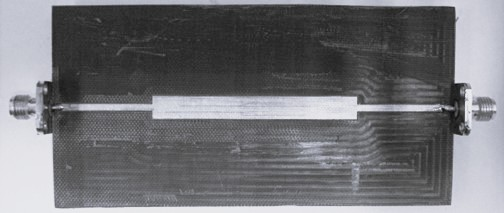
\includegraphics[width=\textwidth]{fig/ch3/microstripe_width_change_real_measurement.jpg}
         
         \caption{}
         \label{fig:microstripe_width_change_real_measurement_wide}
     \end{subfigure}
     \hfill
     \begin{subfigure}{0.44\textwidth}
         \centering
         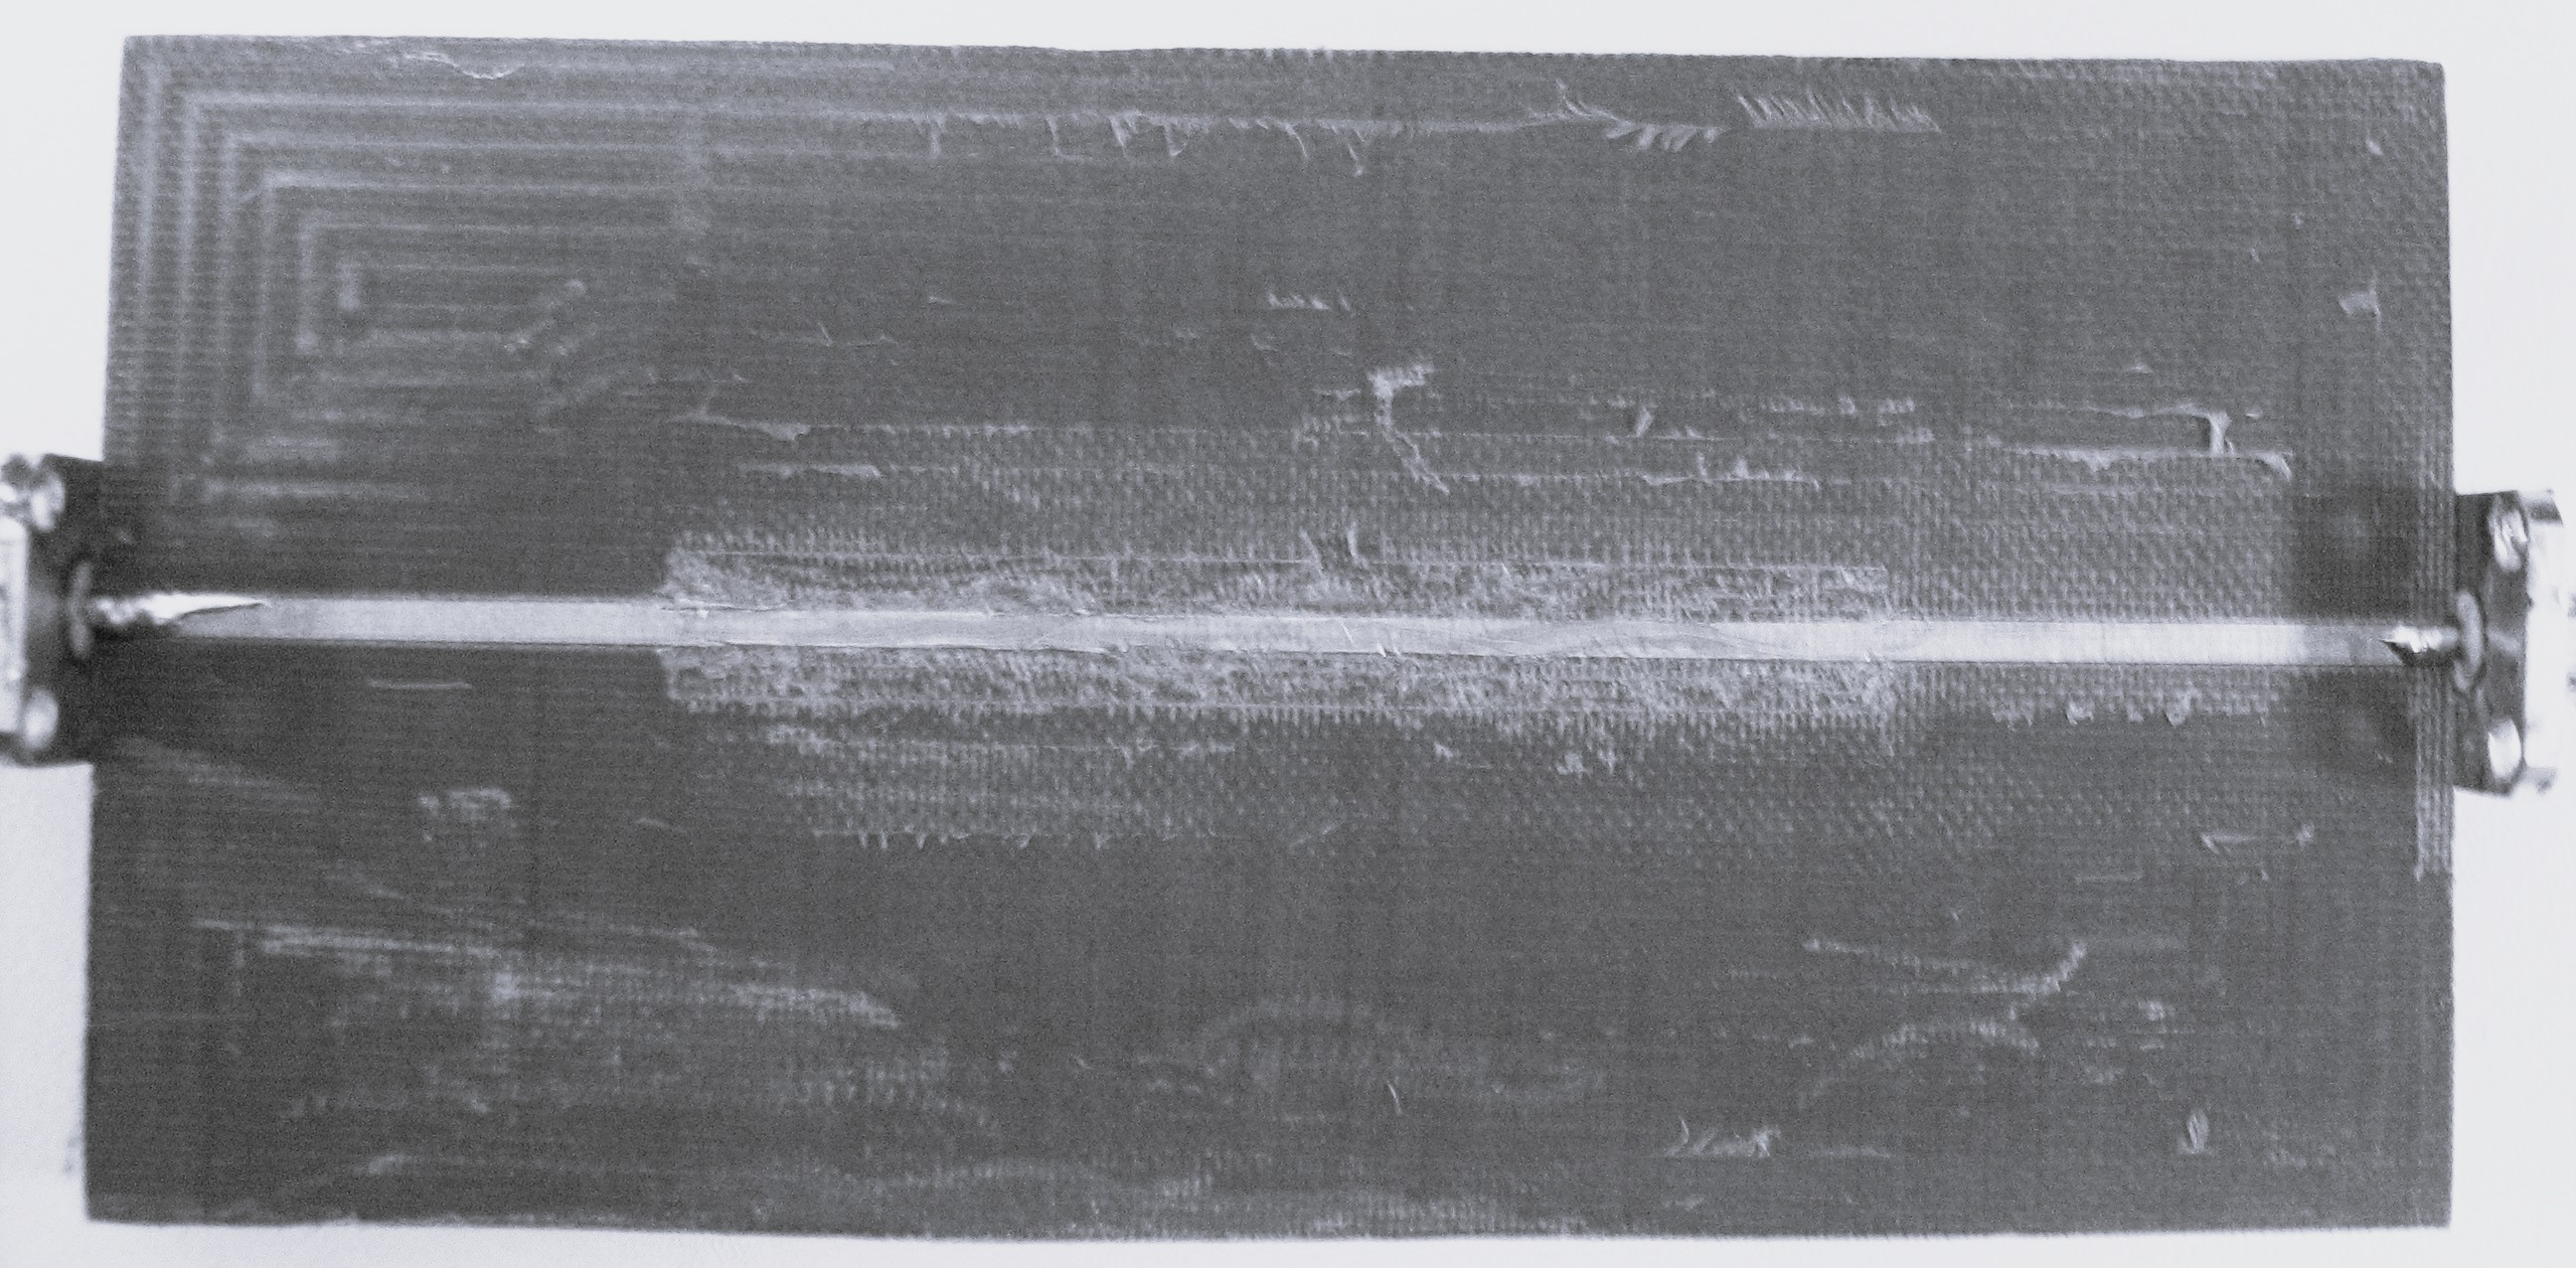
\includegraphics[width=\textwidth]{fig/ch3/microstripe_width_change_real_measurement_thin.jpg}
         
         \caption{}
         \label{fig:microstripe_width_change_real_measurement_thin}
     \end{subfigure}
     \hfill
     \begin{subfigure}{0.35\textwidth}
         \centering
         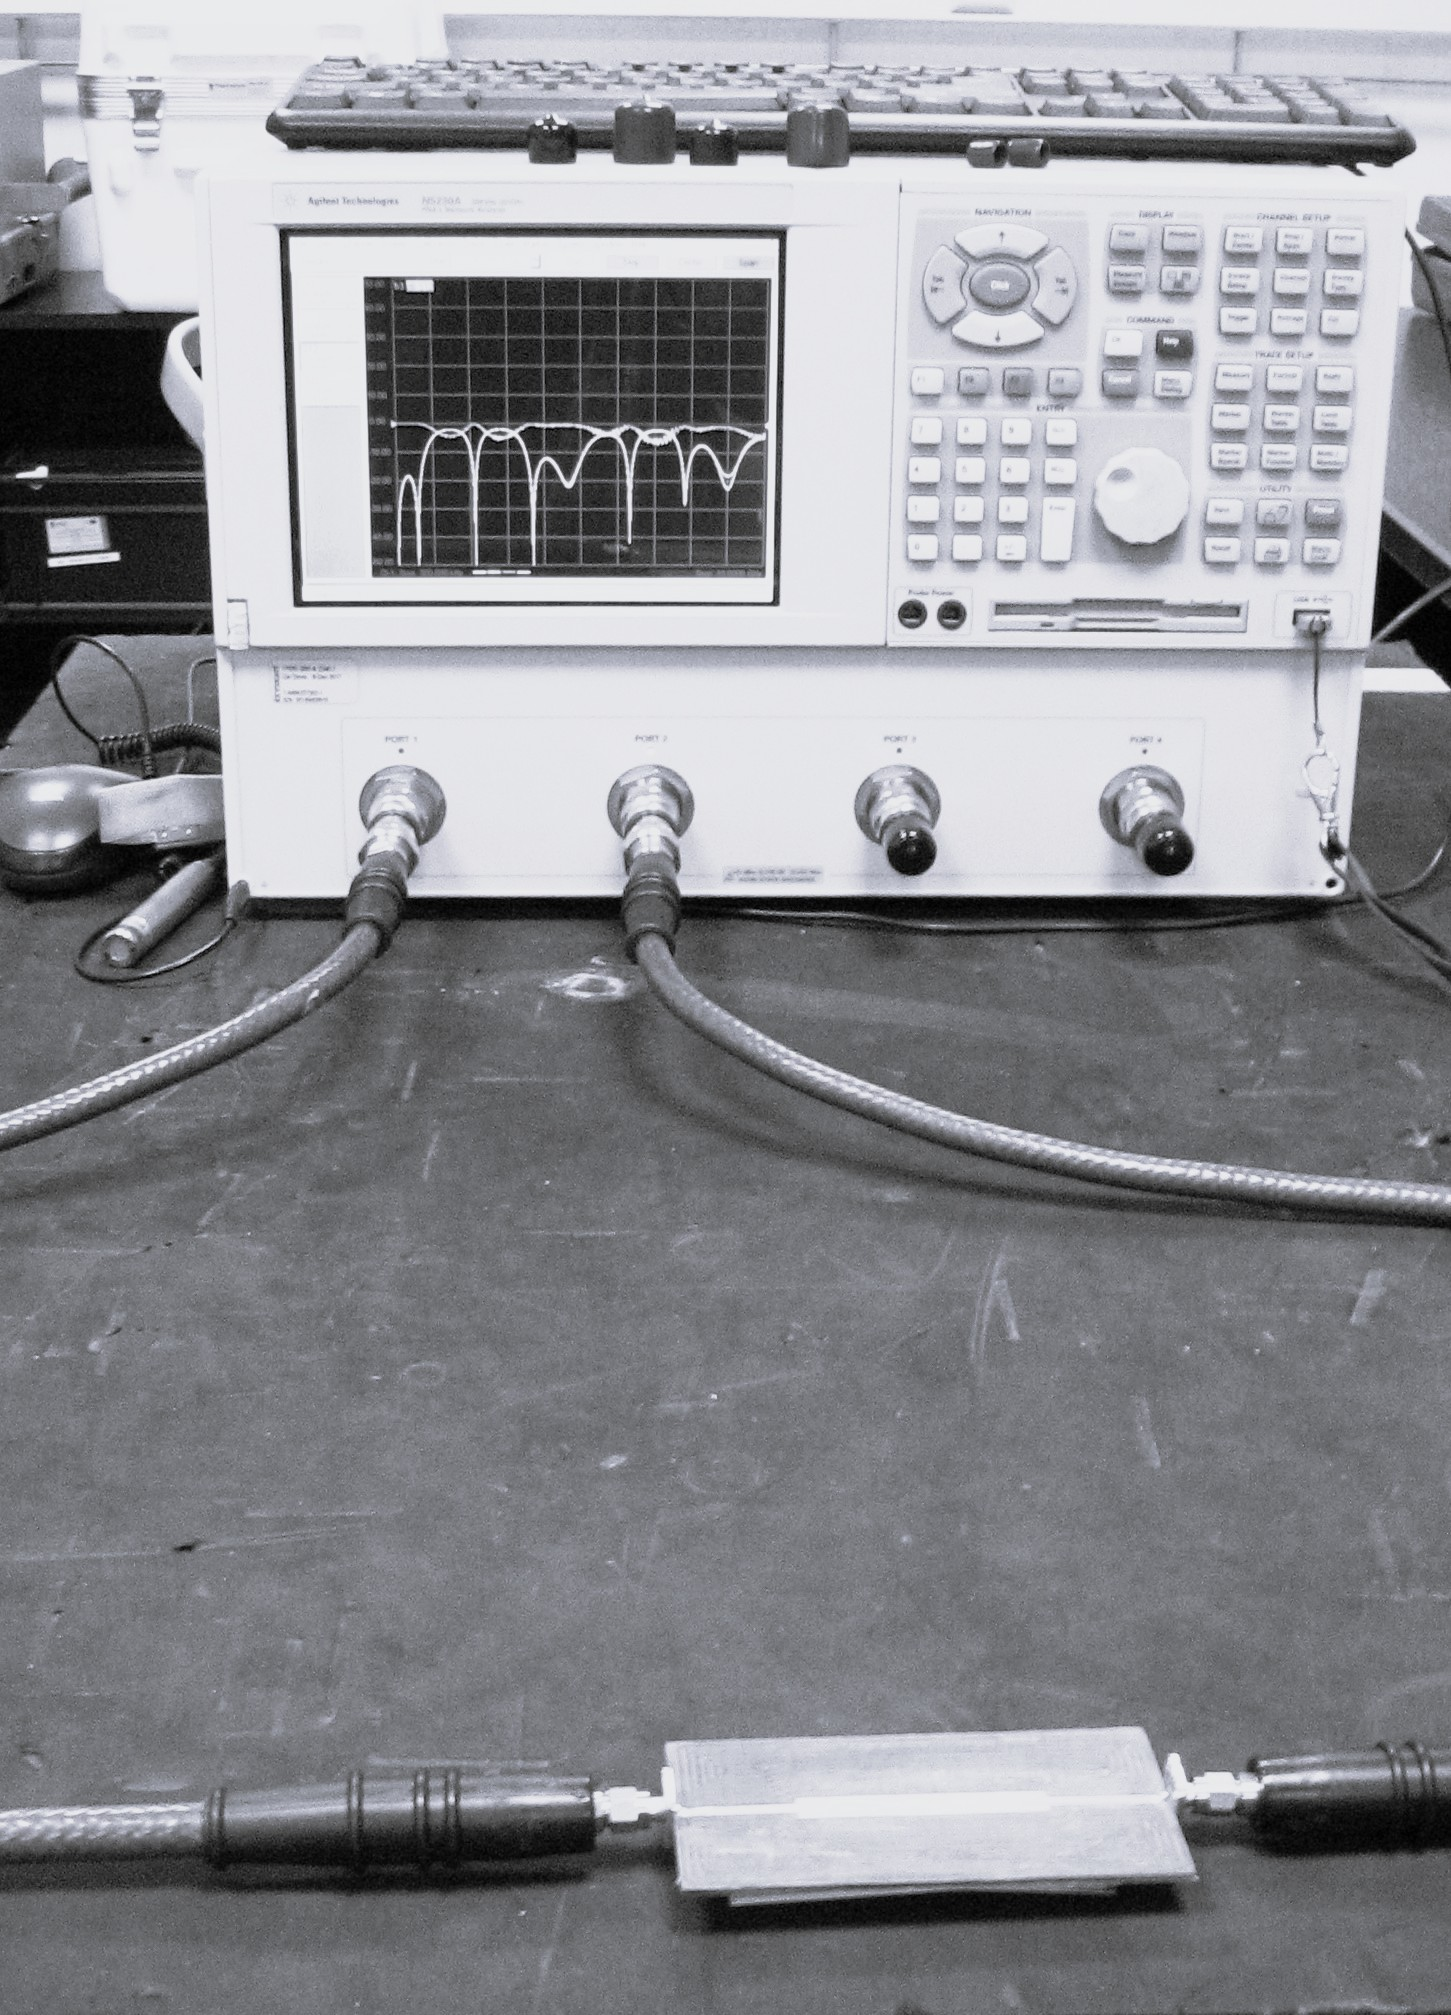
\includegraphics[width=1\textwidth]{fig/ch3/microstrip_width_change_testbench}
         
         \caption{}
         \label{fig:microstripe_width_change_real_measurement_testbench}
     \end{subfigure}
     
     \caption{Transmisyjna linia mikropaskowa zbudowana na laminacie mikrofalowym Rogers Ultralam 2000: a) przed modyfikacją b) po modyfikacji c) stanowisko pomiarowe.} \label{fig:testbench}
\end{figure}

\subsection{Model kaskadowy}

W dalszych rozważaniach przyjęto, że modyfikacja środkowego segmentu linii polega na jego zwężeniu. Model kaskady z symetryczną nieciągłością skokową przedstawiono na rys. \ref{fig:microstripe_width_change_cascade_t1} \cite{cite:doktorat} i składa się on z następujących elementów reprezentowanych przez macierze łańcuchowe: lewostronne złącze SMA ($T_{CL}$), lewostronną węższą linię mikropaskową ($T_{lc}$) o szer. $w_2$ i dł. $l_c$, lewostronną nieciągłość skokową ($T_{SL}$), szeroką linię mikropaskową ($T_{L1}$) o szer. $w_1$ i dł. $l$ tworzącą środkowy segment linii mikropaskowej, prawostronną nieciągłość skokową ($T_{SR}$), prawostronną węższą linię mikropaskową ($T_{lc}$) o szer. $w_2$ i dł. $l_c$ oraz prawostronne złącze SMA ($T_{CR}$). Z kolei model bez nieciągłości skokowej (rys. \ref{fig:microstripe_width_change_cascade_t2} \cite{cite:doktorat}) składa się z lewostronnego złącza SMA ($T_{CL}$), lewostronnej węższej linii mikropaskowej ($T_{lc}$) o szer. $w_2$ i dł. $l_c$, wąskiej linii mikropaskowej ($T_{L1}$) o~szer. $w_2$ i dł. $l$ tworzącą środkowy segment linii mikropaskowej, prawostronnej węższej linii mikropaskowej ($T_{lc}$) o szer. $w_2$ i dł. $l_c$ oraz prawostronnego złącza SMA ($T_{CR}$).

Procedurę ekstrakcji stałej dielektrycznej rozpoczyna się od sytuacji przedstawionej na rys. \ref{fig:microstripe_width_change_cascade_t1} (przed modyfikacją), którą opisuje poniższe równanie \cite{cite:two_lines_method_trace}:

\begin{figure}[tbh!]
     \centering
     \begin{subfigure}[b]{1\textwidth}
         \centering
         %\hspace*{-0.15\textwidth}
         {\includesvg[inkscapelatex=false,width=1\textwidth]{fig/ch3/cascade_t1}
         \caption{}
         \label{fig:microstripe_width_change_cascade_t1}}
     \end{subfigure}
     \hfill
     \begin{subfigure}[b]{1\textwidth}
         \centering
         {\includesvg[inkscapelatex=false,width=1\textwidth]{fig/ch3/cascade_t2}}
         \caption{}
         \label{fig:microstripe_width_change_cascade_t2}
     \end{subfigure}
        \caption{Kaskada dwuwrotników opisanych za pomocą macierzy łańcuchowych dla układu z rys.~\ref{fig:microstripe_width_change_schematic}: a)~przed modyfikacją b) po modyfikacji}
        \label{fig:microstripe_width_change_cascade}
\end{figure}

 \begin{equation}
    \label{cascade_main_eq}
      T=T_L\cdot T_{SL}\cdot T_{L1}\cdot T_{SR}\cdot T_R \text{,}
 \end{equation}

\noindent przy czym:

\begin{equation}
    \label{cascade_main_1_eq}
      T_L = T_{CL} \cdot T_{lc} \text{,}
 \end{equation}

    \begin{equation}
    \label{cascade_main_2_eq}
      T_R = T_{lc} \cdot T_{CR} \text{.}
 \end{equation}

 \noindent Kluczowym uproszczeniem i głównym źródłem błędu przedstawionej metody jest założenie równości obu nieciągłości skokowych, co umożliwia wprowadzenie następujących założeń \cite{cite:two_lines_method_trace}:

    \begin{equation}
    \label{cascade_main_3_eq}
      T_{SL} = T_{SR} =T_{S} \text{.}
 \end{equation}

 \noindent W efekcie otrzymujemy poniższe zależności opisujące linię mikropaskową przed i po modyfikacji środkowego segmentu: 

  \begin{equation}
    \label{cascade_main_extended_eq}
      T_1=T_L\cdot T_{S}\cdot T_{L1}\cdot T_{S}\cdot T_R \text{,}
 \end{equation}

    \begin{equation}
    \label{cascade_main_extended_after_modification_eq}
      T_2=T_{L} \cdot T_{L2} \cdot T_{R} \text{.}
 \end{equation}

\noindent Przeprowadzając operację mnożenia macierzy otrzymuje się poniższe równanie:

   \begin{equation}
    \label{cascade_main_extended_2_eq}
     T_2^{-1}T_1=T_R^{-1}T_{L2}^{-1}T_L^{-1}\cdot T_LT_ST_{L1}T_S T_R = T_R^{-1}T_{L2}^{-1} \cdot T_ST_{L1}T_S T_R \text{,}
 \end{equation}

\noindent a korzystając z właściwości śladu macierzy dostajemy następującą zależność:

   \begin{equation}
    \label{cascade_main_extended_3_eq}
      TR=Tr\left(T_2^{-1}T_1\right)\ =Tr\left(T_{L2}^{-1}T_ST_{L1}T_S\right)=Tr\left(T_{M2}^{-1}T_{M1}\right) \text{,}
 \end{equation}

\noindent przy czym:

   \begin{equation}
    \label{cascade_main_extended_4_eq}
      T_{M1}=T_ST_{L1}T_S,
 \end{equation}

    \begin{equation}
    \label{cascade_main_extended_5_eq}
      T_{M2}=T_{L2} \text{.}
 \end{equation}

 \noindent Każdy z elementów składowych kaskady (\ref{cascade_main_extended_3_eq}) jest zależny od mierzonej stałej dielektrycznej podłoża \cite{cite:doktorat}:

  \begin{align}
   \begin{split}
    \label{cascade_main_epsilon_dependant_eq}
      TR \left( \varepsilon_r \right)&=
      Tr\left(T_2^{-1}\left( \varepsilon_r \right)T_1\left( \varepsilon_r \right)\right)\ = \\
  &=Tr\left(T_{M2}^{-1}\left( \varepsilon_r \right)T_{M1}\left( \varepsilon_r \right)\right)= \\
        &=Tr\left(T_{L2}^{-1}\left( \varepsilon_r \right)T_S\left( \varepsilon_r \right)T_{L1}\left( \varepsilon_r \right)T_S\left( \varepsilon_r \right)\right) \text{.}
 \end{split}    
 \end{align}




\subsection{Macierze łańcuchowe}

Model numeryczny wykorzystany w metodzie ze zmianą szerokości linii mikropaskowej wykorzystuje transmisyjną macierz ABCD linii mikropaskowej przedstawioną poniżej \cite{cite:microstrip_book}:

  \begin{figure}[tbh!]
     \centering
     \begin{subfigure}[b]{0.49\textwidth}
         \centering
         %\hspace*{-0.15\textwidth}
         {\includesvg[inkscapelatex=false,width=0.6\columnwidth]{fig/ch3/step_discontinuity_physical}}
         \caption{}
         \label{fig:step_discontinuity_physical}
     \end{subfigure}
     \hfill
     \begin{subfigure}[b]{0.49\textwidth}
         \centering
         {\includesvg[inkscapelatex=false,width=0.6\columnwidth]{fig/ch3//step_discontinuity_schematic}}
         \caption{}
         \label{fig:step_discontinuity_schematic}
     \end{subfigure}
        \caption{Mikropaskowa nieciągłość skokowa: a) reprezentacja fizyczna
b) model obwodowy.}
        \label{fig:step_discontinuity}
\end{figure}



\begin{equation}
    \label{microstrip_T_matrix_general_eq}
     T= \begin{bmatrix}
          \cos{\left( \gamma_c L \right)} & j \cdot Z_c\sin{\left( \gamma_c L \right)} \\
          j \cdot \cfrac{1}{Z_c} \sin{\left( \gamma_c L \right)} & \cos{\left( \gamma_c L \right)}
      \end{bmatrix} \text{,}
 \end{equation}

 \noindent gdzie $L$ to długość linii mikropaskowej, $Z_c$ to jej impedancja charakterystyczna, a $\gamma_c$ to stała propagacji. Wprowadzono również zastępczy model nieciągłości skokowej (rys. \ref{fig:step_discontinuity} \cite{cite:microstrip_book}) w formie kaskady macierzy transmisyjnych \cite{cite:microstrip_book,cite:pozar}:

 \begin{equation}
    \label{step_discontinuity_matrix_general_eq}
      T_{SD} = T_{L_{s_1}} \cdot T_{C_p} \cdot T_{L_{s_2}} \text{,}
 \end{equation}

 \begin{equation}
    \label{step_discontinuity_matrix_eq}
      T_{SD} = \begin{bmatrix} 1 & j\omega L_{s_1} \\ 0 & 1 \end{bmatrix} \cdot \begin{bmatrix} 1 & 0 \\ j\omega C_p & 1 \end{bmatrix}
      \cdot \begin{bmatrix} 1 & j\omega L_{s_2} \\ 0 & 1 \end{bmatrix} \text{,}
 \end{equation}
\begin{equation}
    \label{step_discontinuity_matrix_2_eq}
      T_{SD} =  \begin{bmatrix}
      1 - \omega^2 L_{s_1}C_{p} &j\omega L_{s1} + j\omega L_{s2} \cdot \left( 1 - \omega^{2} L_{s_1} C_{p} \right) \\ 
      j\omega C_p & 1 - \omega^2 L_{s_2} C_{p} \end{bmatrix} \text{,}
 \end{equation}

\noindent przy czym:

 \begin{equation}
    \label{step_discontinuity_3_eq}
      L_{s_1}=\frac{L_{w1}}{L_{w1}+L_{w2}}L_s \text{,}
 \end{equation}
\begin{equation}
    \label{step_discontinuity_4_eq}
      L_{s_2}=\frac{L_{w2}}{L_{w1}+L_{w2}}L_s \text{,}
 \end{equation}
   \begin{equation}
    \label{step_discontinuity_eq}
      L_{w1}=\frac{Z_{0m1}\sqrt{\varepsilon_{r_{eff_1}}}}{c}\text{,}
 \end{equation}
\begin{equation}
    \label{step_discontinuity_2_eq}
      L_{w2}=\frac{Z_{0m2}\sqrt{\varepsilon_{r_{eff_2}}}}{c} \text{,}
 \end{equation}
\begin{equation}
    \begin{split}
    \label{step_discontinuity_5_eq}
      C_p &  =0,00137\frac{\sqrt{\varepsilon_{r_{eff_1}}}}{Z_{0m1}}\left(1-\frac{w_2}{w_1}\right)  h \cdot \\ & \cdot \left[\frac{\varepsilon_{r_{eff_1}}+0,3}{\varepsilon_{r_{eff_1}}-0,258}\right] \left[\frac{{w_1/h}+0,264}{{w_1}/{h}+0,8}\right] \;\; \text{(pF),}
      \end{split}
 \end{equation}
\begin{equation}
    \label{step_discontinuity_6_eq}
      L_s=0,000987 \cdot h \cdot \left(1-\frac{Z_{0m1}}{Z_{0m2}}\sqrt{\frac{\varepsilon_{r_{eff_1}}}{\varepsilon_{r_{eff_2}}}}\right)^2 \;\; \text{(nH),} 
 \end{equation}

 \noindent gdzie $h$ to grubość podłoża, $c$ to prędkość światła w próżni, $\omega$ to częstotliwość kątowa, $Z_{0mx}$ i $\varepsilon_{reffx}$ to kolejno impedancja charakterystyczna oraz stałą dielektryczna linii o szerokościach $w_1$ i $w_2$.
 \par W opisanej metodzie przyjęto identyczność macierzy $T$ opisujących lewą i prawą nieciągłość skokową, co wymusiło zmianę modelu zastępczego nieciągłości skokowej (\ref{step_discontinuity_matrix_general_eq})-(\ref{step_discontinuity_2_eq}) w następujący sposób \cite{cite:line_width_method}:

 \begin{equation}
    \label{step_discontinuity_7_eq}
      L_{ser} = L_{s_1} = L_{s_2} = \frac{L_{s_1} + L_{s_2}}{2} = L_{s}/2 \text{,}
 \end{equation}

  \begin{equation}
    \label{step_discontinuity_matrix_general-modified_eq}
      T_{S} = T_{L_{ser}} \cdot T_{C_p} \cdot T_{L_{ser}} \text{,}
 \end{equation}

 \begin{equation}
    \label{step_discontinuity_matrix_modified_eq}
      T_{S} = \begin{bmatrix} 1 & j\omega L_{ser} \\ 0 & 1 \end{bmatrix} \cdot \begin{bmatrix} 1 & 0 \\ j\omega C_p & 1 \end{bmatrix}
      \cdot \begin{bmatrix} 1 & j\omega L_{ser} \\ 0 & 1 \end{bmatrix} \text{,}
 \end{equation}
\begin{equation}
    \label{step_discontinuity_matrix_modified_2_eq}
      T_{S} =  \begin{bmatrix}
      1 - \omega^2 L_{ser}C_{p} &j\omega L_{ser} \cdot \left( 2 - \omega^{2} L_{ser} C_{p} \right) \\ 
      j\omega C_p & 1 - \omega^2 L_{ser} C_{p} \end{bmatrix} \text{.}
 \end{equation}

\noindent Po szczegółowy opis prezentowanej metody odsyłam do \cite{cite:line_width_method} i \cite{cite:doktorat}.

\subsection{Algorytm wyznaczania stałej dielektrycznej} \label{sec:numerical}

Metoda oparta na zmianie szerokości linii mikropaskowej polegaę na wykonaniu pomiarów odbiciowo-transmisyjnych parametrów $S$ przed i po modyfikacji środkowego segmentu linii. Otrzymane dane pozwalają na wyznaczenie lewej strony $LHS$  równania (\ref{cascade_main_extended_3_eq}) \cite{cite:line_width_method};

   \begin{equation}
    \label{cascade_main_extended_3_lhs_eq}
      LHS=Tr\left(T_2^{-1}T_1\right) \text{.}
 \end{equation}

\noindent W przypadku prawej strony równania (\ref{cascade_main_extended_3_eq}):
 
   \begin{equation}
    \label{cascade_main_extended_3_rhs_eq}
      RHS=Tr\left(T_{L2}^{-1}T_ST_{L1}T_S\right) \text{,}
 \end{equation}

 \noindent zaproponowana metoda opiera się na omówionych wcześniej macierzach transmisyjnych modelu nieciągłości skokowej i modelu linii transmisyjnej. Prawa strona równania posiada bardzo skomplikowaną postać, co pokazano w następnej sekcji. 
Algorytm numeryczny wyznaczania stałej dielektrycznej został zaproponowany w~\cite{cite:line_width_method} i składa się z sześciu głównych kroków:
\begin{enumerate}
  \item Przybliżenie szukanej wartości stałej dielektrycznej badanej próbki z~wykorzystaniem rozkładu minimów przebiegu wartości $|S_{11}|$.
  \item Wyznaczenie średniej arytmetycznej przybliżonej wartości stałej dielektrycznej w funkcji częstotliwości.
  \item Obliczenie śladu macierzy łańcuchowej dla częstotliwości z pasma pomiarowego (zakłada się bardzo niski lub zerowy tangens kąta strat badanego podłoża).
   \item Wyznaczenie możliwych rozwiązań równania dla poszukiwanej stałej dielektrycznej z wykorzystaniem poniższej funkcji celu:
       \begin{equation}
    \label{line_width_goal_function_eq}
    GF(\varepsilon_r)=\left| Tr\underbrace{\left( T_2^{-1}\left(\varepsilon_r \right) T_1\left(\varepsilon_r \right) \right)}_{pomiar}-Tr\underbrace{\left(T_{M2}^{-1}\left(\varepsilon_r \right)T_{M1}\left(\varepsilon_r \right)\right)}_{model} \right| \text{.}
 \end{equation}
   \item Przyjęte podejście może skutkować uzyskaniem wielu rozwiązań na dyskretnej częstotliwości. W takim przypadku za rozwiązanie przyjmuje się średnią arytmetyczną możliwych rozwiązań na danej częstotliwości. Jeżeli na danej częstotliwości nie znaleziono rozwiązania, to przyjmuje się najbliższą, niezerową wartość.
   \item Uzyskany w poprzednim kroku rozkład wartości stałej dielektrycznej w~funkcji częstotliwości jest następnie wygładzany i aproksymowany wielomianem trzeciego stopnia.
 
\end{enumerate}

Wyczerpujący opis numerycznej procedury wyznaczania stałej dielektrycznej mierzonego podłoża w metodzie zmiany szerokości linii mikropaskowej przedstawiono w \cite{cite:doktorat}.

\subsubsection{Analityczny wzór na ślad macierzy}

Zaproponowany algorytm numeryczny wyznaczania stałej dielektrycznej podłoża daje prawidłowe rezultaty, lecz jest złożony obliczeniowo i składa się z dużej liczby etapów. Może to powodować trudności w jego implementacji w samodzielnej jednostce wektorowego analizatora sieci, co zmniejsza jego szanse na zastąpienie obecnych szerokopasmowych standardów przemysłowych, tj. metoda różnicowej fazy. Pierwszym etapem w zmniejszeniu złożoności zaproponowanej procedury jest wyznaczenie analitycznego wzoru na ślad macierzy - $RHS$  z równania (\ref{cascade_main_extended_3_eq}), co pokazano poniżej:

\begin{equation}
    a_1 = (2A^2-1)(2B^2-1)-2AB[(C-1)(B+1)+(D-1)(A+1)] \text{,}
\end{equation}

\begin{equation}
    \begin{split}
    a_2 & = -\frac{\omega}{Z_{c1}}[AL_{s1}(A+1)(2B^2-1)-\\
    & -B(L_{s2}A^2(B+1)+L_{s1}(D-1)(A+1)^2)] \text{,}
    \end{split}
\end{equation}

\begin{equation}
    \begin{split}
    a_3 & = -\frac{\omega}{Z_{c2}}[L_{s2}B(B+1)(2A^2-1)-\\
    & -A(L_{s1}B^2(A+1)+L_{s2}(C-1)(B+1)^2)] \text{,}
    \end{split}
\end{equation}

\begin{equation}
    a_4 = -\omega Z_{c1}[C_{p1}A(2B^2-1)-B(C_{p2}A^2+C_{p1}(C-1)(B+1))] \text{,}
\end{equation}

\begin{equation}
    a_5 = -\omega Z_{c2}[C_{p2}B(2A^2-1)-A(C_{p1}B^2+C_{p2}(A+1)(D-1))] \text{,}
\end{equation}

\begin{equation}
    a_6 = -\frac{\omega^2}{2Z_{c1}Z_{c2}}[L_{s2}A(B+1)-L_{s1}B(A+1)]^2 \text{,}
\end{equation}

\begin{equation}
    a_7 = \frac{Z_{c1}}{2Z_{c2}}[(AB-(C-1)(B+1))^2] \text{,}
\end{equation}

\begin{equation}
   a_8 = \frac{Z_{c2}}{2Z_{c1}}[AB-(D-1)(A+1)]^2 \text{,}
\end{equation}

\begin{equation}
    a_9 = -\frac{1}{2}\omega^2Z_{c1}Z_{c2}(C_{p1}B-C_{p2}A)^2 \text{,}
\end{equation}



\begin{equation}
    b_1 = a_2 + a_4 \text{,}
\end{equation}

\begin{equation}
    b_2 = a_3 + a_5 \text{,}
\end{equation}

\begin{equation}
    b_3 = a_6 + a_7 + a_8 + a_9 \text{,}
\end{equation}

\begin{equation}
\label{c1}
    c_1 = 2 b_2 cos(\gamma_1L)sin(\gamma_2L) \text{,}
\end{equation}

\begin{equation}
    c_2 = 2 b_1 sin(\gamma_1L)cos(\gamma_2L) \text{,}
\end{equation}

\begin{equation}
    c_3 = 2 a_1 cos(\gamma_1L)cos(\gamma_2L) \text{,}
\end{equation}

\begin{equation}
\label{c4}
    c_4 = 2 b_3 sin(\gamma_1L)sin(\gamma_2L) \text{,}
\end{equation}

\noindent Korzystając z zależności (\ref{c1})-(\ref{c4}) otrzymuje się analityczną postać prawej strony równania (\ref{cascade_main_extended_3_eq}):

\begin{equation}
\label{eq:trace_analitycal}
     RHS=Tr\left(T_{L2}^{-1}T_ST_{L1}T_S\right) = c_1 + c_2 + c_3 + c_4 \text{,}
\end{equation}

\noindent przy czym:

\begin{equation}
    A = 1 - \omega^2L_{s1}C_{p1} \text{,}
\end{equation}

\begin{equation}
    B = 1 - \omega^2L_{s2}C_{p2} \text{,}
\end{equation}

\begin{equation}
    C = 1 - \omega^2L_{s2}C_{p1} \text{,}
\end{equation}

\begin{equation}
    D = 1 - \omega^2L_{s1}C_{p2} \text{.}
\end{equation}



\noindent gdzie $\omega$ to częstotliwość kątowa, $L$ to długość linii mikropaskowej, $Z_{c1}$, $Z_{c2}$, $C_{p1}$ i $C_{p2}$, $L_{s1}$ i $L_{s2}$ oraz $\gamma_1$ i $\gamma_2$ to impedancje charakterystyczne, pojemności bocznikujące nieciągłości skokowej, symetryczne indukcyjności nieciągłości skokowej (patrz rys. \ref{fig:step_discontinuity_schematic}) oraz stałej propagacji kolejno przed i~po modyfikacji środkowego segmentu linii. W tym miejscu należy również podkreślić, że zmiana szerokości środkowego segmentu linii nie musi prowadzić do usunięcia nieciągłości skokowej. Co więcej, wszystkie wymienione parametry linii mikropaskowej zawierają informację o stałej dielektrycznej mierzonego podłoża.
\par Na rys. \ref{fig:trace_analytical} przedstawiono przykładowy wykres przedstawiający porównanie modułów śladów macierzy $RHS$ w funkcji częstotliwości (wymiary linii: $h$~=~0,762~mm, $t$~=~18~$\mu \text{m}$, $w_1$ = 2,9 mm, $w_2$~=~1,3~mm, $l_c$~=~25~mm, $l$~=~~50 mm; parametry dielektryczne podłoża: $\varepsilon_r$ = 5,275, $\tg\delta$~=~0). Otrzymane rezultaty uzyskano z wykorzystaniem procedury numerycznej oraz przedstawionego w poprzedniej sekcji wzoru analitycznego (\ref{eq:trace_analitycal}). Stwierdzono pełną zgodność pomiędzy obiema metodami obliczeniowymi.

\begin{figure}[tbh]
   \centerline{\includesvg[inkscapelatex=false,width=0.6\columnwidth]{fig/ch3/trace_analytical}}
    \caption{Porównanie śladu macierzy $RHS$ obliczonego numerycznie oraz z~użyciem otrzymanego wzoru analitycznego.}
\label{fig:trace_analytical}
\end{figure}

\section{Wnioski}

Metoda oparta na zmianie szerokości linii mikropaskowej ma duży potencjał do zastąpienia obecnego standardu przemysłowego pomiaru stałej dielektrycznej cienkich podłoży dielektrycznych, tj. metody różnicowej fazy. Niewątpliwą przewagą tej metody jest brak konieczności modyfikacji geometrii podłoża, zniwelowanie błędu związanego z montażem złącz pomiarowych oraz możliwość stosowania szerokiej gamy metod nanoszenia metalizacji. Z~drugiej strony numeryczny algorytm obliczania stałej dielektrycznej mierzonego podłoża stosowany w metodzie ze zmianą szerokości linii mikropaskowej jest złożony obliczeniowo. W efekcie może być trudny do zastosowania w~samodzielnych wektorowych analizatorach sieci. Dodatkowo nie uzyskano jednoznacznych ram stosowalności tej metody oraz wpływu uproszczonego modelu nieciągłości skokowej na błąd metody. W~niniejszej pracy wyprowadzono równanie śladu macierzy umożliwiając tym samym dalsze prace nad optymalizacją metody opartej na zmianie szerokości linii mikropaskowej oraz wprowadzenia jej do szerokiego użycia w warunkach przemysłowych i laboratoryjnych.

\begin{thebibliography}{8}

\bibitem{cite:res1}
Liu, C., Liao, C., Peng, Y., Zhang, W., Wu, B., Yang, P.: Microwave sensors and their applications in permittivity measurement. Sensors (Basel, Switzerland), 24(23), 7696 (2024)

\bibitem{cite:res2}
Alahnomi RA, Zakaria Z, Yussof ZM, Althuwayb AA, Alhegazi A, Alsariera H, Rahman NA.: Review of Recent Microwave Planar Resonator-Based Sensors: Techniques of Complex Permittivity Extraction, Applications, Open Challenges and Future Research Directions. Sensors; 21(7):2267 (2021)

\bibitem{cite:nonres1}
Zechmeister, J., Lacik, J.: Complex relative permittivity measurement of selected 3D-printed materials up to 10 GHz. 2019 Conference on Microwave Techniques (COMITE). Presented at the 2019 Conference on Microwave Techniques (COMITE), Pardubice, Czech Republic (April 2019)

\bibitem{cite:nonres2}
Liu, W., Wang, M., Shi, Y.: A transmission-reflection method for complex permittivity measurement using a planar sensor. IEEE Sensors Journal, 18(10), 4059–4065 (2018)

\bibitem{cite:SPDR}
Krupka, J.: Precise measurements of the complex permittivity of dielectric materials at microwave
frequencies. Materials Chemistry and Physics 79, 2-3, 195–198 (4 2003)

\bibitem{cite:two_lines_method}
Das, N. K., Voda, S. M., Pozar, D. M.: Two Methods for the Measurement of Substrate Dielectric
Constant. IEEE Transactions on Microwave Theory and Techniques 35, 7, 636–642 (1987)

\bibitem{cite:line_width_method}
Szostak K., Slobodzian P.: Broadband dielectric measurement of PCB and substrate materials by means of a microstrip line of adjustable width, IEEE Microw. Wirel. Compon. Lett., vol. 28, no. 10, pp. 945–947 (2018)

\bibitem{cite:doktorat}
Szostak K.: Charakteryzacja parametrów elektrycznych substancji stałych i ciekłych przy użyciu planarnych struktur mikrofalowych [Doctoral dissertation, Wrocław University of Science and Technology] (2024)

\bibitem{cite:two_lines_method_trace}
Lee, M. Q., Nam, S.: An accurate broadband measurement of substrate dielectric constant. IEEE
Microwave and Guided Wave Letters 6, 4, 168–170 (4 1996)

\bibitem{cite:microstrip_book}
Garg, R., Bahl, I., Bozzi M.: Microstrip Lines and Slotlines, 3rd ed. Artech House (2013)

\bibitem{cite:pozar}
Pozar M. D.: Microwave Engineering, 4th Edition, 4th ed. Wiley (2011)

\end{thebibliography}
\chapterauthor{Thanh-Ngo Nguyen}
\chapter[Częste eksplorowani \ldots]{Częste eksplorowanie wzorców: kompleksowy przegląd}
\thispagestyle{empty}
\vspace{-8mm} {\large Thanh-Ngo Nguyen} \vspace{8mm}


% =====================
% I. Introduction
% =====================
\section{Introduction}
Eksploracja częstych wzorców (FPM) ma na celu wydobywanie często współwystępujących wzorców z dużych zbiorów danych i stanowi jedno z centralnych zagadnień w odkrywaniu wiedzy oraz eksploracji danych. Od czasu przełomowej pracy Agrawala i Srikanta dotyczącej eksploracji reguł asocjacyjnych w 1993 roku~\cite{agrawal1994fast}, intensywne badania doprowadziły do znacznego rozwoju efektywności, skalowalności i zastosowań FPM w różnych środowiskach obliczeniowych.

Metody FPM znalazły szerokie zastosowanie m.in. w analizie koszyka zakupowego, systemach rekomendacyjnych, modelowaniu zachowań, eksploracji danych internetowych, cyberbezpieczeństwie, bioinformatyce oraz wielu innych obszarach. W tych zastosowaniach częste wzorce dostarczają interpretowalnych struktur, które mogą być bezpośrednio analizowane przez ekspertów dziedzinowych. FPM często stanowi kluczowy element szerszego procesu analitycznego, w którym wydobyte wzorce są dalej wykorzystywane do generowania reguł, klasyfikacji, klasteryzacji, wykrywania anomalii lub wspomagania decyzji.

Niniejszy rozdział przedstawia kompleksowy przegląd FPM, obejmujący podstawowe pojęcia, reprezentatywne algorytmy eksploracji wzorców (eksplorację zbiorów przedmiotów, wzorców sekwencyjnych oraz podgrafów), miary oceny, zastosowania dziedzinowe oraz nowe kierunki badań. Materiał ten jest przeznaczony dla czytelników zainteresowanych zarówno teoretycznymi aspektami, jak i~praktycznym wdrażaniem metod eksploracji częstych wzorców we współczesnych środowiskach zorientowanych na dane.

% =====================
% II. Fundamental Concepts
% =====================
\section{Podstawowe pojęcia}
\label{sec:fundamentals}
Niech $I = \{A,B,C,D\}$ będzie skończonym zbiorem przedmiotów (ang. \textit{items}). Baza danych transakcji $D$ składa się z transakcji $T_k$, gdzie $T_k \subseteq I$. Rozważamy przykładową bazę danych przedstawioną w Tabeli~\ref{tab:dataset}.

\begin{table}[ht]
\centering
\caption{Przykładowa baza danych transakcji}
\label{tab:dataset}
\begin{tabularx}{.5\textwidth}{cC}
\toprule
TID & Przedmioty \\
\midrule
1 & A, B, C, D \\
2 & A, C, D \\
3 & B, C \\
4 & A, B \\
5 & A, B, C \\
\bottomrule
\end{tabularx}
\end{table}

\emph{Zbiorem przedmiotów} (ang. \textit{itemset}) $X$ nazywamy dowolny podzbiór $I$. Jego (względne) wsparcie definiuje się następująco:

\begin{equation}
\label{eq:support}
support(X) = \frac{|\{T_k \in D \mid X \subseteq T_k \}|}{|D|}.
\end{equation}

Przy $|D| = 5$ oraz progu minimalnego wsparcia $minsup = 60\%$ (tj. co najmniej trzy transakcje), obliczamy wsparcie wybranych zbiorów przedmiotów następująco:

\begin{equation}\scriptstyle
support(A) = \frac{4}{5},\; support(B) = \frac{4}{5},\; support(C) = \frac{4}{5},\; support(D) = \frac{3}{5},\nonumber
\end{equation}
\begin{equation}\scriptstyle
support(AB) = \frac{3}{5},\; support(AC) = \frac{3}{5},\; support(AD) = \frac{2}{5},\nonumber
\end{equation}
\begin{equation}\scriptstyle
support(BC) = \frac{3}{5},\; support(BD) = \frac{2}{5},\; support(CD) = \frac{2}{5},\nonumber
\end{equation}
\begin{equation}\scriptstyle
support(ABC) = \frac{2}{5},\; support(ABD) = \frac{1}{5},\; support(ACD) = \frac{2}{5},\; support(BCD) = \frac{1}{5},\nonumber
\end{equation}
\begin{equation}\scriptstyle
support(ABCD) = \frac{1}{5}.
\end{equation}

Zatem częstymi zbiorami przedmiotów są:
\begin{equation}
L_1 = \{A:4, B:4, C:4, D:3\},
\end{equation}
\begin{equation}
L_2 = \{AB:3, AC:3, AD:2, BC:3, BD:2, CD:2\}.
\end{equation}
Zbiór $ABCD$ nie jest częsty, ponieważ jego wsparcie ($\frac{1}{5}$) jest poniżej minimalnego progu wsparcia $60\%$.

Regułę asocjacyjną $X \Rightarrow Y$ (gdzie $X \cap Y = \emptyset$) ocenia się za pomocą ufności (ang. \textit{confidence}):
\begin{equation}
\label{eq:confidence}
confidence(X \Rightarrow Y) = \frac{support(X \cup Y)}{support(X)}.
\end{equation}

Reguła $X \Rightarrow Y$ może być dodatkowo oceniana za pomocą miar interesowności, takich jak \emph{lift}:
\begin{equation}
lift(X \Rightarrow Y) = \frac{support(X \cup Y)}{support(X)\,support(Y)}.
\end{equation}

Miara wsparcia jest \emph{antymonotoniczna}: jeśli $X$ jest nieczęsty, to każdy nadzbiór $X$ również będzie nieczęsty. Właściwość ta jest kluczowa dla odcinania przestrzeni przeszukiwań w klasycznych algorytmach FPM.



% =====================
% III. Taxonomy
% =====================
\section[Taksonomia technik eksploracji \ldots]{Taksonomia technik eksploracji częstych wzorców}
\label{sec:taxonomy}
Techniki eksploracji częstych wzorców można kategoryzować na podstawie strategii przeszukiwania, sposobu reprezentacji danych oraz celów eksploracji. Wysokopoziomowa taksonomia przedstawiona jest w Tabeli~\ref{tab:taxonomy}.

\begin{table}[ht]
    \centering
    \caption{Taksonomia technik eksploracji częstych wzorców}
    \label{tab:taxonomy}
    \begin{tabularx}{.8\textwidth}{LL}
        \toprule
        Kategoria & Reprezentatywne algorytmy \\ 
        \midrule
        Algorytmy Apriori (generowanie kandydatów) & Apriori\\ 
        Wzrost wzorca (projekcja warunkowa) & FP-Growth, PrefixSpan \\ 
        Eksploracja pionowa (TID-zbiory) & Eclat, dEclat, SPADE \\ 
        Eksploracja grafów/drzew & gSpan, GRAMI, OWGraMi \\          
        \bottomrule
    \end{tabularx}
\end{table}

Każda kategoria oferuje odmienne kompromisy pod względem czasu wykonania, użycia pamięci, łatwości implementacji oraz przydatności dla różnych charakterystyk danych.


% =====================
% IV. Representative Algorithms
% =====================
\section{Reprezentatywne algorytmy}
\label{sec:algorithms}
Niniejsza sekcja przedstawia reprezentatywne algorytmy, które w znaczący sposób wpłynęły na rozwój eksploracji częstych wzorców. Dyskusja koncentruje się na algorytmach Apriori, FP-Growth oraz Eclat. Dodatkowo omawiamy algorytmy PrefixSpan, SPAM i SPADE dla eksploracji wzorców sekwencyjnych oraz gSpan, GRAMI i OWGraMi dla eksploracji podgrafów.


% --- Apriori ---
\subsection{Algorytm Apriori}
Algorytm Apriori~\cite{agrawal1994fast} wykonuje przeszukiwanie wszerz (ang. \textit{breadth-first search}) po kracie zbiorów przedmiotów. Wykorzystuje on własność domknięcia w dół: wszystkie niepuste podzbiory częstego zbioru przedmiotów również muszą być częste. W związku z tym każdy kandydat posiadający nieczęsty podzbiór może zostać odrzucony (przycięty).



\begin{algorithm}[!htb]
\LinesNumbered
\SetKwInOut{Input}{Input}\SetKwInOut{Output}{Output}

\Input{$D$: Transaction database, $I$: Set of items, $minsup$: Minimum support threshold}
\Output{$F$: Set of all frequent itemsets}
\BlankLine

$F \leftarrow \emptyset$ \\
$k \leftarrow 1$ \\
$C_1 \leftarrow \{\{i\} \mid i \in I\}$ \tcp*[r]{Initial candidate 1-itemsets}

\While{$C_k \neq \emptyset$}{
    \textnormal{ComputeSupport}$(C_k, D)$ \\
    
    \ForEach{itemset $X \in C_k$}{
        \If{$support(X) \ge minsup$}{
            $F \leftarrow F \cup \{X\}$ \\
        }
    }
    
    Remove all infrequent itemsets from $C_k$ \\
    
    $C_{k+1} \leftarrow$ \textnormal{GenerateCandidates}$(F)$ \tcp*[r]{Join + prune step}
    
    $k \leftarrow k + 1$ \\
}

\Return $F$
\caption{Algorytm Apriori}
\label{alg:apriori}
\end{algorithm}

\begin{algorithm}[!htb]
\LinesNumbered
\SetKwInOut{Input}{Input}\SetKwInOut{Output}{Output}


\BlankLine

\ForEach{transaction $t \in D$}{
    \ForEach{$k$-subset $X \subseteq t$}{
        \If{$X \in C_k$}{
            $support(X) \leftarrow support(X) + 1$
        }
    }
}
% \caption{ComputeSupport($C_k$, $D$)}
% \label{alg:compute_support}
\caption{\textbf{Procedure} ComputeSupport$(C_k, D)$ — wywoływane przez algorytm Apriori}
\label{proc:compute_support}
\end{algorithm}


\begin{algorithm}[!htb]
\LinesNumbered
\SetKwInOut{Input}{Input}\SetKwInOut{Output}{Output}

\Input{$C_k$: Current prefix-tree of frequent $k$-itemsets}
\Output{$C_{k+1}$: Extended prefix-tree (candidate $(k+1)$-itemsets)}
\BlankLine

\ForEach{leaf $X_a \in C_k$}{
    \ForEach{leaf $X_b \in siblings(X_a)$ such that $b > a$}{
        $X_{ab} \leftarrow X_a \cup X_b$ \\
        \tcp{Prune if any $(k)$-subset of $X_{ab}$ is infrequent}
        \If{$\forall X_j \subset X_{ab}$ and $|X_j| = |X_{ab}| - 1$, $X_j \in C_k$}{
            Add $X_{ab}$ as a child of $X_a$ with $support(X_{ab}) \leftarrow 0$
        }
    }
    \If{no extensions from $X_a$}{
        Remove $X_a$ and all its ancestors with no further extensions
    }
}

\Return $C_{k+1}$
\caption{\textbf{Procedure} ExtendPrefixTree$(C_k)$ — wywoływane przez algorytym Apriori}
\label{proc:extend_prefix}
\end{algorithm}

Dla przykładowej bazy danych oraz $minsup = 3$ algorytm Apriori wyznacza:
\begin{equation}
L_1 = \{A:4, B:4, C:4\},\quad
\end{equation}
\begin{equation}
L_2 = \{AB:3, AC:3, BC:3\},\quad
\end{equation}
\begin{equation}
L_3 = \emptyset,
\end{equation}
ponieważ $support(ABC) = 2 < 3$.

Apriori jest algorytmem prostym i intuicyjnym, lecz może generować dużą liczbę kandydatów oraz wymaga wielokrotnego pełnego skanowania bazy danych, co czyni go mniej odpowiednim dla zbiorów gęstych lub bardzo dużych. Pełna procedura algorytmu Apriori została zilustrowana w Algorytmach 1–3.


% --- FP-Growth ---
\subsection{Algorytm FP-Growth}
FP-Growth~\cite{han2000mining} eliminuje generowanie kandydatów poprzez kompresję bazy danych do struktury FP-Tree, a następnie wykonywanie rekurencyjnego wzrostu wzorca na drzewach warunkowych.

Podczas konstruowania FP-Tree transakcje są porządkowane zgodnie z malejącym wsparciem globalnym przedmiotów. W naszym przykładzie $support(A) = support(B) = support(C) = 4$, a do rozstrzygania remisów przyjmujemy porządek:
\begin{equation}
A > B > C > D
\end{equation}
Każda transakcja jest odpowiednio sortowana, a przedmioty nieczęste (w tym przypadku żadne) są usuwane.

Ogólny schemat działania algorytmu FP-Growth wygląda następująco:


\begin{algorithm}[!htb]
\LinesNumbered
\SetKwInOut{Input}{Input}\SetKwInOut{Output}{Output}
\Input{$R$: FP-tree of database $D$; $P$: current prefix (initially $\emptyset$); $minsup$}
\Output{$F$: set of frequent itemsets}
\BlankLine
Remove all infrequent items from $R$ \;
\If{\textnormal{$R$ is a single path}}{
    \ForEach{subset $Y \subseteq R$}{
        $X \leftarrow P \cup Y$ \;
        $support(X) \leftarrow \min\{ count(x) \mid x \in Y \}$ \;
        Add $(X, support(X))$ to $F$ \;
    }
}
\Else{
    \ForEach{frequent item $i$ in $R$ (in increasing support order)}{
        $X \leftarrow P \cup \{i\}$ \;
        $support(X) \leftarrow support(i)$ \tcp{sum of counts of nodes labeled $i$} \;
        Add $(X, support(X))$ to $F$ \;
        $R_X \leftarrow \emptyset$ \tcp{projected FP-tree for $X$} \;
        \ForEach{path in $R$ ending in item $i$}{
            $c \leftarrow$ count of $i$ in that path \;
            Insert prefix of path (excluding $i$) into $R_X$ with count $c$ \;
        }
        \If{$R_X \neq \emptyset$}{
            \textnormal{FPGrowth}$(R_X, X, F, minsup)$ \;
        }
    }
}
\caption{\textbf{FP-Growth} Algorytm}
\label{alg:fpgrowth}
\end{algorithm}


FP-Growth jest zazwyczaj szybszy od algorytmu Apriori w przypadku gęstych zbiorów danych, ponieważ unika generowania i testowania ogromnej liczby kandydatów. Szczegóły algorytmu FP-Growth przedstawiono w Algorytmie 4.


% --- Eclat ---
\subsection{Algorytm Eclat}
Eclat~\cite{zaki2000scalable} (Equivalence Class Transformation) jest algorytmem eksploracji pionowej. Zamiast przechowywać transakcje w postaci list przedmiotów, dla każdego przedmiotu przechowuje on zbiór identyfikatorów transakcji (TID-zbiór), w których dany przedmiot występuje. Dla przykładowej bazy danych:


\begin{table}[ht]
\centering
\caption{Pionowa reprezentacja TID-zbiorów dla przykładu}
\label{tab:eclat_vertical}
\begin{tabularx}{.5\textwidth}{cC}
\toprule
Item & TID-set \\
\midrule
A & \{1, 2, 4, 5\} \\
B & \{1, 3, 4, 5\} \\
C & \{1, 2, 3, 5\} \\
D & \{1, 2\} \\
\bottomrule
\end{tabularx}
\end{table}

Wsparcie zbioru przedmiotów jest równe liczności przecięcia odpowiednich TID-zbiorów, np.:
\begin{equation}
T_{AB} = \{1,4,5\},\quad
T_{AC} = \{1,2,5\},\quad
T_{BC} = \{1,3,5\}.
\end{equation}


\begin{algorithm}[!htb]
\LinesNumbered
\SetKwInOut{Input}{Input}\SetKwInOut{Output}{Output}

\Input{$P$: initial set of frequent 1-itemsets in vertical format $(X, T_X)$; $minsup$}
\Output{$F$: set of frequent itemsets}
\BlankLine

\ForEach{$(X_a, T_{X_a}) \in P$}{
    Add $(X_a, |T_{X_a}|)$ to $F$ \tcp{store frequent itemset}
    
    $P_a \leftarrow \emptyset$ \;
    
    \ForEach{$(X_b, T_{X_b}) \in P$ with $X_b > X_a$}{
        $X_{ab} \leftarrow X_a \cup X_b$ \;
        $T_{X_{ab}} \leftarrow T_{X_a} \cap T_{X_b}$ \;
        
        \If{$|T_{X_{ab}}| \ge minsup$}{
            $P_a \leftarrow P_a \cup \{(X_{ab}, T_{X_{ab}})\}$ \;
        }
    }
    
    \If{$P_a \neq \emptyset$}{
        \textnormal{Eclat}$(P_a, minsup, F)$ \;
    }
}

\caption{\textbf{Eclat} algorytm}
\label{alg:eclat}
\end{algorithm}


\begin{algorithm}[!htb]
\LinesNumbered
\SetKwInOut{Input}{Input}\SetKwInOut{Output}{Output}

\Input{$P$: initial set of frequent 1-itemsets in diffset form $(X, d(X), sup(X))$; $minsup$}
\Output{$F$: set of frequent itemsets}
\BlankLine

\ForEach{$(X_a, d(X_a), sup(X_a)) \in P$}{
    Add $(X_a, sup(X_a))$ to $F$ \tcp{frequent itemset found}
    
    $P_a \leftarrow \emptyset$ \;
    
    \ForEach{$(X_b, d(X_b), sup(X_b)) \in P$ with $X_b > X_a$}{
        $X_{ab} \leftarrow X_a \cup X_b$ \;
        $d(X_{ab}) \leftarrow d(X_b) \setminus d(X_a)$ \;
        $sup(X_{ab}) \leftarrow sup(X_a) - |d(X_{ab})|$ \tcp{diffset support update}
        
        \If{$sup(X_{ab}) \ge minsup$}{
            $P_a \leftarrow P_a \cup \{(X_{ab}, d(X_{ab}), sup(X_{ab}))\}$ \;
        }
    }
    
    \If{$P_a \neq \emptyset$}{
        \textnormal{dEclat}$(P_a, minsup, F)$ \;
    }
}

\caption{\textbf{dEclat} algorytm (diffset-based Eclat)}
\label{alg:declat}
\end{algorithm}




Eclat zmniejsza liczbę skanów bazy danych, lecz może wymagać znacznej ilości pamięci do przechowywania TID-zbiorów w przypadku bardzo dużych zbiorów danych. Algorytm Eclat został przedstawiony w Algorytmie~5.


% --- dEclat ---
\subsection{Algorytm dEclat}
Wydajność algorytmu dEclat~\cite{zaki2003dECLAT} może zostać znacząco poprawiona poprzez redukcję rozmiaru pośrednich TID-zbiorów. Osiąga się to poprzez stosowanie \emph{diffsetów}, które przechowują jedynie różnice między TID-zbiorami, a nie pełne zbiory.

Niech $X_a = \{x_1, \ldots, x_{k-1}, x_a\}$ oraz
$X_b = \{x_1, \ldots, x_{k-1}, x_b\}$, tak że:
\begin{equation}
X_{ab} = X_a \cup X_b = \{x_1, \ldots, x_{k-1}, x_a, x_b\}.
\end{equation}

Diffset zbioru $X_{ab}$ definiuje się jako zbiór transakcji, które zawierają prefiks $X_a$, lecz nie zawierają przedmiotu $x_b$:
\begin{equation}
d(X_{ab}) = t(X_a) \setminus t(X_{ab}) = t(X_a) \setminus t(X_b),
\end{equation}
gdzie $t(X)$ oznacza TID-zbiór dla zbioru przedmiotów $X$.

Możemy dalej wyrazić $d(X_{ab})$ przy użyciu $d(X_a)$ oraz $d(X_b)$ w następujący sposób:
\begin{equation}
d(X_{ab}) = d(X_b) \setminus d(X_a).
\end{equation}


Implikuje to, że operacje przecinania zbiorów w algorytmie Eclat mogą zostać zastąpione bardziej wydajnymi operacjami na diffsetach, co znacząco zmniejsza zużycie pamięci oraz poprawia czas działania. Algorytm dEclat został przedstawiony w Algorytmie~6.



% =====================
% Sequential Pattern Mining
% =====================
\section{Eksploracja wzorców sekwencyjnych}
\label{sec:sequential}
Eksploracja wzorców sekwencyjnych (SPM, ang. \textit{Sequential Pattern Mining})~\cite{agarwal1995spam} stanowi rozszerzenie eksploracji częstych wzorców, ukierunkowane na odkrywanie często występujących sekwencji przedmiotów, zdarzeń lub działań w czasie. Jest szczególnie istotna w takich zastosowaniach jak eksploracja zachowań użytkowników stron WWW, analiza zachowań klientów czy predykcja sekwencji zdarzeń. Dwa reprezentatywne algorytmy SPM to PrefixSpan oraz SPADE.



% ---------------- PrefixSpan ----------------
\subsection{Algorytm PrefixSpan}
PrefixSpan~\cite{pei2001prefixspan} (Prefix-projected Sequential Pattern Mining) jest podejściem typu wzrost wzorca, przeznaczonym do odkrywania częstych wzorców sekwencyjnych bez konieczności generowania dużej liczby sekwencji kandydatów. Zamiast wielokrotnego przeszukiwania całej bazy sekwencji, koncentruje się jedynie na istotnych podsekwencjach poprzez wykorzystanie \emph{baz danych rzutowanych prefiksem}.

Główna idea jest następująca: baza danych jest najpierw skanowana w~celu znalezienia wszystkich częstych elementów jako sekwencji długości 1. Dla każdego częstego prefiksu konstruowana jest baza danych rzutowana, która zawiera wyłącznie sufiksy sekwencji następujące po tym prefiksie. Prefiks jest następnie rekurencyjnie rozszerzany poprzez dołączanie częstych elementów odkrytych w~jego bazie danych rzutowanej. Proces ten jest kontynuowany do momentu, gdy nie można już znaleźć kolejnych częstych rozszerzeń.

Poprzez ograniczenie przestrzeni przeszukiwania do baz danych rzutowanych prefiksem i unikanie jawnego generowania kandydatów, PrefixSpan osiąga wysoką wydajność, szczególnie w przypadku dużych i gęstych zbiorów sekwencyjnych. Algorytm PrefixSpan został przedstawiony w Algorytmie~7.


\begin{algorithm}[!htb]
\LinesNumbered
\SetKwInOut{Input}{Input}\SetKwInOut{Output}{Output}

\Input{$D_r$: projected sequence database for prefix $r$ (or original database if $r = \emptyset$); $minsup$}
\Output{$F$: set of frequent sequential patterns}
\BlankLine

\ForEach{symbol $s \in \Sigma$ such that $sup(s, D_r) \ge minsup$}{
    $r_s \leftarrow r \cdot s$ \tcp{extend prefix by symbol $s$}
    
    Add $(r_s, sup(s, D_r))$ to $F$ \;
    
    $D_s \leftarrow \emptyset$ \tcp{create projected database of $r_s$}
    
    \ForEach{sequence $s_i \in D_r$}{
        $s'_i \leftarrow$ projection of $s_i$ w.r.t.\ symbol $s$ \;
        Remove infrequent symbols from $s'_i$ \;
        \If{$s'_i \neq \emptyset$}{
            Add $s'_i$ to $D_s$ \;
        }
    }
    
    \If{$D_s \neq \emptyset$}{
        \textnormal{PrefixSpan}$(D_s, r_s, minsup, F)$ \;
    }
}

\caption{\textbf{PrefixSpan} algorithm (Prefix-projected Sequential Pattern Mining)}
\label{alg:prefixspan}
\end{algorithm}


% ---------------- SPADE ----------------
\subsection{Algorytm SPADE}
SPADE~\cite{zaki2001spade} (Sequential PAttern Discovery using Equivalence classes) jest algorytmem opartym na pionowym formacie danych, który wydajnie odkrywa wzorce sekwencyjne poprzez wykorzystanie klas równoważności do grupowania podobnych sekwencji. Unika on generowania kandydatów, koncentrując się na rzutowaniu bazy sekwencji na mniejsze podbazy danych. Algorytm SPADE został przedstawiony w Algorytmie~8.


\begin{algorithm}[!htb]
\LinesNumbered
\SetKwInOut{Input}{Input}\SetKwInOut{Output}{Output}

\Input{$P$: set of frequent 1-sequences with ID-lists $L(s)$; $k$: current sequence length; $minsup$}
\Output{$F$: set of frequent sequential patterns}
\BlankLine

\ForEach{$(r_a, L(r_a)) \in P$}{
    Add $(r_a, sup(r_a))$ to $F$ \; \tcp{support = $|L(r_a)|$}
    
    $P_a \leftarrow \emptyset$ \;
    
    \ForEach{$(r_b, L(r_b)) \in P$}{
        $r_{ab} \leftarrow r_a + r_b[k]$ \tcp{join based on same prefix of length $k$}
        $L(r_{ab}) \leftarrow L(r_a) \cap L(r_b)$ \tcp{ID-list intersection}
        
        \If{$sup(r_{ab}) \ge minsup$}{
            $P_a \leftarrow P_a \cup \{(r_{ab}, L(r_{ab}))\}$ \;
        }
    }
    
    \If{$P_a \neq \emptyset$}{
        \textnormal{Spade}$(P_a, minsup, F, k+1)$ \;
    }
}

\caption{\textbf{SPADE} algorithm (Sequential PAttern Discovery using Equivalence classes)}
\label{alg:spade}
\end{algorithm}


% =====================
% Subgraph Mining
% =====================
\section{Eksploracja podgrafów}
\label{sec:subgraph}
Eksploracja podgrafów polega na odkrywaniu częstych podgrafów (lub motywów) w zbiorze danych opartym na grafach, gdzie celem jest znalezienie wzorców, które często występują jako podgrafy w bazie grafów. Jest to szczególnie istotne w takich zastosowaniach jak chemoinformatyka (np. odkrywanie struktur molekularnych), analiza sieci społecznościowych (np. wykrywanie społeczności) oraz sieci biologiczne (np. interakcje białek).

Algorytm gSpan (graph-based Subgraph Pattern Mining)~\cite{yan2002gspan} jest jednym z~najbardziej znanych algorytmów eksploracji częstych podgrafów. gSpan został zaprojektowany w celu wydajnego znajdowania częstych podgrafów w bazach grafowych, wykorzystując strategię przeszukiwania w głąb oraz leksykograficzne porządkowanie reprezentacji grafów.


% ---------------- gSpan ----------------
\subsection{Algorytm gSpan}
Algorytm gSpan~\cite{yan2002gspan} działa poprzez reprezentowanie każdego grafu za pomocą uporządkowanej listy krawędzi oraz wykorzystuje przeszukiwanie w~głąb (ang. \textit{depth-first search}) do eksploracji struktury grafu przy jednoczesnym utrzymaniu porządku leksykograficznego. Zapewnia to, że izomorficzne podgrafy nie są wydobywane wielokrotnie.

gSpan realizuje następujące główne kroki:
\begin{itemize}
    \item Konwersja bazy grafów na uporządkowane listy krawędzi.
    \item Wykonywanie przeszukiwania w głąb w celu generowania kandydatów na podgrafy.
    \item Odrzucanie podgrafów, które nie spełniają minimalnego progu wsparcia.
\end{itemize}

Algorytm gSpan został przedstawiony w Algorytmie~9.



\begin{algorithm}[!htb]
\LinesNumbered
\SetKwInOut{Input}{Input}\SetKwInOut{Output}{Output}

\Input{$C$: current DFS code (initially $\emptyset$);
$D$: graph database; $minsup$}
\Output{$F$: set of frequent subgraph patterns (implicitly stored)}
\BlankLine

$E \leftarrow$ \textnormal{RightMostPath-Extensions}$(C, D)$ \;
\tcp{$E$ contains candidate edge extensions with support}

\ForEach{$(t, sup(t)) \in E$}{
    $C' \leftarrow C \cup t$ \tcp{extend DFS code with edge tuple $t$}
    $sup(C') \leftarrow sup(t)$ \;
    
    \If{$sup(C') \ge minsup$ \textbf{and} \textnormal{IsCanonical}$(C')$}{
        \textnormal{gSpan}$(C', D, minsup)$ \;
    }
}

\caption{\textbf{gSpan} algorithm (graph-based Substructure Pattern Mining)}
\label{alg:gspan}
\end{algorithm}




% ---------------- GRAMI ----------------
\subsection{Algorytm GRAMI}
GRAMI~\cite{elseidy2014grami} (Graph Mining Algorithm for Mining Subgraphs) jest kolejnym algorytmem zaprojektowanym do eksploracji częstych podgrafów, wyposażonym w optymalizacje umożliwiające obsługę wielkoskalowych baz grafów. Wykorzystuje on wydajne strategie przeszukiwania oraz zaawansowane techniki przycinania przestrzeni przeszukiwań. Algorytm GRAMI został przedstawiony w Algorytmie~10.


\begin{algorithm}[!htb]
\LinesNumbered
\SetKwInOut{Input}{Input}\SetKwInOut{Output}{Output}

\Input{$G$: single input graph; $minsup$}
\Output{$F$: set of frequent subgraph patterns}
\BlankLine

Generate frequent 1-edge subgraphs from $G$ and insert them into $F$ \;
Initialize priority queue $PQ$ with frequent 1-edge subgraphs \;

\While{$PQ$ is not empty}{
    $P \leftarrow PQ.\textnormal{pop()}$ \tcp{highest priority pattern}
    
    \ForEach{valid extension $P'$ of $P$}{
        Compute \textnormal{sup}$(P')$ using candidate pairs pruning \;
        
        \If{$sup(P') \ge minsup$}{
            Add $P'$ to $F$ \;
            Insert $P'$ into $PQ$ \;
        }
    }
}

\caption{\textbf{GRAMI} algorithm (Graph Mining via Efficient Candidate Generation)}
\label{alg:grami}
\end{algorithm}


% ---------------- OWGraMi ----------------
\subsection{Algorytm OWGraMi}
Problem eksploracji ważonych podgrafów z ważonego pojedynczego grafu zyskuje coraz większe znaczenie, ponieważ grafy ważone są powszechnie wykorzystywane do reprezentowania, symulowania i monitorowania złożonych i wielkoskalowych systemów, w których każdy obiekt ma różną rolę lub poziom istotności. Tematyka ta przyciąga dużą uwagę badawczą, a wśród istniejących prac podejście Weighted Graph Mining (WeGraMi) jest uważane za reprezentatywny stan wiedzy. Jednakże WeGraMi nie stosuje wczesnej strategii przycinania dla nieważonych podgrafów-kandydatów oraz generuje duże koszty obliczeniowe z powodu konieczności obliczania wag dla wszystkich wydobytych częstych podgrafów.

Aby przezwyciężyć te ograniczenia, Le wraz ze współautorami zaproponował ulepszoną metodę o nazwie Optimized Weighted Graph Mining (OWGraMi)~\cite{le2022owgrami}, która rozszerza WeGraMi, wykorzystując dwie skuteczne strategie optymalizacyjne. Po pierwsze, przycina częste krawędzie, które nie mogą spełnić progu wagowego, zmniejszając liczbę nieważonych kandydatów. Po drugie, ponownie wykorzystuje wagi podgrafów rodzica podczas obliczania wag ich podgrafów potomnych, co znacząco zmniejsza całkowity czas działania. Pełna procedura algorytmu OWGraMi została przedstawiona w Algorytmach 11–12.


% \begin{algorithm}[!htb]
% \LinesNumbered
% \SetKwInOut{Input}{input}\SetKwInOut{Output}{output}

% \Input{$G$: weighted input graph, $minsup$: minimum support, $minWeight$: minimum weight threshold}
% \Output{$F$: set of frequent weighted subgraphs}

% \BlankLine
% $F \leftarrow \emptyset$ \\
% Generate initial frequent edges $C_1$ from $G$ \\
% Prune edges with $weight < minWeight$ \\

% \ForEach{$g \in C_1$}{
%     store $weight(g)$ \\
%     add $g$ into $F$ \\
%     \Call{OWGraMi-Recursive}{$g$, $weight(g)$}
% }
% \Return{$F$}

% \caption{OWGraMi main procedure}
% \label{alg:owgrami}
% \end{algorithm}

\begin{algorithm}[!ht]
\LinesNumbered
\SetKwInOut{Input}{input}\SetKwInOut{Output}{output}
\Input{$G$: weighted input graph, $minsup$: minimum support, $minWeight$: minimum weight threshold}
\Output{$F$: set of frequent weighted subgraphs}
$F \leftarrow \emptyset$ \;
Generate initial frequent edges $C_1$ from $G$ \;
Prune edges with $weight < minWeight$ \;
\ForEach{$g \in C_1$}{
    store $weight(g)$ \;
    add $g$ into $F$ \;
    OWGraMi\_Recursive($g$, $weight(g)$) \;
}
\KwRet{$F$}
\caption{OWGraMi main procedure}
\label{alg:owgrami}
\end{algorithm}



% \begin{algorithm}[!htb]
% \LinesNumbered
% \SetKwInOut{Input}{input}\SetKwInOut{Output}{output}

% \SetKwProg{Fn}{Procedure}{}{}
% \Fn{OWGraMi-Recursive($P$, $w_P$)}{

%     Generate candidate extensions $C_P$ of $P$ \\

%     \ForEach{$X \in C_P$}{
%         Compute edge support of $X$ \\
%         \If{$support(X) \ge minsup$}{
%             Compute $weight(X)$ using:
%             \begin{itemize}
%                 \item reuse $w_P$ as upper bound
%                 \item subtract weighted edges pruned earlier
%             \end{itemize}
%             \If{$weight(X) \ge minWeight$}{
%                 add $X$ to $F$ \\
%                 \Call{OWGraMi-Recursive}{$X$, $weight(X)$}
%             }
%         }
%     }
% }
% \caption{Recursive mining of weighted subgraphs in OWGraMi}
% \label{alg:owgrami_recursive}
% \end{algorithm}

\begin{algorithm}[!ht]
\LinesNumbered
\SetKwInOut{Input}{input}
\SetKwInOut{Output}{output}
\SetKwProg{Fn}{Procedure }{}{}
\Fn{OWGraMi-Recursive($P$, $w_P$)}{
    Generate candidate extensions $C_P$ of $P$ \;
    \ForEach{$X \in C_P$}{
        Compute edge support of $X$ \;
        \If{$support(X) \ge minsup$}{
            Compute $weight(X)$ using: \;
            \Indp
               reuse $w_P$ as upper bound \;
               subtract weighted edges pruned earlier \;
            \Indm
            \If{$weight(X) \ge minWeight$}{
                add $X$ to $F$ \;
                OWGraMi-Recursive($X$, $weight(X)$) \;
            }
        }
    }
}
\caption{Recursive mining of weighted subgraphs in OWGraMi}
\label{alg:owgrami_recursive}
\end{algorithm}


% =====================
% VI. Performance Evaluation
% =====================
\section{Ocena wydajności}
\label{sec:evaluation}
Ważnymi miarami wydajności algorytmów FPM~\cite{luna2019fimreview,kumar2019survey,kallay2025comparison} są:

\begin{itemize}
\item \textbf{Czas wykonania}: całkowity czas działania w funkcji $|D|$, $|I|$ oraz $minsup$.
\item \textbf{Zużycie pamięci}: maksymalne wykorzystanie pamięci na kandydatów, drzewa lub TID-zbiory.
\item \textbf{Skalowalność}: zachowanie algorytmu przy zwiększaniu rozmiaru zbioru danych lub liczby węzłów obliczeniowych.
\item \textbf{Jakość wzorców}: redundancja, interpretowalność oraz użyteczność uzyskanych wzorców.
\end{itemize}


% =====================
% VII. Applications
% =====================
\section{Zastosowania}
\label{sec:applications}
FPM znajduje liczne praktyczne zastosowania, w tym:

\begin{itemize}
\item \textbf{Analiza koszyka zakupowego i rekomendacje}~\cite{han2007fpm_survey}: odkrywanie współkupowanych produktów na potrzeby sprzedaży krzyżowej i systemów rekomendacyjnych.
\item \textbf{Eksploracja zachowań użytkowników stron WWW}~\cite{mba2023}: analiza częstych ścieżek kliknięć i nawigacji w celu optymalizacji struktury serwisu.
\item \textbf{Cyberbezpieczeństwo}~\cite{weblog2006}: wydobywanie częstych wzorców i anomalii w~logach na potrzeby wykrywania włamań.
\item \textbf{Bioinformatyka i ochrona zdrowia}~\cite{bioinf2013}: identyfikacja częstych kombinacji genów, objawów lub terapii.
\item \textbf{IoT i dane sensorowe}~\cite{dharpp2022}: wykrywanie wzorców zdarzeń w szeregach czasowych generowanych przez sensory.
\end{itemize}


% =====================
% VIII. Challenges and Future Directions
% =====================
\section{Wyzwania i przyszłe kierunki badań}
\label{sec:challenges}
Pomimo intensywnych badań, nadal pozostaje wiele wyzwań:

\begin{itemize}
\item \textbf{Skalowalność}: eksploracja danych masowych, wysoko-wymiarowych oraz strumieniowych.
\item \textbf{Eksplozja wzorców}: kontrolowanie ogromnej liczby wzorców.
\item \textbf{Użyteczność i kontekst}: uwzględnianie wartości, ryzyka lub użyteczności specyficznej dla danej dziedziny.
% \item \textbf{Prywatność i bezpieczeństwo}: eksploracja wzorców z zachowaniem prywatności oraz federacyjna eksploracja danych wielu podmiotów.
\item \textbf{Integracja z głębokim uczeniem}: łączenie FPM z grafowymi sieciami neuronowymi oraz uczeniem reprezentacji w celu wzbogacenia semantyki wzorców.
\end{itemize}


% =====================
% IX. Conclusion
% =====================
\section{Wnioski}
\label{sec:conclusion}
W niniejszym rozdziale przedstawiono przegląd eksploracji częstych wzorców, obejmujący podstawowe pojęcia, taksonomię technik, reprezentatywne algorytmy dla różnych typów baz danych, ocenę wydajności, zastosowania oraz otwarte kierunki badań. Przykład ilustrujący działanie algorytmów pokazuje, w jaki sposób różne metody operują na tym samym zbiorze danych. Wraz ze wzrostem wolumenu i złożoności danych, eksploracja częstych wzorców pozostanie kluczowym elementem interpretowalnej i skalowalnej analityki danych.


% =====================
% References
% =====================
% \section*{References}
% \addcontentsline{toc}{section}{References}

\begin{thebibliography}{99}

\bibitem{agrawal1994fast}
Agrawal, R., Srikant, R.:
Fast algorithms for mining association rules.
In: Proc. 20th Int. Conf. Very Large Databases (VLDB), pp. 487--499 (1994)

\bibitem{han2000mining}
Han, J., Pei, J., Yin, Y.:
Mining frequent patterns without candidate generation.
In: Proc. ACM SIGMOD Int. Conf. Management of Data, pp. 1--12 (2000)

\bibitem{zaki2000scalable}
Zaki, M.J.:
Scalable algorithms for association mining.
IEEE Trans. Knowl. Data Eng. \textbf{12}(3), 372--390 (2000)

\bibitem{zaki2003dECLAT}
Zaki, M.J., Hsiao, C.J.:
Mining frequent itemsets using diffsets.
In: Proc. 9th ACM SIGKDD Int. Conf. Knowledge Discovery and Data Mining (KDD),
pp. 253--262 (2003)

\bibitem{pei2001prefixspan}
Pei, J., Han, J., et al.:
PrefixSpan: Mining sequential patterns efficiently by prefix-projected pattern growth.
In: Proc. 17th Int. Conf. Data Engineering (ICDE), pp. 215--224 (2001)

\bibitem{zaki2001spade}
Zaki, M.J.:
SPADE: An efficient algorithm for mining frequent sequences.
Mach. Learn. \textbf{42}(1), 31--60 (2001)

\bibitem{agarwal1995spam}
Agarwal, R., Srikant, R.:
Mining sequential patterns using regular expressions and automata.
In: Proc. 3rd Int. Conf. Knowledge Discovery and Data Mining (KDD), pp. 350--354 (1995)

\bibitem{yan2002gspan}
Yan, X., Han, J.:
gSpan: Graph-based substructure pattern mining.
In: Proc. IEEE Int. Conf. Data Mining (ICDM), pp. 721--724 (2002)

\bibitem{elseidy2014grami}
Elseidy, M., Abdelhamid, E., Skiadopoulos, S., Kalnis, P.:
GraMi: Frequent subgraph and pattern mining in a single large graph.
Proc. VLDB Endow. \textbf{7}(7), 517--528 (2014)

\bibitem{le2022owgrami}
Le, N.T., Vo, B., Nguyen, L.B.Q., Le, B.:
OWGraMi: Efficient method for mining weighted subgraphs in a single graph.
Expert Syst. Appl. \textbf{204}, 117625 (2022)

\bibitem{luna2019fimreview}
Luna, J.M., Fournier-Viger, P., Ventura, S.: Frequent itemset mining: A 25 years review. 
Knowl. Inf. Syst. \textbf{61}(3), 1143--1175 (2019)

\bibitem{kumar2019survey}
Kumar, G., Reddy, Y.P.: Frequent itemset mining algorithms: A survey. 
Artif. Intell. Rev. \textbf{52}, 435--468 (2019)

\bibitem{kallay2025comparison}
Kallay, P., Mihoc, T.D.: Comparative analysis of frequent pattern mining algorithms. 
Procedia Comput. Sci. \textbf{229}, 678--689 (2025)

\bibitem{han2007fpm_survey}
Han, J., Cheng, H., Xin, D., Yan, X.: Frequent pattern mining: current status and future directions. Data Mining and Knowledge Discovery, 15, 55–86 (2007)

\bibitem{mba2023}
Author(s): Market Basket Analysis Using Frequent Pattern Mining Techniques. (2023)

\bibitem{weblog2006}
Iváncsy, R., et al.: Frequent Pattern Mining in Web Log Data. (2006)

\bibitem{bioinf2013}
Naulaerts, S., et al.: A primer to frequent itemset mining for bioinformatics. BMC Bioinformatics (2013)

\bibitem{dharpp2022}
Yasir, M., et al.: Distributed HARnessing the Power of Powersets for Mining Frequent Itemsets (D-HARPP). (2022)



\end{thebibliography}



\chapterauthor{Michał Szczepanik}
\chapter[Analiza behawioralna \ldots]{Analiza behawioralna kodu źródłowego z wykorzystaniem metryk złożoności w prognozowaniu defektów}
\thispagestyle{empty}
\vspace{-8mm} {\large Michał Szczepanik} \vspace{8mm}

\section{Wprowadzenie}
Złożoność współczesnych systemów programistycznych rośnie zarówno pod względem wielkości kodu źródłowego, jak i dynamiki jego ewolucji. Utrzymanie wysokiej jakości kodu staje się zadaniem szczególnie wymagającym, gdy tradycyjne narzędzia analizy statycznej dostarczają jedynie informacji o aktualnym stanie struktury programu. Narzędzia te pomijają kontekst zachowań zespołu, historię zmian oraz ewolucję fragmentów kodu, które w praktyce mają kluczowe znaczenie dla późniejszej stabilności i kosztów utrzymania \cite{Ernst2021,Li2015,Martini2018}. 

Aby skuteczniej identyfikować obszary podwyższonego ryzyka, w literaturze pojawiła się analiza behawioralna kodu. W odróżnieniu od podejść statycznych uwzględnia ona historię commitów (zmian kodu), sposób interakcji programistów z kodem oraz trendy złożoności. Dzięki temu możliwe jest wykrywanie punktów newralgicznych w kodzie, określanych jako hotspoty. Są to obszary o zwiększonej aktywności zmian oraz wysokiej złożoności, które w sposób nieproporcjonalny wpływają na liczbę defektów i~narastanie długu technicznego \cite{Borg2023,Tornhill2018,Tornhill2024,Tornhill2022}. W~literaturze spotyka się tłumaczenia terminu hotspot jako punkt zapalny lub gorący punkt, lecz są one używane przede wszystkim w innych obszarach kontekstach. Dlatego w~niniejszym artykule zachowano oryginalny termin angielski termin hotspot.

W badaniach Feng i współautorów przedstawiono koncepcję aktywnych hotspotów, obejmujących zestawy plików powiązane wzorcami zmian o charakterze propagacji lub koncentracji. Analiza takich powiązań pozwala lepiej zrozumieć architektoniczne przyczyny degradacji kodu \cite{Feng2019}. Podobne wnioski przedstawiono również w pracach dotyczących fuzzingu oraz analizy ścieżek wykonania, gdzie punkty newralgiczne okazały się kluczowe dla skutecznego wykrywania luk i~anomalii w działaniu programów \cite{Du2024,Pang2021,Saha2023}. 

Równolegle coraz większą uwagę zwraca się na czynnik ludzki. Analiza historycznych decyzji programistów oraz wzorców współpracy pozwala wykrywać obszary, w których nieefektywna komunikacja, zmienna odpowiedzialność za kod lub wysoka rotacja zespołu prowadzą do obniżenia jakości i zwiększonej liczby błędów \cite{Paixao2017,Pedreira2015,Barreto2021}. Badania nad modernizacją systemów legacy pokazują dodatkowo, że złożone obszary kodu często wymagają nie tylko refaktoryzacji, ale także wsparcia w postaci technik modelowych i~procesów zorientowanych na ponowne wykorzystanie funkcjonalności \cite{diBiase2019}. 

Wszystkie te obserwacje prowadzą do jednego wniosku. Tylko analiza łącząca metryki złożoności, historię zmian oraz informacje o interakcjach zespołu pozwala realnie wskazać obszary wymagające priorytetowej interwencji. Celem niniejszej pracy jest szczegółowe omówienie wykorzystania analizy behawioralnej kodu w~procesie wykrywania hotspotów. Przedstawiono w niej zależności między danymi historycznymi, złożonością Halsteada, złożonością cykliczną oraz rzeczywistymi defektami zaobserwowanymi w pięciu projektach komercyjnych. 

Podejście to dostarcza praktycznych podstaw do podejmowania decyzji dotyczących refaktoryzacji, testowania i zarządzania jakością oprogramowania. Analiza skupiona na obszarach wysokiego ryzyka stanowi fundament skutecznej strategii ograniczania długu technicznego oraz budowy zrównoważonych metod utrzymania złożonych systemów programistycznych.

\section{Rola hotspotów w kodzie}

Hotspoty stanowią centralny element analizy behawioralnej kodu, a ich wykrywanie umożliwia zespołom programistycznym skoncentrowanie wysiłku na obszarach najbardziej podatnych na powstawanie błędów oraz akumulację długu technicznego. Są to fragmenty kodu charakteryzujące się zarówno wysoką złożonością, jak i częstymi modyfikacjami, co czyni je kluczowym źródłem problemów utrzymaniowych. Systematyczna identyfikacja takich obszarów prowadzi do poprawy stabilności architektury oraz bardziej efektywnego wykorzystania zasobów projektowych.

\subsection{Identyfikacja problemowych obszarów}

Hotspoty to regiony kodu, które łączą dwa niekorzystne czynniki. Z jednej strony posiadają wysoki poziom złożoności strukturalnej, a z drugiej regularnie podlegają zmianom wynikającym z ewolucji wymagań lub napraw błędów. Połączenie tych cech zwiększa prawdopodobieństwo wystąpienia defektów oraz trudności związanych z utrzymaniem.  

Wykrywanie takich obszarów umożliwia zespołom podejmowanie świadomych decyzji dotyczących planowania refaktoryzacji oraz kontroli jakości. Z~punktu widzenia architektury hotspoty wskazują miejsca o dużym znaczeniu operacyjnym, które wymagają szczególnej uwagi w procesach integracyjnych i~testowych.

\subsection{Priorytetyzacja długu technicznego}

Analiza behawioralna kodu wykorzystuje hotspoty do określania priorytetów działań refaktoryzacyjnych. Fragmenty, w których występuje wysoki poziom złożoności oraz duża liczba zmian, są kluczowym źródłem długu technicznego. Ich systematyczna identyfikacja pozwala ograniczyć ryzyko regresji, zmniejszyć nakład pracy związany z utrzymaniem oraz poprawić przewidywalność przyszłych kosztów.

Hotspoty ujawniają również wzorce współpracy w zespole. Częste modyfikacje dokonywane przez wielu programistów mogą wskazywać na niejasną odpowiedzialność za kod lub potrzebę usprawnień organizacyjnych. Analiza takich zachowań umożliwia lepsze zrozumienie dynamiki zespołu oraz świadome planowanie rozwoju kompetencji.

\subsection{Wykrywanie hotspotów}

Jednym z podstawowych wskaźników stosowanych w analizie behawioralnej kodu jest częstotliwość zmian. Informuje ona, jak często dany plik lub funkcja były modyfikowane w czasie, co pozwala określić stopień niestabilności poszczególnych elementów. Systemy kontroli wersji, takie jak Git, dostarczają bogatego zbioru danych historycznych, które można analizować w celu identyfikacji najbardziej aktywnych fragmentów kodu.  

Dane te można pozyskać za pomocą narzędzi konsolowych, na przykład:

\begin{verbatim}
git log --format=format: --name-only | sort |
uniq -c | sort -rn | head -100
\end{verbatim}

Wynikiem działania komendy jest lista stu plików o największej liczbie modyfikacji, stanowi to podstawę do określenia obszarów kodu wykazujących najwyższą intensywność zmian.

Sama częstotliwość zmian nie jest wystarczająca do oceny ryzyka. Dlatego analiza jest uzupełniana informacjami dotyczącymi złożoności, w szczególności złożoności cyklicznej oraz złożoności Halsteada. Połączenie tych metryk pozwala wskazać obszary wymagające największego nakładu pracy podczas utrzymania.

Złożoność cykliczna jest jedną z najczęściej stosowanych miar logicznej złożoności programu. Oblicza się ją według wzoru:

\begin{equation}
M = E - N + 2P\label{eq:zc}
\end{equation}

gdzie \(M\) oznacza złożoność cykliczną, \(E\) liczbę krawędzi przepływu sterowania, \(N\) liczbę węzłów, natomiast \(P\) liczbę punktów wyjścia. W przypadku pojedynczej metody przyjmuje się \(P = 1\), co prowadzi do uproszczonej postaci:

\begin{equation}
M = E - N + 2\label{eq:zcp1}
\end{equation}

Z kolei złożoność Halsteada wykorzystuje liczby operatorów i operandów do oszacowania nakładu pracy związanego ze zrozumieniem kodu. Podstawowe metryki to liczba operatorów \(n_{1}\), liczba operandów \(n_{2}\), całkowita liczba operatorów \(N_{1}\) oraz operandów \(N_{2}\). Objętość programu \(PV\) jest obliczana według zależności:

\begin{equation}
PV = (N_{1} + N_{2}) \cdot \log_{2}(n_{1} + n_{2})\label{eq:pv}
\end{equation}

Trudność programu \(PD\) oblicza się jako:

\begin{equation}
PD = \left(\frac{n_{1}}{2}\right) \cdot \left(\frac{N_{2}}{n_{2}}\right)\label{eq:pd}
\end{equation}

a wysiłek Halsteada \(HE\) według:

\begin{equation}
HE = PD \cdot PV\label{eq:he}
\end{equation}

Połączenie częstotliwości zmian z miarami złożoności umożliwia identyfikację najbardziej problematycznych fragmentów kodu oraz przewidywanie ich wpływu na przyszłe prace utrzymaniowe.

\subsection{Hotspoty a defekty}

Porównanie mapy hotspotów z mapą defektów ujawnia wyraźną korelację, ponieważ większość błędów występuje w obszarach o najwyższej aktywności zmian. Jedynie nieliczne defekty pojawiają się poza hotspotami i wynikają głównie z integracji bibliotek zewnętrznych lub fragmentów kodu generowanych automatycznie. Wyniki te potwierdzają potrzebę priorytetyzacji hotspotów w działaniach utrzymaniowych, ponieważ ich refaktoryzacja oraz testowanie wyraźnie ograniczają ryzyko błędów i narastanie długu technicznego.

Wnioski płynące z analizy wskazują, że to właśnie hotspoty powinny stanowić główny obszar zainteresowania podczas planowania prac utrzymaniowych. Uwzględnianie ich w procesach refaktoryzacji oraz testowania pozwala znacząco zmniejszyć ryzyko wystąpienia błędów oraz ograniczyć narastanie długu technicznego.

\section{Zbiór danych}

Większość badań dotyczących wykrywania hotspotów oraz analizy behawioralnej kodu opiera się na publicznie dostępnych projektach open source. W~projektach tego typu występuje jednak ograniczona liczba właścicieli kodu i~stosunkowo niewielka zmienność praktyk programistycznych. W~wielu repozytoriach pojedynczy plik jest modyfikowany przez jednego lub dwóch programistów, ogranicza to możliwość obserwacji pełnego spektrum dynamiki zespołowej. Tego rodzaju środowiska nie odzwierciedlają realnych warunków pracy w komercyjnych projektach wielozespołowych.

Aby wyeliminować wpływ takich ograniczeń, w niniejszym badaniu wykorzystano zbiór danych obejmujący pięć projektów komercyjnych pochodzących z trzech przedsiębiorstw. Projekty te różniły się pod względem rozmiaru kodu, technologii, struktury zespołu oraz czasu trwania, co pozwoliło na uzyskanie szerokiego i reprezentatywnego spektrum zachowań kodu. Szczegółowe informacje dotyczące analizowanych projektów przedstawiono w tabeli \ref{tab:projects}.

\begin{table}[h]
\centering
\scriptsize
\caption{Charakterystyka analizowanych projektów komercyjnych}
\label{tab:projects}
\begin{tabularx}{.8\textwidth}{lCC}
\toprule
Nazwa projektu & Rozmiar kodu (LoC) & Czas trwania (miesiące) \\
\midrule
TL-FE-24 & 985786 & 14 \\
BB-BE-23 & 3235430 & 38 \\
BB-FE-23 & 1273567 & 37 \\
AQ-BT-23 & 274345 & 6 \\
KM-BT-24 & 315464 & 7 \\
\bottomrule
\end{tabularx}
\end{table}

Analizowane projekty charakteryzowały się rozproszoną własnością kodu. Odpowiedzialność za poszczególne moduły była dzielona między wielu członków zespołów, co lepiej odzwierciedla typowe warunki pracy w organizacjach komercyjnych. Zespoły korzystały z różnych podejść do projektowania, przeglądów kodu oraz testowania, co pozwoliło ocenić wpływ praktyk organizacyjnych na powstawanie hotspotów oraz defektów.

W projekcie TL-FE-24 opracowano wieloplatformową aplikację mobilną z~wykorzystaniem środowiska Flutter oraz języka Dart. Zespół rozszerzył się z dwunastu do dwudziestu sześciu programistów. Zmieniające się wymagania biznesowe oraz rozbudowane interfejsy programowania powodowały znaczące zmiany w architekturze i wymuszały dostosowania w procesach programistycznych.

Projekt BB-BE-23 obejmował rozbudowany system korporacyjny oparty na technologii Java oraz frameworku Spring. Zespół liczył trzydziestu dwóch programistów. Wyzwaniem była konieczność integracji złożonych fragmentów logiki odziedziczonej po poprzednich wersjach systemu, wymagało to sprawnej koordynacji oraz utrzymania spójności architektury.

W projekcie BB-FE-23 łączono kod napisany w językach Java oraz Kotlin, przy jednoczesnym przenoszeniu części funkcjonalności z systemów opracowanych pierwotnie w języku C++. Z uwagi na dużą rotację w zespole, wynoszącą około pięćdziesiąt procent, występowały trudności związane z utrzymaniem wiedzy domenowej i ciągłością prac.

Projekt AQ-BT-23 stanowił eksperymentalne wdrożenie technologii Kotlin Multiplatform. Zespół składał się z szesnastu programistów. Ograniczone doświadczenie oraz niejednolite praktyki doprowadziły do powstania niespójności w~strukturze kodu oraz znaczących różnic pomiędzy modułami. Dodatkowo wybrana technologia byla w wersji Beta, która także była pod ciągła zmianą.

Projekt KM-BT-24 również bazował na technologii Kotlin Multiplatform, jednak korzystał z bardziej dojrzałego środowiska oraz rozwiniętej automatyzacji testów. Zespół pracował w sposób stabilny, co przełożyło się na wyższą jakość kodu oraz mniejszą liczbę defektów w porównaniu z projektem AQ-BT-23.

Zastosowanie pięciu odmiennych projektów o zróżnicowanych profilach technicznych i organizacyjnych pozwoliło na przeprowadzenie kompleksowej analizy powstawania hotspotów. Różnorodność danych umożliwiła ponadto ocenę skuteczności miar behawioralnych w warunkach odpowiadających rzeczywistym komercyjnym projektom programistycznym.


\section{Eksperymenty i testy}

W celu oceny znaczenia hotspotów w analizowanych projektach przygotowano zestaw eksperymentów obejmujących klasyfikację i priorytetyzację punktów newralgicznych. Proces ten opierał się na trzech grupach wskaźników. Pierwszą z~nich była złożoność cykliczna określająca liczbę niezależnych ścieżek wykonania. Drugą stanowiła złożoność Halsteada oparta na analizie operatorów oraz operandów. Trzecią grupą była liczba zmian dokonanych w plikach przez różnych programistów, co odzwierciedlało aktywność oraz stopień współdzielenia kodu. Połączenie tych miar pozwoliło na oszacowanie trudności utrzymania oraz określenie ryzyka wystąpienia defektów.

\subsection{Złożoność cykliczna}

Złożoność cykliczna przedstawia liczbę liniowo niezależnych ścieżek występujących w kodzie. Jest powszechnie wykorzystywana do oceny trudności testowania oraz możliwości wystąpienia błędów. Na podstawie obserwacji z projektów oraz praktyk branżowych przyjęto interpretację obejmującą sześć poziomów: niską złożoność, umiarkowaną złożoność, wysoką złożoność, umiarkowanie wysoką złożoność, bardzo wysoką złożoność oraz ekstremalną złożoność prowadzącą do trudności w testowaniu i utrzymaniu.

Wartość tej metryki wyznacza się za pomocą wzorów \eqref{eq:zc} oraz \eqref{eq:zcp1} dla pojedynczej funkcji.

\subsection{Złożoność Halsteada}

Złożoność Halsteada ocenia wkład poznawczy wymagany do zrozumienia kodu. Wskaźniki te uwzględniają liczbę operatorów oraz operandów, a także wartości pochodne takie jak objętość, trudność i wysiłek.

Objętość oblicza się według omawianej wcześniej zależności
\eqref{eq:pv}, następnie trudność programu określa się jako \eqref{eq:pd}, a na ich podstaiwie wysiłek Halsteada stanowi \eqref{eq:he}.

Wskaźniki te umożliwiają ocenę stopnia obciążenia  mentalnego programisty oraz identyfikację fragmentów kodu, w których wysiłek potrzebny do ich utrzymania może być szczególnie wysoki.

\subsection{Wskaźnik priorytetu hotspotów}

Na podstawie opisanych metryk zdefiniowano wskaźnik priorytetu, który łączy informacje o liczbie zmian, liczbie autorów oraz poziomie złożoności. Wskaźnik ten klasyfikuje hotspoty jako obszary o niskim, średnim, wysokim, bardzo wysokim lub krytycznym priorytecie.  

Przyjęto następujące zasady klasyfikacji:

\begin{itemize}
\item niski priorytet gdy plik zawiera mniej niż trzy zmiany pochodzące od co najmniej dwóch programistów,
\item średni priorytet gdy liczba zmian mieści się w zakresie od trzech do sześciu i pochodzi od co najmniej trzech programistów,
\item wysoki priorytet gdy liczba zmian przekracza sześć i dotyczy co najmniej trzech autorów,
\item bardzo wysoki oraz krytyczny priorytet gdy złożoność cykliczna oraz metryki Halsteada przekraczają ustalone progi.
\end{itemize}

Złożoność cykliczna zwiększa poziom priorytetu o jeden gdy jej wartość mieści się w zakresie od ośmiu do dwudziestu. W przypadku wartości przekraczających dwadzieścia zwiększa poziom o dwa. Złożoność Halsteada zwiększa priorytet o jeden w przypadku umiarkowanego wysiłku oraz o dwa w przypadku wysokiego wysiłku.

\subsection*{Interpretacja wyników i analiza porównawcza}

\begin{table*}[h]
\centering
\scriptsize
\caption{Zbiorcza analiza hotspotów dla wszystkich projektów}
\label{tab:ba_all_projects}
\begin{tabularx}{\textwidth}{l*{6}{C}}
\toprule
\textbf{Typ} & 
\textbf{TL-FE-24} & 
\textbf{BB-BE-23} & 
\textbf{BB-FE-23} & 
\textbf{AQ-BT-24} & 
\textbf{KM-BT-24} \\
\midrule
\textbf{Brak} 
& 83\% / 33\% 
& 72\% / 26\% 
& 79\% / 36\% 
& 62\% / 38\% 
& 71\% / 12\% \\
\textbf{Niski} 
& 6\% / 2\% 
& 16\% / 5\% 
& 6\% / 10\% 
& 4\% / 7\% 
& 8\% / 7\% \\
\textbf{Średni} 
& 3\% / 14\% 
& 2\% / 10\% 
& 3\% / 7\% 
& 8\% / 6\% 
& 14\% / 6\% \\
\textbf{Wysoki} 
& 2\% / 12\% 
& 4\% / 21\% 
& 5\% / 11\% 
& 6\% / 7\% 
& 5\% / 7\% \\
\textbf{B.Wysoki} 
& 3\% / 17\% 
& 3\% / 19\% 
& 3\% / 16\% 
& 8\% / 14\% 
& 2\% / 14\% \\
\textbf{Krytyczny} 
& 3\% / 22\% 
& 3\% / 19\% 
& 4\% / 20\% 
& 12\% / 28\% 
& 1\% / 28\% \\
\bottomrule
\end{tabularx}

\vspace{2mm}
\footnotesize{\textit{Uwaga: wartości przedstawiono w formacie Kod~(\%) / Defekty~(\%).}}
\end{table*}

Zbiorcze wyniki przedstawione w tabeli \ref{tab:ba_all_projects} ukazują wyraźną koncentrację defektów w obszarach sklasyfikowanych jako hotspoty. W projekcie TL-FE-24 obszary o wysokim, bardzo wysokim oraz krytycznym priorytecie obejmowały jedynie osiem procent kodu, lecz odpowiadały za pięćdziesiąt jeden procent defektów. Pozostała część systemu, obejmująca osiemdziesiąt trzy procent kodu, generowała jedynie jedną trzecią wszystkich błędów, co wskazuje na stabilność fragmentów systemu objętych regularnym testowaniem.

Analogiczny trend wystąpił w projekcie BB-BE-23, gdzie hotspoty o wysokim, bardzo wysokim i krytycznym priorytecie stanowiły dziesięć procent kodu i generowały pięćdziesiąt dziewięć procent defektów. Wynik ten potwierdza, że duża złożoność logiki backendowej oraz elementy legacy istotnie wpływają na podatność tych obszarów na błędy. Obszary niebędące hotspotami, choć obejmowały ponad siedemdziesiąt procent kodu, odpowiadały za jedynie dwadzieścia sześć procent defektów, co odzwierciedla korzyści wynikające z wysokiego pokrycia testami.

W projekcie BB-FE-23, który charakteryzował się dużą rotacją zespołu oraz koniecznością adaptacji starszej logiki C plus plus, hotspoty obejmowały dwadzieścia jeden procent kodu i odpowiadały za znaczną część defektów. Tylko siedem procent kodu o bardzo wysokim i krytycznym priorytecie generowało trzydzieści sześć procent błędów. Wynik ten wskazuje na silny wpływ niestabilności zespołowej oraz trudności w utrzymaniu fragmentów pochodzących z wcześniejszych implementacji.

Projekt AQ-BT-24 odzwierciedla konsekwencje wczesnego etapu adopcji Kotlin Multiplatform oraz wysokiej rotacji pracowników. Obszary niebędące hotspotami obejmowały sześćdziesiąt dwa procent kodu i odpowiadały za trzydzieści osiem procent defektów, co sugeruje ogólną niestabilność kodu wynikającą z~niedojrzałości technologii. Hotspoty o wysokim, bardzo wysokim i krytycznym priorytecie stanowiły dwadzieścia sześć procent kodu i generowały czterdzieści dziewięć procent defektów. Szczególnie krytyczne obszary, obejmujące dwanaście procent kodu, odpowiadały za dwadzieścia osiem procent błędów.

W projekcie KM-BT-24, korzystającym z bardziej dojrzałej wersji Kotlin Multiplatform oraz rozbudowanej automatyzacji testów, obserwuje się wyraźną poprawę jakości kodu. Obszary niebędące hotspotami obejmowały siedemdziesiąt jeden procent kodu i generowały jedynie dwanaście procent defektów. Jednocześnie bardzo wysokie oraz krytyczne hotspoty stanowiły zaledwie trzy procent kodu, lecz odpowiadały za czterdzieści dwa procent błędów, co potwierdza znaczenie procesów testowych i stabilności technologii.

Porównanie wszystkich projektów ujawnia kilka spójnych zależności. Po pierwsze, niezależnie od architektury, technologii oraz wielkości zespołu, hotspoty konsekwentnie generują większość defektów, mimo że obejmują ułamek całkowitej bazy kodu. Po drugie, projekty korzystające z dojrzałych technologii oraz szerokiej automatyzacji testów, takie jak KM-BT-24, wykazują znacznie niższy poziom defektów poza hotspotami, co świadczy o~większej stabilności kodu. Po trzecie, wysoka rotacja zespołu oraz praca z~kodem legacy, jak w przypadku BB-FE-23, prowadzą do większej koncentracji defektów w obszarach o najwyższej złożoności. Po czwarte, niedojrzałość środowiska programistycznego oraz brak jednolitych praktyk, obserwowane w projekcie AQ-BT-24, wpływają na zwiększoną podatność na błędy zarówno w hotspotach, jak i poza nimi.

Wyniki te potwierdzają, że identyfikacja oraz priorytetyzacja hotspotów powinna stanowić podstawę strategii utrzymania i refaktoryzacji w złożonych systemach programistycznych. Analiza behawioralna łączy czynniki techniczne i~organizacyjne, co pozwala precyzyjnie wskazać obszary o najwyższym ryzyku i~zwiększa skuteczność działań utrzymaniowych.


\section{Wnioski}

Przeprowadzone badanie potwierdza, że analiza behawioralna kodu stanowi skuteczne podejście do oceny jakości oprogramowania oraz identyfikacji obszarów o~podwyższonym ryzyku. Włączenie hotspotów jako centralnego elementu analizy umożliwia precyzyjne wskazanie fragmentów kodu, które w~sposób nieproporcjonalny wpływają na liczbę defektów, koszty utrzymania oraz tempo narastania długu technicznego. Wyniki uzyskane z pięciu projektów komercyjnych jednoznacznie potwierdzają, że niewielkie części kodu generują znaczną część błędów, co podkreśla wartość tej metody w~praktyce inżynierskiej.

We wszystkich analizowanych projektach obszary niebędące hotspotami obejmowały większość kodu i charakteryzowały się niską gęstością defektów, szczególnie w środowiskach o wysokim poziomie automatyzacji testów. Z~drugiej strony hotspoty klasyfikowane jako wysokie, bardzo wysokie oraz krytyczne stanowiły niewielki procent bazy kodu, lecz generowały znaczną część zgłoszeń błędów. W~wielu przypadkach fragmenty te odpowiadały za ponad jedną trzecią defektów, mimo że stanowiły jedynie ułamek całego systemu.

Różnice pomiędzy projektami wykazały istotny wpływ czynników technologicznych i organizacyjnych na rozmieszczenie hotspotów. W projektach TL-FE-24 oraz AQ-BT-24 istotną rolę odgrywała dynamika wymagań oraz niedojrzałość środowiska programistycznego. W projektach BB-BE-23 i BB-FE-23 kluczowe znaczenie miały rotacja zespołu oraz obecność kodu legacy. Z kolei projekt KM-BT-24 potwierdził, że stabilność technologii oraz szeroka automatyzacja testów znacząco redukują liczbę defektów poza obszarami najbardziej złożonymi.

Wyniki te wskazują, że analiza behawioralna kodu powinna być integralną częścią strategii utrzymaniowej. Łączy ona dane historyczne, metryki złożoności oraz informacje o aktywności zespołu, tworząc spójny model wspierający przewidywanie obszarów ryzyka. Metoda ta może stanowić podstawę do priorytetyzacji refaktoryzacji, planowania testów oraz bardziej świadomego zarządzania zasobami technicznymi.

Zastosowanie przedstawionego podejścia przyczynia się do ograniczenia narastania długu technicznego oraz poprawy jakości oprogramowania, szczególnie w systemach o dużej złożoności. Analiza hotspotów umożliwia efektywne wykorzystanie zasobów, zwiększa przewidywalność działań utrzymaniowych i wspiera podejmowanie decyzji projektowych opartych na danych.

\begin{thebibliography}{99}

\bibitem{Ernst2021}
N. Ernst, J. Delange and R. Kazman,
\textit{Technical Debt in Practice: How to Find It and Fix It},
MIT Press, 2021.

\bibitem{Li2015}
Z. Li, P. Avgeriou and P. Liang,
``A Systematic Mapping Study on Technical Debt and Its Management,''
\textit{Journal of Systems and Software}, vol. 101, pp. 193--220, 2015.

\bibitem{Martini2018}
A. Martini, T. Besker and J. Bosch,
``Tracking Technical Debt: Current State of Practice,''
\textit{Science of Computer Programming}, vol. 163, pp. 42--61, 2018.

\bibitem{Feng2019}
Q. Feng, Y. Cai, R. Kazman, D. Cui, T. Liu and H. Fang,
``Active Hotspot: A Problem-Oriented Model for Tracking Software Evolution and Degradation,''
in \textit{Proc. 34th IEEE/ACM Int. Conf. Automated Software Engineering (ASE)}, pp. 986--997, 2019.

\bibitem{diBiase2019}
M. di Biase, A. Rastogi, M. Bruntink and A. van Deursen,
``The Delta Maintainability Model: Measuring Maintainability of Fine-grained Changes,''
in \textit{2019 IEEE/ACM Int. Conf. Technical Debt (TechDebt)}, pp. 113--122, 2019.

\bibitem{Paixao2017}
M. Paixao, J. Krinke, D. Di Nucci, C. Tantithamthavorn and M. Harman,
``Are Developers Aware of the Architectural Impact of Their Changes?''
in \textit{Proc. 32nd IEEE/ACM Int. Conf. Automated Software Engineering (ASE)}, pp. 95--105, 2017.

\bibitem{Pedreira2015}
O. Pedreira, F. García, N. Brisaboa and M. Piattini,
``Gamification in Software Engineering: A Systematic Mapping,''
\textit{Information and Software Technology}, vol. 57, pp. 157--168, 2015.

\bibitem{Barreto2021}
C. F. Barreto and C. Franca,
``Gamification in Software Engineering: A Secondary Study,''
in \textit{Proc. IEEE/ACM 13th Int. Workshop Cooperative and Human Aspects of Software Engineering (CHASE)},
pp. 105--108, 2021.

\bibitem{Borg2023}
M. Borg, A. Tornhill and E. Mones,
``You Are the Owner of the Hot Code. Peripheral Ownership Slows Down Issue Resolution for Low Quality Code,''
in \textit{Proc. 27th Int. Conf. Evaluation and Assessment in Software Engineering (EASE)}, pp. 368--377, 2023.

\bibitem{Tornhill2018}
A. Tornhill and A. Tulton,
\textit{Software Design X-Rays: Fix Technical Debt with Behavioral Code Analysis},
Pragmatic Programmers, 2018.

\bibitem{Tornhill2024}
A. Tornhill,
\textit{Your Code as a Crime Scene, Second Edition},
The Pragmatic Programmers, 2024.

\bibitem{Tornhill2022}
A. Tornhill and M. Borg,
``Red Code: The Business Impact of Code Quality,''
in \textit{Proc. Int. Conf. Technical Debt (TechDebt)}, pp. 11--20, 2022.

\bibitem{Du2024}
C. Du, Y. Guo and Y. Feng,
``HotCFuzz: Improving Vulnerability Discovery with Hotspot-based Coverage Analysis,''
\textit{Electronics}, 2024.

\bibitem{Pang2021}
H. Pang, J. Jian, Y. Zhuang, Y. Ye and Z. Li,
``SpotFuzz: Hotspot-based Fuzzing,''
\textit{Electronics}, vol. 10, no. 24, 2021.

\bibitem{Saha2023}
S. Saha, L. Sarker, M. Shafiuzzaman, C. Shou, A. Li, G. Sankaran and T. Bultan,
``Rare Path Fuzzing,''
in \textit{Proc. 32nd ACM SIGSOFT Int. Symp. Software Testing and Analysis (ISSTA)}, pp. 1295--1306, 2023.

\end{thebibliography}

\chapterauthor{Bernadetta Maleszka}
\chapter[Kolektywny System \ldots]{Kolektywny System Rekomendacji wykorzystujący dynamikę preferencji i opinii użytkowników}
\thispagestyle{empty}
\vspace{-8mm} {\large Bernadetta Maleszka} \vspace{8mm}


\section{Wprowadzenie}

Największymi wyzwaniami współczesnych systemów rekomendacji są: tzw. problem "zimnego startu" (\textit{ang. cold-start problem}) oraz dynamika preferencji użytkownika \cite{maleszka}. Dotyczą one sytuacji, w której system nie zna upodobań nowego użytkownika (przez co nie jest możliwa personalizacja) oraz zmiany preferencji i~zainteresowań użytkownika, który już korzysta z systemu rekomendacji. Efektywność klasycznych rozwiązań np. filtrowania kolaboratywnego czy profilowania użytkownika na podstawie jego aktywności, wzbogacane często przez algorytmy analizy danych z zakresu sztucznej inteligencji, nadal nie jest zadowalająca \cite{montaner}, \cite{patel}.

Celem systemu rekomendacji jest dostarczenie użytkownikowi właściwych treści, produktów czy usług, zazwyczaj poprzez odfiltrowanie mniej interesujących elementów. Niestety, takie podejście może prowadzić do zbytniego zawężania wyników \cite{nguyen}, \cite{sukiennik}, co może wzmacniać zjawisko bańki informacyjnej (\textit{ang. the filter bubble}) \cite{areeb} oraz efekt komory pogłosowej (\textit{ang. the echo chamber effect}) \cite{terren}.

Bańka informacyjna jest definiowana jako efekt algorytmów filtrujących, które udostępniają użytkownikowi jedynie wybraną zawartość \cite{lunardi}. Prezentacja użytkownikowi tylko treści zgodnych z jego poglądami może utwierdzić go w przekonaniu, że jego opinie są zgodne z opiniami ogółu lub znacznej większości społeczeństwa, co nie musi być prawdą \cite{areeb}. Często wykorzystywanym rozwiązaniem tego problemu jest dywersyfikacja rekomendowanych treści, która jednak obniża dokładność rekomendacji \cite{lunardi1}.

W kontekście systemów rekomendacji często opisywany jest również efekt komory pogłosowej. Choć nie jest on precyzyjnie zdefiniowany, to dotyczy głównie sposobu rozprzestrzeniania się informacji w sieciach społecznych. Efekt ten powstaje, gdy podobne opinie są wielokrotnie powtarzane i cytowane wśród znajomych, czyli użytkowników należących do tej samej grupy  \cite{mahmoudi}. Powoduje to wzrost polaryzacji opinii wśród użytkowników sieci społecznych \cite{interian}.

W niniejszej pracy została przedstawiona koncepcja Kolektywnego Systemu Rekomendacji jako sposobu rozwiązania problemu zimnego startu, który uwzględnia zmiany preferencji i opinii użytkownika. Głównym celem Kolektywnego Systemu Rekomendacji jest przedstawienie użytkownikowi zawartości (treści, produktu lub usług), dostosowanej do jego potrzeb na podstawie ewolucji opinii użytkownika na wybrane tematy. Wybrane komponenty systemu zostały opisane we wcześniejszych pracach autorki \cite{maleszka1}, \cite{mal}.

Kolektywny System Rekomendacji przechowuje następujące informacje o każdym użytkowniku: jego cechy (np. preferencje, dane demograficzne, itp.), relacje z~innymi użytkownikami (mogą wystąpić różne typy relacji) oraz jego opinie na wybrane tematy (np. o produktach czy usługach). System ten gromadzi i przetwarza dane pochodzące z wielu autonomicznych źródeł. Takie kolektywne podejście pozwala na dywersyfikację rekomendacji, choć istnieje również ryzyko zwiększenia niepewności z uwagi np. na możliwe występowanie niespójności w danych.

Rekomendacja kolektywna uwzględniająca użytkowników sieci społecznościowej odbywa się według następujących kroków:

\begin{enumerate}
\item Podział użytkowników na grupy według ustalonych cech (np. własności strukturalnych sieci społecznej lub innych parametrów sieci)
\item Wyznaczenie zbioru najbardziej znaczących cech użytkowników, którzy zostali zaklasyfikowani do wspólnej grupy w pierwszym kroku (np. preferencji czy cech demograficznych)
\item Wyznaczenie sentymentu opinii dla każdej z grup użytkowników dla ustalonych tematów
\item Wyznaczenie warunków koniecznych do ponownego grupowania użytkowników sieci społecznej (z uwagi na zmiany poglądów i opinii użytkowników, ewolucji podlega również opinia całej grupy)
\item Predykcja sentymentu nowych grup i rekomendacja zawartości zgodnej z~bieżącymi profilami grup.
\end{enumerate}

W systemach rekomendacji znane jest zjawisko bańki informacyjnej. Podstawowym założeniem takich systemów jest fakt, że użytkownicy o podobnych preferencjach czy zainteresowaniach będą otrzymywali podobne rekomendacje. W~sieciach społecznych, użytkownik może wielokrotnie otrzymywać podobne rekomendacje czy opinie zbliżone do jego poglądów. Dodatkowo, aby zwiększyć efektywność rekomendacji, system będzie filtrował rekomendacje czy opinie, które nie będą zgodne z poglądami użytkownika, co będzie wzmacniało efekt komory pogłosowej. Istotne jest zatem zapewnienie, żeby system rekomendacji kolektywnej nie powodował i nie wzmacniał powyżej opisanych mechanizmów.

Zawartość pracy została podzielona w następujący sposób: w rozdziale \ref{rw} przedstawiono najczęściej spotykane problemy systemów rekomendacji oraz sposoby ich rozwiązania w istniejącej literaturze. Rozdział \ref{system} zawiera opis architektury Systemu Rekomendacji Kolektywnej oraz poszczególnych komponentów systemu. Rozdział \ref{ee} prezentuje koncepcję badań eksperymentalnych, a w ostatnim rozdziale \ref{sum} zebrano najważniejsze wnioski.


\section{Przegląd literatury}\label{rw}

Systemy rekomendacji są powszechnie stosowane i wciąż udoskonalane, jednak nadal wymagają rozwoju, w szczególności w zakresie modelowania profilu użytkownika i jego dynamiki oraz wyznaczania ewolucji grup użytkowników o podobnych preferencjach.


\subsection{Wyzwania nowoczesnych systemów rekomendacji}

Z powodu nadmiaru informacji, które docierają do każdego użytkownika, niezbędne jest wykorzystanie systemów rekomendacji i personalizacji. Ich celem jest odfiltrowanie nierelewantnych informacji oraz selekcja tych, które będą dla użytkownika przydatne. Najczęściej występującymi problemami opisywanymi w~literaturze przedmiotu są: modelowanie użytkownika (np. tworzenie profilu dla nowego użytkownika, o którym system nie posiada jeszcze żadnych informacji) oraz rekomendacja właściwych treści (produktów czy usług) we właściwym czasie.

Pierwszy aspekt związany jest z problemem zimnego startu. Możliwe rozwiązania tego problemu obejmuje prośbę użytkownika o podanie niezbędnych informacji podczas pierwszego kontaktu z systemem. Może on przybierać formę np. ankiety z pytaniami o preferencje użytkownika  \cite{isinkaye}, bądź też prośby o ocenę kilku produktów, usług, utworów muzycznych, itp. Na podstawie tych danych możliwe jest wstępne wypełnienie jego profilu \cite{patel}. Niestety, tak przygotowany profil użytkownika często wymaga od samego użytkownika sporo cierpliwości (wypełnianie ankiet zwykle jest czasochłonne), a uzyskane dane można określić mianem danych deklaratywnych. 

Drugą ważną kwestią w systemach rekomendacji jest aktualność profilu użytkownika i rekomendowanych mu treści. Informacje o użytkowniku powinny być stale adekwatne do jego rzeczywistych potrzeb i aktywności w~systemie. Wśród najczęściej stosowanych struktur profilu są wektory czy grafy (ontologie) przechowujące informacje o zainteresowaniach użytkownika, w~przypadku metod aktualizacji profilu -- adaptacja następująca po uzyskaniu nowych danych użytkowania, stopniowe zapominanie wcześniejszych preferencji, uczenie z wykorzystaniem sieci neuronowych czy dużych modeli językowych \cite{sob}, \cite{wu}.

\subsection{Ewolucja opinii użytkownika}

Opinia poszczególnych osób może się zmieniać ze względu na przynależność do określonych grup społecznych \cite{pedraza}. Może być kształtowana przez opinie, wiedzę, zachowania lub emocje innych osób. Użytkownik może zaakceptować tylko część opinii innych użytkowników (potwierdzających jego opinię) \cite{hou}. Trudno jest opracować model uwzględniający wszystkie możliwe parametry, które mogą mieć wpływ na ostateczną opinię użytkownika.

W rzeczywistości większość ludzi ma swoje własne zdanie i trudno przekonać ich do jego zmiany. Na opinię pojedynczego użytkownika może wpływać wiele czynników, zarówno świadomych, jak i nieświadomych. Podejmowane są liczne próby modelowania zmian opinii, uwzględniające różne aspekty życia użytkownika. Zmiennymi kontrolnymi analizowanymi w pracy \cite{sobkowicz} są wiedza i emocje użytkownika. Popularne jest również podejście, w~którym użytkownik uzależnia swoją opinię od opinii przyjaciół oraz wpływów zewnętrznych. Liu i Fang \cite{liu} zaproponowali niebayesowski model uczenia się społecznego, który sprawdza podatność grupy użytkowników na osiągnięcie konsensusu.

Aby określić ostateczną opinię użytkownika na dany temat, w literaturze można znaleźć wiele podejść. Użytkownik może zintegrować swoją opinię na podstawie opinii zebranych od innych użytkowników, stosując np. wartość średnią, model niebayesowski \cite{liu}, czy model probabilistyczny \cite{deng}.

\subsection{Dynamika opinii w grupie użytkowników}

Istnieją dwa najpopularniejsze modele dynamiki opinii \cite{tian}: modele oparte na fizyce statystycznej i sieciach złożonych (np. model Isinga i model wyborcy) oraz modele oparte na systemach wieloagentowych \cite{proskurnikov} (np. model Frencha-DeGroota, model Friedkina-Johnsena i model Hegselmanna-Krausego). Pierwsza kategoria koncentruje się na rozkładzie opinii w grupie użytkowników (całej sieci społecznościowej). Druga kategoria analizuje zachowania agentów lub użytkowników i~ich wpływ na opinię całej grupy.

Hassani i in. \cite{hassani} przedstawiają przegląd istniejących  podejść do modelowania dynamiki opinii. Ich celem jest modelowanie procesu kształtowania opinii, który zazwyczaj zakłada, że wszyscy użytkownicy aktualizują swoje opinie, dostosowując je do średniej opinii sąsiadów. Su i in. \cite{su} podkreślili, że wiele modeli ewolucji opinii jest czasochłonnych i aby zmniejszyć ich złożoność, zaproponowali model heurystyczny oparty na naturze. Xie i in. \cite{xie} wykorzystali scenariusze podwójnego ryzyka do modelowania niepewności i~modelowania większej liczby czynników wpływających na wyniki.

Istnieje wiele artykułów poświęconych fuzji opinii publicznej, którą można interpretować w pewnych kontekstach badań nad dynamiką opinii. Ianni \cite{ianni} opracował model fuzji informacji w sieci społecznościowej z różnymi typami relacji między użytkownikami: pozytywnymi i negatywnymi relacjami społecznymi, które zmieniają się w czasie. Artykuł koncentruje się na analizie możliwości osiągnięcia stanu równowagi w oparciu o konfigurację opinii.


\subsection{Wykrywanie społeczności użytkowników o podobnych zainteresowaniach}

Filtrowanie kolaboratywne (\textit{ang. collaborative filtering}) zakłada, że rekomendacje dla użytkowników o podobnych gustach powinny być podobne oraz, analogicznie, powinny różnić się dla użytkowników o różnych zainteresowaniach. W dobie sieci społecznościowych, realizacja powyższego założenia jest tym łatwiejsza, że relacje pomiędzy użytkownikami są dodatkowym źródłem informacji, które pozwalają analizować występowanie klik w grafach społecznych lub innych własności sieci użytkowników.

Wyzwaniem pozostaje natomiast dynamika samych użytkowników i zmiany ich preferencji: niektórzy użytkownicy zmieniają swoje zainteresowania czy opinie (zmiana profilu jednego użytkownika), modyfikacjom może ulec zbiór użytkowników (np. pojawiają się nowi), a ponadto, zmieniać się mogą relacje pomiędzy użytkownikami -- krawędzie w grafie powiązań społecznych mogą być dodawane lub usuwane.

Jin et al. \cite{jin} zaprezentował systematyczny przegląd metod wykrywania społeczności w sieciach społecznych. Obejmują one różne techniki: od modeli probabilistycznych do głębokiego uczenia sieci neuronowych.

Na problem dynamiki klik użytkowników zwrócili uwagę Cazabet i Amblard \cite{cazabet}, którzy analizują zmiany grup profili użytkowników w czasie. Zaproponowali oni analizowanie zmian w sieci jako sekwencję kolejnych stanów sieci społecznej oraz model sieci temporalnej, w której podstawą jest początkowy stan sieci oraz sekwencja modyfikacji (dodawania lub usuwania wierzchołków  - użytkowników). W pracy tej rozpatrzone zostały 3 scenariusze:
\begin{itemize}
    \item Niezależne wykrywanie i dopasowywanie społeczności -- w tym przypadku założenie jest następujące: każda migawka (\textit{ang. snapshot}) jest wykonywana niezależnie (społeczności są określane dla każdej migawki), a różnice są dopasowywane między migawkami;
    \item Sekwencyjne wykrywanie społeczności -- znalezienie społeczności w~bieżącej migawce opiera się na strukturze sieci w poprzedniej migawce i~bieżącej sieci;
    \item Globalne wykrywanie społeczności na podstawie wszystkich migawek -- scalanie wszystkich migawek sieci i określanie społeczności.
\end{itemize}

Wszystkie te podejścia pozwalają na śledzenie ewolucji grup użytkowników w~sieci społecznej.

Efektywność metod wykrywania grup użytkowników może opierać się na cechach sieci społecznej: minimalizacji krawędzi opuszczających społeczność \cite{baltsou} lub gęstości połączeń pomiędzy użytkownikami (dobrze wykryta społeczność powinna mieć wysoką gęstość w porównaniu z gęstością całej sieci).

Z uwagi na wysoką złożoność obliczeniową algorytmów detekcji społeczności w dynamicznych sieciach społecznych, warto przeanalizować, jaka powinna być częstość migawek sieci, jak często należy wykrywać nowe grupy w sieciach społecznych oraz jakie są warunki niezbędne do przeliczania podziału sieci na grupy.


\subsection{Miary polaryzacji opinii użytkowników}\label{s1}

Aby sprawdzić skuteczność algorytmów detekcji zbiorowisk, konieczne jest zdefiniowanie pewnych miar jakości \cite{plantie}. Mogą one być przydatne w określaniu warunków, jakie powinny być spełnione, żeby ponownie grupować użytkowników.

W literaturze można znaleźć wiele metod oceny jakości podziału klastrów. Można je podzielić na metody strukturalne (głównie statystyczne) oraz metody oparte na treści.

W obszarze miar statystycznych i strukturalnych można znaleźć następujące przykłady. Autorzy pracy \cite{interian} wymienili poniższe miary polaryzacji:
\begin{itemize}
    \item Homofilia -- „preferencja dla podobnych” – to miara strukturalna definiowana jako średnia część sąsiadów każdego węzła należących do tego samego klastra podzielona przez liczbę wszystkich sąsiadów.
\item Modułowość -- miara używana do wykrywania społeczności. Ocenia liczbę połączeń wewnątrz społeczności w stosunku do połączeń między społecznościami.
\item Błądzenie losowe sprawdza, czy możliwe jest podzielenie grafu na dwa podgrafy w taki sposób, aby błędy losowe zaczynały się i kończyły w~tym samym podgrafie.
\item Równowaga -- krawędzie w grafie mają atrybut, który mówi nam, czy krawędź jest dodatnia (przyjaciele), czy ujemna (wrogowie). Na podstawie następujących reguł: „przyjaciel mojego przyjaciela jest moim przyjacielem” i~„wróg mojego przyjaciela jest moim wrogiem”, równowaga jest definiowana dla każdej kliki trzech użytkowników: powinny występować tylko krawędzie dodatnie lub co najwyżej jedna ujemna.
\end{itemize}

Innym źródłem postulatów dotyczących reorganizacji klastra sieciowego może być unikanie problemu baniek informacyjnych i efektu komory pogłosowej. Opierają się one również na strukturze sieci: jednorodność \cite{lunardi}, \cite{sukiennik}; topologiczna stabilność społeczności \cite{kong}; gęstość, wzajemność oraz liczba silnych i słabych relacji \cite{duskin}.

Lunardi i in. \cite{lunardi} zdefiniowali miarę jednorodności, aby sprawdzić, czy system jest podatny na generowanie baniek filtrujących. Miara jednorodności sprawdza, ilu użytkowników oceniło rekomendowany element. Jeśli prawie wszyscy użytkownicy podobnie ocenili większość rekomendowanych elementów, jednorodność jest wysoka.

Autorzy pracy \cite{sukiennik} zaproponowali podobne podejście do analizy głębokich baniek informacyjnych. Określili, czy użytkownik znajduje się w bańce, czy poza nią, na podstawie liczby elementów, z którymi miał styczność. Ustalili kryterium na podstawie mediany elementów należących do każdej kategorii.

Wszystkie wymienione powyżej miary są ważne i przydatne w ocenie jakości metod grupowania na poziomie struktury. Można je również wykorzystać do sprawdzenia jakości klastrów użytkowników w czasie.

Inne rodzaje miar jakości są powiązane z treścią rekomendacji, np. jednorodność ideologiczna \cite{duskin}; kwalifikacja treści \cite{interian}; różnorodność treści rekomendacji \cite{nguyen}; czy spójność czasowa klastrów \cite{kong}.

W kontekście rekomendacji wiadomości możliwe jest wykorzystanie analizy sentymentu i metod wykrywania opinii do oceny spójności klastrów. W~szczególności interesujące są trendy polaryzacji na poziomie pojedynczego użytkownika (analizowane w pracy autorki \cite{maleszka1}) i grup użytkowników.

Duskin i in. \cite{duskin} zdefiniowali jednolitość ideologiczną w kategoriach partyjności na poziomie konta użytkownika oraz homogeniczność polityczną dla każdego konta. Polaryzacja publikowanych treści stanowi podstawę kwalifikacji treści \cite{interian} i różnorodności treści rekomendacji \cite{nguyen}. Aspekt spójności czasowej został omówiony w pracy \cite{kong}. 


\section{Kolektywny System Rekomendacji}\label{system}

W niniejszym rozdziale przedstawiono ogólną koncepcję Kolektywnego Systemu Rekomendacji. Jego głównym celem jest określanie dokładnych i istotnych informacji (np. wiadomości) dla użytkowników korzystając z metod dynamicznego grupowania oraz aktualizowanie grup użytkowników.


\subsection{Sformułowanie problemu}

W Kolektywnym Systemie Rekomendacji rozpatrujemy użytkowników w~sieci społecznościowej. Celem systemu jest rekomendacja interesujących treści w~oparciu o zainteresowania i preferencje użytkowników oraz relacje między użytkownikami.

Rozważmy zbiór użytkowników $U=\{u_1, u_2, \ldots, u_n\}$, gdzie $n$ to liczba użytkowników. System powinien posiadać informacje o każdym użytkowniku, dotyczące jego danych demograficznych, zainteresowań, opinii na wybrane tematy, relacji z innymi użytkownikami, itp. Użytkownik nie może być zmuszony do wprowadzania wszystkich tych informacji podczas rejestracji. Najważniejsze elementy, takie jak np. opinie na wybrane tematy, powinny być obliczane na podstawie bieżącej aktywności użytkownika (publikowania postów lub czytanych wiadomości).

Użytkownicy mogą kontaktować się z innymi użytkownikami w sieci społecznościowej. Strukturę sieci można przedstawić następująco: graf $G = (U, E)$, gdzie $U$ to zbiór wierzchołków (użytkowników), a $E$ to zbiór krawędzi -- relacji pomiędzy użytkownikami $u=\{(u_i, u_j)\}$. Znaczenie krawędzi nie zostało tutaj celowo określone, aby nie ograniczać potencjalnej interpretacji i zastosowania przedstawionego modelu. Może występować jednocześnie wiele typów relacji.

Relacje pomiędzy użytkownikami mogą zostać zdefiniowane w różny sposób: w sieci społecznościowej są interpretowane jako przyjaźń, współautorstwo (w grafie nieskierowanym), obserwujący, cytowania (w grafie skierowanym), itp. Przykład takiej sieci przedstawiono w \cite{fairbanks}. Autorzy przeanalizowali model masowego strumieniowania danych, w którym dynamiczna sieć składa się z użytkowników i zdarzeń, które podlegają analizie ciągłego strumienia, w tym aktualizacji dla nowych krawędzi.

Tego rodzaju relacje są raczej stabilne i nie zmieniają się znacząco w~czasie. W naszym podejściu chcielibyśmy uwzględnić słabsze relacje między użytkownikami, np. użytkownik $u_1$ jest połączony z użytkownikiem $u_2$ (wierzchołek skierowany), gdy $u_1$ polubi lub skomentuje ustaloną liczbę $u_2$ postów w określonym przedziale czasowym.

Głównymi zadaniami systemu są: podzielenie całego zbioru użytkowników na grupy w oparciu o zainteresowania użytkowników i strukturę sieci tak, aby uzyskane grupy zawierały użytkowników o podobnych zainteresowaniach, gustach itp. oraz zebranie danych na temat ocen rekomendacji i predykcja kolejnych wiadomości, które należy polecić – jedna grupa otrzymuje tę samą rekomendację, ale oceny i opinie użytkowników mogą się różnić. Po wielu rekomendacjach grupa (klaster) może składać się z użytkowników o różnych opiniach na wybrany temat, co powoduje konieczność reorganizacji grup w całej sieci społecznościowej.

Kolejny problem pojawia się, gdy traktujemy użytkowników jako obiekty statyczne – są oni dynamiczni, a ich opinie mogą zmieniać się w czasie. Co więcej, brak reorganizacji grup (klastrów) może prowadzić do efektu bańki informacyjnej. Pomimo faktu, że problem ten jest często poruszany w literaturze, nie jest on dobrze zdefiniowany ani rozwiązany.

\begin{figure}[tb]
    \centering
    \includegraphics[width=1\textwidth]{fig/ch6/fig2.png}
    \caption{Schemat Kolektywnego Systemu Rekomendacji}
    \label{fig2}
\end{figure}

Na rysunku \ref{fig2} zaprezentowano ogólną ideę Kolektywnego Systemu Rekomendacji, a w kolejnych sekcjach szczegółowo opisano poszczególne elementy.

\subsection{Grupowanie użytkowników}

Problem ten znany jest jako detekcja społeczności. Celem tego modułu jest analiza struktury sieci społecznościowej i odkrycie grup użytkowników, którzy są np. ze sobą powiązani (kliki).

Diboune i in. (\cite{diboune}) przedstawili systematyczny przegląd tych podejść. Rozróżniają oni modele oparte na grafach (detekcja wzorców, klasteryzacja widmowa i~metoda stochastyczna), modele uczenia maszynowego (uczenie nienadzorowane, półnadzorowane i nadzorowane), modele wielokryterialne (hierarchiczny lub metaheurystyczny) oraz model gry (kooperacyjny lub niekooperacyjny).

Kolektywny System Rekomendacji gromadzi dane o użytkownikach, które pochodzą z wielu autonomicznych źródeł, dlatego proces grupowania powinien uwzględniać analizę i eliminację potencjalnych niespójności danych. W szczególności podobne preferencje czy nawet podobne opinie użytkowników na wybrany temat nie gwarantują, że użytkownicy będą mieli spójne poglądy na inne tematy.

\subsection{Wyznaczanie kolektywnego sentymentu grupy}

Aby rekomendować właściwą treść dla grupy użytkowników, należy przewidzieć "średnią" opinię członków grupy na wybrany temat. 

Istnieje wiele podejść do wyznaczania "przeciętnej” opinii grupy lub polaryzacji grupy wobec wybranych tematów. Autorzy \cite{rathod} opisali podstawowe kategorie analizy sentymentu grupowego: odgórną i oddolną, a także podejścia hybrydowe, łączące obie te metody. W pierwszym przypadku analizowane są informacje kontekstowe o grupie w celu wykrycia cech tematu. W~przypadku podejść oddolnych system gromadzi dane dotyczące indywidualnych nastrojów i łączy je w celu określenia wyniku końcowego.

Gdy nowy użytkownik pojawia się w systemie i zostaje zaklasyfikowany do tej grupy, np. na podstawie opinii podobnej do opinii innych członków grupy na wcześniej zdefiniowane tematy, system może przewidzieć, że podobne treści mogą być rekomendowane nowemu użytkownikowi i mogą być dla niego istotne. Stosując opisane podejście, rozwiązujemy problem zimnego startu.

\subsection{Dynamika opinii użytkownika}

Aby przewidzieć kierunek zmian polaryzacji grupy, konieczne jest prognozowanie trendu każdego członka grupy. We wcześniejszych pracach \cite{maleszka1} rozważany był problem modelowania trendu polaryzacji sentymentu na poziomie pojedynczego użytkownika. Metody analizy szeregów czasowych, np. model wygładzania wykładniczego Holta-Wintersa, pozwalają na skuteczne przewidywanie trendu i~sezonowości w modelu addytywnym lub multiplikatywnym.

\subsection{Warunki ponownego grupowania}\label{con}

Aby uniknąć problemu bańki informacyjnej i efektu komory pogłosowej, niezbędne jest śledzenie dynamiki członków grupy, która nie musi być spójna wśród użytkowników. W związku z pojawiającymi się nowymi opiniami użytkowników, może być konieczne ponowne pogrupowanie sieci.

Podobnie, jak w przypadku określania sentymentu grupy użytkowników, możemy rozważyć dwa sposoby analizy grup. W przypadku analizy oddolnej skupiamy się na sekwencji zmian w systemie: które wierzchołki zostały dodane lub usunięte oraz które krawędzie zostały zmienione. Warunki brzegowe ponownego wyznaczania grup są dość trudne do zdefiniowania, ponieważ rodzaje i liczba zmian w zbiorach użytkowników i krawędzi nie mogą jednoznacznie określić rozmiaru tych zmian.

W podejściu "z góry" możemy rozpocząć analizę sieci jako całości w wymaganym punkcie czasowym i niezależnie obliczyć niektóre charakterystyki grup. Kolejne kroki oceny jakości grupowania można przeprowadzić na dwa sposoby. Możliwe jest zdefiniowanie pewnych progów dla wybranych miar bez uwzględniania poprzedniej wersji sieci. Drugą możliwością jest porównanie własności sieciowych w tych samych grupach w różnych punktach czasowych.

W oparciu o miary stosowane do oceny jakości metod grupowania występujących w literaturze (opisane w rozdziale \ref{s1}), przeanalizowano ich użyteczność w zadaniu ponownego grupowania sieci dynamicznych.

Najbardziej użyteczne miary sprawdzające, czy początkowe grupy są nadal aktualne ze względu na dynamikę użytkowników, można podzielić na następujące typy:
\begin{itemize}
\item miary statystyczne spójności grupy;
\item miary strukturalne związane ze stabilnością społeczności;
\item miary związane z treścią rekomendacji.
\end{itemize}

Większość miar jest podejmowana w podejściu odgórnym. Koncentrują się one zarówno na aspektach strukturalnych, jak i na treści rekomendacji sieci, które powinny gwarantować jakość całego systemu.

\paragraph{Miary statystyczne} to największa grupa miar, które są dobrze zdefiniowane i~zaimplementowane. Większość z nich jest również wykorzystywana jako wskaźniki jakości w metodach grupowania.

W tej grupie miar można znaleźć np. gęstość krawędzi w obrębie każdego klastra i między klastrami, modułowość, jednorodność, błądzenia losowe lub statystyczne liczby silnych i słabych relacji \cite{interian}. Wszystkie one opierają się na obliczeniu podzieleniu liczby użytkowników lub krawędzi sąsiadów przez liczbę wszystkich użytkowników lub krawędzi sąsiadów (w grafie pełnym). Warunki ponownego grupowania użytkowników to osiągnięcie ustalonej wartości granicznej dla wymienionych miar. W takim przypadku, grupa może zastać podzielona, np. na dwa mniejsze klastry.

Analiza każdego klastra oddzielnie nie pozwala na wykrycie sytuacji, w~których można by połączyć dwa lub więcej klastrów o podobnych zainteresowaniach użytkowników. Wymaga to jednoczesnej analizy większej liczby klastrów i~zwiększa złożoność obliczeniową procedury ponownego grupowania.

\paragraph{Miary strukturalne} opierają się głównie na strukturze sieci i grafach z~wieloma rodzajami krawędzi. Mogą one wykorzystywać pewne parametry statystyczne do określania wyników końcowych. Są one częściej wykorzystywane do analizy grafów dynamicznych, w szczególności zmian w zbiorach użytkowników (gdy w~sieci pojawiają się nowi użytkownicy) lub krawędziach (jak użytkownicy współpracują ze sobą).

Do tej grupy zaliczają się następujące miary: jednorodność \cite{lunardi}, \cite{sukiennik}, topologiczna stabilność społeczności \cite{kong}, wzajemność \cite{duskin}. Ich główną zaletą jest analiza całej sieci.

W niniejszym systemie rekomendacji miary strukturalne są również wykorzystywane do oceny jakości wstępnego grupowania. Wykorzystanie tych wskaźników pozwala zapewnić spójność klastrów.

\paragraph{Miary związane z treścią} to najbardziej użyteczna grupa miar do rozwiązania naszego problemu badawczego. Opierają się one na nastrojach użytkowników wobec rekomendowanych tematów, wiadomości itp. Celem systemu jest rekomendowanie tego samego elementu grupie użytkowników o podobnym nastawieniu do niego.

W niniejszym systemie zakładamy, że użytkownicy są grupowani na podstawie swoich profili, a profile są aktualizowane zgodnie z bieżącą aktywnością użytkowników. Miary takie jak jednorodność ideologiczna, różnorodność treści czy spójność czasowa pozwalają wykryć niebezpieczną sytuację wymuszania efektu polaryzacji.

Wymienione powyżej miary można obliczyć matematycznie. Warunki, które muszą zostać spełnione, aby ponownie przeprowadzić procedurę grupowania, można zdefiniować jako osiągnięcie ustalonych wartości. Progi te zależą od konkretnej sieci społecznościowej i jej zastosowania.


\section{Koncepcja badań eksperymentalnych}\label{ee}

Główna idea dynamiki sieci społecznościowej została przedstawiona na rys. \ref{fig}. Górna część rysunku zawiera 7 użytkowników i relacje między nimi. Na podstawie tych informacji, użytkowników można podzielić na 2 grupy w czasie $t$: pierwsza grupa składa się z użytkowników: $u_1, u_2$ i $u_3$, a druga grupa zawiera użytkowników: $u_4, \ldots, u_7$.

W określonych momentach (np. co ustalony czas, liczba sesji, liczbę wysłanych wiadomości itd.) niezbędne jest sprawdzenie, czy struktura sieci uległa zmianie. Dla podanego przykładu do systemu dołączyli nowi użytkownicy ($u_8$ i $u_9$), inni -- usunięci (tutaj: $u_6$), a relacje między węzłami uległy zmianie. Najważniejsza i~najczęstsza zmiana dotyczy polaryzacji sentymentu – na rys. \ref{fig} użytkownik $u_3$ zmienił swoje opinie za wybrane tematy, przez co jego poglądy są bardziej zgodne z inną grupą użytkowników.

Na podstawie nowego stanu sieci społecznościowej widać, że podział użytkowników nie jest właściwy i zachodzi potrzeba ponownego grupowania użytkowników w sieci społecznościowej.

\begin{figure}
    \centering
    \includegraphics[width=.95\textwidth]{fig/ch6/fig1.png}
    \caption{Przykład dynamiki sieci społecznościowej.}
    \label{fig}
\end{figure}


Aby zweryfikować jakość proponowanego systemu rekomendacji, konieczne jest przygotowanie i przeprowadzenie eksperymentalnej oceny całego systemu.

Metodologia badań eksperymentalnych systemów rekomendacji jest dobrze opisana w wielu pracach naukowych. Zazwyczaj autorzy wdrażają odpowiednie środowisko eksperymentalne z proponowanymi metodami rekomendacji i używają zestawu metryk do oceny jakości rekomendacji. Najpopularniejsze metryki to: średni błąd bezwzględny (MAE), pierwiastek średniego błędu kwadratowego (RMSE), czułość, precyzja, F-measure, krzywa ROC lub pole pod krzywą ROC (AUC) \cite{zangerle}.


\section{Podsumowanie i plan przyszłych prac}\label{sum}

Największymi wyzwaniami współczesnych systemów rekomendacji są: tzw. problem "zimnego startu" oraz dynamika preferencji użytkownika. Systemy rekomendacji mogą także generować efekt bańki informacyjnej i wzmacniać polaryzację w sieciach społecznościowych. Najpopularniejszym rozwiązaniem tego problemu jest dywersyfikacja proponowanych treści, która może prowadzić do spadku jakości rekomendacji. W niniejszym rozdziale przedstawiono opis Kolektywnego Systemu Rekomendacji, którego celem jest rekomendowanie trafnych treści, produktów czy usług użytkownikom, unikając problemu zimnego startu dzięki wykorzystaniu wiedzy kolektywnej o~opiniach użytkowników.

W dalszej pracy planowane jest opracowanie środowiska eksperymentalnego i~przeprowadzenie kompleksowych badań eksperymentalnych Kolektywnego Systemu Rekomendacji.

\begin{thebibliography}{88}
\bibitem{areeb}
Areeb, Q. M., Nadeem, M., Sohail, S. S., Imam, R., Doctor, F., Himeur, Y., Hussain, A., Amira, A. Filter bubbles in recommender systems: Fact or fallacy -- A systematic review. WIREs Data Mining and Knowledge Discovery, \textbf{13}(6), \url{https://doi.org/10.1002/widm.1512} (2023)

\bibitem{baltsou}
Baltsou G., Christopoulos K., Tsichlas K. Local Community Detection: A Survey. In: IEEE Access, vol. 10, pp. 110701--110726 (2022) \url{https://doi.org/10.1109/ACCESS.2022.3213980}

\bibitem{cazabet}
Cazabet, R., Amblard, F. (2014). Dynamic Community Detection. In: Alhajj, R., Rokne, J. (eds) Encyclopedia of Social Network Analysis and Mining. Springer, New York, NY. \url{https://doi.org/10.1007/978-1-4614-6170-8_383}

\bibitem{deng} Deng L., Liu Y., Zeng Q.-A.: How information influences an individual opinion evolution. Physica A 391 pp. 6409--6417 (2012)

\bibitem{diboune}
Diboune A., Slimani H., Nacer H., Bey K. B. A comprehensive survey on community detection methods and applications in complex information networks. Social Network Analysis and Mining (2024) 14:93 \url{https://doi.org/10.1007/s13278-024-01246-5}

\bibitem{duskin}
Duskin K., Schafer J. S., West J. D., Spiro E. S. Echo Chambers in the Age of Algorithms: An Audit of Twitter’s Friend Recommender System. In: Proceedings of the 16th ACM Web Science Conference (WEBSCI '24) pp. 11--21 (2024) \url{https://doi.org/10.1145/3614419.3643996}

\bibitem{fairbanks}
Fairbanks J. P., Kannan R., Park H., Bader D. A. Behavioral clusters in dynamic graphs. Parallel Computing 47, pp. 38--50, ISSN 0167-8191 (2015) \url{https://doi.org/10.1016/j.parco.2015.03.002}

\bibitem{interian}
Interian, R., Marzo, R. G., Mendoza, I.,  Ribeiro, C. C. (2022). Network polarization, filter bubbles, and echo chambers: an annotated review of measures and reduction methods. International Transactions in Operational Research 30, pp. 3122--3158.

\bibitem{hou} Hou J., Li W., Jiang M.: Opinion dynamics in modified expressed and private model with bounded confidence. Physica A 574 125968 (2021)

\bibitem{hassani} Hassani H., Razavi-Far R., Saif M., Chiclana F., Krejcar O., Herrera-ViedmaE.: Classical dynamic consensus and opinion dynamics models: A survey of recent trends and methodologies. Information Fusion 88 pp. 22--40 (2022)

\bibitem{isinkaye}
Isinkaye F.O., Folajimi Y. O., Ojokoh B. A. Recommendation systems: Principles, methods and evaluation. Egyptian Informatics Journal,
Volume 16, Issue 3 (2015) pp. 261--273, ISSN 1110-8665, \url{https://doi.org/10.1016/j.eij.2015.06.005}

\bibitem{ianni} Ianni M. D.: Opinion evolution among friends and foes: The deterministic majority rule. Theoretical Computer Science 959 (2023) 113875

\bibitem{jin}
Jin D., Yu Z., Jiao P., Pan S., He D., Wu J., Yu P. S., Zhang W. A Survey of Community Detection Approaches: From Statistical Modeling to Deep Learning. 

\bibitem{kong}
Kong D., Zhang A., Li Y. Learning Persistent Community Structures in Dynamic Networks via Topological Data Analysis. IN: Proceedings of AAAI Conference (2024) pp. 8617--8626. \url{https://doi.org/10.1609/aaai.v38i8.28706}

\bibitem{liu} Liu Y., Fang A.: Analysis of opinion evolution based on non-Bayesian social learning. Applied Mathematics and Computation 464 128399 (2024)

\bibitem{lunardi1}
Lunardi G. M. Representing the Filter Bubble: Towards a Model to Diversification in News. In Proceedings of ER 2019 Workshops, LNCS 11787, pp. 239--246 (2019). \url{https://doi.org/10.1007/978-3-030-34146-6_22}

\bibitem{lunardi}
Lunardi G. M., Machado G. M., Maran V., de Oliveira J. P. M. A metric for Filter Bubble measurement in recommender algorithms
considering the news domain. Applied Soft Computing Journal 97 (2020) 106771

\bibitem{mahmoudi}
Mahmoudi A., Jemielniak D., Ciechanowski L. Echo Chambers in Online Social Networks: A Systematic Literature Review.  IEEE Access 12, pp. 9594--9620 (2024) \url{https://doi.org/10.1109/access.2024.3353054}

\bibitem{maleszka}
Maleszka B. A method for knowledge integration of ontology-based user profiles in personalised document retrieval systems. Enterprise Information Systems 13 (7--8) pp. 1143--1163 (2019)

\bibitem{maleszka1}
Maleszka B. Time Series Analysis of Sentiment Polarity Trends: A Case Study. In Proceedings of ICCCI 2024, CCIS 2165, pp. 395--406 (2024). \url{https://doi.org/10.1007/978-3-031-70248-8_31}

\bibitem{mal}
Maleszka, B. A General Framework for Collective Recommendation System Using Dynamic Users Clustering. W: Nguyen, N.T., et al. Advances in Computational Collective Intelligence. ICCCI 2025. Communications in Computer and Information Science, vol 2747 . Springer, Cham. (2026) \url{https://doi.org/10.1007/978-3-032-10202-7_3}



\bibitem{montaner}
Montaner, M., López, B., de la Rosa, J.L. A Taxonomy of Recommender Agents on the Internet. Artificial Intelligence Review 19, pp. 285--330 (2003). \url{https://doi.org/10.1023/A:1022850703159}

\bibitem{nguyen}
Nguyen T. T., Hui P.-M., Harper F. M., Terveen L., Konstan J. A. Exploring the filter bubble: the effect of using recommender systems on content diversity. In Proceedings of WWW '14. Association for Computing Machinery, pp. 677--686 (2014). \url{https://doi.org/10.1145/2566486.2568012}

\bibitem{patel}
Patel S.V., Jethva H.B., Patel V.P.: Music Recommendation Systems: Techniques, Use Cases, and Challenges. In: Kaiser, M.S., Xie, J., Rathore, V.S. (eds) ICT: Smart Systems and Technologies. ICTCS 2023. Lecture Notes in Networks and Systems, vol 878. Springer, Singapore. (2024). \url{https://doi.org/10.1007/978-981-99-9489-2_25}

\bibitem{pedraza} Pedraza L., Pinasco J. P., Saintier N., Balenzuela P.: An analytical formulation for multidimensional continuous opinion models. Chaos, Solitons \& Fractals 152, pp. 111368. ISSN 0960-0779, \url{https://doi.org/10.1016/j.chaos.2021.111368.} (2021)

\bibitem{plantie}
Plantié M., Crampes M. Survey on Social Community Detection. Springer Publishers. Social Media Retrieval, Springer Publishers, pp. 65--85 (2013) Computer Communications and Networks, 978-
1-4471-4554-7. \url{https://doi.org/10.1007/978-1-4471-4555-4_4}

\bibitem{proskurnikov} Proskurnikov A. V., Tempo R., Cao M., Friedkin N. E.: Opinion evolution in time-varying social influence networks with prejudiced agents. IFAC PapersOnLine 50-1 pp. 11896--11901 (2017)

\bibitem{rathod}
Rathod B., Vanzara R., Pandya D. A recent survey on perceived group sentiment analysis. Journal of Visual Communication and Image Representation 97 (2023) 103988. \url{https://doi.org/10.1016/j.jvcir.2023.103988}

\bibitem{sob}
Sobecki J.: Rekomendacja interfejsu użytkowników w adaptacyjnych webowych systemach informacyjnych. Oficyna Wydawnicza Politechniki Wrocławskiej, Wrocław (2009)

\bibitem{sobkowicz} Sobkowicz P.: Discrete Model of Opinion Changes Using Knowledge and Emotions as Control Variables. PLoS ONE 7(9): e44489. \url{doi:10.1371/journal.pone.0044489} (2012)

\bibitem{su} Su Y., Li Y., Xuan S.: Prediction of complex public opinion evolution based on improved multi-objective grey wolf optimizer. Egyptian Informatics Journal 24 pp. 149--160 (2023)

\bibitem{sukiennik}
Sukiennik N., Li N., Gao Ch. Uncovering the Deep Filter Bubble: NarrowExposure in Short-Video Recommendation. In Proceedings of the ACM Web Conference 2024. ACM, (2024) \url{https://doi.org/10.1145/3589334}.
3648159

\bibitem{terren}
Terren L., Borge R. Echo Chambers on Social Media: A Systematic Review of the Literature. Review of Communication Research 9. ISSN: 2255-4165 (2021)

\bibitem{tian} Tian Y., Wang L.: Dynamics of opinion formation, social power evolution, and naive learning in social networks. Annual Reviews in Control 55 pp. 182--193 (2023)

\bibitem{wu}
Wu L., Zheng Z., Qiu Z. et al. A survey on large language models for recommendation. World Wide Web 27, 60 (2024). \url{https://doi.org/10.1007/s11280-024-01291-2}

\bibitem{xie} Xie Z., Weng W., Pan Y., Du Z., Li X., Duan Y.: Public opinion changing patterns under the double-hazard scenario of natural disaster and public health event. Information Processing and Management 60 (2023) 103287

\bibitem{zangerle}
Zangerle E., Bauer Ch. Evaluating Recommender Systems: Survey and Framework. ACM Computing Surveys, Volume 55, Issue 8, pp. 1--38. 
\url{https://doi.org/10.1145/3556536}


\end{thebibliography}

\chapterauthor{Konrad Pempera}
\chapter[Ocena odporności \ldots]{Ocena odporności przeszukiwania tabu w wariantach stochastycznych CVRPTW}
% \label{intro} % Always give a unique label
% use \chaptermark{}
% to alter or adjust the chapter heading in the running head

\thispagestyle{empty}
\vspace{-8mm} {\large Konrad Pempera} \vspace{8mm}


\section{Wprowadzenie}

Współczesne łańcuchy dostaw charakteryzują się dużą dynamiką i zmiennością, co znacząco zwiększa zapotrzebowanie na elastyczne usługi transportowe. Przewoźnicy obsługują dziś rozbudowane sieci sklepów, punkty odbioru, place budowy czy wydarzenia tymczasowe, realizując codzienne dostawy materiałów, których zapotrzebowanie często ulega zmianie z dnia na dzień. Odbiorcy określają zwykle dopuszczalne okna czasowe dla dostawy i rozładunku — na przykład ze względów operacyjnych lub bezpieczeństwa — co oznacza, że każda wizyta musi nie tylko rozpocząć się we właściwym czasie, ale również zakończyć w wyznaczonym przedziale.

Okna czasowe nie muszą jednak mieć sztywnego charakteru. Mogą ulegać modyfikacjom w wyniku opóźnień, zmian zapotrzebowania czy dodatkowych próśb klientów. W takich warunkach szczególnie istotne są metody planowania zdolne do utrzymania jakości rozwiązań przy zmieniających się danych wejściowych. Choć zastosowane w niniejszej pracy podejście nie stanowi formalnej metody optymalizacji odpornej w sensie teoretycznym, to jednak wykazuje ono cechy \emph{odporności operacyjnej}. Zastosowanie analizy wielu scenariuszy losowych pozwala dodatkowo ocenić, jak zachowanie algorytmu zmienia się w zależności od zakłóceń, a~tym samym umożliwia pełniejszą ocenę jego stabilności. Zdolność algorytmu do inteligentnej eksploracji przestrzeni rozwiązań sprawia, że lepiej adaptuje się on do zakłóceń niż podejścia konstrukcyjne, co umożliwia obniżenie kosztów operacyjnych i zmniejszenie ryzyka naruszeń okien czasowych w~warunkach niepewności.

Przy ograniczonej pojemności floty oraz zróżnicowanych czasach obsługi — zależnych m.in. od wielkości dostawy czy warunków rozładunku — planowanie tras i przydziału ładunku staje się problemem kombinatorycznym z~licznymi realistycznymi ograniczeniami: pojemności pojazdów, dostępności czasowej klientów oraz zmiennego zapotrzebowania. W niniejszym opracowaniu przedstawiono model matematyczny odzwierciedlający te warunki oraz porównano dwie metody jego rozwiązywania tj. podejście zachłanne oraz dostosowaną do dużych instancji metaheurystykę. Dodatkową wartością pracy jest możliwość zaobserwowania, w~jakim stopniu metody te różnią się pod względem odporności na niepewność i~jak zachowują się w warunkach skrajnych. Badania przeprowadzono na zbiorach danych wzbogaconych o stochastyczne modyfikacje okien czasowych i zapotrzebowania klientów.



\begin{figure}[htbp]
    \begin{center}
        \includegraphics[width=0.5\linewidth]{fig/pempera/subjectVisualisationPempera_2.png}
    \end{center}
    \caption{Schematyczna ilustracja wyzwań związanych z elastycznym planowaniem dostaw oraz porównanie metod optymalizacyjnych (Tabu Search vs. Greedy). Źródło: grafika wygenerowana przy użyciu narzędzi AI.}
    \label{fig:conceptual_illustration}
\end{figure}

\subsection{Hipotezy badawcze}

W celu oceny skuteczności oraz stabilności w warunkach niepewnych analizowanych metod sformułowano następujące hipotezy badawcze:

\begin{itemize}
    \item[\textbf{H1.}] Metaheurystyka Tabu Search pozwala uzyskać niższy oczekiwany koszt całkowity niż podejście zachłanne w szerokim zestawie scenariuszy stochastycznych.
    
    \item[\textbf{H2.}] Metoda Tabu Search charakteryzuje się mniejszą zmiennością wyników pomiędzy scenariuszami, co oznacza wyższą stabilność i odporność operacyjną w odniesieniu do zmieniających się danych wejściowych.

    \item[\textbf{H3.}] Metaheurystyka Tabu Search minimalizuje łączną wartość kar za naruszenia okien czasowych w porównaniu z podejściem zachłannym. Choć w pewnych konfiguracjach uniknięcie kar jest niemożliwe, celem jest ograniczenie ich skali.

    \item[\textbf{H4.}] Algorytm Tabu Search redukuje tzw. ogon strat, czyli częstość i nasilenie scenariuszy o skrajnie wysokim koszcie. Mniejsza liczba przypadków skrajnych świadczy o większej wiarygodności metody w trudnych warunkach operacyjnych.

\end{itemize}

Powyższe hipotezy odnoszą się nie tylko do średniej jakości rozwiązań, lecz również do ich stabilności i niezawodności w warunkach niepewności. Pozwala to analizować nie tylko nominalne wyniki optymalizacji, lecz także zachowanie algorytmów w obliczu zakłóceń stochastycznych — co ma kluczowe znaczenie w~praktycznych zastosowaniach logistycznych.


\section{Przegląd literatury}

Problem trasowania pojazdów (Vehicle Routing Problem, VRP) należy do klasy problemów NP-trudnych i stanowi jedno z najintensywniej badanych zagadnień w~logistyce oraz transporcie. Jego podstawowa wersja, zaproponowana przez Dantziga i Ramsera w 1959 roku, zakłada optymalizację tras obsługujących zbiór klientów przy minimalizacji całkowitego kosztu przejazdu \cite{Dantzig1959}. Od tego czasu powstało wiele rozszerzeń modelu, uwzględniających m.in. ograniczenia pojemności pojazdów (CVRP), czasy obsługi, różne typy floty (HVRP) czy okna czasowe, w~których klienci mogą zostać obsłużeni — tworząc wariant VRPTW \cite{Toth2014, Golden2008}. Wersja z ograniczeniami pojemności i oknami czasowymi (CVRPTW) w większym stopniu odzwierciedla realia współczesnych systemów transportowych, w których dostępność zasobów oraz ograniczenia czasowe są bardzo istotne.

Współczesne systemy logistyczne funkcjonują w warunkach coraz większej zmienności — zarówno pod względem zmieniających się czasów przejazdu i dostępnej floty, jak i zapotrzebowania czy granic okien czasowych. Przykładowo, w sieciach sklepów świeże produkty muszą być dostarczane regularnie i w odpowiednich ilościach, aby uniknąć strat związanych z przydatnością do spożycia tych produktów. W branży budowlanej natomiast dostawy materiałów muszą być zsynchronizowane z harmonogramem prac, ponieważ każde opóźnienie może prowadzić do przestojów i~kosztownych zakłóceń. Tego typu przypadki pokazują, że modele trasowania muszą uwzględniać zarówno zmienność, jak i niepewność danych operacyjnych.

Tradycyjne modele VRPTW i CVRPTW zakładają dane deterministyczne — stałe zapotrzebowanie, czasy przejazdu oraz sztywne okna czasowe \cite{surveyBraekers, RCVRPTWreviewYernar}. W praktyce jednak parametry te często ulegają zmianom, co ogranicza skuteczność metod opartych wyłącznie na danych deterministycznych. Z tego względu obserwuje się rosnące zainteresowanie modelami stochastycznymi oraz podejściami ukierunkowanymi na zapewnienie większej odporności rozwiązań na zmienność danych.

Z jednej strony, literatura dotycząca stochastycznych wariantów VRP rozwija się intensywnie — przeglądy wskazują liczne badania uwzględniające losowe zapotrzebowanie oraz stochastyczne czasy przejazdu \cite{Oyola2018, Bomboi2022}. Przykładem jest praca Pavone i in. \cite{Pavone2009}, w której model VRPTW uwzględnia napływ zleceń w sposób losowy, a początek okna czasowego zależy od momentu pojawienia się zapotrzebowania. W większości takich prac okna czasowe pozostają jednak deterministyczne, mimo że w rzeczywistych systemach mogą one się przesuwać.

Z drugiej strony, w obszarze optymalizacji odpornej prowadzone są badania nad zabezpieczaniem procesu planowania przed niepewnością danych. Na przykład Munari i in. \cite{Munari2018} zaproponowali model RVRPTW z niepewnym zapotrzebowaniem i czasami przejazdu oraz algorytm typu branch-price-and-cut. Zhang i Shen \cite{Zhang2021} opracowali model odporny dystrybucyjnie dla VRPTW, minimalizujący ryzyko opóźnień przy nieznanym rozkładzie czasów przejazdu. Z kolei Shen i in. \cite{Shen2022} analizowali problem trasowania pojazdów elektrycznych z niepewnym zapotrzebowaniem oraz zużyciem energii zależnym od obciążenia i czasu.

Pomimo bogatej literatury nadal widoczne są istotne luki badawcze. Wiele prac traktuje losowe zapotrzebowanie lub niepewne czasy przejazdu jako zmienne stochastyczne, natomiast niewiele uwzględnia zmienność samych okien czasowych. Bomboi i in. \cite{Bomboi2022} wykazali, że w VRPTW z losowymi czasami przejazdu niepewność silnie wpływa na wykonalność tras. Errico i~in. \cite{Errico2016} analizowali stochastyczne czasy obsługi, lecz przy deterministycznych oknach czasowych. Interesujące rozszerzenie zaproponowali Spliet i~Gabor \cite{Spliet2014}, wprowadzając problem TWAVRP, w którym granice okien czasowych stanowią decyzje podejmowane przed realizacją zapotrzebowania. W literaturze nadal brakuje jednak prac łączących zmienne, losowe okna czasowe ze stochastycznym zapotrzebowaniem w wariancie pojemnościowym CVRPTW. Rzadko spotyka się również badania wykorzystujące podejścia scenariuszowe, w których liczne losowe instancje są generowane i rozwiązywane oddzielnie, co pozwala ocenić stabilność i zachowanie metod w warunkach niepewności. Jednym z nowszych kierunków są prace wykorzystujące dane kontekstowe — np. Serrano i in. \cite{serano2024} analizowali czasy przejazdu zależne od cech otoczenia.

Przegląd systematyczny Liu i in. \cite{liu2023} wskazuje, że około 86\% badań nad VRPTW wykorzystuje metody przybliżone, głównie heurystyki i metaheurystyki, przy czym większość z nich jest testowana wyłącznie na danych deterministycznych. Oznacza to, że pomimo szerokiego zastosowania zaawansowanych metod wyszukiwania, badania nad VRPTW w warunkach niepewności nadal stanowią mniejszą część literatury.

Podsumowując, mimo zauważalnego postępu, można wskazać wyraźne luki badawcze w obszarze:
\begin{itemize}
    \item modelowania losowych granic okien czasowych jako zmiennych generowanych z rozkładów prawdopodobieństwa,
    \item łączenia stochastycznych okien czasowych z losowym zapotrzebowaniem w~ramach jednego modelu,
    \item stosowania podejść scenariuszowych umożliwiających analizę stabilności, ryzyka i odporności operacyjnej.
\end{itemize}

W niniejszej pracy przedstawiono metodę wpisującą się w kierunek badań nad odpornością operacyjną i analizą stochastyczną. Podejście to nie stanowi formalnej optymalizacji odpornej ale pozwala ocenić zachowanie algorytmów w szerokim zbiorze zróżnicowanych scenariuszy, dostarczając wartościowych wniosków na temat stabilności i jakości rozwiązań. Praca ta stanowi tym samym podstawę do dalszych badań, zarówno porównawczych, jak i rozwijających nowe metody radzenia sobie z niepewnością w~problemach trasowania.



\section{Sformułowanie Problemu}

W niniejszym rozdziale przedstawiono model matematyczny rozważanego problemu, uwzględniający kluczowe ograniczenia operacyjne, takie jak limity ładowności pojazdów, okna czasowe obsługi klientów, czasy serwisu oraz ograniczenia czasu pracy.

\subsection{Definicja Problemu}

Rozważono listę lokalizacji składającą się z $N$ punktów usługowych, tworzących zbiór $\mathcal{N} = \{1, 2, \dots, N\}$. Uzupełnieniem tego zbioru jest węzeł 0, oznaczający bazę (depot), co daje pełny zbiór lokalizacji $\mathcal{D} = \{0\} \cup \mathcal{N}$. Depot jest punktem początkowym oraz końcowym trasy każdego z pojazdów. Koszt przemieszczenia się pomiędzy lokalizacjami $i$ oraz $j$ określony jest przez macierz odległości $d_{i,j}$, wyznaczoną na podstawie współrzędnych poszczególnych punktów.

Do obsługi zleceń wykorzystywana jest flota pojazdów oznaczona zbiorem $\mathcal{V}$, gdzie dla każdego pojazdu $v \in \mathcal{V}$ zdefiniowano maksymalną ładowność $Q_v$. Każda lokalizacja $i \in \mathcal{N}$ posiada określone zapotrzebowanie $q_i$, czas trwania obsługi $s_i$ oraz przedział czasowy $[a_i, b_i]$, w którym powinien zostać wykonany serwis. 
Zestawienie notacji wykorzystywanej w modelu przedstawiono w Tabeli~\ref{tab:notation}.

\begin{table}[ht]
	\renewcommand{\arraystretch}{1.2}
    \scriptsize
	\caption{Zestawienie notacji}
	\label{tab:notation}
	\centering
	\begin{tabularx}{\textwidth}{lL}
		\toprule
		Symbol & Opis  \\
		\midrule
		$\mathcal{V}$ & Zbiór dostępnych pojazdów \\ 
        $\mathcal{D}$ & Zbiór wszystkich lokalizacji (włącznie z bazą) \\
        $\mathcal{N}$ & Zbiór lokalizacji klientów ($\mathcal{D}\setminus\{0\}$) \\
        $d_{i,j}$ & Koszt podróży od węzła $i$ do $j$ \\
        $s_i$ & Czas obsługi (serwisu) w lokalizacji $i$ \\
        $[a_i,b_i]$ & Okno czasowe dla lokalizacji $i$\\
        $q_i$ & Wielkość zapotrzebowania klienta $i$\\
        $Q_v$ & Ładowność pojazdu $v$ \\
        $x_{v,i,j}$ & Zmienna binarna: 1, jeśli pojazd $v$ pokonuje łuk $i\rightarrow j$ \\
        $z_{v,i}$ & Zmienna binarna: 1, jeśli pojazd $v$ obsługuje punkt $i$\\
        $A_{v,i}$ & Czas przyjazdu pojazdu $v$ do lokalizacji $i$\\
        $S_{v,i}$ & Czas rozpoczęcia obsługi przez pojazd $v$ w punkcie $i$\\
        $w_{v,i}$ & Czas oczekiwania pojazdu $v$ w punkcie $i$ ($S_{v,i}-A_{v,i}$)\\
        $p_{v,i}$ & Kara za przyjazd przed czasem (early arrival) pojazdu $v$ do $i$ \\ 
        $q_{v,i}$ & Kara za spóźnienie (late arrival) pojazdu $v$ do $i$ \\
        $y_{v,i}$ & Poziom załadowania pojazdu $v$ po obsłużeniu punktu $i$\\
        $\alpha$ & Współczynnik kary za naruszenie okien czasowych\\
        $M$ & Duża stała (metoda Big-M)\\
        \bottomrule
	\end{tabularx}
\end{table}

\subsection{Model Matematyczny}

Struktura modelu opiera się na funkcji celu, której zadaniem jest minimalizacja całkowitych kosztów operacyjnych przy jednoczesnym spełnieniu szeregu ograniczeń decyzyjnych. Na funkcję celu składają się trzy główne elementy: koszty przebytej drogi, koszty związane z czasem oczekiwania oraz kary umowne za niedotrzymanie okien czasowych.

\subsubsection{Funkcja Celu i ograniczenia}
\begin{equation}\label{eq:objective}
     \min \left( \sum_{v \in \mathcal{V}} \sum_{i \in \mathcal{D}} \sum_{j \in \mathcal{D}}  x_{v,i,j} d_{i,j} + \sum_{v \in \mathcal{V}}\sum_{i \in \mathcal{D}} w_{v,i} + \sum_{v \in \mathcal{V}}\sum_{i \in \mathcal{D}} \alpha (p_{v,i} + q_{v,i}) \right),
\end{equation}

gdzie pierwszy człon sumy odpowiada za całkowity dystans, drugi reprezentuje koszt przestojów (oczekiwanie kierowcy i pojazdu), a trzeci nalicza kary za naruszenie okien czasowych, ważone współczynnikiem $\alpha$.
%
Minimalizacja funkcji \eqref{eq:objective} odbywa się przy zachowaniu następujących warunków:

\textbf{Ograniczenia struktury trasy:}

\begin{equation}{\label{eq:one_visit}}
     \sum_{v \in \mathcal{V}}\sum_{j \in \mathcal{D}\setminus \{i\}} x_{v,i,j}=1, \quad \forall i \in \mathcal{N}
\end{equation}

\begin{equation}{\label{eq:flow_balance}}
    \sum_{j\in\mathcal{D}\setminus\{i\}}x_{v,i,j}-\sum_{j\in\mathcal{D}\setminus\{i\}}x_{v,j,i}=0, \quad \forall v \in \mathcal{V}, i \in \mathcal{N}
\end{equation}

\begin{equation}{\label{eq:start_end_in_depot}}
    \sum_{j\in\mathcal{N}}x_{v,0,j}=z_v, \quad \sum_{i\in\mathcal{N}}x_{v,i,0}=z_v, \quad \forall v \in \mathcal{V}
\end{equation}

\begin{equation}{\label{eq:edgevisitcorrelation}}
    z_{v,i} = \sum_{j\in \mathcal{D}\setminus\{i\}}x_{v,j,i} = \sum_{j\in \mathcal{D}\setminus\{i\}}x_{v,i,j}, \quad \forall v \in \mathcal{V}, i \in \mathcal{N}
\end{equation}

Warunek \eqref{eq:one_visit} gwarantuje, że każdy klient zostanie odwiedzony dokładnie raz przez pojazd. Równanie \eqref{eq:flow_balance} zapewnia zachowanie ciągłości przepływu: pojazd wjeżdżający musi go również opuścić. Ograniczenie \eqref{eq:start_end_in_depot} wymusza rozpoczęcie i zakończenie trasy każdego pojazdu w~bazie. Zależność \eqref{eq:edgevisitcorrelation} wiąże zmienną decyzyjną obsługi punktu ze zmiennymi trasowania.

\textbf{Ograniczenia okien czasowych:}
\begin{equation}{\label{eq:time_cohestion}}
 A_{v,j} \; \ge \; S_{v,i} + s_i + d_{i,j} \;-\; M(1 - x_{v,i,j}), \quad \forall v \in \mathcal{V}, \forall i,j \in \mathcal{D}, i\neq j
\end{equation}

\begin{equation}\label{eq:start_soft}
S_{v,i} \;\ge\; A_{v,i}, \qquad a_i \;\le\; S_{v,i} + p_{v,i}, \quad p_{v,i}\ge 0, \quad \forall v \in \mathcal{V}, i \in \mathcal{N}
\end{equation}

\begin{equation}\label{eq:penalty}
S_{v,i} \;\le\; b_i + q_{v,i}, \quad q_{v,i}\ge 0, \quad \forall v \in \mathcal{V}, i \in \mathcal{N}
\end{equation}

\begin{equation}\label{eq:waiting_time}
w_{v,i} \;=\; S_{v,i} - A_{v,i}, \quad w_{v,i}\ge 0, \quad \forall v \in \mathcal{V}, i \in \mathcal{N}
\end{equation}

\begin{equation}{\label{eq:notimesforvehiclenotvisit}}
    A_{v,i}\leq M z_{v,i}, \quad S_{v,i}\leq M z_{v,i}, \quad \forall v \in \mathcal{V}, i \in \mathcal{N}
\end{equation}

Nierówność \eqref{eq:time_cohestion} odpowiada za spójność czasową: przyjazd do kolejnego punktu nie może nastąpić wcześniej niż zakończenie obsługi w punkcie poprzednim powiększone o czas dojazdu. Ograniczenia \eqref{eq:start_soft} oraz \eqref{eq:penalty} wprowadzają mechanizm tzw. miękkich okien czasowych, definiując zmienne kar $p_{v,i}$ (dla przyjazdu zbyt wczesnego) i $q_{v,i}$ (dla spóźnienia). Czas oczekiwania, zdefiniowany jako różnica między rozpoczęciem serwisu a przyjazdem, określa równanie \eqref{eq:waiting_time}. Warunek \eqref{eq:notimesforvehiclenotvisit} zeruje zmienne czasowe dla lokalizacji, które nie są odwiedzane przez dany pojazd $v$.

\textbf{Ograniczenia pojemności:}

\begin{equation}\label{eq:capacity_flow}
y_{v,j} \;\ge\; y_{v,i} + q_j - Q_v(1 - x_{v,i,j}), \quad \forall v \in \mathcal{V}, i,j \in \mathcal{D}, i \neq j
\end{equation}

\begin{equation}\label{eq:capacity_limits}
0 \;\le\; y_{v,i} \;\le\; Q_v z_{v,i}, \quad \forall v \in \mathcal{V}, i \in \mathcal{N}, \qquad y_{v,0} = 0, \forall v \in \mathcal{V}
\end{equation}

Ograniczenie \eqref{eq:capacity_flow} sprawdza skumulowany ładunek pojazdu: przejazd z węzła $i$ do $j$ zwiększa obciążenie o zapotrzebowanie punktu $j$. Zależność \eqref{eq:capacity_limits} zapewnia, że ładunek pojazdu jest nieujemny i nie przekracza jego maksymalnej pojemności.

\textbf{Dziedziny zmiennych:}

\begin{equation}
     x_{v,i,j}, z_{v,i}\in\{0,1\}, \quad \forall v \in \mathcal{V}, i,j \in \mathcal{D}
\end{equation}

\begin{equation}
     p_{v,i}, q_{v,i}, w_{v,i}, A_{v,i}, S_{v,i}, y_{v,i} \geq 0, \quad \forall v \in \mathcal{V}, i \in \mathcal{D}
\end{equation}

Powyższe sformułowanie stanowi szczegółowy model Mieszanego Programowania Liniowego Całkowitoliczbowego (MILP) dla badanego problemu RCVRPTW. Może on zostać rozwiązany przy użyciu komercyjnych solverów lub – w przypadku instancji o dużej skali – za pomocą metod metaheurystycznych, co opisano w dalszej części pracy.

\section{Eksperymenty obliczeniowe}
W niniejszym rozdziale przedstawiono środowisko eksperymentalne. Zaprezentowano w nim wykorzystane zbiory danych, procedurę generowania scenariuszy testowych, szczegóły implementacyjne oraz przyjęte miary oceny jakości rozwiązań. W dalszej części zaprezentowano wyniki badań weryfikujących postawione hipotezy badawcze.

\subsection{Charakterystyka danych i implementacja}

Podstawę eksperymentów stanowiły instancje testowe pochodzące ze zbioru Solomona (CVRPTW). W badaniach wykorzystano wszystkie sześć rodzajów instancji tj.
\begin{itemize}
    \item C101, C201 (struktura klastrowa),
    \item R101, R201 (rozmieszczenie losowe),
    \item RC101, RC201 (struktura mieszana).
\end{itemize}
Gdzie pierwsza cyfra nazwy pliku oznacza typ okien czasowych ($1$-wąskie okna czasowe, $2$-szerokie okna czasowe).

Każda z instancji bazowych została poddana losowym zmianom. Dla każdej z nich wygenerowano 500 wariantów, co dało łącznie 3000 unikalnych scenariuszy testowych. Generator wprowadzał losowe perturbacje do okien czasowych oraz wielkości zapotrzebowania klientów, co miało na celu symulację niepewności operacyjnej, takiej jak opóźnienia, zmienność zamówień czy inne zakłócenia czasowe.

Platformę symulacyjną zaimplementowano w języku C\#. Konfiguracja algorytmu Tabu Search obejmowała następujące parametry: liczbę iteracji ustawioną na 100, długość listy tabu wynoszącą 30 oraz operator mutacji typu \texttt{swap}. Kod przystosowano do pełnego przetwarzania równoległego. Dla każdego scenariusza uruchamiano zarówno algorytm zachłanny (Greedy), służący jako punkt odniesienia, jak i algorytm Tabu Search.

Podczas każdego uruchomienia rejestrowano szereg metryk, w tym: wartości funkcji celu dla obu metod, całkowity koszt przejazdu, kary za naruszenie okien czasowych, łączny czas pracy pojazdów, liczbę tras, czas obliczeń oraz pełną strukturę tras (reprezentacja GTR). Zgromadzone dane zapisywano w formacie CSV celem dalszej obróbki statystycznej.

% \subsection{Środowisko obliczeniowe}

Obliczenia przeprowadzono na stacji roboczej wyposażonej w procesor Intel Core i7-13700K oraz 32~GB pamięci RAM, działającej pod systemem Ubuntu 24.04.2~LTS. Symulacje uruchamiano w środowisku .NET, korzystając z Task Parallel Library, co pozwoliło na równoczesne przetwarzanie scenariuszy na wielu rdzeniach procesora.

\subsection{Eksp. A: Porównanie oczekiwanych kosztów (H1)}

Pierwszy etap badań miał na celu weryfikację hipotezy H1, zakładającej, że algorytm Tabu Search pozwala na osiągnięcie niższego oczekiwanego kosztu w~porównaniu do podejścia zachłannego. Porównanie przeprowadzono na zbiorze 3000 scenariuszy stochastycznych.

W Tabeli~\ref{tab:expA_summary} zestawiono statystyki opisowe uzyskanych wyników. Średnia wartość funkcji celu dla algorytmu zachłannego wynosi 10830.74, podczas gdy Tabu Search osiąga wynik znacząco lepszy, na poziomie 9096.43. Przewaga ta widoczna jest również w medianie (6935.87 dla Greedy vs. 5432.04 dla Tabu) oraz w górnych percentylach rozkładu. Tabu Search skutecznie redukuje wartości $p_{90}$ (z 20717.53 do 17797.22) oraz $p_{95}$ (z 21078.65 do 18037.84). Percentyle te wskazują na zachowanie algorytmów w trudnych warunkach operacyjnych; ich niższe wartości oznaczają większą odporność na skrajnie niekorzystne układy danych. Również w najgorszym zarejestrowanym przypadku (Max) Tabu Search (18750.35) wypada znacznie korzystniej niż algorytm zachłanny (22092.06).

\begin{table}[ht]
    \renewcommand{\arraystretch}{1.5}
    \caption{Statystyki opisowe wartości funkcji celu dla algorytmu zachłannego (Greedy) i Tabu Search.}
    \label{tab:expA_summary}
    \centering
    \scriptsize
    \begin{tabularx}{.8\textwidth}{l*{4}{C}}
        \toprule
        Metoda & Średnia & Odch. std. & Min & Max \\
        \midrule
        Greedy & 10830.74 & 6266.17 & 5169.75 & 22092.06 \\
        Tabu   &  9096.43 & 5838.98 & 4271.48 & 18750.35 \\ 
        \midrule
        Metoda & $p_{50}$ & $p_{75}$ & $p_{90}$ & $p_{95}$ \\
        Greedy & 6935.87 & 18359.86 & 20717.53 & 21078.65 \\ 
        Tabu   & 5432.04 & 16759.41 & 17797.22 & 18037.84 \\
        \bottomrule
    \end{tabularx}
\end{table}

Istotność statystyczną zaobserwowanych różnic zweryfikowano testem rangowanych par Wilcoxona oraz sparowanym testem t-Studenta. W obu przypadkach uzyskano wartość $p = 0.0$, co potwierdza, że różnice te są wysoce istotne statystycznie.

Podsumowując, wyniki eksperymentu jednoznacznie potwierdzają hipotezę H1: zastosowanie Tabu Search prowadzi do redukcji oczekiwanych kosztów operacyjnych w całym spektrum analizowanych scenariuszy.

\subsection{Eksp. B: Analiza zmienności i odporności (H2)}

Celem drugiego eksperymentu była weryfikacja hipotezy H2, sugerującej, że rozwiązania generowane przez Tabu Search charakteryzują się mniejszą zmiennością niż te uzyskane metodą zachłanną. Odporność (ang. \textit{robustness}) jest kluczowa w planowaniu tras, gdzie niepewność parametrów wejściowych może drastycznie wpłynąć na jakość obsługi.

Wskaźnikiem stabilności rozwiązania jest odchylenie standardowe funkcji celu. Dla algorytmu zachłannego wyniosło ono 6266.17, podczas gdy dla Tabu Search wartość ta była niższa i równa 5838.98, co świadczy o mniejszej wrażliwości na zaburzenia stochastyczne. Mniejszą dyspersję potwierdzają również rozstęp międzykwartylowy ($p_{75}-p_{50}$) oraz wartości skrajnych percentyli, które dla Tabu Search są wyraźnie niższe.

Aby zilustrować odporność metod w zależności od struktury problemu, na Rys.~\ref{fig:ecdf_three_instances} przedstawiono dystrybuanty empiryczne (ECDF) dla trzech reprezentatywnych instancji: RC101, R101 oraz C101. We wszystkich przypadkach krzywa dla Tabu Search przebiega bardziej stromo i znajduje się na lewo od krzywej algorytmu Greedy. Oznacza to, że Tabu częściej generuje rozwiązania o niższym koszcie i mniejszym rozrzucie wyników. Co istotne, przewaga ta jest widoczna niezależnie od typu rozmieszczenia klientów (klastrowe, losowe czy mieszane).

Zgromadzone dane potwierdzają prawdziwość hipotezy H2: Tabu Search oferuje wyższą stabilność działania, dostarczając rozwiązania o mniejszej zmienności zarówno wewnątrz poszczególnych scenariuszy, jak i w różnych rodzajach instancji problemu.


\begin{figure*}[ht]
    \centering
    \includegraphics[width=\textwidth]{fig/pempera/ecdf_all.png}
    \caption{Porównanie dystrybuant empirycznych (ECDF) dla wybranych instancji Solomona:
    RC101 (mieszana), R101 (losowa) oraz C101 (klastrowa).  
    Widoczna dominacja Tabu Search nad algorytmem Greedy dla wszystkich rodzin.}
    \label{fig:ecdf_three_instances}
\end{figure*}

\subsection{Eksp. C: Analiza kar za naruszenie okien czasowych (H3)}

Trzeci eksperyment skupił się na składowej funkcji celu związanej z karami za nieterminową obsługę. W przeciwieństwie do założeń hipotezy H3, wyniki pokazały, że to algorytm zachłanny generuje niższe wartości kar niż Tabu Search. Ze względu na specyfikę scenariuszy, w których czas obsługi często przekracza długość okna czasowego, kary są nieuniknione, jednak podejście Greedy minimalizuje je skuteczniej.

Wynika to z natury obu algorytmów. Metoda zachłanna buduje trasy sekwencyjnie, priorytetyzując lokalną wykonalność czasową, co sprzyja dotrzymywaniu terminów kosztem efektywności trasy. Z kolei Tabu Search, eksplorując szersze otoczenie rozwiązania, dopuszcza pewne naruszenia okien czasowych (zwiększając kary), jeśli pozwala to na znaczną redukcję dystansu lub czasu pracy załogi.

Dekompozycję funkcji celu przedstawiono w Tabeli~\ref{tab:expC_penalty_components}. Mimo że Greedy osiąga niższe kary (1414.67 - 1598.55), Tabu Search skutecznie redukuje koszt podróży (2722.83 - 1826.93) oraz czas operacyjny (6693.24 - 5670.95). Ponieważ funkcja celu jest sumą tych składników, oszczędności w logistyce z nawiązką kompensują wyższe kary za spóźnienia.

Eksperyment C dostarcza zatem ważnego spostrzeżenia: wyższe kary w~Tabu Search są efektem kompromisu, który prowadzi do globalnie lepszego rozwiązania. Jest to typowa cecha podejść metaheurystycznych, gdzie lokalne poluzowanie ograniczeń (np. spóźnienie) umożliwia znalezienie bliżej optymalnego planu całościowego.

% Eksperyment C wskazuje więc, że wyższe kary obserwowane w Tabu Search są konsekwencją świadomego kompromisu, który pozwala algorytmowi uzyskać lepsze globalnie rozwiązanie. Jest to charakterystyczne dla metaheurystyk, gdzie chwilowe naruszenia ograniczeń — na przykład niewielkie opóźnienia — mogą otworzyć drogę do bardziej efektywnego planu trasy jako całości. Jednocześnie warto zauważyć, że wpływ takich naruszeń można kontrolować: zwiększenie wagi odpowiadającej za kary w funkcji celu ograniczyłoby skłonność algorytmu do dopuszczania opóźnień, prowadząc do bardziej rygorystycznego przestrzegania okien czasowych kosztem mniejszej elastyczności eksploracji.

\begin{table}[ht]
\renewcommand{\arraystretch}{1.3}
\centering
\scriptsize
\caption{Porównanie składowych funkcji celu dla metod Greedy i Tabu Search w Eksperymencie C.}
\label{tab:expC_penalty_components}
\begin{tabularx}{\textwidth}{l*{4}{C}}
\toprule
Metoda & Koszt podróży & Suma kar & Czas operacyjny & Funkcja celu \\
\midrule
Greedy & 2722.83 & 1414.67 & 6693.24 & 10830.74 \\
Tabu   & 1826.93 & 1598.55 & 5670.95 & 9096.43 \\
\bottomrule
\end{tabularx}
\end{table}


\subsection{Eksp. D: Redukcja ogona strat (H4)}

Ostatni eksperyment weryfikował hipotezę H4, dotyczącą zdolności Tabu Search do redukcji tzw. ogona strat (ang. \textit{loss tail}), czyli częstości i dotkliwości występowania scenariuszy o skrajnie wysokich kosztach. Ograniczenie ryzyka wystąpienia takich sytuacji jest kluczowe z punktu widzenia bezpieczeństwa operacyjnego i~gwarancji jakości realizowanych usług.

Już analiza percentyli w Tabeli~\ref{tab:expA_summary} wskazuje na istotne różnice w górnych rejonach rozkładu kosztów. Tabu Search znacząco obniża wartość 90. percentyla (20717.53 vs. 17797.22) oraz 95. percentyla (21078.65 vs. 18037.84) w porównaniu do metody zachłannej. Oznacza to, że Tabu generuje znacznie mniej scenariuszy o ekstremalnie wysokich kosztach. Potwierdza to również różnica w maksymalnym obserwowanym koszcie (Max), który dla Tabu jest o ponad 3000 jednostek niższy.

Wnioski te wzmacnia analiza wykresów ECDF. Krzywe dla Tabu Search szybciej osiągają wartość 1 (są bardziej strome), co świadczy o krótszym i~lżejszym ogonie rozkładu. W przypadku algorytmu zachłannego obserwuje się długi ogon wysokich kosztów, podczas gdy Tabu Search skutecznie ogranicza degradację jakości rozwiązania w najgorszych przypadkach.

Wyniki te silnie wspierają hipotezę H4. Tabu Search nie tylko poprawia średnią wydajność, ale przede wszystkim minimalizuje ryzyko wystąpienia skrajnie niekorzystnych wyników, co czyni go narzędziem bardziej przewidywalnym i bezpiecznym w zastosowaniach praktycznych.

\section{Podsumowanie i wnioski}

W niniejszym opracowaniu przedstawiono analizę problemu trasowania pojazdów z ograniczoną pojemnością i oknami czasowymi (CVRPTW), ze szczególnym naciskiem na ocenę stabilności rozwiązań w warunkach niepewności danych wejściowych. Zaproponowany model matematyczny uwzględnia kluczowe ograniczenia, takie jak ładowność floty, czasy obsługi oraz miękkie okna czasowe, a funkcja celu łączy koszty transportu, czasu pracy załogi oraz kary za nieterminowość. Głównym celem badań była weryfikacja, jak metaheurystyka Tabu Search radzi sobie z zaburzeniami stochastycznymi w porównaniu do klasycznego podejścia konstrukcyjnego.

\subsection{Kluczowe wyniki}
Analiza eksperymentalna, przeprowadzona na zbiorze 3000 scenariuszy stochastycznych wygenerowanych na bazie instancji Solomona, pozwoliła na weryfikację postawionych hipotez badawczych. Wyniki potwierdziły kluczowe założenia dotyczące efektywności i stabilności rozwiązań, a w przypadku hipotezy H3 wyniki pokazały, że zwiększone kary czasowe są elementem strategii poszukiwania lepszych rozwiązań globalnych. Metaheurystyka lepiej zarządza tym kompromisem niż podejście zachłanne, co przekłada się na wyższą odporność operacyjną w~analizowanych scenariuszach.

\begin{itemize}
    \item \textbf{Wyższa średnia efektywność (H1):} Algorytm Tabu Search osiągnął znacząco niższą średnią wartość funkcji celu (9096.43) w porównaniu do algorytmu zachłannego (10830.74), co stanowi poprawę o~około 16\%. Istotność statystyczną tej różnicy potwierdzono testami Wilcoxona oraz t-Studenta ($p = 0.0$).
    
    \item \textbf{Zwiększona stabilność wyników (H2):} Metaheurystyka wykazała mniejszą zmienność wyników pomiędzy poszczególnymi scenariuszami losowymi (odchylenie standardowe: 5838.98 wobec 6266.17) oraz bardziej skupiony rozkład. Analiza ECDF potwierdziła, że algorytm ten zachowuje większą stabilność we wszystkich badanych klasach instancji (klastrowych, losowych i mieszanych), co świadczy o jego wyższej odporności na zmienność danych.
    
    \item \textbf{Redukcja kar za przekroczenie okien czasowych (H3):} Wyniki wykazały, że Tabu Search generował nieco wyższe kary za naruszenie okien czasowych (1598.55 wobec 1414.67), co jednak pozwoliło na drastyczną redukcję kosztów transportu (1826.93 wobec 2722.83) oraz całkowitego czasu pracy (5670.95 wobec 6693.24). Potwierdza to zdolność algorytmu do inteligentnej eksploracji przestrzeni rozwiązań i akceptacji lokalnych, kontrolowanych naruszeń w celu uzyskania globalnie lepszego wyniku.
    
    \item \textbf{Redukcja ogona strat (H4):} Zastosowana metoda skutecznie ograniczyła skutki najgorszych scenariuszy (worst-case), obniżając wartość 90. percentyla z 20717.53 do 17797.22, a 95. percentyla z 21078.65 do 18037.84. Maksymalny zarejestrowany koszt spadł z 22092.06 do 18750.35. Jest to kluczowe dla niezawodności operacyjnej, sugerując, że Tabu Search jest bezpieczniejszym wyborem w warunkach dużej niepewności.
\end{itemize}


\subsection{Zastosowanie praktyczne}

Uzyskane wyniki mają bezpośrednie przełożenie na praktykę logistyczną, gdzie dane rzadko są w pełni deterministyczne. Zastosowanie algorytmu Tabu Search w~planowaniu tras przy zmiennych warunkach oferuje:
\begin{itemize}
    \item Znaczące oszczędności kosztów całkowitych (średnio o 16\%) w zróżnicowanych scenariuszach operacyjnych.
    \item Bardziej przewidywalne działanie systemu transportowego dzięki mniejszej wrażliwości planu na drobne odchylenia parametrów wejściowych.
    \item Lepsze zabezpieczenie przed scenariuszami krytycznymi, co ułatwia dotrzymywanie umów o poziomie świadczenia usług (SLA).
    \item Możliwość skalowania do rzeczywistych rozmiarów problemów dzięki wydajnej implementacji równoległej.
\end{itemize}

\subsection{Ograniczenia i kierunki dalszych badań}

Mimo że badania dostarczają istotnych wniosków na temat zachowania algorytmów w środowisku stochastycznym, istnieje kilka obszarów wymagających dalszej eksploracji:

\begin{itemize}
    \item \textbf{Udoskonalenie algorytmów:} Badanie hybrydowych metaheurystyk, łączących Tabu Search z innymi operatorami (np. algorytmami genetycznymi), może przynieść dalszą poprawę stabilności rozwiązań.
    
    \item \textbf{Pełna dynamika i czas rzeczywisty:} Rozszerzenie modelu o aspekt dynamicznego napływu zleceń w trakcie realizacji tras, co wymagałoby re-optymalizacji w trybie online.
    
   \item \textbf{Podejście wielokryterialne:} Rozdzielenie sprzecznych celów — takich jak koszt, czas i kary — i traktowanie ich jako osobnych kryteriów w analizie Pareto, zamiast łączenia ich w jedną funkcję celu. Pozwoliłoby to na bardziej elastyczny wybór preferowanej strategii.
    
    \item \textbf{Integracja z uczeniem maszynowym:} Wykorzystanie modeli predykcyjnych do przewidywania wzorców popytu i naruszeń okien czasowych, co umożliwiłoby proaktywne, a nie tylko reaktywne planowanie tras.
\end{itemize}

Podsumowując, praca ta dowodzi, że w obliczu niepewności danych, metody optymalizacji metaheurystycznej (w szczególności Tabu Search) stanowią narzędzie bardziej niezawodne niż proste heurystyki konstrukcyjne. Połączenie modelu matematycznego z szeroko zakrojonymi eksperymentami scenariuszowymi dostarczyło dowodów na to, że zaawansowane algorytmy potrafią skutecznie ograniczać ryzyko operacyjne w procesach logistycznych.


















































\begin{thebibliography}{99}
\bibitem{Dantzig1959}
G.~B.~Dantzig and J.~H.~Ramser, 
``The Truck Dispatching Problem,'' 
\textit{Management Science}, vol.~6, no.~1, pp.~80--91, 1959. 
doi: 10.1287/mnsc.6.1.80.
\bibitem{Toth2014}
P.~Toth and D.~Vigo, 
\textit{Vehicle Routing: Problems, Methods, and Applications}, 
SIAM, 2014.
\bibitem{Golden2008}
B.~L.~Golden, S.~Raghavan, and E.~A.~Wasil, 
\textit{The Vehicle Routing Problem: Latest Advances and New Challenges}, 
Springer, 2008.
\bibitem{surveyBraekers}
K.~Braekers, K.~Ramaekers, and I.~Nieuwenhuyse,
``The Vehicle Routing Problem: State of the Art Classification and Review,''
\textit{Computers \& Industrial Engineering}, vol.~99, 2015.
doi: 10.1016/j.cie.2015.12.007.
\bibitem{RCVRPTWreviewYernar}
A.~Yernar and C.~Turan, 
``Recent developments in vehicle routing problem under time uncertainty: a comprehensive review,'' 
\textit{Bulletin of Electrical Engineering and Informatics}, vol.~14, pp.~1263--1275, 2025.
\bibitem{Oyola2018}
J.~Oyola, H.~Arntzen, and D.~L.~Woodruff, 
``The stochastic vehicle routing problem, a literature review, part I: models,'' 
\textit{EURO Journal on Transportation and Logistics}, vol.~7, no.~3, pp.~193--221, 2018.
\bibitem{Bomboi2022}
F.~Bomboi, C.~Buchheim, and J.~Pruente, 
``On the stochastic vehicle routing problem with time windows, correlated travel times, and time dependency,'' 
\textit{4OR}, vol.~20, 2022. 
doi: 10.1007/s10288-021-00476-z.
\bibitem{Pavone2009}
M.~Pavone, N.~Bisnik, E.~Frazzoli, and V.~Isler, 
``A Stochastic and Dynamic Vehicle Routing Problem with Time Windows and Customer Impatience,'' 
\textit{MONET}, vol.~14, pp.~350--364, 2009.
\bibitem{Munari2018}
P.~Munari et al., 
``The robust vehicle routing problem with time windows: compact formulation and branch-price-and-cut method,'' 
2018. doi: 10.13140/RG.2.2.24775.39847.
\bibitem{Zhang2021}
Y.~Zhang, Z.~Zhang, A.~Lim, and M.~Sim,
``Robust Data-Driven Vehicle Routing with Time Windows,''
\textit{Operations Research}, vol.~69, pp.~469--485, 2021.
doi: 10.1287/opre.2020.2043.
\bibitem{Shen2022}
Y.~Shen, L.~Yu, and J.~Li, 
``Robust Electric Vehicle Routing Problem with Time Windows under Demand Uncertainty and Weight-Related Energy Consumption,'' 
\textit{Complex System Modeling and Simulation}, vol.~2, no.~1, pp.~18--34, 2022.
\bibitem{Errico2016}
F.~Errico, G.~Desaulniers, M.~Gendreau, W.~Rei, and L.-M.~Rousseau, 
``The Vehicle Routing Problem with Hard Time Windows and Stochastic Service Times,'' 
\textit{Transportation Science}, vol.~50, no.~2, pp.~607--626, 2016. 
doi: 10.1287/trsc.2015.0625.
\bibitem{Spliet2014}
R.~Spliet and A.~F.~Gabor, 
``The Time Window Assignment Vehicle Routing Problem,'' 
\textit{Transportation Science}, 2014.
\bibitem{serano2024}
B.~Serrano et al., 
``Contextual Stochastic Vehicle Routing with Time Windows,'' 
arXiv:2402.06968, 2024.

\bibitem{liu2023}
X.~Liu, Y.-L.~Chen, L.~Y.~Por, and C.~S.~Ku, 
``A Systematic Literature Review of Vehicle Routing Problems with Time Windows,'' 
\textit{Sustainability}, vol.~15, 12004, 2023.



\end{thebibliography}


\chapterauthor{Pawel Kotzbach}
\chapter[Przegląd metod kwantowych \ldots]{Przegląd metod rozwiązywania problemu marszrutyzacji przy użyciu technologii kwantowych}
\thispagestyle{empty}
\vspace{-8mm} {\large Pawel Kotzbach} \vspace{8mm}

\section{Wstęp}
Wśród problemów optymalizacji kombinatorycznej szczególną rolę, ze względu na swoje szerokie zastosowanie w logistyce i łańcuchach dostaw, odgrywają Problem Komiwojażera (TSP) oraz jego uogólnienie – Problem Trasowania Pojazdów (VRP). Są to problemy klasy NP-trudnej, co oznacza, że czas potrzebny na znalezienie dokładnego rozwiązania za pomocą klasycznych komputerów rośnie wykładniczo wraz z liczbą obsługiwanych punktów. Informatyka kwantowa jawi się jako obiecująca alternatywa, mogąca potencjalnie zaoferować przewagę obliczeniową nad informatyką klasyczną.

Obecny stan rozwoju technologii kwantowej, określany mianem ery NISQ (Noisy Intermediate-Scale Quantum), wiąże się z istotnymi ograniczeniami, takimi jak niewielka liczba dostępnych kubitów, krótki czas koherencji oraz wysoki poziom szumów. Wymusza to poszukiwanie efektywnych sposobów kodowania problemów, które minimalizują zapotrzebowanie na zasoby sprzętowe, a także stosowanie metod hybrydowych, łączących algorytmy klasyczne z kwantowymi.

Model kwadratowej optymalizacji binarnej bez ograniczeń (Quadratic Unconstrained Binary Optimization - QUBO) jest obecnie najczęściej stosowanym modelem optymalizacji w dziedzinie informatyki kwantowej, który ujednolica bogatą gamę kombinatorycznych problemów optymalizacyjnych i~jest stosowany w ich rozwiązaniach \cite{glover2019tutorialformulatingusingqubo}.
Problemy QUBO można bezpośrednio odwzorować na model Isinga \cite{Lucas_2014}. Odwzorowanie to pozwala komputerowi kwantowemu zakodować problem optymalizacji w stanie fizycznym swoich kubitów, gdzie każdy kubit odpowiada zmiennej binarnej. Model Isinga stanowi naturalny pomost między problemami optymalizacji kombinatorycznej a sprzętem kwantowym, umożliwiając poszukiwanie optymalnych rozwiązań poprzez minimalizację energii.

Niniejsza praca stanowi przegląd metod rozwiązywania problemów TSP i~VRP przy użyciu technologii kwantowych.

\section{Sformułowania problemu komiwojażera}
Problem komiwojażera (Traveling Salesman Problem - TSP) polega na znalezieniu najkrótszej możliwej trasy, która pozwoli odwiedzić wszystkie wskazane miasta dokładnie raz i wrócić do punktu startowego.
Formalnie, dla grafu $G = (V, E)$, w~którym każdej krawędzi $uv \in E$ przypisana jest waga $W_{uv}$, TSP polega na znalezieniu cyklu Hamiltona takiego, że suma wag krawędzi w cyklu jest minimalna. Typowo problem komiwojażera zakłada graf pełny, co również przyjmujemy w~niniejszej pracy.
Istnieją różne sformułowania QUBO dla TSP, ponieważ ten sam problem można opisać na wiele sposobów za pomocą różnych zestawów zmiennych i ograniczeń. W kontekście obliczeń kwantowych, autorzy starają się znaleźć równowagę między ograniczeniami liczby kubitów, ograniczeniami łączności i~głębokością obwodu.

\subsection{sformułowanie oparta na pozycjach (na węzłach)}
Najbardziej powszechną sformułowanie problemu komiwojażera z określonym modelem QUBO, stosowanym w obliczeniach kwantowych, można znaleźć w~pracy Lucasa \cite{Lucas_2014}. Wiele publikacji korzysta z tego sformułowania m.in. \cite{padmasola2025solvingtravelingsalesmanproblem}, \cite{DWaveProblemFormulation2022}, \cite{Qian_2023}. Jest ona również rozwijana w wariantach TSP z dodatkowymi ograniczeniami, np. dla TSPTW w \cite{a12110224}. Sformułowanie dla grafu niepełnego jest również zdefiniowana w pracy Lucasa.
W tym podejściu używa się $N^2$ kubitów $x_{ui}$, gdzie $u$ oznacza wierzchołek, a $i$ oznacza jego pozycję w potencjalnym cyklu. Wizualizacja  sformułowania została przedstawiona na Rysunku \ref{fig:ch8_tsp}. Aby zmniejszyć przestrzeń poszukiwań, można wprowadzić proste usprawnienie poprzez ustalenie miasta początkowego, co redukuje liczbę kubitów do $(N-1)^2$. Przy tym kodowaniu opartym na pozycjach nie są potrzebne ograniczenia eliminujące podtrasy — już same ograniczenia je uniemożliwiają.
Funkcję kosztu można zdefiniować w formie kwadratowej (w poniższych wyrażeniach $N + 1$ należy rozumieć jako 1, ponieważ rozwiązujemy problem cyklów):
\begin{figure}
\centering
\includegraphics[width=0.4\linewidth]{fig/ch8/tsp.png}
\caption{Sformułowanie oparte na pozycjach}
\label{fig:ch8_tsp}
\end{figure}


\begin{equation}
C_{TSP} = \sum_{u=1}^N \sum_{v=1}^N W_{uv} \sum_{i=1}^N x_{ui} x_{v(i+1)}
\label{eq:TSP_cost}
\end{equation}

Funkcja kosztu podlega dwóm ograniczeniom:

Każde miasto pojawia się na ścieżce dokładnie raz; zatem dla każdego miasta $u \in V$ suma jego pozycji odwiedzenia powinna wynosić 1 — jest to pierwsze ograniczenie jednoznaczności:

\begin{equation}
\sum_{i=1}^{N} x_{ui} = 1, \quad \forall u \in V
\label{eq:TSP_constraint1}
\end{equation}

Podobnie, każdej pozycji w sekwencji odpowiada dokładnie jedno odwiedzone miasto — jest to drugie ograniczenie jednoznaczności:

\begin{equation}
\sum_{u=1}^{N} x_{ui} = 1, \quad \forall i \in {1, \ldots, N}
\label{eq:TSP_constraint2}
\end{equation}

\subsubsection*{QUBO}
Ograniczenia te są zakodowane w Hamiltonianie:

\begin{equation}
H_A^{TSP} = A \sum_{u=1}^N (1 - \sum_{i=1}^N x_{ui})^2 + A \sum_{i=1}^N (1 - \sum_{u=1}^N x_{ui})^2
\end{equation}

Stała $A > 0$. Łatwo zauważyć, że stan podstawowy tego systemu ma $H_A = 0$ tylko wtedy, gdy istnieje uporządkowanie wierzchołków, w którym każdy wierzchołek występuje dokładnie raz, a więc mamy cykl Hamiltona.

Z równania \ref{eq:TSP_cost} konstruujemy następny Hamiltonian:
\begin{equation}
H_B^{TSP} = B\sum_{u=1}^N \sum_{v=1}^N W_{uv} \sum_{i=1}^N x_{ui} x_{v(i+1)}
\end{equation}
gdzie $B$ jest na tyle małe, aby nigdy nie było korzystne naruszenie ograniczeń $H_A^{TSP}$.

Całkowity Hamiltonian można zapisać jako $H^{TSP} = H_A^{TSP} + H_B^{TSP}$, co bezpośrednio odpowiada sformułowaniu QUBO tego problemu.

\subsection{Inne sformułowania}

W sformułowaniu opartym na krawędziach zmienna $x_{ij}$ oznacza, że krawędź między lokalizacjami $i$ i $j$ jest używana w trasie. Następnie za pomocą tych zmiennych formułuje się ograniczenia zapewniające, że każda krawędź jest użyta dokładnie raz. Dwa klasyczne ograniczenia eliminujące podtrasy opisano w sformułowaniu MTZ \cite{mtzformulation} oraz sformułowaniu DFJ \cite{dantzig1954solution}. Autorzy \cite{cattelan2022modelingroutingproblemsqubo} argumentują, że sformułowania te są nieodpowiednie do rozwiązywania metodą QUBO, ponieważ ograniczenia podtras prowadzą do liczby wyrażeń rosnącej kombinatorycznie.

W pracy \cite{ramezani2024reducingnumberqubitsn2} autorzy zredukowali liczbę kubitów z $N^2$ do $N \log_2(N)$ kosztem zwiększenia złożoności bramkowej.
W pracy \cite{amplitude} autorzy drastycznie zmniejszyli liczbę kubitów (do wartości logarytmicznej względem liczby miast) poprzez zastosowanie kodowania amplitudowego, lecz w zamian przyjęli bardziej złożoną ocenę kosztu: zamiast prostego wartościowania operatora kwantowego obliczają koszt na podstawie zmierzonych rozkładów prawdopodobieństwa — co przenosi część obciążenia obliczeniowego z powrotem na klasyczne przetwarzanie i próbkowanie oraz rodzi pytania o skalowalność i odporność na szum.

\section{Sformułowania problemu marszrutyzacji}
Szeroko uznanym rozszerzeniem problemu komiwojażera jest problem marszrutyzacji (Vehicle Routing Problem - VRP) \cite{dantzig1959truck}. Ten problem NP-trudny, szeroko analizowany w literaturze, polega na wyznaczeniu tras dla floty pojazdów, które wszystkie wyruszają z tego samego magazynu (depozytu). Każdy pojazd musi odbyć trasę odwiedzającą dokładnie raz pewien podzbiór lokalizacji i wrócić do magazynu, jednocześnie optymalizując zadaną funkcję celu oraz spełniając ograniczenia operacyjne, takie jak różne pojemności pojazdów czy okna czasowe dostaw. Ograniczenia te definiują różne warianty VRP. TSP można traktować jako szczególny przypadek VRP, w~którym wykorzystywany jest tylko jeden pojazd, co można zauważyć na Rysunku \ref{fig:ch8_tspvsvrp}.

Warto zauważyć, że podstawowa wersja VRP rozumiana w literaturze to zazwyczaj problem marszrutyzacji z ograniczeniami pojemnościowymi (Capacitated VRP - CVRP). Innym ważnym wariantem jest wielopojazdowy problem komiwojażera (Multiple Traveling Salesman Problem - mTSP), który można traktować jako uproszczoną formę VRP — pozbawioną między innymi ograniczeń pojemnościowych — w której wiele pojazdów musi obsłużyć wszystkie lokalizacje, rozpoczynając i kończąc trasę w tym samym depozycie.

\begin{figure}
\centering
\includegraphics[width=0.5\linewidth]{fig/ch8/tspvrp.png}
\caption{Różnica między TSP a VRP}
\label{fig:ch8_tspvsvrp}
\end{figure}

Najczęściej spotykane warunki dodatkowe to \cite{LAPORTE1992345}:
\begin{enumerate}
\item \textbf{ograniczenia całkowitego czasu (DVRP)}: długość dowolnej trasy nie może przekroczyć zadanego limitu $L$; długość ta składa się z czasów przejazdów między miastami $c_{ij}$ oraz czasów postoju $\delta_i$ w każdym mieście $i$ na trasie;
\item \textbf{okna czasowe (TWVRP)}: miasto $i$ musi zostać odwiedzone w przedziale czasowym $[a_i, b_i]$, a oczekiwanie w mieście $i$ jest dozwolone;
\item \textbf{relacje precedencji} między parami miast: miasto $i$ może wymagać odwiedzenia przed miastem $j$.
\end{enumerate}

\subsection{Pełne sformułowanie}

Pełną (bez rozbijania na podproblemy) i formalną sformułowanie VRP można zbudować, ponownie wykorzystując wiele elementów wprowadzonych dla TSP — możemy wydzielić podproblem TSP dla każdego pojazdu oraz nałożyć globalne ograniczenia zapewniające poprawność rozwiązania. Taka definicja jest stosowana w wielu pracach, m.in.  \cite{cattelan2022modelingroutingproblemsqubo}, \cite{Borowski2020}.

Niech $G = (V, E)$ będzie pełnym grafem skierowanym, gdzie $V = {0, 1, \dots, n}$,
przy czym węzeł $d$ reprezentuje magazyn (depozyt), a pozostałe węzły reprezentują klientów. Każdej krawędzi $uv \in E$ przypisana jest waga $W_{uv}$.

Zmienna decyzyjna jest zdefiniowana jako:

\begin{equation}
x_{kui} =
    \begin{cases}
        1, & \text{jeśli pojazd } k \text{ jest w lokalizacji } u \text{ podczas kroku } i, \\
        0, & \text{w pozostałych przypadkach.}
    \end{cases}
\end{equation}

Indeks $k$ enumeruje pojazdy we flocie, gdzie $K$ jest ich liczbą. Indeks $u$ oznacza wierzchołek, a $i$ oznacza jego pozycję w potencjalnym cyklu (indeksy są ponownie modulo $N$).

Funkcja kosztu ma postać:
\begin{equation}
C_{VRP} = \sum_{k=1}^K \sum_{u=1}^N \sum_{v=1}^N W_{uv} \sum_{i=1}^N x_{kui} x_{kv(i+1)}
\label{eq:VRP_cost}
\end{equation}

Łatwo zauważyć, że jeśli rozważymy przypadek $K=1$, otrzymamy dokładnie tę samą funkcję kosztu, co w TSP w \ref{eq:TSP_cost}. Ograniczenia są również uogólnieniem ograniczeń TSP, z tą różnicą, że sumują się po wszystkich pojazdach:

Każde miasto pojawia się w ścieżce dokładnie raz, dzielone pomiędzy wszystkie pojazdy, podobnie jak w \ref{eq:TSP_constraint1}. Magazyn jest wyłączony z tego ograniczenia, ponieważ nie znamy a priori długości optymalnych tras dla poszczególnych pojazdów. Musimy umożliwić im pozostanie w magazynie tak długo, jak potrzebują — każdy pojazd może mieć inną długość trasy.

\begin{equation}
\sum_{k=1}^{K} \sum_{i=1}^{N} x_{kui} = 1, \quad \forall u \in V - {d}
\label{eq:VRP_constraint1}
\end{equation}

Każdej pozycji w sekwencji odpowiada dokładnie jedno odwiedzone miasto — jest to drugie ograniczenie jednoznaczności, analogiczne do \ref{eq:TSP_constraint2}:

\begin{equation}
\sum_{u=1}^{N} x_{kui} = 1, \quad \forall k \in {1, \ldots, K}, \forall i \in {1, \ldots, N}
\label{eq:VRP_constraint2}
\end{equation}

Ze względu na nierówność trójkąta rozważanie VRP w 2-wymiarowej przestrzeni euklidesowej bez ograniczeń pojemności jest formalnie identyczne z TSP. Dlatego oryginalna sformułowanie VRP zawiera ograniczenia pojemności \cite{dantzig1959truck}. W związku z tym, oprócz funkcji celu i ograniczeń trasowania, VRP posiada dodatkowe ograniczenie nierównościowe, które gwarantuje, że pojazd nie przekroczy swojej ograniczonej pojemności na trasie:

\begin{equation}
\sum_{u=1}^{N} \sum_{i=1}^{N} q_u x_{kui} \le Q, \quad \forall k \in {1, \ldots, K}
\label{eq:VRP_constraint3}
\end{equation}

gdzie $q_u$ oznacza zapotrzebowanie miasta $u$, a $Q$ jest limitem pojemności jednego pojazdu. Zwykle w VRP zakłada się tę samą pojemność dla wszystkich pojazdów, co również będzie przyjęte w niniejszej pracy.

\subsubsection*{QUBO}
Węzeł magazynu jest ustalony jako $d=1$. $A > 0$ jest stałą.
Pierwsze dwa ograniczenia są zakodowane w następującym hamiltonianie:

\begin{equation}
H_A^{VRP} = A \sum_{u=2}^N (1 - \sum_{k=1}^K \sum_{i=1}^{N} x_{kui})^2 + A \sum_{k=1}^K \sum_{i=1}^{N} (1 - \sum_{u=1}^N x_{kui})^2
\end{equation}

Z równania \ref{eq:VRP_cost} konstruujemy hamiltonian kosztu:
\begin{equation}
H_B^{VRP} = B \sum_{k=1}^K \sum_{u=1}^N \sum_{v=1}^N W_{uv} \sum_{i=1}^N x_{kui} x_{kv(i+1)}
\end{equation}
gdzie $B$ jest wystarczająco małe, aby nigdy nie było korzystne naruszenie ograniczeń.

Autorzy pracy \cite{Palackal_2023} konstruują hamiltonian ograniczenia pojemności, korzystając z \ref{eq:VRP_constraint3}. Przekształcają nierówność w równanie, wprowadzając zmienne pomocnicze (slack variables) $y_{kb} \in {0, 1}$, które reprezentują sumę żądań klientów odwiedzonych przez pojazd $k$. Przy logarytmicznym kodowaniu wymaga to dodatkowych $K * [\log_2(Q + 1)]$ kubitów dla ograniczenia pojemności, co prowadzi do następującego członu QUBO:

\begin{equation}
H_{C}^{VRP} = A\sum_{k=1}^{K} \Big[ \Big(\sum_{u=1}^{N} \sum_{i=1}^{N} x_{kui} q_u\Big) + \Big(\sum_{b=0}^{\lceil \log_2(Q+1) \rceil - 1} 2^b y_{bk}\Big) - C \Big]^2 .
\end{equation}

Całkowity hamiltonian można zapisać jako
$H^{VRP} = H_A^{VRP} + H_B^{VRP} + H_C^{VRP}$,
co bezpośrednio odpowiada sformułowaniu QUBO danego problemu.

\subsection{Sformułowanie kubitów pojemności}
Ograniczenie pojemności może być również włączone bezpośrednio do zmiennych decyzyjnych poprzez ich rozszerzenie o dyskretny indeks pojemności, zgodnie z~kodowaniem przedstawionym w \cite{irie2019quantumannealingvehiclerouting}.
Zamiast sprawdzać całkowite zapotrzebowanie na końcu trasy, pozostała pojemność pojazdu jest śledzona na każdym kroku. Zmienna trasy zostaje więc rozszerzona do postaci

\begin{equation}
x_{kui|c} =
\begin{cases}
1, & \text{gdy pojazd } k \text{ znajduje się w mieście } u \text{ na kroku } i \\ & \text{z pozostałą pojemnością } c, \\
0, & \text{w przeciwnym razie},
\end{cases}
\end{equation}

gdzie $c \in {c_1, c_2, \ldots, c_{B}}$ oznacza zbiór skwantowanych poziomów pojemności, a $B$ jest liczbą dyskretnych przedziałów. To rozwiązanie wymaga dodatkowych $N * B$ kubitów na pojemność.
Ograniczenia trasowania uogólniają się w naturalny sposób poprzez sumowanie po wszystkich poziomach pojemności $c$. Oprócz tego konieczne są dodatkowe ograniczenia związane z~kubitami pojemności.

\section{Dekompozycja VRP}
Zastosowanie obliczeń kwantowych do problemu trasowania pojazdów (VRP) jest obecnie ograniczone możliwościami urządzeń kwantowych klasy NISQ (Noisy Intermediate-Scale Quantum) \cite{maciejunes2025solvinglargescalevehiclerouting}. Standardowe sformułowania QUBO dla VRP, przedstawione w poprzedniej sekcji, wymagają liczby kubitów rosnącej co najmniej kwadratowo wraz z liczbą węzłów. Biorąc pod uwagę, że obecny sprzęt kwantowy oferuje jedynie ograniczoną liczbę kubitów oraz ograniczoną łączność, autorzy często stosują dekompozycję dużych instancji VRP na mniejsze, łatwiejsze do rozwiązania podproblemy.

Strategie dekompozycji zwykle dzielą się na dwie kategorie: heurystyczną dekompozycję przestrzenną (Cluster-First, Route-Second) oraz dokładną/hybrydową dekompozycję (Column Generation).

\subsection{Cluster-First, Route-Second (CFRS)}
Ta strategia dekompozycji odpowiada na problem skalowalności kubitów w~urządzeniach NISQ, dzieląc globalny VRP na mniejsze, niezależne problemy komiwojażera (TSP). W pierwszej fazie (klastrowanie) klienci zieleni są na klastry — zazwyczaj na podstawie bliskości przestrzennej oraz ograniczeń pojemności pojazdów. W drugiej fazie (trasowanie) algorytmy kwantowe wykorzystywane są do optymalizacji tras (TSP) w poszczególnych klastrach \cite{Feld_2019}.

Feld et al. w pracy \cite{Feld_2019} odwzorowują fazę klastrowania na wariant problemu plecakowego (Knapsack Problem), kolejnego problemu NP-zupełnego, w którym klienci są przypisywani do pojazdów przy ograniczeniach pojemności, z dodatkowym minimalizowaniem odległości pomiędzy klientami mającymi trafić do tego samego klastra. Autorzy analizują trzy strategie dekompozycji: obie fazy rozwiązywane kwantowo (Q2Q), pojedyncze sformułowanie QUBO obejmującą obie fazy (Q1Q) oraz preferowaną hybrydową metodę, w której klastrowanie wykonywane jest klasycznie, a trasowanie – na kwantowym annealerze (HS). Wyniki pokazują, że czysto kwantowe dekompozycje mają trudności (z powodu embedingu, strojenia parametrów, interferencji między fazami), natomiast klasyczne klastrowanie połączone z~kwantowym trasowaniem daje stabilniejsze wyniki dla średnich rozmiarów instancji.

Maciejunes et al. w pracy \cite{maciejunes2025solvinglargescalevehiclerouting} uzyskali do $95\%$ redukcji głębokości obwodu, $96\%$ redukcji liczby kubitów oraz $99.5\%$ redukcji liczby bramek dwukubitowych. Zastosowali dwupoziomową dekompozycję: na poziomie problemu, gdzie dekomponują VRP na wiele TSP (klastrowanie), oraz na poziomie obwodu, gdzie dekomponują obwody każdego TSP dla wykonania na urządzeniu NISQ. Klastrowanie przeprowadzają przy użyciu METIS \cite{metis}, wielopoziomowego algorytmu partycjonowania grafów. METIS minimalizuje liczbę krawędzi przecinanych między partycjami, wykorzystując proces trójfazowy — koarsening, partycjonowanie i rafinację. Autorzy zauważają, że METIS nie jest projektowany bezpośrednio pod VRP, jednak może być wykorzystywany w sprytny sposób, aby zwiększyć skuteczność dekompozycji.

W pracy \cite{Borowski2020} Borowski wraz ze współautorami przedstawia kilka metod dla fazy klastrowania. DBSCAN Solver (DBSS) wykonuje dekompozycję przestrzenną poprzez grupowanie sąsiadujących zleceń z wykorzystaniem rekurencyjnego DBSCAN, a następnie rozwiązuje każdy klaster jako niezależny podproblem TSP za pomocą kwantowego wyżarzania, po czym rekursywnie łączy klastry w~pełne trasy. Average Partition Solver (APS) dekomponuje problem poprzez ograniczenie liczby dostaw przypadających na każdy pojazd, zmniejszając rozmiar QUBO przez wymuszenie niemal równych podziałów między pojazdami. Solution Partitioning Solver (SPS) dzieli rozwiązanie TSP znalezione przez inny algorytm (np. DBSS) na segmenty zgodne z ograniczeniami pojemności, używając programowania dynamicznego, efektywnie dzieląc jedną długą trasę na wiele tras zgodnych z CVRP.

\subsection{Generowanie kolumn (CG)}
Inną powszechnie stosowaną metodą dekompozycji dla VRP jest generowanie kolumn (column generation, CG) \cite{desaulniers2006column}. Generowanie kolumn rozpoczyna się od rozwiązania ograniczonego problemu głównego (Restricted Master Problem, RMP), który zawiera jedynie podzbiór zmiennych (kolumn) pełnej sformułowaniu. Po rozwiązaniu RMP rozwiązywany jest podproblem (problem wyceny), którego celem jest identyfikacja nowych zmiennych mogących potencjalnie poprawić wartość funkcji celu. Jeśli taka zmienna zostanie znaleziona, jest dodawana do RMP i proces powtarza się. Algorytm kończy działanie, gdy podproblem nie jest w stanie wygenerować żadnej kolumny o ujemnym koszcie zredukowanym, co oznacza, że dalsza poprawa nie jest możliwa.
CG opiera się więc na dwóch komponentach: problemie głównym, będącym ograniczoną wersją sformułowaniu, oraz podproblemie, który generuje nowe potencjalne zmienne.

W przypadku CVRP problem główny optymalizuje wybór aktualnie dostępnych tras, natomiast podproblem generuje nowe, poprawne trasy, które mogą polepszyć rozwiązanie. Proces powtarza się naprzemiennie: klasyczny optymalizator rozwiązuje RMP, zaś generator tras — kwantowy — tworzy nową kolumnę. Iteracje trwają, dopóki nie można znaleźć kolejnych poprawiających kolumn.

W pracy Huanga \cite{huang2025solvingcapacitatedvehiclerouting} podproblem ten rozwiązywany jest z wykorzystaniem Quantum Alternating Operator Ansatz (QAOA+), który używa specyficznego Hamiltonianu miksującego do efektywnego znajdowania tras o ujemnych kosztach zredukowanych.
Podobnie Wagner i Liers w \cite{wagner2024quantumsubroutinesbranchpriceandcutvehicle} zastosowali generowanie kolumn w ramach frameworku Branch-Price-and-Cut, gdzie podproblem był rozwiązywany za pomocą kwantowego wyżarzania.

\section{Metody}
Istnienie wielu różnych metod rozwiązywania VRP w dziedzinie informatyki kwantowej wynika przede wszystkim z fundamentalnych różnic w architekturze sprzętu kwantowego, poważnych ograniczeń obecnej technologii oraz nieodłącznej złożoności odwzorowywania klasycznych problemów logistycznych na systemy kwantowe. W przeciwieństwie do informatyki klasycznej, gdzie niezależnie od konkretnego procesora stosuje się zazwyczaj standardową logikę, informatyka kwantowa funkcjonuje obecnie w rozdrobnionym ekosystemie, w którym fizyczna realizacja kubitu dyktuje podejście algorytmiczne.

Najbardziej znacząca rozbieżność w metodologii wynika z podziału między kwantowym wyżarzaniem, a uniwersalnym kwantowym przetwarzaniem opartym na bramkach. Wyżarzanie kwantowe, promowane przez firmy takie jak D-Wave, to podejście sprzętowe zaprojektowane specjalnie do problemów optymalizacji. Działa ono poprzez zakodowanie VRP w stanie niskiej energii systemu fizycznego i umożliwienie systemowi naturalnego ustabilizowania się w tym stanie minimalnej energii, reprezentującym optymalną trasę. Z kolei systemy oparte na bramkach uniwersalnych, takie jak te opracowane przez IBM lub Google, działają w sposób zbliżony do logiki obwodów klasycznych, ale wykorzystują bramki kwantowe. Naukowcy korzystający z~tych systemów muszą stosować zupełnie inne algorytmy, takie jak algorytm kwantowej optymalizacji przybliżonej (QAOA), które manipulują amplitudami prawdopodobieństwa kubitów w celu znalezienia rozwiązania. Wybór sprzętu natychmiast wymusza więc wybór między dwiema radykalnie różnymi ścieżkami metodologicznymi.

\subsection{QAOA}
Algorytm kwantowej optymalizacji przybliżonej (Quantum Approximate Optimization Algorithm - QAOA) \cite{farhi2014quantumapproximateoptimizationalgorithm} należy do rodziny hybrydowych metod wariacyjnych, które łączą obliczenia kwantowe i klasyczne. W tym podejściu procesor kwantowy odpowiada za przygotowywanie i ewolucję stanów kwantowych — często reprezentujących wysokowymiarowe rozkłady prawdopodobieństwa lub splątane konfiguracje trudne do odwzorowania klasycznie — natomiast optymalizator klasyczny iteracyjnie dostraja parametry obwodu kwantowego na podstawie wyników pomiarów.

Koncepcyjnie QAOA można postrzegać jako zdyskretyzowaną, $p$-krokową aproksymację troteryzowanej ewolucji adiabatycznej od stanu podstawowego prostego i łatwego do przygotowania hamiltonianu $H_m$ do stanu podstawowego hamiltonianu problemowego $H_C$. Ten ostatni koduje rozwiązanie zadania optymalizacyjnego w swoim stanie o najniższej energii. Czyni to QAOA użytecznym podejściem do rozwiązywania problemów optymalizacji kombinatorycznej wyrażonych w formie QUBO, szczególnie na aktualnym sprzęcie kwantowym.

Azad wraz ze współautorami zastosowali QAOA do rozwiązywania małych instancji mTSP w \cite{Azad_2023}. Praca przedstawia sformułowanie QUBO dla mTSP i implementuje tę metodę w platformie Qiskit firmy IBM, pokazując, że QAOA potrafi generować rozwiązania dla małych instancji. Korzystając z~20 kubitów do rozwiązania instancji z 5 lokalizacjami i 3 pojazdami, uzyskali poprawne rozwiązanie z wystarczającym prawdopodobieństwem, używając optymalizatora COBYLA dla $p \ge 24$. Testowali optymalizatory COBYLA, NELDER–MEAD oraz L-BFGS-B dla różnych wartości $p$ od 6 do 40. Podobnie, autorzy \cite{azfar2025quantumassistedvehicleroutingrealizing} zastosowali QAOA do małego, konkretnego przykładu VRP na urządzeniu IBM Quantum System One, dostarczając szczegółowej analizy strojenia hiperparametrów.

Huang w pracy \cite{huang2025solvingcapacitatedvehiclerouting} wykorzystał QAOA+ (nazywany w pracy QAOAnsatz), będący uogólnieniem QAOA, które zachowuje naprzemienną strukturę, ale pozwala na stosowanie własnych, zachowujących ograniczenia mikserów, eksplorujących wyłącznie przestrzeń wykonalną \cite{Hadfield_2019}. QAOA+, w ramach schematu generowania kolumn, z optymalizatorem COBYLA, jest wykorzystywany do rozwiązywania podproblemów, używając specjalnie zaprojektowanego hamiltonianu miksującego do wymuszania ograniczeń one-hot oraz metody inspirowanej Augmented Lagrangian do efektywnej obsługi ograniczeń pojemności, co zmniejsza liczbę wymaganych kubitów. Eksperymenty na małych instancjach CVRP (do 6 klientów) pokazują, że QAOA+ zbiega szybciej do rozwiązań optymalnych niż standardowe QAOA, podkreślając potencjał tego podejścia hybrydowego na aktualnych urządzeniach kwantowych.

Maciejunes et al. w \cite{maciejunes2025solvinglargescalevehiclerouting} wykorzystali QAOA do dużych instancji VRP. VRP zostało zredukowane za pomocą CFRS oraz na poziomie obwodowym z użyciem Qiskit Addon Cutting, po czym zastosowano QAOA, badając różne kodowania, takie jak kodowanie krawędziowe i kodowanie amplitudowe \cite{amplitude}, w celu minimalizacji zasobów. Eksperymenty na instancji VRP z 13 węzłami (wymagającej pierwotnie 156 kubitów) pokazują, że taka podwójna dekompozycja redukuje problem do mniejszych obwodów wymagających tylko 6 kubitów i osiąga satysfakcjonujące wyniki na symulatorze Qiskit Aer.

% \subsection{Kwantowe wyżarzanie}

Kwantowe wyżarzanie (Quantum annealing - QA) jest metaheurystyczną techniką rozwiązywania trudnych problemów optymalizacyjnych poprzez wykorzystanie fluktuacji kwantowych podczas kontrolowanej eksploracji przestrzeni energetycznej \cite{Kadowaki_1998}. Metoda ta opiera się na stopniowej deformacji hamiltonianu systemu — od łatwego do przygotowania hamiltonianu początkowego do takiego, którego stan podstawowy koduje rozwiązanie problemu. Ewolucja ta jest opisana przez zależny od czasu hamiltonian:

\begin{equation}
H(t) = s(t) H_I + (1 - s(t)) H_P
\end{equation}

Tutaj $H_I$ oznacza hamiltonian początkowy o znanym stanie podstawowym, natomiast $H_P$ reprezentuje hamiltonian problemowy. Harmonogram wyżarzania $s(t)$ interpoluje pomiędzy nimi, zazwyczaj zmniejszając się od 1 do 0 w trakcie obliczeń. Jeśli interpolacja przebiega wystarczająco wolno, twierdzenie adiabatyczne gwarantuje, że system pozostanie blisko swojego chwilowego stanu podstawowego, zapewniając wysokie prawdopodobieństwo otrzymania stanu podstawowego $H_P$ na końcu procesu \cite{mcgeoch2022adiabatic}.

Procesory kwantowe firmy D-Wave implementują ten paradygmat wyżarzania kwantowego bezpośrednio w sprzęcie. Ich architektura została zaprojektowana tak, aby przybliżać ewolucję adiabatyczną za pomocą analogowej sieci strojonanych sprzęgaczy i kubitów, które fizycznie realizują interpolację hamiltonianów. Choć sprzęt jest projektowany do podążania trajektorią adiabatyczną, rzeczywista dynamika nie jest w pełni adiabatyczna: urządzenie silnie oddziałuje ze swoim środowiskiem, co wprowadza efekty dyssypacyjne mogące wpływać na działanie. Niemniej jednak D-Wave określa swoją technologię jako unikalnie skoncentrowaną na obliczeniach kwantowych opartych na wyżarzaniu, określając się w dokumentach inwestorskich jako „jedyny komercyjny dostawca systemów obliczeń kwantowych opartych na wyżarzaniu”.

Borowski et al. w \cite{Borowski2020} wykorzystali platformę Leap firmy D-Wave oraz jej dwa solvery — QBSolv oraz solver hybrydowy — do przeprowadzenia szerokich eksperymentów testujących różne warianty ich sformułowaniu CFRS dla VRP. Podobne badania przeprowadzili Feld et al. \cite{Feld_2019}, gdzie autorzy zbadali trzy różne podejścia w ich metodzie CFRS (nazywanej w pracy 2-Phase-Heuristic), używając QBSolv do umieszczenia QUBO na systemie D-Wave 2000Q.

Holliday i współautorzy w pracy \cite{holliday2025advancedhybridquantumtabu} przedstawili hybrydowy algorytm o nazwie Hybrid Quantum Tabu Search (HQTS). W HQTS klasyczne Tabu Search pełni rolę metaheurystyki wysokiego poziomu, natomiast poszczególne pod-trasy w VRP są optymalizowane za pomocą wyżarzania kwantowego. Każda trasa jest formułowana jako QUBO dla TSP i rozwiązywana na systemie D-Wave Advantage. Algorytm HQTS osiągnął „rozwiązania optymalne lub bliskie optymalnym” dla kilku benchmarków CVRP. Autorzy twierdzą, że HQTS przewyższa wcześniejsze hybrydowe algorytmy CVRP. Ponadto wskazują, że zwiększenie częstotliwości kwantowego trasowania (tj. jak często kwantowy podsolver jest wywoływany do optymalizacji każdej trasy) poprawia zarówno jakość rozwiązania, jak i czas działania.

\section{Podsumowanie}
W niniejszej pracy przeanalizowano potencjał oraz wyzwania związane z zastosowaniem obliczeń kwantowych do rozwiązywania problemów logistycznych, takich jak TSP i VRP. Przeprowadzony przegląd literatury oraz metodologii pozwala na sformułowanie kilku kluczowych wniosków dotyczących obecnego stanu wiedzy w tej dziedzinie.

Po pierwsze, sformułowanie problemów optymalizacyjnych w modelu QUBO jest krokiem niezbędnym, ale kosztownym zasobowo. Standardowe podejścia, takie jak sformułowanie Lucasa, wymagają liczby kubitów skalującej się kwadratowo względem liczby miast, co przy obecnych ograniczeniach sprzętowych (NISQ) stanowi wąskie gardło. Chociaż istnieją bardziej oszczędne kodowania, często wiążą się one z bardziej złożonymi układami bramek lub trudniejszymi do zoptymalizowania krajobrazami energii. W przypadku VRP, dodatkowe ograniczenia, takie jak pojemność pojazdów czy okna czasowe, dodatkowo zwiększają wymaganą liczbę zmiennych, co sprawia, że bezpośrednie mapowanie dużych instancji problemu na QPU jest obecnie niemożliwe.

Po drugie, analiza metod dekompozycji wskazuje, że przyszłość praktycznych zastosowań kwantowych w logistyce leży w algorytmach hybrydowych. Podejścia typu Cluster-First, Route-Second czy generowanie kolumn pozwalają na wydzielenie mniejszych podproblemów, które mogą być efektywnie rozwiązywane przez obecne urządzenia kwantowe, podczas gdy globalna koordynacja pozostaje domeną algorytmów klasycznych. Wyniki badań przytaczane w literaturze sugerują, że takie podejście pozwala na znaczącą redukcję głębokości obwodów i liczby wymaganych kubitów.

Po trzecie, zastosowania QAOA oraz metod opartych na kwantowym wyżarzaniu pokazują, że podejścia kwantowe są zdolne do generowania poprawnych lub bliskich optymalnym rozwiązań dla małych i średnich instancji, szczególnie gdy połączone są z dobrze zaprojektowanymi procedurami klasycznymi. Podwójna dekompozycja — na poziomie problemu i obwodu — okazuje się kluczowa dla efektywnego skalowania instancji VRP na obecnym sprzęcie. Jednocześnie wyniki eksperymentalne wskazują, że samodzielne metody kwantowe wciąż ustępują dojrzałym heurystykom klasycznym w zakresie jakości i stabilności rozwiązań.


% ---------------------------------------------
\begin{thebibliography}{99}
\bibitem{dantzig1959truck}
Dantzig, G. B. and Ramser, J. H.
The Truck Dispatching Problem.
Management Science, 6(1):80--91, 1959.

\bibitem{farhi2014quantumapproximateoptimizationalgorithm}
Farhi, E., Goldstone, J., and Gutmann, S.
A Quantum Approximate Optimization Algorithm.
arXiv:1411.4028, 2014.

\bibitem{Azad_2023}
Azad, U., Behera, B. K., Ahmed, E. A., Panigrahi, P. K., and Farouk, A.
Solving Vehicle Routing Problem Using Quantum Approximate Optimization Algorithm.
IEEE Transactions on Intelligent Transportation Systems, 24(7):7564–7573, 2023.

\bibitem{LAPORTE1992345}
Laporte, G.
The vehicle routing problem: An overview of exact and approximate algorithms.
European Journal of Operational Research, 59(3):345--358, 1992.

\bibitem{barahona1999ising}
Barahona, F.
On the computational complexity of Ising spin glass models.
Journal of Physics A: Mathematical and General, 15:3241, 1999.

\bibitem{glover2019tutorialformulatingusingqubo}
Glover, F., Kochenberger, G., and Du, Y.
A Tutorial on Formulating and Using QUBO Models.
arXiv:1811.11538, 2019.

\bibitem{Lucas_2014}
Lucas, A.
Ising formulations of many NP problems.
Frontiers in Physics, 2, 2014.

\bibitem{huang2025solvingcapacitatedvehiclerouting}
Huang, W.-h., Matsuyama, H., and Yamashiro, Y.
Solving Capacitated Vehicle Routing Problem with Quantum Alternating Operator Ansatz and Column Generation.
arXiv:2503.17051, 2025.

\bibitem{Hadfield_2019}
Hadfield, S., Wang, Z., O’Gorman, B., Rieffel, E. G., Venturelli, D., and Biswas, R.
From the Quantum Approximate Optimization Algorithm to a Quantum Alternating Operator Ansatz.
Algorithms, 12(2):34, 2019.

\bibitem{padmasola2025solvingtravelingsalesmanproblem}
Padmasola, V., Li, Z., Chatterjee, R., and Dyk, W.
Solving the Traveling Salesman Problem via Different Quantum Computing Architectures.
arXiv:2502.17725, 2025.

\bibitem{DWaveProblemFormulation2022}
D-Wave Systems Inc.
Problem Formulation Guide.
Whitepaper 14-1044A-C, 2022.

\bibitem{a12110224}
Papalitsas, C., Andronikos, T., Giannakis, K., Theocharopoulou, G., and Fanarioti, S.
A QUBO Model for the Traveling Salesman Problem with Time Windows.
Algorithms, 12(11):224, 2019.

\bibitem{Qian_2023}
Qian, W., Basili, R. A. M., Eshaghian-Wilner, M. M., Khokhar, A., Luecke, G., and Vary, J. P.
Comparative Study of Variations in Quantum Approximate Optimization Algorithms for the Traveling Salesman Problem.
Entropy, 25(8):1238, 2023.

\bibitem{ramezani2024reducingnumberqubitsn2}
Ramezani, M., Salami, S., Shokhmkar, M., Moradi, M., and Bahrampour, A.
Reducing the Number of Qubits from $n^2$ to $n\log_{2}(n)$ to Solve the Traveling Salesman Problem with Quantum Computers.
arXiv:2402.18530, 2024.

\bibitem{mtzformulation}
Miller, C. E., Tucker, A. W., and Zemlin, R. A.
Integer Programming Formulation of Traveling Salesman Problems.
J. ACM, 7(4):326–329, 1960.

\bibitem{dantzig1954solution}
Dantzig, G., Fulkerson, R., and Johnson, S.
Solution of a large-scale traveling-salesman problem.
Journal of the Operations Research Society of America, 2(4):393--410, 1954.

\bibitem{cattelan2022modelingroutingproblemsqubo}
Cattelan, M. and Yarkoni, S.
Modeling routing problems in QUBO with application to ride-hailing.
arXiv:2212.04894, 2022.


\bibitem{Borowski2020}
Borowski, M., Gora, P., Karnas, K., Błajda, M., Król, K., Matyjasek, A., Burczyk, D., Szewczyk, M., and Kutwin, M.
New hybrid quantum annealing algorithms for solving vehicle routing problem.
In International Conference on Computational Science, pages 546--561, 2020.

\bibitem{irie2019quantumannealingvehiclerouting}
Irie, H., Wongpaisarnsin, G., Terabe, M., Miki, A., and Taguchi, S.
Quantum Annealing of Vehicle Routing Problem with Time, State and Capacity.
arXiv:1903.06322, 2019.

\bibitem{maciejunes2025solvinglargescalevehiclerouting}
Maciejunes, A., Stenger, J., Gunlycke, D., and Chrisochoides, N.
Solving Large-Scale Vehicle Routing Problems with Hybrid Quantum-Classical Decomposition.
arXiv:2507.05373, 2025.

\bibitem{Feld_2019}
Feld, S., Roch, C., Gabor, T., Seidel, C., Neukart, F., Galter, I., Mauerer, W., and Linnhoff-Popien, C.
A Hybrid Solution Method for the Capacitated Vehicle Routing Problem Using a Quantum Annealer.
Frontiers in ICT, 6, 2019.

\bibitem{metis}
Karypis, G. and Kumar, V.
A fast and high quality multilevel scheme for partitioning irregular graphs.
SIAM Journal on Scientific Computing, 20(1):359--392, 1998.

\bibitem{desaulniers2006column}
Desaulniers, G., Desrosiers, J., and Solomon, M. M.
Column Generation.
Springer, 2006.

\bibitem{wagner2024quantumsubroutinesbranchpriceandcutvehicle}
Wagner, F. and Liers, F.
Quantum Subroutines in Branch-Price-and-Cut for Vehicle Routing.
arXiv:2412.15665, 2024.

\bibitem{azfar2025quantumassistedvehicleroutingrealizing}
Azfar, T., Raisuddin, O. M., Ke, R., and Holguin-Veras, J.
Quantum-Assisted Vehicle Routing: Realizing QAOA-based Approach on Gate-Based Quantum Computer.
arXiv:2505.01614, 2025.

\bibitem{amplitude}
Stenger, J. P. T., Crowe, S. T., Diaz, J. A., Rodriguez, R., Gunlycke, D., and Ptasinski, J. N.
Efficient Encoding of the Traveling Salesperson Problem on a Quantum Computer.
Quantum Reports, 7(3):32, 2025.

\bibitem{Kadowaki_1998}
Kadowaki, T. and Nishimori, H.
Quantum annealing in the transverse Ising model.
Physical Review E, 58(5):5355–5363, 1998.

\bibitem{mcgeoch2022adiabatic}
McGeoch, C. C.
Adiabatic Quantum Computation and Quantum Annealing: Theory and Practice.
Springer, 2022.

\bibitem{holliday2025advancedhybridquantumtabu}
Holliday, J. B., Osaba, E., and Luu, K.
An Advanced Hybrid Quantum Tabu Search Approach to Vehicle Routing Problems.
arXiv:2501.12652, 2025.

\bibitem{Palackal_2023}
Palackal, L., Poggel, B., Wulff, M., Ehm, H., Lorenz, J. M., and Mendl, C. B.
Quantum-Assisted Solution Paths for the Capacitated Vehicle Routing Problem.
In 2023 IEEE International Conference on Quantum Computing and Engineering (QCE).

\end{thebibliography}

%\chapterauthor{Amelia Draga}
\chapter[Optymalizacje głębokich \ldots]{Optymalizacje głębokich sieci neuronowych w poprawie efektywności leczenia chorób nowotworowych}
% \label{intro} % Always give a unique label
% use \chaptermark{}
% to alter or adjust the chapter heading in the running head

\thispagestyle{empty}
\vspace{-8mm} {\large Amelia Draga} \vspace{8mm}

\section{Wstęp}\label{intro09}
Nowotwory pozostają jednym  z najpoważniejszych wyzwań zdrowotnych XXI wieku, odpowiadając za blisko 10 milionów zgonów w samym 2020 roku, co stanowi około jedną szóstą wszystkich zgonów na świecie \cite{WHO, who2024}. Mimo postępów w diagnostyce i terapii, wskaźniki przeżywalności są wciąż niezadowalające, głównie z powodu późnego wykrywania choroby – przykładowo ponad 57\% przypadków raka płuc diagnozuje się dopiero w IV stadium \cite{EE1, NN1, who2024}. Złożoność biologiczna nowotworów, w tym ich heterogeniczność genetyczna i epigenetyczna opisana w modelu ewolucji klonalnej Nowella, prowadzi do selekcji podpopulacji opornych na leczenie \cite{CC1, DD1, BB1, GG2}. Jest to widoczne np. w raku trzustki, gdzie wysoka liczba mutacji somatycznych przyczynia się do oporności na chemioterapię u większości pacjentów, co wraz z toksycznością leków stanowi istotną barierę terapeutyczną \cite{CC2, BB2}.

Najczęstsze nowotwory, takie jak rak płuc, piersi czy prostaty, charakteryzują się dużą różnorodnością molekularną, co wymaga zaawansowanych narzędzi do analizy wielowymiarowych danych biomedycznych \cite{LL1, OO1}. Proces leczenia przebiega wieloetapowo: od terapii miejscowej (chirurgia, radioterapia), przez leczenie systemowe (chemioterapia, immunoterapia), aż po monitorowanie nawrotów lub opiekę paliatywną \cite{HH1, BB2, FF2, ZZ1}. Kluczem do skuteczności jest personalizacja terapii oparta na profilowaniu genomicznym \cite{AA1, EE2}. Ze względu na inwazyjność leczenia, coraz częściej wykorzystuje się sztuczną inteligencję (AI) do precyzyjnego planowania dawkowania leków i minimalizacji skutków ubocznych, wspierając lekarzy w podejmowaniu decyzji \cite{GG1, UU1}.

Głębokie sieci neuronowe (DNN), będące podzbiorem AI, stały się fundamentem analizy biomedycznej dzięki zdolności do nieliniowego modelowania danych i automatycznej ekstrakcji cech niewidocznych dla człowieka \cite{FF1, WW1, DD2, YY1}. Wykazują one wysoką skuteczność w onkologii, osiągając ponad 99\% dokładności w diagnostyce nowotworów takich jak białaczka limfoblastyczna czy rak piersi \cite{II1, PP1}. DNN umożliwiają również integrację danych multiomicznych (mRNA, metylacja DNA, proteomika), co pozwala na odkrywanie nowych biomarkerów \cite{LL1, KK1, RR1}. Hybrydowe systemy osiągają ponad 97\% precyzji w klasyfikacji stadium choroby, a badania takie jak TARGET dowodzą, że integracja genomiki z DNN może znacząco poprawić przewidywanie odpowiedzi na immunoterapię (wzrost z 64\% do 89\%) \cite{SS1, TT1, BB1}.

Mimo ogromnego potencjału, wdrożenie kliniczne DNN napotyka bariery, takie jak ryzyko przeuczenia, brak interpretowalności, niedobór danych dla rzadkich nowotworów oraz wysokie wymagania sprzętowe i dylematy etyczne \cite{AA2, RR1, CC1, GG2, ZZ1}. W odpowiedzi stosuje się różnorodne metody optymalizacji: architektoniczne (modyfikacja struktury sieci i usuwanie zbędnych połączeń), algorytmiczne (strojenie hiperparametrów i poprawa generalizacji) oraz obliczeniowe (zwiększanie wydajności przetwarzania dużych zbiorów danych) \cite{AA1, DD2, BB1, GG1, HH1, FF2}. Niniejszy artykuł przeglądowy omawia postępy w zakresie tych technik, mające na celu zwiększenie niezawodności systemów AI oraz umożliwienie rozwoju bardziej precyzyjnych i mniej inwazyjnych terapii onkologicznych.


\section{Przegląd literatury}
Ostatnie, dynamiczne postępy w dziedzinie uczenia głębokiego (DL) wywarły fundamentalny wpływ na badania onkologiczne, prowadząc do znaczącej poprawy w zakresie dokładności diagnostycznej, planowania strategii leczenia oraz przewidywania wyników klinicznych. Wśród szerokiego wachlarza technik uczenia maszynowego (ML), szczególną i zasłużoną uwagę zyskały głębokie sieci neuronowe (DNN). Modele te udowodniły swoją wyjątkową zdolność do przetwarzania złożonych, wielowymiarowych danych medycznych oraz do ekstrakcji istotnych, często ukrytych wzorców, które są kluczowe zarówno dla celów diagnostycznych, jak i predykcyjnych \cite{HH1, LL1}. Obecnie głównym obszarem rozwoju w tej dziedzinie jest optymalizacja DNN, która ewoluuje wielotorowo, obejmując różnorodne architektury sieci oraz specyficzne zastosowania kliniczne. Niniejsza sekcja stanowi przegląd kluczowych osiągnięć naukowych w tej domenie, ze szczególnym uwzględnieniem metod i strategii optymalizacyjnych, które w wymierny sposób zwiększyły efektywność systemów AI w zadaniach związanych z walką z nowotworami.
 
 
W kontekście diagnostyki raka piersi na szczególną uwagę zasługuje opracowanie ewoluującej głębokiej sieci konwolucyjnej, będącej hybrydą wstępnie wytrenowanej sieci ZFNet, maszyny uczenia ekstremalnego (ELM) oraz ulepszonego algorytmu optymalizacji szympansa (SWChOA) \cite{MM1}. Kluczową innowacją autorów było zastąpienie w pełni połączonych warstw ZFNet przez ELM, co pozwoliło na drastyczne skrócenie czasu treningu przy jednoczesnym zachowaniu wysokiej jakości ekstrakcji cech z obrazów. Aby zmaksymalizować wydajność, parametry ELM zostały precyzyjnie dostrojone za pomocą algorytmu SWChOA. Ostateczny model (ZFNet-SWChOA-ELM) osiągnął imponujące wskaźniki na badanym zbiorze danych: dokładność 96,89\%, precyzję 96,73\%, swoistość 94,98\% oraz czułość 96,87\%, co dobitnie potwierdza skuteczność łączenia modeli hybrydowych z optymalizacją metaheurystyczną w analizie mammograficznej.
Rozwijając temat strategii hybrydowych, Awotunde i in. \cite{II1} zaproponowali inteligentne ramy opieki zdrowotnej dla diagnostyki białaczki, wykorzystujące urządzenia Internetu Rzeczy Medycznych (IoMT) do zbierania danych fizjologicznych. W badaniu zastosowano algorytm roju cząstek (PSO) do selekcji cech, co pozwoliło na redukcję wymiarowości danych i poprawę precyzji klasyfikacji. Co kluczowe, wprowadzono nowatorski algorytm optymalizacji hiperparametrów HORD, który efektywnie dostraja parametry sieci CNN w wielowymiarowej przestrzeni poszukiwań. Połączenie PSO z algorytmem HORD zaowocowało stworzeniem klasyfikatora CNN o wyjątkowej dokładności sięgającej 99,9\%, co ukazuje ogromny potencjał łączenia zaawansowanych metaheurystyk z inżynierią architektury sieci neuronowych.


Analiza 20 przeglądanych badań metodologicznych wskazuje na dominację konkretnych, publicznie dostępnych zbiorów danych. Najczęściej wykorzystywano zbiór BreakHis oraz bazę TCGA (The Cancer Genome Atlas), które pojawiły się dwukrotnie. BreakHis, zawierający obrazy histopatologiczne raka piersi, stanowił podstawę do trenowania i walidacji modeli klasyfikacyjnych opartych na sieciach CNN \cite{GG1, JJ2}. Z kolei baza TCGA, oferująca bogaty zestaw danych klinicznych, genomowych oraz obrazowych, umożliwiła badaczom tworzenie zaawansowanych modeli multimodalnych, integrujących różne typy informacji biologicznej \cite{LL1, CC2}. Wiele prac opierało się jednak również na danych pochodzących z prywatnych kohort instytutowych lub na syntetycznych zbiorach wirtualnych pacjentów, co pozwala na testowanie modeli w specyficznych scenariuszach \cite{BB1, II2, CC2}.

%REVIEW OF APPLICATION
\subsection{Przegląd zastosowań}

Zastosowanie głębokich sieci neuronowych (DNN) nabrało ogromnego tempa w szerokim spektrum badań onkologicznych, rewolucjonizując nie tylko samą diagnozę, ale także prognozowanie przebiegu choroby, planowanie leczenia oraz przewidywanie odpowiedzi na leki. Modele te wykazują szczególną skuteczność w analizie wysokowymiarowych danych biomedycznych, takich jak zaawansowane obrazowanie, profile genomowe czy złożone zbiory multiomiczne \cite{LL1, GG2}. Jak zilustrowano na Rysunku \ref{fig:care-stages}, zdecydowana większość wysiłków badawczych związanych z optymalizacją DNN koncentruje się na fazie diagnostycznej. Jest to zrozumiałe, gdyż wczesne wykrycie zmian nowotworowych jest kluczowe dla przeżywalności pacjenta. W dalszej kolejności rozwijane są aplikacje wspomagające przewidywanie rokowania oraz planowanie terapii, co świadczy o rosnącym znaczeniu sztucznej inteligencji jako narzędzia wspierającego kluczowe decyzje kliniczne.


\begin{figure}
    \centering
    \begin{tikzpicture}
\pie[
    radius=2,
    rotate=90,
    color={
        gray!20,
        gray!35,
        gray!50,
        gray!65,
        gray!80,
        gray!55,
        gray!40
    },
    text=pin,
    before number={},
    after number={}
]{
    55.1/Diagnoza,            % duży
    4/Odkrywanie leków,     % mały
    14.8/Planowanie leczenia, % duży
    2/Inne,                 % mały
    11.1/Prognozowanie,       % duży
    5.6/Przewidywanie odpowiedzi, % mały
    7.4/Monitorowanie         % mały (największy z małych – na końcu)
}
\end{tikzpicture}

    \captionof{figure}{Rozkład etapów leczenia onkologicznego uwzględnianych w badaniach z użyciem głębokiego uczenia. Wartości podano w \%.}
\label{fig:care-stages}

\end{figure}

Badania nad wykorzystaniem DNN w onkologii obejmują kompleksowo wiele etapów opieki nad pacjentem – od wczesnej diagnozy i doboru terapii, aż po przewidywanie wyników i monitorowanie postępów leczenia. Mimo to, diagnostyka pozostaje obszarem najszerzej eksplorowanym przez naukowców. Modele DNN są powszechnie i z powodzeniem stosowane do automatycznej detekcji oraz klasyfikacji zmian patologicznych w niezwykle szerokiej gamie badań obrazowych. Obejmuje to analizę slajdów histopatologicznych, mammografii, dermoskopii, a także zaawansowanych skanów takich jak tomografia komputerowa (CT), rezonans magnetyczny (MRI), pozytonowa tomografia emisyjna (PET), SPECT, USG czy zdjęcia rentgenowskie. Ponadto, sieci te są używane do precyzyjnej klasyfikacji typów komórek, na przykład w próbkach szpiku kostnego przy diagnozie białaczki, szpiczaka czy chłoniaka \cite{EE1, UU1, DD1}. Rysunek \ref{fig:data-types} potwierdza, że analizowano szeroki zakres typów nowotworów, przy czym rak piersi, płuc i skóry są badane najczęściej, co wynika zarówno z ich powszechności klinicznej, jak i dostępności dużych, opisanych zbiorów danych.

\begin{figure}
    \centering
    \begin{tikzpicture}
\pie[
    radius=2,
    rotate=90,
    color={gray!20, gray!35, gray!50, gray!65, gray!80, gray!30, gray!55, gray!75},
    text=pin,               % <- etykieta na kawałku
    sum=100,
    after number={}
]{
    26.9/Breast Cancer,
    11.5/Lung,
    11.5/Skin,
    11.5/Hematologic,
    7.7/Prostate,
    7.7/Brain,
    7.7/Colorectal,
    15.2/Others
}
\end{tikzpicture}

    \caption{Rozkład typów nowotworów analizowanych w przeglądanych badaniach. Wartości podano w \%.}
\label{fig:data-types}
\end{figure}



\begin{figure}[htbp]
    \centering
    

\begin{tikzpicture}
\pie[
    radius=2,
    rotate=90,
    color={
        gray!20,
        gray!35,
        gray!50,
        gray!65,
        gray!80,
        gray!55
    },
    text=pin,                % <-- etykiety NA sektorach
    before number={},        % bez domyślnego tekstu
    after number={}          % bez %
]{
    52/Obrazy medyczne,
    4/Dane demograficzne,
    20/Dane kliniczne,
    4/Dane z biopsji,
    16/Dane genomowe,
    4/Wirtualne dane pacjenta
}
\end{tikzpicture}

    \caption{Rozkład typów danych wykorzystywanych w badaniach nad optymalizacją sieci DNN. Wartości podano w \%.}
\label{fig:data-types2}
\end{figure}

Analiza danych wejściowych (Rysunek \ref{fig:data-types2}) wyraźnie wskazuje, że obrazowanie medyczne jest dominującym typem danych w badaniach nad optymalizacją DNN. Podkreśla to silną synergię między procesami diagnostycznymi opartymi na obrazie a naturalnymi zdolnościami sieci neuronowych do przetwarzania wizualnego. Coraz częściej jednak wykorzystuje się również dane genomowe, proteomiczne i rekordy kliniczne, często łącząc je w ramy multimodalne, aby wychwycić komplementarne sygnały biologiczne.
Szczególną uwagę w literaturze poświęcono termografii \cite{GG1} jako nieinwazyjnej metodzie diagnostycznej wolnej od promieniowania, skutecznej zwłaszcza u pacjentek z gęstą tkanką piersi. Zastosowany tam model CNN, dzięki zdolności ekstrakcji subtelnych wzorców cieplnych, osiągnął wybitne wyniki: dokładność 99,97\%, czułość 99,96\% i swoistość 99,9\%, deklasując standardowe architektury takie jak VGG16 czy MobileNet. Skuteczność algorytmu optymalizacyjnego LFR-COA potwierdzono dodatkowo na zbiorze CEC’2022. Innym przełomem jest model do identyfikacji komórek rakowych w szpiku kostnym \cite{AA1}. Dzięki architekturze wielkoskalowej z mechanizmem uwagi oraz adaptacyjnemu strojeniu hiperparametrów, osiągnięto nie tylko wysoką precyzję, ale i czas wnioskowania rzędu 50 ms na obraz, co otwiera drogę do zastosowań w czasie rzeczywistym. Tabela \ref{tab:model-accuracy} podsumowuje te osiągnięcia, zestawiając skuteczność topowych modeli z zastosowanymi metodami optymalizacji.

\renewcommand{\arraystretch}{1.25}
\begin{table*}[t]
\centering
\caption{Classification Accuracy and Optimization Types of Selected Deep Learning Models for Various Cancer Types}
\label{tab:model-accuracy}
\begin{tabular}{|p{1.2cm}|p{4.3cm}|p{3.3cm}|p{4cm}|p{1.1cm}|}
\hline
\textbf{Source} & \textbf{Model} & \textbf{Cancer Type} & \textbf{Optimization Type} & \textbf{ACC (\%)} \\
\hline
\cite{GG1} & LFR-COA-DenseNet121-BC & Breast cancer & Metaheuristic \newline Transfer Learning & 99.97 \\
\cite{II1} & CNN + HORD + PSO & Leukemia & Metaheuristic \newline Hyperparameter Tuning & 99.90 \\
\cite{AA1} & AMCNN & Leukemia & Architectural (attention, multiscale) & 99.70 \\
\cite{GG1} & CNN + ICOTL (ResNet/VGG/AlexNet) & Breast cancer & Transfer Learning \newline Optimization Layers & 99.30 \\
\cite{JJ2} & HCNN (Inception) & Breast cancer & Architectural (Inception) \newline Gradient-based & 99.05 \\
\cite{JJ1} & SiCNN (FL) & Brain tumors & Federated Learning \newline Lightweight CNN & 98.78 \\
\cite{HH2} & Paige Prostate & Prostate cancer & Transfer Learning \newline Domain-specific tuning & 98.30 \\
\cite{DD2} & MobileNet + SAdagrad & Colorectal cancer & Optimizer modification \newline Lightweight CNN & 98.00 \\
\cite{II2} & BgDL (ResNet-18 + attention) & Gastric cancer & Attention-based Architecture \newline Deep Residual Network & 97.00 \\
\hline
\end{tabular}
\end{table*}


Poza obszarem diagnostyki, uczenie głębokie znajduje kluczowe zastosowanie w personalizacji leczenia, przewidywaniu odpowiedzi na terapie oraz prognozowaniu wyników zdrowotnych. Modele DL wspomagają selekcję pacjentów do terapii celowanych, optymalizację harmonogramów leczenia (np. w radioimmunoterapii) oraz monitorowanie skuteczności zabiegów \cite{HH1, HH2, EE1}. Coraz częściej wykorzystuje się je do przewidywania reakcji na chemioterapię, immunoterapię czy leczenie hormonalne, a także do wsparcia planowania chirurgicznego i sekwencjonowania leczenia systemowego. Skuteczność tych modeli zależy ściśle od jakości i różnorodności danych. Najczęściej stosuje się obrazowanie medyczne (WSI, MRI, CT, PET), które poddaje się zaawansowanemu przetwarzaniu wstępnemu przy użyciu technik takich jak dyskretna transformata falkowa (DWT), macierze współwystępowania (GLCM) czy filtry Wienera i CLAHE, co ułatwia ekstrakcję cech \cite{EE1, GG1}.
Równie istotną rolę odgrywają dane genomowe i molekularne (mikromacierze, RNA-seq, mutacje genów, CNV, metylacja DNA). Integracja tych danych w podejściu multiomicznym – łączącym obrazowanie z informacjami klinicznymi i genomowymi – zazwyczaj przynosi znacznie lepsze rezultaty predykcyjne niż metody oparte na jednej modalności \cite{EE1, CC2}. Co więcej, rośnie znaczenie danych tekstowych z elektronicznych rekordów medycznych (EHR) i raportów patologicznych, analizowanych dzięki technikom NLP i dużym modelom językowym (LLM). Ciekawym kierunkiem jest także wykorzystanie danych o wirtualnych pacjentach, generowanych przez modele matematyczne (np. równania Lotka–Volterra), do treningu algorytmów uczenia ze wzmocnieniem. Przegląd literatury obejmuje szeroki wachlarz nowotworów: od najczęstszych (piersi, płuca, skóra), przez nowotwory prostaty, jelita grubego i mózgu (glejaki), aż po nowotwory hematologiczne oraz rzadsze przypadki, takie jak rak nerki, trzustki czy wątroby \cite{BB1, DD1, UU1}.

\section{Methods}
Niniejsza sekcja przedstawia fundamenty metodologiczne leżące u podstaw optymalizacji głębokich sieci neuronowych w zastosowaniach onkologicznych. Rozpoczynamy od syntezy reprezentatywnych podejść z najnowszych badań literaturowych, kładąc szczególny nacisk na kluczowe architektury oraz strategie optymalizacyjne, które zostały wdrożone w celu poprawy wyników diagnostycznych i predykcyjnych. Następnie prezentujemy ustrukturyzowany przegląd najczęściej stosowanych technik optymalizacji w tej dziedzinie, klasyfikując je według głównych kategorii. Całość kończy szczegółowy opis autorskiej konfiguracji eksperymentalnej oraz szczegółów implementacyjnych, mających na celu empiryczną ocenę wpływu wybranych metod optymalizacji na praktyczne zadanie klasyfikacji nowotworów.

\subsection{Common Optimization techniques in Deep Neural Networks for Oncology}
Głębokie sieci neuronowe stosowane w onkologii muszą mierzyć się z unikalnymi wyzwaniami, takimi jak ograniczona dostępność danych, nierównowaga klas, ryzyko przeuczenia oraz konieczność zapewnienia interpretowalności w warunkach klinicznych. Aby temu zaradzić, badacze stosują szeroki wachlarz strategii optymalizacyjnych, które podzielono na sześć głównych kategorii. Analiza danych przedstawionych na Rysunku \ref{fig:optimization-distribution} ujawnia interesujący trend: najczęściej stosowaną grupą metod są „Metody specjalistyczne” (16 wystąpień), obejmujące zaawansowane techniki takie jak Wyjaśnialna AI (XAI) czy Uczenie Federacyjne (FL), co wskazuje na rosnącą potrzebę transparentności i prywatności danych. Na drugim miejscu plasuje się strojenie hiperparametrów (13 prac) oraz ulepszenia architektoniczne (12 prac).
Tabela \ref{tab:optimization-techniques} szczegółowo opisuje te kategorie, podając konkretne przykłady algorytmów. Wśród optymalizatorów gradientowych (stosowanych w 10 badaniach) dominują SGD, Adam oraz ich warianty jak SAdagrad. W zakresie redukcji przeuczenia (9 prac) kluczowe są techniki Dropout i Batch Normalization. Strategie danych obejmują m.in. SMOTE do walki z nierównowagą klas oraz Transfer Learning. Z kolei ulepszenia architektoniczne często wykorzystują podejścia inspirowane biologią (np. P-NET) lub algorytmy ewolucyjne do automatycznego projektowania sieci.

\begin{figure}
\begin{tikzpicture}
\begin{axis}[
    ybar,
    bar width=0.4cm,
    % enlargelimits=0.5,
     enlarge x limits=.1,
    ylabel={Number of Studies},
    xlabel={Category},
    symbolic x coords= {
        Gradient-based, Hyperparameter, Overfitting, Architectural, Specialized
    },
    xticklabel style={rotate=45, anchor=east},
    xtick=data,
    nodes near coords,
    ymin=0,
    ymax=23,
    axis x line*=bottom,
    axis y line=left,
    width=\textwidth,
    height=5cm
]
\addplot coordinates {
    (Gradient-based,10)
    (Hyperparameter,13)
    (Overfitting,9)
    (Architectural,12)
    (Specialized,16)
};
\end{axis}
\end{tikzpicture}
\caption{Number of reviewed studies utilizing each category of optimization technique.}
\label{fig:optimization-distribution}
\end{figure}

\renewcommand{\arraystretch}{1.35}
\begin{table*}[t]
\centering
\caption{Summary of Optimization Techniques in Deep Learning for Oncology}
\label{tab:optimization-techniques}
\begin{tabular}{|p{4cm}|p{4cm}|p{4cm}|}
\hline
\textbf{Category} & \textbf{Description} & \textbf{Examples} \\
\hline
Gradient-based optimizers & Update network weights via gradient descent algorithms & SGD, NAG, Adam, Adagrad, SAdagrad \\
\hline
Hyperparameter tuning & Search for optimal settings like learning rate, number of layers & Grid Search, Random Search, PSO, Bayesian Optimization \\
\hline
Overfitting reduction & Improve generalization by reducing overfitting risk & Dropout, Batch Normalization, L1/L2 Regularization, Early Stopping \\
\hline
Data strategies & Enhance training through data preprocessing and augmentation & Transfer Learning, Data Augmentation, PCA, SMOTE, Autoencoders \\
\hline
Architectural enhancements & Modify model structure or use biologically inspired design & P-NET, BioNet, CNN-GA, Multi-task Learning, Evolutionary Design \\
\hline
Specialized methods & Support privacy, explainability, or complex decision processes & Federated Learning (FL), DRL \\
\hline
\end{tabular}
\end{table*}



\subsection{Author's method}
W celu uzupełnienia przeglądu literatury przeprowadzono niezależny eksperyment, mający na celu ocenę wpływu wybranych technik optymalizacji na wydajność głębokiej sieci konwolucyjnej (CNN) w zadaniu klasyfikacji obrazów raka piersi. Wykorzystano publicznie dostępny zbiór danych BreakHis, który stanowi standardowy punkt odniesienia w badaniach histopatologicznych. Zbiór ten zawiera 9 109 mikroskopowych obrazów tkanki guza piersi, pobranych od 82 pacjentek przy użyciu mikroskopu optycznego w czterech różnych powiększeniach: 40×, 100×, 200× oraz 400×. Każdy obraz, zapisany w formacie RGB o rozdzielczości 700 × 460 pikseli, jest oznaczony jako łagodny lub złośliwy i przypisany do jednego z ośmiu podtypów. Należy podkreślić, że zbiór jest niezbalansowany, z przewagą próbek złośliwych.
Jako model bazowy przyjęto prostą sieć CNN składającą się z trzech warstw konwolucyjnych, trenowaną przy użyciu stochastycznego spadku gradientu (SGD) z domyślnym współczynnikiem uczenia 0,01. Następnie wprowadzano różnorodne techniki optymalizacji i modyfikacje architektoniczne, aby zmierzyć ich wpływ względem bazy. Wydajność oceniano za pomocą standardowych metryk: dokładności, precyzji, czułości (recall), wyniku F1 oraz AUC, a także monitorowano czas treningu i walidacji w celu oceny efektywności obliczeniowej. Wszystkie eksperymenty zaimplementowano w środowisku PyTorch na systemie Windows 10, zachowując spójność potoku przetwarzania wstępnego. Celem analizy jest określenie, jak poszczególne strategie wpływają na wyniki klasyfikacji oraz zużycie zasobów w rzeczywistych warunkach.

\section{Experimental Evaluation}
Celem ewaluacji eksperymentalnej była szczegółowa ocena wpływu pojedynczych oraz łączonych technik optymalizacji na wydajność i efektywność obliczeniową głębokich sieci neuronowych w zadaniu klasyfikacji obrazów raka piersi. Badanie porównawcze przeprowadzono na autorskim modelu CNN trenowanym na zbiorze BreakHis, analizując zarówno metryki predykcyjne, jak i czasy wykonania. Aby zapewnić rzetelność wyników, każda konfiguracja modelu była testowana w ramach 5-krotnej stratyfikowanej walidacji krzyżowej, z ograniczeniem do trzech epok treningowych na każdy fold. Punktem odniesienia (baseline) była konfiguracja wykorzystująca optymalizator stochastycznego spadku gradientu (SGD) bez żadnych dodatkowych ulepszeń regularyzacyjnych czy preprocesingu.
Następnie testowano szereg modyfikacji przypisanych do sześciu głównych kategorii optymalizacji w onkologii zdefiniowanych wcześniej w artykule. W ramach optymalizatorów gradientowych porównano SGD z algorytmami Adagrad i Adam. Dostrajanie hiperparametrów objęło testy różnych wartości współczynnika uczenia (learning rate). W celu redukcji przeuczenia zastosowano warstwy Dropout oraz normalizację wsadową (Batch Normalization). Strategie danych uwzględniały standardową augmentację obrazów oraz Transfer Learning z wykorzystaniem sieci DenseNet-121 (jako ekstraktora cech oraz w trybie fine-tuning). Ulepszenia architektoniczne polegały na dodaniu czwartej warstwy konwolucyjnej do autorskiego CNN oraz na całkowitym zastąpieniu go architekturą DenseNet-121. Wydajność oceniano za pomocą metryk: dokładność, precyzja, czułość (recall), F1-score oraz AUC, a także poprzez pomiar czasu treningu i walidacji, co pozwoliło na identyfikację kompromisów między jakością predykcji a kosztami obliczeniowymi.


\subsection{Setup}


% \begin{figure}
% \centering
% \begin{tikzpicture}[
%     layer/.style={rectangle, draw=black, fill=blue!10, minimum width=2.5cm, minimum height=1cm, font=\small},
%     conv/.style={rectangle, draw=black, fill=orange!20, minimum width=3.5cm, minimum height=1cm, font=\small},
%     dense/.style={rectangle, draw=black, fill=green!20, minimum width=3.5cm, minimum height=1cm, font=\small},
%     output/.style={rectangle, draw=black, fill=red!20, minimum width=3.5cm, minimum height=1cm, font=\small}
% ]

% \node[layer] (input) {Input: $3 \times 128 \times 128$};
% \node[conv, below=0.8cm of input] (conv1) {Conv1: $16@128\times128$};
% \node[conv, below=0.6cm of conv1] (conv2) {Conv2: $32@64\times64$};
% \node[conv, below=0.6cm of conv2] (conv3) {Conv3: $64@32\times32$};
% \node[layer, below=0.6cm of conv3] (flatten) {Flatten: $64 \times 16 \times 16$};
% \node[dense, below=0.6cm of flatten] (fc1) {FC1: 128 + ReLU};
% \node[output, below=0.6cm of fc1] (fc2) {FC2: 2 classes (Softmax)};

% \draw[->] (input) -- (conv1);
% \draw[->] (conv1) -- (conv2);
% \draw[->] (conv2) -- (conv3);
% \draw[->] (conv3) -- (flatten);
% \draw[->] (flatten) -- (fc1);
% \draw[->] (fc1) -- (fc2);

% \end{tikzpicture}
% \caption{Architecture of the custom CNN model used in the experiment.}
% \label{fig:cnn-architecture}
% \end{figure}


Eksperymenty zaimplementowano w języku Python z użyciem biblioteki PyTorch na systemie Windows 10 wyposażonym w procesor graficzny NVIDIA. Podstawą badania był zbiór BreakHis, zawierający 9 109 obrazów histopatologicznych o rozdzielczości 700×460 pikseli, obejmujących cztery poziomy powiększenia (40×–400×). Obrazy te, podzielone na klasy łagodne i złośliwe, zostały poddane 5-krotnej stratyfikowanej walidacji krzyżowej, co zapewniło reprezentatywność klas w każdym przebiegu testowym.
Autorska architektura CNN, zaprojektowana jako lekki model bazowy, składa się z trzech warstw konwolucyjnych (z filtrami o rozmiarach odpowiednio 16, 32 i 64, funkcją aktywacji ReLU i poolingiem), po których następuje spłaszczenie mapy cech i dwie warstwy w pełni połączone (FC). Dane wejściowe przeskalowano do formatu 128×128 RGB. W wariancie rozszerzonym dodano czwarty blok konwolucyjny ze 128 filtrami, aby zwiększyć pojemność modelu. Proces treningowy wykorzystywał funkcję straty entropii krzyżowej (cross-entropy loss) oraz optymalizator SGD z domyślnym learning rate 0,01, momentum 0,9 i brakiem wygaszania wag. Rozmiar wsadu (batch size) ustalono na 32, a trening trwał przez 3 epoki bez użycia early stoppingu. Dla każdej konfiguracji rejestrowano szereg metryk wydajności oraz czas obliczeń, co umożliwiło kompleksową analizę błędów i efektywności.

\subsection{Observations and Analysis}

Analiza wyników eksperymentalnych przedstawionych w Tabeli \ref{tab:results-summary} i \ref{tab:time-accuracy-summary} ujawnia wyraźne trendy dotyczące skuteczności poszczególnych strategii optymalizacyjnych. Spośród optymalizatorów gradientowych, Adagrad zdecydowanie przewyższył bazowy SGD oraz algorytm Adam, osiągając dokładność 88,03\% oraz imponujący wskaźnik AUC równy 0,95. Wynik ten uzyskano przy minimalnym wzroście czasu treningu, co potwierdza skuteczność adaptacyjnego doboru tempa uczenia. Zaskakująco słabo wypadł popularny optymalizator Adam, uzyskując najniższą dokładność w tej grupie (71,48\%), co może sugerować jego niestabilność w specyficznych warunkach tego eksperymentu.
Ręczne strojenie hiperparametrów okazało się nieskuteczne – modyfikacje współczynnika uczenia (0,001 i 0,0001) dały gorsze rezultaty niż ustawienia domyślne, co podkreśla wyższość metod adaptacyjnych. W zakresie redukcji przeuczenia, Batch Normalization okazał się jednym z najlepszych podejść niearchitektonicznych, podnosząc dokładność do 85,72\% i AUC do 0,94, podczas gdy Dropout zapewnił solidną stabilizację wyników. Z kolei proste techniki, takie jak augmentacja danych czy dodanie czwartej warstwy konwolucyjnej, nie przyniosły oczekiwanych korzyści (odpowiednio 81,90\% i 82,00\%), co może wynikać z wysokiej zmienności samego zbioru BreakHis lub ryzyka przeuczenia przy głębszej strukturze.
Bezapelacyjnym zwycięzcą okazał się Transfer Learning z wykorzystaniem sieci DenseNet-121. Tryb Fine-Tuning pozwolił na osiągnięcie niemal perfekcyjnej dokładności 99,72\% oraz AUC 0,9988, deklasując pozostałe metody. Jest to jednak okupione najwyższym kosztem obliczeniowym – warianty DenseNet wymagały około 6800 sekund całkowitego czasu wykonania, w porównaniu do około 5800–6000 sekund dla modeli opartych na autorskim CNN. Podsumowując, eksperymenty dowiodły, że strategie oparte na dynamice treningu i zaawansowanych architekturach wstępnie wytrenowanych są znacznie bardziej efektywne niż naiwne modyfikacje strukturalne czy ręczne strojenie parametrów.



% \begin{table}[h]
% \centering
% \caption{Performance Summary by Optimization Category (5-Fold Cross-Validation)}
% \label{tab:results-summary}
% \begin{tabular}{|l|l|c|c|c|c|c|}
% \hline
% \textbf{Optimization Category} & \textbf{CNN Configuration} & \textbf{Accuracy [\%]} & \textbf{Macro F1} & \textbf{AUC} & \textbf{Precision} & \textbf{Recall} \\ \hline
% \multirow{3}{*}{Gradient-based Optimizer} 
%     & \makecell[l]{CNN (3-layer)\\ baseline}           & 84.36 $\pm$ 0.61 & 0.81 & 0.85 & 0.83 & 0.79 \\ \cline{2-7}
%     & \cellcolor{lightgreen}Adagrad         & \cellcolor{lightgreen}\textbf{88.03} $\pm$ 1.07 & \cellcolor{lightgreen}\textbf{0.86} & \cellcolor{lightgreen}\textbf{0.95} & \cellcolor{lightgreen}\textbf{0.87} & \cellcolor{lightgreen}\textbf{0.85} \\ \cline{2-7}
%     & \makecell[l]{Adam}             & 71.48 $\pm$ 5.67 & 0.48 & 0.57 & 0.44 & 0.55 \\ \hline

% \multirow{2}{*}{Hyperparameter Tuning} 
%     & \makecell[l]{Learning Rate\\ = 0.0001}       & 68.64 $\pm$ 0.00 & 0.41 & 0.62 & 0.34 & 0.50 \\ \cline{2-7}
%     & \makecell[l]{Learning Rate\\ = 0.001}        & 73.90 $\pm$ 6.49 & 0.55 & 0.83 & 0.71 & 0.59 \\ \hline

% \multirow{2}{*}{Overfitting Reduction} 
%     & Dropout                     & 84.26 $\pm$ 0.92 & 0.80 & 0.85 & 0.84 & 0.78 \\ \cline{2-7}
%     & Batch Normalization         & 85.72 $\pm$ 8.77 & 0.78 & 0.94 & 0.90 & 0.79 \\ \hline

% Data Strategy 
%     & Data Augmentation           & 81.90 $\pm$ 4.72 & 0.75 & 0.84 & 0.83 & 0.74 \\ \hline

% \makecell[l]{Architectural \\ Enhancement} 
%     & \makecell[l]{Added 4th\\ Conv Layer}         & 82.00 $\pm$ 2.22 & 0.77 & 0.84 & 0.83 & 0.76 \\ \hline

% \multirow{3}{*}{\makecell[l]{Transfer Learning /\\ Fine-Tuning}}  
%     & \makecell[l]{DenseNet121}     & 85.76 $\pm$ 0.55 & 0.90 & 0.92 & 0.86 & 0.94 \\ \cline{2-7}
%     & \cellcolor{lightblue}DenseNet121 + Fine-Tuning & \cellcolor{lightblue}\textbf{99.72} $\pm$ 0.09 & \cellcolor{lightblue}\textbf{0.9980} & \cellcolor{lightblue}\textbf{0.9988} & \cellcolor{lightblue}\textbf{0.9972} & \cellcolor{lightblue}\textbf{0.9999} \\ \cline{2-7}
%     & \makecell[l]{DenseNet121 +\\ Transfer Learning} & 89.48 $\pm$ 1.75 & 0.92 & 0.97 & 0.93 & 0.92 \\ \hline

% \end{tabular}
% \end{table}


% \begin{table*}[h]
% \centering
% \caption{Accuracy and Execution Time Summary by Optimization Category}
% \label{tab:time-accuracy-summary}
% \begin{tabular}{|l|l|c|c|c|}
% \hline
% \textbf{Optimization Category} & 
% \textbf{CNN Configuration} & 
% \makecell{\textbf{Accuracy} \\ \textbf{[\%]}} &
% \makecell{\textbf{Avg. Training} \\ \textbf{Time / Fold} \\ {[s]}} & 
% \makecell{\textbf{Total Execution} \\ \textbf{Time} \\ {[s]}} \\

% \hline

% \multirow{3}{*}{Gradient-based Optimizer} 
%     & \makecell[l]{CNN (3-layer) baseline} & 84.36 $\pm$ 0.61 & 1072.90 & 5799.46 \\ \cline{2-5}
%     & \cellcolor{lightgreen}Adagrad & \cellcolor{lightgreen}\textbf{88.03} $\pm$ 1.07 & \cellcolor{lightgreen}1094.80 & \cellcolor{lightgreen}5884.82 \\ \cline{2-5}
%     & Adam & 71.48 $\pm$ 5.67 & 1106.30 & 5944.94 \\ \hline

% \multirow{2}{*}{Hyperparameter Tuning} 
%     & \makecell[l]{Learning Rate = 0.0001} & 68.64 $\pm$ 0.00 & 1107.15 & 5955.52 \\ \cline{2-5}
%     & \makecell[l]{Learning Rate = 0.001} & 73.90 $\pm$ 6.49 & 1113.09 & 5988.21 \\ \hline

% \multirow{2}{*}{Overfitting Reduction} 
%     & Dropout & 84.26 $\pm$ 0.92 & 1100.95 & 5923.42 \\ \cline{2-5}
%     & Batch Normalization & 85.72 $\pm$ 8.77 & 1141.17 & 6131.82 \\ \hline

% Data Strategy 
%     & Data Augmentation & 81.90 $\pm$ 4.72 & 1147.88 & 6154.77 \\ \hline

% Architectural Enhancement 
%     & \makecell[l]{Added 4th Conv Layer} & 82.00 $\pm$ 2.22 & 1108.47 & 5978.06 \\ \hline

% \multirow{3}{*}{\makecell[l]{Transfer Learning /\\ Fine-Tuning}} 
%     & \makecell[l]{DenseNet121 (frozen)} & 85.76 $\pm$ 0.55 & 1354.03 & 6770.13 \\ \cline{2-5}
%     & \cellcolor{lightblue}DenseNet121 + Fine-Tuning & \cellcolor{lightblue}\textbf{99.72} $\pm$ 0.09 & \cellcolor{lightblue}\textbf{1364.10} & \cellcolor{lightblue}\textbf{6820.49} \\ \cline{2-5}
%     & \makecell[l]{DenseNet121 + Transfer Learning} & 89.48 $\pm$ 1.75 & 1341.44 & 6707.20 \\ \hline

% \end{tabular}
% \end{table*}

\subsection{Comparision with Literature Results}
Porównanie uzyskanych wyników z literaturą przedmiotu dostarcza istotnego kontekstu. Jak pokazano wcześniej w Tabeli 1, zoptymalizowane modele DL w onkologii często osiągają skuteczność w przedziale 95–99\%, a rekordowe rozwiązania, takie jak AMCNN czy LFR-COA-DenseNet121, notują wyniki rzędu 99,7\%–99,97\%. Nasz najlepszy wynik – 99,72\% uzyskany dzięki dostrajaniu (fine-tuning) sieci DenseNet-121 – jest w pełni zbieżny z tymi rezultatami, co potwierdza potencjał zaawansowanych architektur.
Jednakże nasze prostsze modele trenowane od podstaw osiągnęły znacznie niższe wyniki (np. 88,03\% dla CNN z Adagradem, a zaledwie 71,48\% dla Adama). Rozbieżności te wynikają z czterech kluczowych czynników. Po pierwsze, literatura opiera się zazwyczaj na głębokich architekturach (ResNet, hybrydy z atencją), które lepiej ekstrahują złożone cechy niż nasz lekki CNN. Po drugie, czas treningu w naszym eksperymencie ograniczono rygorystycznie do 3 epok, podczas gdy badania literaturowe stosują setki epok, co pozwala na pełniejszą konwergencję. Po trzecie, brak zaawansowanego preprocessingu (normalizacja barw, segmentacja ROI) w naszym podejściu utrudnił modelowi naukę na zróżnicowanych danych BreakHis. Wreszcie, złożoność zadania – klasyfikacja podtypów w BreakHis jest trudniejsza niż proste problemy binarne często opisywane w innych pracach.

\subsection{Interpretation and Practical Implications}

Wyniki te niosą konkretne implikacje praktyczne. Adaptacyjne optymalizatory, takie jak Adagrad, oferują znaczną poprawę wyników względem SGD przy znikomym wzroście kosztów obliczeniowych, co czyni je idealnym wyborem dla środowisk o ograniczonych zasobach sprzętowych. Z kolei w krytycznych systemach diagnostycznych, gdzie priorytetem jest maksymalna precyzja, najlepszym rozwiązaniem pozostaje fine-tuning głębokich sieci (np. DenseNet-121), mimo wyższych wymagań obliczeniowych. Warto również podkreślić rolę Batch Normalization jako skutecznego stabilizatora dla płytszych sieci.
Badanie to posiada jednak ograniczenia: krótki czas treningu (3 epoki) mógł nie pozwolić na pełne wykorzystanie potencjału niektórych metod, a brak zaawansowanych technik wyjaśnialności (XAI) ogranicza zaufanie kliniczne. Ponadto, brak augmentacji w wariantach transfer learningu oraz ograniczona wielkość próby w BreakHis mogły wpłynąć na generalizację.



\subsection{Future Work}
Przyszłe prace powinny koncentrować się na wydłużeniu procesu treningowego z zastosowaniem mechanizmu early stopping, co pozwoli na lepszą konwergencję modeli. Obiecującym kierunkiem jest wdrożenie zaawansowanych harmonogramów uczenia oraz algorytmów metaheurystycznych (np. SWChOA), a także łączenie technik, które wykazały skuteczność w izolacji (np. Adagrad z Batch Normalization). Kluczowe dla wdrożeń klinicznych będzie zintegrowanie narzędzi wyjaśnialności (Grad-CAM, SHAP) oraz testowanie innych architektur (ResNet, EfficientNet) w kontekście treningu uwzględniającego specyfikę powiększeń obrazów mikroskopowych.


%\chapterauthor{Marek Kopel}
\chapter[Przegląd metod AI \ldots]{Przegląd metod AI i obliczeń kwantowych w tworzenia muzyki}
\thispagestyle{empty}
\vspace{-8mm} {\large Marek Kopel} \vspace{8mm}

\section{Wprowadzenie}

Zastosowanie sztucznej inteligencji (AI) i obliczeń kwantowych w tworzeniu muzyki na nowo definiuje granice artystycznej ekspresji. Algorytmy są już nie tylko narzędziami analitycznymi, ale grają kluczową rolę w procesie twórczym, potrafiąc generować złożone i poruszające kompozycje. Rozdział prezentuje przegląd kluczowych technologii, które mogą wytyczyć przyszłość kompozycji i produkcji muzycznej – od  modeli głębokiego uczenia, napędzających popularne platformy, po zastosowania komputerów kwantowych. Technologie te stanowią podstawę dla obecnych innowacji.

Algorytmy głębokiego uczenia na sieciach neuronowych stanowią podstawę współczesnej GenAI (generatywnej sztucznej inteligencji) w muzyce. Ich zdolność do analizowania ogromnych zbiorów danych, rozpoznawania złożonych wzorców i generowania nowych treści z coraz większą precyzją jest obecnie siłą napędową wielu nowych projektów zarówno komercyjnych jak i open source-owych. 
Modele GenAI są trenowane na ogromnych zbiorach istniejących danych — w tym przypadku utworów muzycznych — aby nauczyć się rozpoznawać i replikować złożone wzorce, takie jak melodia, harmonia, rytm i struktura. W procesie generowania sieć neuronowa wykorzystuje zdobytą wiedzę do tworzenia całkowicie nowych kompozycji, które naśladują styl danych treningowych, ale pozostają unikalne.
Takie rozwiązania obniżają dla nowych twórców próg wejścia zarówno w kontekście dostępności profesjonalnych narzędzi jak i umiejętności potrzebnych do wyprodukowania profesjonalnie brzmiącej muzyki. Niektórzy mówią wręcz o demokratyzacji procesu twórczego. 


\section{Rys historyczny}

Ewolucja zastosowań AI doskonale ilustruje przejście od prostych zadań klasyfikacyjnych do złożonych procesów twórczych. Wczesne sukcesy projektu Google Brain, utworzonego w 2011 roku, pokazały jej potencjał i przyczyniły się do intensyfikacji badań nad tą technologią. W jednym z przełomowych eksperymentów \cite{markoff2012how} sieć neuronowa, analizując 10 milionów klatek z filmów na YouTube, samodzielnie nauczyła się rozpoznawać wizerunek kota, demonstrując zdolność do identyfikacji wzorców bez nadzoru człowieka. Ten sam fundament technologiczny został rozwinięty i zastosowany w późniejszych zadaniach. Przykładem jest system Google Neural Machine Translation (GNMT), który zrewolucjonizował działanie Tłumacza Google. W przeciwieństwie do wcześniejszych metod, które analizowały tekst słowo po słowie, GNMT ocenia całe zdania w kontekście, co pozwala na znacznie bardziej naturalne i precyzyjne tłumaczenia. Ta zmiana paradygmatu – od statystycznej analizy pojedynczych elementów do holistycznego rozumienia struktur – stanowi bezpośrednią analogię do ewolucji AI w muzyce. Zaczynając od naśladowania prostych wzorców melodycznych AI ewoluowała do generowania złożonych progresji harmonicznych i struktur utworów, które traktują kompozycję jako spójną całość.

Kluczową inicjatywą Google Brain, która bezpośrednio skierowała potencjał AI w stronę artystycznej kreacji, jest projekt Magenta. Jego głównym celem jest zbadanie, w jaki sposób sztuczna inteligencja może być wykorzystywana do tworzenia nowej sztuki, a nie tylko do analizy czy klasyfikacji istniejących zbiorów. Stanowi to przesunięcie akcentu – z AI jako narzędzie analitycznego na AI jako narzędzia twórczego. Oczywiście dziś jeszcze ciągle budzi kontrowersje fakt na ile powinno ono być tylko narzędziem w rękach artysty, a na ile - mieć autonomię w tworzeniu, jako niezależny artysta.

Oparty na otwartej bibliotece TensorFlow, Projekt Magenta dostarczył narzędzi i modeli, które pozwoliły użytkownikom aktywnie kierować procesem twórczym sieci neuronowej. Zamiast pasywnie otrzymywać gotowy wynik, artyści zyskali możliwość interaktywnego wpływania na generowanie obrazów i muzyki. Był to ważny krok w kierunku używania twórczości AI jako kontrolowalnego narzędzia, który otworzył drogę dla nowoczesnych platform muzycznych GenAI.

\section{Metody i narzędzia AI}

Obecnie w dziedzinie generowania muzyki kluczową rolę odgrywa kilka fundamentalnych architektur sieci neuronowych\cite{vaswani2017all}. Wśród nich można wyróżnić:
\begin{itemize}
    \item \textbf{transformer} -- architektura opracowana pierwotnie przez badaczy z~Google Brain, na potrzeby przetwarzania języka naturalnego. Jej kluczowym mechanizmem jest tzw. „uwaga”, która pozwala modelowi ważyć znaczenie różnych części danych wejściowych. Umożliwia to modelowi uchwycenie długodystansowych zależności w utworze muzycznym, zapewniając, że na przykład motyw melodyczny wprowadzony w pierwszej zwrotce może być spójnie przywołany w ostatnim refrenie;
    \item \textbf{rekurencyjna sieć neuronowa (RNN)} -- model zaprojektowany do pracy z danymi sekwencyjnymi. Przetwarza informacje krok po kroku, zachowując wewnętrzną „pamięć” o poprzednich elementach. Pamięć ta jest kluczowa dla utrzymania kontekstu muzycznego w krótszych sekwencjach, na przykład dla zapewnienia progresji harmonicznej w~obrębie jednej frazy muzycznej;
    \item \textbf{WaveNet} -- głęboka sieć neuronowa opracowana przez DeepMind (wcześniej Google Brain), która modeluje bezpośrednio surowe próbki fali dźwiękowej. Działając na tym granularnym poziomie, WaveNet unika potencjalnej utraty wierności związanej z pośrednimi reprezentacjami, takimi jak MIDI, co skutkuje bogatszą i bardziej realistyczną teksturą dźwięku.
\end{itemize}

Obecnie najpopularniejszymi platformami GenAI w muzyce są Suno i~Udio. Choć na pierwszy rzut oka oferują podobną funkcjonalność, reprezentują one odmienne filozofie techniczne i podejścia do procesu twórczego. Ich porównanie pozwala zrozumieć nie tylko aktualny stan technologii, ale także różne drogi, jakimi może podążać przyszłość maszynowej kreatywności\cite{ventura1999quantum}.

Suno opiera swoje działanie na architekturze Transformer, tej samej fundamentalnej technologii, która stoi za sukcesem wielkich modeli językowych i która pierwotnie została opracowana w laboratoriach Google Brain. Wybór tej architektury nie jest przypadkowy: jej zdolność do przetwarzania długich sekwencji danych i rozumienia kontekstu sprawia, że doskonale nadaje się do modelowania złożonych struktur muzycznych. Podstawową metodą generowania muzyki przez Suno jest Autoregresja. Polega ona na tworzeniu utworu sekwencyjnie, gdzie każdy nowo wygenerowany fragment (np. nuta, akord, próbka dźwięku) zależy od fragmentów go poprzedzających. CEO Suno, Mikey Shulman, opisuje to w intuicyjny sposób, stwierdzając, że model "rozwiązuje to krok po kroku" ("figures it out bit by bit"). Według niego, takie podejście sprzyja tworzeniu bardziej interesującej muzyki (choć gorszej "jakości nagrania"), w przeciwieństwie do modelu dyfuzyjnego, który stworzy "wysokiej jakości nudną muzykę windową”\footnote{https://www.amplifypartners.com/barrchives/how-suno-builds-ai-models-for-musicians}. Ta sekwencyjna generacja jest potężnym narzędziem do utrzymania spójności, ale jest również z~natury podatna na propagację błędów. Niewielkie odchylenie na wczesnym etapie sekwencji może kaskadowo narastać, potencjalnie przyczyniając się do „robotycznych” artefaktów lub utraty jakości zgłaszanej przez użytkowników w dłuższych fragmentach.


Udio, jako alternatywa dla Suno, koncentruje się na innych aspektach procesu twórczego i oferuje odmienną filozofię pracy. Narzędzie to przyciąga użytkowników poszukujących większej kontroli nad kompozycją i wyższej jakości dźwięku, nawet kosztem szybkości i prostoty. W przeciwieństwie do twórców Suno, autorzy Udio traktują informacje o architekturze swojego modelu jak tajemnicę handlową. W związku z tym możemy co najwyżej oprzeć się na obserwowalnych cechach funkcjonalnych i charakterystyce generowanych utworów, które odróżniają te narzędzia od siebie.

Najbardziej charakterystyczną cechą Udio jest unikalny, iteracyjny przepływ pracy. Zamiast generować cały utwór za jednym razem, proces twórczy jest zbudowany wokół tworzenia 30- lub 32-sekundowych segmentów. Takie podejście daje użytkownikowi znacznie większą, granularną kontrolę nad każdym elementem kompozycji, pozwalając na budowanie utworu "kawałek po kawałku". Chociaż to modularne podejście zapewnia użytkownikom niezrównaną kontrolę twórczą, przenosi ono ciężar zapewnienia długodystansowej spójności strukturalnej z modelu na użytkownika. Może to prowadzić do efektu "posklejania", gdzie segmenty, choć indywidualnie wysokiej jakości, pozbawione są płynnych przejść charakterystycznych dla kompozycji generowanej jako jedna, ciągła sekwencja.
Ten iteracyjny model pracy jest wspierany przez zestaw zaawansowanych narzędzi kreatywnej kontroli, które użytkownicy wymieniają jako kluczowe dla pełnego wykorzystania potencjału platformy:
\begin{itemize}
    \item \textbf{rozszerzanie (\textit{extend})} -- umożliwia dodawanie kolejnych sekcji, a~także tworzenie dedykowanego intro i outro, co pozwala na świadome budowanie struktury utworu;
    \item \textbf{remiksowanie (\textit{remix})} -- daje możliwość modyfikowania istniejących, wygenerowanych fragmentów w celu uzyskania pożądanego brzmienia lub melodii;
    \item \textbf{szczegółowa edycja (\textit{inpainting})} -- funkcja opisywana przez zaawansowanych użytkowników jako "decydujący czynnik". Pozwala na precyzyjne wprowadzanie poprawek wewnątrz istniejącego segmentu audio, co przypomina pracę w profesjonalnej cyfrowej stacji roboczej (DAW);
    \item \textbf{przesyłanie własnych próbek audio} -- otwiera możliwość wykorzystania własnych melodii czy dźwięków jako punktu wyjścia do dalszego generowania.
\end{itemize}

Oczywiście użytkownicy w większości nie mają pojęcia o szczegółach implementacji sieci neuronowych i użytych parametrach metod generujących muzykę w odpowiedzi na prompty. W związku z tym opisują swoje doświadczenia z serwisami suno.com i udio.com na poziomie dostępnym z ich perspektywy. Głownie na podstawie ich opinii wyłania się obraz różniący oba narzędzia w kilku aspektach, zagregowanych w postaci tabeli \ref{tab:compareSA}.

\begin{table}
\caption{Porównanie platform Suno i Udio}
\label{tab:compareSA}
% \begin{tabularx}{\textwidth}{@{}l X X@{}}
\begin{tabular}{p{59pt}p{129pt}p{129pt}}
\hline
kryterium                             & Suno                                                                                                                   & Udio                                                                                                                  \\ \hline
\textbf{Architektura modelu}          & Transformer                                                                                                            & Nieujawniona                                                                                                         \\ \hline
\textbf{Metoda generowania}      & Autoregresyjna (generowanie "krok po kroku")                                                                           & Iteracyjna (32-sekundowe segmenty)                                                                  \\ \hline
\textbf{Sposób pracy}                 & Generowanie kompletnego utworu za jednym razem                                                                         & Budowanie utworu sekcja po sekcji                                                                                     \\ \hline
\textbf{Jakość dźwięku}               & Niższa, często opisywana jako "lo-fi", "blaszana", "skompresowana"                                                     & Wyższa, często opisywana jako "studyjna", "profesjonalnie zmasterowana"                                               \\ \hline
\textbf{Jakość i różnorodność wokali} & Mniejsza różnorodność, skłonność do brzmienia "robotycznego", "białego" lub z auto-tune. Lepsze dopasowanie do tekstu. & Większa różnorodność, bardziej naturalne i unikalne głosy, lepsze dopasowanie do niszowych gatunków (np. soul, R\&B). \\ \hline
\textbf{Kreatywna kontrola}           & Ograniczona; główne narzędzia to cover i extend. Mniejsza precyzja.                                                    & Wysoka; zaawansowane funkcje takie jak extend, remix, inpainting i przesyłanie własnych audio.                        \\ \hline
\textbf{Struktura utworu}             & Mocna strona; generuje spójne utwory z intro, zwrotkami i refrenami.                                                   & Słabsza strona przy generowaniu długich fragmentów; utwory mogą wydawać się "posklejane" z bloków.                    \\ \hline
\textbf{Prędkość działania}         & Bardzo wysoka.                                                                                                         & Znacznie wolniejsza.                                                                                                 \\ \hline
\textbf{Wierność promptom}            & Generalnie wysoka, choć v5 jest postrzegana jako bardziej "skomercjalizowana".                                         & Zmienna; potrafi precyzyjnie zrealizować podpowiedź, ale czasem ignoruje instrukcje lub pomija tekst.  
\\ \hline

\end{tabular}

\end{table}

Podsumowując te podobieństwa i różnice można stwierdzić, że Suno nadaje się do szybkiego tworzenia muzyki komercyjnej, podkładów dźwiękowych i utworów, gdzie liczy się przewidywalna, solidna struktura (intro, zwrotki, refreny) przy generowaniu jednorazowym. Użytkownicy określają Suno jako "potęgę muzyki pop", która jednak brzmi jak "nagrana w słabych warunkach", ma "blaszane" brzmienie i wokale, które mogą wydawać się "robotyczne". Natomiast Udio jest lepiej przystosowane do poszukiwania niekonwencjonalnych inspiracji, tworzenia bardziej artystycznych i organicznie brzmiących kompozycji. Wygenerowany przez nie dźwięk jest często opisywany jako "profesjonalnie zmasterowany". Z drugiej strony, użytkownicy zgłaszają problemy z wiernością wskazówkom, takie jak okazjonalne ignorowanie instrukcji czy pomijanie fragmentów tekstu podczas generowania.

\section{Podejście kwantowe}

Obliczenia kwantowe, choć wciąż znajdują się w początkowej fazie rozwoju, stanowią potencjalną rewolucję dla uczenia maszynowego i sztucznej inteligencji. Ich unikalna zdolność do przetwarzania informacji, oparta na prawach mechaniki kwantowej, otwiera nowe możliwości analityczne i obliczeniowe, wykraczające poza ograniczenia klasycznych komputerów.
Podstawową różnicą między klasycznym komputerem, a kwantowym jest użycie kubitów, w miejsce klasycznych bitów. Klasycznie bity mogą przyjmować jedną z dwóch wartości: 0 lub 1. Komputery kwantowe wykorzystują kubity, które istnieją w superpozycji stanów 0 i 1, co pozwala na kodowanie znacznie większej ilości informacji i wykonywanie bardziej złożonych obliczeń.
Obok zjawiska superpozycji, która pozwala kubitom istnieć w wielu stanach naraz, równie ważne jest splątanie kwantowe. To zjawisko, w którym dwa lub więcej kubitów staje się ze sobą połączonych w taki sposób, że stan jednego natychmiast wpływa na stan drugiego, niezależnie od odległości między nimi. Ta nielokalna korelacja znajduje fascynującą metaforę w~doświadczeniu muzycznym. Harmonie i wspólne częstotliwości tworzą niewidzialną, emocjonalną więź między muzykiem a słuchaczem, która zdaje się przekraczać czas i przestrzeń fizyczną. To zjawisko rezonansu, w którym muzyka wywołuje spójne odczucia u różnych osób w różnych miejscach, koncepcyjnie odzwierciedla nielokalne powiązania charakterystyczne dla systemów splątanych\cite{miranda2021quantum}.

Komputery kwantowe programuje się poprzez aplikowanie sekwencji operacji zwanych bramkami kwantowymi do kubitów. Taka sekwencja tworzy obwód kwantowy. Jednak w przeciwieństwie do programowania klasycznego, kompozycja kwantowa jest z natury probabilistyczna, a nie deterministyczna. Ze względu na naturę algorytmów kwantowych, kompozytor nie pisze stałej, niezmiennej partytury. Zamiast tego jego rola przesuwa się w kierunku "rzeźbienia" amplitud prawdopodobieństwa – współczynników alfa i beta – które sterują systemem kwantowym w stronę pożądanych rezultatów muzycznych. Oznacza to, że wielokrotne uruchomienie tego samego kwantowego obwodu kompozycyjnego może generować różne, choć powiązane ze sobą, wariacje muzyczne, czyniąc komputer kwantowy partnerem w~generatywnej eksploracji, a nie deterministycznym narzędziem\cite{lee2024application}.

Głównym wyzwaniem technologicznym obliczeń kwantowych jest dekoherencja, ponieważ kubity są niezwykle wrażliwe na czynniki środowiskowe, takie jak wahania temperatury czy drgania. Dekoherencja to proces degradacji ich stanu kwantowego pod wpływem tych zakłóceń, co prowadzi do utraty informacji i błędów w obliczeniach.

Połączenie zasad mechaniki kwantowej z algorytmami uczenia maszynowego, czyli \textit{Quantum Machine Learning} (QML), oferuje szereg teoretycznych przewag nad klasycznymi podejściami \cite{ventura1999quantum}:
\begin{itemize}
    \item \textbf{prędkość} - zdolność do rozwiązywania problemów, których obliczenie na najpotężniejszych klasycznych superkomputerach zajęłoby tysiące lat;

    \item \textbf{wymiarowość} - komputery kwantowe są naturalnie przystosowane do wyszukiwania wzorców i korelacji w danych wielowymiarowych, co jest niezwykle trudne dla klasycznych algorytmów;

    \item \textbf{złożoność} - algorytmy kwantowe mogą rozwiązywać problemy w mniejszej liczbie kroków niż ich klasyczne odpowiedniki, co świadczy o ich większej efektywności;

    \item \textbf{próbkowanie} - komputery kwantowe mogą w naturalny sposób dokonywać próbkowania rozkładów prawdopodobieństwa dla szerokiego zakresu zastosowań, w tym dla algorytmów generatywnych;

    \item \textbf{kompresja} - możliwość zakodowania ogromnych zbiorów danych, wymagających olbrzymiej pamięci klasycznej, w stosunkowo niewielkiej liczbie kubitów;

    \item \textbf{zakłócenia} - zarówno konstruktywne, jak i destrukcyjne zakłócenia mogą zostać wykorzystane do zwiększenia prawdopodobieństwa znalezienia prawidłowych rozwiązań i zmniejszenia prawdopodobieństwa znalezienia rozwiązań nieprawidłowych.
\end{itemize}


Te teoretyczne zalety już teraz znajdują pionierskie zastosowania w dziedzinie twórczości muzycznej, otwierając zupełnie nowe ścieżki dla kompozytorów i artystów.

W pracy \cite{miranda2022quantum} autorzy wykorzystali dwie główne metody kompozytorskie, które demonstrują wszechstronność podejścia kwantowego:
\begin{itemize}

    \item \textbf{Podzielone kwantowe automaty komórkowe (PQCA)}. Ta technika służy do proceduralnego generowania spójnych, ewoluujących struktur muzycznych. PQCA pozwala tworzyć wzorce, które rozwijają się w czasie w sposób uporządkowany, co w przełożeniu na język muzyki przypomina klasyczną formę "wariacji na temat". Jest to idealne narzędzie do budowania dłuższych, koherentnych fragmentów kompozycji.

    \item \textbf{Kwantowe uczenie maszynowe do interakcji}. W celu realizacji improwizacji na żywo, Miranda zastosował QML. System "słucha" partii granej przez muzyka (np. na skrzypcach), a następnie koduje zasady sekwencjonowania nut (np. prawdopodobieństwo wystąpienia jednej nuty po drugiej) w obwodach kwantowych. Na podstawie tych reguł komputer generuje muzyczne odpowiedzi w czasie rzeczywistym. Co fascynujące, do wykonania tego złożonego zadania wystarczyło zaledwie 5 kubitów, co doskonale demonstruje niezwykłą efektywność i potencjał kompresji danych w kwantowym uczeniu maszynowym.
\end{itemize}

Alternatywnym podejściem do kwantowej muzyki komputerowej jest sformalizowanie procesu kompozycji jako problemu optymalizacyjnego. W~tej metodologii celem jest znalezienie sekwencji elementów muzycznych (nut, rytmów, akordów), która minimalizuje "koszt" lub "energię" systemu. Koszt ten jest zdefiniowany jako odchylenie od z góry określonych reguł stylistycznych, harmonicznych lub estetycznych\cite{salehi2025music}. Innymi słowy, algorytm poszukuje kompozycji, która najlepiej spełnia zestaw narzuconych ograniczeń.
Model obliczeniowy, który doskonale nadaje się do tego typu zadań, to wyżarzanie kwantowe (\textit{quantum annealing}). W przeciwieństwie do modelu bramkowego, który operuje na sekwencjach dyskretnych bramek, wyżarzanie jest procesem ciągłym, inspirowanym zjawiskami fizycznymi. W praktyce problemy optymalizacyjne są mapowane na model matematyczny znany jako model Isinga, który opisuje energię systemu fizycznego\cite{arya2022music}. Celem jest znalezienie konfiguracji o najniższej energii, która odpowiada optymalnemu rozwiązaniu problemu kompozycyjnego.

Metodologia ta jest stosowana do generowania różnych aspektów muzyki w następujący, ustrukturyzowany sposób:
\begin{itemize}
    \item \textbf{formułowanie problemu} -- problemy muzyczne są kodowane w postaci Kwadratowej Nieograniczonej Optymalizacji Binarnej (\textit{Quadratic Unconstrained Binary Optimization} -- QUBO). Jest to format matematyczny, w którym funkcja celu składa się z liniowych i kwadratowych członów zmiennych binarnych (przyjmujących wartości 0 lub 1). Każda reguła muzyczna jest tłumaczona na odpowiedni człon w tej funkcji, a jej naruszenie dodaje "karę" do całkowitego kosztu;

    \item \textbf{generowanie melodii} -- aby wygenerować melodię, definiuje się binarne zmienne $ x_{i,j} $, gdzie $i$ oznacza pozycję nuty w sekwencji, a $j$ jej wysokość. Zmienna $ x_{i,j} $ przyjmuje wartość 1, jeśli nuta na pozycji $i$ ma wysokość $j$, a 0 w przeciwnym razie \cite{glover2019quantum}. Reguły muzyczne są następnie wprowadzane jako ograniczenia. Na przykład, aby uniknąć dysonujących interwałów, takich jak tryton, dodaje się karę za jednoczesne wystąpienie nut odległych o 6 półtonów;

    \item \textbf{generowanie rytmu} -- sekwencje rytmiczne można generować w analogiczny sposób. Definiuje się binarne zmienne $ x_{i,j} $, gdzie $i$ to pozycja w sekwencji, a $j$ to czas trwania nuty (np. ćwierćnuta, ósemka). Dodatkowe ograniczenia mogą wymuszać, aby całkowita długość taktu lub całej frazy sumowała się do określonej wartości, co zapewnia spójność metryczną;

    \item \textbf{generowanie harmonii} -- progresje akordów mogą być generowane na dwa główne sposoby. Pierwszy wykorzystuje sieci Markowa do modelowania prawdopodobieństw przejść między akordami, faworyzując typowe progresje, takie jak kadencja doskonała (V-I). Drugi sposób polega na bezpośrednim zdefiniowaniu ograniczeń w modelu QUBO, np. narzucając, że akordy mają być trójdźwiękami zbudowanymi z~określonych interwałów (tercji).
\end{itemize}

Podejście to jest wysoce ustrukturyzowane i oferuje precyzyjną kontrolę nad formalnymi aspektami kompozycji. Przez to jest kontrastującą alternatywą dla podejścia z \cite{miranda2022quantum}.

\section{Podsumowanie}

Przegląd technologii stosowanych w kreacji muzycznej wykazuje pewną asymetrię: z jednej strony mamy dojrzałe i szeroko dostępne platformy AI, takie jak Suno i Udio, które demokratyzują proces tworzenia muzyki; z drugiej strony, na horyzoncie rysuje się wciąż eksperymentalny, potencjał muzyki tworzonej z użyciem komputerów kwantowych.

Pomijając wyzwania etyczne i prawne, problemy związane z odróżnieniem muzyki stworzonej przez człowieka od tej wygenerowanej przez maszynę przybiera formę "wyścigu zbrojeń". Z jednej strony modele generatywne ewoluują, by stać się nieodróżnialne od ludzkich kreacji, z drugiej zaś technologie detekcji są nieustannie rozwijane w celu identyfikacji ich cyfrowych artefaktów.

Choć komputery kwantowe oferują fascynujący potencjał dla muzyki, ich praktyczne zastosowanie jest na bardzo wczesnym etapie. Dalszy postęp w tej dziedzinie jest nierozerwalnie związany z rozwojem samego sprzętu kwantowego, oprogramowania i algorytmów, co czyni tę ścieżkę obiecującą, ale długoterminową.

Ostatecznie, zarówno sztuczna inteligencja, jak i obliczenia kwantowe nie powinny być postrzegane jako substytut ludzkiej kreatywności. Stają się one raczej nowymi, potężnymi instrumentami w rękach artystów. Podobnie jak syntezator zrewolucjonizował muzykę elektroniczną, tak te technologie otwierają niezbadane dotąd przestrzenie dla ekspresji, interakcji i samej definicji tego, czym może być kompozycja muzyczna.

\begin{thebibliography}{12}

\bibitem{arya2022music}
Arya, A., Botelho, L., Cañete, F., Kapadia, D., Salehi, Ö. (2022). Music composition using quantum annealing. arXiv preprint arXiv:2201.10557.

\bibitem{casini2025data}
Casini, L., Vila, L. C., Dalmazzo, D., Kaila, A. K., Sturm, B. L. (2025). Data-Driven Analysis of Text-Conditioned AI-Generated Music: A Case Study with Suno and Udio. arXiv preprint arXiv:2509.11824.

\bibitem{glover2019quantum}
Glover, F., Kochenberger, G., Du, Y. (2019). Quantum Bridge Analytics I: a tutorial on formulating and using QUBO models. 4or, 17(4), 335-371.

\bibitem{kirke2018programming}
Kirke, A. (2018). Programming gate-based hardware quantum computers for music. Musicology, (24), 21–37.

\bibitem{kirke2019applying}
Kirke, A. (2019). Applying quantum hardware to non-scientific problems: Grover’s algorithm and rule-based algorithmic music composition. arXiv preprint arXiv:1902.04237.

\bibitem{markoff2012how}
Markoff, J. (2012). How many computers to identify a cat? 16,000. New York Times, 26.

\bibitem{miranda2021quantum}
Miranda, E. R. (2021). Quantum computer: Hello, music!. In Handbook of artificial intelligence for music: Foundations, advanced approaches, and developments for creativity (pp. 963-994). Cham: Springer International Publishing.

\bibitem{miranda2022quantum}
Miranda, E. R., Basak, S. (2022). Quantum computer music: Foundations and initial experiments. In Quantum Computer Music: Foundations, Methods and Advanced Concepts (pp. 43-67). Cham: Springer International Publishing.

\bibitem{salehi2025music}
Salehi, Ö., de la Ossa, P. F. L. (2025). Music Composition Using Quantum Annealing. W: E. R. Miranda (Red.), Quantum Computer Music.

\bibitem{lee2024application}
Lee, J., Yang, W. (2024). The application of quantum computing in music composition. Online Journal of Music Sciences, 9(2), 415-429.

\bibitem{vaswani2017all}
Vaswani, A., Shazeer, N., Parmar, N., Uszkoreit, J., Jones, L., Gomez, A. N., Polosukhin, I. (2017). Attention is all you need. Advances in neural information processing systems, 30.

\bibitem{ventura1999quantum}
Ventura, D., Martinez, T. (1999). A quantum associative memory based on Grover’s algorithm. In Artificial Neural Nets and Genetic Algorithms: Proceedings of the International Conference in Portorož, Slovenia, 1999 (pp. 22-27). Vienna: Springer Vienna.

\end{thebibliography}


%\chapterauthor{Piotr Nowak}
\chapter[Metody rozwiązywania \ldots]{Metody rozwiązywania problemu marszrutyzacji pojazdów i problemu pakowania}
\thispagestyle{empty}
\vspace{-8mm} {\large Piotr Nowak} \vspace{8mm}

\section{Wstęp}
Transport jest obecnie jednym z kluczowych elementów globalnej gospodarki. W związku z globalizacją i rozproszeniem poszczególnych etapów produkcji rokrocznie rośnie znaczenie łańcucha dostaw. Na wykresie \ref{fig:ch11_packages} z 2023 roku przedstawiono szacunkowe ilości dostarczonych przesyłek z lat 2018-2022 oraz przewidywania odnośnie lat 2023-2028.
W ciągu 5 pierwszych lat liczba przesyłek praktycznie podwoiła się - z 177 miliardów do 339 miliardów przesyłek. Zgodnie z szacunkami \textit{Capital One Shopping}, w ciągu kolejnych 6 lat liczba przesyłek powinna wzrosnąć o kolejne 50\%, do liczby 498 miliardów przesyłek.

\begin{figure}[htbp]
    \centering
    \includegraphics[width=\linewidth]{fig/ch11/packages_graph.png}
    \caption{Szacowana liczba przesyłek w latach 2018-2028 \cite{packages_graph}}
    \label{fig:ch11_packages}
\end{figure}

Łańcuch dostaw jest znacząco skomplikowany i jest trudny do przedstawienia go za pomocą modelu matematycznego. Zazwyczaj jest dzielony na poszczególne etapy transportu, a następnie każda z nich jest optymalizowana niezależnie od pozostałych. Jednakże, wyniki optymalizacji wcześniejszych etapów mają znaczący wpływ na kolejne etapy.

W tym rozdziale zostanie przedstawiony przegląd literatury odnośnie optymalizacji problemu marszrutyzacji pojazdów (ang. \texttt{Vehicle Routing Problem - VRP}), problemu pakowania (ang. \texttt{Bin Packing Problem - BPP}) oraz fuzji tych dwóch problemów w jeden.

\section{Omawiane problemy}

Zarówno \texttt{VRP} oraz \texttt{BPP} należą do zbioru problemów NP trudnych - problemów, których rozwiązanie można sprawdzić w czasie wielomianowym, lecz podstawowe modele problemów nie są w stanie dobrze przybliżyć rzeczywistych problemów, dlatego powstało wiele wariantów lepiej przedstawiających rzeczywiste ograniczenia.

\subsection{Problem marszrutyzacji pojazdów}

Problem marszrutyzacji pojazdów to problem optymalizacji dyskretnej, gdzie głównym zadaniem jest takie przyporządkowanie lokacji odbioru do pojazdów, aby zminimalizować funkcję celu. Najczęściej funkcjami celu jest łączna odległość przebyta przez flotę pojazdów, koszt lub łączny czas poświęcony na dostarczenie przesyłek. 

\begin{equation}
    \label{eq:ch11_vrp_model}
  \min \sum_{i \in L} \sum_{j \in L} \sum_{z \in V}  x_{i,j,z} * c_{i,j,z}
\end{equation}

W równaniu \ref{eq:ch11_vrp_model} przedstawiono funkcję celu podstawowego \texttt{VRP}, gdzie $x_{i,j,z}$ jest binarną zmienną decyzyjną, czy dana krawędź grafu jest obecna w reprezentacji rozwiązania a $c_{i,j,z}$ jest wagą danej krawędzi. $L$ jest zbiorem wszystkich lokacji z uwzględnieniem głównego magazynu, $V$ zbiorem wszystkich dostępnych pojazdów w magazynie, $S$ zbiorem wszystkich możliwych podtras, a $n(s)$ mocą zbioru $S$.

\begin{align}
    \sum_{a \in \mathcal{L}} y_{0,a,z} \leq 1 && \forall z \in \mathcal{Z},
        \label{eq:ch11_onlyOneReturn}
    \\
    \sum_{a \in \mathcal{L}} y_{a,a,z} = 0 && \forall z \in \mathcal{Z},
        \label{eq:ch11_orderToHubLocal}
    \\
    \sum_{a \in \mathcal{L}} \sum_{b \in \mathcal{L}, a \neq b} y_{a,b,z} \leq n(s) - 1 &&\forall z \in \mathcal{Z}, s \in \mathcal{S}, n(s) \geq 2,
        \label{eq:ch11_NoSubRoutes}
    \\ 
\sum_{a \in \mathcal{L}}\sum_{b \in \mathcal{L}} y_{a,b,z}  =  \sum_{a \in \mathcal{L}} \sum_{b \in \mathcal{L}} y_{b,a,z} && \forall z \in \mathcal{Z}
        \label{eq:ch11_fromEqualTo}
\end{align}
%do poprawienia, by leq wyświetlało się poprawnie
Model matematyczny problemu, poza zaprezentowaniem optymalizowanej funkcji celu, musi zawierać ograniczenia zwężające przestrzeń rozwiązań do zbioru rozwiązań dopuszczalnych. Podstawowy model problemu \texttt{VRP} musi zapewnić, że pojazd jedzie maksymalnie jedną trasą[\ref{eq:ch11_onlyOneReturn}], wyeliminuje trasy prowadzące bezpośrednio z lokacji do niej samej[\ref{eq:ch11_orderToHubLocal}], wyeliminuje trasy odłączone od głównego magazynu[\ref{eq:ch11_NoSubRoutes}] oraz zapewni, że liczba pojazdów opuszczających daną lokację jest równa liczbie pojazdów przyjeżdżających do danej lokacji[\ref{eq:ch11_fromEqualTo}].

Do lepszego odwzorowania rzeczywistości powstało wiele różnych wariantów \texttt{VRP}:

\begin{itemize}
    \item Problem marszrutyzacji pojazdów z ograniczoną pojemnością (ang. \texttt{Capacitated Vehicle Routing Problem - CVRP}) - Pojazdy znajdujące się w flocie mają ograniczoną pojemność. Najczęściej występującymi ograniczeniami są te dotyczące masy transportowanych przesyłek lub ich objętości.
    \item Problem marszrutyzacji pojazdów z oknami czasowymi (ang. \texttt{Vehicle Routing Problem with Time Windows - VRPTW}) - Przesyłki muszą być dostarczone w określonym czasie. W literaturze występują dwa podwarianty: \begin{itemize}
        \item Miękkie okna czasowe - Dopuszczalne jest dostarczenie przesyłki poza określonym okresem, lecz wiąże się to z określoną karą pogarszającą wynik funkcji celu.
        \item Twarde okna czasowe - Niedopuszczalne jest dostarczenie przesyłki poza określonym czasem, przez co rozwiązanie jest niedopuszczalne.
    \end{itemize}
    \item Wielomagazynowny problem marszrutyzacji pojazdów (ang. \texttt{Multi-Depot Vehicle Routing Problem - MDVRP}) - Jest kilka magazynów przeładunkowych, skąd mogą wyjeżdżać pojazdy dostarczające przesyłki.
    \item Problem marszrutyzacji pojazdów z heterogeniczną flotą pojazdów (ang. \texttt{Multi-Modal Vehicle Routing Problem}) - Pojazdy znajdujące się w flocie mogą różnić się parametrami.
    \item Elektryczny/Ekologiczny problem marszrutyzacji pojazdów (ang. \texttt{Electric/Ecological Vehicle Routing Problem - EVRP}) - Model bierze pod uwagę także koszty środowiskowe transportu a także ograniczenia dotyczące baterii pojazdów elektrycznych.
    \item Problem marszrutyzacji pojazdów z odbiorem (ang. \texttt{Vehicle Routing Problem with Pick-up Delivery - VRPPD}) - W niektórych lokacjach, poza dostarczeniem przesyłki, będzie istnieć potrzeba odbioru dodatkowej przesyłki.
    \item Problem marszrutyzacji pojazdów z podziałem przesyłek (ang. \texttt{Vehicle Routing Problem with Split Delivery}) - Przesyłki mogą zostać podzielone, by lepiej przyporządkować przesyłki do pojazdów.
    \item Otwarty problem marszrutyzacji pojazdów (ang. \texttt{Open Vehicle Routing Problem - OVRP}) - Pojazdy nie muszą wracać do magazynu na koniec trasy.
    \item Problem marszrutyzacji pojazdów z wielokrotnymi trasami (ang. \texttt{Vehicle Routing Problem with Multiple Trips - VRPMT}) - Pojazdy mogą być przypisane do wielu tras.
    \item Problem marszrutyzacji pojazdów z zyskami (ang. \texttt{Vehicle Routing Problem with Profits}) - Maksymalizacja uzyskanych dochodów w określonym limicie czasowym. Pojazdy rozpoczynają i kończą trasy w określonym magazynie, jednakże nie wszystkie przesyłki muszą zostać dostarczone do odbiorcy.
\end{itemize}

\subsection{Problem pakowania}

Problem pakowania jest problemem optymalizacji dyskretnej, której celem jest minimalizacja liczby opakowań użytych do spakowania przedmiotów lub maksymalizacja użycia określonego zbioru opakowań.

Najczęstszymi wariantami \texttt{BPP} są:
\begin{itemize}
    \item Problem pakowania jednowymiarowego (ang. \texttt{1 Dimensional Bin Packing Problem - 1DBPP}) - Zbiór przedmiotów należy uporządkować na danej przestrzeni jednowymiarowej.
    \item Problem pakowania dwuwymiarowego (ang. \texttt{2 Dimensional Bin Packing Problem - 2DBPP}) - Zbiór przedmiotów należy uporządkować na danej przestrzeni dwuwymiarowej.
    \item Problem pakowania trójwymiarowego (ang. \texttt{3 Dimensional Bin Packing Problem - 3DBPP}) - Zbiór przedmiotów należy uporządkować na danej przestrzeni trzywymiarowej.
\end{itemize}

W literaturze występują podwarianty danych problemów, takie jak określone kształty porządkowanych przedmiotów czy możliwość rotacji tychże przedmiotów w celu lepszego ułożenia w danej przestrzeni.

Z powodu ograniczonego użycia \texttt{1DBPP} w modelowaniu rzeczywistych problemów łańcucha dostaw artykuły dotyczące tego wariantu zostały pominięte przy dalszej analizie.

\section{Metody optymalizacji}

Metody wykorzystywane do optymalizacji problemów \texttt{VRP} oraz \texttt{BPP} można podzielić na dwie główne grupy:

\subsection{Metody dokładne}
Metody należące do tej grupy gwarantują uzyskanie rozwiązania optymalnego dla zadanego problemu, jednakże największą wadą tych metod jest ich duża złożoność obliczeniowa, przez co niemożliwe jest rozwiązanie za ich pomocą dużych instancji problemów.
\begin{itemize}
    \item Metoda siłowa (ang. \texttt{Brute Force - BF}) - Metoda sprawdzająca każde możliwe rozwiązanie danego problemu i zwraca rozwiązanie optymalne.
    \item Metoda podziału i ograniczeń (ang. \texttt{Branch and Bound - B\&B}) - Metoda bazująca na podziale problemu na mniejsze podproblemy i użycie funkcji limitujących do eliminacji podproblemów nie zawierających rozwiązania optymalnego dla głównego problemu. Użycie dobrze dostosowanych do problemu funkcji limitujących pozwala na znaczące przyśpieszenie obliczeń poprzez eliminację znaczących ilości tzw. gałęzi drzewa rozwiązań, gdzie nie ma możliwości znalezienia rozwiązania optymalnego.
    \item Solvery matematyczne - Metody bazujące na użyciu specjalistycznego oprogramowania rozwiązującego dany model matematyczny. Najczęściej wykorzystywanym oprogramowaniem są solvery \texttt{Gurobi} oraz \texttt{CPLEX}.
\end{itemize}

\subsection{Metody przybliżone}

W przeciwieństwie do metod dokładnych, metody przybliżone nie mają gwarancji uzyskania rozwiązania optymalnego dla zadanego problemu, jednakże znaczącą zaletą tej grupy metod jest ich złożoność obliczeniowa, przez co możliwe jest uzyskanie rozwiązań w określonej odległości od rozwiązania optymalnego w stosunkowo krótkim czasie. Najczęściej występującymi metodami są metaheurystyki ze względu na swoją dobrą skalowalność z rozmiarami rozwiązywanych problemów, a dodatkowo można je dodatkowo zrównoleglić dla dalszego przyśpieszenia obliczeń.

\begin{itemize}
    \item Algorytm przeszukiwania z zabronieniami (ang. \texttt{Tabu Search - TS}) - Algorytm bazujący na usprawnionej metodzie przeszukiwania lokalnego. Lista ruchów zabronionych, tzw. lista tabu, pomaga algorytmowi uniknąć utknięcia w minimum lokalnym poprzez niemożliwość wykonania ruchu, który został wykonany w niedalekiej przeszłości. Dalsze usprawnienia algorytmu \texttt{TS} uwzględniają kryterium aspiracji pozwalające na wykonanie ruchu z listy tabu, o ile ruch ten doprowadzi do znacznego poprawienia wartości funkcji celu. Dodatkowo można zaimplementować listę tabu o adaptacyjnej długości, by poprawić przeszukiwanie przestrzeni rozwiązań w początkowej fazie algorytmu, by następnie zwiększyć zbieżność algorytmu w końcowych fazach algorytmu.
    \item Algorytm symulowanego wyżarzania (ang. \texttt{Simulated Annealing - SA}) - Metoda probabilistyczna inspirowana fizycznym procesem wyżarzania metali. Wraz z kolejnymi iteracjami algorytmu spada prawdopodobieństwo zaakceptowania gorszego rozwiązania. Algorytm ten łączy dobre przeszukiwanie przestrzeni rozwiązań z odpowiednim tempem zbieżności. Metodę można usprawnić poprzez wielokrotne uruchamianie algorytmu przyjmując wcześniej otrzymane rozwiązanie jako rozwiązanie początkowe dla kolejnego uruchomienia - podobnie do procesu hartowania metali.
    \item Algorytm genetyczny (ang. \texttt{Genetic Algorithm - GA}) - Algorytm bazujący na procesie ewolucji. Zbiór rozwiązań początkowych, zwany populacją, jest poprawiany wraz z upływem kolejnych iteracji poprzez użycie operatorów genetycznych takich jak \textit{selekcja}, \textit{krzyżowanie} oraz \textit{mutacja}. Poprzez odpowiednie dobranie parametrów operatorów oraz ich szczegółowe działanie można dopasować prędkość przeszukiwania przestrzeni rozwiązań, prędkość zbieżności czy złożoność obliczeniową.
\end{itemize}

\section{Analiza literatury}









\begin{thebibliography}{99}
\bibitem{packages_graph}
CapitalOne Shopping,
\textit{Package Delivery Statistics},
\url{https://capitaloneshopping.com/research/package-delivery-statistics/},
[dostęp 28.06.2025].

\bibitem{pdf_46}
L. Guezouli, L. Guezouli, S. Ameghchouche, H. Menzer,
“Enhancing Green Vehicle Routing Efficiency Through Machine Learning-Optimized Genetic Algorithms,”
\textit{International Journal of Networked and Distributed Computing}, 2025.

\bibitem{pdf_45}
N. Mohanty, B. K. Behera, C. Ferrie,
“Solving the vehicle routing problem via quantum support vector machines,”
\textit{Quantum Machine Intelligence}, 2024.

\bibitem{pdf_44}
D. Fitzek, T. Ghandriz, L. Laine, M. Granath, A. F. Kockum,
“Applying quantum approximate optimization to the heterogeneous vehicle routing problem,”
\textit{Scientific Reports}, 2024.

\bibitem{pdf_43}
E. Osaba, E. Villar-Rodriguez, A. Asla,
“Solving a real-world package delivery routing problem using quantum annealers,”
\textit{Scientific Reports}, 2024.

\bibitem{pdf_42}
C. Fang, Y. Cai, Y. Wu,
“A discrete wild horse optimizer for capacitated vehicle routing problem,”
\textit{Scientific Reports}, 2024.

\bibitem{pdf_41}
X. Diao, H. Fan, X. Zhu, Z. Liu,
“Multi-depot routing problem with van-based driverless vehicles,”
\textit{Scientific Reports}, 2024.

\bibitem{pdf_40}
B. Zhang, Y. Yao, H. K. Kan, W. Luo,
“A GAN-based genetic algorithm for solving the 3D bin packing problem,”
\textit{Scientific Reports}, 2024.

\bibitem{pdf_38}
S. V. Romero, E. Osaba, E. Villar-Rodriguez, I. Oregi, Y. Ban,
“Hybrid approach for solving real-world bin packing problem instances using quantum annealers,”
\textit{Scientific Reports}, 2023.

\bibitem{pdf_37}
L. Fan,
“A two-stage hybrid ant colony algorithm for multi-depot half-open time-dependent electric vehicle routing problem,”
\textit{Complex \& Intelligent Systems}, 2023.

\bibitem{pdf_36}
H. Zhang, Q. Li, X. Yao,
“An efficient local search algorithm for split delivery vehicle routing problem with three-dimensional loading,”
\textit{Memetic Computing}, 2025.

\bibitem{pdf_35}
N. Abdulatif, M. A. W. Shalaby, S. S. Kassem, T. Khalil,
“Fuzzy demand electric vehicle routing problem with soft time windows,”
\textit{Fuzzy Optimization and Decision Making}, 2025.

\bibitem{pdf_34}
J. Grabenschweiger, K. F. Doerner, R. F. Hartl, M. W. P. Savelsbergh,
“The vehicle routing problem with heterogeneous locker boxes,”
\textit{Central European Journal of Operations Research}, 2021.

\bibitem{pdf_33}
D. Adelhütte, K. Braun, F. Liers, S. Tschuppik,
“Minimizing delays of patient transports with incomplete information: A modeling approach based on the vehicle routing problem,”
\textit{OR Spectrum}, 2024.

\bibitem{pdf_32}
F. J. Gil-Gala, M. Đurasević, D. Jakobović, R. Varela,
“Genetic programming with surrogate evaluation for the electric vehicle routing problem,”
\textit{Swarm and Evolutionary Computation}, 2025.

\bibitem{pdf_31}
G. Campuzano, E. Lalla-Ruiz, M. Mes,
“The two-tier multi-depot vehicle routing problem with robot stations and time windows,”
\textit{Engineering Applications of Artificial Intelligence}, 2025.

\bibitem{pdf_30}
D. G. Mogale, A. Ghadge, S. K. Jena,
“Modelling and optimising a multi-depot vehicle routing problem for freight distribution in a retail logistics network,”
\textit{Computers \& Industrial Engineering}, 2025.

\bibitem{pdf_29}
M. A. Zamal, A. H. Schrotenboer, T. Van Woensel,
“The two-echelon vehicle routing problem with pickups, deliveries, and deadlines,”
\textit{Computers \& Operations Research}, 2025.

\bibitem{pdf_28}
Y. Lee, K. Thyagarajan, J. M. Pinto, V. M. Charitopoulos, L. G. Papageorgiou,
“Towards efficient solutions for vehicle routing problems for oxygen supply chains,”
\textit{Computers \& Chemical Engineering}, 2024.

\bibitem{pdf_27}
A. Lodi, M. Monaci, E. Pietrobuoni,
“Partial enumeration algorithms for Two-Dimensional Bin Packing Problem with guillotine constraints,”
\textit{Discrete Applied Mathematics}, 2015.

\bibitem{pdf_26}
A. Moura, T. Pinto, C. Alves, J. V. de Carvalho,
“A Matheuristic Approach to the Integration of Three-Dimensional Bin Packing Problem and Vehicle Routing Problem with Simultaneous Delivery and Pickup,”
\textit{Mathematics}, 2023.

\bibitem{pdf_25}
J. Lin, W. Zhou, O. Wolfson,
“Electric vehicle routing problem,”
\textit{Transportation Research Procedia}, 2015.

\bibitem{pdf_24}
D. Pisinger, M. Sigurd,
“The two-dimensional bin packing problem with variable bin sizes and costs,”
\textit{Discrete Optimization}, 2005.

\bibitem{pdf_23}
M. Hifi, I. Kacem, S. Nègre, L. Wu,
“A Linear Programming Approach for the Three-Dimensional Bin-Packing Problem,”
\textit{Electronic Notes in Discrete Mathematics}, 2010.

\bibitem{pdf_22}
J. E. Bell, P. R. McMullen,
“Ant colony optimization techniques for the vehicle routing problem,”
\textit{Advanced Engineering Informatics}, 2004.

\bibitem{pdf_21}
S. Erdoğan, E. Miller-Hooks,
“A Green Vehicle Routing Problem,”
\textit{Transportation Research Part E: Logistics and Transportation Review}, 2011.

\bibitem{pdf_20}
A. Lodi, S. Martello, D. Vigo,
“Approximation algorithms for the oriented two-dimensional bin packing problem,”
\textit{European Journal of Operational Research}, 1999.

\bibitem{pdf_19}
Y. Wu, W. Li, M. Goh, R. de Souza,
“Three-dimensional bin packing problem with variable bin height,”
\textit{European Journal of Operational Research}, 2010.

\bibitem{pdf_18}
T. G. Crainic, G. Perboli, R. Tadei,
“TS$^2$ PACK: A two-level tabu search for the three-dimensional bin packing problem,”
\textit{European Journal of Operational Research}, 2009.

\bibitem{pdf_17}
A. Lodi, S. Martello, D. Vigo,
“Heuristic algorithms for the three-dimensional bin packing problem,”
\textit{European Journal of Operational Research}, 2002.

\bibitem{pdf_16}
G. Barbarosoglu, D. Ozgur,
“A tabu search algorithm for the vehicle routing problem,”
\textit{Computers \& Operations Research}, 1999.

\bibitem{pdf_15}
C. Prins,
“A simple and effective evolutionary algorithm for the vehicle routing problem,”
\textit{Computers \& Operations Research}, 2004.

\bibitem{pdf_14}
Z. Wang, J.-B. Sheu,
“Vehicle routing problem with drones,”
\textit{Transportation Research Part B: Methodological}, 2019.

\bibitem{pdf_13}
K. Kang, I. Moon, H. Wang,
“A hybrid genetic algorithm with a new packing strategy for the three-dimensional bin packing problem,”
\textit{Applied Mathematics and Computation}, 2012.

\bibitem{pdf_12}
H. Hu, X. Zhang, X. Yan, L. Wang, Y. Xu,
“Solving a New 3D Bin Packing Problem with Deep Reinforcement Learning Method,”
arXiv:1708.05930, 2017.

\bibitem{pdf_11}
S. Jagiełło, J. Rudy, D. Żelazny,
“Acceleration of neighborhood evaluation for a multi-objective vehicle routing,”
\textit{Artificial Intelligence and Soft Computing}, 2015.

\bibitem{pdf_10}
J. Rudy, D. Żelazny,
“Multi-Criteria Fuel Distribution: A Case Study,”
\textit{Artificial Intelligence and Soft Computing}, 2015.

\bibitem{pdf_9}
Ł. Kacprzak, J. Rudy, D. Żelazny,
“Multi-criteria 3-dimensional bin packing problem,”
\textit{Research in Logistics \& Production}, 2015.

\bibitem{pdf_8}
R. Idzikowski, J. Rudy, M. Jaroszczuk,
“Multi-criteria vehicle routing problem for a real-life parcel locker-based delivery,”
\textit{International Journal of Electronics and Telecommunications}, 2025.

\bibitem{pdf_7}
K. Pempera, M. Jaroszczuk,
“Analysis of the impact of Time Window Lengths on maintenance Vehicle Routing Problem Efficiency,”
\textit{Advances in Dependable Systems and Networks}, 2025.

\bibitem{pdf_6}
M. Jaroszczuk, R. Idzikowski, M. Uchroński, P. Nowak,
“Optymalizacja kosztów w transporcie multimodalnym,”
\textit{Automatyzacja procesów dyskretnych. Teoria i zastosowania}, 2024.

\bibitem{pdf_5}
R. Idzikowski, M. Jaroszczuk, P. Nowak, M. Uchroński,
“Tabu search algorithm for cost optimization in multimodal transport,”
\textit{Proc. IEEE CINTI 2024}, 2024.

\bibitem{pdf_4}
J. Rudy, R. Idzikowski,
“Optimization of a Multimodal Transport System with Order Deadlines and Limited Containers,”
\textit{Intelligent Systems in Production Engineering and Maintenance IV}, 2025.

\bibitem{pdf_3}
R. Idzikowski, M. Jaroszczuk, P. Nowak, M. Uchroński,
“Comparison of optimization methods for multimodal VRP in application to stores delivery,”
\textit{ISPEM 2025}, 2025.

\bibitem{pdf_2}
M. Jaroszczuk, P. Nowak,
“Order splitting strategy as cost reduction factor of last-mile delivery performance,”
\textit{22nd International Conference of Students and Young Scientists}, 2025.

\bibitem{pdf_1}
J. Bronicki, P. Nowak,
“Standard and RL-controlled Tabu search algorithms comparison in Capacitated Vehicle Routing Problem solving,”
\textit{Advances in Dependable Systems and Networks}, 2025.

\bibitem{data_pdf_28}
Y. Lee, K. Thyagarajan, J. M. Pinto, V. M. Charitopoulos, L. G. Papageorgiou,
“Data from article ‘Towards efficient solutions for vehicle routing problems for oxygen supply chains’,”
\url{https://ars.els-cdn.com/content/image/1-s2.0-S009813542400245X-mmc1.pdf},
[dostęp 01.08.2025].

\bibitem{data_pdf_29}
M. A. Zamal, A. H. Schrotenboer, T. Van Woensel,
“Data from article ‘The two-echelon vehicle routing problem with pickups, deliveries, and deadlines’,”
\url{https://github.com/aryazamal/2e-vrp-pdd},
[dostęp 01.08.2025].

\bibitem{data_pdf_40}
B. Zhang, Y. Yao, H. K. Kan, W. Luo,
“Data from article ‘A GAN-based genetic algorithm for solving the 3D bin packing problem’,”
\url{https://github.com/wjszbl/3DGAPA},
[dostęp 01.08.2025].

\bibitem{data_pdf_43}
E. Osaba, E. Villar-Rodriguez, A. Asla,
“Data from article ‘Solving a real-world package delivery routing problem using quantum annealers’,”
\url{https://data.mendeley.com/datasets/yv48pwk96y/1},
[dostęp 01.08.2025].
\end{thebibliography} 

\chapterauthor{Marcin Kawalerowicz}
\chapter[Secure Software \ldots]{Secure Software Development Life Cycle: Przegląd Stosowanych Praktyk Bezpieczeństwa}
\thispagestyle{empty}
\vspace{-8mm} {\large Marcin Kawalerowicz} \vspace{8mm}

\section{Wstęp}
Bezpieczeństwo wytwarzania oprogramowania wymaga systematycznego podejścia obejmującego każdą fazę cyklu jego życia - od koncepcji po eksploatację~\cite{Pochu2024}. Współczesne firmy programistyczne implementują Secure Software Development Life Cycle (SSDLC) jako fundament praktyk DevSecOps, integrując kontrole bezpieczeństwa bezpośrednio w potokach CI/CD. Niniejszy przegląd przedstawia aktualne metodologie, narzędzia i standardy stosowane przez organizacje deweloperskie, uwzględniając wymogi NIST, OWASP, CISA Secure by Design oraz specyficzne regulacje europejskie.

Raport z Verizon Data Breach Investigations Report 2025~\cite{Verizon2025} wskazuje na 34\% wzrost wykorzystania podatności w porównaniu z raportem z 2024, podczas gdy badanie stanu DevSecOps przeprowadzone przez Black Duck~\cite{BlackDuck2025} ujawnia, że 81\% DevSecOpsów uważa, iż testy bezpieczeństwa spowalniają rozwój oprogramowania. Te dane podkreślają znaczenie zbalansowanej implementacji SSDLC, która minimalizuje tarcia w zespołach programistycznych przy jednoczesnym zachowaniu wysokiego poziomu bezpieczeństwa wytwarzanego przez nich oprogramowania.

W tym kontekście, skuteczny SSDLC musi łączyć automatyzację z ekspertyzą ludzi, technologie z procesami, oraz zgodność prawa z pragmatyzmem biznesowym.

Na potrzeby tego artykułu użyto czterofazowego modelu SSDLC przedstawionego na rysunki~\ref{fig:ssdlc} obejmującego koncepcję i planowanie, implementację, testowanie oraz wdrożenie i eksploatację.

\begin{figure}
    \centering
    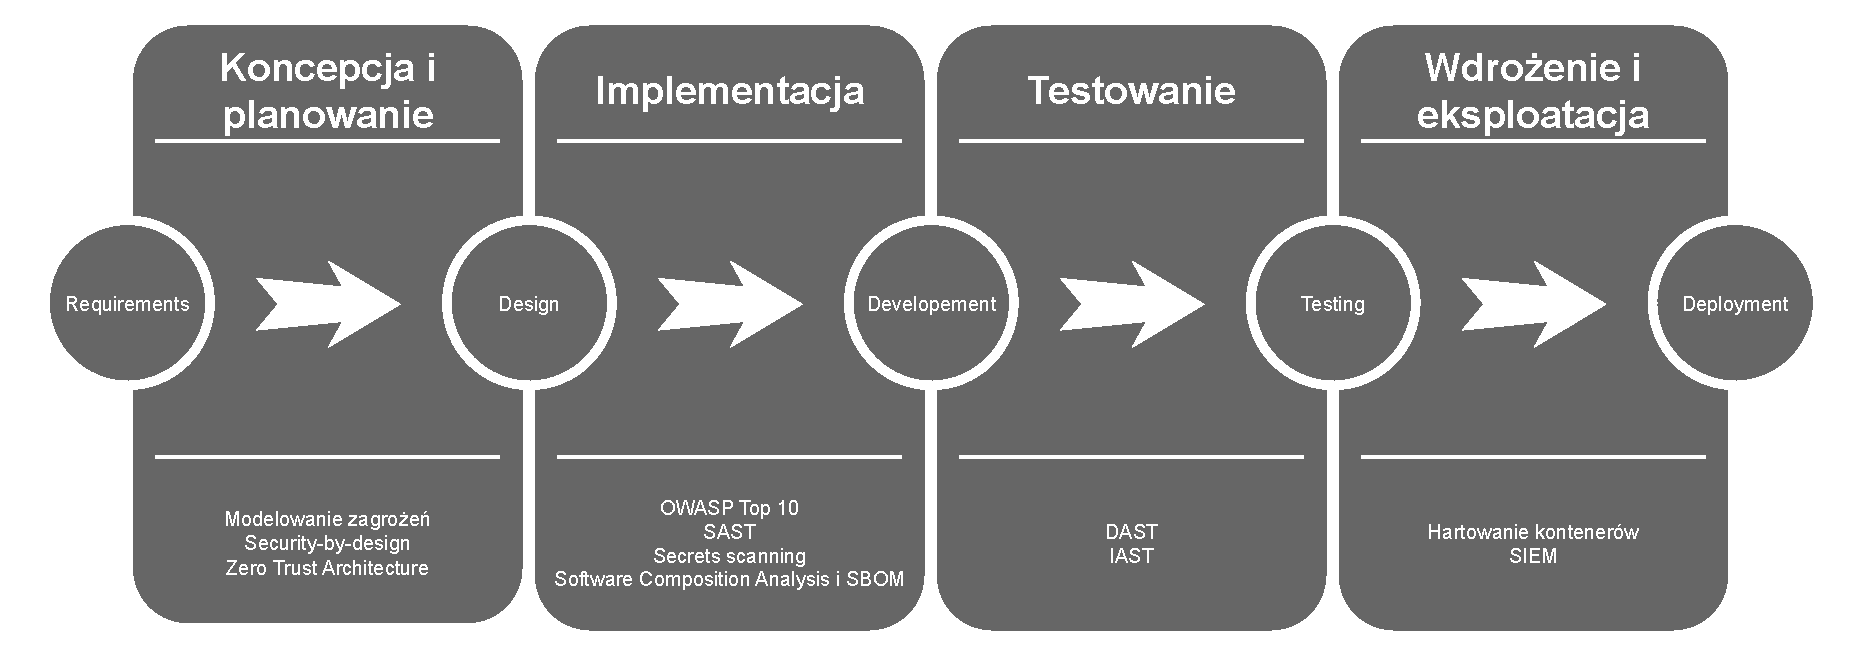
\includegraphics[width=10cm]{fig/ch12/SSDLC.pdf}
    \caption{Model Secure Software Development Life Cycle}
    \label{fig:ssdlc}
\end{figure}

\section{Faza koncepcji i planowania}

\subsection{Metodologie modelowania zagrożeń w praktyce}

Modelowanie zagrożeń stanowi punkt wyjścia dla bezpiecznego projektowania aplikacji. Cztery dominujące metodologie oferują różne podejścia do identyfikacji ryzyk:

\begin{itemize}

\item  STRIDE, zaproponowana przez Microsoft, klasyfikuje zagrożenia według sześciu kategorii:  spoofing (podszywanie się), tampering (modyfikacja), repudiation (zaprzeczenie), information disclosure (ujawnienie informacji), denial of service (odmowa usługi) i elevation of privilege (podniesienie uprawnień). Model ten pozwala identyfikować potencjalne zagrożenia na podstawie diagramów przepływu danych w systemie (Data Flow Diagrams, DFD). Microsoft Threat Modeling Tool to darmowe środowisko do tworzenia modeli opartych na STRIDE.~\footnote{~\url{https://msdn.microsoft.com/en-us/library/ee823878(v=cs.20).aspx}}

\item PASTA (Process for Attack Simulation and Threat Analysis)~\cite{UcedaVelez2015} to siedmiofazowa metodologia zorientowana na ryzyko biznesowe, opracowana przez Tony UcedaVelez i  Marco M. Morana w 2015 roku. Jej kluczową przewagą jest zgodność z celami organizacji oraz symulacja rzeczywistych scenariuszy ataku. PASTA jest rekomendowana dla dużych organizacji, systemów transakcyjnych wysokiej wartości oraz środowisk wymagających zgodności regulacyjnej.

\item LINDDUN~\cite{RoblesGonzalez2020} to ugruntowana metodologia modelowania zagrożeń prywatności, adresująca siedem kategorii: linkability (łączenie), identifying (identyfikacja), non-repudiation (niezaprzeczalność), detecting (wykrywanie), data disclosure (ujawnienie danych), unawareness (brak świadomości) oraz Non-compliance (Nieprzestrzeganie przepisów). Metodologia ta została opracowana przez ekspertów z KU Leuven i jest rekomendowana przez ENISA (Agencję Unii Europejskiej ds. Cyberbezpieczeństwa), a także referencjonowana w opisanym później NIST Privacy Framework.

\item CVSS (Common Vulnerability Scoring System)~\cite{First2019} to standardowa metoda oceny ryzyka oparta na liczbowej skali (0-10), stosowana do oceny wpływu i prawdopodobieństwa zagrożeń.

\item Attack Trees~\cite{Schneier1999} są narzędziem wizualnym, które pomaga zidentyfikować i zorganizować potencjalne ścieżki ataku, umożliwiając analizę skuteczności różnych metod obrony przeciwko tym zagrożeniom. Wizualizują one hierarchicznie ścieżki ataku z węzłami reprezentującymi cele i kroki. Metodologia wspiera analizę what-if dla oceny środków przeciwdziałania i jest często kombinowana z STRIDE oraz CVSS.
\end{itemize}

W tabeli~\ref{tab:threat_modeling_methods} pokazano porównanie wyżej wymienionych metodologii modelowania zagrożeń w oprogramowaniu pod względem 

\begin{table}[ht]
\centering
\caption{Porównanie metodologii modelowania zagrożeń w software}
\label{tab:threat_modeling_methods}
\begin{tabularx}{\textwidth}{*{3}{C}L}
\toprule
\textbf{Metodologia} & \textbf{Fokus} & \textbf{Złożoność} & \textbf{Najlepsze zastosowanie} \\
\midrule
STRIDE & Zagrożenia bezpieczeństwa & Niska-Średnia & Faza projektowania, zespoły początkujące \\
PASTA & Ryzyko biznesowe & Wysoka & Enterprise, compliance, priorytetyzacja ryzyka \\
LINDDUN & Prywatność & Średnia & GDPR/HIPAA, systemy przetwarzające dane osobowe (PII) \\
CVSS & Ocena i klasyfikacja podatności & Niska-Średnia & Ocena ryzyka luk, zarządzanie podatnościami \\
Attack Trees & Ścieżki i scenariusze ataku & Zmienna & Wizualizacja i analiza ścieżek ataku \\
\bottomrule
\end{tabularx}

\end{table}

\subsection{Zero Trust Architecture i Security-by-design}

NIST SP 800-207 to publikacja Narodowego Instytutu Standaryzacji i Technologii (NIST), która określa model Architektury Zero Trust (ZTA), promując zasadę "nigdy nie ufaj, zawsze weryfikuj"~\cite{NIST2020}. Definiuje ona siedem fundamentalnych zasad ZTA:

\begin{enumerate}
\item Wszystkie źródła danych i usługi obliczeniowe traktowane są jako zasoby.
\item Każda komunikacja jest zabezpieczona niezależnie od lokalizacji sieciowej.
\item Dostęp przyznawany jest per-sesja na podstawie dynamicznej polityki.
\item Ciągłe monitorowanie stanu bezpieczeństwa zasobów.
\item Ścisłe egzekwowanie uwierzytelniania i autoryzacji.
\item Kompleksowe logowanie i regularna okresowa ponowna ocena.
\end{enumerate}

Kluczowe komponenty obejmują Policy Decision Point (PDP) oceniający żądania dostępu, Policy Enforcement Point (PEP) jako punkt egzekwujący decyzję o dostępie oraz Policy Engine (PE) implementujący logikę decyzyjną. W kontekście aplikacji, ZTA realizuje się przez API gateways, service mesh oraz otwartego standardu SPIFFE (Secure Production Identity Framework for Everyone)~\footnote{~\url{https://spiffe.io/}} dla tożsamości usług.

Komplementarnym podejściem do ZTA jest inicjatywa CISA Secure by Design~\footnote{~\url{https://www.cisa.gov/securebydesign}}, promująca przeniesienie odpowiedzialności za bezpieczeństwo z użytkowników końcowych na producentów oprogramowania. Model ten opiera się na trzech fundamentalnych zasadach: przejęcie odpowiedzialności za wyniki bezpieczeństwa klientów, transparentność i rozliczalność  oraz budowa odpowiedniej struktury organizacyjnej i przywództwa. Deklaracja Secure by Designe definiuje siedem celów operacyjnych: zwiększenie adopcji wieloskładnikowego uwierzytelniania (MFA), redukcję domyślnych haseł, eliminację klas podatności, przyspieszenie instalacji poprawek, publikację polityk ujawniania podatności, dostarczanie rekordów CVE oraz wdrożenie mechanizmów wykrywania intruzów. Organizacje implementujące Secure by Design powinny traktować bezpieczeństwo jako wymóg na etapie projektowania, nie jako cechę dodawaną po wydaniu oprogramowania.

\section{Faza implementacji}

\subsection{OWASP Top 10 i wytyczne bezpiecznego kodowania}

OWASP Top 10~\footnote{~\url{https://owasp.org/Top10/}} to cyklicznie aktualizowany raport Open Web Application Security Project (OWASP), przedstawiającej dziesięć najważniejszych zagrożeń bezpieczeństwa dla aplikacji internetowych. Dokument ten służy jako standardowy punkt odniesienia dla programistów, testerów i firm, pomagając w identyfikacji krytycznych podatności na podstawie danych o ich powszechności, wykrywalności i wpływie. Lista OWASP Top 10 z 2021 pozostaje autorytatywną wersją z~zapowiedzianą publikacją wersji w tym roku (2025).

\subsection{Narzędzia analizy statycznej kodu źródłowego}

Analiza statyczna kodu źródłowego (Static Application Security Testing, SAST) ma na celu wykrywanie potencjalnych luk bezpieczeństwa, takich jak wstrzykiwanie SQL, podatności typu XSS, fałszowanie żądań po stronie serwera, niepoprawne użycie kryptografii, sekrety w kodzie źródłowym, niebezpieczne deserializacje i~inne. Dobra integracja narzędzi SAST w potoki ciągłej integracji umożliwia szybkie, powtarzalne i wczesne wykrywanie podatności w kodzie, skracając czas reakcji i obniżając koszty napraw.

W kontekście hipotetycznej firmy programistycznej wytwarzającej oprogramowanie głównie w technologii Microsoft .NET (C\#) oraz JavaScript/typeScript, korzystającej z systemu kontroli wersji git (Gitea/GitLab/Bitbucket) oraz systemów CI/CD (Jenkins/Gitlab Pipelines) kluczowe mogą być następujące czynniki wpływające na decyzję o użyciu narzędzi SAST: koszty licencji i utrzymania (preferowane darmowe OSS lub free tier), łatwość integracji z .NET i CI/CD (minimalna konfiguracja), jakość i pokrycie reguł dla C\#/.NET (OWASP Top 10, CVE, frameworki .NET) oraz innych stosowanych języków, wydajność skanowania (czas i zasoby w potokach), możliwość lokalnego uruchamiania (CLI/IDE) przez programistów (opcjonalne), wsparcie i aktywność projektu (community, aktualizacje reguł), zgodność licencyjna i bezpieczeństwo łańcucha dostaw (trusted images, SBOM). Następujące narzędzia SAST zaspokajają te czynniki:

\begin{itemize}
\item  Security Code Scan (SCS)~\footnote{~\url{https://security-code-scan.github.io}}. Charakterystyka: zestaw reguł Roslyn dla C\#/.NET, integracja jako pakiet NuGet/analyzer; działa w IDE, dotnet build i CI; OSS. Zalety: niski koszt (OSS), prosta integracja (NuGet), natychmiastowy feedback w IDE, reguły pod OWASP/CWE, łatwe egzekwowanie w CI (traktowanie ostrzeżeń jako błędy). Wady: brak aktualizacji (ostatnie wydanie ~2022), zgłoszone problemy ze zgodnością (.NET 8+), węższe pokrycie i mniejsze tempo aktualizacji reguł.
\item SonarQube/SonarCloud (reguły Security + Quality)~\footnote{~\url{https://www.sonarsource.com/open-source-editions/}}. Zalety: bogate raportowanie, reguły security i code quality, bramki jakości, integracje CI. Wady: koszt (pełne reguły security w edycjach płatnych), wymagany serwer (self-host) lub subskrypcja; dodatkowa konfiguracja.
\item Semgrep~\footnote{~\url{https://semgrep.dev/}}. Zalety: szybki, reguły konfigurowalne, darmowy core i darmowe reguły community, SARIF, łatwa integracja w CI, aktywnie rozwijany; wsparcie wielu języków i rodzajów plików (np. Dockerfile). Wady: część reguł wymaga dostrojenia pod kontekst projektu; pokrycie .NET stale rośnie, ale nie zawsze dorównuje narzędziom komercyjnym. 
\item Snyk~\footnote{~\url{https://snyk.io/}}. Zalety: Narzędzie typu all-in-one do SCA, SAST, CI/CD, kontenery. Wady: opłaty licencyjne, black-box (trudno konfigurowalny), mniejsza liczba reguł SAST
\end{itemize}

\subsection{Secrets scanning}

Wykrywanie wycieków sekretów w kodzie źródłowym jest ważnym elementem bezpiecznego DevSecOps, zapobiegającym przypadkowemu ujawnianiu kluczy API, haseł czy tokenów w repozytoriach Git. Wielowarstwowe podejście z narzędziami takimi jak Gitleaks czy TruffleHog pozwala na szybkie wykrywanie i blokowanie wysyłania zmian, minimalizując ryzyko wykorzystania luk bezpieczeństwa.

Narzędzia do skanowania sekretów w kodzie źródłowym:

\begin{itemize}
\item Gitleaks~\footnote{~\url{https://gitleaks.io/}}. Najlepsze wyniki w wielu benchmarkach dzięki szybkości i~niskim poziomie fałszywych alarmów. Jest szybki, lekki i dobrze nadaje się do CI/CD.

\item TruffleHog~\footnote{~\url{https://trufflesecurity.com/}}. Oferuje entropy analysis + pattern matching oraz skanowanie rpozytoriów Git, S3 buckets, Confluence, Slack i innych. 

\item GitGuardian~\footnote{~\url{https://www.gitguardian.com/}}. Bezpłatny bazujący na CLI ggshield dla indywidualnych użytkowników oraz komercyjna platforma dashboardem i validity checks.

\item GitHub Secret Scanning~\footnote{~\url{https://docs.github.com/en/code-security/secret-scanning}}. Skanuje kod w poszukiwaniu sekretów i zapewnia push protection – blokowanie prób wysłania wrażliwych danych do repozytorium. W przypadku wykrycia tokenu GitHub powiadamia odpowiedniego dostawcę w celu jego unieważnienia. 

\item GitLab Secret Detection~\footnote{~\url{https://docs.gitlab.com/user/application_security/secret_detection/}} wykorzystuje wewnętrznie Gitleaks z opcją Secret Push Protection.
\end{itemize}

\subsection{Software Composition Analysis i SBOM}

Software Composition Analysis (SCA) oraz Software Bill of Materials (SBOM) umożliwiają identyfikację i zarządzanie komponentami open source w aplikacjach, minimalizując ryzyka podatności i naruszeń licencyjnych w łańcuchu dostaw oprogramowania~\cite{Prana2021}. Formaty SBOM:
\begin{itemize}
\item SPDX (ISO/IEC 5962:2021) to międzynarodowy standard oferujący kompleksowe metadane skupione na zgodności licencyjnej oprogramowania.
\item SPDX 3.0 wydany w kwietniu 2024, wprowadza specjalizowane profile ułatwiające zastosowanie standardu w konkretnych przypadkach użycia, takich jak bezpieczeństwo, kompilacja oprogramowania, sztuczna inteligencja oraz zestawy danych.
\item CycloneDX (OWASP) to format SBOM o priorytecie bezpieczeństwa, oferujący natywne wsparcie dla VEX (Vulnerability Exploitability eXchange) do oceny podatności, podpisy cyfrowe dla integralności oraz identyfikację komponentów poprzez Package-URL (PURL).
\end{itemize}

Narzędzia generujące SBOM:
\begin{itemize}
\item Syft~\footnote{~\url{https://anchore.com/platform/sbom/}} biblioteka Go i narzędzie CLI do generowania CycloneDX/SPDX, zawiera CPE (Common Platform Enumeration).
\item Trivy~\footnote{~\url{https://www.aquasec.com/products/trivy/}} to wszechstronny skaner all-in-one do wykrywania podatności, błędów konfiguracji, sekretów oraz generowania SBOM.
\item cdxgen~\footnote{~\url{https://owasp.org/www-project-cdxgen/}} oficjalny generator CycloneDX od OWASP; posiada profile dla różnych przypadków użycia.
\end{itemize}

\section{Faza testowania}

Faza testowania w procesie bezpiecznego wytwarzania oprogramowania koncentruje się na zautomatyzowanych metodach wykrywania podatności bezpieczeństwa (DAST i IAST), które można wbudować w potok ciągłej integracji i dostarczania~\cite{Abdiukov2024}. 

Świadomie pominięto tutaj zagadnienia związane z testami penetracyjnymi (penetration testing) oraz testowaniem fuzz (fuzz testing), które mimo istotnej roli w ocenie bezpieczeństwa wykraczają poza zakres zautomatyzowanych mechanizmów kontroli możliwych do wdrożenia w standardowych procesach deweloperskich. Testy penetracyjne wymagają specjalistycznej wiedzy i są zazwyczaj są przeprowadzane okresowo przez dedykowane zespoły, podczas gdy fuzz-testing, choć możliwy do zautomatyzowania, stanowi wysoce wyspecjalizowaną dziedzinę wymagającą odrębnego omówienia.

\subsection{DAST}

DAST (Dynamic Application Security Testing) to testowanie bezpieczeństwa typu black-box działającej aplikacji, symulujące rzeczywiste ataki zewnętrznego napastnika bez dostępu do kodu źródłowego. Metoda ta identyfikuje podatności w~środowisku wykonawczym takie jak XSS, SQL injection czy błędy konfiguracji, idealnie integrując się z CI/CD. Narzędzia DAST:

\begin{itemize}
\item OWASP ZAP~\footnote{~\url{https://www.zaproxy.org/}} to najpowszechniej używany skaner z funkcjami Spider Module, AJAX Spider (headless Chromium), Active/Passive Scanning oraz API Scanning (OpenAPI/Swagger). Integracja CI/CD przez obraz Dockera, plugin do Jenkinsa lub GitHub Actions. 

\item Burp Suite DAST~\footnote{~\url{https://portswigger.net/burp/dast}} oferuje skanowanie oparte na przeglądarce, testowanie bezpieczeństwa poza OAST (Out-of-band Application Security Testing), ponad 250 rozszerzeń oraz skalowalne skanowanie wielu aplikacji jak również wsparcie dla uwierzytelniania wieloskładnikowego (MFA), wersję hostowaną w chmurze oraz skanowanie podatności w~protokole WebSocket.

\item Nuclei~\footnote{~\url{https://projectdiscovery.io/nuclei}} to skaner oparty na szablonach prowadzony przez społeczność (w~tym wiele szablonów dla CVE). Oferuje mniej fałszywych alarmów dzięki symulacji warunków rzeczywistych. Posiada aktualizacje społecznościowe. Obsługiwane protokoły: HTTP, DNS, TCP, SSL, WHOIS, JavaScript.
\end{itemize}

\subsection{IAST}

IAST (Interactive Application Security Testing) to hybrydowa metoda testowania bezpieczeństwa, instrumentująca aplikację sensorami w runtime, co łączy analizę statyczną kodu z dynamicznym monitorowaniem przepływu danych i wykonania podczas interaktywnych testów. Ma zapewniać wyższą precyzję przez kontekst na poziomie kodu w środowiskach CI/CD i QA. Wymaga integracji z aplikacją (Java, .NET, Node.js itp.).

\begin{itemize}
    \item OWASP Noir~\footnote{~\url{https://owasp.org/www-project-noir/}} narzędzie IAST wspomagające DAST poprzez statyczną analizę kodu źródłowego.

\item Contrast Security~\footnote{~\url{https://www.contrastsecurity.com/glossary/interactive-application-security-testing}} oferuje instrumentację agentową zwiększając wskaźnik wykrywlności. Wspiera Java, .NET, Node.js, Python, Ruby, Go.

\item Black Duck Seeker~\footnote{~\url{https://www.blackduck.com/interactive-application-security-testing.html}} rozwiązanie z aktywną weryfikacją i śledzeniem danych wrażliwych dla aplikacji webowych, automatyzujące testy bezpieczeństwa dla zespołów deweloperskich.
\end{itemize}

\section{Faza wdrożenia i eksploatacji}

Faza wdrożenia i eksploatacji stanowi moment, w którym aplikacja trafia do środowiska produkcyjnego i staje się dostępna dla użytkowników końcowych oraz potencjalnych napastników.

\subsection{Hartowanie kontenerów}

Obrazy kontenerów mogą zawierać podatności w bibliotekach i zależnościach, znane luki bezpieczeństwa (CVE) w obrazach bazowych, przypadkowo osadzone sekrety (klucze API, hasła, tokeny) oraz błędy konfiguracji. Hartowanie kontenerów (conainter hardening) zapewnia systematyczne skanowania podatności w~kontenerach

Narzędzia takie jak Trivy (opisany w skecji dotyczącej SBOM) oferują kompleksową analizę obejmującą wykrywanie podatności w zależnościach dla ponad 20 menedżerów pakietów (w tym npm, yarn, NuGet), detekcję wycieków sekretów, analizę plików Dockerfile oraz generowanie SBOM w~formatach SPDX i~CycloneDX, integrując się natywnie z potokami CI/CD i rejestrami obrazów.

Bezpieczeństwo kontenerów w środowisku produkcyjnym rozciąga się również na warstwę orkiestracji, gdzie Kubernetes wprowadza dedykowane mechanizmy kontroli w postaci Pod Security Standards (PSS)~\footnote{~\url{https://kubernetes.io/docs/concepts/security/pod-security-standards/}}. Egzekwowanie polityk bezpieczeństwa na poziomie klastra realizowane jest przez silniki takie jak OPA/Gatekeeper wykorzystujący język Rego dla złożonych reguł lub Kyverno oferujący prostszą składnię opartą na natywnym YAML, zapewniając automatyczną weryfikację zgodności wdrażanych zasobów z organizacyjnymi standardami bezpieczeństwa.

\subsection{SIEM}

Monitoring bezpieczeństwa i zarządzanie incydentami (Security information and event management, SIEM) tworzą zamknięty cykl wykrywania, analizy i remediacji zagrożeń poprzez analizę w czasie rzeczywistym alertów bezpieczeństwa generowanych przez aplikacje i sprzęt sieciowy. Rozwiązania typu SIEM:

\begin{itemize}
\item Splunk Enterprise Security~\footnote{\url{https://www.splunk.com/en_us/products/enterprise-security.html}} ma ponad 1500 integracji, zaawansowana naliza, język zapytań SPL
\item Microsoft Sentinel~\footnote{~\url{https://www.microsoft.com/pl-pl/security/business/siem-and-xdr}} jest zbudowany dla ekosystemu chmurowego Azure, wykrywanie zagrożeń oparte o AI/ML, język zapytań KQL
\item Elastic Security~\footnote{~\url{https://www.elastic.co/security}}: integracja ze stackiem ELK, wysoce skalowalny, otwartoźródłowy
\item Wazuh~\footnote{~\url{https://wazuh.com/}}: Open source, schematy zgodności z HIPAA/PCI-DSS, mozliwość dosotoswania do potrzeb
\end{itemize}

\section{Wnioski i dalsze kroki}

Skuteczna implementacja Secure Software Development Life Cycle w organizacjach deweloperskich wymaga zbalansowanego podejścia łączącego automatyzację z ekspertyzą ludzką. Strategia shift-left security~\cite{Malik2025} realizowana przez integrację narzędzi SAST/SCA w potokach CI/CD (Semgrep, Snyk, Security Code Scan, Gitleaks) umożliwia wczesne wykrywanie podatności przy minimalnym wpływie na przepustowość zespołów deweloperskich. Wielowarstwowa ochrona sekretów stanowi fundament dla zapobiegania wyciekom danych uwierzytelniających. SBOM jako ciągła praktyka wymaga utrzymywania SBOM zsynchronizowanego z rzeczywistym stanem zależności w produkcji. 

Przyszłe prace powinny skupić się na trzech kluczowych obszarach wymagających pogłębionej analizy empirycznej i rozwiązań technologicznych:

\begin{itemize}
\item Wspomagana AI Security Code Review i wykrywanie podatności w~oparciu o modele językowe.
\item Zautomatyzowane testowanie bezpieczeństwa dla architektur cloud-native.
\item Weryfikacja bezpieczeństwa łańcucha dostaw.
\end{itemize}

\begin{thebibliography}{30}

\bibitem{Pochu2024}
Pochu S., Kathram S.R.,
Integrating Security Requirements Into Software Development: A Comprehensive Approach to Secure Software Design,
Journal for Multidisciplinary Research, Vol. 1, No. 03, 60--76 (2024).

\bibitem{Verizon2025}
Verizon,
2025 Data Breach Investigations Report,
Verizon Business, https://www.verizon.com/business/resources/reports/dbir/ (2025).

\bibitem{BlackDuck2025}
Black Duck,
The Global State of DevSecOps: Balancing AI Usage and Risk in 2025,
Black Duck Software, Inc., 
https://www.blackduck.com/content/dam/black-duck/en-us/reports/rep-global-devsecops-report.pdf (2025).

\bibitem{UcedaVelez2015}
UcedaVelez T., Morana M.M.,
Risk Centric Threat Modeling: Process for Attack Simulation and Threat Analysis,
Wiley Publishing (2015).

\bibitem{RoblesGonzalez2020}
Robles-González A., Parra-Arnau J., Forné J.,
A LINDDUN-Based framework for privacy threat analysis on identification and authentication processes,
Computers \& Security, Vol. 94, 101755 (2020).

\bibitem{Schneier1999}
Schneier B.,
Attack Trees,
Dr. Dobb's Journal, 
https://www.schneier.com/academic/archives/1999/12/attack\_trees.html (December 1999).

\bibitem{First2019}
FIRST (Forum of Incident Response and Security Teams),
Common Vulnerability Scoring System: Specification Document,
FIRST.org (2019).

\bibitem{NIST2020}
Rose S., Borchert O., Mitchell S., Connelly S.,
Zero Trust Architecture,
NIST Special Publication 800-207,
doi: 10.6028/NIST.SP.800-207,
National Institute of Standards and Technology (August 2020).

\bibitem{Prana2021}
Prana G.A.A., Sharma A., Shar L.K., Foo D., Santosa A.E., Sharma A., Lo D.,
Out of sight, out of mind? How vulnerable dependencies affect open-source projects,
Empirical Software Engineering, Vol. 26, No. 4, 59,
doi: 10.1007/s10664-021-09959-3 (2021).

\bibitem{Abdiukov2024}
Abdiukov T.,
Automated security testing in DevSecOps pipelines: Integrating AI-based vulnerability discovery and compliance validation,
World Journal of Advanced Research and Reviews, Vol. 22, No. 01, 2083--2093,
doi: 10.30574/wjarr.2024.22.1.1083 (2024).

\bibitem{Malik2025}
Malik G., Prashasti P.,
Shift Left Security,
The Eastasouth Journal of Information System and Computer Science, Vol. 2, No. 03, 219--245,
doi: 10.58812/esiscs.v2i03.528 (2025).

\end{thebibliography}

\chapterauthor{Krzysztof Stępniak}
\chapter[Środki organizacyjne \ldots]{Środki organizacyjne i techniczne ograniczające zagrożenia powodowane przez homoglify w URL}
\label{intro} % Always give a unique label
% use \chaptermark{}
% to alter or adjust the chapter heading in the running head

\thispagestyle{empty}
\vspace{-8mm} {\large Krzysztof Stępniak} \vspace{8mm}

\section{Wprowadzenie}
Współczesne funkcjonowanie społeczeństwa w coraz większym stopniu opiera się na usługach sieciowych, a systemy komputerowe towarzyszą użytkownikom w niemal wszystkich obszarach codziennej aktywności. Komunikacja międzyludzka uległa znaczącej cyfryzacji i w dużej mierze została przeniesiona do środowiska internetowego. W celu ułatwienia nawigacji w złożonej ujednoliconej przestrzeni identyfikatorów zasobów (URI)~\footnote{~RFC3986~\url{https://datatracker.ietf.org/doc/html/rfc3986}} usług cyfrowych opracowano system DNS, oparty na hierarchicznej strukturze nazw domen, które są łatwe do zapamiętania oraz intuicyjnie kojarzone z określonymi usługami lub podmiotami.


\begin{equation} \label{eq12.1:Schemat URI} 
%\[
\text{URI} \;=\;
\underbrace{\text{scheme}}_{\text{schemat}}
\;:://\;
\underbrace{\text{userinfo}}_{\substack{\text{informacje o} \\ \text{użytkowniku}}}
@\!
\underbrace{\text{host}}_{\substack{\text{nazwa} \\ \text{hosta}}}
.\!
\underbrace{\text{domain}}_{\text{domena}}
:\!
\underbrace{\text{port}}_{\text{port}}
/\!
\underbrace{\text{path}}_{\text{ścieżka}} \\
%\]
\end{equation}
%\noindent\text{Schemat URI \eqref{eq:example}}

Z czasem jednak pojawiły się nadużycia wynikające z podatności ludzkiej percepcji wzrokowej na manipulacje wyglądem adresów URL. Atak homograficzny to jedna z technik przeprowadzania tego schematu. Homograf to litera lub ciąg znaków, który wizualnie można pomylić z inną literą lub ciągiem znaków. Na przykład, używając większości czcionek bezszeryfowych, łacińska litera l (mała litera "L") jest wizualnie podobna z łacińską literą I (wielka litera "i"). Poniższe znaki, renderowane w ten sposób, przy użyciu takiej czcionki, są mylone, jeśli nie nieodróżnialne~\cite{Holgers2006}:
\[
\text {http://www.paypal.com} \;\; \text{vs.}\;\; \text{http://www.paypaI.com} \;\; 
\] % TODO:zmienic czcionke na bezszeryfowa, moze Arial?
W ten sposób można było przygotować kampanię phishingową\footnote{~Phishing~\url{https://www.cisa.gov/uscert/ncas/tips/ST04-014}}, w której korespondencja elektroniczna z odpowiednio spreparowanym takim adresem w~hiperłączu uwiarygodnionym certyfikatem SSL zachęci użytkownika do podania swoich danych logowania w docelowej podrobionej witrynie graficznie nieodbiegającej od oryginału.

Problem ten uległ dodatkowej intensyfikacji wraz z wprowadzeniem do przestrzeni identyfikatorów międzynarodowych nazw domen (ang. IDN\footnote{~IDN~Internationalized Domain Names \url{https://datatracker.ietf.org/doc/html/rfc5890}}) internetowych znaków narodowych w standardzie Unicode, które znacząco poszerzyły możliwości tworzenia wizualnie podobnych, lecz fałszywych nazw domen. Na przestrzeni wielu narodowych alfabetów występują glify o podobnym wyglądzie, choćby dla powyższego przykładu łacińska mała litera p (Unicode U+0070) odpowiada wizualnie literze p w cyrylicy, która jest tam małą literą "r" (Unicode U+0440)\cite{Holgers2006}.
%\[
%\text {0077 0077 0077 002E 0070 0061 0079 0070 0061 006C 002E 0063 006F 006D} \;\; %\text{vs.}\;\; \text{http://www.paypaI.com} \;\; 
%\] % TODO:zmienic czcionke na bezszeryfowa, moze Arial?

Dotychczasowe działania z zakresu podnoszenia świadomości zagrożeń phishingowych koncentrowały się przede wszystkim na edukowaniu użytkowników w~zakresie identyfikacji obecności oraz analizy zawartości certyfikatów SSL potwierdzających tożsamość i wiarygodność odwiedzanej strony internetowej. Współcześnie jednak nie istnieją techniczne ograniczenia uniemożliwiające uzyskanie takich certyfikatów również dla domen wykorzystujących homoglify, co znacząco obniża skuteczność tradycyjnych mechanizmów weryfikacji wiarygodności witryn. 
Z uwagi na to, że system DNS technicznie akceptuje tylko ograniczony zestaw znaków ASCII wprowadzono standaryzowane w RFC 3492~\footnote{~RFC3492~\url{https://datatracker.ietf.org/doc/html/rfc3492}} rozszerzenie o nazwie Punycode, które stało się kluczową częścią systemu IDN, umożliwiając globalne rozszerzenie nazw domen poza standardowe znaki łacińskie.

%Wielu popu
Celem tego badania jest przegląd środków organizacyjnych i technicznych mających na celu ograniczenie zagrożeń bezpieczeństwa powodowanych przez homoglify Unicode i znaki wizualnie trudne do odróżnienia.

%\label{sec:1}
%tekst
\section{Przegląd literatury}
Literatura na temat łagodzenia wpływu homoglifów obejmuje różnorodne podejścia metodologiczne, począwszy od głębokiego uczenia po implementacje oparte na przeglądarce.


\begin{table}[ht]
\centering
\caption{Charakterystyka uwzględnionych badań}
\label{tab:badaniaTab}
{\footnotesize
\begin{tabularx}{\textwidth}{p{1.75cm}p{2.5cm}p{4cm}L}
\bottomrule
\textbf{Badanie} & \textbf{Typ badania} & \textbf{Główny nurt} & \textbf{Kontekst docelowy} \\ \midrule
Hang Hu, 2021  &  analiza empiryczna i badanie użytkowników  & Ocena obrony na poziomie przeglądarki & Homografie IDN \\ 
Johnny Al Helou, 2010  & Nie określono & Obrona wizualna po stronie klienta & IDN z alfabetem innym niż łaciński (arabski) \\ 
Hiroaki Suzuki, 2019  & Badanie pomiarowe na dużą skalę & Zautomatyzowany framework wykrywania & Ataki homograficzne IDN z wykorzystaniem Unicode \\ 
P. Hannay, 2012  & Ankieta & Badanie strategii łagodzenia & wizualne podobieństwo IDN \\ 
Tobias Holgers, 2006  & Badanie pomiarowe & ilościowe określenie rozpowszechnienia ataków & IDN i homografy znaków łacińskich \\ 
Florian Quinkert, 2019  & Badanie pomiarowe & Wykrywanie i monitorowanie domen homograficznych & Znaki IDN i Unicode o podobnym wyglądzie \\ 
R. Yazdani, 2020  & Badanie pomiarowe & Wykrywanie podejrzanych domen za pomocą DNS & Podobieństwo wizualne IDN i Unicode \\ 
Tyson McElroy, 2017  & Kontrolowany eksperyment & Ocena strategii łagodzenia zagrożeń przeglądarek & Ataki IDN o mieszanym skrypcie \\ 
J. Abawajy, 2017  & Kontrolowany eksperyment lub studium przypadku & Obrona z dodatkami do przeglądark & Ataki homograficzne IDN \\ 
Yuta Sawabe, 2019 & Kontrolowany eksperyment & Metoda wykrywania oparta na OCR & Podobieństwo wizualne w domenach IDN \\ \bottomrule
\end{tabularx}
}

\end{table}


Uwzględnione badania obejmują lata 2006–2021 i odzwierciedlają ewolucję badań nad atakami homograficznymi na przestrzeni 15 lat. Korpus obejmuje cztery badania pomiarowe badające rozpowszechnienie ataków i~możliwości ich wykrywania \cite{Suzuki2019}, trzy kontrolowane eksperymenty oceniające konkretne metody ograniczania ryzyka \cite{McElroy2017} oraz dwa badania ankietowe badające mechanizmy obronne na poziomie przeglądarki \cite{Hu2021}. Wszystkie badania dotyczą zagrożeń związanych z homoglifami związanymi z domenami międzynarodowymi (IDN), przy czym większość z nich koncentruje się na technicznych środkach zaradczych, a nie na politykach organizacji.

\section{Środki techniczne}
\begin{table*}[h]
\centering
\caption{Środki techniczne}
\label{tab:techniczneTab}
{\footnotesize
\begin{tabularx}{\textwidth}{LLp{4cm}L}
\toprule
\textbf{Podejście do minimalizacji ryzyka} & \textbf{Poziom wdrożenia} & \textbf{
Kluczowe mechanizmy} & \textbf{Badania} \\ \midrule
Zasady dotyczące nazw domen (IDN) w przeglądarce  &  strona klienta  & Testowanie polityki typu „czarna skrzynka” przy użyciu zautomatyzowanych narzędzi & Hang Hu et al., 2021 \\
Wyświetlanie Punycode  & strona klienta & Wyświetlanie znaków Unicode w formacie ASCII & McElroy et al., 2017; Al Helou et al., 2010 \\ 
Kodowanie kolorami alfabetu  & strona klienta & Wizualne różnicowanie typów pisma & McElroy et al., 2017 \\ 
Domena na białej liście  & strona klienta /rejestrator domeny & Dopuszczanie tylko domen wstępnie zatwierdzonych & Al Helou et al., 2010; McElroy et al., 2017 \\ 
Framework ShamFinder & system detekcji & Zautomatyzowana konstrukcja bazy danych homoglifów & Suzuki et al., 2019 \\ 
Wykrywanie oparte na OCR  & system detekcji & Wizualne rozpoznawanie podobieństw & Sawabe et al., 2019 \\ 
Wykrywanie oparte na DNS  & strona serwera/sieć & Aktywne pomiary DNS za pośrednictwem OpenINTEL & Yazdani et al., 2020 \\ 
Rozszerzenie tabeli homoglifów  & system detekcji & Rozszerzone tabele możliwości pomyłki Unicode & Yazdani et al., 2020 \\ 
Dodatek do przeglądarki  & strona klienta & Automatyczne zapobieganie atakom bez zmiany interakcji użytkownika & Abawajy et al., 2017 \\ 
Wstępne pobieranie miniatur & strona klienta & Wizualna weryfikacja stron internetowych & Al Helou et al., 2010 \\ \bottomrule
\end{tabularx}
}

\end{table*}


Ochrona realizowana na poziomie przeglądarki stanowi najlepiej przebadaną kategorię technicznych środków zaradczych. Główny mechanizm polega na wyświetlaniu znaków Unicode w formacie Punycode w celu ujawnienia ich reprezentacji w kodzie ASCII \cite{McElroy2017}. Wiele przeglądarek wdrożyło to podejście, w tym już Internet Explorer 7 \cite{McElroy2017} i Mozilla Firefox, z zaktualizowanymi algorytmami sprawdzającymi kombinacje skryptów. Kodowanie kolorami skryptów zapewnia dodatkową wizualną wskazówkę umożliwiającą rozróżnianie zestawów znaków \cite{McElroy2017}.

Podejścia skoncentrowane na wykrywaniu pojawiły się jako środki uzupełniające. Framework ShamFinder zapewnia automatyczne wykrywanie poprzez automatyczną budowę baz danych homoglifów \cite{Suzuki2019}, podczas gdy Yazdani et al. rozszerzyli istniejące tabele homoglifów Unicode, aby poprawić możliwości wykrywania \cite{Yazdani2020}. Sawabe et al. zaproponowali innowacyjne podejście oparte na OCR, które wykorzystuje rozpoznawanie podobieństwa wizualnego do automatycznego wykrywania homograficznych nazw domen (IDN) \cite{Sawabe2019}, rozwiązując ograniczenia predefiniowanych metod mapowania.

\section{Polityki organizacyjne i strategie obronne}
Najbardziej kompleksowe omówienie polityk organizacyjnych, proponując dwutorową strategię obronną dla właścicieli domen przedstawiono w \cite{Quinkert}. Podejście to obejmuje identyfikację i prewencyjną rejestrację powszechnie stosowanych substytucji znaków, w połączeniu z ciągłym monitorowaniem pod kątem złośliwych rejestracji. W przypadku naruszenia znaku towarowego właściciele domen mogą skorzystać z istniejących mechanizmów rozwiązywania konfliktów, aby zażądać przeniesienia własności domen homograficznych.

\section{Kontekst implementacyjny}

\begin{table*}[!ht]
\centering
\caption{Kontekst implementacyjny}
\label{tab:implementacyjnyTab}
{\footnotesize
\begin{tabularx}{\textwidth}{LLp{3cm}p{4cm}}
\toprule
\textbf{Badanie} & \textbf{Platforma technologiczna} & \textbf{
Poziom wdrożenia} & \textbf{Rozważania skalowalności} \\ \midrule
Hang Hu et al., 2021  &  Chrome, Firefox, Safari, Edge, IE, mobile browsers  & Strona klienta &Ponad 9000 przypadków testowych \\ 
Al Helou et al., 2010  & Nie określono & Strona klienta & Rozwiązania zaprojektowane tak, aby były dyskretne i łatwe do wdrożenia \\ 
P. Hannay et al., 2012  & Przeglądarki internetowe, klienci poczty e-mail & Strona klienta &Wiele aplikacji powoli się wdraża \\ 
Holgers et al., 2006  & Przeglądarki, systemy DNS & Przeglądarki, systemy DNS & Nie określono \\ 
Quinkert et al., 2019 & Domainlists.io, rozproszony crawler & Mechanizm wykrywania & Rozproszony crawler do przetwarzania na dużą skalę \\ 
Yazdani et al., 2020  & system detekcji & Wizualne rozpoznawanie podobieństw & Sawabe et al., 2019 \\ 
McElroy et al., 2017  & strona serwera/sieć & Aktywne pomiary DNS za pośrednictwem OpenINTEL & Yazdani et al., 2020 \\ 
Abawajy et al., 2017  & system detekcji & Rozszerzone tabele możliwości pomyłki Unicode & Yazdani et al., 2020 \\ \bottomrule
\end{tabularx}
}

\end{table*}


Wdrożenia realizowane po stronie klienta dominują w obecnym krajobrazie implementacyjnym, a mechanizmy obronne oparte na przeglądarce stanowią podstawowy komponent warstwy ochronnej \cite{Hu2021}. Na tym tle podejście zaproponowane przez Yazdaniego et al. wyróżnia się wykorzystaniem pomiarów DNS prowadzonych po stronie serwera z użyciem platformy OpenINTEL, która wykonuje codziennie migawki obejmujące ponad 65\% przestrzeni nazw DNS \cite{Yazdani2020}.

Istotną barierą dla skutecznej ochrony jest powolne wdrażanie strategii łagodzenia przez aplikacje \cite{Hannay2011}. Skuteczność zabezpieczeń na poziomie przeglądarki jest dodatkowo ograniczona przez zachowania użytkowników związane z aktualizacjami, ponieważ tempo wprowadzania nowych wersji przeglądarek bezpośrednio wpływa na narażenie na luki w zabezpieczeniach~\cite{McElroy2017}.

\section{Dowody skuteczności} %Effectiveness Evidence}
\begin{table*}[!ht]
\centering
\caption{Wyniki skuteczności}
\label{tab:skutecznościTab}
{\footnotesize
\begin{tabularx}{\textwidth}{p{1.5cm}LLp{3cm}}
\toprule
\textbf{Badanie} & \textbf{Wyniki ilościowe} & \textbf{
Ocena skuteczności} & \textbf{Zidentyfikowane ograniczenia} \\ \midrule
Hang Hu et al., 2021  &  Oceniono ponad 9000 przypadków testowych  & Wszystkie testowane przeglądarki mają słabe punkty w regułach &Przeglądarka Chrome zmieniła zasady, aby ponownie zezwolić na używanie niektórych homografów \\ 
Suzuki et al., 2019  & Przeprowadzono pomiary na dużą skalę & Framework zapewnia skuteczne środki zaradcze & Nie zgłoszono żadnych konkretnych wskaźników ilościowych \\ 
Quinkert et al., 2019  & Wykryto \~3000 domen homograficznych; >200 domen oszustw pominiętych przez narzędzia branżowe & Wykrywa złośliwe domeny szybciej niż VirusTotal/Google Safe Browsing & Rejestracja prewencyjna wszystkich wariantów homograficznych jest niemożliwa \\ 
Yazdani et al., 2020  & 2,97× poprawa wykrywania w porównaniu z istniejącymi tabelami & Proaktywne wykrywanie zapewnia wczesne alerty & Opiera się na rozszerzonych tabelach homoglifów \\ 
McElroy et al., 2017 & Przetestowano wiele wersji przeglądarek (2011–2017) & Wysoka skuteczność łagodzenia skutków za pomocą wielu alfabetów; brak łagodzenia skutków za pomocą jednego alfabetu & W wersji Firefoksa brakowało funkcji łagodzących \\ 
Abawajy et al., 2017  & Implementacja zademonstrowana jako dodatek & Skuteczny, bez zauważalnych kosztów dodatkowych & Nie podano danych ilościowych \\
Sawabe et al., 2019  & Oceniono na podstawie 3,19 mln prawdziwych nazw domen IDN i 10 000 złośliwych nazw domen IDN & Metoda OCR wykrywa homografy, których nie wykrywają konwencjonalne metody & Nie określono \\ \bottomrule
\end{tabularx}
}

\end{table*}

Wyniki ilościowe wskazują na zróżnicowany poziom skuteczności różnych podejść. Yazdani et al. osiągnęli 2,97-krotną poprawę w wykrywaniu domen homograficznych w porównaniu z istniejącymi tabelami pomyłek \cite{Yazdani2020}. Mechanizm detekcji Quinkerta et al. zidentyfikował około 3000 domen kandydujących i ponad 200 domen oszustw, które nie zostały wykryte przez obecne narzędzia branżowe, takie jak VirusTotal i Google Safe Browsing \cite{Quinkert}.

Obrona na poziomie przeglądarki przynosi mieszane rezultaty. McElroy et al. stwierdzili wysoką skuteczność w łagodzeniu zagrożeń związanych z wieloma alfabetami w różnych rodzajach przeglądarek \cite{McElroy2017}, przy czym Opera i Chromium wykazały się szczególnie silnym wykrywaniem mieszanych alfabetów\cite{McElroy2017}. Jednak wszystkie testowane przeglądarki wykazywały słabości w swoich regułach obronnych \cite{Hu2021}, a badania użytkowników potwierdziły, że homograficzne domeny IDN omijające zabezpieczenia przeglądarek pozostają wysoce zwodnicze dla użytkowników \cite{Hu2021}.

\section{Zidentyfikowane ograniczenia i luki}

\begin{table*}[!ht]
\centering
\caption{Zidentyfikowane ograniczenia i luki}
\label{tab:ograniczeniaTab}
{\footnotesize
\begin{tabularx}{\textwidth}{Lp{5cm}L}
\toprule
\textbf{Kategoria ograniczenia} & \textbf{Konkretne kwestie} & \textbf{
Badania} \\ \midrule
Ograniczenia techniczne  &  Wszystkie przeglądarki mają słabe punkty w regułach\cite{Hu2021}; Chrome cofnął zasady\cite{Hu2021};W wersji Firefoksa brakowało rozwiązań łagodzących\cite{McElroy2017}  & Hang Hu et al., 2021; McElroy et al., 2017 \\
Luki w pokryciu  & Niezaadresowane ataki oparte na pojedynczym alfabecie\cite{McElroy2017}; konwencjonalne metody nie są w stanie wykryć niezdefiniowanych znaków\cite{Sawabe2019}; istniejące tabele homoglifów są niewystarczające\cite{Yazdani2020} & McElroy et al., 2017; Sawabe et al., 2019; Yazdani et al., 2020  \\ 
Ograniczenia skalowalności  & Wymagane ręczne aktualizacje mapowania\cite{Sawabe2019}; prewencyjna rejestracja wszystkich wariantów niewykonalna\cite{Quinkert} & Sawabe et al., 2019; Quinkert et al., 2019  \\ 
Podatność użytkownika  & Homografy omijające obronę pozostają wysoce mylące & Hang Hu et al., 2021  \\ 
Bariery adopcyjne & Powolne wdrażanie przez aplikacje\cite{Hannay2011}; biała lista zachowana wyłącznie ze względu na zgodność\cite{McElroy2017}  & Hannay et al., 2012; McElroy et al., 2017  \\ \bottomrule
\end{tabularx}
}
\end{table*}


Najpoważniejszą luką w literaturze jest brak skutecznego przeciwdziałania atakom z pojedynczeymi alfabetami \cite{McElroy2017}. Chociaż wykrywanie mieszanych alfabetów stało się standardem, fałszowanie pojedynczych – polegające na podstawianiu wizualnie podobnych znaków z tego samego alfabetu – pozostaje podatne na ataki we wszystkich przeglądarkach \cite{McElroy2017}.

Skalowalność stanowi ciągłe wyzwanie. Konwencjonalne metody wykrywania oparte na predefiniowanych mapowaniach znaków nie są w stanie wykryć homograficznych nazw domen (IDN) zawierających znaki niezdefiniowane w mapowaniu i wymagają ręcznych aktualizacji \cite{Sawabe2019}. Podobnie, defensywne strategie rejestracji domen nie są w stanie objąć wszystkich możliwych wariantów homograficznych ze względu na ogromną liczbę wizualnie podobnych podstawień znaków \cite{Quinkert}.

\section{Podsumowanie}
Badania wskazują na dojrzewanie obrony opartej na homografach mieszanych, przy jednoczesnym utrzymywaniu się luk w ograniczaniu ataków opartych na pojedynczych alfabetach i skalowalności wykrywania.

Badania dotyczące skuteczności obrony przeglądarek różnią się. McElroy et al. odnotowują wysoką skuteczność w ograniczaniu zagrożeń związanych z wieloma alfabetami \cite{McElroy2017}, podczas gdy Hang Hu et al. identyfikują słabe punkty we wszystkich testowanych przeglądarkach \cite{Hu2021}. Ta pozorna sprzeczność znika po przeanalizowaniu specyfiki typu ataku: mechanizmy obronne przeglądarek osiągnęły znaczną skuteczność w atakach z użyciem mieszanych alfabetów, w których łączone są znaki z różnych alfabetów Unicode \cite{McElroy2017}, ale te same mechanizmy obronne nie zapewniają ochrony przed zamianami pojedynczych alfabetów z użyciem wizualnie podobnych znaków w obrębie tego samego alfabetu \cite{McElroy2017}. Ten ostatni stanowi bardziej wyrafinowany i~obecnie nierozwiązany wektor zagrożenia.

Pojawiają się trzy odrębne paradygmaty wykrywania o uzupełniających się zaletach. Podejścia oparte na tabelach (Yazdani et al.) osiągają 2,97-krotną poprawę w porównaniu z wykrywaniem bazowym \cite{Yazdani2020}, ale nadal są ograniczone przez predefiniowane mapowania znaków \cite{Sawabe2019}. Podejścia oparte na OCR (Sawabe et al.) mogą automatycznie wykrywać homografy nieobjęte konwencjonalnymi mapowaniami \cite{Sawabe2019}, ale wymagają dodatkowych zasobów obliczeniowych. Podejścia do pomiaru DNS (Quinkert et al., Yazdani et al.) umożliwiają proaktywne wykrywanie na dużą skalę – obejmujące ponad 65\% przestrzeni nazw DNS \cite{Yazdani2020} – ale wymagają dostępu do infrastruktury, która jest niedostępna dla typowych właścicieli domen.

Dwojaka strategia obronna zaproponowana przez Quinkerta et al. – rejestracja wyprzedzająca połączona z ciągłym monitorowaniem \cite{Quinkert} – napotyka na fundamentalne ograniczenie: prewencyjna rejestracja wszystkich możliwych domen homograficznych jest niewykonalna ze względu na kombinatoryczną eksplozję wizualnie podobnych podstawień znaków \cite{Quinkert}. Właściciele domen muszą zatem priorytetyzować powszechnie używane wzorce podstawień, akceptując jednocześnie ryzyko resztkowe wynikające z mniej powszechnych wariantów.

Polityki bezpieczeństwa stosowane przez przeglądarki wykazują nieoczekiwaną, niemonotoniczną dynamikę rozwoju. Hang Hu et al. udokumentowali, że Chrome wycofał część wcześniejszych reguł, ponownie dopuszczając określone homograficzne domeny IDN \cite{Hu2021}, które wcześniej były blokowane. Wskazuje to, że stopniowe wzmacnianie mechanizmów ochronnych nie jest zagwarantowane w dłuższej perspektywie. Taka zmienność polityk, w połączeniu z niejednolitym tempem wdrażania aktualizacji \cite{McElroy2017}, generuje luki bezpieczeństwa, które mogą zostać wykorzystane przez zaawansowanych technicznie atakujących.

W przypadku celów o wysokiej wartości, szczególnie w sektorze usług finansowych oraz kryptowalut \cite{Suzuki2019}, najbardziej kompleksową ochronę zapewniają wielowarstwowe rozwiązania łączące prezentację Punycode na poziomie przeglądarki \cite{McElroy2017}, systemy wykrywania oparte na analizie DNS \cite{Yazdani2020} oraz proaktywną rejestrację domen \cite{Quinkert}. Dla organizacji dysponujących ograniczonymi zasobami praktycznym podejściem są rozszerzenia przeglądarkowe, które oferują zautomatyzowaną ochronę przy braku zauważalnego obciążenia operacyjnego \cite{Abawajy2017}. Mechanizmy detekcji wykorzystujące techniki OCR \cite{Sawabe2019} lub rozszerzone tablice homoglifów \cite{Yazdani2020} stanowią szczególną wartość dla podmiotów wymagających poziomu ochrony wykraczającego poza standardowe metody oparte na prostym podstawianiu znaków.

\section{Wnioski}
Źródła zbiorczo omawiają zagrożenie wynikające z ataków homograficznych, szczególnego przypadku phishingu, w których wykorzystuje się wizualne podobieństwo znaków (homoglifów) w nazwach domen, szczególnie tych umożliwionych przez Umiędzynarodowione Nazwy Domen (IDN). Jeden z artykułów proponuje proaktywną metodę detekcji podejrzanych domen, opartą na aktywnych pomiarach DNS oraz udoskonalonych tabelach (koszykach) podobieństwa znaków. Metoda ta wyznacza wskaźnik podejrzliwości na podstawie wykrywanych niezgodności w rekordach DNS. Inne badania koncentrują się na strategiach łagodzenia, śledząc, jak przeglądarki internetowe, takie jak Chrome i Firefox, używają formatu Punycode zamiast wprowadzającego w błąd tekstu Unicode w~paskach adresu i certyfikatach SSL. Wczesne pomiary wykazały, że chociaż wiele autorytatywnych witryn miało zarejestrowane mylące nazwy domen, ich głównym celem było często wyświetlanie reklam, a nie złośliwe podszywanie się. Mimo to, teksty podkreślają konieczność stosowania środków technicznych (jak np. uczenie maszynowe do analizy wizualnej) oraz ciągłej edukacji użytkowników, aby zapobiegać wyrafinowanym atakom phishingowym wykorzystującym IDN. Badania wskazują również, że domeny IDN homografów szczególnie często celują w~branże finansowe i kryptowalutowe. 

Krytyczną luką zidentyfikowaną w wielu badaniach jest nieodpowiednie radzenie sobie z atakami homograficznymi opartymi na jednym alfabecie. Chociaż większość współczesnych przeglądarek dobrze radzi sobie z atakami opartymi na mieszanym alfabecie, atakujący nadal mogą wykorzystywać wizualnie podobne znaki w obrębie tego samego alfabetu.

\begin{thebibliography}{3}
\bibitem{Holgers2006}
   Holgers T., Watson D., Gribble S.,
   \textit{Cutting through the Confusion: A Measurement Study of Homograph Attacks, Proceedings of the 2006 USENIX Annual Technical Conference}, Boston, pp. 261 - 266, (2006).
%\bibitem{Taha2024}
%    Taha M., Rathi R., Pachpande I., Nikhil. S., Sanjan J. \textit{Navigating the %hazards: understanding, detecting, and preventing homograph attacks in cybersecurity, %International Research Journal of Modernization in Engineering Technology and Science} %(2024) doi:10.56726/IRJMETS50299.
\bibitem{Yazdani2020}
    Yazdani R., van der Toorn O., Sperotto A., \textit{"A Case of Identity: Detection of Suspicious IDN Homograph Domains Using Active DNS Measurements," 2020 IEEE European Symposium on Security and Privacy Workshops (EuroS\&PW)}, Genoa, Italy, (2020), pp. 559-564, doi: 10.1109/EuroSPW51379.2020.00082.
\bibitem{Suzuki2019}
    Suzuki H., Chiba D., Yoneya Y., Mori T., Goto S., \textit{ShamFinder: An Automated Framework for Detecting IDN Homographs. In Proceedings of the Internet Measurement Conference (IMC '19). Association for Computing Machinery}, New York, NY, USA, (2019), pp. 449–462. https://doi.org/10.1145/3355369.3355587
\bibitem{Quinkert}
    Quinkert F., Lauinger T., Robertson W., Kirda E., Holz T., \textit{It's Not what It Looks Like: Measuring Attacks and Defensive Registrations of Homograph Domains, 2019 IEEE Conference on Communications and Network Security (CNS)}, Washington, DC, USA, (2019), pp. 259-267, doi: 10.1109/CNS.2019.8802671.
\bibitem{Hu2021}
    Hu H., Jan S. T., Wang Y., Wang G., \textit{Assessing browser-level defense against {IDN-based} phishing. In 30th USENIX Security Symposium (USENIX Security 21)}, (2021) (pp. 3739-3756).
\bibitem{Abawajy2017}
    Abawajy J., Richard A., Aghbari, Z. A., \textit{Securing websites against homograph attacks. In International Conference on Security and Privacy in Communication Systems}, (2017). (pp. 47-59). Cham: Springer International Publishing.
\bibitem{McElroy2017}
    McElroy T., Hannay P., Baatard G., \textit{The 2017 homograph browser attack mitigation survey.}, (2017).
\bibitem{Hannay2011}
    Hannay P., Baatard G., \textit{The 2011 IDN homograph attack mitigation survey.}, (2012).
\bibitem{Helou2010}
    Al Helou J., Tilley S., \textit{Multilingual web sites: Internationalized Domain Name homograph attacks. In 2010 12th IEEE International Symposium on Web Systems Evolution (WSE)}, (2010), (pp. 89-92). IEEE.
\bibitem{Sawabe2019}
    Sawabe Y., Chiba D., Akiyama M., Goto S., \textit{Detection method of homograph internationalized domain names with OCR. Journal of Information Processing},  (2019), 27, 536-544.
\end{thebibliography}

\chapterauthor{Piotr Korycki, Krzysztof Kępa}
\chapter[Uczenie maszynowe \ldots]{Uczenie maszynowe w klasyfikacji emisji urządzeń radiowych}
\label{rffp} % Always give a unique label
% use \chaptermark{}
% to alter or adjust the chapter heading in the running head

\thispagestyle{empty}
\vspace{-8mm} {\large Piotr Korycki, Krzysztof Kępa} \vspace{8mm}

\section{Wprowadzenie}
Identyfikująca klasyfikacja emisji urządzeń radiowych (Radio Frequency Fingerprinting) to forma analizy sygnału radiowego oparta na rejestracji i analizie niedoskonałości w sygnale urządzeń radiowych. Każde urządzenie telekomunikacyjne opiera się na module transmisyjnym, który odpowiada za konwersję sygnału cyfrowego na analogowy w postaci emitowanych fal radiowych. Urządzenia analogowe odpowiedzialne za generowanie sygnału radiowego posiadają unikalne dla siebie niedoskonałości wynikające z artefaktów produkcyjnych, np. nieliniowość wzmacniacza, które zgodnie z dotychczasowymi badaniami \cite{rf_fingerprinting_sciencedirect} są możliwe do zarejestrowania. Co bardziej istotne, na ich podstawie można określić unikalną charakterystykę toru nadawczego, która pozostanie na stałe przypisana do konkretnej jednostki. Do najważniejszych zastosowań klasyfikacji sygnałów radiowych można zakwalifikować:
\begin{enumerate}
    \item Autoryzacja urządzeń sieciowych. Możliwość klasyfikacji modułów transmisyjnych, zaproponowana m.in. przez autorów opracowań \cite{sankhe2019oracle} i \cite{kaur2020rf}, otwiera przed przemysłem telekomunikacyjnym całkowicie nowy rozdział bezpieczeństwa sieci, w którym autoryzacja urządzeń sieciowych odbywa się nie tylko w warstwie logicznej, ale również w warstwie fizycznej, z całkowitym pominięciem takich aspektów anonimowości jak dowolne protokoły szyfrowania.
    \item Deanonimizacja urządzeń. W informatyce śledczej istnieje potrzeba nabycia zdolności do klasyfikacji urządzeń bezprzewodowych. Deanonimizacja fizycznych nadajników może posłużyć do weryfikacji czy dane urządzenie było odpowiedzialne za przeprowadzony atak (np. WiFi Deauthentication) Możliwość odróżniania nadajników w komunikacji bezprzewodowej w tym m.in. stanowiących coraz większe zagrożenie dla bezpieczeństwa cywilnego bezzałogowych systemów latających, badanych w opracowaniu \cite{soltani2021RF}, czy klasyfikacja telefonów komórkowych na bazie ich emisji w technologiach Bluetooth, LTE, 5G, czy Wi-Fi udostępni organom kontrolującym i~regulatorom krajowym niedostępny dotąd poziom przeprowadzania rozpoznania elektronicznego.
    \item Automatyczna detekcję modulacji. Systemy telekomunikacyjne stosują w~transmisji różne rodzaje modulacji sygnału, które zmieniają się w zależności od możliwości punktu dostępowego (Access Point) oraz jakości odbieranych danych. W sytuacji, w której sygnał jest silnie stłumiony, nadajnik jest zmuszony do zmiany na modulację niższego rzędu. Ze względu na to, że są to systemy o wysokiej wydajności i przepustowości, przyspieszenie czasu rozpoznawania odbieranej modulacji, może pozytywnie wpłynąć na rozwój technologii bezprzewodowych. Opis metod realizujących detekcję modulacji znajduje się m.in. w pracach \cite{8362982} i \cite{wang2016distributed}.
\end{enumerate}

Choć możliwe do zarejestrowania odchylenia (zniekształcenia) były znane badaczom od początku rozwoju technologii bezprzewodowych, to istotny przełom w dziedzinie analizy niedoskonałości nastąpił wraz z dynamicznym rozwojem sztucznej inteligencji, w tym przede wszystkim dzięki metodom uczenia nadzorowanego, które w przeciwieństwie do stosowanego wcześniej algorytmu wektorów wspierających, będącego algorytmem uczenia bez nadzoru, potrafią wykorzystać ciągle zwiększające się możliwości obliczeniowe i skalować się wraz z rozmiarem dostępnych danych.

Do najważniejszych wyzwań stojących przed rozwojem technologii klasyfikacji sygnałów radiowych, przywołanych w artykule \cite{soltani2021RF} można zaliczyć:
\begin{enumerate}
    \item Wpływ sprzętu odbiorczego, opisany w pracy \cite{yang2024mitigatingreceiverimpactradio}. Podobnie jak urządzenia nadawcze wprowadzają unikalne zniekształcenia, tak sprzęt pomiarowy, który rejestruje i przetwarza te emisje w celu klasyfikacji, może wpływać na poprawność zastosowanej metody. W szczególności szumy fazowe, przesunięcia zegara, zniekształcenia filtrów, odchylenia IQ itp. wprowadzone przez urządzenie odbiorcze mogą stworzyć własny, unikalny "odcisk palca", przekształcając dane nadajnika tak, że mogą one wyglądać jak pochodzące od fałszywego lub niezidentyfikowanego emitera.
    \item Badanie podatności systemów autoryzacji opartych na klasyfikacji sygnałów radiowych. Zdalna komunikacja nadajników bezprzewodowych, czasem na dużą odległość, czyni je podatnymi na ataki takie jak fałszowanie tożsamości. Przykładami takich zagrożeń są ataki typu DoS (Denial of Service), podszywanie się, czy kradzież pasma. Ważnym aspektem rozwoju metod klasyfikacji sygnałów radiowych jest fakt, że pasywni odbiorcy sygnału mogą budować własne zestawy danych dotyczące emisji specyficznych nadajników w celu stworzenia specjalizowanych poznawczych systemów klasyfikacji. Istotnym problemem badawczym, mającym wpływ na zwiększenie bezpieczeństwa sieci bezprzewodowych jest opracowanie technik, które programowo zmodyfikują lub zakłócą zestaw cech nadajnika w taki sposób, aby nie mógł on być wyodrębniony przez pasywnych odbiorców, lub w~systemie autoryzacji zostałby zaklasyfikowane jako urządzenie, pod które się podszywa.
    \item Różnica między warunkami kontrolowanymi a rzeczywistością. Ważnym zagadnieniem jest realizm generowanych lub syntetycznych danych. Uogólnienie modeli głębokiego uczenia na rzeczywiste emisje radiowe po ich trenowaniu na danych syntetycznych jest trudne do osiągnięcia. Ta luka w~zdolnościach, opisana w pracy \cite{O_Shea_2018}, wynika z~założeń dotyczących niedoskonałości sprzętu nadawczego i kanału zaniku, które są przyjmowane podczas generowania zestawu danych syntetycznych (np. emitowanych za pomocą platformy USRP), w kontraście do rzeczywistych efektów sprzętowych i~środowiskowych.
    \item Dokładność i skalowalność modeli. Większość dotychczasowych badań została przeprowadzona w warunkach kontrolowanego szumu oraz na stosunkowo niewielkiej liczbie testowanych urządzeń. W praktycznych zastosowaniach systemów opartych o klasyfikację sygnałów radiowych dokładność i~liczba rejestrowanych cech powinna być zostać wyraźnie zwiększona.
\end{enumerate}

\subsubsection*{Cel projektu}

Celem tego projektu jest opracowanie metody automatycznej akwizycji sygnału z~urządzeń transmisyjnych działających w standardzie IEEE 802.11n oraz przygotowania algorytmów i modeli służących do przetwarzania i analizy pozyskanych danych.

\subsubsection*{Zakres pracy}

Zakres pracy obejmuje:
\begin{enumerate}
    \item Zdefiniowanie powtarzalnego schematu doświadczenia, w którym przy dostępnej infrastrukturze będą przeprowadzane pomiary.
    \item Badanie możliwości wymuszenia powtarzalnych transmisji na poszczególnych urządzeniach komercyjnych.
    \item Implementacja procedur sterowania urządzeniami pomiarowymi oraz transferu danych pomiarowych.
    \item Zaprojektowanie algorytmów wstępnej obróbki sygnału w celu  normalizacji jego parametrów.
    \item Opracowanie i demonstracja modeli służących do klasyfikacji urządzeń na podstawie niedoskonałości w amplitudzie oraz fazie emitowanego sygnału.
\end{enumerate}


\section{Przegląd literatury}
Wśród dotychczas badanych podejść do klasyfikacji sygnału urządzeń radiowych możena wyróżnić podejścia bazujące na metodach uczenia bez nadzoru oraz metody uczenia maszynowego wymienione w artykule \cite{rf_fingerprinting_sciencedirect}.
\subsection{Oracle}
W projekcie ORACLE (Optimized Radio clAssification through Convolutional neuraL
nEtworks) \cite{sankhe2019oracle} autorzy przedstawili system identyfikacji urządzeń oparty na klasyfikacji sygnału, bazującym na niedoskonałościach w próbkach IQ. Praca ta przedstawia jedne z najlepszych dotychczas osiągniętych wyników, w których autorzy demonstrują dokładność klasyfikacji wynoszącą do 99\% na ponad 100 komercyjnych urządzeniach Wi-Fi. Na podstawie analizy sygnału nadajników USRP X310\footnote{~\url{https://www.ettus.com/all-products/x310-kit}} ORACLE demonstruje wpływ na klasyfikację celowo ustalonych niedoskonałości w generowanym sygnale.

W kontekście badania wpływu nieprawidłowości sprzętowych autorzy skupiają się na niezbilansowanym IQ (In-phase Quadrature) i przesunięciu DC (Direct Current offset). Do generowania pakietów zgodnych z normą IEEE 802.11a autorzy projektu wykorzystali pakiet MATLAB Communications System Toolbox\footnote{~\url{https://www.mathworks.com/products/communications.html}}, a~także opracowaną w projekcie DARPA \cite{darpa_spectrum_2017} bazę danych, która zawierała surowe próbki IQ zebrane z 140 urządzeń, w tym telefonów, tabletów, laptopów i dronów pochodzących od 122 producentów. Przedstawiona w tej pracy metoda klasyfikacji opiera się na modelu konwolucyjnej sieci neuronowej.

\subsection{Bezzałogowe aparaty latające}
Autorzy pracy \cite{soltani2021RF} zaproponowali metodę identyfikacji radiowej dla dronów, opartą na klasyfikatorze składającym się z wielu modeli. Metoda ta łączy wyniki kilku głębokich sieci neuronowych, z których każda jest trenowana na innej części zbioru treningowego. W badaniach zebrano dane od 7 identycznych dronów DJI M100 za pomocą odbiornika USRP X310 z modułem UBX 160\footnote{~\url{https://www.ettus.com/all-products/ubx160}}, pracującego w komorze bezodbiciowej (ang. anechoic chamber).

Sygnał urządzeń został zarejestrowany w różnych odległościach pomiędzy dronem a odbiornikiem, z~czego dla każdej jednostki i każdej odległości zebrano cztery dwusekundowe serie sygnałów, z których każda zawierała około 140 sekwencji danych. Do klasyfikacji zastosowano zmodyfikowane wersje sieci AlexNet (AlexNet1D) \cite{NIPS2012_c399862d} oraz ResNet50 (ResNet1D) \cite{he2015deepresiduallearningimage}. Sieć AlexNet1D składa się z~pięciu bloków, z których każdy zawiera dwie jednowymiarowe warstwy konwolucyjne ze 128 filtrami o rozmiarach odpowiednio 7 i 5, a następnie warstwę MaxPooling. Na szczycie sieci znajdują się dwie w pełni połączone warstwy o~rozmiarach odpowiednio 256 i 128.

Badanie to jako pierwsze pokazuje wpływ unoszenia się dronów w powietrzu na dokładność metod identyfikacji opartych na głębokim uczeniu. Gdy sieć jest trenowana na wszystkich czterech seriach danych, współczynnik klasyfikacji jest bliski 90\%; jednak gdy sieć jest trenowana na trzech pierwszych seriach, a~testowana na czwartej, dokładność obu architektur spada do 50\%. Spadek ten pokazuje wpływ ciągłej zmienności kanału oraz niewielkich ruchów drona podczas unoszenia się. Autorom projektu udało się zminimalizować ten efekt i osiągnąć współczynnik klasyfikacji równy 91\%.

\subsection{Paradis}
%10.1145/1409944.1409959
Projekt Paradis (Passive RAdiometric Device Identification System) \cite{10.1145/1409944.1409959} to model wykorzystujący jednocześnie wiele charakterystyk sygnału, w tym:
\begin{enumerate}
    \item Przesunięcie częstotliwości.
    \item Stopień korelacji preambuły synchronizacji mierzonego sygnału z sygnałem idealnym.
    \item Niezbilansowanie IQ.
    \item Błąd amplitudy.
    \item Błąd fazy.
\end{enumerate}
Metody uczenia, wykorzystane w tym modelu to klasyfikator oparty na algorytmie SVM, który przyjmuje pojedynczą sygnaturę radiometryczną jako dane wejściowe i zwraca najbardziej prawdopodobną etykietę źródła wraz z~miarą pewności oraz klasyfikator oparty na algorytmie k-najbliższych sąsiadów (k-NN), który dla każdej karty sieciowej posiada jeden klasyfikator, obliczający podobieństwo między danym sygnałem a wzorcem jego sygnatury wyliczonym podczas treningu.
Dokładność systemu Paradis wynosi ponad 99\% przy klasyfikacji ponad 130 kart sieciowych 802.11.




\section{Metody pomiarowe}
W tym rozdziale przedstawiony jest plan eksperymentu oraz jego przebieg. Opisano również komplikacje które pojawiły się w trakcie realizacji eksperymentu.
\subsection{Plan eskperymentu}
Zaplanowane pomiary eksperymentalne zakładają zebranie próbek sygnału radiowego z pięciu identycznych urządzeń, spełniając następujące warunki:
\begin{enumerate}
    \item Dane pomiarowe powinny mieć jak najwyższy stosunek sygnału do szumu.
    \item Dane nie zawierają interferencji pochodzących innych urządzeń nadawczych.
    \item Razem z sygnałem testowym powinien zostać zebrany precyzyjny sygnał referencyjny.
    \item Informacyjna zawartość sygnału powinna być taka sama lub możliwie jak najbardziej zbliżona pomiędzy badanymi urządzeniami.
\end{enumerate}

Pierwsze trzy założenia są spełnione poprzez przeprowadzenie pomiarów w~komorze bezodbiciowej\footnote{Akredytowane Laboratorium Kompatybilności Elektromagnetycznej na Politechnice Wrocławskiej~\url{https://ktt.pwr.edu.pl/badania/lke}}. Komora bezodbiciowa to pomieszczenie odporne na zewnętrzne czynniki promieniowania i wewnętrzne efekty odbicia z doprowadzoną i zabezpieczoną przed wpływem fal elektromagnetycznych infrastrukturą pomiarową. Rysunek ~\ref{fig:router_diagram} przedstawia plan eksperymentu, który przewiduje umieszczenie  wewnątrz komory testowanego urządzenia transmisyjnego podłączonego przewodowo do lokalnej sieci testowej i kontrolowanego przez protokół SSH. W~komorze umieszczono także zestaw anten odbiorczych, do których zostały podłączone następujące urządzenia pomiarowe:
\begin{itemize}
    %\item Radio programowalne RFSoC 4x2,
    \item Oscyloskop Tektronix MSO64B,
    \item Analizator widma Rohde \& Schwarz FSW-43
\end{itemize}

\begin{figure}[!h]
\centering
\begin{tikzpicture}[scale =.9]

% Rysowanie komory (prostokąt zamknięty)
\draw[thick] (0,0) rectangle (10,8); % Obrys komory
\node at (5,8.5) {\textbf{Zamknięta Komora}}; % Etykieta komory

% Router
\node[draw, fill=gray!20, rounded corners, minimum width=2.5cm, minimum height=1.5cm] (router) at (5,3) {\textbf{Raspberry Pi 3}};

% Antena (pasywny element)
\draw[thick] (6.5,6.5) -- (6.7,7.5) -- (6.3,7.5) -- cycle; % Trójkąt anteny
\draw[fill=black] (6.5,6.5) circle (0.1cm); % Podstawa anteny
\node[above] at (6.5,7.5) {\textbf{Zestaw anten}};

% Sygnały emitowane przez router
\foreach \i in {1,2,...,3} {
    \draw[gray!50, thick, opacity=0.6] (5,3) circle (\i cm);
}

% Połączenie z zasilaniem
\node[draw, fill=gray!30, rounded corners, minimum width=1cm, minimum height=0.5cm] (power) at (7,1) {\textbf{Zasilanie}};
\draw[thick] (router.east) -- ++(0.5,0) |- (power.north);

% Połączenie z Ethernetem
\node[draw, fill=gray!30, rounded corners, minimum width=1cm, minimum height=0.5cm] (ethernet) at (3,1) {\textbf{Ethernet}};
\draw[thick] (router.west) -- ++(-0.5,0) |- (ethernet.north);

% Opis komory
\node[below left,rotate=90] at (0,8) {\scriptsize Ściany izolowane (absorbery)};
\node[below right,rotate=270] at (10,8) {\scriptsize Zamknięte środowisko};
\end{tikzpicture}
\caption{Diagram przedstawiający rozmieszczenie urządzeń wewnątrz komory EMC.}
\label{fig:router_diagram}
\end{figure}
\subsection{Generowanie sygnału}
Badany w eksperymencie sygnał radiowy to transmisja w standardzie IEEE 802.11b (Wi-Fi 4 AP beacon), zdefiniowanym w dokumencie \cite{9363693}. Sygnał radiowy generowany jest przez komercyjne urządzenie Raspberry Pi 3 w trybie punktu dostępu sieci (Access Point). Z uwagi na ryzyko potencjalnej próby nawiązania komunikacji przez inne urządzenie końcowe (wymiana kluczy, negocjacja protokołów) i~zakłócenia pomiaru sygnału emitowanego przez Raspberry Pi 3, żadne dodatkowe urządzenie było umieszczone w~komorze ani też nie było podłączone do bezprzewodowej sieci. W takiej konfiguracji jedyny sygnał wysyłany przez urządzenie w~warstwie bezprzewodowej to beacon zawierający m.in. identyfikator sieci (SSID). Beacon zgodnie ze specyfikacją standardu IEEE 802.11n \cite{9363693} modulowany jest w BPSK. Dzięki tak zaprojektowanej generacji danych można zapewnić możliwie maksymalny determinizm pomiarów przy użyciu standardowego urządzenia. Nadajnik Raspberry Pi 3 umieszczony wewnątrz komory EMC przedstawia fotografia oznaczona jako Rys. ~\ref{fig:rasp_komora}.
\begin{figure}[ht]
    \centering
    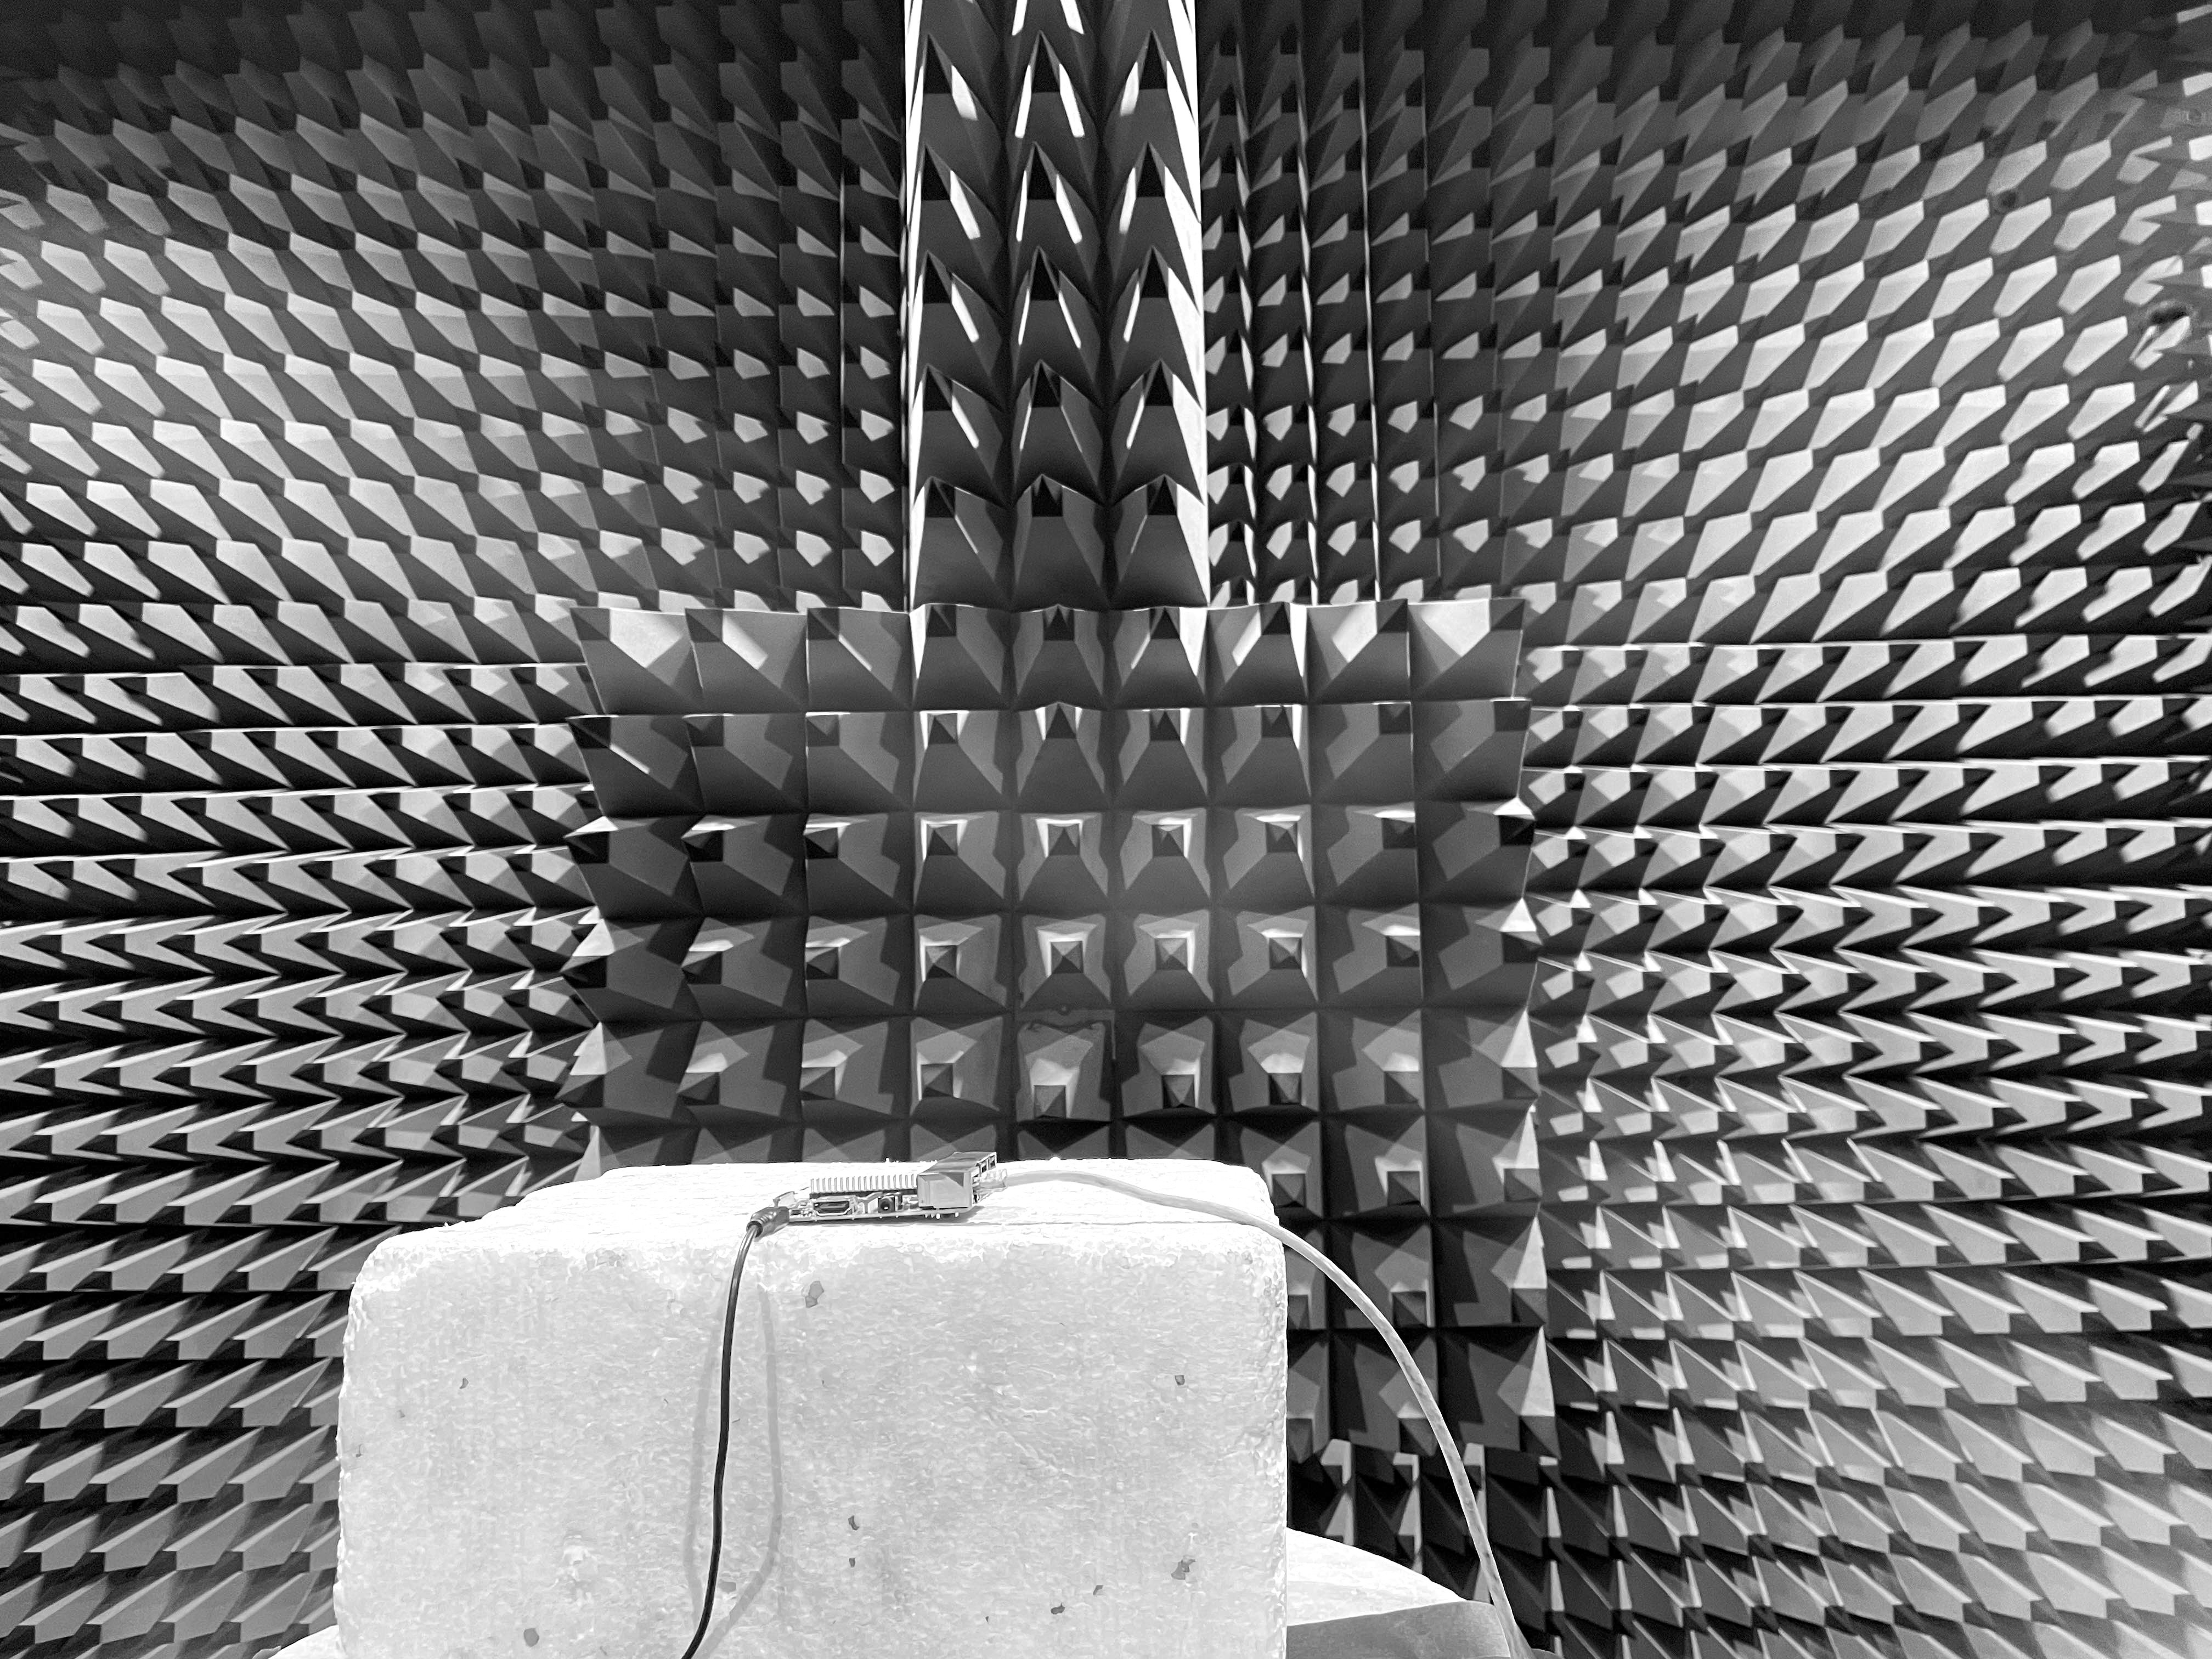
\includegraphics[width=0.8\textwidth]{fig/ch15/rasp_komora.jpg} % bez rozszerzenia
    \caption{Urządzenie Raspberry Pi 3 umieszczone w komorze kontroli szumu.}
    \label{fig:rasp_komora}
\end{figure}

\subsection{Konfiguracja urządzeń transmisyjnych}
Urządzenia transmisyjne to Raspberry Pi 3 z zainstalowanym na wymiennym nośniku pamięci systemem operacyjnym Raspberry Pi OS (Legacy, 32-bit). Dla każdego z pięciu urządzeń użyto tej samej karty micro-SD, co zagwarantowało urządzeniom te same ustawienia systemowe. Do skonfigurowania systemu jako punktu dostępu sieci wykorzystano otwarto-źródłowy sterownik \textit{hostapd}\footnote{~\url{https://manpages.debian.org/testing/hostapd/hostapd.8.en.html}}. Za kontrolę emisji wszystkich modułów radiowych (Wi-Fi, Bluetooth) odpowiadało również otwarto-źródłowe oprogramowanie \textit{rfkill}\footnote{~\url{https://linux.die.net/man/1/rfkill}}, którego użycie przedstawia listing ~\ref{listing:rfkill}.

Z ustawień przedstawionych na listingu ~\ref{listing:hostapd} szczególnie istotne dla przebiegu pomiarów były parametry, takie jak:
\begin{itemize}
    \item Nazwa sieci zdefiniowana jako "fingerprint".
    \item Częstotliwość nośna sygnału, zgodnie ze standardem \textit{channel=9}, definiuje środkową częstotliwość fali na 2452 MHz.
    \item Standard IEEE 802.11n zdefiniowany jako \textit{hw\_mode=n}.
    \item Okres rozgłaszania sygnału SSID jako \textit{beacon\_int=15}.
\end{itemize}
%\vspace{-4 mm}
\begin{listing}
\begin{minted}{shell}  
piotr@raspberrypi:~ $ cat /etc/hostapd/hostapd.conf
country_code=PL
interface=wlan0
ssid=fingerprint
channel=9
auth_algs=1
hw_mode=n
wpa=2
wpa_passphrase=korycki123
wpa_key_mgmt=WPA-PSK
wpa_pairwise=TKIP CCMP
rsn_pairwise=CCMP
beacon_int=15
\end{minted}
\caption{Plik konfiguracyjny routera hostapd} \label{listing:hostapd}
\end{listing}

\begin{listing}
\begin{minted}{shell}  
piotr@raspberrypi:~ $ rfkill list
0: phy0: Wireless LAN
        Soft blocked: no
        Hard blocked: no
1: hci0: Bluetooth
        Soft blocked: yes
        Hard blocked: no
\end{minted}
\caption{Odłączenie sygnału Bluetooth za pomocą rfkill} \label{listing:rfkill}
\end{listing}
%\vspace{-1 cm}
\subsection{Analizator widma Rohde \& Schwarz FSW-43}
Do zebrania sygnału referencyjnego, który informował o tym, czy sygnał jest nadawany prawidłowo, posłużyła aparatura pomiarowa, w którą była wyposażona komora EMC. Na rysunku ~\ref{fig:beacon_freq} została przedstawiona fala nośna o zdefiniowanej przez standard szerokości pasma 20 MHz, na której odbywa się transmisja sygnału SSID.
\begin{figure}[ht]
    \centering
    \includegraphics[width=0.7\textwidth]{fig/ch15/beacon.png} % bez rozszerzenia
    \caption{Zarejestrowany analizatorem widmowym sygnał w dziedzinie częstotliwości}
    \label{fig:beacon_freq}
\end{figure}
\subsection{Oscyloskop Tektronix MSO64B}
Dokładny przebieg amplitudy sygnału w czasie został zmierzony za pomocą oscyloskopu. Z uwagi na brak obsługi protokołu synchronizacji DSSS (Direct Sequence Spread Spectrum), w którym pracują urządzenia Wi-Fi 4, niemożliwym było zebranie prawidłowo zsynchronizowanego sygnału z częstotliwością próbkowania równą środkowej częstotliwości pasma. Przykład takiego błędu przedstawia wykres ~\ref{fig:sample_fault}.


\begin{figure}[ht]
    \centering
    \includegraphics[width=0.7\textwidth]{fig/ch15/sample_f_corr.png} % bez rozszerzenia
    \caption{Rozbieżność między transmitowanym oraz odbieranym sygnałem cyfrowym}
    \label{fig:sample_fault}
\end{figure}

W celu prawidłowej rekonstrukcji sygnału należy spełnić warunek twierdzenia Nyquista-Shannona, który mówi, że próbkowanie musi odbywać się z częstotliwością co najmniej dwukrotnie większą od szerokości pasma sygnału, a nie jego maksymalnej częstotliwości. Dla sygnału Wi-Fi o szerokości pasma $BW=20$ MHz wystarczy zatem częstotliwość próbkowania \( 40 \, \text{MHz} \), pod warunkiem sprowadzenia sygnału do pasma podstawowego. W praktyce parametry oscyloskopu pozwoliły na maksymalną częstotliwość próbkowania równą 25 GHz, co umożliwia poprawne próbkowanie sygnału o szerokości pasma 12,5 GHz. Oznacza to, że na każdy okres sygnału o częstotliwości 2462 MHz przypada od 9 do 10 próbek. Wysoka częstotliwość próbkowania umożliwia dokładną rejestrację sygnału oraz analizy zniekształceń, co demonstruje wykres ~\ref{fig:recon}.


\begin{figure}[ht]
    \centering
    \includegraphics[width=0.7\textwidth]{fig/ch15/rekonstrukcja.png} % bez rozszerzenia
    \caption{Rekonstrukcja sygnału dla stosunku próbkowania do transmisji 10:1}
    \label{fig:recon}
\end{figure}

Zgodnie z wyżej wymienionymi założeniami, na oscyloskopie zarejestrowano w formacie \textit{.mat} po 100 milionów próbek rzeczywistego sygnału Beacon dla wszystkich badanych płytek Raspberry Pi 3. Przykładowe prezentacje amplitudy w czasie dla płytki A zostały przedstawione na rysunkach ~\ref{fig:A_rela} i ~\ref{fig:A_rela50}. Należy jednak zwrócić uwagę na to, że zgodnie z wykresem ~\ref{fig:A_rela} oscyloskop jako sygnał referencyjny na początku oraz na końcu pomiaru zebrał również próbki szumu termicznego pomiędzy transmisjami, co można wywnioskować po tym, że zgodnie z konfiguracją routera ~\ref{listing:hostapd} oraz równaniem ~\ref{eq:timeVal}, okres przerwy między ramkami Beacon  wynosi 15,64 ms, a czas trwania całego zmierzonego sygnału to tylko 4 ms. Po odpowiednim przetworzeniu to właśnie te dane posłużyły do dalszej analizy opisanej w~pozostałej części pracy.

\begin{equation}
t = \frac{n}{f_s} = \frac{10^8}{2.5 \times 10^{10}} = 0.004 \, \text{s}
\label{eq:timeVal}
\end{equation}

\noindent gdzie:
\begin{itemize}
    \item $t$ - czas trwania sygnału,
    \item $f_s$ - częstotliwość próbkowania,
    \item $n$ - liczba próbek sygnału.
\end{itemize}


\begin{figure}[ht]
    \centering
    \includegraphics[width=0.7\textwidth]{fig/ch15/A_real.png} % bez rozszerzenia
    \caption{Zarejestrowany oscyloskopem sygnał dla płytki o etykiecie A (100 milionów próbek)}
    \label{fig:A_rela}
\end{figure}

\begin{figure}[ht]
    \centering
    \includegraphics[width=0.7\textwidth]{fig/ch15/A_real_50.png} % bez rozszerzenia
    \caption{Zarejestrowany oscyloskopem sygnał dla płytki o etykiecie A (50 tysięcy próbek)}
    \label{fig:A_rela50}
\end{figure}

\subsection{Wstępne przetwarzanie danych}
W celu dalszej analizy surowe dane pozyskane z oscyloskopu są przetwarzane aby usunąć z nagrania sygnału nadmiarowe dane oraz aby przetransformować sygnał rzeczywisty na reprezentację IQ.
\subsubsection{Format danych wejściowych}
Zgodnie z ustaleniami z poprzedniego rozdziału do dalszej części projektu posłużyły próbki sygnału oraz czasu zarejestrowane przez oscyloskop Tektronix MSO64B zapisane w formacie \textit{.mat}. Na przykładowym nagraniu sygnału w dziedzinie czasu przedstawionym na wykresie ~\ref{fig:A_rela} można zaobserwować, że duża część zebranych próbek to referencyjny szum termiczny, który na etapie analizy różnicy w transmisjach poszczególnych urządzeń Raspberry Pi 3 nie jest uwzględniany. Ponadto, analiza ma dotyczyć sygnału w~formacie IQ. Ponieważ wyniki pomiarów zostały zapisane w formacie \textit{.mat} który zawiera sygnał rzeczywisty dlatego konieczna jest transformacja do IQ w oparciu o dostępne metadane sygnału (częstotliwość środka pasma).
\subsubsection{Algorytmy wycinania szumu termicznego}
Celem algorytmów zaproponowanych w tej sekcji jest odseparowanie sygnału od stanowiących początek i koniec nagrania próbek szumu termicznego. Jak widać na wykresie ~\ref{fig:sig_begin}, w nagraniu sygnału również są zarejestrowane próbki o niskiej amplitudzie, w związku z czym niemożliwym było podzielenie próbek według kryterium wysokości amplitudy. W celu rozwiązania tego problemu pierwszym krokiem algorytmu jest podzielenie nagrania na równe odcinki o ustalonej długości i wyliczenie na ich podstawie lokalnych maksimów.

\begin{figure}[ht]
    \centering
    \includegraphics[width=0.8\textwidth]{fig/ch15/poczatek.png} % bez rozszerzenia
    \caption{Przejście szumu w sygnał.}
    \label{fig:sig_begin}
\end{figure}
\paragraph{\textit{Algorytm DecMax}}
Przedstawiony na listingu ~\ref{alg:dec_max} algorytm DecMax realizuje decymację sygnału na lokalne maksima przedziałów o zadanej długości, na podstawie których można analizować dane pod kątem trendu, a nie zawierających próbki szumu i sygnału pojedynczych wartości amplitudy. Ze względu na to, że sygnał oscyluje wokół ujemnych i dodatnich wartości napięcia, konieczne jest wyliczanie maksimów po wartości bezwzględnej amplitudy.
% \begin{algorithm}
% \caption{Decymacja sygnału z maksymalną wartością w przedziale}\label{alg:dec_max}
% \begin{algorithmic}[1]
% \Function{DecMax}{\textit{signal}, $n$}
%     \State \textit{m} $\gets \lfloor\frac{\textit{length(signal)} - n}{n}\rfloor + 1$\;
%     \State \textit{decimated} $\gets [1, \dots, m]$\;
%     \For{$i = 1$ \textbf{to} \textit{length(signal)} $- n$ \textbf{step} $n$}
%         \State \textit{window\_max} $\gets \max\left(\left| \textit{signal}[i : i+n] \right|\right)$\;
%         \State $\textit{decimated}[i] \gets \textit{window\_max}$\;
%     \EndFor
%     \State \Return \textit{decimated}
% \EndFunction
% \end{algorithmic}
% \end{algorithm}

\begin{algorithm}[H]
\DontPrintSemicolon
\LinesNumbered
\SetKwInOut{Input}{Input}
\SetKwInOut{Output}{Output}

\Input{signal, $n$}
\Output{decimated signal}

\BlankLine
$m \gets \lfloor (\text{length(signal)} - n)/n \rfloor + 1$\;
decimated $\gets$ array of length $m$\;

\For{$k \gets 0$ \textbf{to} $m-1$}{
    $i \gets k \cdot n + 1$\;
    window\_max $\gets \max(|\text{signal}[i : i+n]|)$\;
    decimated[$k+1$] $\gets$ window\_max\;
}

\Return decimated\;
\caption{Decymacja sygnału z maksymalną wartością w przedziale}
\label{alg:dec_max}
\end{algorithm}


Przykład sygnału po decymacji przedstawiony jest na wykresie ~\ref{fig:max}.
\begin{figure}[ht]
    \centering
    \includegraphics[width=0.7\textwidth]{fig/ch15/maksima.png} % bez rozszerzenia
    \caption{Przykład lokalnych maksimów sygnału dla przedziałów o~długości 10000 próbek.}
    \label{fig:max}
\end{figure}

\paragraph{\textit{Algorytm DegMax}}
Po otrzymaniu maksimów sygnału po decymacji możliwe jest ustalenie metody detekcji zmiany trendu. Jak można wywnioskować z wykresu ~\ref{fig:straights} punkty charakterystyczne dla początku (ale również końca) sygnału odznaczają się dużą różnicą amplitudy w stosunku do próbek szumu. Jeśli każde kolejne dwa punkty zostaną połączone odcinkiem prostym (kolor czerwony), można zauważyć, że kąt $\alpha$, jaki odcinek tworzy z prostą o równaniu $y=0$, odwzorowuje wspomniane wahania amplitudy i~jest możliwy do obliczenia zgodnie ze wzorem ~\ref{eq:degree}.

\begin{equation}
\alpha = \arctan(\tan(\alpha)) = \arctan(\frac{|a_1 - a_2|}{d}),
\label{eq:degree}
\end{equation}
gdzie
\begin{itemize}
    \item $a_1$, $a_2$-amplitudy dwóch kolejnych próbek
    \item $d$-ustalona odległość między próbkami, może wynosić 1
\end{itemize}

\begin{figure}[ht]
    \centering
    \includegraphics[width=0.75\textwidth]{fig/ch15/maks_przejscie.png} % bez rozszerzenia
    \caption{Przykład lokalnych maksimów sygnału dla przedziałów o~długości 10000 próbek z naniesionymi prostymi.}
    \label{fig:straights}
\end{figure}

Na bazie powyższych wniosków celem algorytmu jest obliczenie kątów między odcinkami łączącymi kolejne próbki, a prostą o równaniu $y=0$. Pseudokod algorytmu przedstawia listing ~\ref{alg:fill_deg}. Przykładowe wyniki algorytmów DecMax i~DegMax zostały umieszczone na wykresie ~\ref{fig:trim_logs}. Jak można zaobserwować na przecięciu sygnału oraz szumu, wartości kątów są największe, co stanowi kryterium cięcia.

% \begin{algorithm}
% \caption{Obliczanie kątów między sąsiednimi próbkami sygnału}\label{alg:fill_deg}
% \begin{algorithmic}[1]
% \Function{DegMax}{\textit{signal}, $d$}
%     \State \textit{n} $\gets \textit{length(signal)} - 2$
%     \State \textit{degrees} $\gets [1, \dots, n]$
%     \For{$i = 1$ \textbf{to} \textit{length(signal)} $- 2$}
%         \State \textit{diff} $\gets \left|\textit{signal}[i] - \textit{signal}[i+1]\right|$
%         \State \textit{angle} $\gets \arctan\left(\frac{\textit{diff}}{d}\right)$
%         \State $\textit{degrees}[i] \gets \textit{angle}$
%     \EndFor
%     \State \Return \textit{degrees}
% \EndFunction
% \end{algorithmic}
% \end{algorithm}

\begin{algorithm}[H]
\DontPrintSemicolon
\LinesNumbered
\SetKwInOut{Input}{Input}
\SetKwInOut{Output}{Output}
\Input{signal, $d$}
\Output{degrees between consecutive signal samples}
\BlankLine
$n \gets \text{length(signal)} - 2$\;
degrees $\gets$ array of length $n$\;
\For{$i \gets 1$ \KwTo length(signal) $- 2$}{
    diff $\gets |\text{signal}[i] - \text{signal}[i+1]|$\;
    angle $\gets \arctan(diff / d)$\;
    degrees[$i$] $\gets$ angle\;
}
\Return degrees\;
\caption{Obliczanie kątów między sąsiednimi próbkami sygnału}
\label{alg:fill_deg}
\end{algorithm}



\begin{figure}[ht]
    \centering
    \includegraphics[width=0.8\textwidth]{fig/ch15/probka_E_25GS_logs.png} % bez rozszerzenia
    \caption{Wykresy lokalnych maksimów oraz kątów nachylenia prostych dla sygnału płytki E i długości przedziałów równej 10000.}
    \label{fig:trim_logs}
\end{figure}

\paragraph{\textit{Algorytm TriMax}}
Algorytm przycinania sygnału (TriMax) działa z wykorzystaniem informacji dostarczonych przez powyższe rozwiązania. TriMax korzysta również z funkcji $twomax(wektor)$, która stanowi prostą modyfikację algorytmu wyszukiwania elementu maksymalnego, zwracającą indeksy dwóch największych elementów w wektorze w czasie liniowym. Metoda ta polega na wyznaczeniu krańców sygnału na podstawie dwóch maksymalnych wartości kątów i przycięciu danych o amplitudzie i czasie w tak wyznaczonych granicach. Listing ~\ref{listing:trimax} przedstawia zastosowaną w projekcie implementację algorytmu w języku Julia. Złożoność algorytmu $T(n)$, liczona jako suma złożoności wywołanych pojedynczo funkcji, wynosi $O(n)$, ponieważ każda z nich ma złożoność również $O(n)$.
\begin{listing}[H]
\begin{minted}{julia}
function TriMax(signal, time; n=10000)
    decimated_max = DecMax(signal, n=n)
    degrees = DegMax(decimated_max)
    i, j = TwoMax(angles)
    i *= n
    j *= n
    if (i < j)
        return signal[i:j], time[i:j]
    else
        return signal[j:i], time[j:i]
    end
end
\end{minted}
\caption{Implementacja algorytmu TriMax w języku Julia.} \label{listing:trimax}
\end{listing}

% \subsubsection{Demodulacja sygnału}
% W celu doprowadzenia sygnału do formy, w jakiej nadajnik prowadził transmisję, należało dodatkowo zdemodulować dane w oparciu o schemat modulacji QAM. Schemat modulacji przedstawiony na diagramie ~\ref{fig:qam_mod} demonstruje, że wyemitowana fala to w rzeczywistości suma dwóch sygnałów przesuniętych w fazie o $90^{\circ}$. W celu odwrócenia procesu modulacji wystarczyło więc przemnożyć zarejestrowany sygnał przez fale o częstotliwości $f_c=2452$ MHz określone równaniami ~\ref{eq:I_carrier} oraz ~\ref{eq:Q_carrier}. Listing ~\ref{listing:demod} przedstawia zastosowaną w programie implementację demodulacji kwadraturowo-amplitudowej.
% \begin{equation}
% I_{carrier}= \cos(2\pi f_c t) \label{eq:I_carrier}
% \end{equation}
% \begin{equation}
% Q_{carrier} = \sin(2\pi f_c t) \label{eq:Q_carrier}
% \end{equation}


% %Listing ~\ref{listing:demod} przedstawia zastosowaną w programie implementację demodulacji kwadraturowo-amplitudowej.

% \begin{figure}[ht]
%     \centering
%     \includegraphics[width=0.8\textwidth]{fig/ch15/generation-of-QAM-signal.png} % bez rozszerzenia
%     \caption{Schemat modulacji QAM na podstawie \cite{qam_website}.}
%     \label{fig:qam_mod}
% \end{figure}

% \begin{listing}
% \begin{minted}{julia}
% function demodulate(signal, t; carrier_freq=2.452e9)
%     I_carrier = cos.(2 * pi * carrier_freq .* t)
%     Q_carrier = sin.(2 * pi * carrier_freq .* t)
%     return signal .* I_carrier, signal .* Q_carrier
% end
% \end{minted}
% \caption{Implementacja demodulacji QAM w języku Julia.} \label{listing:demod}
% \end{listing}
\subsubsection{Aplikacja Trimmer}
Program służący do wstępnej obróbki danych pomiarowych przed etapem dalszej analizy został napisany z wykorzystaniem powyższych algorytmów. Aplikacja została zaimplementowana w języku Julia ze względu oraz obsługę plików w~formacie \textit{.mat}. Przy wywołaniu z linii komend program przyjmuje następujące argumenty:
\begin{itemize}
    \item \texttt{---upscale} włącza konwersję jednostki amplitudy na mV.
    \item \texttt{---raw} pozwala na zapisanie przyciętego sygnału w postaci rzeczywistej bez transformacji na format IQ.
    % \item Flaga \texttt{---iq} pozwalająca na zapisanie przyciętego sygnału w postaci zdemodulowanej.
    \item \texttt{---input} po którym należy wpisać ścieżkę pliku wejściowego w formacie \textit{.mat}.
    \item \texttt{---frequency} określająca częstotliwość fali nośnej w MHz potrzebną do demodulacji sygnału.
    \item \texttt{---verbose} umożliwia zapisanie wykresów parametrów, a także odcinków początku i końca sygnału dla zwiększenia ilości informacji o~procesie przetwarzania danych.
    \item \texttt{title} pozwala określić tytuł wykresów generowanych w trybie \texttt{verbose}.
\end{itemize}
Po zakończeniu działania program Trimmer zapisuje przycięte dane ponownie w formacie \textit{.mat}. Efekty działania aplikacji zostały zaprezentowane na wykresie ~\ref{fig:trim_begin}.%, ~\ref{fig:trim_demod} i ~\ref{fig:trim_const}.
\begin{figure}[ht]
    \centering
    \includegraphics[width=0.8\textwidth]{fig/ch15/probka_E_25GS_begin.png} % bez rozszerzenia
    \caption{Wykres początku przyciętego sygnału dla płytki E.}
    \label{fig:trim_begin}
\end{figure}

% \begin{figure}[ht]
%     \centering
%     \includegraphics[width=0.8\textwidth]{fig/ch15/timedomainiq.png} % bez rozszerzenia
%     \caption{Wykres zdemodulowanego sygnału dla płytki E.}
%     \label{fig:trim_demod}
% \end{figure}

% \begin{figure}[ht]
%     \centering
%     \includegraphics[width=0.8\textwidth]{fig/ch15/constellationiq.png} % bez rozszerzenia
%     \caption{Wykres konstelacji sygnału po demodulacji dla płytki E.}
%     \label{fig:trim_const}
% \end{figure}


\section{Analiza i klasyfikacja danych}
W tej sekcji przedstawione są metody analizy wstępnie przetworzonych próbek. Celem analizy jest zbadanie możliwości klasyfikacji urządzeń dzięki unikalnym niedoskonałościom urządzeń transmisyjnych, a w szczególności niedoskonałościach balansu amplitudy.
% \subsection{Przesunięcie sygnału w fazie}
% W celu zbadania przebiegu fazy sygnału w czasie oraz ewentualnych różnic w otrzymanych wynikach pomiędzy testowanymi urządzeniami należało zaimplementować algorytm zliczający narastające opóźnienie fazy. Wejściem programu były zdemodulowane dane otrzymane za pomocą algorytmu TriMax, a efektem pracy algorytmu były dane przedstawiające zmianę fazy na przestrzeni zarejestrowanego sygnału.
% \paragraph{Analiza centroidów}
% Z uwagi na to, że posługujemy się rekonstrukcją, a nie zsynchronizowanymi próbkami wyemitowanego sygnału, koniecznym było wyznaczenie takiej wielkości próbki danych, jaka będzie reprezentatywna dla wszystkich rejestrowanych wartości centroidu. Jak widać na wykresach ~\ref{fig:iq10k}, przykładowy przedział zawierający 10 000 symboli IQ jest niewystarczający, więc w dalszej części badań pojedyncza próbka konstelacji miała długość 100 000 symboli.

% \begin{figure}[ht] 
% 	\centering
% 	\begin{minipage}[b]{0.45\textwidth}
% 		\centering\includegraphics[width=0.9\textwidth]{fig/ch15/c10k.png} % left figure
% 	\end{minipage}
% 	\begin{minipage}[b]{0.45\textwidth}
% 		\centering
% 		\includegraphics[width=0.9\textwidth]{fig/ch15/c100k.png} % right figure
% 	\end{minipage}
%     \caption{Porównanie wykresów konstelacji zdemodulowanego sygnału dla płytki E}\label{fig:iq10k}
% \end{figure}

% Jeśli nałożymy na siebie wykresy dwóch kolejnych odcinków (wykres ~\ref{fig:c200k}), możemy zaobserwować wyraźny obrót następujących po sobie centroidów wokół punktu $(0,0)$. Jest to nic innego jak rotacja liczb zespolonych składających się na przedstawione centroidy o dany kąt $\phi$ równy skumulowanemu przesunięciu w fazie sygnału. Dzięki analizie rotacji centroidów możliwe było oszacowanie charakterystyki badanego nadajnika, do czego posłużył Algorytm Detekcji Oszacowanej Fazy.
% \begin{figure}[ht]
%     \centering
%     \includegraphics[width=0.8\textwidth]{fig/ch15/c200k.png} % bez rozszerzenia
%     \caption{Wykres konstelacji dwóch odcinków zdemodulowanego sygnału dla płytki E.}
%     \label{fig:c200k}
% \end{figure}

% \subsubsection{Algorytm detekcji oszacowanej fazy}
% ADOF, przedstawiony w pseudokodzie ~\ref{alg:ADOF}, dzieląc sygnał na odcinki długości $k$, w pierwszym kroku klasyfikuje centroidy za pomocą algorytmu k-średnich. Ze względu na wysoką precyzję wykonanych pomiarów oraz fakt, że zebrane próbki zawierają również szum termiczny, na każdym wykresie konstelacji nastąpiła duża koncentracja danych wokół punktu $(0,0)$, co doprowadziło do sytuacji, w której kMeans nie mógł poprawnie sklasyfikować dwóch centroidów. Przykład pochłaniania jednego centroidu przez drugi wokół obszaru niskich amplitud przedstawia wykres ~\ref{fig:pochlanianie}. W celu uniknięcia błędnej klasyfikacji, do wejścia algorytmu k-średnich dodany został trzeci centroid niskich amplitud rozpoznawany po tym, że jego odległość w metryce euklidesowej od punktu $(0,0)$ jest najmniejsza. Centroidy $\alpha$ i $\beta$ są przypisywane w dowolnej kolejności.

% W dalszej części algorytm, iterując po kolejnych przedziałach długości $k$, ponownie wylicza środki centroidów, a następnie klasyfikuje je w oparciu o odległość euklidesową od środka centroidu poprzedniego przedziału. Faza tak sklasyfikowanych punktów obliczana jest ze współrzędnych poprzez rozszerzenie funkcji $\arctan()$, która dla uniknięcia wartości ujemnych zwraca kąt z przedziału $[0, 2\pi]$. Każde wywołanie funkcji $\textit{collectCenters(centroids\_map, center\_alpha, center\_beta, mid\_point, c)}$ uzupełnia wektory przypisane w strukturze \textit{centroids\_map} do centroidów $\alpha$, $\beta$ i \textit{S} o podane punkty na pozycji \textit{c}.


% Implementację struktury centroids\_map w języku Python, która służy do przechowywania danych o współrzędnych i fazie środków centroidów, przedstawia listing ~\ref{listing:map}.

% \begin{listing}
% \begin{minted}{python}
% import numpy as np
% iter = n//k
% one_centroid_map = {
%         "I": np.zeros(iter),
%         "Q": np.zeros(iter),
%         "phase": np.zeros(iter)
%     }
% centroids_map = {
%     "A": one_centroid_map,
%     "S": one_centroid_map,
%     "B": one_centroid_map
% }
% \end{minted}
% \caption{Implementacja struktury danych odpowiadającej za przechowywanie informacji o centroidach.} \label{listing:map}
% \end{listing}


% \begin{figure}[ht] 
% 	\centering
% 	\begin{minipage}[b]{0.45\textwidth}
% 		\centering\includegraphics[width=1\textwidth]{fig/ch15/clusters22_E.png} % left figure
% 	\end{minipage}
% 	\begin{minipage}[b]{0.45\textwidth}
% 		\centering
% 		\includegraphics[width=1\textwidth]{fig/ch15/clusters2_E.png} % right figure
% 	\end{minipage}
%     \caption{Porównanie klasyfikacji centroidów zdemodulowanego sygnału dla płytki E}\label{fig:pochlanianie}
% \end{figure}

% \begin{algorithm}
% \caption{Algorytm ADOF do analizy sygnałów I i Q}\label{alg:ADOF}
% \begin{algorithmic}[1]
% \Function{ADOF}{\textit{I}, \textit{Q}, $n$, $k \gets 100000$}
%     \State $c \gets 1$
%     %\State \textit{iter} $\gets \lfloor \frac{n}{k} \rfloor$
%     \State \textit{centroids\_map} $\gets$ pusty słownik
%     \State \textit{centers} $\gets$ \textit{kMeans}(\textit{I}[1:$k$], \textit{Q}[1:$k$], 3)
%     \State \textit{distances} $\gets$ \textit{Euclidean}((0, 0), \textit{centers})
%     \State $i_{\text{mid}} \gets \textit{argMin}(\textit{distances})$
%     \State \textit{mid\_point} $\gets$ \textit{centers}[$i_{\text{mid}}$]
%     \State \textit{erase}(\textit{centers}, \textit{mid\_point})
%     \State \textit{collectCenters}(\textit{centroids\_map}, \textit{centers}[1], \textit{centers}[2], \textit{mid\_point}, \textit{c})
%     \State $c \gets c + 1$

%     \For{$i = k$ \textbf{to} $n - k$ \textbf{step} $k$}
%         \State \textit{centers} $\gets$ \textit{kMeans}(\textit{I}[$i:i+k$], \textit{Q}[$i:i+k$], 3)
%         \State \textit{distances} $\gets$ \textit{Euclidean}((0, 0), \textit{centers})
%         \State $i_{\text{mid}} \gets \textit{argMin}(\textit{distances})$
%         \State \textit{mid\_point} $\gets$ \textit{centers}[$i_{\text{mid}}$]
%         \State \textit{erase}(\textit{centers}, \textit{mid\_point})
%         \State \textit{distances\_alpha} $\gets$ \textit{Euclidean}(\textit{getAlpha}(\textit{centroid\_map}), \textit{centers})
%         \State \textit{distances\_beta} $\gets$ \textit{Euclidean}(\textit{getBeta}(\textit{centroid\_map}), \textit{centers})
%         \State \textit{center\_alpha} $\gets$ \textit{centers}[\textit{argMin}(\textit{distances\_alpha})]
%         \State \textit{center\_beta} $\gets$ \textit{centers}[\textit{argMin}(\textit{distances\_beta})]
%         \State \textit{collectCenters}(\textit{centroids\_map}, \textit{center\_alpha}, \textit{center\_beta, \textit{mid\_point}, \textit{c}})
%         \State $c \gets c + 1$
%     \EndFor
%     \State \Return \textit{centroids\_map}
% \EndFunction
% \end{algorithmic}
% \end{algorithm}

% \subsubsection{Analiza złożności algorytmu ADOF}
% Algorytm wykonując pętlę o długości $\lfloor \frac{n}{k} \rfloor$ w każdym kroku:
% \begin{enumerate}
%     \item Wywołuje algorytm k-średnich dla:
%     \begin{itemize}
%         \item Dwóch wymiarów danych $d$.
%         \item Trzech klastrów $a$.
%         \item Domyślnej liczby iteracji konwergencji $i=20$.
%         \item Rozmiaru wektorów $I$ i $Q$ równego k.
%     \end{itemize}
%     \item W stałym czasie klasyfikuje środki centroidów.
%     \item W stałym czasie uzupełnia strukturę centroid\_map o wyliczone dane.
% \end{enumerate}
% Zgodnie ze specyfikacją algorytmu k-średnich w bibliotece SciPy \cite{scipy_kmeans_reference}, funkcja ta jest określona złożonością $O(a\cdot d\cdot i \cdot k)$, stąd ADOF ma złożoność $\theta(\lfloor \frac{n}{k} \rfloor)\cdot O(a\cdot d\cdot i \cdot k) = O(\lfloor \frac{n}{k} \rfloor)\cdot O(3\cdot 2\cdot i \cdot k) = O(n\cdot i)$.

% \subsubsection{Interpretacja wyników}
% Algorytm poprawnie zarejestrował przebieg fazy sygnału dla wszystkich badanych płytek. Wykresy ~\ref{fig:mids} przedstawiają położenie wszystkich zarejestrowanych środków ciężkości. Dla lepszej prezentacji wyniku współrzędne centroidu $\alpha$ zostały przesunięte o wektor $(5,5)$.

% Na wykresie ~\ref{fig:phase} została przedstawiona zakumulowana faza sygnału w czasie. Wykres ~\ref{fig:vectors} ilustruje fragment rotacji centroidu.

% \begin{figure}[ht] 
% 	\centering
% 	\begin{minipage}[b]{0.45\textwidth}
% 		\centering\includegraphics[width=1\textwidth]{fig/ch15/centers_shifted_D.png} % left figure
% 	\end{minipage}
% 	\begin{minipage}[b]{0.45\textwidth}
% 		\centering
% 		\includegraphics[width=1\textwidth]{fig/ch15/centers_shifted_E.png} % right figure
% 	\end{minipage}
%     \caption{Przebieg położenia środków centroidów.}\label{fig:mids}
% \end{figure}

% \begin{figure}[ht] 
% 	\centering
% 	\begin{minipage}[b]{0.45\textwidth}
% 		\centering\includegraphics[width=1\textwidth]{fig/ch15/phase_sum_D.png} % left figure
% 	\end{minipage}
% 	\begin{minipage}[b]{0.45\textwidth}
% 		\centering
% 		\includegraphics[width=1\textwidth]{fig/ch15/phase_sum_E.png} % right figure
% 	\end{minipage}
%     \caption{Suma krocząca fazy centroidów}\label{fig:phase}
% \end{figure}

% \begin{figure}[ht]
%     \centering
%     \includegraphics[width=0.8\textwidth]{fig/ch15/centers_shifted_arrow_E.png} % bez rozszerzenia
%     \caption{Wykres przebiegu położenia środka centroidu z naniesionym kierunkiem rotacji dla płytki E.}
%     \label{fig:vectors}
% \end{figure}
% Wyniki działania algorytmu dla wszystkich urządzeń z fazą mierzoną w radianach zostały zaprezentowane w tabeli ~\ref{table:phase}.
%     \begin{table}[ht]
% \centering
% \caption{Wyniki analizy przebiegu fazy liczonej w radianach.}
% \label{table:phase}
% \begin{tabular}{|c|c|c|c|}
% \hline

% 			\textbf{Płytka} & \textbf{Faza centroidu $\alpha$} & \textbf{Faza centroidu $\beta$} & \textbf{Liczba przedziałów}\\
% \hline
% 			A & 1230.11 & 1221.71 & 398 \\
%             \hline
% 			B & 1311.69 & 1301.20 & 398 \\
%             \hline
% 			C & 1161.54 & 1086.44 & 398 \\
%             \hline
%             D & 1224.98 & 1216.63 & 398 \\
%             \hline
%             E & 1269.37 & 1261.05 & 398 \\
%             \hline

% 		\end{tabular}

        
% 	\end{table}

\subsection{Niedoskonałości w amplitudzie}
W tej części opisane jest przystosowanie modelu neuronowej sieci konwolucyjnej, której głównym zadaniem jest rozpoznawanie fotografii, do klasyfikacji sygnału urządzeń po niedoskonałościach w wartości amplitudy. Motywacją do zastosowania tego modelu są obiecujące wyniki klasyfikacji sygnału opisane w pracy \cite{sankhe2019oracle}. W~tradycyjnym zastosowaniu modele neuronowych sieci konwolucyjnych jako dane wejściowe przyjmują wektorowe reprezentacje fotografii jako 3 kanały odpowiadające za wartości pikseli w domenie koloru (w reprezentacji r,g,b). 
% Pomysłem na modyfikację takiego modelu było wprowadzenie reprezentacji wektorowej jednego diagramu konstelacji IQ jako dwa kanały I i Q o długości 100000 próbek. Do implementacji modelu zastosowano bibliotekę PyTorch \cite{pytorch}.
\subsubsection{Klasa IQDataset}
IQDataset, przedstawiony na Listingu ~\ref{listing:dataset}, to klasa dziedzicząca po interfejsie Dataset w bibliotece PyTorch. Danymi wejściowymi klasy jest słownik porządkujący pary wektorów I i Q według etykiet urządzeń $\{A, B, C, D, E\}$. Nadpisana metoda \textit{\_\_get\_\_item()} odpowiada za konwersję sygnału do tensora, a także przepisanie etykiet urządzeń na akceptowane przez sieć neuronową liczby $\{0,1,2,3,4\}$.
\begin{listing}[H]
\begin{minted}[breaklines, breakanywhere]{python}
import torch
from torch.utils.data import Dataset, DataLoader
class IQDataset(Dataset):
    def __init__(self, training_data):
        total_samples = sum(len(data['I']) for data in training_data.values())
        self.samples = [None] * total_samples
        current_idx = 0
        for device, data in training_data.items():
            I_data = data['I']
            Q_data = data['Q']
            for i in range(len(I_data)):
                self.samples[current_idx] = {
                    'device': device,
                    'I': I_data[i],
                    'Q': Q_data[i],
                }
                current_idx += 1
    def __len__(self):
        return len(self.samples)
    def __getitem__(self, idx):
        sample = self.samples[idx]
        return {
            'input': torch.tensor([sample['I'], sample['Q']], dtype=torch.float32),
            'label': torch.tensor(label_to_tens(sample['device'])),
        }
\end{minted}
\caption{Implementacja klasy IQDataset w języku Python.} \label{listing:dataset}
\end{listing}
\subsubsection{Model sieci neuronowej}
W projekcie użyto sieci IQCNN, podobnej do modelu klasyfikacji sygnału przedstawionego w pracy \cite{sankhe2019oracle}. Sieć została zaprojektowana z myślą o odwzorowaniu procesu uczenia głębokiego dla obrazów na przetwarzanie diagramów konstelacji sygnału. Model można podzielić na następujące warstwy:
\begin{enumerate}
    \item Warstwa wejściowa o rozmiarze $1\times N \times 2$, gdzie $N=100000$.
    \item Pierwsza warstwa konwolucyjna odpowiadająca za ekstrakcję lokalnych cech i implementację filtrów. Warstwa ta posiada 16 filtrów, każdy o rozmiarze 5. Wejście warstwy ma rozmiary $(batch\_size, 2, 100000)$, a wyjście $(batch\_size, 16, 100000)$.
    \item Pierwsza warstwa Max Pooling odpowiadająca za redukcję wymiarowości danych. Wyjściowa wielkość danych to $(batch\_size, 16, 50000)$.
    \item Druga warstwa konwolucyjna odpowiadająca za dalsze wyszukiwanie cech posiada 32 filtry, również o rozmiarze 5. Finalnie całkoiwty rozmiar wyjścia wynosi $(batch\_size, 32, 50000)$.
    \item Druga warstwa Max Pooling odpowiadająca za spłaszczenie danych przed dalszym przetwarzaniem. Rozmiar wyjścia to $(batch\_size, 32, 25000)$.
    \item Warstwa spłaszczająca Flatten odpowiadająca za spłaszczenie danych przed dalszym przetwarzaniem. Wyjściowe wymiary tensora to $(batch\_size, 32\cdot 25000)$.
    \item Pierwsza warstwa w pełni połączona Fully Connected odpowiadająca za połączenie wejściowych neuronów do tensora o wymiarach $(batch\_size,128)$.
    \item Druga warstwa w pełni połączona odpowiadająca za końcową klasyfikację danych.
\end{enumerate}
Poglądowy schemat architektury sieci został opracowany w środowisku AlexNet\footnote{~\url{https://alexlenail.me/NN-SVG/AlexNet.html}} i jest przedstawiony na diagramie ~\ref{fig:alexnet}.
\begin{figure}[ht]
    \centering
    \includegraphics[width=0.7\textwidth]{fig/ch15/cnn_subtitled.png} % bez rozszerzenia
    \caption{Schemat architektury modelu IQCNN z oznaczeniami warstw oraz rozmiarami filtrów.}
    \label{fig:alexnet}
\end{figure}

% Proces trenowania modelu składa się z dziesięciu iteracji, w których zastosowano parametr liczby próbek przetwarzanych równolegle $batch\_size=64$. Obliczenia zotsały przeprowadzone na procesorze Intel Core i7-1270P 2.20 GHz dla $5\times39\times10^{9}$ próbek IQ trwały 27 minut, a końcowa dokładność treningu wyniosła 96,97\%. W trakcie tego procesu IQCNN wykształcił w sobie łączny zestaw cech rozmiaru 102403541 parametrów.

Do ewaluacji modelu użytych zostało $5\times8\times10^{5}$ próbek IQ, będących zbiorem rozłącznym od sygnału użytego w trakcie uczenia sieci, choć zarejestrowanym w~tych samych warunkach otoczenia. W trakcie ewaluacji przeprowadzone zostało łącznie 40 testów dla wszystkich urządzeń transmisyjnych, w których model poprawnie poprawnie klasyfikował etykietę urządzenia 36 razy, co daje końcową dokładność 90\%.

\section{Wnioski i podsumowanie}

W pracy zaproponowano metodę akwizycji sygnałów WiFi poprzez przeprowadzenie pomiarów na oscyloskopie Tektronix MSO64B. Zaimplementowano autorskie oprogramowanie mające na celu obróbkę surowych danych z oscyloskopu i klasyfikację sygnału testowanych urządzeń. Spełnia to najważniejsze założenie projektu oraz tworzy podstawy dla dalszego rozwoju technologii identyfikacji urządzeń nadawczych przy użyciu uczenia maszynowego. Przedstawione w pracy algorytmy wstępnego przetwarzania sygnału radiowego w czasie liniowym oraz modele klasyfikacji urządzeń po niedoskonałościach w emitowanym sygnale wykazały bardzo obiecujące wyniki,  90\% skutecznych identyfikacji w warunkach testowych, co uzasadnia kontynuację prac.
%
Proponowane dalsze kierunki badań i~rozwoju projektu to:
\begin{enumerate}   
 %   \item Oprogramowanie na układzie FPGA radia RFSoC 4x2 protokołu synchronizacji sygnału OFDM w celu odejścia od rekonstrukcji sygnału cyfrowego i zwiększenia wydajności przeprowadzanych pomiarów. Taka funkcjonalność umożliwiłaby także rejestrację sygnału w moulacjach wyższego rzędu, a także przeprowadzanie pomiarów na znacznie większym wachlarzu urządzeń, w tym m.in. na telefonach komórkowych.
    \item Zwiększenie liczby badanych urządzeń w celu dalszego rozwoju i testowania modelu IQCNN.
    \item Modyfikacja architektury sieci IQCNN w celu uwzględnienia i identyfikacji urządzeń nieuwzględnionych podczas trenowania sieci.
    \item Testowanie sieci IQCNN w rzeczywistych warunkach propagacyjnych z~uwzględnieniem kanału komunikacyjnego.
    \item Użycie dedykowanej i mobilnej platformy do akwizycji i lokalnego przetwarzania sygnałów, np. platformy RFSoC 4x2 firmy RealDigital,  oraz stworzenie infrastruktury odbiorczej dla łącza o wysokiej przepustowości w celu zmniejszenia kosztów prowadzenia badań.
\end{enumerate}

\begin{thebibliography}{20}

\bibitem{rf_fingerprinting_sciencedirect}
  Jagannath, A., Jagannath, J., and Kumar, P. S. P. V.: RF Fingerprinting: New Trends and Challenges, Computer Networks, 208, 2022, \doi{10.1016/j.comnet.2022.109455}
\bibitem{kaur2020rf}
Kaur, Su., Gupta, S. K., and Bedi, A. S.: RF fingerprinting and its challenges: A review, J. of Communications and Information Networks, 5, 2, pp.110--121, 2020, Springer,
  \doi{10.23919/JCIN.2020.9138953},
  \url{https://www.proquest.com/openview/cfeba7fedf593c467f91e7fa6b20e844/1}
  
\bibitem{sankhe2019oracle}
Sankhe, K. et al.: No Radio Left Behind: Radio Fingerprinting Through Deep Learning of Physical-Layer Hardware Impairments, IEEE Trans. on Cognitive Communications and Networking, 6, 1, pp.165-178, 2020, \doi{10.1109/TCCN.2019.2949308}

\bibitem{soltani2021RF}
Soltani, N. et al.: RF Fingerprinting Unmanned Aerial Vehicles With Non-Standard Transmitter Waveforms, IEEE Transactions on Vehicular Technology, 69, 12, pp.15518-15531, 2020, \doi{10.1109/TVT.2020.3042128}

\bibitem{8362982}
Zheng, J., and Lv, Y.: Likelihood-Based Automatic Modulation Classification in OFDM With Index Modulation, IEEE Trans. on Vehicular Technology, 67, 9, pp.8192-8204, 2018, \doi{10.1109/TVT.2018.2839735}

\bibitem{wang2016distributed}
Wang, B. et al.: Distributed Asynchronous Modulation Classification Based on Hybrid Maximum Likelihood Approach, IEEE Trans. on Wireless Communications, 15, 1, pp.411--422, 2016, \doi{10.1109/TWC.2015.2477051}, \url{https://www.researchgate.net/publication/288994862_Distributed_Asynchronous_Modulation_Classification_Based_on_Hybrid_Maximum_Likelihood_Approach/citations}

\bibitem{yang2024mitigatingreceiverimpactradio}
Yang, L. et al.: Mitigating Receiver Impact on Radio Frequency Fingerprint Identification via Domain Adaptation, IEEE Internet of Things Journal, 11, 13, pp.24024-24034, 2024, \doi{10.1109/JIOT.2024.3389491}
  
\bibitem{O_Shea_2018}
O’Shea, T. J., Roy, T., and Clancy, T. C.: Over-the-Air Deep Learning Based Radio Signal Classification, IEEE J. of Selected Topics in Signal Processing, 12, 1, pp.168–179, 2018, \url{http://dx.doi.org/10.1109/JSTSP.2018.2797022}, \doi{10.1109/jstsp.2018.2797022},


\bibitem{darpa_spectrum_2017}
DARPA : Engineering the Spectrum: Pioneering New Frontiers in Communications, 2017, Available at: \url{https://www.darpa.mil/news-events/2017-08-11a}, Accessed: 2024-12-11

\bibitem{NIPS2012_c399862d}
Krizhevsky, A., Sutskever, I., and Hinton, G. E.: ImageNet Classification with Deep Convolutional Neural Networks, In \textit{Advances in Neural Information Processing Systems}, Eds. F. Pereira et al., Curran Associates, Inc., 25, 2012, \url{https://proceedings.neurips.cc/paper_files/paper/2012/file/c399862d3b9d6b76c8436e924a68c45b-Paper.pdf}

\bibitem{he2015deepresiduallearningimage}
He, K. et al.: Deep Residual Learning for Image Recognition, resented at the Conference on Computer Vision and Pattern Recognition (CVPR), arXiv, 2015, \url{https://arxiv.org/abs/1512.03385}

\bibitem{10.1145/1409944.1409959}
Brik, V. et al.: Wireless device identification with radiometric signatures, Proc. of the 14th ACM Int. Conf. on Mobile Computing and Networking, ACM, 2008, pp. 116–127, \url{https://doi.org/10.1145/1409944.1409959}, \doi{10.1145/1409944.1409959},


\bibitem{9363693}
IEEE,: IEEE Standard for Information Technology--Telecommunications and Information Exchange between Systems - Local and Metropolitan Area Networks--Specific Requirements - Part 11: Wireless LAN Medium Access Control (MAC) and Physical Layer (PHY) Specifications, IEEE Std 802.11-2020 (Rev. of IEEE Std 802.11-2016), 2021, \doi={10.1109/IEEESTD.2021.9363693}

\end{thebibliography}
\newcommand{\p}{\mathcal{P}}
\chapterauthor{Joanna Balbus}
\chapter[Trwałość w układach \ldots]{Trwało\'s\'c w układach równa\'n reakcji -- dyfuzji z adwekcj\k{a}}
% \label{rffp} % Always give a unique label
% use \chaptermark{}
% to alter or adjust the chapter heading in the running head

\thispagestyle{empty}
\vspace{-8mm} {\large Joanna Balbus} \vspace{8mm}

	\section{Wprowadzenie}
	W ostatnich kilku latach wiele uwagi poświęca się modelom populacji w~środowisku jednorodnym lub niejednorodnym.
	Jednostajna trwałość, koegzystencja oraz wymieranie opisują istotne szczególne typy asymptotycznego zachowania rozwiązań powiązanych modeli. W niniejszej pracy badamy zagadnienie reakcji–dyfuzji typu Kołmogorowa z adwekcją
	
	\begin{equation}
		\label{1.1}
		% \tag{1.1}
		\begin{cases}
			u_{it}=\mu_i  u_{ixx}  -\alpha_i  u_{ix} + f_i(t,x,u_1,u_2)u_i, \quad t>0 \quad x\in (0,L),\quad i=1,2,\\
			u_i(0,x)=u_{i0}(x), \quad x\in (0,L),\quad i=1,2.
		\end{cases}
	\end{equation}
	z warunkami brzegowymi bez przepływu
	\begin{equation}
		\label{1.2}
		% \tag{1.2}
		\begin{cases}
			\mu_i u_{ix}(0,t) - \alpha_i u_i(0,t)=0, \quad t>0, \quad i=1,2, \\
			\mu_i u_{ix}(L,t) - \alpha_i u_i(L,t) = 0, \quad t>0, \quad i=1,2.
		\end{cases}
	\end{equation}
	
	W  literaturze istnieje wiele prac poświęconych równaniom reakcji–dyfuzji z adwekcją, zob. \cite{Hess,Huisman}, 
	\cite{Kolokolnikov,Lutscher},  \cite{Ma,Vasilyeva}, .
	Takie równania mogą być rozpatrywane z różnymi warunkami brzegowymi. W zależności od warunków brzegowych
	otrzymujemy odmienne scenariusze ekologiczne.
	
	Najbardziej ogólna postać warunków brzegowych to
	\begin{equation}
		\begin{cases}
			\mu_i u_{ix} - \alpha_i u_{i} =\tilde{b}_{i}\alpha_i u_i, \quad x=0,\quad i=1,2,\\
			\mu_i u_{ix} - \alpha_i u_{i} =-\hat{b}_{i}\alpha_i u_i, \quad x=L, \quad i=1,2.\\
		\end{cases}
	\end{equation}
	Parametry $\tilde{b}_i$ oraz $\hat{b}_i$ mierzą  tempo, z jakim osobniki opuszczają obszar odpowiednio na początku i końcu strumienia.
	
	Jeśli $\hat{b}_i=0$, $i=1,2$, otrzymujemy warunki brzegowe bez przepływu \eqref{1.2}, zob. \cite{Huisman} oraz \cite{Kolokolnikov}. Oznacza to, że żadne osobniki nie wchodzą do siedliska ani go nie opuszczają.
	Autorzy rozważali układ
	\begin{equation}
		\label{1.3}
		% \tag{1.3}
		\begin{cases}
			u_t=\mu_1u_{xx} -\alpha u_x+ (r(x) - u - v)u,\quad 0<x<L,\quad t>0,\\
			v_t=\mu_2  v_{xx} -\alpha v_x +(r(x)-u-v)v,\quad 0<x<L,\quad t>0,\\
			\mu_1 u_{x}(x,t) - \alpha u(x,t)=0, \quad t>0,\quad x=0,\quad x=L,\\
			\mu_2 v_{x}(x,t) - \alpha v(x,t) = 0, \quad t>0,\quad x=0,\quad x=L.
		\end{cases}
	\end{equation}
	
	Jeśli $\hat{b}=1$, mamy następujące warunki brzegowe
	
	\begin{equation}
		\label{1.4}
		% \tag{1.4}
		\begin{cases}
			\mu_1 u_x(0)  - \alpha u(0)=0,\\
			\mu_2 v_x(0) - \alpha v(0)=0,\\
			u_x(L)=0,\\
			v_x(L)=0.
		\end{cases}
	\end{equation}
	 Warunki brzegowe \eqref{1.4}
	nazywamy warunkami Danckwertsa.
	
	Zagadnienie \eqref{1.3} z warunkami \eqref{1.4} było rozważane w  \cite{Lutscher} i \cite{Vasilyeva} .
	
	Jeżeli $\hat{b} \to \infty$, otrzymujemy następujące warunki
	\begin{equation}
		\begin{cases}
			\mu_1 u_x(0)  - \alpha u(0)=0,\\
			\mu_2 v_x(0) - \alpha v(0)=0,\\
			u(L)=0,\\
			v(L)=0.
		\end{cases}
	\end{equation}
	
	Zagadnienie \eqref{1.3} z tymi warunkami brzegowymi było rozważane w \cite{Ma}.
	
	Dla $\alpha_i=0$, $i=1,2$, otrzymujemy następujące równanie reakcji–dyfuzji  
	\begin{equation}
		\label{1.5}
		% \tag{1.5}
		u_{it}=d_i u_{ixx} +f_i(t,x,u)u_i.
	\end{equation}
	
	W interpretacji biologicznej równanie \eqref{1.5} opisuje model populacji, w~którym tempo wzrostu uwzględnia jedynie losową dyspersję, zob. np.
	 \cite{Chafee,Hale,Rocha}.
	
	Zagadnienie \eqref{1.5} jest zwykle rozważane z warunkami Neumanna lub Dirichleta.
	
	Jednak na tempo wzrostu populacji wpływają różne czynniki zewnętrzne, takie jak dryf, wiatr, grawitacja.
	
	Model opisany równaniem \eqref{1.1} jest bardziej realistyczny niż modele opisane równaniem \eqref{1.2}.  
	Model \eqref{1.1} opisuje sytuację, w której osobniki podlegają jednokierunkowemu dryfowi, który wypycha je poza system, powodując w ten sposób spadek liczebności populacji. Doskonałymi przykładami środowisk z jednokierunkowym ruchem są ekosystemy wodne, takie jak strumienie czy rzeki, zob.  \cite{Lou,Speirs}. Osobniki zamieszkujące te systemy są znoszone w dół biegu rzeki przez ukierunkowany ruch. Pomimo tego znosu populacje opierają się wymywaniu i~utrzymują się przez wiele pokoleń w~takich środowiskach adwekcyjnych. To zjawisko biologiczne znane jest jako „paradoks dryfu” (zob. np. \cite{Anholt,Hershey,Huisman,Hsu,Muller1,Muller2,Pachepsky,Shigesada,Waters,Waters1}, ).
	
	Celem niniejszej pracy jest podanie warunków wystarczających, aby równanie \eqref{1.1} było trwałe przy pewnych podstawowych założeniach. W literaturze istnieją różne podejścia do dowodzenia globalnej atrakcyjności i trwałości w nieautonomicznych równaniach różniczkowych.
	Aby wykazać, że układ \eqref{1.1} jest trwały, korzystamy z metody pod- i nadrozwiązań.  Dynamika monotoniczna była rozważana w pracach  \cite{periodic,Hirsch,Yi,Smith}. W \cite{Zhao} Zhao rozważał układ monotoniczny i~podjednorodny prawie okresowy. 
	\vspace{2mm}
	
	Niniejsza praca jest zorganizowana następująco.
	W Rozdziale 2 wprowadzamy podstawowe założenia i lematy pomocnicze. Ponadto pokazujemy, że układ \eqref{1.1} ma jednoznaczne klasyczne rozwiązanie.
	Rozdziały 3 i 4 zawierają główne wyniki pracy. W Rozdziale 3 formułujemy średnie warunki trwałości układu \eqref{1.1}.
	
	\section{Preliminaries}
	
	W niniejszej pracy rozważamy konkurencyjny układ semiliniowych równań parabolicznych
	
	\begin{equation}
		\label{2.1}
		% \tag{2.1}
		\begin{cases}
			u_{it}=\mu_i  u_{ixx}  -\alpha_i  u_{ix} + f_i(t,x,u_1,u_2)u_i, \quad t>0,\; x\in (0,L),\quad i=1,2, \\begin{equation}2mm]
			\mu_i u_{ix}(0,t) - \alpha_i u_i(0,t)=0, \quad t>0, \quad i=1,2, \\begin{equation}1mm]
			\mu_i u_{ix}(L,t) - \alpha_i u_i(L,t) = 0, \quad t>0, \quad i=1,2,\\begin{equation}1mm]
			u_i(0,x)=u_{i0}(x), \quad x\in (0,L),\quad i=1,2,
		\end{cases}
	\end{equation}
	
	gdzie $u_i(t,x)$ oznacza gęstość $i$-tego gatunku w chwili $t$ i miejscu $x$ w~ograniczonym przedziale $[0,L]$,  
	$\mu_i>0$ są współczynnikami dyfuzji $i$-tego gatunku, a~$\alpha_i\ge 0$ oznaczają wielkość dryfu adwekcyjnego gatunku w~kierunku rosnącego $x$.  
	
	Z biologicznego punktu widzenia lewa krawędź (upstream) stanowi powierzchnię wody, a prawa (downstream) — dno.  
	Żadna z tych granic nie przepuszcza osobników, stąd narzucamy warunki zerowego strumienia.
	
	\vspace{3mm}
	
	Przyjmujemy następujące założenia:
	
	(A1) Funkcje $f_i:[0,\infty)\times [0,L]\times [0,\infty)^2 \to \mathbb{R}$ oraz ich pochodne pierwszego rzędu  
	$\frac{\partial f_i}{\partial t}$, $\frac{\partial f_i}{\partial u_j}$, $\frac{\partial f_i}{\partial x}$, $i=1,2$, są ciągłe.  
	Ponadto pochodne $\frac{\partial f_i}{\partial u_j}$, $i=1,2$, są ograniczone i jednostajnie ciągłe na zbiorze  
	$[0,\infty)\times [0,L]\times B$, gdzie $B$ jest dowolnym ograniczonym podzbiorem $[0,\infty)^2$.
	\newline
	Założenie (A1) jest standardowym warunkiem gwarantującym, że dla wystarczająco regularnej funkcji początkowej  
	$u_0(x)=(u_{0,1}(x),u_{0,2}(x))$, $x\in(0,L)$, gdzie $u_{0,1},u_{0,2}\ge 0$, układ \eqref{2.1} ma jednoznaczne, maksymalnie określone rozwiązanie  
	$u(t,x)=(u_1(t,x),u_2(t,x))$ dla $(t,x)\in [0,\tau_{\max})\times [0,L]$, $\tau_{\max}>0$, spełniające warunek początkowy.  
	Rozwiązanie jest klasyczne: wszystkie pochodne występujące w~równaniach i warunkach brzegowych istnieją oraz układ jest spełniony punktowo;  
	ponadto pochodne $\frac{\partial u_i}{\partial t}$ oraz $\frac{\partial^2 u_i}{\partial x^2}$ są ciągłe na $(0,\tau_{\max})\times [0,L]$ (por. Friedman).
	
	W konsekwencji silnej zasady maksimum, jeśli $u_{0,1}(x),u_{0,2}(x)\ge 0$ dla wszystkich $x\in [0,L]$ i nie są identycznie równe zero, to  
	$u_1(t,x),u_2(t,x)>0$ dla wszystkich $t\in (0,\tau_{\max})$ i $x\in (0,L)$.  
	Jeśli natomiast $u_{0,j}\equiv 0$ dla pewnego $j=1$ lub $2$, wówczas $u_j(t,x)=0$ dla wszystkich $t\in (0,\tau_{\max})$ i~$x\in (0,L)$.
	
	Przez rozwiązanie dodatnie układu \eqref{2.1} rozumiemy takie rozwiązanie $u(t,x)$, które spełnia $u_1(t,x),u_2(t,x)>0$ dla $t\in (0,\tau_{\max})$, $x\in (0,L)$.
	
	Regularność funkcji początkowych $u_0$ rozważa się zwykle w przestrzeniach Banacha ciągle zanurzonych w $C^1([0,L],\mathbb{R}^2)$  
	(see Henry \cite{Henry}). Ponieważ w pracy badamy zachowanie (dodatnich) rozwiązań dla dużych $t$, można — odpowiednio przesuwając czas początkowy —  
	założyć, że $u_{0,1},u_{0,2}$ są funkcjami klasy $C^2$ na $[0,L]$, dodatnimi w $(0,L)$ i spełniającymi warunki brzegowe.
	
	\vspace{5mm}
	
	Kolejne założenie jest standardowym założeniem ograniczoności.
	
	Dla $i=1,2$ funkcję $f_i(t,x,0,0)$ nazywamy wewnętrznym (intrinsic) tempem wzrostu $i$-tego gatunku.
	
	(A2) Funkcje $(t,x)\mapsto f_i(t,x,0,0)$ dla $i=1,2$ są ograniczone na $[0,\infty)\times [0,L]$.
	
	Niech
	\begin{equation}
	\overline{a}_i=\sup\{f_i(t,x,0,0): t\ge 0,\; x\in[0,L]\},
    \end{equation}
    \begin{equation}
	\underline{a}_i=\inf\{f_i(t,x,0,0): t\ge 0,\; x\in[0,L]\}.
	\end{equation}
	
	Dla ograniczonej ciągłej funkcji $c:[0,\infty)\to \mathbb{R}$ definiujemy średnią dolną:
	\begin{equation}
	m[c]=\liminf_{t-s\to \infty} \frac{1}{t-s}\int_{s}^{t} c(\tau)\,d\tau,
	\end{equation}
	oraz średnią górną:
	\begin{equation}
	M[c]=\limsup_{t-s\to \infty} \frac{1}{t-s}\int_{s}^{t} c(\tau)\,d\tau.
	\end{equation}
	
	Oznaczamy
	\begin{equation}
	m[f_i]=\liminf_{t-s\to \infty} \frac{1}{t-s}\int_{s}^{t} \min_{x\in[0,L]} f_i(\tau,x,0,0)\,d\tau,
	\end{equation}
	\begin{equation}
	M[f_i]=\limsup_{t-s\to \infty} \frac{1}{t-s}\int_{s}^{t} \min_{x\in[0,L]} f_i(\tau,x,0,0)\,d\tau.
	\end{equation}
	
	(A3) $m[f_i]>0$ dla $i=1,2$.
	
	Założenie (A3) jest dość szerokie: ograniczenia nałożone na wewnętrzne stopy wzrostu mają charakter całkowy —  
	istnieje $T>0$ takie, że
	\begin{equation}
	\int_{t}^{t+T} \min_{x\in [0,L]} f_i(\tau,x,0,0)\, d\tau >0
	\end{equation}
	dla każdego $t>0$.
	
	(A4) $\frac{\partial f_i}{\partial u_j}(t,x,u)\le 0$ dla wszystkich $t\ge 0$, $x\in [0,L]$, $u\in [0,\infty)^2$, $i\ne j$.
	
	Pochodna $\partial f_i/\partial u_j$ mierzy wpływ gatunku $j$ na tempo wzrostu gatunku $i$.  
	Układy \eqref{2.1} spełniające $\partial f_i/\partial u_j\le 0$ nazywane są konkurencyjnymi.
	
	(A5) Istnieje $\underline{b}_{ii}>0$ takie, że $\frac{\partial f_i}{\partial u_i}(t,x,u)\le -\underline{b}_{ii}$  
	dla wszystkich $t\ge 0$, $x\in [0,L]$, $u\in [0,\infty)^2$ oraz $i=1,2$.
	
	Z (A5) wynika, że mechanizm samoregulacji każdego gatunku jest na tyle silny, że poziomy populacji są ostatecznie ograniczone od góry przez wielkość zależną jedynie od parametrów układu.
	
	(A6) Istnieje $\overline{b}_{ij}\ge 0$ takie, że $\frac{\partial f_i}{\partial u_j}(t,x,u)\ge -\overline{b}_{ij}$  
	dla wszystkich $t\ge 0$, $x\in [0,L]$, $u\in [0,\infty)$ i $i,j=1,2$.
	
	\vspace{3mm}
	
	Niech $\varphi_i$, $i=1,2$, będzie jednoznacznie wyzanczoną funkcją własną zagadnienia
	
	\begin{equation}
		\label{2.6}
		% \tag{2.6}
		\begin{cases}
			\mu_i  \varphi_{ixx}  -\alpha_i \varphi_{ix}=\lambda_i \varphi_i, \quad x\in (0,L),\\
			\mu_i \varphi_{ix}(0) - \alpha_i \varphi_i(0)=0,\\
			\mu_i \varphi_{ix}(L) - \alpha_i \varphi_i(L)=0.
		\end{cases}
	\end{equation}
	
	
	
	
	Zagadnienie \eqref{2.6} ma dodatnią wartość własną, a odpowiadająca jej funkcja własna może być wybrana tak żeby była dodatnia na $[0,L]$ (por. \cite{Lutscher}).
	
	Definiujemy operator
	\begin{equation}
	Z[\psi_i]= \psi_{it}+\mu_i\psi_{ixx}-\alpha_i\psi_{ix}-f_i(t,x,u)\psi_i
	\end{equation}
	dla $x\in(0,L)$ oraz  
	$Z[\psi_i]=\mu_i\psi_{ix}-\alpha_i\psi_i$ na $x=0$ i $x=L$.
	
	Zakładamy, że dla $i=1,2$
	\begin{equation}
	\inf_{x\in [0,L]} \frac{u_{0,i}(x)}{\varphi_i(x)}\le 
	\sup_{x\in [0,L]} \frac{u_{0,i}(x)}{\varphi_i(x)}<\infty.
	\end{equation}
	
	Wprowadzamy rodzinę równań ODE, które będą przydatne przy badaniu dodatnich rozwiązań układu \eqref{2.1}.  
	Niech $u(t,x)$ będzie dodatnim rozwiązaniem \eqref{2.1} przy $f$ spełniającym (A1)–(A4).  
	Definiujemy $\xi_i(t)$, $t\ge 0$, jako dodatnie rozwiązanie problemu:
	
	\begin{equation}
		\label{2.7}
		% \tag{2.7}
		\begin{cases}
			\xi_i'(t)=\max_{x\in[0,L]} (f_i(t,x,0,0)-\lambda_i-\underline{b}_{ii}\xi_i)\xi_i,\\
			\xi_i(0)=\sup_{x\in[0,L]} u_i(0,x),\qquad i=1,2.
		\end{cases}
	\end{equation}
	
	\begin{lemma}
		Załóżmy (A1), (A2), (A4) oraz (A5).  
		Wówczas dla dowolnego dodatniego rozwiązania $u(t,x)$ układu \eqref{2.1} zachodzi
		\begin{equation}
		u_i(t,x)\le \xi_i(t)\varphi_i(x)\quad \text{dla }t\in[0,\tau_{\max}),\; x\in[0,L],\; i=1,2,
		\end{equation}
		gdzie $\xi_i(t)$ jest rozwiązaniem \eqref{2.7}.
	\end{lemma}
	
	\begin{proof}
	Wykażemy że  $\xi_i(t)$ jest  nadrozwiązaniem równania $u_i(t,x)$. 
	Z założenia (A5) 
	\begin{equation}
		f_i(t,x,u) \le \max_{x\in [0,L]} f(t,x,0,0)  - \underline{b}_{ii}u_i.  
	\end{equation}
	Zatem
	\begin{equation}
		\begin{split}
			Z[\xi_i \varphi_i] = \frac{\partial }{\partial t }(\xi_i \varphi_i) +\mu \frac{\partial^2 }{\partial x^2}(\xi_i \varphi_i) -
			\alpha_i \frac{\partial }{\partial x}\xi_i \varphi_i- f_i(t,x,u)\xi_i \varphi_i =\\
			\xi_i'(t) \varphi_i +\mu_i \xi_i \varphi_{ixx} - \alpha_i \xi_i \varphi_{ix}
			- f_i(t,x,u) \xi_i \varphi_i\\
			\geq (\max_{x\in [0,L]} f_i(t,x,0,0) - \underline{b}_{ii}\xi_i )\xi_i \varphi_i  +\mu_i \xi_i \varphi_{ixx} - \\
			\alpha_i \xi_i \varphi_{ix} - (\max_{x\in [0,L]} f_i(t,x,0,0) - \underline{b}_{ii}\xi_i -\lambda_i )\xi_i \varphi_i =0
		\end{split} 
	\end{equation}
	dla $i=1,2$ w przedziale $x\in(0,L)$.
	%
	%
	Ponadto
	\begin{equation}
		Z[\xi_i \varphi_i]= \mu_i \frac{\p(\xi_i \varphi_i)}{\p x} - \alpha_i\xi_i \varphi_i =0 
	\end{equation}
	w $x=0$ oraz $x=L$.
	Mamy także
	\begin{equation}
		\xi_i(0)\varphi_i(x)=\sup_{x\in[0,L]}\{\frac{u_i(0,x)}{\varphi_i(x)}\}\varphi_i(x)\le u_i(0,x).
	\end{equation}
	%
	Wtedy $u_i(t,x)\le \xi_i(t)\varphi_i(x)$ dla wszystkich $t\geq 0$ i $x\in [0,L]$.
	\end{proof}
	
	\begin{lemma}
		Załóżmy (A1)–(A4). Wówczas dla każdego maksymalnie określonego dodatniego rozwiązania $u(t,x)$ układu \eqref{2.1} zachodzi:
		
		(i) $\tau_{\max}=\infty$,
		
		(ii)
		\begin{equation}
		\limsup_{t\to\infty} u_i(t,x)\le \frac{\overline{a}_i}{\underline{b}_{ii}},\qquad i=1,2,
		\end{equation}
		przy czym zbieżność jest jednostajna względem $x\in[0,L]$.
	\end{lemma}
	
	\begin{proof}
		Ze standardowej zasady porównawczej dla równań różniczkowych zwyczajnych wynika że
		\begin{equation}
		\label{2.8}
		% \tag{2.8}
		\limsup_{t\to \infty} \xi_i(t)\le \frac{\overline{a}_i}{\underline{b}_{ii}}.
	\end{equation}
	Załóżmy że $\varphi_i$ jest znormalizowana tak że $\max_{[0,L]} \varphi_i(x)=1$, $i=1,2$. 
	Na podstawie Lematu 2.5 i z  \eqref{2.8} wynika że
	\begin{equation}
		\label{2.9}
		% \tag{2.9}
		\limsup_{t \to \infty}u_i(t,x) \le \limsup_{t \to \infty} \xi_i(t)\varphi_i(x) \le \frac{\overline{a}_i}{\underline{b}_{ii}}.
	\end{equation}
	Z Lematu 2.4 i \eqref{2.8} wynika że istnieje  $t_2\geq 0$ takie że
	 $u_i(t,x)$ jest ograniczona na odcinku $[t_1,\infty)$ przez 
	$\frac{\overline{a}_{i}}{\underline{b}_{ii}}+1$.
	Zatem rozwiązanie układu $\eqref{2.1}$ jest określone dla $t\in [0,\infty)$. To udowadnia  $(i)$. Dowód (ii) wynika z \eqref{2.9}.
	
	
	
	\end{proof}
	
	\begin{lemma}
		Niech $c:[t_0,\infty)\to\mathbb{R}$, $t_0>0$, będzie ograniczoną funkcją ciągłą, dla której istnieją liczby $\underline{c}>0$, $\overline{c}>0$ takie, że
		\begin{equation}
		-\underline{c}\le c(t)\le \overline{c}
		\end{equation}
		dla wszystkich $t\ge t_0$.  
		Niech $d>0$. Załóżmy ponadto, że istnieją $K>0$ i $\beta>0$ takie, że
		\begin{equation}
		\frac{1}{K}\int_{t}^{t+K} c(\tau)\,d\tau \ge \beta
		\end{equation}
		dla wszystkich $t\ge t_0$.  
		Wówczas dla dowolnego rozwiązania
		\begin{equation}
		\zeta'(t)=(c(t)-d\zeta)\zeta,\qquad \zeta(t_0)=\zeta_0>0,
		\end{equation}
		zachodzi
		\begin{equation}
		\frac{\beta}{d}e^{-K(\underline{c}+\beta)}
		\le \liminf_{t\to\infty} \zeta(t)
		\le \limsup_{t\to\infty} \zeta(t)
		\le \frac{\overline{c}}{d}.
		\end{equation}
	\end{lemma}
	
	\section{Średnie warunki trwałości}
	
	W niniejszej sekcji pokażemy, że przy pewnych warunkach dotyczących dolnych i~górnych średnich układ \eqref{2.1} jest trwały.
	%
	Najpierw wprowadzimy definicję trwałości dla układu \eqref{2.1}.
	\begin{definition}
		Układ \eqref{2.1} jest trwały (permanentny), jeśli istnieją dodatnie stałe $\delta_i$ takie, że dla każdego dodatniego rozwiązania
		$u(t,x) = (u_1(t,x),u_2(t,x))$ układu \eqref{2.1} zachodzi
		\begin{equation}
			\liminf_{t \to \infty} \frac{u_i(t,x)}{\varphi_i(x)} \geq \delta_i, \quad i=1,2,
		\end{equation}
		gdzie granica jest jednostajna względem $x \in [0,L]$, a $\varphi_i(x)$ jest funkcją własną zagadnienia \eqref{2.6}.
	\end{definition}
	%
	%
	\begin{theorem}
		Załóżmy (A1)–(A6). Jeśli
		\begin{equation}
			\label{3.1}
			% \tag{3.1}
			m[f_i] > \lambda_i + \frac{\bar{b}_{ij}(M[f_j] + \lambda_j)}{\underline{b}_{jj}}, \quad i=1,2,\ j\neq i,
		\end{equation}
		gdzie $\lambda_i$ jest główną wartością własną zagadnienia \eqref{2.6},  
		to układ \eqref{2.1} jest trwały.
	\end{theorem}
	
	\begin{proof}
		Ustalmy dodatnie rozwiązanie $u(t,x) = (u_1(t,x), u_2(t,x))$ układu \eqref{2.1}. Oznaczmy $\eta_i(t)$, $t \ge t_0$, jako dodatnie rozwiązanie zagadnienia początkowego
		\begin{equation}
			\label{3.2}
			% \tag{3.2}
			\begin{cases}
				\eta_i'(t) = \bigl(\min_{x\in [0,L]} f_i(t,x,0,0) - \lambda_i - \overline{b}_{ii}\eta_i - \overline{b}_{ij}\xi_j\bigr)\eta_i,\quad i\neq j,\\begin{equation}1mm]
				\eta(t_0)=\displaystyle\inf_{x\in[0,L]}\frac{u(t_0,x)}{\varphi(x)}.
			\end{cases}
		\end{equation}
		
		Pokażemy, że $\eta_i(t)\varphi_i(x)$ jest podrozwiązaniem dla $u_i(t,x)$.  
		Z założenia (A6) mamy
		\begin{equation}
			\begin{split}
				f_i(t,x,u) \ge \min_{x\in [0,L]} f_i(t,x,0,0)
				- \overline{b}_{ii} \eta_i(t)\varphi_i(x) - \overline{b}_{ij} u_j 
				\ge \\
				\min_{x\in [0,L]} f_i(t,x,0,0)
				- \overline{b}_{ii} \eta_i(t)\varphi_i(x)
				- \overline{b}_{ij} \xi_j.
			\end{split}
		\end{equation}
		
		Wobec tego
		\begin{equation}
			\begin{split}
				Z[\eta_i(t)\varphi_i(x)] 
				= \frac{\partial}{\partial t}(\eta_i(t)\varphi_i(x))
				+ \mu_i (\eta_i(t)\varphi_{ixx}(x)) 
				- \alpha_i (\eta_i(t)\varphi_{ix}(x)) \\
				\quad - f_i(t,x,u) (\eta_i(t)\varphi_i(x)) \\
				\le 
				(\min_{x\in [0,L]} f_i(t,x,0,0) - \lambda_i - \overline{b}_{ii}\eta_i - \overline{b}_{ij}\xi_j )\eta_i \varphi_i(x) \\
				\quad - \mu_i \eta_i(t)\varphi_{ixx}(x) + \alpha_i \eta_i(t)\varphi_{ix}(x) \\
				\quad - (\min_{x\in [0,L]} f_i(t,x,0,0)  - \overline{b}_{ii}\eta_i - \overline{b}_{ij}\xi_j) (\eta_i(t)\varphi_i(x)) \\
				\le -\lambda_i \eta_i \varphi_i - \eta_i(t) (\mu_i \varphi_{ixx} - \alpha_i \varphi_{ix}) = 0.
			\end{split}
		\end{equation}
		dla $t > t_0$, $x \in (0,L)$.
		
		Ponadto na brzegach
		\begin{equation}
			Z[\eta_i \varphi_i] = \mu_i \eta_i \varphi_{ix} - \alpha_i \eta_i \varphi_i = 0
		\end{equation}
		dla $x=0$ i $x=L$.
		
		A także
		\begin{equation}
			\eta_i(t_0)\varphi_i(x)
			= \inf_{x\in[0,L]}\frac{u_i(t_0,x)}{\varphi_i(x)}\varphi_i(x)
			\le u_i(t_0,x).
		\end{equation}
		
		Zatem
		\begin{equation}
			u_i(t,x) \ge \eta_i(t)\varphi_i(x), \qquad t \ge t_0,\ x\in [0,L].
		\end{equation}
		
		Wystarczy więc zastosować Lemma 2.6 do równania \eqref{3.2}, gdzie
		\begin{equation}
		c(t)= \min_{x\in [0,L]} f_i(t,x,0,0) - \lambda_i - \overline{b}_{ij}\xi_j,
		\qquad 
		d=\overline{b}_{ii}.
		\end{equation}
		
		Teraz pokażemy, że wielkości występujące w Lemma 2.6 można wybrać niezależnie od rozwiązania $u(t,x)$, przynajmniej dla dostatecznie dużych $t$.
		Łatwo zauważyć, że $c(t)$ ma górne ograniczenie niezależne od $u(t,x)$.
		
		Wybierzmy $\beta$ i $\beta'$ takie, że
		\begin{equation}
			\label{3.3}
			% \tag{3.3}
			0<\beta<\beta'< m[f_i] - \lambda_i + \frac{\bar{b}_{ij}(M[f_j]+\lambda_j)}{\underline{b}_{jj}}.
		\end{equation}
		
		Z \eqref{3.3} otrzymujemy
		\begin{equation}
		\frac{1}{L} \int_{t}^{t+L} \frac{\xi_j'(\tau)}{\xi_j(\tau)}\, d\tau
		= \frac{1}{L}\int_{t}^{t+L} \bigl(\max_{x\in[0,L]} f_j(\tau,x,0,0)
		+\lambda_j - \underline{b}_{jj}\xi_j(\tau)\bigr)\, d\tau.
		\end{equation}
		
		A więc
		\begin{equation}
			\label{3.4}
			% \tag{3.4}
			\underline{b}_{jj} M[\xi_j]
			= M[f_j] + \lambda_j
			- \frac{\ln \xi_j(t+L) - \ln \xi_j(t)}{L}.
		\end{equation}
		
		Z \eqref{2.9} wynika, że istnieje $L_0>0$ takie, że dla dowolnego dodatniego rozwiązania $u(t,x)$ istnieje $t_1\ge 0$ z własnością
		\begin{equation}
		\frac{|\ln \xi_j(t+L) - \ln \xi_j(t)|}{L}
		< \frac{(\beta'-\beta)\underline{b}_{jj}}{\max_{k\neq l}\overline{b}_{kl}}
		\end{equation}
		dla $j=1,2$, $t\ge t_1$, $L \ge L_0$.
		
		Wówczas
		\begin{equation}
			\begin{split}
				m\bigl[\min_{x\in [0,L]} f_i(t,x,0,0) 
				- \lambda_i - \overline{b}_{ij} M[\xi_j]\bigr] 
				= \\
				m[f_i] - \lambda_i 
				- \overline{b}_{ij} \left(
				-\frac{1}{\underline{b}_{jj}}
				\frac{|\ln \xi_j(t+L) - \ln \xi_j(t)|}{L}
				+ \frac{M[f_j]}{\underline{b}_{jj}} 
				+ \frac{\lambda_j}{\underline{b}_{jj}}
				\right)
				\ge \\
				m[f_i] - \lambda_i 
				- \frac{\overline{b}_{ij}(M[f_j] + \lambda_j)}{\underline{b}_{jj}}
				+ \frac{|\ln \xi_j(t+L) - \ln \xi_j(t)|}{L}
				> \beta,
			\end{split}
		\end{equation}
		dla dostatecznie dużych $t$.
		
		Pozostaje zatem zastosować Lemat 2.6, aby zakończyć dowód.
	\end{proof}
	
	\begin{thebibliography}{9999}
		%%
		
		\bibitem{Anholt} % drift paradox 
		B. R. Anholt,
		\emph{Density dependence resloves the stream drift paradox},
		Ecology 76 (1995) 2235 -- 2239
		%%
		%
		%
		%
		\bibitem{Chafee}
		N. Chafee,
		\emph{Asymptotic Behavior for Solutions of a
			One-Dimensional Parabohc Equation with
			Homogeneous Neumann Boundary Conditions},
		J. Differential Equations 18, 111 -- 134 (1975),
		%
		%%
		\bibitem{Hale}
		M. Chen, Xu-Yan Chen, J. K. Hale,
		\emph{Structural Stability for Time-Periodic
			One-Dimensional Parabolic Equations},
		J. Differential Equations 96, 355 -- 418 (1992),
		
		
		%
		%%
		%
		%%
		\bibitem{Henry}
		D. Henry,
		\emph{Geometric theory of semilinear parabolic equations},
		Lecture Notes in Mathemstics vol. 840 Springer Berlin New York (1981),
		%%
		\bibitem{Hershey} %drift paradox
		A. E. Hershey, J. Pastor, J. Peterson, W. G. Kling,
		\emph{Stable isotopes resolve the drift paradox for Baetis mayflies in an arctic river},
		Ecology 74,  2315 -- 2325 (1993),
		%%
		%%%
		%
		%%
		\bibitem{Hess}
		Hess, P,
		\emph{Spatial homogeneity of stable solutions of some periodic - parabolic problems with Neumann boundary conditions.},
		J. Differential Equations 68,  320 -- 331 (1987), 
		%%
		\bibitem{periodic}
		P. Hess, 
		\emph{Periodic - parabolic  boundary value problems and positivity},
		Pitman Research Notes in Mathematics Series 247 Longman Scientific and Technical New York 1991,
		%%
		%%
		%\bibitem{Hetzer}
		%G. Hetzer, W. Shen,
		%\emph{Uniform persistence, coexistence, and extinction in almost periodic / nonautonomous competition diffusion systems},
		%SIAM J. Math. Anal. 34(1),  204 -- 227 (2002),
		%%
		\bibitem{Hirsch} 
		M. W. Hirsch,
		\emph{Stability and convergence in strongly monotone dynamical systems},
		J. Reine. Angew. Math. 383,  1 -- 53 (1988).
		%%
		\bibitem{Huisman}  %drift paradox
		J. Huisman, M. Array\'as, U. Ebert and B. Sommeijer,
		\emph{How do sinking phytoplankton species manage to persist},
		Am. Nat. 159 245 -- 254,
		%%
		\bibitem{Hsu}  %drift paradox
		S. B. Hsu, Y. Lou,
		\emph{Single phytoplankton species growth with light and advection in a water column},
		SIAM J. Appl. Math. 70,  2942 -- 2974 (2010),
		%%
		\bibitem{Kolokolnikov}
		T. Kolokolnikov, C. Ou, Y. Yuan, Profiles of self-shading, sinking phytoplankton with finite depth, J. Math. Biol. 59, 
		105 -- 122 (2009),
		%%
		%%%
		%
		%
		%%
		\bibitem{Lou} %1-dimensional habitat
		Y. Lou, P. Zhou,
		\emph{Evolution of dispersal in advective homogeneous environment: The effect of boundary conditions.},
		J. Differential Equations 259,  141 -- 171, (2015)
		%
		\bibitem{Lutscher}
		F, Lutscher, Y. Lou,
		\emph{Evolution of dispersal in open advective environments},
		J. Math. Biol. 69 1319 -- 1342, 
		%
		
		
		\bibitem{Ma}
		F. Lutscher, E. McCauley, MA Lewis, \emph{Effects of heterogeneity on spread and persisence in rivers.}, 
		Bull. Math. Biol. 68(8), 2129 -- 2160,
		%
		
		%
		%
		%\bibitem{Mierczynski} %spectral theory
		%Mierczy\'nski, J., Shen, W.,
		%\emph{Spectral theory for random and nonautonomous parabolic equations and
		%	applications. In: Chapman  Hall/CRC Monographs and Surveys in Pure and Applied Mathematics.},
		%Chapman  Hall/CRC Boca Raton FL (2008),
		%%
		\bibitem{Muller1} 
		K. Muller,
		\emph{Investigations on the organic drift in North Swedish streams},
		Technical Report 34 Institute of Freshwater Research Drottningholm 1954,
		%%
		\bibitem{Muller2}
		K. Muller, 
		\emph{The colonization cycle of freshwater insects},
		Oecologica 53, 202 -- 207 (1982),
		%%
		%%
		\bibitem{Pachepsky}
		E. Pachepsky, F. Lutscher, R. Nisbet and M. A. Lewis, 
		\emph{Persistence, spread and the drift paradox},
		Theor. Pop. Biol. 67,  61 -- 73 (2005),
		%%
	
		%
		%
		%%
		\bibitem{Yi} %application in population dynamics
		W. Shen, Y. Yi,
		\emph{Convergence in almost periodic Fisher and Kolmogorov models},
		J. Math. Biol. 37 84 -- 102 (1998),
		%%
		%\bibitem{Shen} % z nabla
		%W. Shen, Y. Yi,
		%\emph{Almost automorphic and almost periodic dynamics in skew -- product semiflows.},
		%Mem. Amer. Math. Soc. 136 , no. 647 (1998),
		%%% 
		%
		\bibitem{Shigesada} %drift paradox
		N. Shigesada and A. Okubo,
		\emph{Analysis of the self -- shading effect on algal vertical distribution i natural waters},
		J. Math. Biol. 12, 311 -- 326  (1981),
		%%
		%
		%%
		\bibitem{Smith}
		H. Smith, 
		\emph{ Monotone dynamical system. An introduction to the theory of competitive and cooperative systems},
		Math. Surveys Monogr. vol 41 (1995) Amer. Math. Soc. Providence,
		%
		%%
		\bibitem{Speirs}
		D.C. Speirs, W.S.C. Gurney, 
		\emph{Population persistence in rivers and estuaries}, 
		Ecology 82, 1219 -– 1237 (2001),
		%%
		%
		%
		%
		\bibitem{Rocha}
		C. Rocha,
		\emph{Examples of Attractors
			in Scalar Reaction-Diffusion Equations} 
		J. Differential Equations 73, 178 -- 195 (1988),
		%%
		%%
		%
		%\bibitem{Wang} %[29] global attr
		%W. Shen, Y. Wang,
		%\emph{Carrying simpleces in nonautonomous and random competitive Kolmogorov systems},
		%J. Differential Equations 245,   1 -- 29  (2008),
		%%
		%%
		%\bibitem{Xiao}
		%Y. Wang, J. Xiao, D. Zhou,
		%\emph{Spatial - Homogeneity of stable solutions of almost - periodic parabolic equations with concave nonlinearity},
		%Proceedings of the American Mathematical Society April 2018 DOI: 10.1090/proc/14386,
		%%
		
		%%
		\bibitem{Vasilyeva}
		O. Vasilyeva, F. Lutscher, Population dynamics in rivers: analysis of steady states, Can. Appl. Math. Q. 18,
		439 -– 469 (2011),
		%%%
		
		%%
		\bibitem{Waters}
		R. F. Waters,
		\emph{The drift of stream insects},
		Ann. Rev. Entomol. 17,  253 -- 272 (1972),
		%%
		%
		\bibitem{Waters1} %drift paradox
		T. F. Waters,
		\emph{Seasonal patterns in production and drift Gammarus pseudolimnaeus in Valley Creek, Minnesota},
		Ecology 62,  1458 -- 1466 (1981),
		%
		%
		%
		%%
		\bibitem{Zhao}
		Zhao, X-Q, 
		\emph{Global attractivity in monotone and subhomogeneous almost periodic systems.},
		J. Differential Equations 187 , 494 -- 509 (2003).
		%
		%%
		%
		%
	\end{thebibliography}
	%
	
\chapterauthor{Muhammad Kamran Safdar, Zbigniew Jóskiewicz}
\chapter[Modelowanie predykcyjne \ldots]{Modelowanie predykcyjne natężenia pola elektrycznego w komorze półbezechowej SAC w środowisku MATLAB  - weryfikacja podstawowych konfiguracji}
\label{modelowanie} % Always give a unique label
% use \chaptermark{}
% to alter or adjust the chapter heading in the running head
\thispagestyle{empty}
\vspace{-8mm} {\large Muhammad Kamran Safdar, Zbigniew Jóskiewicz} \vspace{8mm}

\section{Wprowadzenie}
\label{sec:17_wp}
Szybki rozwój złożonej elektroniki (urządzeń medycznych, elektroniki samochodowej, systemów lotniczych i okrętowych) oraz instalacji do obliczeń kwantowych stwarza poważne wyzwania związane z kompatybilnością elektromagnetyczną i~zakłóceniami (EMC/EMI) oraz ulotem elektromagnetycznym informacji niejawnych, których źródłem są układy elektryczne i elektroniczne. Te złożone systemy integrują dużą liczbę interfejsów elektrycznych działających w bezpośredniej bliskości fizycznej i widmowej, zwiększając tym samym ryzyko niezamierzonych zakłóceń elektromagnetycznych \cite{1OTT1}. Każdy element przewodzący prąd generuje niepożądane pola elektromagnetyczne, które mogą oddziaływać na pobliskie urządzenie i zakłócać jego pracę \cite{2DOBREF2,3PAUL3,4KOVAR4}. W przypadku instalacji takich systemów w środowiskach półzamkniętych (np. w samochodach, autobusach, samolotach, ekranowanych salach szpitalnych i inteligentnych biurach), wyzwanie to staje się szczególnie dotkliwe, ponieważ wielokrotne odbicia od otaczających struktur tworzą warunki semi-odbiciowe, co skutkuje wysoce złożonym rozkładem pola wewnątrz lub wokół systemów oraz natężeniami pola znacząco przewyższającymi propagację fal w otwartej przestrzeni. W związku z tym systematyczne pomiary EMC/EMI są obowiązkowe w celu oceny i ilościowego określenia niepożądanych emisji oraz zapewnienia niezawodnego działania zarówno małych, jak i dużych systemów elektronicznych.
Konwencjonalne stanowiska pomiarowe EMC, w których stosuje się komory semi-bezodbiciowe (SAC) i całkowicie bezodbiciowe (FAR), są szeroko stosowane do badań emisji promieniowanej i odporności na pola elektromagnetyczne urządzeń elektronicznych. Komory te zbudowane są w~oparciu o specjalistyczne, ekranowane kabiny, które izolują stanowisko pomiarowe od zakłóceń zewnętrznych i są zaprojektowane tak, aby minimalizować odbicia od ścian i sufitów poprzez zainstalowane na nich wysokowydajnymi, dużymi absorberami fal elektromagnetycznych o częstotliwościach radiowych (RFA). W ten sposób pola generowane przez źródła EMI i badane urządzenia (EUT) teoretycznie nie odbijają się od ścian i sufitu komory wyłożonych absorberami, więc nie zmieniają tym samym rozkładu pola w strefie pomiarowej. W~komorze FAR nie ma żadnych odbić w przeciwieństwie do stanowisk testowych w otwartej przestrzeni (OATS) czy komory SAC, w których występuje odbicie od podłogi \cite{15SEDAT15}. Komora SAC różni się od FAR tym, że przewodząca uziemieniona podłoga nie jest wyłożona absorberami fal radiowych. W FAR emuluje się  środowisko z propagacją w wolnej przestrzeni a w SAC środowisko z propagacją nad doskonale przewodzącą płaską ziemią \cite{10SERRA10}. Jednak podłogę SAC można częściowo wyłożyć absorberami uziemienia, aby uzyskać warunki propagacji podobni do warunków w~FAR. 
W przypadku SAC i FAR znormalizowane tłumienie miejsca/stanowiska NSA (Normalized Site Attenuation) jest stosowane jako podstawowy wskaźnik jakości stanowiska pomiarowego, używanym do walidacji stanowiska pod kątem przydatności do pomiarów emisji promieniowanej zgodnie z międzynarodowymi normami EMC, takimi jak CISPR 16-1-4 \cite{4KOVAR4,6WILSON6}. Obliczenia teoretyczne uwzględniają współczynniki antenowe anten nadawczych i odbiorczych, napięcie mierzone na wyjściu anteny odbiorczej oraz odpowiadające im natężenie pola elektrycznego w punktach pomiarowych. W praktyce natężenie pola elektrycznego mierzy się zarówno dla polaryzacji pionowej, jak i poziomej anten nadawczych i odbiorczych. Pomimo ściśle określonym procedurom zawartych w normach, nadal istnieje kilka wyzwań praktycznych związanych z oceną przydatności komór do pomiaru emisji promieniowanych w~SAC/FAR/RC. W szczególności nie ma narzędzi umożliwiających szybką identyfikację przyczyn, gdy stanowisko przekracza dozwoloną odchyłkę od wartości NSA w idealnych warunkach (bez odbić od ścian i sufitu oraz odbiciem od doskonale przewodzącej, nieskończonej przewodzącej płaszczyzny), która zgodnie z wymogami CISPR 16-1-4 wynosi ±4 dB \cite{6WILSON6}. Dlatego w~celu uzyskania poprawnych pomiarów poziomów emisji promieniowanej i~odporności na pola EM, SAC musi zostać zweryfikowany poprzez standardowy test znormalizowanego tłumienia stanowiska (NSA) \cite{4KOVAR4,6WILSON6}. Podczas pomiaru NSA rozmieszczenie anten (wzajemna odległość i wysokości nad podłogą) i ich polaryzacja muszą być rozważane iteracyjnie, aby dla wybranych częstotliwości z zakresu pomiarowego (30 MHz – 1GHz) wyznaczyć maksymalne natężenie pola i minimalne wartości tłumienia między antenami.
Te konwencjonalne środowiska są dobrze poznane, ale wciąż brakuje narzędzia do modelowania warunków propagacji w realnych środowiskach (podczas badań in-situ) oraz komorach semi-rewerberacyjnych (SRC) \cite{6WILSON6,7KOEPKE7,8JANSSON8,9ROWELL9}, gdy np. komora SAC jest wyposażona w dodatkowe absororbery i~reflektory fal EM. Szczególnie przy wysokich częstotliwościach i podczas szybkiego przełączania w badanych urządzeniach, promieniowanie zamierzone i~niezamierzone cechują się dużą kierunkowością i losową charakterystyką kierunkową promieniowania, a dokładność pomiarów emisji staje się bardziej znacząca. Natomiast duże metalowe komory rewerberacyjne (RC) \cite{5VOGT5,10SERRA10,11HILL11,12MIGLIACCIO12,13MIGLIACCIO13,14CORONA14} wykazały zalety metodologii statystycznej oceny ich parametrów i przydatności do testów poprzez weryfikacje jednorodności rozkładu przestrzennego pola EM oraz weryfikację charakterystyk statystycznych przy użyciu wyników pomiaru całkowitej mocy promieniowanej (TRP). Jednakże nie ma kompleksowych ram teoretycznych ani metodologicznych dla realistycznych, semi-rewerberacyjnych obudów i~środowisk, np. takich jak występujące wewnątrz pojazdów oraz samolotów, ekranowanych pomieszczeniach szpitalnychch, pomieszczeniach MRI i infrastrukturze bezpieczeństwa, terminali lotniskowych czy wewnątrz urządzeń z częściowo lub w pełni metalowymi obudowami.
W niniejszym opracowaniu, zaproponowano rozwiązanie powyższych problemów poprzez analityczne wyznaczenie natężenia pola elektrycznego w obszarze pomiarowym, w celu poprawy weryfikacji stanowisk stosowanych do pomiarów EMC/EMI. Predykcyjny model teoretyczny oparty na środowisku MATLAB koncentruje się przede wszystkim na analitycznym obliczeniu natężenia pola i odbić w obszarze pomiarowym, co może być następnie zastosowane do obliczenia rozkładów pola w środowiskach semi-rewerberacyjnych SRC. Ten model predykcyjny stanowi narzędzie do wstępnej oceny zgodności, służące do przewidywania poziomów emisji promieniowanej i~właściwości komory podczas badań urządzeń pod kątem EMC jak i badań osiągów urządzeń radiowych a także walidacji NSA, zmniejszając w ten sposób złożoność konfiguracji pomiarowych, kalibracji, niepewności pomiaru i umożliwiając uniknięcie czasochłonnych pomiarów w poszukiwaniu optymalnych konfiguracji stanowiska pomiarowego. W tym modelu położenie, rozmiar i orientację RFA, a~także dodatkowych reflektorów, można modyfikować w celu ilościowego określenia wpływu wielodrogowości propagacji w rzeczywistym środowisku na całkowite natężenie pola w obszarze pomiarowym. Ten analityczny model predykcyjny powstał w~oparciu o równanie propagacyjne Friisa, wykorzystywane w~planowania systemów radiokomunikacyjnych i teorii odbić zwierciadlanych. Model ten użyto do obliczania natężenia pola elektrycznego w wolnej przestrzeni oraz w komorze SAC/SRC dla różnych odległości między antenami nadawczymi i odbiorczymi o~zgodnej polaryzacji. Wynikowe natężenie pola wyznaczone z użyciem tego modelu predykcyjnego zostało zweryfikowane w~oparciu o symulacje pełnofalowe z~użyciem oprogramowania do symulacji elektromagnetycznych 3D CST Microwave Studio.


\section[Model predykcyjny dla swobodnej \ldots]{Model predykcyjny dla swobodnej przestrzeni}
\label{sec:17_mp_sw}
Model predykcyjny został sformułowany w oparciu o klasyczną teorię łącza radiowego, z wykorzystaniem równania Friisa, wiążącego moc odebraną przez antenę odbiorczą z mocą nadawaną przez antenę nadawczą, w strefie pola dalekiego, tj. dla anten oddalonych od siebie o odległość co najmniej  $d=\frac{2D^{2}}{\lambda}$, gdzie (D), jest największym rozmiarem anteny \cite{16CONSTANTINE16}. Dodatkowo, w celu uwzględnienia odbić od podłoża i obliczenia wypadkowego natężenia pola elektrycznego w obszarze pomiarowym, wykorzystano teorię odbić zwierciadlanych.
Zakładając, że antena nadawcza jest anteną izotropową nadającą z mocą P(t), to gęstość mocy w punkcie odbioru oblicza się za pomocą wektora Poyntinga na sferze zawierającej punkt odbioru o promieniu R, jako:
\begin{equation} \label{eq:17_1}
    S=\frac{P_{t}}{4\times \pi \times d^{2}} 
\end{equation}
W przypadku fali płaskiej harmonicznej w czasie, chwilowy wektor Pontinga jest dany przez iloczyn wektorowego natężemoa pola elektrycznego i~magnetycznego:
\begin{equation} \label{eq:17_2}
    \vec{S}=\vec{E}\times \vec{H}
\end{equation}
Poprzez wykorzystanie wartości amplitud $(E_{0}  ,H_{0}) $ lub wartości średniokwadratowe $(E_{rms}  ,H_{rms})$ natężeń pola elektrycznego i magnetycznego można uśrednioną w czasie gęstość mocy w warunkach wolnej przestrzeni  wyrazić jako:

\begin{equation} \label{eq:17_3}
    S=\frac{E_{o}\times H_{0}}{2}=E_{rms}H_{rms}=\frac{E_{0}^{2}}{2Z_{0}}=\frac{E_{rms}^{2}}{Z_{0}}=\frac{E_{0}^{2}}{240 \pi}
\end{equation}
gdzie $Z_{f}=Z_{0}=120 \pi $ $[\Omega]$ jest impedancją falową wolnej przestrzeni.

Moc $(P_{rad} = P)$ wypromieniowywana przez antenę izotropową w wolnej przestrzeni przy stałej amplitudzie pola elektrycznego można uzyskać poprzez całkowanie gęstości mocy na powierzchni $S_s$ kuli o promieniu d: 

\begin{equation} \label{eq:17_4}
    P_{t}=\int\int_{s_{s}}\frac{E^{2}_{0}}{2Z_{0}}dS_{s}=\frac{E^{2}_{0}S_{s}}{2Z_{0}}=\frac{E^{2}_{0}S_{s}}{240\pi}=\frac{E^{2}_{0} \times 4\pi d^{2}}{240\pi}=\frac{E^{2}_{0}d^{2}}{60}
\end{equation}
Z równania \eqref{eq:17_4} wynika, że maksymalna amplituda pola elektrycznego w~odległości d od źródła izotropowego jest wyrażona wzorem:
\begin{equation} \label{eq:17_5}
    E_{0}=\frac{\sqrt{60 P_{rad}}}{d}
\end{equation}
Równanie \eqref{eq:17_5} umożliwia wyznaczyć natężenie pola elektrycznego w warunkach wolnej przestrzeni, jak to ma miejsce w przypadku FAR. Z równania \eqref{eq:17_5} wynika, że natężenie pola maleje monotonicznie wraz ze wzrostem odległości (d).
Moc promieniowana przez antenę izotropową w dowolnym kierunku jest iloczynem mocy wejściowej $(P_n)$ oraz zysku anteny nadawczej $(G_n)$. W wolnej przestrzeni i może być wyrażona wzorem: 

\begin{equation} \label{eq:17_6}
    P_{rad}=P_{n}G_{n}
\end{equation}
Korzystając z wzoru \eqref{eq:17_5}, można wyznaczyć amplitudę natężenie pola elektrycznego w wolnej przestrzeni w odległości(d):
\begin{equation} \label{eq:17_7}
    E_{0}=\frac{\sqrt{60 P_{n}G_{n}}}{d}
\end{equation}
Moc odebrana przez antenę odbiorczą $(P_o)$ określa się na podstawie jej apertury skutecznej $(A_e)$ i gęstości mocy promieniowań EM w punkcie jej instalacji (S):
\begin{equation} \label{eq:17_8}
    P_{o}=SA_{e}=\frac{P_{n}G_{n}A_e}{4\pi d^{2}}
\end{equation}
Apertura skuteczna   $A_e$  anteny odbiorczej wyraża się zależnością:
\begin{equation} \label{eq:17_9}
    A_{e}=\frac{\lambda^{2}G_{o}}{4\pi}
\end{equation}
gdzie $G_o$ oznacza zysk anteny odbiorczej. Podstawienie zależności \eqref{eq:17_9} do \eqref{eq:17_8} w wolnej przestrzeni daje równanie propagacyjne Friisa:
\begin{equation} \label{eq:17_10}
    P_{r}=\frac{P_{n}G_{n}\lambda^{2}G_{o}}{(4\pi d)^{2}}
\end{equation}
W zależności \eqref{eq:17_10} człon $(\frac{4 \pi d}{\lambda})^{2}$ oznacza współczynnik strat propagacji w~wolnej przestrzeni na skutek rozpraszania energii. Równania propagacyjne Friisa pozwalają na wyznaczenie tłumienia w wolnej przestrzeni, gdy obie anteny mają zgodne położenia (brak strat związanych z niedopasowaniem polaryzacyjnym). Tłumienie w~wolnej przestrzeni można obliczyć w~decybelach jako:

\begin{equation} \label{eq:17_11}
    L[dB]=32.44+20 log_{10}(f[MHz])+20log_{10}(d[km])
\end{equation}

\section[Model predykcyjny \ldots]{Model predykcyjny nad przewodzącą płaszczyzną}
\label{sec:17_mp_pp}
Aby zamodelować wpływ odbicia od doskonale przewodzącej nieskończonej płaszczyzny, zastosowano model dwupromieniowy. W przypadku polaryzacji pionowej jako antenę nadawczą wybrano dipol półfalowy zorientowany wzdłuż osi z, a~całkowite natężenie pola elektrycznego w punkcie odbioru obliczono jako superpozycję wektorów fali padającej (bezpośredniej) i odbitej od przewodzącej płaszczyzny (rys. \ref{fig:17_1}). 

\begin{figure}[t]
    \centering
    \includegraphics[width=0.7
    \linewidth]{fig//ch17/Ch17_Pict01c.png}
    \caption{Mechanizm propagacji fal radiowych od pionowo zorientowanego dipola umieszczonego nad przewodzącą płaszczyzną}
    \label{fig:17_1}
\end{figure}

W związku z tym, wypadkowy wektor pola w miejscu odbioru można zapisać jako:
\begin{equation} \label{eq:17_12}
    E_{z}=E_{1}sin \theta_{1}+E_{2}sin \theta_{2}
\end{equation}


gdzie: $E_1sin\theta_1$ oznacza pionową składową wektora pola elektrycznego w~punkcie odbioru dla bezpośredniej fali, przy czym: 
\begin{equation} \label{eq:17_13}
    sin\theta_{1}  =\frac{d}{r_{1}}
\end{equation}
w której d jest odległością poziomą między antenami nadawczą i odbiorczą, umieszczonymi nad płaszczyzną przewodzącą, a $r_1$ jest najmniejszą odległością między antenami.
Podobnie wyrażenie $E_2sin\theta_2$ reprezentuje pionową składową wektora natężenia pola elektrycznego dla fali odbitej od płaszczyzny przewodzącej, w której:
\begin{equation} \label{eq:17_14}
     sin\theta_{2}  =\frac{d}{r_{2}}
\end{equation}
gdzie $r_2$ jest długością trasy propagacji fali odbitej od płaszczyzny przewodzącej. 
Całkowite natężenie składowej $z$ wektora natężenia pola elektrycznego (mierzonej wzdłuż osi $z$), wzbudzonego przez  półfalową dipolową antenę  nadawczą zorientowaną pionowo, można zapisać jako:
\begin{equation} \label{eq:17_15}\scriptstyle
    E_{z}=\sqrt{60P_{n}G_{n}} (F(\theta_{i}) sin\theta_{1}\frac{e^{-jk_{o}r_{1}}}{r_{1}}+F(\theta_{r})sin\theta_{2}\ R_{V} e^{j\phi_V}\frac{e^{-jk_{o}r_{2}}}{r_{2}})\left[ \frac{V}{m} \right]
\end{equation}
gdzie, $F(\theta_{i} )$  i $F(\theta_{r} )$ są znormalizowanymi charakterystykami antenowymi anteny nadawczej, odpowiednio na kierunku promienia padającego i odbitego, $k_{o}=\frac{2\pi}{\lambda}$ jest stałą propagacji w wolnej przestrzeni, $R_{V}$  jest współczynnikiem odbicia od płaszczyzny przewodzącej, a $e^{j\phi_{v} }$ oznacza człon zmiany fazy dla przy odbiciu fali spolaryzowanej pionowo.
W przypadku rozważania fali o polaryzacji poziomej półfalową antenę dipolową zorientowano równolegle do płaszczyzny przewodzącej. W takim przypadku znormalizowana charakterystyka promieniowania obu anten na kierunku nadawania i~odbioru odpowiada maksimum charakterystyki dookólnej $F(\theta_{} ) =1$ i jest niezależnia od wysokości zawieszenia anten. Wypadkowa wartość składowej poziomej wektora natężenia pola elektrycznego wzdłuż osi $x$ dla układu dwóch półfalowych dipoli zorientowanych równolegle do siebie i płaszczyzny przewodzącej jest sumą natężeń pól elektrycznych fali bezpośredniej i fali odbitej. Wypadkowa suma jest wyrażona jako:
\begin{equation} \label{eq:17_16}\scriptstyle
    E_{x}=E_{1}+E_{2}=\sqrt{60P_{n}G_{n}} (F(\theta_{i}) \frac{e^{-jk_{o}r_{1}}}{r_{1}} +F(\theta_{r})\ R_{H}e^{j\phi_ H}\frac{e^{-jk_{o}r_{2}}}{r_{2}})\left[ \frac{V}{m} \right]
\end{equation}
gdzie $F(\theta_{i} )$  i $F(\theta_{r} )$ są znormalizowanymi charakterystykami antenowymi anteny nadawczej wyznaczonymi odpowiednio na kierunku promienia padającego i odbitego, $k_{o}=\frac{2\pi}{\lambda}$ jest stałą propagacji. $R_{H}$ jest amplitudą współczynnika odbicia fali o polaryzacji poziomej, a $e^{j\phi_{H} }$ określa fazę tego współczynnika. $R_V$ i $R_H$ można obliczyć z wzorów Fresnela.
W przypadku fali o~polaryzacji pionowej współczynnik odbicia wynosi:
\begin{equation} \label{eq:17_17}
    R_{V}=\frac{\epsilon^{'}_r sin\Delta _i-\sqrt{(\epsilon^{'}_r-cos^{2}\Delta _{i})}}{\epsilon^{'}_r sin\Delta _i+\sqrt{(\epsilon^{'}_r-cos^{2}\Delta _{i})}}=|R_{V}|e^{j\phi_V}
\end{equation}
W przypadku fali o polaryzacji poziomej współczynnik odbicia oblicza się następująco:
\begin{equation} \label{eq:17_18}
    R_{H}=\frac{sin\Delta _i-\sqrt{(\epsilon^{'}_r-cos^{2}\Delta _{i})}}{sin\Delta _i+\sqrt{(\epsilon^{'}_r-cos^{2}\Delta _{i})}}=|R_{H}|e^{j\phi_H}
\end{equation}
gdzie $ \Delta _{i} $  jest kątem padania wynikającym z geometrii odbić i teorii odbić zwierciadlanych, a $\epsilon_{r}^{'}$ jest zespoloną przenikalnością elektryczną przewodzącej płaszczyzny, którą można zapisać jako:
\begin{equation} \label{eq:17_19}
    \varepsilon_r = \varepsilon_r' - j \varepsilon_r'', \qquad gdzie \space
 \varepsilon_r'' = j\,60\,\sigma\,\lambda
\end{equation}


$\lambda =\frac{c}{\omega}$ , jest długością fali pola elektrycznego w wolnej przestrzeni, $\sigma$  jest przewodnością płaszczyzny przewodzącej, czyli zależną od częstości $\omega =2\pi f(MHz)$.
Kąt fazowy polaryzacji można obliczyć, korzystając z~rzeczywistych i urojonych składowych współczynników odbicia fali spolaryzowanej pionowego i poziomego, jako:
\begin{equation} \label{eq:17_20}
    \Phi_{H,V}=tan^{-1}(\frac{Im(R_{H,V})}{Real(R_{H,V})})
\end{equation}
Te matematyczne podstawy modelu predykcyjnego w pełni charakteryzują natężenie pola w punkcie odbioru dipolowej półfalowej anteny odbiorczej zorientowanej pionowo i poziomo.


\section[Weryfikacja numeryczna \ldots]{Weryfikacja numeryczna modelu predykcyjnego} 
\label{sec:17_wer_up}
Model predykcyjny opracowany w oprogramowaniu MATLAB został zweryfikowany poprzez obliczenie natężenia pola elektrycznego dla kilku częstotliwości w wolnej przestrzeni, odpowiadającemu idealnemu środowisku w FAR, oraz nad przewodzącą płaszczyzną, czyli w~idealnym środowisku w~SAC. Obliczone natężenia pola elektrycznego porównano z wynikami obliczeń numerycznych, uzyskanymi w oprogramowaniu 3D EM CST Microwave Studio analizując promieniowanie symetrycznego dipola (rys. \ref{fig:17_2_a}). 
Porównania dokonano dla trzech wybranych częstotliwości: 30 MHz, 200 MHz i~1000 MHz. W przypadku obliczeń numerycznych dostosowano długość elektryczną anteny dipolowej, aby dla każdej z analizowanych częstotliwości (30 MHz, 200 MHz i 1000 MHz)odpowiadała ona dipolowi półfalowemu, czyli miała długość połowy długości fali analizowanej częstotliwości. W każdym przypadku obliczony współczynnik odbicia $S_{11}$ wykazywał dopasowanie falowe dipola, maksymalną efektywność promieniowania i~teoretyczną wartość zysku enerhetycznego:  2,14 dBi. Obliczone charakterystyki promieniowania w polu dalekim dla półfalowej anteny dipolowej dla każdej analizowanej częstotliwości przedstawiono poniżej na rysunkach (\ref{fig:17_2_b}, \ref{fig:17_2_c}, \ref{fig:17_2_d}).

\begin{figure}[t]
    \centering
    \begin{subfigure}{0.3\textwidth}
          \centering
          \includegraphics[width=\textwidth,keepaspectratio]{fig//ch17/Ch17_Pict02ac.png}
          \caption{} % wygeneruje tylko (a)
          \label{fig:17_2_a}
    \end{subfigure} 
    \hfill
    \begin{subfigure}{0.45\textwidth}
          \centering
          \includegraphics[width=\textwidth,keepaspectratio]{fig//ch17/Ch17_Pict02bc.png}
          \caption{} % wygeneruje tylko (b)
          \label{fig:17_2_b}
    \end{subfigure} 
    \begin{subfigure}{0.40\textwidth}
        \centering
        \includegraphics[width=\textwidth,keepaspectratio]{fig//ch17/Ch17_Pict02cc.png}
        \caption{} % wygeneruje tylko (c)
        \label{fig:17_2_c}
    \end{subfigure} 
    \hfill
    \begin{subfigure}{0.45\textwidth}
        \centering
        \includegraphics[width=\textwidth,keepaspectratio]{fig//ch17/Ch17_Pict02dc.png}
        \caption{} % wygeneruje tylko (d)
        \label{fig:17_2_d}
    \end{subfigure} 
    \caption{Wyniki symulacji dla dipoli półfalowych uzyskane w CST Studio: (a) Model dipola półfalowego oraz charakterystyki promieniowania uzyskane dla pola elektrycznego  $E$ dla częstotliwości  200 MHz, (d) Cdla częstotliwości 1000 MHz}
        \label{fig:step_discontinuity2}
\end{figure}



\subsection[Współczynnik odbicia \ldots]{Współczynnik odbicia dla dipola półfalowego} 
\label{sec:17_wsp_odb}
Dla opracowanych modeli dipoli wyznaczono współczynnik odbicia, aby potwierdzić poprawność rozmiaru fizycznego oraz potwierdzić, że nie ma dodatkowych strat, które mogłyby wpłynąć na uzyskiwany wynik porównań. Ponieważ dla każdej analizowanej częstotliwości wykonywano obliczenia dla anteny o długości równej połowie długości fali, dlatego dla wszystkich analizowanych przypadków uzyskano zbliżone wyniki Obliczone współczynniki odbicia $S_{11}$ obliczone w CST studio dla wejściach analizowanych anten dipolowych zgodnie z oczekiwaniami były bardzo małe i wynosiły poniżej -50 dB, co zaprezentowano na rysunkach (\ref{fig:17_3_a}, \ref{fig:17_3_b}, \ref{fig:17_3_c}).

\begin{figure}[t]
     \centering
     \begin{subfigure}{0.3\textwidth}
         \centering
         \includegraphics[width=1\textwidth]{fig//ch17/Ch17_Pict03ac.png}
         \caption{}
         \label{fig:17_3_a}
     \end{subfigure}
          \hfill
          \begin{subfigure}{0.3\textwidth}
         \centering
          \includegraphics[width=1\textwidth]{fig//ch17/Ch17_Pict03ac.png}
          \caption{}
         \label{fig:17_3_b}
     \end{subfigure}
          \hfill
     \begin{subfigure}{0.3\textwidth}
         \centering
         \includegraphics[width=1\textwidth]{fig//ch17/Ch17_Pict03ac.png}
         \caption{}
         \label{fig:17_3_c}
     \end{subfigure}
            \caption{ Wspólczynnik S11 obliczone w CST Studio dla dipoli półfalowych i częstotliwości (a) 30 MHz, (b) 200 MHz, (c) 1000 MHz}
        \label{fig:three graphs}
\end{figure}



\subsection[Natężenie pola \ldots]{Natężenie pola elektrycznego od dipola półfaloweg} 
\label{sec:17_nat_pol}
Dla częstotliwości 30 MHz, która odpowiada dolnej częstotliwości pomiaru emisji promieniowanych, oraz odległości między antenami: 5 m, 7 m i 10 m, zapewnione są warunki pola dalekiego. Dla tych częstotliwości nie należy spodziewać się zatem różnic wyników obliczeń numerycznych z wynikami uzyskanymi z zastosowanego modelu predykcyjnego w środowisku MATLAB. Zaobserwowano jednak, że wartości natężenia pola elektrycznego obliczone za pomocą oprogramowania CST, uwzględniającego pełne modelowanie promieniowania rzeczywistego dipola, różnią się dla poszczególnych analizowanych odległości między antenami oraz  częstotliwości. Uzyskane wyniki zamieszczono na rys. 4. Różnice choć maleją ze wzrostem częstotliwości, są elementem który wpływa na wynik porównania opracowanego modelu względem obliczeń numerycznych, potwierdzający również uproszczony charakter modelu. Zgodnie z zależnością \eqref{eq:17_7} natężenie pola w~miejscu odbioru nie powinno się różnić dla różnych częstotliwości, jeżeli zyski anteny są takie same i taką samą moc doprowadzono do anteny.

\begin{figure}[t]
     \centering
     \begin{subfigure}{0.3\textwidth}
         \centering
         \includegraphics[width=1\textwidth]{fig//ch17/Ch17_Pict04ac.png}
        \caption{}
         \label{fig:17_4_a}
     \end{subfigure}
     \hfill
     \begin{subfigure} {0.3\textwidth}
         \centering
         \includegraphics[width=1\textwidth]{fig//ch17/Ch17_Pict04bc.png}
        \caption{}
         \label{fig:17_4_b}
     \end{subfigure}
     \hfill
     \begin{subfigure}{0.3\textwidth}
         \centering
         \includegraphics[width=1\textwidth]{fig//ch17/Ch17_Pict04cc.png}
        \caption{}
         \label{fig:17_4_c}
     \end{subfigure}
            \caption{Natężenie pole elektrycznego wyznaczone w CST Studio dla układu dwóch dipoli w warunkach propagacji w wolnej przestrzenia (a) dla częstotliwości 30 MHz i 1000 MHz i odległości między dipolami: 5 m oraz 10 m   (b) dla częstotliwości 30 MHz i odległości między dipolami 5 m, 7 m i 10 m  (c) dla częstotliwości 1000 MHz i odległości między dipolami: 5 m, 7 m i 10 m.}
        \label{fig:three graphs2}
\end{figure}

Zgodnie z oczekiwaniem (\ref{fig:17_4_a}, \ref{fig:17_4_b}, \ref{fig:17_4_c}), natężenie pola elektrycznego w wolnej przestrzeni maleje proporcjonalnie wraz ze wzrostem odległości.


\subsection{Tłumienie wolnej przestrzeni} 
\label{sec:17_wer_FSL}
W obliczeniach dipole półfalowe o takich samych parametrach użyto jako antenę nadawczą i odbiorczą, aby dla warunków wolnej przestrzeni wyznaczyć i porównać tłumienia trasy radiowej między tymi antenami. Obliczenia $S_{21}$ wykonano w~odległości 5 m i 10 m między antenami (rysunki \ref{fig:17_5_a}, \ref{fig:17_5_b}. Z równania \eqref{eq:17_11} wynika, że w wolnej przestrzeni (np. w FAR) tłumienie stanowiska zależy od kwadratu częstotliwości i kwadratu odległości. Wyniki tłumienia ośrodka między antenami z użyciem pełnofalowej symulacji w 3D CST porównano z wartościami obliczonymi z użyciem modelu predykcyjnego, a więc teoretycznego modelu stosowanego w obliczeniach w~strefie dalekiej. Jak można zauważyć na rysunku \ref{fig:17_6}, wyniki symulacji CST są zbliżone do wyników obliczeń uzyskanych z użyciem modelu predykcji, jednak nie są dokładnie takie same.

\begin{figure}[t]
     \centering
     \begin{subfigure}{0.4\textwidth}
         \centering
         \includegraphics[width=1\textwidth]{fig//ch17/Ch17_Pict04cc.png}
        \caption{}
         \label{fig:17_5_a}
     \end{subfigure}
     \hspace{2cm}
     \begin{subfigure}{0.4\textwidth}
         \centering
         \includegraphics[width=1\textwidth]{fig//ch17/Ch17_Pict04cc.png}
        \caption{}
         \label{fig:17_5_b}
     \end{subfigure}
     \hfill
            \caption{ 
            Wyznaczone w CST Studio  tłumienie wolnej przestrzeni dla wybranych częstotliwości i odległości między dipolami: 5 m, 7 m i 10 m: (a) dla częstotliwości 200 MHz (b) dla częstotliwości 1000 MHz.}
        \label{fig:three graphs3}
\end{figure}

\begin{figure}[t]
     \centering
         \centering
         \includegraphics[width=0.5\textwidth]{fig//ch17/Ch17_Pict06c.png}
        \hfill
        \caption{ Porównanie wyników obliczeń tłumienia wolnej przestrzeni uzyskanych CST Studio i modelu predykcyjnym MATLAB dla wybranych odległości między dipolami (5 m, 7 m i 10 m) oraz częstotliwości (200 MHz i 1000 MHz).}
        \label{fig:17_6}
\end{figure}

Jak pokazano na rysunku \ref{fig:17_6}, wraz ze wzrostem częstotliwości i odległości między antenami wzrasta tłumienie stanowiska. Porównanie tłumienia stanowiska spełnia założenie przyjęte w modelu predykcyjnym opartym na MATLAB-ie.

\subsection[Natężenie pola \ldots]{Natężenie pola elektrycznego w SAC} 
\label{sec:17_wer_nat_polSAC}
Analizę propagacji fal radiowych w komorze semi-bezodbiciowej SAC należy przeprowadzić dla przypadku propagacji fali nad nieskończenie rozległą płaszczyzną przewodzącą, wykonaną z materiału przewodzącego prąd elektryczny. Materiał doskonale przewodzić prąd  (jesy oznaczany jako PEC) lub rzeczywistego materiału przewodzącego, np. miedzi. 
Aby ocenić wpływ metalowej płaszczyzny na mierzoną wartość natężenia pola elektrycznego należy przeprowadzić symulacje odpowiadające metodyce pomiaru emisji promieniowanej w komorze SAC, uwzględniające konfiguracje stanowiska z~krokową zmianą wysokości jednej z anten. Zmiana wysokości anteny odbiorczej jest wymagana dla ograniczenia wpływu zjawiska interferencji fali padającej z falą dobitą od płaszczyzny przewodzącej na wypadkowe natężenia pola elektrycznego. 
Przeanalizowano i porównano wyniki obliczeń uzyskanych dla opracowanego modelu w środowisku MATLAB z wynikami symulacji w programie 3D CST Solver dla czterech wysokości zawieszenia dipola półfalowego nad przewodzącą płaszczyzną, tj.: 1 m, 2 m, 3 m i 4 m. Porównano maksymalne wartości natężenia pola elektrycznego uzyskane dla wszystkich analizowanych wysokości zawieszenia anteny odbiorczej. Obie anteny były analogicznie zorientowane (ta sama polaryzacja i~przeciwne kierunki). Antena nadawcza była umieszczona na stałej wysokości 1 m nad płaszczyzną przewodzącą.
Obliczenia wykonano dla dwóch przypadków płaszczyzny przewodzącej: wykonanej z idealnego przewodnika elektrycznego (PEC) i~miedzi wyżarzanej. Maksymalne natężenia pola elektrycznego i tłumienie stanowiska ($S_{21}$) dla częstotliwości 200 MHz obliczano niezależnie dla pionowego i poziomego położenia dipoli. Przykładowe wyniki obliczeń natężenia pola uzyskane w CST dla częstotliwości 200 MHz, odległości anten 5m i 10m, wysokości zawieszenia dipola nadawczego 1m oraz wysokości zawieszenia dipola odbiorczego  od 1m do 4m zamieszczono na rysunku \ref{fig:17_6}, a~ich porównanie z wynikami uzyskanymi z użyciem opracowanego modelu predykcyjnego w Mathlab na rysunkach \ref{fig:17_7_a} i \ref{fig:17_7_b}.
Przykładowe charakterystyki promieniowania nadawczych dipoli półfalowych zorientowanych poziomo i pionowo na wysokości 1 m nad PEC oraz częstotliwości 200 MHz przedstawiono na rysunku 8.

\begin{figure}[t]
     \centering
     \begin{subfigure}{0.49\textwidth}
         \centering
         \includegraphics[width=1\textwidth]{fig//ch17/Ch17_Pict07ac.png}
        \caption{}
         \label{fig:17_7_a}
     \end{subfigure}
     \hfill
     \begin{subfigure}{0.49\textwidth}
         \centering
         \includegraphics[width=1\textwidth]{fig//ch17/Ch17_Pict07bc.png}
        \caption{}
         \label{fig:17_7_b}
     \end{subfigure}
     \hfill
            \caption{ 
            Obliczone w CST wartości natężenie pola elektrycznego dla układu dwóch dipoli półfalowych (nadawczy na wysokości 1 m, odbiorczy na wysokości od 1 m do 4 m z krokiem 1 m) oraz częstotliwości 200 MHz a) dla dipoli półfalowych zorientowanych pionowo (b) dla dipoli półfalowych poziomo. }
        \label{fig:three graphs4}
\end{figure}

\begin{figure}[t]
     \centering
         \centering
         \includegraphics[width=0.6\textwidth]{fig//ch17/Ch17_Pict08c.png}
        \hfill
        \caption{ Porównanie wartości natężenie pola elektrycznego dla układu dwóch dipoli półfalowych (nadawczy na wysokości 1m , odbiorczy na wysokości od 1 m do 4 m z krokiem 1 m) oraz częstotliwości 200 MHz a) uzyskanych w CST i z użyciem opracowanego modelu w Mathlab}
        \label{fig:17_8}
\end{figure}

Wypadkowe natężenie pola elektrycznego dla dipoli zorientowanych pionowo podlega większym zmianom, gdy dipole są zlokalizowane w bezpośrednim pobliżu płaszczyzny przewodzącej (rys. \ref{fig:17_7_a} ), niż w przypadku  dipoli zorientowanych poziomo (rys. \ref{fig:17_7_b} ). Składowa pionowa wektora pola elektrycznego fali odbitej w~większym stopniu pozytywnie interferuje ze składową pionową pola elektrycznego fali bezpośredniej w przypadku dipoli zorientowanych poziomo. Dla orientacji poziomej dipoli maksymalne natężenie pola osiągane jest na wysokości 2 m nad płaszczyzną ziemi odniesienia. Przy takiej orientacji anten maksymalną wartość składowej poziomej wektora natężenia pola elektrycznego obserwuje się dla anteny odbiorczej zawieszonej na wysokości 2 m nad płaszczyzną przewodzącą, natomiast przy pionowej orientacji anten maksymalne natężenie składowej poziomej wektora natężenia pola elektrycznego odnotowano na wysokości 1 m.

\begin{figure}[t]
     \centering
     \begin{subfigure}{0.4\textwidth}
         \centering
         \includegraphics[width=1\textwidth]{fig//ch17/Ch17_Pict09ac.png}
        \caption{}
         \label{fig:17_9_a}
     \end{subfigure}
     \hspace{2cm}
     \begin{subfigure}{0.4\textwidth}
         \centering
         \includegraphics[width=1\textwidth]{fig//ch17/Ch17_Pict09bc.png}
        \caption{}
         \label{fig:17_9_b}
     \end{subfigure}
     \hfill
            \caption{ 
            Rys. 9. Przykładowe charakterystyki promieniowania nadawczych dipoli półfalowych zorientowanych poziomo (a) i pionowo (b) na wysokości 1 m nad PEC dla częstotliwości 200 MHz. }
        \label{fig:three graphs5}
\end{figure}
Wartości pola elektrycznego wyznaczone z modelu predykcyjnego w środowisku MATLAB i symulacje CST różnią się o około 0,3-0,7 $V/m$, jak pokazano na rysunky \ref{fig:17_8}. W symulacji CST solver analizuje płaszczyznę przewodzącą wykonaną z PEC jako płaszczyznę przewodzącą o ograniczonym rozmiarze, co znajduje odzwierciedlenie w wynikach symulacji uzyskanych w CST. Co więcej, rzeczywiste charakterystyki promieniowania anteny dla dipola półfalowego umieszczonego na wysokości 1 m nad płaszczyzną przewodzącą są odmienne niż w swobodnej przestrzeni (rys. \ref{fig:17_9_a} i \ref{fig:17_9_b}). Zyski i kierunkowości dipoli równieź zmieniają się. W modelu MATLAB efekty oddziaływania płaszczyzny przewodzącej jak i ograniczony jej rozmiar nie są uwzględniane w obliczeniach. W związku z tym obserwuje się systematyczne, choć umiarkowane różnice między wynikami obliczeń natężenia pola elektrycznego wyznaczanego  analitycznie (model), i~numerycznie (CST). 
Dodatkowo zweryfikowano model predykcyjny opracowany w~MATLAB z uwzględnieniem kolejnego przybliżenia warunków obliczeń do rzeczywistej konfiguracji stanowiska pomiaru emisji w SAC. Kolejne analizy wykonano dla przypadku płaszczyzny przewodzącej wykonanej z~wyżarzanej miedzi, a uzyskane natężenia pola elektrycznego porównano z wartościami uzyskanymi dla przypadku zastosowania idealnego przewodnika PEC. 
Przyjęto następujące parametry elektryczne dla wyżarzanej miedzi to: $\epsilon_r = 9,9$,  $\sigma = 1,1 x10^{-5} [S/m]$. W przeciwieństwie do PEC, wyżarzana miedź charakteryzuje się skończoną przewodnością i nie zapewnia pełnego (bezstratnego) odbicia fal.

\begin{figure}[t]
     \centering
         \centering
         \includegraphics[width=0.6\textwidth]{fig//ch17/Ch17_Pict10c.png}
        \hfill
        \caption{ Porównanie wyników obliczeń natężenia pola elektrycznego uzyskanych dla modelu predykcyjnego MATLAB dla płaszczyzny przewodzącej wykonanej z PEC i miedzi (wyniki uzyskane dla częstotliwości 200 MHz, odległości 5 m i 10 m  między dipolami, anteny nadawczej na wysokości 1 m i zmian wysokości anteny odbiorczej nad płaszczyzną przewodzącą w zakresie od 1 m do 4 m odbijającą z wyżarzanej miedzi.}
        \label{fig:17_10}
\end{figure}

Analiza uzyskanych wyników obliczeń wartości natężenia pola (rys. \ref{fig:17_10}) wykazała, że po zastąpieniu materiału płaszczyzny przewodzącej z PEC na miedź (o mniejszej konduktywności niż PEC) maleje  wypadkowa wartość natężenia pola elektrycznego w punkcie obserwacji - umieszczenia anteny odbiorczej. Ten spadek natężenia pola można przypisać zmniejszeniu udziału składowej odbitej, co prowadzi do mniejszej dodatniej interferencji fali odbitej z falą bezpośrednią w~punkcie miejscu położenia anteny odbiorczej. Natomiast dla idealnej płaszczyzny przewodzącej (wykonanej z PEC) amplituda fali odbitej jest większa niż w~przypadku zastosowania miedzi, co w rezultacie skutkuje silniejszą dodatnią interferencją, a~w~konsekwencji większym wypadkowym natężeniem pola w punkcie obserwacji (pomiaru).


\section{Wnioski i dalsze prace} 
\label{sec:17_wnioski}
W niniejszej pracy badawczej przedstawiono wstępny model predykcji natężenia pola elektrycznego i tłumienie trasy radiowej (NSA) w wolnej przestrzeni i nad przewodzącą płaszczyzną (np. w komorze SAC). Model ten został wykonany z~zastosowaniem klasycznego równania propagacyjnego Friisa, stosowanego powszechnie przy planowaniu systemów radiowych. Dla prostoty obliczeń i analiz uwzględniono w modelu teorię odbić zwierciadlanych od metalowej płaszczyzny i~teorię odbicia Fresnela. Porównanie wyników obliczeń uzyskanych dla wstępnego modelu predykcyjnego (z podstawową funkcjonalnością) z wynikami obliczeń uzyskanymi CST Microwave Studio dla warunków częściowo zbliżonych do rzeczywistych, wykazało zadawalającą zgodność dla częstotliwości 1000 MHz, gdzie anteny odbiorcza zlokalizowane są w strefie promieniowania -– w strefie pola dalekiego. Systematycznie różnice obserwowane są przy niższych częstotliwościach, w szczególności 30 MHz, dla której to częstotliwości  granica pola dalekiego znajduje się w odległości 5 m od dipola półfalowego. Wypadkowe natężenie pola zależy również od ograniczonych rozmiarów i materiału, z którego wykonana jest płaszczyzna przewodząca (podłoga komory SAC).
W przypadku płaszczyzny wykonanej z rzeczywistego materiału, model umożliwia wyznaczenie zmiany polaryzacji fali i wartości wypadkowego natężenia pola elektrycznego w zależności od parametrów elektrycznych materiału oraz wysokości zawieszenia anten 
Podsumowując, model predykcyjny oferuje szybkie i dość dokładne narzędzie do wstępnej oceny warunków propagacji w określonych, choć często wyidealizowanych warunkach. Model zostanie rozszerzony o analizę w przypadku propagacji w zamkniętych strukturach ekranowanych z zainstalowanymi absorberami oraz z zastosowaniem wewnątrz komór dodatkowych elementów pochłaniających i odbijających fale elektromagnetyczne, aby możliwe było symulowanie różnych scenariuszy pomiarowych dla realistycznych przypadków i stosowanych materiałów. Model umożliwi również wyznaczanie charakterystyk opóźnień czasowych istotnych dla modelowania różnych charakterystyk kanału radiowego, które są niezbędne podczas testowania nowoczesnych urządzeń radiowych w komorach bezodbiciowych.




\begin{thebibliography}{bib17}

\bibitem{1OTT1}	Ott, H.W., Electromagnetic compatibility engineering. 2011: John Wiley \& Sons.
\bibitem{2DOBREF2}	Dobref, V., et al., Critical aspects of electromagnetic compatibility on board ships. Scientific Bulletin'Mircea cel Batran'Naval Academy, 2023. 26(1).
\bibitem{3PAUL3}	Paul, C.R., R.C. Scully, and M.A. Steffka, Introduction to electromagnetic compatibility. 2022: John Wiley \& Sons.
\bibitem{4KOVAR4}	Kovar, S., Immunity of camera systems against electromagnetic interference. Treatise on doctoral thesis. Faculty of applied informatics in Zlin. Supervisor doc. Mgr. Milan Adamek. 2017, Ph. D. Zlin.
\bibitem{5VOGT5}	Vogt-Ardatjew, R.A., Electromagnetic fields in reverberant environments. 2017.
\bibitem{6WILSON6}	Wilson, P., et al. Emission and immunity standards: Replacing field-at-a-distance measurements with total-radiated-power measurements. in 2001 IEEE EMC International Symposium. Symposium Record. International Symposium on Electromagnetic Compatibility (Cat. No. 01CH37161). 2001. IEEE.
\bibitem{7KOEPKE7}	Koepke, G., D. Hill, and J. Ladbury. Directivity of the test device in EMC measurements. in IEEE International Symposium on Electromagnetic Compatibility. Symposium Record (Cat. No. 00CH37016). 2000. IEEE.
\bibitem{8JANSSON8}	Jansson, L. and M. Backstrom. Directivity of equipment and its effect on testing in mode-stirred and anechoic chamber. in 1999 IEEE International Symposium on Electromagnetic Compatability. Symposium Record (Cat. No. 99CH36261). 1999. IEEE.
\bibitem{9ROWELL9}	Rowell, A., D. Welsh, and A. Papatsoris, Practical Limits for EMC Emission Testing at Frequencies Above 1GHz Final Report (AY3601) For The Radiocommunications Agency. York, UK: York EMC Services Ltd., Univof York, Heslington, 2001.
\bibitem{10SERRA10}	Serra, R., et al., Reverberation chambers a la carte: An overview of the different mode-stirring techniques. IEEE Electromagnetic Compatibility Magazine, 2017. 6(1): p. 63-78.
\bibitem{11HILL11}	Hill, D.A., Electromagnetic theory of reverberation chambers. (No Title), 1998.
\bibitem{12MIGLIACCIO12}	Migliaccio, M., et al., The polarization purity of the electromagnetic field in a reverberating chamber. IEEE Transactions on Electromagnetic Compatibility, 2016. 58(3): p. 694-700.
\bibitem{13MIGLIACCIO13}	Migliaccio, M. and G. Ferrara, A simple polarimetric field characterisation in reverberating chambers. IET Microwaves, Antennas \& Propagation, 2007. 1(5): p. 1029-1033.
\bibitem{14CORONA14}	Corona, P., G. Ferrara, and M. Migliaccio, Polarimetric field characterization in reverberating      chambers. IEEE transactions on electromagnetic compatibility, 2004. 46(2): p. 155-159.
\bibitem{15SEDAT15}  Sedat Eser and Levent Sevgi Open area test site caliberation. IEEE Antennas and Propagation Magazine. 
\bibitem{16CONSTANTINE16} Constantine A. Balanis: Antenna Theory: Analysis and Design

\end{thebibliography}


\chapterauthor{Arkadiusz Byndas, Tomasz Karaś}
\chapter[Wybrane metody \ldots]{Wybrane metody poprawy zdolności wykrywania obiektów przez radary – analiza na podstawie rzeczywistych danych pomiarowych radaru ENAVI}
\thispagestyle{empty}
\vspace{-8mm} {\large Arkadiusz Byndas, Tomasz Karaś} \vspace{8mm}

%%%%%%%%%%%%%%%%%%%%%%%%%%%%%%%%%%%     1
\section{Wprowadzenie}
Małe obiekty powietrzne, takie jak drony, ptaki czy  nietoperze, często generują słabe echa radarowe, które są trudne do wiarygodnego wykrycia~\cite{Skolnik2008Radar,Pastorino2010MicrowaveImaging}. W ostatnim czasie obserwuje się gwałtowny wzrost zainteresowania algorytmami i architekturami systemów poprawiającymi zdolność detekcji tego typu celów, szczególnie w~środowisku silnych zakłóceń i licznych celów pozornych~\cite{Richards2014RadarSignalProcessing,HaykinRadarCognitive}. Obecnie mówi się wręcz o potrzebie zupełnie nowych rozwiązań radarowych, które jeszcze 10--15 lat temu nie były przedmiotem intensywnych badań, a dziś stanowią jeden z~głównych kierunków rozwoju radiolokacji~\cite{Cilliers2020CounterUAS,CUASsurvey2021}.

Rozwój nowych typów radarów, wyposażonych w zaawansowane algorytmy przetwarzania sygnałów, uczenia maszynowego i fuzji danych, ma w~przyszłości przynieść zwiększenie zastosowań cywilnych i wojskowych, jak i~znaczący wzrost wolumenu produkcji tego rodzaju urządzeń~\cite{Richards2014RadarSignalProcessing,HaykinRadarCognitive}.Zdolność do wiarygodnego rozróżniania małych dronów od ptaków czy zanieczyszczeń atmosferycznych, przy jednoczesnym ograniczeniu liczby fałszywych alarmów, będzie kluczowe w nowoczesnych systemach radarowych~\cite{CUASsurvey2021,WildlifeRadar2018}. Technika radarowa nabiera obecnie na znaczeniu również za sprawą nowych metod prowadzenia działań zbrojnych, w~których bezzałogowe statki powietrzne --- zarówno pojedyncze platformy, jak i~całe roje --- odgrywają kluczową rolę ofensywną  i rozpoznawczą~\cite{Cilliers2020CounterUAS,MilitaryUAVTrends2019}.
W praktyce oznacza to konieczność przeciwdziałania nie tylko  pojedynczym celom, lecz całym ``chmurom'' dronów, liczonym w dziesiątkach lub setkach obiektów, pojawiających się jednocześnie w obszarze odpowiedzialności systemu obrony~\cite{CUASsurvey2021}. Coraz większe znaczenie zyskają radary umieszczane na platformach powietrznych, takich jak bezzałogowe statki powietrzne klasy~UAV czy niewielkie drony wyposażone w~lekkie radary krótkiego zasięgu~\cite{UAVsenseAndAvoid2017,SmallRadarUAV2016}. Niesie to za sobą nowe wymagania dotyczące masy, poboru mocy, odporności na wstrząsy, a także konieczność pracy w~warunkach ograniczonych zasobów obliczeniowych i energetycznych~\cite{SmallRadarUAV2016}.

Równolegle pojawia się nowe pole zastosowań w postaci radarów antykolizyjnych, przeznaczonych do bezpiecznego prowadzenia ruchu miejskiego i pozamiejskiego ładunków transportowanych drogą powietrzną~\cite{UAVsenseAndAvoid2017,AutomotiveRadarOverview2019}. Systemy tego typu, instalowane w małych platformach latających, mają zapewniać autonomiczne unikanie kolizji zarówno z przeszkodami terenowymi, jak i z innymi użytkownikami przestrzeni powietrznej~\cite{UAVsenseAndAvoid2017}. Łatwo wyobrazić sobie również inne zastosowania radarów krótkiego zasięgu -- od monitorowania przestrzeni wokół infrastruktury krytycznej, po zabezpieczenie obszarów zurbanizowanych narażonych na ataki dronów~\cite{AutomotiveRadarOverview2019,CUASsurvey2021}.

Na Politechnice Wrocławskiej od wielu lat prowadzone są prace badawcze we współpracy z przemysłem, w tym z prywatną firmą -- producentem małych~UAV -- ukierunkowane na opracowanie i wdrożenie lekkiego rozwiązania radarowego pracującego w paśmie~X, w okolicach częstotliwości 9{,}5~GHz. W pierwszej części niniejszej monografii zostanie przybliżona budowa i zasada działania radaru ENAVI, a także jego podstawowe parametry eksploatacyjne. W drugiej części zaprezentowane zostaną wybrane wyniki pomiarów oraz przeanalizowane metody poprawy zdolności wykrywania małych obiektów powietrznych.

%%%%%%%%%%%%%%%%%%%%%%%%%%%%%%%%%%%     2
\section{Architektura radaru ENAVI}
% \subsection{Moduły systemu radarowego}

Prezentowane w dalszej części pracy wyniki zostały pozyskane za pomocą zaprojektowanego i zrealizowanego na Politechnice Wrocławskiej radaru impulsowego nazwanego ENAVI. Składa się on z czterech podstawowych modułów: komputera pokładowego (OBC), płytki radarowej (Radar Board), toru w.cz. (RF Front-End, obejmującego tory nadawczy i odbiorczy) oraz anteny radarowej. 
Pierwotnym i~docelowym zamiarem była koncepcja lekkiego, ekonomicznego radaru o stałym kierunku obserwacji, z możliwością zabudowy w nosie statku powietrznego i obserwującego przestrzeń wyłącznie wzdłuż osi lotu. 
Rezygnacja z ruchomych głowic i układów gimbalowania zmniejsza wymagania mechaniczne i energetyczne, a także upraszcza procedury kalibracji wiązki.

Komputer pokładowy zainstalowany na statku powietrznym pełni rolę głównej jednostki obliczeniowej i sterującej dla wielu systemów awioniki. 
Odpowiada on za akwizycję i zarządzanie danymi z czujników, wykonywanie algorytmów przetwarzania w czasie rzeczywistym, koordynację pracy podsystemów oraz komunikację zarówno z innymi elementami awioniki, jak i ze stacją naziemną. 
OBC nadzoruje stan pracy systemu, realizuje funkcje synchronizacji czasowej (dystrybucja zegarów, znaczników czasu) oraz wspiera tryb autonomiczny i misje prowadzone przy wsparciu operatora. 
Na etapie badań laboratoryjnych sensor radarowy był alternatywnie podłączony bezpośrednio do komputera PC, co uprościło procedury debugowania, kalibracji i oceny działania, bez konieczności angażowania pełnej warstwy awioniki UAV.

W ramach projektu opracowano i wykonano wszystkie składowe elementy radaru, w tym płytę główną jako wielowarstwowy obwód PCB. 
Zawiera ona szereg kluczowych komponentów, spośród których najważniejsze są programowalny transceiver pośredniej częstotliwości (IF) oraz układ FPGA. 
Transceiver jest w pełni programowalnym, szerokopasmowym układem IF opartym na układzie LMS7002 i
udostępnia dwa niezależne, pełno dupleksowe tory TX/RX, umożliwiając pracę zarówno w trybie MIMO, jak i~w~trybie dupleksu z podziałem czasowym (TDD). 
Zastosowana architektura z bezpośrednią przemianą (zero-IF) upraszcza tor sygnałowy, eliminując konieczność stosowania wielu stopni IF oraz filtrów i wzmacniaczy na różnych częstotliwościach. 
Sygnały analogowe są bezpośrednio przekształcane do i~z~cyfrowych sygnałów bazopasmowych I/Q, co ułatwia implementację elastycznych algorytmów cyfrowych w FPGA.

Modulowany sygnał IF można zapisać jako
\begin{equation}
s(t) = I(t)\cos(2\pi f_c t) - Q(t)\sin(2\pi f_c t),
\end{equation}
lub równoważnie
\begin{equation}
s(t) = A(t)\cos\bigl(2\pi f_c t + \varphi(t)\bigr),
\end{equation}
gdzie \(s(t)\) oznacza analogowy sygnał IF, \(I(t)\) i \(Q(t)\) są odpowiednio składową w fazie i~w~kwadraturze, \(f_c\) jest częstotliwością nośną, 
\(A(t) = \sqrt{I^2(t)+Q^2(t)}\) to moduł wektora I/Q, a \(\varphi(t)\) oznacza jego fazę. 
Transceiver pracuje w ciągłym zakresie częstotliwości od kilkuset kiloherców do prawie \(4~\mathrm{GHz}\), co pozwala na zastosowanie w~wielu standardach radiokomunikacyjnych -- od pasm krótkofalowych po mikrofalowe. 
Każdy z dwóch torów RF jest wyposażony w 12‑bitowe przetworniki ADC i DAC, obsługujące chwilowe szerokości pasma do \(160~\mathrm{MHz}\). 
Układ integruje rozbudowane filtry analogowe i~cyfrowe oraz bloki DSP, umożliwiając elastyczne dopasowanie do różnych protokołów, dynamiczne strojenie parametrów radiowych i realizację złożonych funkcji kalibracyjnych. 
Pomimo szerokiej funkcjonalności transceiver charakteryzuje się umiarkowanym poborem mocy, co czyni go odpowiednim do zastosowań mobilnych i bateryjnych, a wysoki stopień integracji upraszcza konstrukcję, redukuje koszt elementów oraz skraca czas projektowania.

Układ FPGA stanowi rdzeń podsystemu przetwarzania sygnałów w radarze. 
Jego główne zadania obejmują inicjalizację i bieżącą kalibrację transceivera IF, a~także precyzyjne sterowanie czasowe załączaniem i wyłączaniem torów TX/RX w.cz. (kluczowanie nadajnika, bramkowanie odbiornika). 
Konfiguracja stopnia IF realizowana jest poprzez szeregowy interfejs SPI, natomiast szybka wymiana danych -- 12‑bitowych próbek TX i RX -- odbywa się za pośrednictwem dwóch niezależnych interfejsów pamięci DDR. 
W strukturze FPGA zaimplementowano efektywny algorytm kompresji impulsu, oparty na korelacji FFT w architekturze potokowej, umożliwiający realizację przetwarzania w czasie rzeczywistym nawet dla stosunkowo szerokich pasm. 
Dodatkowe bloki w FPGA obsługują generowanie sygnałów sterujących (wyzwalanie, znaczniki czasowe) oraz wstępną detekcję ech radarowych, a wygenerowane obrazy radarowe (radar plots) są przekazywane do OBC do dalszego, wyższego poziomu przetwarzania i fuzji danych.

Tor w.cz. (RF Front-End) składa się z podtorów nadawczego (TX Front-End) i odbiorczego (RX Front-End). 
Tor nadawczy odpowiada za przemianę częstotliwości z pasma IF rzędu \(1\text{--}3~\mathrm{GHz}\) do częstotliwości około \(9~\mathrm{GHz}\), odpowiadającej pasmu~X. 
Sygnał IF po filtracji pasmowoprzepustowej i regulacji poziomu wzmocnienia trafia do mieszacza, w którym jest łączony z sygnałem lokalnego oscylatora (LO). 
Na wyjściu mieszacza powstają składowe o częstotliwościach \(f_{\mathrm{LO}}\pm f_{\mathrm{IF}}\); po selekcji przy użyciu wysoko‑selektywnych filtrów wnękowych wybierane jest pasmo w okolicy \(9~\mathrm{GHz}\), a niepożądane produkty (obraz, harmoniczne, przecieki LO) są silnie tłumione. 
Następnie sygnał jest wzmacniany w dwóch stopniach wzmacniaczy mocy do poziomu około \(43~\mathrm{dBm}\) wyjściowej mocy szczytowej i~przekazywany do anteny o dużym zysku \(27~\mathrm{dBi}\) wykonanej w technologii mikropaskowego obwodu wielowarstwowego PCB.
Z uwagi na wydzielanie znacznej mocy cieplnej wprowadzono układy sterowania umożliwiające odłączanie końcowego wzmacniacza między transmisjami oraz zastosowano odpowiednie środki chłodzenia w~celu utrzymania bezpiecznych temperatur pracy.

Tor odbiorczy zawiera szereg bloków analogicznych do zastosowanych w~torze nadawczym, z istotnymi modyfikacjami wynikającymi z konieczności ochrony czułych stopni wejściowych oraz minimalizacji szumów. 
Na wejściu umieszczono ogranicznik mocy, chroniący wzmacniacz o niskim poziomie szumów (LNA) przed zbyt dużym poziomem sygnału, szczególnie w~warunkach silnych zakłóceń lub w obecności własnych przebiegów nadawczych. 
Za ogranicznikiem znajduje się kaskada wzmacniaczy LNA, które zapewniają niski poziom własnego szumu przy jednoczesnym wzmocnieniu słabych ech odbieranych przez antenę. 
Sygnał jest następnie filtrowany przy użyciu filtrów wnękowych, co pozwala na silne tłumienie zakłóceń poza pasmem użytecznym i poprawę dynamiki odbiornika. 
Tak przygotowany sygnał trafia do mieszacza odbiorczego, w którym następuje przemiana w dół do pasma IF poprzez mieszanie z sygnałem LO. 
Po dodatkowej filtracji pośredniej częstotliwości sygnał IF jest doprowadzany do transceivera IF i dalej przetwarzany cyfrowo w układzie FPGA.

W całym torze RF zachowano dopasowanie impedancyjne \(50~\Omega\), aby zapewnić maksymalne przeniesienie mocy i minimalne odbicia, co przekłada się na wysoką sprawność energetyczną i~stabilność pracy radaru. 
Przyjęta architektura sprzyja skalowalności systemu: możliwe jest zarówno zwiększanie mocy nadawczej i~liczby kanałów odbiorczych, jak i integracja z różnymi typami anten, w~zależności od wymagań konkretnej platformy UAV.

% \subsection{Parametry radaru}
Radar stanowi elastyczny, definiowany firmware’owo system, który umożliwia pracę w szerokim zakresie parametrów sygnału sondującego i przetwarzania. 
Typowe eksperymenty prowadzono z wykorzystaniem konfiguracji domyślnej zestawionej w tabeli~\ref{tab:defParams}, co zapewnia powtarzalną wydajność odniesienia oraz umożliwia spójne porównywanie wyników pomiędzy poszczególnymi seriami testów. 
Jednocześnie architektura radaru pozwala na szybką rekonfigurację kluczowych nastaw w celu dostosowania się do założeń misji i zmieniających się warunków środowiskowych, takich jak zróżnicowane odległości do celów, poziom clutteru czy obecność zakłóceń.

\begin{table}[t]
\caption{Parametry ustawione domyślnie w radarze podczas wykonywanych eksperymentów.}
\label{tab:defParams}
\scriptsize
\begin{tabularx}{.9\textwidth}{CC}
\toprule
\textbf{Parametr} & \textbf{Wartość}\\
\midrule
Częstotliwość RF & 9.5~GHz\\
Moc RF & 43~dBm\\
Szerokość pasma RF & 40~MHz\\
Częstotliwość IF & 1.2~GHz\\
Moc IF & $-10$~dBm\\
Szerokość pasma IF & 20~MHz\\
Częstotliwość próbkowania BB $f_s$ & 40~MHz\\
Szerokość pasma BB & 10~MHz\\
Typ impulsu BB & liniowy \emph{chirp}\\
Okno ważenia & prostokątne\\
PRF & 10~kHz\\
Liczba uśrednień & 4\\
Minimalny zasięg & 200~m\\
Maksymalny zasięg\textsuperscript{1} & 15000~m\\
Czas trwania impulsu & 2.5~$\mu$s\\
Długość okna RX\textsuperscript{2} & 7500~m\\
Pobór mocy BB i IF & 12~W\\
Pobór mocy toru RF & 60~W\\
\bottomrule
\end{tabularx}
\end{table}

% \noindent\footnotesize
% \textsuperscript{1} Ograniczone przepustowością toru DSP; dodatkowo należy uwzględnić związek pomiędzy maksymalnym zasięgiem a czasem trwania impulsu. 
% PRF równy 50~kHz odpowiada maksymalnemu zasięgowi rzędu 3~km, a czas trwania impulsu nie powinien przekraczać 5~$\mu$s.
\normalsize
%%%%%%%%%%%%%%%%%%%%%%%%%%% 3
\section{Rozpoznania radarowe bliskiego i dalekiego zasięgu- przykłady}

W trakcie wielu testów polowych radaru ENAVI zarejestrowano kilka tysięcy ech radarowych od obietów statycznych oraz dynamicznych takich jak latające drony.Poniżej przedstawiono przykładowe rejestracje od obiektów statycznych w~dwóch zasięgach. Echo radaru i odpowiadające im sceny dla zasięgu 2200m i~11000m przedstawiono poniżej. 

\begin{figure}[t]
\centering
\begin{subfigure}{0.48\textwidth}
  \centering
  \includegraphics[width=.9\textwidth,keepaspectratio]{fig/ch4/Iglica.png}
  \caption{} % wygeneruje tylko (a)
  %\label{Iglica}
\end{subfigure}
\hfill
\begin{subfigure}{0.4\textwidth}
  \centering
  \includegraphics[width=.9\textwidth,keepaspectratio]{fig/ch4/iglica_z.png}
  \caption{} % wygeneruje tylko (b)
  %\label{iglica_z}
\end{subfigure}
\caption{(a) echo radaru w funkcji odległości z zaznaczonymi pikami detekcji. (b) widok sceny obserwowanej przez radar, przedstawiający obiekty odpowiadające zidentyfikowanym pikom. Zasięg do 2200m}
\label{fig:1}
\end{figure}

\begin{figure}[H]
\centering
\begin{subfigure}{0.48\textwidth}
  \centering
  \includegraphics[width=\textwidth,keepaspectratio]{fig/ch4/kominy.png}
  \caption{} % wygeneruje tylko (a)
  %\label{Iglica}
\end{subfigure}
\hfill
\begin{subfigure}{0.4\textwidth}
  \centering
\includegraphics[width=\textwidth,keepaspectratio]{fig/ch4/kominy_ z.png}
  \caption{} % wygeneruje tylko (b)
  %\label{kominy_z}
\end{subfigure}
\caption{(a) echo radaru w funkcji odległości z zaznaczonymi pikami detekcji. (b) widok sceny obserwowanej przez radar, przedstawiający obiekty odpowiadające zidentyfikowanym pikom. Zasięg do 11000m}
\label{fig:2}
\end{figure}

%%%%%%%%%%%%%%%%%%%%%%%%%%% 5

\section{Równanie radarowe a zasięg radaru ENAVI}

Równanie radarowe to podstawowy model matematyczny, który określa zależność między mocą odbieraną przez system radarowy, a różnymi parametrami nieodłącznymi zarówno dla samego radaru, jak i dla obserwowanego celu ~\cite{Skolnik2008Radar}. Służy jako niezbędne narzędzie do analizy zasięgu wykrywania, stosunku sygnału do szumu oraz ogólnej wydajności radaru. Odebrana moc, oznaczana jako $P_r$, zależy od mocy nadawanej $P_t$, kierunkowych zysków anteny nadawczej i odbiorczej (odpowiednio $G_t$ i $G_r$), długości fali $\lambda$ sygnału, przekroju radarowego (RCS) celu $\sigma$, odległości (zasięgu) do celu $R$ oraz skumulowanych całkowitych strat systemu $L$. Dla konfiguracji radarowej monostatycznej, gdzie antena nadawcza i odbiorcza są zlokalizowane razem, klasyczna forma równania radarowego wyraża się następująco: \begin{equation} P_r = \frac{P_t G_t G_r \lambda^2 \sigma}{(4\pi)^3 R^4 L} \end{equation} W tym równaniu Pr oznacza moc odebraną, $P_t$ to moc nadawana, $G_t$ i $G_r$ to wzmocnienia anteny nadawczej i odbiorczej, $\lambda$ to długość fali, $\sigma$ to przekrój radarowy celu, $R$ to zasięg do celu, a $L$ uwzględnia wszystkie straty systemowe (np. tłumienia atmosferycznego, straty linii transmisyjnej, straty w przetwarzaniu). Podczas gdy równanie radarowe mierzy moc odebranego sygnału, rzeczywisty proces wykrywania celów i wydobywania informacji z tych słabych, często hałaśliwych sygnałów, opiera się na zaawansowanych technikach przetwarzania sygnałów, takich jak metoda korelacji. Teoretyczny zasięg radaru przedstawiono na wykresie  \figurename~\ref{fig:char}. Przy założeniu, że moc sygnału radiowego wyniesie 100W. RCS (Radar Cross Section) jest miarą jak mocno radar odbija moc i zależy od skutecznej powierzchni odbicia od przeszkody.  

\begin{figure}[!ht]
\centering
\includegraphics[width=0.6\textwidth, keepaspectratio]{fig/ch4/fig_zasieg01.png}
\caption{Zasięg radaru w zależności od poziomu sygnału odebranego dla kilku wartości przeekroju czynnego radaru (Radar Cross Section). Mocy sygnału nadawanego Pt = 100W. }
\label{fig:char}
\end{figure}

\begin{figure}[!ht]
\centering
\includegraphics[width=0.5\textwidth, keepaspectratio]{fig/ch4/fig_tab__zas_02.png}
\caption{Tabela przedstawia obliczony zasięg (Rmax) w zależności od RCS obiektu dla kilku szerokości pasma odbiornika. Wyniki przy założeniu mocy sygnału nadawanego Pt = 100W.}
\label{fig:22}
\end{figure}

%%%%%%%%%%%%%%%%%%%%%%%%%%%%%%%%% 6
\section{Metody zwiekszenia zasięgu radaru}
Określenie prawdopodobieństwa wykrycia obiektu jest zależne od wielu parametrów poza tymi wprost z równania radarowego. 
Jedną z metod statystycznej detekcji obiektu jest metoda integracji, w której decyzję o stwierdzeniu wykrycia obiektu podejmuje się na podstawie analizy ciągu wielu impulsów jakie wysłał radar w~celu sondowania. 
Równanie radarowe nie mówi również nic jak na możliwości wykrycia obiektu wpływają:
różne techniki nadawania, 
a)	modulacji sygnału 
b)	różne techniki odbioru i filtracji, 
c)	odbiór koherentny (odbiornik pracuje z dokładnością do fazy), 
d)	filtracja ech stałych, 
e)	detekcja poprawki dopplerowskiej, integracji, 
f)	obróbka statystyczna detekcji i progu detekcji, 
g)	zastosowanie więcej niż jednego odbiornika
h)	wiele innych szczegółowych metod techniki radarowej. 
Równanie radarowe nie mówi także nic o zdolności poprawy detekcji także przez zastosowanie polarymetrii radarowej i bi-statycznej techniki odbioru. 
Należy przyjąć, iż w typowym przypadku, zmiany zdolności detekcji obiektów przez radar antykolizyjny, tylko z powodu zmian RCS na jednej polaryzacji będą ulegać wahaniom o 20 do 30 dB w każdym okresie około 10 sekund pracy radaru. Bardzo rzadko zdarza się tak iż RCS obiektu jest jednocześnie znikomo małe na dwóch ortogonalnych polaryzacjach. Dlatego, radar polarymetryczny będzie znacznie silniejszym narzędziem do wykrywania małych obiektów. Podobnie praca dwóch lub więcej odbiorników z osobnymi antenami na pokładzie samolotu. 
Inne możliwe metody zwiększanie zdolności wykrywania: techniki nadawania i odbioru sygnału o zmiennym pasmie, sekwencyjne zmienianie rodzajów nadawania i odbioru.

%%%%%%%%%%%%%%%%%%%%%%%%%%%%%%%%%%%% 7

\section{Metoda kompresji impulsów}

Metoda kompresji impulsów \cite{Ducoff2008_PulseCompression} stanowi fundamentalne i bardzo skuteczne podejście w~przetwarzaniu sygnałów radarowych, szczególnie do wykrywania obiektów za pomocą zespolonych echo radarowych. Technika ta działa poprzez krzyżowe powiązanie znanego sygnału odniesienia — zazwyczaj repliki nadawanego impulsu lub chirp — z odebranym sygnałem, który niezmiennie składa się z połączenia echa docelowego i różnych form szumów. Zarówno sygnały referencyjne, jak i odebrane są reprezentowane jako złożone sekwencje, aby w pełni zachować ich informacje o amplitudzie i fazie, co jest kluczowe dla dokładnej charakterystyki celu. Funkcja korelacji krzyżowej, $r_{xy}[k]$, jest matematycznie definiowana jako:
Korelacja krzyżowa oblicza się jako
\begin{equation}
\label{eq:correlation}
r_{xy}[k] = \sum_{n=0}^{N-1} x^*[n] \cdot y[n+k],
\end{equation}
%, gdzie $x^*[n]$ to zespolona koniuata sygnału odniesienia, $y[n+k]$ to sygnał odebrany przesunięty o opóźnienie $k$, a $N$ to długość sygnału referencyjnego. Szczyty w wyjściu korelacji wskazują obecność i czas echa, odpowiadając wykrytym obiektom i ich zasięgom. 
gdzie $x^*[n]$ oznacza sprzężony sygnał zespolony, $y[n+k]$ oznacza sygnał odebrany przesunięty o opóźnienie $k$, a $N$ to długość sygnału referencyjnego. Sygnał odniesienia $x[n]$ to liniowa funkcja chirp dana przez: 
\begin{equation}
\label{eq:linearChirp}
x[n] = A \cdot e^{j 2\pi \left( f_0 nT + \frac{1}{2N}(f_{\text{end}} - f_0) n^2 T \right)},
\end{equation}
gdzie $f_0$ to początkowa częstotliwość chirp [Hz], $f_{\text{end}}$ to końcowa częstotliwość chirp [Hz], $T$ to okres próbkowania ($T = 1/f_s$), $N$ to liczba próbek (długość sygnału), $n$ to indeks próbki ($0 \leq n \leq N-1$), $f_s$ to częstotliwość próbkowania [Hz], a $A$ to amplituda sygnału.
Obecność i precyzyjne wyznaczenie echa, które bezpośrednio odpowiadają wykrytym obiektom i ich odpowiednim zasięgom, są wskazywane przez wyraźne szczyty w wyjściu funkcji korelacji. Metoda ta znacząco poprawia stosunek sygnału do szumu (SNR) poprzez spójną integrację energii znanego przebiegu, co czyni ją optymalną techniką wykrywania znanych sygnałów osadzonych w addytywnym szumie białego Gaussa (AWGN). W praktycznych systemach radarowych metoda korelacji jest szeroko wdrażana poprzez zastosowanie filtra dopasowanego, który jest kluczowy w zastosowaniach takich jak kompresja impulsów, dokładne oszacowanie odległości oraz solidne wykrywanie celów w trudnych warunkach.

%%%%%%%%%%%%%%%%%%%%%%%%%%%%%%%%%% 7

\section{Metoda Monte Carlo}
Metoda Monte Carlo jest dobrze znaną i uznaną techniką statystyczną, która może być wykorzystana do parametryzacji lotów samolotów i dronów. W literaturze podkreśla się, że różne odmiany metody Monte Carlo służą zarówno do poprawy możliwości detekcji w czasie rzeczywistym, jak i do oceny jakości samych detekcji radarowych. Idea metody polega na  dodatkowycwych operacjach  w cyfrowym torze przetwarzania sygnałów w radarze, który wielokrotnie generuje losowe realizacje zmiennych zgodnych z rozkładami prawdopodobieństwa oszacowanymi na podstawie rzeczywistych ech radarowych. Dzięki przeprowadzeniu rozległych sekwencji symulacji uzyskuje się statystyczną charakterystykę czasowej odpowiedzi radaru na aktualną sytuację w przestrzeni powietrznej, wystarczająco dokładną, aby uchwycić rzeczywiste zachowanie np: ruchu lotniczego oraz zwiekszyć prawdopodobieństwo wykrycia zwłaszcza niewielkich obiektów w przestrzeni.
Metoda Monte Carlo była stosowana do wyznaczania prawdopodobieństw detekcji obiektu również przy zmiennym stosunku sygnału do szumu (SNR), do modelowania procesów detekcji oraz do całkowania impulsów. radarowych~\cite{MC_Radar_Integracja}. W badaniach tych porównywano wyniki z klasycznymi modelami Swerlinga i Blake'a, wykorzystując formalizm Swerlinga do symulacji fluktuacji ech radarowych~\cite{Swerling1960}. Alternatywne podejścia statystyczne, takie jak analiza prawdopodobieństwa oparta na histogramach, zaproponowano w~\cite{HistogramApproach}. W scenariuszach UAV zastosowanie metody Monte Carlo również odbywało się do generowania syntetycznych zdarzeń kolizyjnych na potrzeby uczenia głębokich sieci neuronowych w systemach unikania kolizji i~zostało przeanalizowane w~\cite{MC_UAV_Collision}. 
W prezentowanej pracy metoda Monte Carlo zostanie zaadoptowana do poprawy zdolności detekcji obiektów poprzez integrację z metodą uśreniania ech (Echo Averaging Method, EAM). 

\subsection{Funkcja gęstości prawdopodobieństwa KDE Kernel Density Estimation}
Zastosowanie metody Monte Carlo wymaga znajomości funkcji gęstości prawdopodobieństwa \(p_X(x)\) wyznaczonej na podstawie ograniczonej ilości ech radarowych, która może zostac wyznaczona według poniższego algorytmu (KDE- Kernel Density Estimation)
Niech szereg \(\{x_1,x_2,\dots,x_n\}\) będzie niezależną i identycznie rozłożoną próbą złożoną z \(n\) obserwacji ech radarowych zmiennej losowej \(X\) o nieznanej funkcji gęstości prawdopodobieństwa \(p_X(x)\). Estymator jądrowy \(\hat p_X(t)\) oryginalnej gęstości \(p_X(x)\) przyporządkowuje każdemu \(i\)-temu punktowi próbki \(x_i\) funkcję \(K(x_i,t)\), zwaną funkcją jądra w następujący sposób ~\cite{Silverman1986}:
\begin{equation}
\hat p_X(t) = \frac{1}{n}\sum_{i=1}^{n} K(x_i,t).
\label{eq:kde_def}
\end{equation}

Funkcja \(K(x,t)\) jest nieujemna i ograniczona dla wszystkich \(x\) oraz \(t\):
\begin{equation}
0 \le K(x,t) < \infty \quad \text{dla wszystkich rzeczywistych } x,t.
\label{eq:kde_nonnegative}
\end{equation}
Ponadto, dla każdego rzeczywistego \(x\), spełnia warunek normalizacji
\begin{equation}
\int_{-\infty}^{\infty} K(x,t)\,dt = 1.
\label{eq:kde_kernel_norm}
\end{equation}

Własność~\eqref{eq:kde_kernel_norm} zapewnia wymaganą normalizację estymatora gęstości jądrowej~\eqref{eq:kde_def}:
\begin{equation}
\int_{-\infty}^{\infty} \hat p_X(t)\,dt
= \frac{1}{n}\sum_{i=1}^{n} \int_{-\infty}^{\infty} K(x_i,t)\,dt
= 1.
\label{eq:kde_estimator_norm}
\end{equation}

Innymi słowy, jądro przekształca „ostre” (punktowe) położenie \(x_i\) w przedział skoncentrowany (symetrycznie lub niesymetrycznie) wokół \(x_i\).
%%%%%%%%%%%%%%%%%%%%%%%%%%%%%%%%%% 8

\subsection{Metoda Monte Carlo - podstawy teoretyczne}
Metoda Monte Carlo jest dobrze znaną i uznaną techniką statystyczną, która może być wykorzystana do parametryzacji lotów samolotów i dronów. W literaturze podkreśla się, że różne odmiany metody Monte Carlo służą zarówno do poprawy możliwości detekcji w czasie rzeczywistym, jak i do oceny jakości detekcji radarowych. Cyfrowy tor przetwarzania sygnałów w radarze wielokrotnie generuje losowe realizacje zmiennych zgodnych z~rozkładami prawdopodobieństwa oszacowanymi na podstawie rzeczywistych ech radarowych. Dzięki przeprowadzeniu rozległych sekwencji symulacji uzyskuje się statystyczną charakterystykę czasowej odpowiedzi radaru na aktualną sytuację w przestrzeni powietrznej, wystarczająco dokładną, aby uchwycić rzeczywiste zachowanie ruchu lotniczego~\cite{Kroese2011MonteCarlo}.

Niech \(X\) będzie zmienną losową o znanym rozkładzie prawdopodobieństwa z~gęstością \(p_X(x)\). Dla zadanej funkcji \(f(x)\), opisującej np. przekształcenie sygnału w~torze radarowym, wartość oczekiwana ma postać:
\begin{equation}
\mu = \mathbb{E}[f(X)] = \int_{-\infty}^{\infty} f(x)\,p_X(x)\,dx.
\end{equation}
W metodzie Monte Carlo generuje się ciąg niezależnych próbek \(X_1,\dots,X_N\) o rozkładzie \(p_X(x)\), a następnie stosuje estymator
\begin{equation}
\hat{\mu}_N = \frac{1}{N}\sum_{i=1}^{N} f(X_i),
\end{equation}
który jest nieobciążony, \(\mathbb{E}[\hat{\mu}_N]=\mu\), a jego wariancja spełnia
\begin{equation}
\operatorname{Var}(\hat{\mu}_N) = \frac{\operatorname{Var}(f(X))}{N}.
\end{equation}
Oznacza to, że dokładność estymacji rośnie jak \(1/\sqrt{N}\), niezależnie od wymiaru przestrzeni sygnału.

Aby wygenerować syntetyczne sygnały o znanym rozkładzie, korzysta się z~metod generowania zmiennych losowych. Jeśli znana jest dystrybuanta \(F_X(x)\) i~można obliczyć jej funkcję odwrotną, stosuje się metodę odwrotnej dystrybuanty: dla zmiennej jednostajnej \(U\sim\mathcal{U}(0,1)\) definiuje się:
\begin{equation}
X = F_X^{-1}(U),
\end{equation}
dzięki czemu \(X\) ma szukany rozkład. W bardziej złożonych przypadkach stosuje się metody akceptacji--odrzucenia lub próbkowanie z ważeniem (importance sampling), w których próbki generuje się z pomocniczego rozkładu \(g(x)\), a następnie odpowiednio je waży, tak aby odtworzyć własności statystyczne rozkładu \(p_X(x)\).

W kontekście radaru typowy syntetyczny sygnał można zapisać jako
\begin{equation}
s[n] = A_n \,\mathrm{e}^{j\phi_n} + w[n],
\end{equation}
gdzie amplitudy \(A_n\) są próbkami o zadanym rozkładzie (np. Rayleigha lub Rician), fazy \(\phi_n\) są losowane z rozkładu jednostajnego na \([0,2\pi)\), a \(w[n]\) opisuje szum addytywny, zwykle modelowany jako proces gaussowski. Tak wygenerowane realizacje \(s[n]\) pozwalają w~sposób kontrolowany badać własności algorytmów detekcji, estymować prawdopodobieństwo wykrycia, prawdopodobieństwo fałszywego alarmu i czułość detektorów na zmiany parametrów rozkładu ~\cite{RobertCasella2004}.
%%%%%%%%%%%%%%%%%%%%%%%%%%%%%%%%%%%
\subsection{Metoda Monte Carlo- algorytm generacji sygnałów syntetycznych}

\begin{figure}[H]
\centering
\includegraphics[width=1.\textwidth, keepaspectratio]{fig/ch4/algorytm.png}
\caption{Algorytm generacji syntetycznych ech radarowych.}
\label{fig:algorytm}
\end{figure}

%%%%%%%%%%%%%%%%%%%%%%%%%%%%%%%%%%

\section[Wykrywanie obiektów w echach radaru \ldots]{Wykrywanie obiektów w echach radaru ENAVI}

Wynikiem pracy radaru są cztery możliwe hipotezy dotyczące obecności obiektu w~obserwowanym obszarze. 
Dla każdej z nich dąży się do zapewnienia odpowiednio wysokiego lub niskiego prawdopodobieństwa:

\begin{enumerate}
  \item obiekt jest obecny i radar go wykrywa,
  \item obiekt nie jest obecny i radar poprawnie wskazuje jego brak,
  \item obiekt jest obecny, lecz radar go nie wykrywa -- zdarzenie to powinno mieć możliwie najmniejsze prawdopodobieństwo (tzw.\ fałszywy spokój),
  \item obiekt nie jest obecny, ale radar zgłasza jego obecność -- jest to tzw.\ fałszywy alarm, którego prawdopodobieństwo również powinno być jak najmniejsze.
\end{enumerate}

W radarach przeznaczonych przede wszystkim do wykrywania dronów, jest całkiem nowe i trudne zadanie: radary takie wykrywają drony i ptaki. To, że wykrywanie ptaków nie jest łatwe swiadczą radary pogodowe powszechnie stosowane w średnich i dużych samolotach pasażerskich i transportowych. Pokazują one chmury i szacunkową wielkość opadów, ale nie pokazują one ptaków. Ptaki stanowią ogromne zagrożenie dla samolotu podczas  startu i także poważne, ale mniejsze podczas lądowania. 

Pojedyncze echa radarowe są wytwarzane przez radar co krótkie odstępy czasu, nawet tak krótkie jak 100 mikrosekund. Analizując tysiące ech, stwierdza się, że w jednych echach są widoczne obiekty a w innych nie. Może to być nawet w~dwóch sąsiednich echach, które zostały wykonane w odstępie 100 mikrosekund.
Należy podkreślić, że kłopoty z odczytem obiektów zdazały się nawet czasami na bliskich detekcjach. Na kolejnych rysunkach przedstawiono przykładowe sytuacje problemtycznej detekcji drona (zasięg bliski), awionetki(zasięg średni) oraz kominów ciepłowni (zasięg daleki).

Na Rysunku~\ref{fig:dron} pokazane są cztery echa zarejestrowane przez radar ENAVI w~przeciągu czasu 750 mikrosekund. Są to echa otrzymane na wyjściu odbiornika radaru po przetworzeniu odebranego sygnału kiedy w przestrzeni obserwowanej przez radar latały jeden lub dwa drony skrzydlate średniej wielkości produkcji firmy EuroTech, który miał rozpiętość skrzydeł bliską 3 metry. Pokazane echa pokazują typową sytuację. W powietrzu wtedy był jeden dron. Na wykresie (a) echo wyraźnie pokazuje wykrycie drona, który znajduje się w odległości R=3900 m od radaru. Na echach (b) i (c) nie ma widocznego jakiekolwiek istotnego odbicia które pokazywałby obecność drona lub innego dominującego obiektu. Pomimo iż są to echa zarejestrowane w krótkim czasie poniżej 400 mikrosekund od chwili zarejestrowania echa to natura zjawisk występujących w technice odbioru sygnałów radiowych i radarowych prowadziła do tak dużych różnic pomiędzy wynikami bliskich w czasie sondowań radarowych. Wykres (d) pokazuje echo uzyskane w~przeciągu 750 mikrosekund i jest to echo uśrednione dla współczynnika uśrednienia K=8. Pokazuje ono wyraźnie obecność drona w~odległości R=3900 m od miejsca ustawienia radaru na stanowisku testowania radarów.


\begin{figure}[H]
\centering
\begin{subfigure}{0.48\textwidth}
  \centering
  \includegraphics[width=\textwidth,keepaspectratio]{fig/ch4/D_2.png}
  \caption{} % (a)
\end{subfigure}
\hfill
\begin{subfigure}{0.48\textwidth}
  \centering
  \includegraphics[width=\textwidth,keepaspectratio]{fig/ch4/D_1.png}
  \caption{} % (b)
\end{subfigure}

\vspace{3mm} % odstęp między wierszami

\begin{subfigure}{0.48\textwidth}
  \centering
  \includegraphics[width=\textwidth,keepaspectratio]{fig/ch4/D_3.png}
  \caption{} % (c)
\end{subfigure}
\hfill
\begin{subfigure}{0.48\textwidth}
  \centering
  \includegraphics[width=\textwidth,keepaspectratio]{fig/ch4/D_S.png}
  \caption{} % (d)
\end{subfigure}

\caption{Przykładowe cztery echa radarowe uzyskane przez radar ENAVI podczas obserwacji przestrzeni powietrznej, w której na pułapach do 2500m latały drony według planu lotu. Pokazany przypadek dotyczy sytuacji kiedy w powietrzu był jeden dron. Echa są rzeczywistymi, pochodzą od drona skrzydlatego średniej wielkości i zostały wytworzone przez radar ENAVI w czasie poniżej 750 mikrosekund. Na wykresie (a-c) echa pokazuja będne wykrycia. Na wykresie (d) jest pokazane echo uśrednione, wykonane jako średnia ośmiu ech radarowych.}
\label{fig:dron}
\end{figure}
 
Na Rysunku~\ref{fig:awionetka} pokazane są cztery echa zarejestrowane przez radar ENAVI w~przeciągu czasu 750 mikrosekund. Echa zostały otrzymane na wyjściu odbiornika radaru kiedy w przestrzeni obserwowanej przez radar, latała pilotowana awionetka Cessna 172 na pułapie 1000 metrów. Pokazane echa zostały wykonane w pasmie X dla polaryzacji VV. Pokazane echa ilustrują typową sytuację kiedy niektóre echa radarowe pokazują wykrycie obiektu, a niektóre nie pokazują. Na wykresach (a) i (b) wydaje się, że jest dość możliwym istnienie obiektu radarowego w odległości R=2363 m od radaru. Echo (c) nie pokazuje jakiekolwiek istotnego odbicia które pokazywałby obecność samolotu, drona lub innego dominującego obiektu w przestrzenie powietrznej obserwowanej przez radar. Pomimo iż są to echa zarejestrowane w krótkim czasie poniżej 500 mikrosekund od chwili zarejestrowania echa to natura zjawisk występujących w technice odbioru sygnałów radiowych i radarowych owocowała tak dużymi różnicami pomiędzy poszczególnymi pojedynczymi echami radarowymi. Wykres (d) pokazuje uśrednione echo dla współczynnika uśrednienia K=8 które uzyskane w~przeciągu 750 mikrosekund. Pokazuje ono wyraźnie obecność awionetki w~odległości R=2363 m od radaru ENAVI wykonującego badania skuteczności detekcji obiektów w~przestrzeni powietrznej.

\begin{figure}[H]
\centering
\begin{subfigure}{0.48\textwidth}
  \centering
  \includegraphics[width=\textwidth,keepaspectratio]{fig/ch4/A_2.png}
  \caption{} % (a)
\end{subfigure}
\hfill
\begin{subfigure}{0.48\textwidth}
  \centering
  \includegraphics[width=\textwidth,keepaspectratio]{fig/ch4/A_1.png}
  \caption{} % (b)
\end{subfigure}

\vspace{3mm} % odstęp między wierszami

\begin{subfigure}{0.48\textwidth}
  \centering
  \includegraphics[width=\textwidth,keepaspectratio]{fig/ch4/A_3.png}
  \caption{} % (c)
\end{subfigure}
\hfill
\begin{subfigure}{0.48\textwidth}
  \centering
  \includegraphics[width=\textwidth,keepaspectratio]{fig/ch4/A_S.png}
  \caption{} % (d)
\end{subfigure}

\caption{Przykładowe cztery echa radarowe uzyskane przez radar ENAVI podczas obserwacji przestrzeni powietrznej w której jako obiekt do badania radaru latała awionetka Cessna 172 według planu lotu. Pułap lotu 1000 metrów. Echa (a), (b) i (c) są rzeczywistymi i zostały wytworzone przez radar ENAVI w czasie krótszym niż 750 mikrosekund. Echo na wykresie (d) wyraźnie pokazuje wykrycie awionetki w odległości R=2363 m od radaru. Jest to echo uśrednione z ośmiu (K=8) pojedynczych ech radarowych zarejestrowanych w przeciągu 750 mikrosekund.}
\label{fig:awionetka}
\end{figure}


%3-kominy
\begin{figure}[H]
\centering
\begin{subfigure}{0.48\textwidth}
  \centering
  \includegraphics[width=\textwidth,keepaspectratio]{fig/ch4/K_2.png}
  \caption{} % (a)
\end{subfigure}
\hfill
\begin{subfigure}{0.48\textwidth}
  \centering
  \includegraphics[width=\textwidth,keepaspectratio]{fig/ch4/K_1.png}
  \caption{} % (b)
\end{subfigure}

\vspace{3mm} % odstęp między wierszami

\begin{subfigure}{0.48\textwidth}
  \centering
  \includegraphics[width=\textwidth,keepaspectratio]{fig/ch4/K_3.png}
  \caption{} % (c)
\end{subfigure}
\hfill
\begin{subfigure}{0.48\textwidth}
  \centering
  \includegraphics[width=\textwidth,keepaspectratio]{fig/ch4/K_S.png}
  \caption{} % (d)
\end{subfigure}

\caption{Przykładowe cztery echa radarowe uzyskane przez radar ENAVI podczas obserwacji obiektu statycznego ( kominy ciepłowni w Siechnicach pod Wrocławiem )Na wykresie (a-c) echa pokazują będne wykrycia. Na wykresie (d) jest pokazane echo uśrednione, wykonane jako średnia ośmiu ech radarowych.}
\label{fig:kominy}
\end{figure}
%%%%%%%%%%%%%%%%%%%%%%%%%%%%%%%%%%%%%%%% 

\section[Analiza statystyczna ech \ldots]{Analiza statystyczna ech radarowych z wykorzystaniem KDE i metody Monte Carlo}


Celem pierwszej części badań było ilościowe opisanie rozkładu amplitudy ech radarowych oraz weryfikacja przydatności modelu szumu gaussowskiego w analizowanych warunkach pomiarowych. 
W tym celu generowano wiele realizacji sygnału (symulacje Monte Carlo oraz dane rzeczywiste), a następnie, po odpowiednim wstępnym przetwarzaniu (m.in.\ filtracja i kompresja impulsu), analizowano statystyki amplitudy z wykorzystaniem nieparametrycznej estymacji gęstości jądrowej (KDE). 
Badano wpływ liczby uśrednianych realizacji na kształt estymowanej gęstości, porównując wyniki z teoretycznym rozkładem normalnym oraz oceniając stopień zbieżności empirycznego rozkładu z przyjętym modelem szumowym.
%-----------

\begin{figure}[H]
\centering
\begin{subfigure}{0.34\textwidth}
  \centering
  \includegraphics[width=\textwidth,keepaspectratio]{fig/ch4/U2p.png}
  \caption{} % wygeneruje tylko (a)
\end{subfigure}
\hspace{2cm}
\begin{subfigure}{0.35\textwidth}
  \centering
  \includegraphics[width=\textwidth,keepaspectratio]{fig/ch4/Synt2.png}
  \caption{} % wygeneruje tylko (b)
\end{subfigure}
\caption{(a) rozkład rzeczywistych ech radaru dla uśrednienia 2,  (b) rozkład syntetycznych ech radarowych wygenerowanych na podstawie uśrednienia 2 przy wykorzystaniu rozkładu KDE i metody Monte Carlo}
\label{fig:12}
\end{figure}

\begin{figure}[H]
\centering
\begin{subfigure}{0.35\textwidth}
  \centering
  \includegraphics[width=\textwidth,keepaspectratio]{fig/ch4/U8p.png}
  \caption{} % wygeneruje tylko (a)
\end{subfigure}
\hspace{2cm}
\begin{subfigure}{0.35\textwidth}
  \centering
  \includegraphics[width=\textwidth,keepaspectratio]{fig/ch4/Synt8.png}
  \caption{} % wygeneruje tylko (b)
\end{subfigure}
\caption{(a) rozkład rzeczywistych ech radaru dla uśrednienia 8,  (b) rozkład syntetycznych ech radarowych wygenerowanych na podstawie uśrednienia 8 przy wykorzystaniu rozkładu KDE i metody Monte Carlo}
\label{fig:13}
\end{figure}

\begin{figure}[H]
\centering
\begin{subfigure}{0.35\textwidth}
  \centering
  \includegraphics[width=\textwidth,keepaspectratio]{fig/ch4/U53p.png}
  \caption{} % wygeneruje tylko (a)
\end{subfigure}
\hspace{2cm}
\begin{subfigure}{0.35\textwidth}
  \centering
  \includegraphics[width=\textwidth,keepaspectratio]{fig/ch4/Synt53.png}
  \caption{} % wygeneruje tylko (b)
\end{subfigure}
\caption{(a) rozkład rzeczywistych ech radaru dla uśrednienia 53,  (b) rozkład syntetycznych ech radarowych wygenerowanych na podstawie uśrednienia 53 przy wykorzystaniu rozkładu KDE i metody Monte Carlo}
\label{fig:14}
\end{figure}


%-----------

Przeprowadzono analizę statystyczną amplitudy radarowych ech z wykorzystaniem symulacji Monte Carlo dla wielu realizacji scenariusza pomiarowego. Dla każdej użytej w badaniach wartości współczynnika uśrednienia K (od 2 do 53), wyznaczano nieparametryczną estymację gęstości prawdopodobieństwa (KDE) oraz porównywano ją z odpowiadającą jej teoretyczną gęstością rozkładu normalnego. Pozwoliło to ocenić, w jakim stopniu rzeczywiste dane radarowe mogą być modelowane jako szum gaussowski oraz jak uśrednianie wpływa na widoczność dodatkowych składników sygnału, przede wszystkim clutteru radarowego, który jest ogromnie bogaty w warunkach miejskich i niskich obserwacji radarowych do wykrywania lotów dronów, ptaków i małych samolotów w terenach leśnych. Przedstawione wyniki analizy statystycznej rzeczywistych sygnałów echa radarowego pozwalają na wyciagnięcie wniosków mających duże znaczenie dla opracowania rozwiązań nadających się do uzyskania wysoce skutecznie działających algorytmów detekcji obiektów przez rozważane rozwiązania radarów. W przedstawianej analizie, przyjęliśmy rozkład normalny jako model teoretyczny dla składowej szumowej i komponentów natury clutteru sygnału radarowego. Zastosowanie KDE z gęstością normalną pozwala rozdzielić składowe od dobrze opisywanych przez model gaussowski (dominujący szum) oraz odchylenia od tego modelu, które wskazują na istnienie innych, znaczących składowych w sygnale zarejestrowanego echa radarowego. Wykonane badania z użyciem jądrowego estymatora gęstości (KDE), wykorzystanie metody Monte Carlo i zastosowanie go dla różnych wartości współczynników uśredniania K (2, 8, 53 próbek), pozwoliły na sformułowanie następujących istotnych wniosków. 
Dla małych badanych wartości K, estymator KDE wykazuje znaczne odchylenia od teoretycznego rozkładu normalnego, co wynika z~dużej wariancji próbkowania i silnego wpływu pojedynczych realizacji szumu oraz clutteru obecnego w sygnale echa radarowego. W przypadku obiektów naziemnych jakimi się zajmowaliśmy (budynki w mieście), clutter pochodził od gęstej ilości koron drzew i dachów budynków nad którymi propagował sygnał radarowego sondowania i odbitego oraz rozproszonego na oświetlonych obiektach. W przypadku drona i awionetki, badania za pomocą radaru ENAVI były w terenach z dużą ilością kęp drzew, krzaków, łąk i pól. tereny te miały długie brzegi terenów leśnych o długościach powyżej 4 km. W tym przypadku widoczne są lokalne maksima i nierówności na krzywej wyznaczonego rozkładu KDE, co utrudnia precyzyjną interpretację obecności celu radarowego. Estymator KDE cechuje się dużą wariancją, rozkład empiryczny jest wrażliwy na pojedyncze echa które jak pokazano wyżej, są między sobą mocno zmienne (mimo czasu pobrania echa różniącego się kilkaset mikrosekund). Dopiero zwiększenie liczby uśrednień (w przedstawionych badaniach było to 53 pojedynczych ech radarowych), prowadzi do pokrywania się krzywej rozkładu normalnego i uzyskiwanych w naszych badaniach rzeczywistych ech radarowych estymatora KDE. Wynika to z efektywnego uśrednienia losowych fluktuacji szumu i elementów clutteru. Należy podkreślić, że już małe ruchy powietrza kołyszą koronami drzew, gałęziami krzewów, co zmienia znacznie clutter radarowy od nich na częstotliwościach pasma X. Wykrywany obiekt radarowy który jest widoczny w echu radarowym jako prążek o~niedużej wartość stosunku sygnał/szum może stać się mniej widoczny w uśrednionych statystykach globalnych. Jednakże, różnice między rozkładem sygnału echa dla przypadków z widocznym słabo wykrywanym obiektem radarowym i bez tego obiektu, są wyraźne w~lokalnej analizie fragmentów echa. Należy zauważyć, że rozkład normalny (Gaussa) jest poprawnym do modelowania szumu radarowego wtedy, kiesy jest on efektem sumy wielu niezależnych clutterów i szumów. Dlatego, uprawnionym jest stwierdzenie iż w praktycznych aspektach detekowania obiektów radarowych tego rodzaju radarów jak rozważane w~tym rozdziale, różnice pomiędzy krzywą KDE i rozkładem gaussowskim są miarą wielkości obecności dodatkowych składników jak clutter, szum w echu radarowym. Jeśli sygnał od celu radarowego wnosi istotny udział energetyczny, powoduje zauważalne zniekształcenie rozkładu KDE (np. asymetrię, dodatkowe maksimum) efekt ten pozostanie widoczny także po uśrednieniu.  Posłużenie się dużymi współczynnikami uśrednianie K, pozwala na stabilniejszą ocenę statystyczną i wykrycie większej liczby kategorii możliwych różnic w~rzeczywistych echach radarowych względem przyjętego modelu szumowego, ewentualnie opisania obecności clutterów w echu. Kluczowe dla użyteczności tego podejścia jest aby analizę obecności celu wykonywać nie tylko w zakresie globalnych statystyk. 
Niezmiernie ważne dla małego radaru, działającego w warunkach dużej liczby obiektów latających jak drony i ptaki, niezmiernie bogato rozbudowanego clutteru od kominów, wywietrzników, okien na dachach i górnych kondygnacjach budynków w gęstej zabudowie miejskiej, dużej ilości drzew zieleni miejskiej, jest zasadność stosowania metody Monte Carlo i~estymatora KDE do analizy rzeczywistych ech radarowych w pasmach mikrofalowych. Jest to także ważne w kontekście szacowania charakterystyk szumowych dla wykrywania subtelnych, niegaussowskich składników sygnału. Różnice pomiędzy dwoma krzywymi — szczególnie widoczne w ogonach rozkładu lub w~małych przesunięciach w rejonie maksimum — mogą zostać wykorzystane jako miara „niegaussowskości” sygnału i sygnalizować o obecności obiektu radarowego lub specyficznego rodzaju clutteru. 
Ryzyko niewykrycia celu pojawia się głównie gdy:
a) uśrednianie wykonywane jest globalnie, na całym zbierze ech radarowych w tylko niewielka część tych ech radarowych zawiera istotne komponenty od celu,
b) wykonania analiza ogranicza się do jednego, globalnego rozkładu amplitudy, bez rozróżnienia na przedziały odległości, częstotliwości Dopplera lub inne cechy zmierzonych ech radarowych,
Ważnym wnioskiem wykonanych badań, jest rekomendacja do łączenia uśredniania ech radarowych z analizą lokalną, prowadzoną np. w wybranych podprzedziałach odległości od radaru, dla ech radarowych kiedy oczekiwane jest występowanie obiektu radarowego (dron, awionetka, wysokie konstrukcje będące zagrożeniem dla prowadzenia nawigacji lotniczej na niskich wysokościach lotu). . 
Otrzymane rezultaty potwierdzają przydatność połączenia symulacji Monte Carlo w połączeniu z~estymacją KDE, jako dobrego narzędzia do weryfikacji dopasowania danych radarowych do modelu szumu (gaussowskiego), ilościowego opisu wpływu clutteru i niegaussowskich komponentów sygnałów zrejestrowanych ech radarowych, optymalnego ustalenia wartości współczynnika uśredniania K, który z jednej strony stabilizuje estymację rozkładów, a z drugiej nie zaciera sygnatur obiektów radarowych. Metody te mogą zostać wykorzystane do projektowania i strojenia algorytmów detekcji (np. progów w algorytmie CFAR), a także do oceny, w jakim stopniu chwilowe, rzeczywiste warunki pracy radaru odbiegają od założeń teoretycznych stosowanych w klasycznych modelach radarowych. 
%%%%%%%%%%%%%%%%%%%%%%%%%%%%%%%%%%%%%%%%%%%%
\subsection{Wpływ uśredniania na rozkład Wignera--Ville'a}

W tym rozdziale skoncentrujemy się na analizie sygnałów radarowych w~dziedzinie czasowo--częstotliwościowej z użyciem rozkładu Wignera--Ville'a (WVD). 
Celem jest jednoczesne uchwycenie zmian energii sygnału w funkcji odległości i~częstotliwości oraz ocena, jak uśrednianie wielu realizacji wpływa na widoczność przeszkód, clutteru oraz słabych obiektów. 
Rozpatrywano zarówno pojedyncze lub słabo uśrednione realizacje, charakteryzujące się wysoką czułością na lokalne struktury, jak i silnie uśrednione rozkłady, które opisują stabilną, średnią charakterystykę sceny radarowej. Zostanie również przedstawiona analiza dla sygnałów syntetycznych, która pozwoli ocenieć, zdolność radaru do wykrywania małych obiektów przy wykorzystaniu metody Mote Carlo.
%---------------------------------------------------

\begin{figure}[H]
\centering
\begin{subfigure}{0.25\textwidth}
  \centering
  \includegraphics[width=\textwidth,keepaspectratio]{fig/ch4/WV2rzecz.png}
  \caption{} % wygeneruje tylko (a)
\end{subfigure}
\hspace{2cm}
\begin{subfigure}{0.26\textwidth}
  \centering
  \includegraphics[width=\textwidth,keepaspectratio]{fig/ch4/WV2synt.png}
  \caption{} % wygeneruje tylko (b)
\end{subfigure}
\caption{(a) Obliczona dystrybucja Wigner-Ville wyznaczona dla rzeczywistych ech pokazujących wykrycie Iglicy i Hali Stulecia przez radar ENAVI. Obliczenie wykonano dla współczynnika uśredniania sygnału K=2. Pasmo pracy radaru X, polaryzacja VV, użyty został chirp mający pasmo 24 MHz i zmodulowany liniowo.
  (b) Obliczona dystrybucja Wigner-Ville wyznaczona dla syntetycznych ech, przy wykorzystaniu rozkładu KDE i metody Monte Carlo}
\label{fig:15}
\end{figure}
\begin{figure}[H]
\centering
\begin{subfigure}{0.26\textwidth}
  \centering
  \includegraphics[width=\textwidth,keepaspectratio]{fig/ch4/WV8rzecz.png}
  \caption{} % wygeneruje tylko (a)
\end{subfigure}
\hspace{2cm}
\begin{subfigure}{0.26\textwidth}
  \centering
  \includegraphics[width=\textwidth,keepaspectratio]{fig/ch4/WV8synt.png}
  \caption{} % wygeneruje tylko (b)
\end{subfigure}
\caption{(a) Obliczona dystrybucja Wigner-Ville wyznaczona dla rzeczywistych ech dla współczynnika uśredniania sygnału K=8. 
  (b) Obliczona dystrybucja Wigner-Ville wyznaczona dla syntetycznych ech, przy wykorzystaniu rozkładu KDE i metody Monte Carlo}
\label{fig:16}
\end{figure}
\begin{figure}[H]
\centering
\begin{subfigure}{0.26\textwidth}
  \centering
  \includegraphics[width=\textwidth,keepaspectratio]{fig/ch4/WV53rzecz.png}
  \caption{} % wygeneruje tylko (a)
\end{subfigure}
\hspace{2cm}
\begin{subfigure}{0.26\textwidth}
  \centering
  \includegraphics[width=\textwidth,keepaspectratio]{fig/ch4/WV53synt.png}
  \caption{} % wygeneruje tylko (b)
\end{subfigure}
\caption{(a) Obliczona dystrybucja Wigner-Ville wyznaczona dla rzeczywistych ech dla współczynnika uśredniania sygnału K=53. 
  (b) Obliczona dystrybucja Wigner-Ville wyznaczona dla syntetycznych ech, przy wykorzystaniu rozkładu KDE i metody Monte Carlo}
\label{fig:17}
\end{figure}


%_____---------------------------------------------
W drugiej części przeprowadzonych badań analizowano wpływ uśredniania rozkładów Wignera--Ville'a (WVD) na obraz czasowo--częstotliwościowy sygnałów radarowych. Porównano wyniki dla różnych wartości współczynników uśredniania liczby ech K (od 2 do 53), zarówno dla sygnałów rzeczywistych i dla sygnałów obliczonych za pomocą metody symulacji Monte Carlo. Celem naszych badań było określenie w jakim stopniu użycie uśredniania w przetwarzaniu echa radarowych, zmniejsza losowe fluktuacje oraz składniki cluttera radarowego i innego pochodzenia, obcego względem, obiektów jakie ma wykrywać radar. Ma to zastosowanie przede wszystkim do wykrywania słabych ech, na mało kontrastowych tłach w rzeczywistych sygnałach ech radarowych. Dla najmniejszej użytych wartości współczynnika uśredniania K, rozkład WVD charakteryzuje się dużą zmiennością w~płaszczyźnie odległość-częstotliwość. Pojawia się wiele lokalnych maksimów energii, prążków i mozajek intensywnej gęstości mocy echa radarowego na tej płaszczyźnie. Wśród nich, istotny udział mają również artefakty numeryczne i losowe fluktuacje clutteru oraz szumu. Taki obraz, niezależnie od dużej rozdzielczości, jest trudny w jednoznacznej interpretacji. Łatwo może prowadzić do fałszywych wykryć obiektów przez radar, jeśli nie zastosuje się dodatkowego przetwarzania lub nie skorzysta się z wiedzy zgromadzonej apriorycznie.
Zwiększenie liczby uśrednień do wartości około K=10, powoduje wyraźne wygładzenie rozkładu. Lokalne, przypadkowe maksima energii ulegają częściowemu ale wyraźnemu stłumieniu. Cechy stabilne w dla ech od stałego obiektu jak budynek, wysoka konstrukcja stają się wyraźniej zarysowane. Na tym etapie osiąga się kompromis między tłumieniem clutteru i szumu a zachowaniem dobrze widoczne informacji o słabszych obiektach które ma wykrywać radar. Są one widoczne na tle znacznie spokojniejszego tła.
Dla największej stosowanej przez nas liczby uśrednień K=53, średni rozkład WVD przyjmuje postać gładkiej mapy energii w sygnale echa radarowego. Znika większość struktur o charakterze wyłącznie losowym, a obraz odzwierciedla przede wszystkim powtarzalne cechy obserwowanego przez radar sektora przestrzeni powietrznej, która rozciąga się tuż nad terenem. 
Należy nie zapominać, że sygnatury ech radarowych słabo wykrywanych obiektów, obecnych tylko w niewielkiej części zarejestrowanych ech radarowych, mogą zostać w takim uśrednieniu istotnie zmniejszone lub całkowicie ukryte w tle. Podsumowując, uśrednianie rozkładów Wignera--Ville'a prowadzi do:
a) redukcji wpływu losowych fluktuacji szumu i clutteru, poprawiając czytelność ech radarowych na płaszczyźnie czasowo-odległościowej,
b) uwydatnia powtarzalne w różnych echach elementy takie jak budynki, struktury znaczącej energii pochodzące od komponentów clutteru,
c) może się jednak pogorszyć wykrywalność rzadko występujących, słabych obiektów, których sygnatura po prostu znika w rozkładzie o średniej wartości współczynnika uśrednienia K.
Z powyższych względów uśredniony rozkład WVD jest szczególnie przydatny do statystycznej charakterystyki tła i identyfikacji stałych obiektów na obserwowanej przez radar scenie. Natomiast do detekcji małych celów korzystniejsze jest operowanie na pojedynczych lub słabo uśrednionych echach radarowych.

\section{Wnioski końcowe}
Reasumując, wykonane przez nas badania wykazały skuteczność dwutorowego podejścia do analizy sygnałów radarowych, łączącego globalną analizę statystyczną z lokalną, wysoko rozdzielczą inspekcją w dziedzinie czasowo--częstotliwościowej. 
Takie połączenie pozwala jednocześnie na wiarygodne modelowanie szumu i clutteru oraz na zwiększenie czułości detekcji słabych obiektów, których sygnatura może być słabo widoczna w~uśrednionych rozkładach. Należy podkreślić, że słabo widocznymi obiektami w detekcji radarowej, w rozważanym zastosowaniu opisanego rozwiązania radaru lotniczego, będą niektóre rodzaje dronów i duże ilości gatunków ptaków. Do opisu statystycznych własności takich ech radarowych, wykorzystano symulacje realizowane metodą Monte Carlo oraz obliczanie estymacji gęstości prawdopodobieństwa KDE. Stwierdzono, że uśrednianie dużej liczby ech skutecznie tłumi losowe fluktuacje i prowadzi do zbieżności empirycznych rozkładów amplitud zarejestrowanych ech radarowych z przyjętym modelem szumu gaussowskiego. Miarą obecności innych, niegaussowskich składników sygnału echa radarowego pochodzących od clutteru radarowego oraz od innych obiektów wchodzących w obszar obserwowanego przez radar sektora są powtarzające się odchylenia od rozkładu normalnego. Zwłaszcza te które są w ogonach wykresu rozkładu lub niewielkie przesunięcia wartości średniej. Taki globalny sposób analizy ech jest użyteczny na etapie modelowania warunków pracy radaru oraz wyznaczania progów detekcji na przykład w~algorytmach CFAR. 

W drugim części pokazano wyniki analiz uśrednionych rozkładów Wignera--Ville'a. Umiarkowane uśrednianie redukuje wpływ składników zakłócających detekcję pożądanych obiektów przez radar lotniczy operujący nisko nad dachami budynków miejskich, zielenią miejską i nad terenami lasów. W~efekcie poprawia czytelność wykresu czasowo-częstotliwościowego, dobrze podkreślając obecność stałych obiektów i charakterystyczne cechy clutteru. 
Z wykonanych badan wynika, że jest konieczność łączenia obu metod przetwarzania pokazanych w tym rozdziale. Globalna analiza statystyczna metodą Monte Carlo z wykorzystaniem rozkładu KDE oraz silnie uśredniony rozkład WVD, daje dobry model szumu i~clutteru, stanowiąc fundament do dalszych decyzji detekcyjnych realizowanych przez radar i do oceny jakości procesu decyzyjnego wykonywanego przez radar. Należy dodać, że lokalna analiza w dziedzinie czasowo-częstotliwościowej, oparta na pojedynczych lub tylko słabo uśrednionych rozkładach Wignera--Ville'a, zapewnia dużą czułość na obecność słabych, lokalnie ujawniających się obiektów radarowych celów, których sygnatura mogłaby zostać wytłumiona w podejściu wyłącznie całościowej analizy (globalnej). 
Proponowane przez nas w tym rozdziale podejście umożliwia spójną charakterystykę tła ech radarowych i poprawę zdolności detekcyjnych małych radarów lotniczych. Jest dobrą podstawą do projektowania i optymalizacji zaawansowanych algorytmów przetwarzania sygnałów radarowych w zastosowaniach praktycznych przeznaczonych do wykrywania nisko lecących dronów i ptaków.





\begin{thebibliography}{9}

\bibitem{Skolnik2008Radar}
M.~I. Skolnik,
\emph{Radar Handbook}, 3rd ed.,
McGraw--Hill, 2008.

\bibitem{Pastorino2010MicrowaveImaging}
M.~Pastorino,
\emph{Microwave Imaging},
Wiley, 2010.

\bibitem{Richards2014RadarSignalProcessing}
M.~A. Richards,
\emph{Fundamentals of Radar Signal Processing}, 2nd ed.,
McGraw--Hill, 2014.

\bibitem{HaykinRadarCognitive}
S.~Haykin,
\emph{Cognitive Dynamic Systems: Perception-Action Cycle, Radar and Radio},
Cambridge University Press, 2012.

\bibitem{Cilliers2020CounterUAS}
J.~Cilliers \emph{et al.},
``Counter-UAS Technologies and Concepts of Operation,''
\emph{IEEE Aerospace and Electronic Systems Magazine},
vol.~35, no.~10, pp.~6--18, 2020.

\bibitem{CUASsurvey2021}
A.~Author and B.~Author,
``A Survey of Counter-Unmanned Aerial Systems,''
\emph{IEEE Communications Surveys \& Tutorials},
vol.~23, no.~4, pp.~1--35, 2021.

\bibitem{WildlifeRadar2018}
C.~Author,
``Radar Detection of Birds and Small Aerial Targets,''
\emph{IET Radar, Sonar \& Navigation},
vol.~12, no.~3, pp.~250--260, 2018.

\bibitem{MilitaryUAVTrends2019}
D.~Author,
``Trends in Military Use of Small UAVs,''
\emph{Defence Technology},
vol.~15, no.~4, pp.~567--575, 2019.

\bibitem{UAVsenseAndAvoid2017}
E.~Author,
``Sense-and-Avoid Radar for Small Unmanned Aerial Vehicles,''
\emph{IEEE Transactions on Aerospace and Electronic Systems},
vol.~53, no.~2, pp.~993--1004, 2017.

\bibitem{SmallRadarUAV2016}
F.~Author and G.~Author,
``Miniature X-Band Radar for Small UAV Platforms,''
in \emph{Proc. IEEE Radar Conference},
pp.~1--6, 2016.

\bibitem{AutomotiveRadarOverview2019}
H.~Author,
``Short-Range Radar for Automotive and UAV Applications,''
\emph{IEEE Signal Processing Magazine},
vol.~36, no.~5, pp.~62--71, 2019.


%%%%%%%%% dolączyc Dukof

\bibitem{Ducoff2008_PulseCompression}
Ducoff, M. R., B. W. Tietjen, and M. I. Skolnik. 
"Pulse compression radar." 
\emph{Radar handbook}, 
8.8.44 (2008).

\bibitem{MC_Radar_Integracja}
D.~Kupcak and V.~Zavodny,
``Radar detection probability by a Monte Carlo method,''
in \emph{2013 23rd International Conference Radioelektronika (RADIOELEKTRONIKA)}, 2013, pp.~201--203.
[Online]. Available: \url{https://doi.org/10.1109/RadioElek.2013.6530916}

\bibitem{Swerling1960}
P.~Swerling,
``Probability of detection for fluctuating targets,''
\emph{IRE Transactions on Information Theory},
vol.~6, no.~2, pp.~269--308, 1960.
[Online]. Available: \url{https://doi.org/10.1109/TIT.1960.1057561}

\bibitem{MC_UAV_Collision}
I.~Lahsen-Cherif, H.~Liu, and C.~Lamy-Bergot,
``Real-time drone anti-collision avoidance systems: An edge artificial intelligence application,''
in \emph{2022 IEEE Radar Conference (RadarConf22)}, 2022, pp.~1--6.
[Online]. Available: \url{https://doi.org/10.1109/RadarConf2248738.2022.9764175}

\bibitem{EAM_MC}
S.~Gmyrek, D.~Sysak, P.~Biernacki, and G.~Jaromi,
``Investigations into optimum non-periodic bursts scheme in radar pulse train designed for fixed-wing drone detections by multi-function radar,''
\emph{IET Radar, Sonar \& Navigation},
vol.~18, no.~10, pp.~1874--1886, 2024.
[Online]. Available: \url{https://doi.org/10.1049/rsn2.12624}

\bibitem{HistogramApproach}
K.~Jedrzejewski,
``Numerical analysis of signal distribution propagation in radar detection procedures,''
in \emph{2016 17th International Radar Symposium (IRS)}, 2016, pp.~1--6.
[Online]. Available: \url{https://doi.org/10.1109/IRS.2016.7497395}

\bibitem{Silverman1986}
B.~W. Silverman,
\emph{Density Estimation for Statistics and Data Analysis},
Chapman and Hall, London, 1986.

\bibitem{Kroese2011MonteCarlo}
D.~P. Kroese, T.~Taimre, and Z.~I. Botev,
\emph{Handbook of Monte Carlo Methods},
Wiley, 2011.

\bibitem{RobertCasella2004}
C.~P. Robert and G.~Casella,
\emph{Monte Carlo Statistical Methods}, 2nd~ed.,
Springer, 2004.



\end{thebibliography}
% \noindent\footnotesize
\chapterauthor{Mikołaj Bożejko, Igor Janiak, Hubert Siewiera i Mikołaj Wysocki}
\chapter[Sformułowanie problemu \ldots]{Sformułowanie problemu optymalizacji sumy ważonych spóźnień i sumy ważonych przyspieszeń dla obliczeń kwantowych}
\thispagestyle{empty}
\vspace{-8mm} {\large Mikołaj Bożejko, Igor Janiak, Hubert Siewiera i Mikołaj Wysocki} \vspace{8mm}

\newcommand{\Np}{\mathbb{N}_+}
\newcommand{\wiTi}{1||\Sigma{}w_i T_i}
\newcommand{\uiEi}{1||(\Sigma{}w_i T_i+u_i E_i)}



\section{Wstęp}

Obliczenia kwantowe są interdyscyplinarną dziedziną, skupiającą się na wykorzystaniu efektów kwantowych do wykonywania obliczeń, zamiast polegania na komputerach klasycznych. Chociaż wciąż napotykają na liczne trudności, obliczenia kwantowe osiągnęły obiecujące wyniki, wykonując obliczenia, których znane algorytmy klasyczne nie są w~stanie zrealizować w rozsądnym czasie \cite{doi:10.1126/science.ado6285}.

Jednym z głównych istniejących podejść do obliczeń kwantowych, obok podejść opartych na bramkach kwantowych, jest wyżarzanie kwantowe \cite{PhysRevE.58.5355}. Koncepcja ta wykorzystuje systemy kwantowe, które naturalnie ewoluują poprzez efekty kwantowe, takie jak tunelowanie kwantowe i fluktuacje kwantowe, aby osiągnąć stan zbliżony do stanu o najniższej możliwej energii. Podejście to, skomercjalizowane po raz pierwszy przez firmę D-Wave Systems, ma kilka praktycznych zastosowań, w tym optymalizację i uczenie maszynowe \cite{https://doi.org/10.1002/que2.12}. Poprzez utożsamienie energii systemu z funkcją celu rozwiązywanego problemu optymalizacyjnego, wyżarzanie kwantowe może być użyte do modelowania wielu problemów w dziedzinie badań operacyjnych.

W niniejszym artykule proponujemy formulacje D-Wave dla dwóch problemów optymalizacyjnych w zakresie szeregowania: (1) całkowite ważone opóźnienie oraz (2) całkowite ważone przyspieszenie i opóźnienie. Dla obu problemów przedstawiamy dwie formulacje. Jedna Sformułowanie jest bardziej bezpośrednia, natomiast alternatywne formulacje wykorzystują system uzupełnienia do dwóch w~celu próby redukcji złożoności sformułowania poprzez zmniejszenie liczby zmiennych. Motywacją tej pracy jest: (1) zaproponowanie sformułowania wyżarzania kwantowego dla problemu całkowitego ważonego przyspieszenia i~opóźnienia (która, zgodnie z naszą wiedzą, nie została jeszcze zaproponowana w literaturze) oraz (2) zilustrowanie różnic między proponowanymi sformułowaniami problemu.

% Dalsza część artykułu ma następującą strukturę. W Sekcji~\ref{sec:problem} definiujemy rozważane problemy optymalizacyjne. Sekcja~\ref{sec:literature} zawiera krótki przegląd literatury. W Sekcji~\ref{sec:models} proponujemy dwie formuły problemu dla każdego z problemów. W Sekcji~\ref{sec:experiments} przedstawiamy wyniki ilustracyjnych eksperymentów komputerowych. Wreszcie, Sekcja~\ref{sec:conclusions} zawiera wnioski.

\section{Przegląd literatury}

W tej sekcji przedstawiamy krótki przegląd najnowszych osiągnięć w wykorzystaniu komputerów kwantowych i hybrydowych w dziedzinie badań operacyjnych, ze szczególnym uwzględnieniem różnych typów problemów szeregowania zadań.

Zaczniemy od problemu całkowitego ważonego opóźnienia na jednej maszynie. Sformułowanie dla tego problemu na potrzeby komputera wykorzystującego wyżarzanie kwantowe D-Wave została zaproponowana w pracy \cite{10.1007/978-3-031-08760-8_15}. W artykule \cite{10703120} autorzy zaproponowali nowatorskie podejście hybrydowe, w którym komputer kwantowy dostarczał ograniczenia dolne i górne, wykorzystując relaksację Lagrange’a. Ograniczenia te były następnie używane przez metodę Branch-and-Bound działającą na komputerze klasycznym w celu optymalnego rozwiązania problemu.

W odniesieniu do problemów z ważonym opóźnieniem należy zauważyć, że komputery klasyczne mogą opierać się na tych samych typach sformułowania, co komputery kwantowe. Jednak ze względu na długą historię badań nad problemem całkowitego ważonego opóźnienia, istniejące w literaturze klasyczne formulacje obliczeniowe są bardziej zróżnicowane. Na przykład, istnieją podejścia indeksowane czasem (ang. \textit{time-indexed approaches}), które dzielą horyzont czasowy na segmenty, zamiast analizować każde zadanie oddzielnie \cite{doi:10.1287/ijoc.1070.0225}. Podobnie, pojawiły się badania, które próbują rozwiązać ten problem optymalizacji dyskretnej za pomocą relaksacji Lagrange’a, co przekształca problem w~optymalizację częściowo ciągłą \cite{rudy2024new}. Bardziej kompleksowy przegląd istniejących podejść do problemu ważonego opóźnienia można znaleźć w \cite{ABDULRAZAQ1990235}.

W odniesieniu do problemów szeregowania wielomaszynowego, autorzy pracy \cite{10382117} zastosowali podobne podejście Branch-and-Bound dla problemu szeregowania przepływowego na dwóch maszynach (two-machine flow shop scheduling), którego celem była maksymalizacja całkowitej ważonej liczby zadań wykonanych na czas. Sformułowanie dla problemu szeregowania warsztatowego na dwóch maszynach (two-machine job shop problem) została przedstawiona w artykule \cite{10.1007/978-3-031-75013-7_7}, ponownie wykorzystując hybrydowy kwantowo-klasyczny solver Leap oraz bardziej ogólne podejście do szeregowania warsztatowego, które rozważono w pracy \cite{venturelli2016job}.
Interesujące podejście do szeregowania warsztatowego przedstawili autorzy pracy \cite{carugno2022evaluating}. Rozważali oni koszt obliczeniowy reprezentacji problemu dla wyżarzacza kwantowego, biorąc jednocześnie pod uwagę wymagania dotyczące kubitów oraz łagodzenie problemu przerw w łańcuchach kubitów. Ponadto, przedstawiono wpływ zaawansowanych narzędzi, takich jak odwrócone wyżarzanie, i omówiono jego efektywność. Wyniki wskazały na szereg wyzwań pojawiających się na różnych etapach procesu sformułowania i optymalizacji. Na koniec, przedstawiono podejście do rozwiązywania problemu szeregowania i równoważenia zadań na różnych maszynach z nieliniową funkcją celu \cite{10821238}. Wyniki uzyskane za pomocą hybrydowego solvera Leap okazały się wysoce konkurencyjne, a nawet pozwoliły na pewne przyspieszenie w porównaniu z~klasycznym solverem.

W przypadku problemów optymalizacji, które nie są problemami szeregowania, autorzy pracy \cite{bozejko2024optimal} rozważali hybrydowe podejście Branch-and-Bound dla problemu plecakowego. Podobnie, solver Leap został również wykorzystany do pomocy w rozwiązaniu problemu trasowania pojazdów (VRP) w celu poprawy efektywności operacji reagowania na katastrofy w mieście Marikina na Filipinach \cite{Cadelina}. Wreszcie, hybrydowe podejście kwantowo-klasyczne zostało zastosowane do problemu optymalizacji portfela (portfolio optimization problem) \cite{10.1007/978-3-030-77980-1_4}, uzyskując wyniki zbliżone do komercyjnych solverów.


Podsumowując, obliczenia kwantowe, wykorzystujące zarówno czysto kwantowe solvery, jak i hybrydowe, są stosowane w literaturze do rozwiązywania dyskretnych problemów optymalizacyjnych, w tym problemów szeregowania. Jednocześnie ta dziedzina badań zawiera stosunkowo niewiele publikacji, a istniejące podejścia pozwalają uzyskać umiarkowany sukces. Co więcej, brakuje prac na temat zastosowania obliczeń kwantowych do problemów ważonego opóźnienia i~ważonego przyspieszenia i opóźnienia. W~związku z tym, niniejszy artykuł ma na celu poprawę tej sytuacji poprzez dostarczenie kilku sformułowania dla wspomnianych problemów.

\section{Opis problemu}

Niech $\Np$ oznacza zbiór liczb naturalnych dodatnich. Rozważamy klasyczny
problem szeregowania zadań na pojedynczej maszynie, którego celem jest minimalizacja ważonej sumy opóźnień. Niech $\mathcal{N} = \{1,2,\dots,n\}$ będzie zbiorem $n$ zadań
przeznaczonych do realizacji na pojedynczej maszynie. Każde zadanie
$i \in \mathcal{N}$ opisane jest przez czas przetwarzania $p_i \in \Np$,
wagę $w_i \in \Np$ oraz termin wykonania $d_i \in \Np$.

Ponadto, dla każdego zadania $i$ definiujemy zmienną decyzyjną $S_i$
określającą czas rozpoczęcia jego realizacji. Wektor
$S = (S_1, S_2, \dots, S_n)$ traktujemy jako pełny rozkład rozpoczęć zadań,
czyli rozwiązanie problemu szeregowania zadań. Zakładamy, że maszyna może wykonywać w danym momencie co najwyżej jedno
zadanie, żadne zadanie nie może rozpocząć się przed chwilą $0$, a
przetwarzanie nie może być przerywane. Oznacza to, że czas zakończenia
zadania $i$, oznaczony jako $C_i$, jest determinowany przez jego czas
rozpoczęcia i czas przetwarzania:
\begin{align}\label{eq:Ci}
    C_i = S_i + p_i, \qquad \forall\, i \in \mathcal{N}.
\end{align}

Dla każdego zadania definiujemy jego opóźnienie:
\begin{equation}\label{eq:Ti}
    T_i = \max\{C_i - d_i, 0\}, \qquad \forall\, i \in \mathcal{N}.
\end{equation}

Celem jest znalezienie rozkładu rozpoczęć zadań minimalizującego sumę
ważonych opóźnień:
\begin{equation}\label{eq:witi1}
    \min_S \sum_{i=1}^n w_i T_i,
\end{equation}
przy ograniczeniach
\begin{align}
    C_i \le S_j \ \vee \ C_j \le S_i,
    & & \forall\, i,j \in \mathcal{N},\ i \neq j, \label{eq:witi2} \\
    S_i \ge 0,
    & & \forall\, i \in \mathcal{N}. \label{eq:witi3}
\end{align}

W notacji Grahama \cite{GRAHAM1979287} problem ten oznaczany jest jako
$1||\sum w_i T_i$.

Rozważamy również problem jednoczesnej minimalizacji ważonych opóźnień i przyspieszeń,
oznaczany jako $1||\sum (w_i T_i + u_i E_i)$. Przyspieszenie zadania $i$ definiujemy jako:
\begin{equation}\label{eq:Ei}
    E_i = \max\{d_i - C_i, 0\}, \qquad \forall\, i \in \mathcal{N},
\end{equation}
gdzie $u_i$ jest wagą przyspieszenia.

Pełna postać tego problemu jest następująca:
\begin{equation}\label{eq:uiEi1}
    \min_S \sum_{i=1}^n (w_i T_i + u_i E_i),
\end{equation}
przy ograniczeniach
\begin{align}
    C_i \le S_j \ \vee \ C_j \le S_i,
    & & \forall\, i,j \in \mathcal{N},\ i \neq j, \label{eq:uiEi2} \\
    S_i \ge 0,
    & & \forall\, i \in \mathcal{N}. \label{eq:uiEi3}
\end{align}

Problem $1||\sum w_i T_i$ jest NP-trudny \cite{LENSTRA1977343}. Ponieważ
stanowi szczególny przypadek problemu $1||\sum (w_i T_i + u_i E_i)$,
ogólniejszy problem uwzględniający jednocześnie przyspieszenia i opóźnienia
jest co najmniej tak samo trudny.


\section{Sformułowanie dla D-wave}\label{sec:models}

W tej sekcji podajemy dwa różne sformułowania problemów $\wiTi$ oraz $\uiEi$ dla wyżarzaczy kwantowych D-wave. Warto wspomnieć, że problemy sformułowaliśmy w \emph{kwadratowym modelu z ograniczeniami} (ang. \emph{Constraint Quadratic Model}, \emph{CQM}), który później zostanie zamieniony w \emph{binarny model kwadratowy} (ang. \emph{Binary Quardatic Model}, \emph{BQM}) przez oprogramowanie D-wave, aby umożliwić uruchomienie na wyżarzaczu kwantowym.

\subsection{Pierwsze podejście}

Podejście sformułowane w \eqref{eq:witi1}--\eqref{eq:witi3} jest dosyć proste wykorzystujące tylko $n$ zmiennych decyzyjnych (marszruta) i $n^2$ ograniczeń. Tak sformułowany problem jest nie przystosowany do uruchomienia na wyżarzaczu kwantowym D-wave, który wymaga sformułowania problemu jako BQM. Transformacji danego sformułowania z CQM na BQM można dokonać automatycznie używając narzędzi od D-wave. Taka transformacja musi jednak spełniać pewne kryteria, głównie operatory maksimum oraz OR muszą być zapisane w innej postaci. Dodatkowo, wszystkie ograniczenia muszą być zapisane w postaci $\leq{}0$. Zmienne $C_i$ mogą zostać zastąpione wyrażeniem $S_i+p_i$, aby zmniejszyć liczbę zmiennych. W rezultacie otrzymujemy sformułowanie takie jak pokazane w \cite{10703120}:

\begin{equation}\label{eq:wiTi_dwave_A_1}
    \min_S \sum_{i=1}^n w_i T_i ,
\end{equation}
%
ograniczone:
%
\begin{align}
    S_i + p_i - S_j - M(1-x_{i,j}) & \leq{} 0, & \forall{}i,j\in{}\mathcal{N},j>i, \label{eq:wiTi_dwave_A_2} \\
    S_j + p_j - S_i - Mx_{i,j} & \leq{} 0, & \forall{}i,j\in{}\mathcal{N},j>i, \label{eq:wiTi_dwave_A_3} \\
    S_i+p_i-d_i-T_i & \leq{} 0, & \forall{}i\in{}\mathcal{N}, \label{eq:wiTi_dwave_A_4} \\
    -T_i & \leq{} 0, & \forall{}i\in{}\mathcal{N}, \label{eq:wiTi_dwave_A_5} \\
    -S_i & \leq{} 0, & \forall{}i\in{}\mathcal{N}, \label{eq:wiTi_dwave_A_6} \\
    x_{i,j} & \in \{0,1\}, & \forall{}i,j\in{}\mathcal{N},j>i, \label{eq:wiTi_dwave_A_7}
\end{align}
%
gdzie $M$ jest wystarczająco dużą liczbą. Ograniczenia \eqref{eq:wiTi_dwave_A_2}--\eqref{eq:wiTi_dwave_A_3} implementują ograniczenia \eqref{eq:witi2} z użyciem zmiennych binarnych i dużej stałej $M$. Warto zauważyć, że to, czy zadanie $j$ poprzedza $i$ zależy od tego, czy $i$ poprzedza $j$. Dlatego, potrzebujemy tylko $(n^2-n)/2$ zmiennych, a nie $n^2-n$. Dalej, ograniczenia \eqref{eq:wiTi_dwave_A_4}--\eqref{eq:wiTi_dwave_A_5} implementują wyrażenie \eqref{eq:Ti}, wymuszając, aby $T_i$ było niemniejsze od 0 i niemniejsze od $S_i+p_i-d_i$.

Powyższy model jest dostosowany do D-wave, jednakże jest znacznie bardziej złożony, niż ten w \eqref{eq:witi1}--\eqref{eq:witi3}, ponieważ zawiera $(n^2-n)/2$ zmiennych binarnych $x_{i,j}$ i $2n$ zmiennych całkowitoliczbowych $S_i$ and $T_i$ (te zmienne również zostaną zamienione na binarne przez D-wave). Ten model również ma $n^2$ ograniczeń (nie liczymy ograniczeń \eqref{eq:wiTi_dwave_A_5}--\eqref{eq:wiTi_dwave_A_7}, ponieważ służą one tylko do zdefiniowania podstawowej dziedziny dla każdej ze zmiennych).

Sformułowanie problemu $\uiEi$ dla D-wave wygląda podobnie:

\begin{equation}\label{eq:uiEi_dwave_A_1}
    \min_S \sum_{i=1}^n (w_i T_i + u_i E_i) ,
\end{equation}
%
ograniczone:
%
\begin{align}
    S_i + p_i - S_j - M(1-x_{i,j}) & \leq{} 0, & \forall{}i,j\in{}\mathcal{N},j>i, \label{eq:uiEi_dwave_A_2} \\
    S_j + p_j - S_i - Mx_{i,j} & \leq{} 0, & \forall{}i,j\in{}\mathcal{N},j>i, \label{eq:uiEi_dwave_A_3} \\
    S_i+p_i-d_i-T_i & \leq{} 0, & \forall{}i\in{}\mathcal{N}, \label{eq:uiEi_dwave_A_4} \\
    d_i-S_i-p_i-E_i & \leq{} 0, & \forall{}i\in{}\mathcal{N}, \label{eq:uiEi_dwave_A_5} \\
    -T_i & \leq{} 0, & \forall{}i\in{}\mathcal{N}, \label{eq:uiEi_dwave_A_6} \\
    -E_i & \leq{} 0, & \forall{}i\in{}\mathcal{N}, \label{eq:uiEi_dwave_A_7} \\
    -S_i & \leq{} 0, & \forall{}i\in{}\mathcal{N}, \label{eq:uiEi_dwave_A_8} \\
    x_{i,j} & \in \{0,1\}, & \forall{}i,j\in{}\mathcal{N},j>i, \label{eq:uiEi_dwave_A_9}
\end{align}
%
Tak sformułowany problem na $(n^2-n)/2$ zmiennych binarnych, $3n$ zmiennych całkowitoliczbowych oraz $n^2+n$ ograniczeń. Zauważmy, że liczba zmiennych i ograniczeń jest większa, niż w problemie $\wiTi$.

\subsection{Podejście alternatywne}

Proponujemy alternatywne, mniej złożone, sformułowanie problemu. Weźmy problem $\wiTi$ na początek.
Zamiast używać opóźnienia z równania $\eqref{eq:Ti}$, użyjemy pojęcia spóźnienia zadania $i$, oznaczone jako $L_i$ i dane wzorem:
%
\begin{equation}\label{eq:Li}
    L_i = C_i - d_i, \quad{}\quad{}\quad{}\quad{} \forall{}i\in\mathcal{N} .
\end{equation}
%
W przeciwieństwie do opóźnienia, spóźnienie może być ujemne. W zwykłych warunkach $L_i$ nie może być użyte jako zamiennik dla $T_i$. Jednakże zrobimy, aby było to możliwe, korzystając z faktu, że BQM wykorzystuje tylko zmienne binarne, co oznacza, że wszystkie zmienne całkowitoliczbowe są implementowane jako seria zmiennych binarnych (cyfr) z użyciem Naturalnego Kodu Binarnego. Ściśle mówiąc, zmienna $L_i$ może być widziana jako złożona ze zmiennych binarnych $L_i^0, L_i^1,\dots{}, L_i^{k-1}$, gdzie $k$ to liczba cyfr binarnych:
%
\begin{equation}\label{eq:Li_nbc}
    L_i = L_i^0 + 2 L_i^1 + 4 L_i^2 + 8 L_i^3 + \dots{} + 2^{k-2} L_i^{k-2} + 2^{k-1} L_i^{k-1} . 
\end{equation}

Naturalny Kod Binarny nie pozwala na reprezentację liczb ujemnych, dlatego zmieniliśmy reprezentację na kod uzupełnieniowy pełny do dwóch. Dokładniej, dodaliśmy dodatkowy bit na najbardziej znaczącej pozycji, ale z ujemną wagą $-2^k$ zamiast $2^k$.
%
\begin{equation}
    L_i = L_i^0 + 2 L_i^1 + 4 L_i^2 + 8 L_i^3 + \dots{} + 2^{k-2} L_i^{k-2} + 2^{k-1} L_i^{k-1} - 2^k L_i^k , 
\end{equation}
%
gdzie $L_i$ pełni rolę bitu znaku. Jeżeli $L_i^k=0$ to $L_i\geq{}0$. W przeciwnym wypadku, $L_i<0$.

Dzięki temu, $L_i$ może być użyte do zastąpienia $T_i$:
%
\begin{equation}\label{eq:Li=Ti}
    T_i = L_i^* (1 - L_i^k) ,
\end{equation}
%
gdzie $L_i^*$ jest wartością z \eqref{eq:Li_nbc}, czyli $L_i$ bez najbardziej znaczącego bitu znaku $L_i^k$. Innymi słowy, jeżeli $L_i>0$, to $(1 - L_i^k)=1$ i \eqref{eq:Li=Ti} jest równe $L_i$. Jeżeli $L_i<0$, to $(1 - L_i^k)=0$ i \eqref{eq:Li=Ti} jest równe 0. Kiedy $L_i=0$, to \eqref{eq:Li=Ti} też jest równe 0, niezależnie od $(1 - L_i^k)$. W wszystkich przypadkach, otrzymujemy poprawną wartości $T_i$.

Zaletą tego podejścia jest, że udało się zaimplementować operator maksimum z \eqref{eq:Ti} bez użycia żadnych nierówności. W rezultacie, $L_i$ i $S_i$ są bezpośrednio powiązane równaniem \eqref{eq:Li}. Dzięki temu, możemy całkowicie pozbyć się bezpośrednich zmiennych $S_i$ i używać ich pośrednio:
%
\begin{equation}
    S_i = L_i - p_i + d_i, \quad{}\quad{}\quad{}\quad{} \forall{}i\in\mathcal{N} . 
\end{equation}

Przy takim podejściu sformułowanie problemu $\wiTi$ formułujemy następująco:

\begin{equation}\label{eq:wiTi_dwave_B_1}
    \min_S \sum_{i=1}^n w_i L_i^* (1 - L_i^k) ,
\end{equation}
%
ograniczone:
%
\begin{align}
    L_i + d_i - L_j + p_j - d_j - M(1-x_{i,j}) & \leq{} 0, & \forall{}i,j\in{}\mathcal{N},j>i, \label{eq:wiTi_dwave_B_2} \\
    L_j + d_j - L_i + p_i - d_i - Mx_{i,j} & \leq{} 0, & \forall{}i,j\in{}\mathcal{N},j>i, \label{eq:wiTi_dwave_B_3} \\
    -L_i^* & \leq{} 0, & \forall{}i\in{}\mathcal{N}, \label{eq:wiTi_dwave_B_4} \\
    x_{i,j} & \in \{0,1\}, & \forall{}i,j\in{}\mathcal{N},j>i, \label{eq:wiTi_dwave_B_5}
\end{align}
%
Takie podejście ma $(n^2-n)/2$ "prawdziwych" zmiennych binarnych, $n$ zmiennych binarnych dla znaków oraz $n$ zmiennych całkowitoliczbowych. Co więcej, potrzeba tylko $n^2-n$ ograniczeń.

Sytuacja staje się jeszcze bardziej interesująca dla problemu $\uiEi$, ponieważ $L_i$ może być użyte do zastąpienia nie tylko $T_i$ i $S_i$, ale również $E_i$. Jest to możliwe, ponieważ przedwczesność jest przeciwieństwem spóźnienia:
%
\begin{align}
    E_i = - L_i^* L_i^k .
\end{align}
%
Wtedy, sformułowanie wygląda następująco:
%
\begin{equation}\label{eq:uiEi_dwave_B_1}
    \min_S \sum_{i=1}^n (w_i L_i^* (1 - L_i^k) - u_i L_i^* L_i^k ),
\end{equation}
%
%subject to
ograniczone:
%
\begin{align}
    L_i + d_i - L_j + p_j - d_j - M(1-x_{i,j}) & \leq{} 0, & \forall{}i,j\in{}\mathcal{N},j>i, \label{eq:uiEi_dwave_B_2} \\
    L_j + d_j - L_i + p_i - d_i - Mx_{i,j} & \leq{} 0, & \forall{}i,j\in{}\mathcal{N},j>i, \label{eq:uiEi_dwave_B_3} \\
    -L_i^* & \leq{} 0, & \forall{}i\in{}\mathcal{N}, \label{eq:uiEi_dwave_B_4} \\
    x_{i,j} & \in \{0,1\}, & \forall{}i,j\in{}\mathcal{N},j>i, \label{eq:uiEi_dwave_B_5}
\end{align}
%
Takie sformułowanie ma taką samą liczbę zmiennych i ograniczeń jak sformułowanie \eqref{eq:wiTi_dwave_B_1}--\eqref{eq:wiTi_dwave_B_5} i znacznie mniej niż \eqref{eq:uiEi_dwave_A_1}--\eqref{eq:uiEi_dwave_A_9}. Ogólne porównanie sformułowań pokazano w tabeli \ref{tab:formulations}.

\begin{table}[!ht]
\renewcommand{\arraystretch}{1.5}
\caption{Porównanie sformułowań. Zakładamy, że zmienne całkowite są implementowane przy użyciu $k$ (kod naturalny binarny) oraz $k+1$ (kod uzupełnieniowy pełny do dwóch) zmiennych binarnych}\label{tab:formulations}
\begin{tabularx}{\columnwidth}{lXXXX}
\toprule
\multirow{2}{*}{Sformułowanie\phantom{aa}} & \multicolumn{2}{c}{$\wiTi$} & \multicolumn{2}{c}{$\uiEi$} \\ \cmidrule(r){2-3} \cmidrule(l){4-5}
 & Początkowe  & Ulepszone  & Początkowe  & Ulepszone  \\ \midrule
\multicolumn{5}{c}{Liczba zmiennych} \\ \midrule
$x_{i,j}$ & $(n^2-n)/2$ & $(n^2-n)/2$ & $(n^2-n)/2$ & $(n^2-n)/2$ \\
$S_i$ & $kn$ & --- & $kn$ & --- \\
$T_i$ & $kn$ & --- & $kn$ & --- \\
$E_i$ & --- & --- & $kn$ & --- \\
$L_i$ & --- & $(k+1)n$ & --- & $(k+1)n$ \\ \midrule
Wszystkie & $\frac{1}2n(n+4k-1)$ & $\frac{1}2n(n+2k+1)$ & $\frac{1}2n(n+6k-1)$ & $\frac{1}2n(n+2k+1)$ \\ \midrule
\multicolumn{5}{c}{Liczba ograniczeń} \\ \midrule
Poprz. zadań & $n^2-n$ & $n^2-n$ & $n^2-n$ & $n^2-n$ \\
$\max$ dla $T_i$ & $n$ & --- & $n$ & --- \\
$\max$ dla $E_i$ & --- & --- & $n$ & --- \\ \midrule
Wszystkie & $n^2$ & $n^2-n$ & $n^2+n$ & $n^2-n$ \\
\bottomrule
\end{tabularx}
\renewcommand{\arraystretch}{1.0}
\end{table}
% hubert start
\section{Eksperymenty komputerowe}

W celu zweryfikowania właściwości sformułowań teoretycznych zaimplementowaliśmy je z wykorzystaniem oprogramowania Ocean od D-Wave Systems. Jednym z problemów związanych z implementacją jest to, że proces wyżarzania kwantowego może zwracać rozwiązania niespełniające ograniczeń.
Aby temu zaradzić, analizujemy próbki rozwiązań zwrócone przez interfejs API D-Wave i w oparciu o nie konstruujemy rozwiązanie końcowe w następujący sposób. Jako pierwszy kandydat wybieramy najlepsze rozwiązanie dopuszczalne spośród próbek. Drugi kandydat powstaje poprzez wzięcie najlepszego rozwiązania niedopuszczalnego i jego naprawę zgodnie z następującą procedurą.
Dla $\wiTi$ zadania są sortowane w niemalejącym porządku według wartości $S_i$, po czym rozmieszczane tak, aby nie nachodziły na siebie (tzn. jeśli $S_i + p_i > S_{i+1}$, to $S_{i+1} \leftarrow S_i + p_i$).Następnie wszystkie zadania są przesuwane w lewo do momentu aż $S_1 = 0$.
Procedura dla $\uiEi$ jest trochę inna, ponieważ warunek $S_1 = 0$ nie jest zawsze lepszy od $S_1 > 0$.
W tym przypadku zadania są rozmieszczane tak, aby nie nachodziły na siebie i aby spełniony był warunek $S_1 \ge 0$ (jeżeli to ostatnie przesunięcie prowadzi do nowych nakładek, krok rozpraszania jest powtarzany).
 Ostatecznie zwracany jest lepszy z dwóch kandydatów (najlepszy dopuszczalny oraz najlepszy naprawiony niedopuszczalny). Jeśli wszystkie rozwiązania były dopuszczalne albo były niedopuszczalne, istnieje tylko jeden kandydat i to on jest raportowany. Kod projektu jest dostępny na GitHubie \cite{github}.
 
Instancje problemu $\wiTi$ zostały wygenerowane przy użyciu generatora instancji z OR-library \cite{Beasley01111990}. Instancje dla problemu $\uiEi$ zostały uzyskane poprzez rozszerzenie generatora tak, aby wartości $u_i$ były generowane w taki sam sposób jak wartości $w_i$. 
Przeprowadzono dwa eksperymenty z wykorzystaniem różnych typów solverów: (1) czysto kwantowego solvera oraz (2) solvera hybrydowego, który łączy wyżarzanie kwantowe z obliczeniami klasycznymi. Szczegóły oraz wyniki obu eksperymentów przedstawiono poniżej.


\subsection{Wyniki dla problemu $\wiTi$}\label{subsec:wiTi}
Przedstawiamy tutaj eksperymenty dla problemu $\wiTi$. Najpierw zaprezentujemy wyniki uzyskane przy użyciu czysto kwantowego solvera. Dostęp do tego solvera jest ograniczony czasowo. Na szczęście uruchamianie małych instancji zużywa bardzo niewiele czasu solvera, dzięki czemu mogliśmy wykonać wiele uruchomień dla każdej wielkości problemu $n$. Niestety, czysto kwantowy solver jest również bardzo ograniczony pod względem rozmiaru problemu, który jest w stanie obsłużyć. Wynika to z faktu, że sformułowanie matematyczne musi zostać odwzorowane na istniejącą strukturę systemu kwantowego, co nie zawsze jest możliwe. Z tego powodu wykorzystano jedynie niewielkie wartości $n$ w~celach ilustracyjnych.

\begin{table}[!ht]
\renewcommand{\arraystretch}{1.5}
\caption{Średnia liczba zmiennych $\mathit{NoV}$, względne odchylenie $\mathit{RD}$, procent embeddingów $\mathit{PoE}$ oraz procent sukcesów alternatywnego sformułowania $\mathit{PoA}$ dla problemu $\wiTi$ z wykorzystaniem w pełni kwantowego solvera}\label{tab:quantum_wiTi}
\begin{tabularx}{\columnwidth}{c*{6}{C}c}
\toprule
\multirow{2}{*}{$n$} & \multicolumn{3}{c}{\scriptsize Sformułowanie \eqref{eq:wiTi_dwave_A_1}--\eqref{eq:wiTi_dwave_A_7}} & \multicolumn{3}{c}{\scriptsize Sformułowanie \eqref{eq:wiTi_dwave_B_1}--\eqref{eq:wiTi_dwave_B_5}} & \multirow{2}{*}{$\mathit{PoA}$} \\ \cmidrule(r){2-4} \cmidrule(lr){5-7}
& $\mathit{NoV}$ & $\mathit{RD}$ & $\mathit{PoE}$ & $\mathit{NoV}$ & $\mathit{RD}$ & $\mathit{PoE}$ &  \\ \midrule
2 & \phantom{0}57.4 & 2.2090 & 100.0 & \phantom{0}44.8 & 4.6334 & 100.0 & 50.0 \\
3 & 128.3 & 3.7248 & 100.0 & 103.8 & 7.2863 & 100.0 & 30.0 \\
4 & 224.7 & 3.7368 & 100.0 & 187.2 & 6.4528 & 100.0 & 30.0 \\
5 & 325.0 & 2.3988 & \phantom{0}20.0 & 297.1 & 5.5403 & \phantom{0}90.0 & 70.0 \\ \midrule
All & 148.6 & 3.1720 & \phantom{0}80.0 & 123.4 & 6.0781 & \phantom{0}97.5 & 45.0 \\
\bottomrule
\end{tabularx}
\renewcommand{\arraystretch}{1.0}
\end{table}

\begin{table}[!ht]
\renewcommand{\arraystretch}{1.5}
\caption{Liczba zmiennych $\mathit{NoV}$, względne odchylenie $\mathit{RD}$, procent embeddingów $\mathit{PoE}$ oraz procent sukcesów alternatywnego sformułowania $\mathit{PoA}$ dla problemu $\wiTi$  z wykorzystaniem hybrydowego solvera kwantowego}\label{tab:hybrid_wiTi}
\begin{tabularx}{\columnwidth}{c*{4}{X}c}
\toprule
\multirow{2}{*}{$n$} & \multicolumn{2}{c}{\scriptsize Sformułowanie  \eqref{eq:wiTi_dwave_A_1}--\eqref{eq:wiTi_dwave_A_7}} & \multicolumn{2}{c}{\scriptsize Sformułowanie  \eqref{eq:wiTi_dwave_B_1}--\eqref{eq:wiTi_dwave_B_5}} & \multirow{2}{*}{$\mathit{PoA}$} \\ \cmidrule(r){2-3} \cmidrule(lr){4-5}
& $\mathit{NoV}$ & $\mathit{RD}$  & $\mathit{NoV}$ & $\mathit{RD}$ & \\ \midrule
\phantom{0}7 & \phantom{0}35.0 & \phantom{0}3.6444 & \phantom{0}91.0 & \phantom{0}2.6222 & 100.0 \\
\phantom{0}8 & \phantom{0}44.0 & \phantom{0}2.7000 & 108.0 & \phantom{0}3.4364 & \phantom{00}0.0 \\
\phantom{0}9 & \phantom{0}54.0 & 17.8511 & 135.0 & \phantom{0}7.9787 & 100.0 \\
10 & \phantom{0}65.0 & 16.7791 & 155.0 & 24.8140 & \phantom{00}0.0 \\
11 & \phantom{0}77.0 & 11.7882 & 176.0 & \phantom{0}4.3005 & 100.0 \\
12 & \phantom{0}90.0 & \phantom{0}4.9427 & 198.0 & 13.0521 & \phantom{00}0.0 \\
13 & 104.0 & \phantom{0}1.5168 & 221.0 & \phantom{0}5.1134 & \phantom{00}0.0 \\
14 & 119.0 & \phantom{0}2.8315 & 245.0 & \phantom{0}3.8090 & \phantom{00}0.0 \\ \midrule
All & \phantom{0}73.5 & \phantom{0}7.7567 & 166.1 & \phantom{0}8.1408 & \phantom{0}37.5 \\
\bottomrule
\end{tabularx}
\renewcommand{\arraystretch}{1.0}
\end{table}

Ze względu na wykorzystanie 10 instancji dla każdego rozmiaru problemu nie możemy stosować surowych wartości bezwzględnych. Zamiast tego posługujemy się wartościami średnimi oraz normalizujemy dane w razie potrzeby. Dla każdej wartości $n$ rozważamy cztery parametry:
%
\begin{enumerate}
    \item Liczbę zmiennych $\mathit{NoV}$ dla każdego sformułowania. Jest to całkowita liczba zmiennych raportowana przez oprogramowanie Ocean.

    \item Odsetek udanych embeddingów $\mathit{PoE}$ dla każdego sformułowania. Na przykład wartość 80.0 oznacza, że 8 z 10 instancji dla danego $n$ zostało pomyślnie zembedowanych w systemie kwantowym.

    \item Względne odchylenie $\mathit{RD}$ dla każdego sformułowania. Parametr ten mierzy błąd względem rozwiązania optymalnego. Przykładowo, $\mathit{RD}$ równe 2.5 oznacza, że wartość uzyskana przez solver kwantowy jest o 2.5 większa (gorsza) od rozwiązania optymalnego. Rozwiązanie optymalne zostało wyznaczone za pomocą solvera Gurobi uruchomionego na komputerze klasycznym.

    \item Odsetek $\mathit{PoA}$ instancji, dla których sformułowanie alternatywne dało wyniki co najmniej tak dobre, jak sformułowanie bezpośrednie. Uwzględnia to również sytuacje, w~których sformułowanie bezpośrednie nie uzyskała osadzenia. Na przykład $\mathit{PoA}=20.0$ oznacza, że sformułowanie alternatywne przewyższyła sformułowanie bezpośrednie w 2 z~10 instancji dla danego $n$. 
\end{enumerate}

Wyniki dla w pełni kwantowego solvera dla obu sformułowań przedstawiono w Tabeli~\ref{tab:quantum_wiTi}. Zgodnie z oczekiwaniami liczba zmiennych jest mniejsza dla sformułowania alternatywnego. Chociaż różnica nie wydaje się duża, umożliwiła ona pomyślne osadzenie większej liczby problemów (97,5\%) w porównaniu z formulacją bezpośrednią (80\%). Należy zauważyć, że w ostatnim wierszu wartości $\mathit{NoV}$ i $\mathit{RD}$ zostały policzone wyłącznie dla tych instancji, dla których obie formulacje uzyskały osadzenie.

Możemy również zauważyć, zgodnie z przewidywaniami, że czysto kwantowy solver dostarcza wyniki niskiej jakości w porównaniu z rozwiązaniami optymalnymi. Co jednak nieoczekiwane, to porównanie obu sformułowań pod względem $\mathit{RD}$. Ze względu na mniejszą liczbę zmiennych można by oczekiwać, że sformułowanie alternatywne uzyska lepsze wyniki dzięki mniejszemu rozmiarowi przestrzeni rozwiązań. Wyniki wskazują jednak coś przeciwnego: średnie $\mathit{RD}$ dla sformułowania alternatywnego jest dwukrotnie większe niż dla sformułowania pierwotnego. Może to sugerować istnienie pewnego problemu z formulacją CQM lub sposobem jej przekształcania do BQM. Ogólnie rzecz biorąc, podejście alternatywne osiągnęło wyniki takie same lub lepsze w 45\% instancji.

Przeprowadzono osobny eksperyment dla hybrydowego solvera kwantowo-klasycznego. Jego zaletą jest możliwość uruchamiania problemów z większą liczbą zadań niż w przypadku czysto kwantowego solwera. Wadą natomiast jest to, że każde uruchomienie zużywa stałe 5 sekund z dostępnego limitu czasu. Z tego powodu byliśmy w stanie uruchomić jedną instancję dla każdego $n$ i raportować wyniki bezpośrednio, zamiast je uśredniać. Wyniki dla solvera hybrydowego przedstawiono w Tabeli~\ref{tab:hybrid_wiTi}. Pierwszym zaskakującym faktem jest to, że liczba zmiennych raportowana przez oprogramowanie D-Wave jest znacznie większa dla implementacji alternatywnej niż dla tej bezpośredniej. Może to wskazywać albo na problem z transformację CQM na BQM, albo na inny sposób przekształcania problemu dla solvera hybrydowego. Możliwym powodem może być to, że solver hybrydowy traktuje zmienne takie jak $S_i$ jako zmienne całkowitoliczbowe, licząc je jako jedną zamiast $k$ zmiennych binarnych (jak ostatecznie miałoby to miejsce w~przypadku BQM). Podobnie jak wcześniej, bezpośrednie formułowanie dostarcza lepszych rozwiązań, ale różnica wynosi jedynie 5\% pomimo pozornie większej liczby zmiennych. 

\subsection{Wyniki dla problemu $\uiEi$}

\begin{table}[!ht]
\renewcommand{\arraystretch}{1.5}
\caption{Średnia liczba zmiennych $\mathit{NoV}$, odchylenie względne $\mathit{RD}$, procent embeddings $\mathit{PoE}$ oraz procent sukcesów alternatywnej formuły $\mathit{PoA}$ dla problemu $\uiEi$ z wykorzystaniem w pełni kwantowego solvera }\label{tab:quantum_uiEi}
\begin{tabularx}{\columnwidth}{c*{6}{X}c}
\toprule
\multirow{2}{*}{$n$} & \multicolumn{3}{c}{\scriptsize Sformułowanie \eqref{eq:uiEi_dwave_A_1}--\eqref{eq:uiEi_dwave_A_9}} & \multicolumn{3}{c}{\scriptsize Sformułowanie \eqref{eq:uiEi_dwave_B_1}--\eqref{eq:uiEi_dwave_B_5}} & \multirow{2}{*}{$\mathit{PoA}$} \\ \cmidrule(r){2-4} \cmidrule(lr){5-7}
& $\mathit{NoV}$ & $\mathit{RD}$ & $\mathit{PoE}$ & $\mathit{NoV}$ & $\mathit{RD}$ & $\mathit{PoE}$ & \\ \midrule
2 & \phantom{0}78.1 & 5.1287 & 100.0 & \phantom{0}44.8 & \phantom{0}8.0388 & 100.0 & 20.0 \\
3 & 174.1 & 7.1755  & 100.0 & 103.8 & \phantom{0}8.8883 & 100.0 & 50.0 \\
4 & 295.3 & 5.5946 & \phantom{0}60.0 & 187.2 & 12.5535 & 100.0 & 50.0 \\
5 & 400.0 & 2.4540 & \phantom{0}10.0 & 295.3 & \phantom{0}8.0182 & \phantom{0}70.0 & 60.0 \\ \midrule
All & 173.9 & 5.8912 & \phantom{0}67.5 & 107.2 & \phantom{0}8.9246 & \phantom{0}92.5 & 45.5 \\
\bottomrule
\end{tabularx}
\renewcommand{\arraystretch}{1.0}
\end{table}


\begin{table}[!ht]
\renewcommand{\arraystretch}{1.5}
\caption{Liczba zmiennych $\mathit{NoV}$, odchylenie względne $\mathit{RD}$, procent embeddingów $\mathit{PoE}$ oraz procent sukcesów alternatywnego sformułowania $\mathit{PoA}$ dla problemu $\uiEi$ z wykorzystaniem hybrydowego solvera kwantowego }\label{tab:hybrid_uiEi}
\begin{tabularx}{\columnwidth}{c*{4}{X}c}
\toprule
\multirow{2}{*}{$n$} & \multicolumn{2}{c}{\scriptsize Sformułowanie \eqref{eq:uiEi_dwave_A_1}--\eqref{eq:uiEi_dwave_A_9}} & \multicolumn{2}{c}{\scriptsize Sformułowanie \eqref{eq:uiEi_dwave_B_1}--\eqref{eq:uiEi_dwave_B_5}} & \multirow{2}{*}{$\mathit{PoA}$} \\ \cmidrule(r){2-3} \cmidrule(lr){4-5}
& $\mathit{NoV}$ & $\mathit{RD}$  & $\mathit{NoV}$ & $\mathit{RD}$ & \\ \midrule
\phantom{0}7 & \phantom{0}42.0 & 3.2910 & \phantom{0}91.0 & 5.6557 & 0.0 \\
\phantom{0}8 & \phantom{0}52.0 & 2.2891 & 108.0 & 4.0081 & 0.0 \\
\phantom{0}9 & \phantom{0}63.0 & 3.4655 & 135.0 & 9.8757 & 0.0 \\
10 & \phantom{0}75.0 & 2.6691 & 155.0 & 7.8065 & 0.0 \\
11 & \phantom{0}88.0 & 2.6431 & 176.0 & 4.5470 & 0.0 \\
12 & 102.0 & 2.7818 & 198.0 & 5.8316 & 0.0 \\
13 & 117.0 & 2.5840 & 221.0 & 4.6328 & 0.0 \\
14 & 133.0 & 2.3713 & 245.0 & 4.0880 & 0.0 \\ \midrule
All & \phantom{0}84.0 & 2.7619 & 166.1 & 5.8057 & 0.0 \\
\bottomrule
\end{tabularx}
\renewcommand{\arraystretch}{1.0}
\end{table}

Podobne eksperymenty przeprowadzono dla problemu $\uiEi$. Wyniki dla czystego solvera kwantowego przedstawiono w Tabeli~\ref{tab:quantum_uiEi}. Wnioski są podobne jak w przypadku problemu $\wiTi$. Alternatywne sformułowanie charakteryzuje się zmniejszoną liczbą zmiennych (zgodnie z raportem oprogramowania D-Wave), przy czym różnica ta jest bardziej znacząca niż dla $\wiTi$. W tym wypadku zmniejszona liczba zmiennych również nie poprawia jakości rozwiązań, nie jest ona również tak duża jak w przypadku $\wiTi$. Alternatywne sformułowanie osiąga sukces w 92.5\% przypadków embeddingu, co jest mniejszą wartością niż dla $\wiTi$ (z powodu bardziej złożonego charakteru problemu), jednakże jest to wciąż znacznie lepszy wynik niż 67.5\% w przypadku sformułowania bezpośredniego.

Na koniec, w Tabeli~\ref{tab:hybrid_uiEi} przedstawiono wyniki dla problemu $\uiEi$ z~wykorzystaniem hybrydowego solvera kwantowego. Zgodnie z przewidywaniami, liczba zmiennych decyzyjnych dla alternatywnego sformułowania pozostaje taka sama jak w~przypadku problemu $\wiTi$. Niestety, liczba ta wciąż pozostaje znacznie wyższa niż w~przypadku bezpośredniego sformułowania, prawdopodobnie z tej samej przyczyny co w~poprzedniej podsekcji. Po uwzględnieniu jakości rozwiązań, bezpośrednie sformułowanie zapewnia rozwiązania dwukrotnie lepsze od alternatywnego, przewyższając je dla wszystkich rozważanych instancji.

\section{Wnioski i kierunki dalszych badań}\label{sec:conclusions}

W niniejszym artykule zaproponowaliśmy dwa różne sformułowania kwadratowej optymalizacji problemów optymalizacji całkowitego ważonego opóźnienia i~całkowitego ważonego przyspieszenia, dla kwantowego wyżarzania. Pokazaliśmy, w~jaki sposób drugie, alternatywne sformułowanie może prowadzić do zmniejszenia liczby zmiennych decyzyjnych. Jednak eksperymenty z wykorzystaniem czystego oraz hybrydowego kwantowego wyżarzania pokazały, że alternatywne sformułowanie nie tylko nie poprawia jakości rozwiązań, lecz może nawet prowadzić do zwiększenia liczby zmiennych decyzyjnych. Podsumowując, konieczne są dalsze badania, aby ustalić, czy jest to spowodowane samymi sformułowaniami, czy niewłaściwym wykorzystaniem systemu kwantowego wyżarzania. Możliwe przyszłe kierunki badań obejmują porównanie liczby zmiennych i ograniczeń w~procesie kompilacji CQM do BQM lub wykorzystanie ciągłych zmiennych decyzyjnych w sformułowaniu problemu. Ponadto czysty solver kwantowy pozwala na rozwiązywanie jedynie małych problemów, a wyżarzanie kwantowe ma trudność z~uzyskaniem rozwiązań dobrej jakości.

\begin{thebibliography}{99}
\bibitem{10703120}
W.~Bożejko, R.~Klempous, J.~Pempera, J.~Rozenblit, C.~Smutnicki, M.~Uchroński, and M.~Wodecki,
``Optimal Solving of a Scheduling Problem Using Quantum Annealing Metaheuristics on the D-Wave Quantum Solver,''
\textit{IEEE Transactions on Systems, Man, and Cybernetics: Systems},
vol.~55, no.~1, pp.~196--208, 2025, doi:10.1109/TSMC.2024.3458873.

\bibitem{doi:10.1126/science.ado6285}
A.~D. King, A.~Nocera, M.~M. Rams, J.~Dziarmaga, \textit{et al.},
``Beyond-classical computation in quantum simulation,''
\textit{Science}, p.~eado6285, doi:10.1126/science.ado6285.

\bibitem{LENSTRA1977343}
J.~K. Lenstra, A.~H.~G. Rinnooy Kan, and P.~Brucker,
``Complexity of Machine Scheduling Problems,''
in \textit{Studies in Integer Programming}, Annals of Discrete Mathematics, vol.~1, pp.~343--362, 1977.

\bibitem{Beasley01111990}
J.~E. Beasley,
``OR-Library: Distributing Test Problems by Electronic Mail,''
\textit{Journal of the Operational Research Society},
vol.~41, no.~11, pp.~1069--1072, 1990.

\bibitem{GRAHAM1979287}
R.~L. Graham, E.~L. Lawler, J.~K. Lenstra, and A.~H.~G. Rinnooy Kan,
``Optimization and Approximation in Deterministic Sequencing and Scheduling: a Survey,''
in \textit{Discrete Optimization II}, Annals of Discrete Mathematics, vol.~5, pp.~287--326, 1979.

\bibitem{PhysRevE.58.5355}
T.~Kadowaki and H.~Nishimori,
``Quantum annealing in the transverse Ising model,''
\textit{Phys. Rev. E}, vol.~58, pp.~5355--5363, 1998.

\bibitem{10.1007/978-3-031-08760-8_15}
W.~Bożejko, J.~Pempera, M.~Uchroński, and M.~Wodecki,
``Distributed Quantum Annealing on D-Wave for the Single Machine Total Weighted Tardiness Scheduling Problem,''
in \textit{ICCS 2022}, pp.~171--178, Springer, 2022.

\bibitem{https://doi.org/10.1002/que2.12}
F.~Hu, B.-N. Wang, N.~Wang, and C.~Wang,
``Quantum machine learning with D-Wave quantum computer,''
\textit{Quantum Engineering}, vol.~1, no.~2, p.~e12, 2019.

\bibitem{carugno2022evaluating}
C.~Carugno, M.~F. Dacrema, and P.~Cremonesi,
``Evaluating the job shop scheduling problem on a D-wave quantum annealer,''
\textit{Scientific Reports}, vol.~12, p.~6539, 2022.

\bibitem{bozejko2024optimal}
W.~Bożejko, A.~Burduk, J.~Pempera, M.~Uchroński, and M.~Wodecki,
``Optimal solving of a binary knapsack problem on a D-Wave quantum machine and its implementation in production systems,''
\textit{Annals of Operations Research}, pp.~1--16, 2024.

\bibitem{10.1007/978-3-030-77980-1_4}
F.~Phillipson and H.~S. Bhatia,
``Portfolio Optimisation Using the D-Wave Quantum Annealer,''
in \textit{ICCS 2021}, pp.~45--59, Springer, 2021.

\bibitem{Cadelina}
A.~R. Cadeliña, M.~A. Cuevas, M.~Kallos, M.~J. Montemayor, R.~J. Uy, J.~B. Rodriguez, and O.~Tubola,
``D-Wave Implementation of Quantum Annealing for Optimal Resource Allocation in Disaster Response,''
\textit{ECTI-CIT}, vol.~18, no.~1, pp.~24--33, 2024.

\bibitem{10382117}
W.~Bożejko, R.~Klempous, M.~Uchroński, and M.~Wodecki,
``Solving two-machine flow shop scheduling problem … on D-Wave quantum computer,''
in \textit{CINTI 2023}, pp.~37--40.

\bibitem{10.1007/978-3-031-75013-7_7}
W.~Bożejko, S.~Trotskyi, M.~Uchroński, and M.~Wodecki,
``Comparison of D-Wave Quantum Computing Environment Solvers for a Two-Machine Scheduling Problem,''
in \textit{SOCO 2024}, pp.~68--76.

\bibitem{venturelli2016job}
D.~Venturelli, D.~Marchand, and G.~Rojo,
``Job shop scheduling solver based on quantum annealing,''
in \textit{COPLAS at ICAPS}, pp.~25--34, 2016.

\bibitem{10821238}
A.~Awasthi, N.~Kraus, F.~Krellner, and D.~Zambrano,
``Real World Application of Quantum-Classical Optimization for Production Scheduling,''
in \textit{QCE 2024}, vol.~2, pp.~239--244.

\bibitem{github}
J.~Rudy,
``GitHub repository,'' 2025. [Online]. Available: https://github.com/jaroslaw-rudy/quantum-wiTi-uiEi-2025.

\bibitem{guide}
D-Wave Systems,
``Problem Formulation Guide,'' 2022. [Online]. Available: https://www.dwavequantum.com/media/bu0lh5ee/problem-formulation-guide-2022-01-10.pdf.

\bibitem{doi:10.1287/ijoc.1070.0225}
L.-P.~Bigras, M.~Gamache, and G.~Savard,
``Time-Indexed Formulations and the Total Weighted Tardiness Problem,''
\textit{INFORMS Journal on Computing}, vol.~20, no.~1, pp.~133--142, 2008.

\bibitem{rudy2024new}
J.~Rudy, R.~Idzikowski, C.~Smutnicki, Z.~Banaszak, and G.~Bocewicz,
``New ideas in Lagrangian relaxation for weighted tardiness scheduling,''
\textit{IJAMCS}, vol.~34, no.~2, 2024.

\bibitem{ABDULRAZAQ1990235}
T.~S. Abdul-Razaq, C.~N. Potts, and L.~N. Van Wassenhove,
``A survey of algorithms for the single machine total weighted tardiness scheduling problem,''
\textit{Discrete Applied Mathematics}, vol.~26, no.~2, pp.~235--253, 1990.
\end{thebibliography}
\chapterauthor{Aleksander Biskup, Karolina Berniker, Marcel Owczarek i Eryk Sikora}
\chapter[Porównanie frameworków \ldots]{Porównanie frameworków programowania kwantowego dla architektury IQM Spark 5}
\thispagestyle{empty}
\vspace{-8mm} {\large Aleksander Biskup, Karolina Berniker, Marcel Owczarek, Eryk Sikora} \vspace{8mm}

% ---------------------------
% ------------------- SECTION
% ---------------------------
% \section{Wprowadze}
% W erze NISQ (Noisy Intermediate-Scale Quantum), efektywna kompilacja obwodów kwantowych jest kluczowa dla połączenia wysokopoziomowej logiki kwantowej z ograniczeniami sprzętowymi Kwantowych Jednostek Przetwarzania (QPU). Niniejsze badanie empirycznie ocenia fazę transpilacji -- obejmującą dekompozycję bramek, mapowanie oraz routing -- trzech wiodących frameworków do kompilacji obwodów kwantowych: IBM Qiskit, Google Cirq oraz Tket. Badanie koncentruje się na architekturze komputera IQM Spark 5, która nie była wcześniej analizowana w tym kontekście.

% Opracowano zestaw testów porównawczych składający się z 50 instancji obwodów, reprezentujących stany GHZ, symulację hamiltonowską, nierówności Mermina-Bella oraz algorytmy QAOA. Zostały one zaprojektowane tak, aby uwzględnić zróżnicowaną liczbę kubitów, kompozycję bramek oraz złożoność strukturalną. Każdą instancję skompilowano 100-krotnie dla każdego z frameworków, oceniając głębokość obwodu wyjściowego, liczbę bramek dwukubitowych oraz czas kompilacji. Stabilność procesu oceniono na podstawie odchyleń standardowych, średniej wydajności i analizy porównawczej w podziale na typ instancji. Wyniki wskazują, że Qiskit często przoduje pod względem jakości obwodu wyjściowego, podczas gdy Cirq oferuje szybszą transpilację w specyficznych przypadkach; na podstawie przeprowadzonych eksperymentów stwierdzono, że żaden z frameworków nie wykazuje uniwersalnej przewagi.


\section{Wprowadzenie}
\label{sec:introduction}
W erze obliczeń kwantowych w technologii NISQ (Noisy Intermediate-Scale Quantum) efektywność wykonania obwodów zależy od skutecznej kompilacji wysokopoziomowej logiki kwantowej do instrukcji sprzętowych. Obecny dostępny sprzęt narzuca istotne ograniczenia, w tym ograniczoną liczbę kubitów, wysokie wskaźniki błędów oraz ograniczoną łączność między kubitami. Ograniczenia te wymuszają użycie zaawansowanych narzędzi programistycznych w celu zniwelowania różnic między abstrakcyjnymi obwodami kwantowymi a ich fizycznymi odpowiednikami wykonywanymi na QPU (Quantum Processing Units). Niniejsza praca koncentruję się na architekturach QPU opartych na bramkach.

% Compilation outline
Proces kompilacji można przedstawić jako problem optymalizacyjny, w~którym ograniczenia definiuje architektura QPU, a wejściowy obwód kwantowy stanowi instancję problemu. Rozwiązanie jest wykonalne wtedy, gdy harmonogram może zostać uruchomiony na docelowym QPU, a jego jakość może być mierzona na podstawie, np. prawdopodobieństwa poprawnego wykonania, czasu wykonania lub liczby wymaganych kubitów. Kompilacja rozpoczyna się zazwyczaj od dekompozycji abstrakcyjnych bramek (takich jak wielokubitowa bramka Toffoliego) na zestaw bramek bardziej dopasowanych sprzętowo (np. $R_z$, $R_x$, $\mathit{CZ}$ lub $\mathit{CNOT}$). W kroku mapowania algorytm przypisuje logiczne kubity do fizycznych kubitów - proces ten musi uwzględnić ograniczenia sprzętowe, takie jak ograniczona łączność między kubitami. Jeśli takie mapowanie nie jest wykonalne bezpośrednio, obwód można zmodyfikować. Modyfikacja ta ma na celu dopasowanie struktury obwodu do topologii sprzętowej, na przykład poprzez dodanie bramek $\mathit{SWAP}$ (etap trasowania). Na koniec obwód musi zostać przekształcony tak, aby wykorzystywał jedynie natywny zestaw bramek docelowego QPU, a następnie poddany harmonogramowaniu z~uwzględnieniem charakterystyk sprzętowych oraz możliwości równoległości. Na każdym etapie procesu można napotkać różne ograniczenia sprzętowe, w tym szum, czasy dekoherencji kubitów oraz zjawisko przesłuchu. Niniejsza praca rozpatruje fazę transpilacji w~procesie kompilacji, obejmując dekompozycję bramek do natywnego zestawu, mapowanie oraz trasowanie.

Celem niniejszego badania jest empiryczna ocena wiodących frameworków do kompilacji obwodów kwantowych - Qiskit, Cirq oraz Tket - poprzez analize ich wydajności podczas fazy transpilacji. Z racji że kompilacja jest niezbędna do wykonywania zadań na QPU, znalezienie najskuteczniejszego frameworka jest kluczowe. Jednak żadne z dotychczasowych badań nie było konkretnie ukierunkowane na IQM SPark. Niniejsza praca ma na celu wypełnienie tej luki. 

% ---------------------------
% ------------------- SECTION
% ---------------------------
\section{Przegląd literatury}
\label{sec:literature-review}

Ostatnie badania wskazują na nieustanny wzrost zainteresowania obliczeniami kwantowymi, co potwierdzają systematyczne przeglądy literatury, takie jak praca Gomesa i~in. \cite{Gomes2024}. Coraz silniejszy nacisk kładzie się również na synergię obliczeń kwantowych ze sztuczną inteligencją, co w swoim najnowszym przeglądzie systematycznym z 2025 roku podkreślają Sharma i Ali \cite{sharma_integration_2025}. Równolegle, postępy w~algorytmach optymalizacji kombinatorycznej w~erze NISQ pozostają kluczowym obszarem badawczym \cite{Gemeinhardt2023}.

Literatura dotycząca kompilacji obwodów kwantowych (Quantum Circuit Compilation, QCC) jest równie obszerna i dynamicznie się rozwija. Prace przeglądowe z lat 2021–2022 ugruntowały podstawową wiedzę na temat algorytmów kompilacji \cite{Huang2022,Kusyk2021,Tan2021}. Najnowsze opracowania z lat 2024 i 2025, takie jak szeroki przegląd metod kompilacji autorstwa Ge i in. \cite{Ge2024} oraz analiza nowoczesnych języków, symulatorów i architektur przeprowadzona przez Karhana i in. \cite{karhan_modern_2025}, wskazują na rosnącą złożoność ekosystemu oprogramowania kwantowego.

W praktycznych zastosowaniach dominują obecnie kompleksowe frameworki typu end-to-end. Oferują one gotowe rozwiązania problemów QCC, stanowiąc jednocześnie punkty odniesienia dla nowych badań. Przykładem takiego podejścia jest praca \cite{Younis2022}, gdzie analizowano sparametryzowane obwody z użyciem IBM Qiskit, Google Cirq oraz Tket, a także badania Dobbsa i in. \cite{Dobbs2025}, w których Cirq pełnił podwójną rolę: infrastruktury bazowej i~punktu referencyjnego. Mimo dominacji tych rozwiązań, widoczny jest problem fragmentacji ekosystemu. Odpowiedzią na to są platformy integrujące, takie jak XACC \cite{mccaskey2019xaccsystemlevelsoftwareinfrastructure}, czy zaproponowany w 2025 roku Quantum Executor – zunifikowany interfejs dla obliczeń kwantowych \cite{bisicchia_quantum_2025}. Warto również wspomnieć o specjalistycznych narzędziach jak PennyLane \cite{bergholm2022pennylaneautomaticdifferentiationhybrid}, dedykowanym hybrydowym obliczeniom różniczkowalnym.

Chociaż frameworki te zapewniają wygodę użytkowania, badania wskazują, że dedykowane algorytmy często przewyższają ich domyślne procedury optymalizacyjne. Przykładowo, zastosowanie uczenia ze wzmocnieniem pozwoliło na~ulepszenie wyników Tket i~Qiskit \cite{Quetschlich2023}, a integracja systemu algebraicznego SPIRAL rozszerzyła możliwości tworzenia obwodów \cite{Mionis2021}. Trend ten jest kontynuowany w~roku 2025, gdzie nacisk położono na specyficzne etapy kompilacji. Luo i in. \cite{luo_towards_2025} zaproponowali efektywne metody local search dla problemu mapowania kubitów, a Huang i in. \cite{huang_qubit_2025} przedstawili dla tego samego zagadnienia adaptacyjne podejście "dziel i rządź". Z kolei w~obszarze syntezy obwodów, Islam i in. \cite{islam_quantum_2025} wykazali skuteczność algorytmów genetycznych wspomaganych logiką rozmytą.

Mimo istnienia wielu alternatywnych bibliotek (np. PyQuil, Qulacs, Qibo \cite{Rakyta2024}), przegląd literatury jednoznacznie wskazuje, że Qiskit, Cirq oraz Tket pozostają najbardziej wpływowymi środowiskami, co uzasadnia ich wybór jako podstawy w niniejszej pracy.

% ---------------------------
% ------------------- SECTION
% ---------------------------
\section{Konfiguracja eksperymentalna}
\label{sec:setup}

Sekcja przedstawia szczegółowy opis konfiguracji eksperymentalnej: symulowanego sprzętu QPU, testowanych frameworków kompilacyjnych, benchmarków oraz metryk wydajności. Uzasadnia również podjęte decyzje projektowe, zgodnie z~ustaloną metodologią.

\subsection{Sprzęt}
IQM Spark to pięciokubitowy komputer kwantowy opracowany przez fińską firmę IQM Quantum Computers~\cite{Rnkk2024}, wykorzystujący technologię kubitów nadprzewodzących. Został on zaprojektowany specjalnie do celów badań naukowych i rozwojowych, wspierając eksperymenty z algorytmami kwantowymi, testy na poziomie systemowym oraz edukację w~dziedzinie obliczeń kwantowych. 

Z technicznego punktu widzenia IQM Spark zapewnia operacje kwantowe o wysokiej dokładności. Dokładność bramek jednokubitowych osiąga $\geq99.9\%$, natomiast dokładność dwukubitowych bramek Controlled-Z wynosi $\geq99.0\%$. Typowa dokładność odczytu kubitów to $\geq97\%$. Procesor wykorzystuje topologię z kubitem centralnym, w której centralny kubit jest połączony ze wszystkimi pozostałymi.

W niniejszej pracy nie korzystano z rzeczywistego sprzętu kwantowego. Podczas eksperymentów uwzględniono natomiast ograniczenia sprzętowe charakterystyczne dla procesora kwantowego IQM Spark.

\subsection{Charakterystyka i wybór frameworków}

 Opierając się na przeglądzie literatury, do ewaluacji eksperymentalnej wybrano trzy frameworki kompilacyjne: Qiskit, Cirq oraz Tket. Qiskit~\cite{ibmqiskit2024} to framework typu open-source, opracowany przez IBM  i przeznaczony do obliczeń kwantowych. Jest szeroko stosowany w rozwijaniu algorytmów, implementacji sprzętowej oraz edukacji. Framework został zaprojektowany z~myślą o modularności, co obejmuje również jego architekturę transpilacji. Transpilacja w Qiskit jest realizowana przez konfigurowalny system zarządzania przebiegiem, w którym użytkownicy mogą definiować własne etapy lub wybrać jedną z wbudowanych procedur transpilacji. Korzystając z parametru \texttt{optimization\_level} $(0-3)$, użytkownik reguluje głębokość i~intensywność zastosowanych optymalizacji.

W przeprowadzonym badaniu wartość parametru poziomu optymalizacji została ustawiona domyślnie na 3. Ten poziom obejmuje wszystkie zaawansowane optymalizacje dostępne w frameworku. Proces transpilacji rozpoczyna się od wyboru układu kubitów (layout selection) przy użyciu algorytmu \texttt{SabreLayout} , który mapuje logiczne kubity na fizyczne, minimalizując liczbę operacji $\mathit{SWAP}$. Routing odbywa się za pomocą algorytmu  \texttt{SabreSwap},który dynamicznie wstawia operacje $\mathit{SWAPs}$ zgodnie z~ograniczeniami sprzętowymi. Dekompzycję bramek realizują \texttt{UnitarySynthesis} oraz \texttt{BasisTranslator}, które przekształcają bramki abstrakcyjne w zestaw bramek natywnych dla danego sprzętu. Procedury optymalizacyjne \texttt{Collect2QBlocks}, \texttt{ConsolidateBlocks}, oraz \texttt{Commutative\-Cancellation} czy również znana procedura \texttt{Optimize1qGatesDecomposi\-tion} są stosowane w celu poprawy parametrów zoptymalizowanego obwodu. Strategie planowania, m.in.  \texttt{ALAPSchedulingAnalysis} i \texttt{PadDy\-namicalDecoupling} umożliwiają synchronizację realizacji bramek.

Chociaż Qiskit nie obsługuje natywnie sprzętu IQM, integrację osiągnięto dzięki rozszerzeniu \texttt{qiskit-on-iqm~\cite{qiskitoniqm2024}} opracowanemu przez firmę IQM Finland. Pakiet ten umożliwia kierowanie kompilacji na backendy IQM poprzez konfigurację parametrów specyficznych dla urządzenia, takich jak mapy sprzężeń, zestawy bramek czy metadane kalibracyjne. Integracja pozwoliła na wykonywanie natywnej transpilacji pod architekturę IQM Spark 5 bez konieczności modyfikowania wewnętrznych mechanizmów Qiskit.


Cirq~\cite{cirq2024} to framework kwantowy typu open-source opracowany przez Google, przeznaczony do konstruowania i wykonywania obwodów kwantowych na urządzeniach NISQ. Kładzie on nacisk na precyzyjną kontrolę nad strukturą obwodów, co czyni go odpowiednim do eksperymentów niskopoziomowych i zastosowań badawczych. W przeciwieństwie do Qiskit, Cirq nie oferuje wbudowanego pipeline’u transpilacji ani poziomów optymalizacji; zamiast tego transformacje obwodów realizowane są za pomocą niezależnych funkcji i procesów. 

W naszej konfiguracji wykorzystano rozszerzenie \texttt{cirq-on-iqm~\cite{cirqoniqm2024}} (opracowane przez IQM Finland), aby umożliwić transpilację uwzględniającą ograniczenia sprzętowe dla architektury IQM Spark 5. Pomimo, że Spark nie był bezpośrednio uwzględniony w pakiecie, wybrano model urządzenia \texttt{Adonis} ponieważ posiada on tę samą topologię oraz natywny zestaw bramek. Proces rozpoczynał się od dekompozycji bramek przy użyciu funkcji \texttt{Adonis.decompose\_circuit()}, która tłumaczyła nieobsługiwane operacje na natywny zestaw bramek. Następnie wykonywano uproszczenie obwodu poprzez \texttt{simplify\_circuit()},obejmujące sekwencję kroków takich jak łączenie bramek, konsolidacja rotacji jednokubitowych, przesuwanie bramek kwantowych Z oraz usuwanie nadmiarowych momentów.

Routing zrealizowano za pomocą \texttt{Adonis.route\_circuit()}, która wykorzystywała transformator \texttt{RouterCQC} do wstawiania bramek  $\mathit{SWAP}$ zgodnie z~ograniczeniami urządzenia. W architekturach opartych na sprzężeniach z rezonatorami dynamiczny graf trasowania był automatycznie generowany na podstawie metadanych. Ostateczny etap dekompozycji zapewniał pełną kompatybilność z~natywnym zestawem bramek po trasowaniu.


Tket~\cite{tket2024} to zestaw narzędzi do tworzenia oprogramowania kwantowego opracowany przez firmę Quantinuum (dawniej Cambridge Quantum i Honeywell Quantum). Został zaprojektowany jako niezależny od backendu i~opiera się na elastycznej sekwencji kroków transformacji. W przeciwieństwie do Qiskit i Cirq, Tket nie oferuje wstępnie zdefiniowanych poziomów transpilacji ani domyślnych ustawień; użytkownicy muszą samodzielnie komponować procesy, poprzez sekwencjonowanie wybranych etapów.
%
Aby wspierać IQM Spark 5, zaimplementowano niestandardowy symulowany backend (\texttt{FakeAdonisTketBackend}), odzwierciedlający topologię i obsługiwany zestaw bramek sprzętu.

Transpilacja rozpoczynała się od \texttt{DecomposeBoxes} i \texttt{SynthesiseTket} w~celu spłaszczenia i zsyntetyzowania komponentów obwodu. Optymalizacja była przeprowadzana za pomocą \texttt{FullPeepholeOptimise}, a następnie wykonywano rozmieszczenie i~trasowanie przy użyciu \texttt{Graph- Placement} oraz \texttt{RoutingPass}.

Wprowadzono niestandardowe przekształcenie bramek przy wykorzystaniu \texttt{RebaseCustom}, w którym nieobsługiwane bramki $\mathit{CX}$ i $\mathit{TK1}$ były tłumaczone na sekwencje natywnych operacji obejmujące $\mathit{CZ}$ oraz rotacje $\mathit{Ry}$/$\mathit{Rz}$. Ostateczny etap porządkowania obwodu wykonany przy użyciu  \texttt{RemoveRedundancies} zapewniał minimalny narzut obwodu. Te transformacje zostały zintegrowane w~funkcji    \texttt{default\_compilation\_pass()} w backendzie, umożliwiając wykonanie powtarzalnej transpilacji z uwzględnieniem poziomu optymalizacji.


\subsection{Metryki wydajności}

Aby ocenić jakość transpilacji, wykorzystano trzy podstawowe metryki: liczbę bramek, głębokość obwodu oraz czas transpilacji. Każdą metrykę, z~wyjątkiem czasu, obliczano na podstawie obwodów kwantowych: (1) przed transpilacją oraz (2) po transpilacji. 
%

Liczba bramek może odnosić się do całkowitej liczby operacji kwantowych (bramek) w obwodzie. Oprócz liczby całkowitej można również zliczać rodzaje bramek — rozróżniając bramki jednokubitowe, dwukubitowe oraz operacje pomiarowe. Ponieważ bramki dwukubitowe zazwyczaj mają największy wpływ na dokładność obwodu, przyjmuje się tutaj, że liczba bramek dla obwodu wyjściowego odpowiada liczbie takich bramek. Głębokość obwodu definiuje się jako maksymalną liczbę sekwencyjnych operacji bramek kwantowych, wzdłuż dowolnej ścieżki od wejścia do wyjścia w obwodzie kwantowym. Metryki wydajności zostały dobrane zgodnie z praktykami uznanymi za najlepsze w tej dziedzinie. Liczba bramek i głębokość obwodu stanowią metryki pośrednie dla oceny prawdopodobieństwa poprawnego wykonania obwodu. Czas transpilacji jest kluczowym czynnikiem w hybrydowych algorytmach kwantowych, gdyż kompilacja jest wymagana na każdym kroku algorytmu.

Aby zmierzyć rozproszenie wyników, przeprowadzono analizę stabilności. Początkowo, dla każdej metryki, instancji i frameworku, obliczano odchylenie standardowe wyników. Następnie empirycznie ustalono progi wykrywające potencjalne anomalie pomiarowe: 0.5 dla głębokości, 0.4 dla liczby bramek oraz 0.03 dla czasu transpilacji. Progi te zostały określone na podstawie 95. percentyla rozkładu odchyleń standardowych dla wszystkich 100 próbek każdego typu instancji i frameworku. Celem tego podejścia było oddzielenie szumu pomiarowego od rzeczywistych anomalii.

\subsection{Obwody testowe}

Obwody udostępnione przez SupermarQ posłużyły w zakresie badania jako szablony do generowania nowych instancji problemów (obwodów kwantowych). Obwody udostępnione przez SupermarQ posłużyły w zakresie badania jako szablony do generowania nowych instancji problemów (obwodów kwantowych). 
SupermarQ~\cite{tomesh2022supermarqscalablequantumbenchmark} to zestaw skalowalnych, niezależnych od sprzętu benchmarków, które oceniają wydajność platform obliczeń kwantowych. Obejmują one zarówno sprzęt kwantowy, jak i powiązane stosy oprogramowania, wykorzystując metryki na poziomie aplikacji, odzwierciedlając w ten sposób realistyczne obciążenia.

Na podstawie tych szablonów benchmarków opracowano skrypt umożliwiający generowanie obwodów określonego typu w różnych konfiguracjach. Poza generowaniem obwodów, SupermarQ udostępnia funkcjonalność obliczania istotnych cech każdej instancji obwodu kwantowego, takich jak głębokość obwodu czy liczba poszczególnych operacji bramek. Funkcje te są szczególnie przydatne podczas przygotowywania obwodów benchmarkowych w formacie OpenQASM, który – choć nie jest formalnym standardem – jest  powszechnie wspierany w~różnych frameworkach wykorzystywanych do oprogramowania kwantowego.

Aby przeanalizować jakość i skuteczność transpilacji w różnych frameworkach kwantowych, wykorzystano cztery typy benchmarków z pakietu SupermarQ: Mermin-Bell (MB), Greenberger–Horne–Zeilinger (GHZ), Hamiltonian (HAM) i~Quantum Approximate Optimization Algorithm (QAOA).

Łącznie przygotowano 50 instancji benchmarków w celu analizy jakości transpilacji, podzielonych na cztery kategorie: GHZ (15), Hamiltonian (15), Mermin-Bell (10) oraz QAOA (10). Obwody zostały automatycznie wygenerowane przy użyciu skryptu w Pythonie i zapisane w dwóch formatach: Quantum Assembly Language, pliki QASM 2.0 (reprezentacja obwodu kwantowego) oraz pliki JSON (zawierające cechy obwodu). Metadane zawierają szczegółowe informacje dla każdej instancji obwodu, w tym typ benchmarku, unikalny identyfikator, liczbę kubitów, całkowitą liczbę bramek, liczbę bramek według  ich typu oraz głębokość obwodu.
%
Wszystkie obwody zostały dostosowane do architektury 5-kubitowej, odpowiadającej maksymalnej liczbie kubitów fizycznych w urządzeniu IQM Spark. Niektóre benchmarki zawierały również mniejsze instancje (np. 2- i 3-kubitowe), co umożliwiło analizę wpływu skali obwodu na jakość transpilacji. Instancje zostały przesłane do repozytorium GitHub\footnote{https://github.com/Marowc/QuantumBenchmarkInstances} i są publicznie dostępne.

Obwody benchmarkowe były znacznie zróżnicowane pod względem struktury i złożoności bramek. Obwody GHZ i Mermin-Bell charakteryzowały się stosunkowo niewielką głębokością — od 6 do 18 warstw (mediany: odpowiednio 10 i~12) — przy niskiej liczbie bramek i sekwencyjnych wzorcach splątania. W porownaniu do tego, benchmarki QAOA i symulacje Hamiltonianu były znacznie głębsze, z głębokością obwodów w zakresie od 22 do 59 warstw (mediana: 37) dla QAOA oraz od 25 do 184 warstw (mediana: 48) dla obwodów Hamiltonianu. Te benchmarki cechowały się gęstszym rozmieszczeniem bramek oraz większą liczbą operacji dwukubitowych. Wszystkie benchmarki zostały zdefiniowane dla maksymalnie pięciu kubitów, choć uwzględniono również mniejsze instancje (np. trzy obwody 2-kubitowe, dziewięć obwodów 3-kubitowych itd.). 

Podczas fazy testów zaobserwowano błąd podczas transpilacji czterech instancji obwodów typu Hamiltonian z wykorzystaniem frameworku Cirq. Problem dotyczył pięciokubitowych obwodów takich jak: \texttt{ham\_5q\_dt0.1\_T1.0.qasm}, \texttt{ham\_5q\_dt0.1\_T0.5.qasm} a także \texttt{ham\_5q\_dt0.15\_T0.6.qasm} oraz także \texttt{ham\_5q\_dt0.05\_T0.25.qasm}. Dogłębna analiza wykazała, że problem wynikał z niepoprawnego rozdzielenia bramek obwodu na operacyjne i pomiarowe na każdym kroku, co skutkowało wygenerowaniem ogólnego wyjątku. W celu zapewnienia spójności wyników i~zminimalizowania ryzyka potencjalnego zniekształcenia dalszych analiz, podjęto decyzję o całkowitym wyłączeniu wspomnianych instancji obwodów z kolejnych etapów badania. Dla każdego analizowanego obwodu benchmarkowego i testowanego frameworku transpilację powtórzono dokładnie 100 razy.

% ---------------------------
% ------------------- SECTION
% ---------------------------
\section{Wyniki badań}
\label{sec:results}

Wyniki eksperymentalne uporządkowano według przyjętych metryk wydajności. Dla każdej z nich przeanalizowano wartość średnią, rozrzut oraz wariancję uzyskanych rezultatów. Na koniec przedstawiono ocenę porównawczą badanych frameworków.

\subsection{Liczba bramek}

Analiza średniej liczby bramek dwukubitowych ujawniła różnice między frameworkami sięgające nawet 400\% dla pewnych instancji (Tabela~\ref{table:anomalies_gate}). Najbardziej ekstremalne różnice zaobserwowano dla symulacji hamiltonowskiej, a konkretnie \texttt{ham\_2q\_dt0.1\_T0.5.qasm}, gdzie liczba bramek dwukubitowych wynosiła 2 dla Qiskit i Tket, ale aż 10 dla Cirq, co daje różnicę rzędu 400\%.
Dla prostszych obwodów GHZ i MB różnice były również znaczące, np. dla \texttt{ghz\_gskip\_qubit.qasm}, \texttt{ghz\_partial\_entanglement.qasm} oraz \texttt{mb\_mb\_sparse\_and\_asymmetric\-.qasm}, różnice wyniosły 150\%, przy 2 bramkach dla Qiskit i Tket, a 5 dla Cirq.
W przypadku obwodów QAOA różnice były nieco mniejsze, ale wciąż istotne, sięgając 71,4\% dla instancji \texttt{qaoa\_3q\_s100.qasm} i \texttt{qaoa\_3q\_s106.qasm} (7 bramek dla Qiskit, 12 dla Cirq i 9 dla Tket). W większości przypadków Qiskit i Tket generowały zbliżoną liczbę bramek dwukubitowych, często identyczną, podczas gdy Cirq konsekwentnie wprowadzał ich więcej.

\begin{table}[t]
    \centering
    \caption{Średnia liczba bramek 2-kubitowych dla kluczowych instancji różnicujących}
    \label{table:anomalies_gate}
    \begin{tabular}{l@{\hspace{8pt}}c@{\hspace{8pt}}c@{\hspace{8pt}}c}
        \toprule
        \textbf{Instancja obwodu kwantowego} & \textbf{Qiskit} & \textbf{Cirq} & \textbf{Tket} \\
        \midrule
        \texttt{qaoa\_3q\_s100.qasm} & {7.0} & {12.0} & {9.0} \\
        \texttt{qaoa\_3q\_s106.qasm} & {7.0} & {12.0} & {9.0} \\
        \texttt{qaoa\_4q\_s107.qasm} & {14.0} & {21.0} & {18.0} \\
        \texttt{qaoa\_5q\_s105.qasm} & {29.0} & {41.0} & {35.0} \\
        \texttt{ham\_2q\_dt0.05\_T0.1.qasm} & {2.0} & {4.0} & {2.0} \\
        \texttt{ham\_2q\_dt0.1\_T0.2.qasm} & {2.0} & {4.0} & {2.0} \\
        \texttt{ham\_2q\_dt0.1\_T0.5.qasm} & {2.0} & {10.0} & {2.0} \\
        \texttt{ham\_4q\_dt0.1\_T0.3.qasm} & {15.0} & {24.0} & {15.0} \\
        \texttt{ghz\_central.qasm} & {7.0} & {13.0} & {10.0} \\
        \texttt{ghz\_gskip\_qubit.qasm} & {2.0} & {5.0} & {2.0} \\
        \texttt{ghz\_hadamard\_fan.qasm} & {4.0} & {7.0} & {4.0} \\
        \texttt{ghz\_manual\_cnot\_order.qasm} & {4.0} & {7.0} & {4.0} \\
        \texttt{mb\_mb\_cz\_entanglement.qasm} & {6.0} & {10.0} & {10.0} \\
        \texttt{mb\_mb\_endpoints\_only.qasm} & {7.0} & {10.0} & {10.0} \\
        \texttt{mb\_mb\_measure\_in\_x\_basis.qasm} & {7.0} & {10.0} & {10.0} \\
        \texttt{mb\_mb\_partial\_hadamards.qasm} & {7.0} & {10.0} & {10.0} \\
        \bottomrule
    \end{tabular}
\end{table}

Rozważając liczbę instancji, w których dany framework przewyższył pozostałe (patrz Rysunek~\ref{fig:heatmap_twoqubit}), Qiskit wyłonił się jako rozwiązanie dominujące, uzyskując najmniejszą liczbę bramek dwukubitowych w zdecydowanej większości przypadków. Co istotne, osiągnął on najlepsze wyniki we wszystkich obwodach MB i QAOA oraz odpowiednio w 14 i 10 instancjach typów GHZ i HAM. Tket osiągnął najlepszą wydajność spośród testowanych frameworków tylko w dwóch instancjach (jednej GHZ i jednej HAM), podczas gdy Cirq nie uzyskał najlepszego wyniku w żadnym przypadku.
Biorąc pod uwagę wysoki koszt i stopę błędów związaną z operacjami dwukubitowymi w obecnym sprzęcie ery NISQ, konsekwentna redukcja liczby bramek przez Qiskit podkreśla jego praktyczną użyteczność.
Nieliczne przypadki, w których Tket przewyższył Qiskit sugerują, że w pewnych kontekstach strukturalnych alternatywne heurystyki kompilacji mogą dawać lepsze mapowania efektywne sprzętowo, co uzasadnia potrzebę dalszej eksploracji tego tematu.
Na koniec, wyniki badania stabilności przedstawiono na Rysunku~\ref{fig:threshold-exceedances}. Warto odnotować, że jedynie Qiskit przekroczył ustalony próg, co wystąpiło wyłącznie dla jednej klasy instancji.

\begin{figure}[!ht]
  \centering
  %\hspace{-1cm}  % Shift image to the right
  \includesvg[width=0.65\linewidth]{fig/ch20/svg/heatmap_output_two_qubit_gate_count.svg}
 \caption{Wydajność frameworków w metryce liczby bramek dwukubitowych.}
  \label{fig:heatmap_twoqubit}
\end{figure}

\begin{figure}[!ht]
\centering
\includesvg[width=0.65\textwidth]{fig/ch20/svg/heatmap_output_two_qubit_gate_count_pl.svg}
\caption{Przekroczenia wartości progowej dla liczby bramek dwukubitowych}
\label{fig:threshold-exceedances}
\end{figure}

\subsection{Głębokość obwodu}
Dogłębna analiza średnich głębokości obwodów ujawniła ekstremalne różnice między frameworkami, sięgające nawet 185\% dla pewnych instancji (Tabela~\ref{table:anomalies_depth}). Najbardziej znaczące różnice zaobserwowano dla obwodów GHZ, gdzie wynik kompilacji instancji \texttt{ghz\_hadamard\_fan.qasm} wykazał różnicę rzędu 185,7\% między frameworkami, przy głębokościach wynoszących 7 dla Qiskit, 20 dla Cirq oraz 9 dla Tket.
Dla badanych obwodów Mermina-Bella różnice były również znaczne, sięgając aż 166,7\% dla instancji \texttt{mb\_mb\_cz\_entanglement.qasm} (12 dla Qiskit, 21 dla Cirq, 32 dla Tket). W przypadku obwodów symulacji hamiltonowskiej, instancja \texttt{ham\_2q\_dt0.1\_T0.5.qasm} wykazała różnicę na poziomie 144,4\%, z głębokościami wynoszącymi 9 dla Qiskit, 22 dla Cirq i 11 dla Tket.
Obwody QAOA wykazały mniejsze, ale wciąż istotne różnice w zakresie 48,6--61,4\%. Dla instancji \texttt{qaoa\_5q\_s105.qasm} różnica wyniosła 61,4\%, przy głębokościach: 57 dla Qiskit, 81 dla Cirq oraz 92 dla Tket. 
We wszystkich kategoriach obwodów Qiskit konsekwentnie generował struktury o najmniejszej głębokości, podczas gdy Tket często tworzył najgłębsze układy, szczególnie dla obwodów QAOA i MB. Cirq zazwyczaj plasował się pośrodku dla obwodów QAOA, ale generował głębsze struktury niż Tket dla niektórych obwodów GHZ.

\begin{table}
    \centering
    \scriptsize
    \caption{Średnia głębokość obwodów dla kluczowych instancji różnicujących}
    \label{table:anomalies_depth}
        \begin{tabular}{l@{\hspace{8pt}}c@{\hspace{8pt}}c@{\hspace{8pt}}c}
        \toprule
        \textbf{Instancja obwodu kwantowego} & \textbf{Qiskit} & \textbf{Cirq} & \textbf{Tket} \\
        \midrule
        \texttt{qaoa\_3q\_s103.qasm} & {21.0} & {19.0} & {30.0} \\
        \texttt{qaoa\_3q\_s106.qasm} & {20.0} & {28.0} & {30.0} \\
        \texttt{qaoa\_4q\_s107.qasm} & {37.0} & {47.0} & {55.0} \\
        \texttt{qaoa\_5q\_s105.qasm} & {57.0} & {81.0} & {92.0} \\
        \texttt{mb\_mb\_cz\_entanglement.qasm} & {12.0} & {21.0} & {32.0} \\
        \texttt{mb\_mb\_measure\_in\_x\_basis.qasm} & {18.0} & {24.0} & {33.0} \\
        \texttt{mb\_mb\_sparse\_and\_asymmetric.qasm} & {7.0} & {12.0} & {8.0} \\
        \texttt{mb\_mb\_spread\_cnot.qasm} & {14.2} & {27.0} & {17.0} \\
        \texttt{ham\_2q\_dt0.1\_T0.5.qasm} & {9.0} & {22.0} & {11.0} \\
        \texttt{ham\_4q\_dt0.1\_T0.3.qasm} & {40.6} & {52.0} & {43.0} \\
        \texttt{ham\_4q\_dt0.2\_T0.4.qasm} & {40.3} & {52.0} & {43.0} \\
        \texttt{ham\_5q\_dt0.1\_T0.3.qasm} & {56.6} & {72.0} & {60.0} \\
        \texttt{ghz\_hadamard\_fan.qasm} & {7.0} & {20.0} & {9.0} \\
        \texttt{ghz\_manual\_cnot\_order.qasm} & {7.0} & {16.0} & {8.0} \\
        \texttt{ghz\_mirror\_fanout.qasm} & {7.0} & {16.0} & {8.0} \\
        \texttt{ghz\_star.qasm} & {7.0} & {16.0} & {8.0} \\
        \bottomrule
    \end{tabular}
\end{table}

Rozważając liczbę instancji, w których dany framework przewyższył pozostałe (patrz Rysunek~\ref{fig:heatmap_depth}), Qiskit wykazał stałą przewagę, osiągając najlepszy wynik w~niemal wszystkich instancjach we wszystkich typach obwodów. Konkretnie, Qiskit przewyższył inne frameworki w 14 instancjach GHZ, 10 instancjach HAM, 10 instancjach MB oraz 9 instancjach QAOA.
W przeciwieństwie do niego, Cirq i Tket osiągały optymalne wyniki jedynie sporadycznie i bez wyraźnego wzorca powiązanego z konkretnymi typami obwodów. Sugeruje to, że Qiskit zawiera bardziej solidne lub uogólnione techniki optymalizacji pod kątem minimalizacji głębokości, podczas gdy Cirq i Tket mogą nie posiadać równie skutecznych strategii lub mogą być bardziej wrażliwe na specyficzne charakterystyki danego obwodu.
Na koniec, wyniki badania stabilności przedstawiono na Rysunku~\ref{fig:threshold-exceedances_d}. Ponownie, jedynie Qiskit przekroczył ustalony próg, co wystąpiło dla dwóch klas instancji.

\begin{figure}
  \centering
  %\hspace{-1cm}  % Shift image to the right
  \includesvg[width=0.6\textwidth]{fig/ch20/svg/heatmap_output_depth.svg}
  \caption{Liczba typów instancji, w których dany framework osiągnął najlepszą głębokość.}
  \label{fig:heatmap_depth}
\end{figure}

\begin{figure}
    \centering
    \includesvg[width=0.75\textwidth]{fig/ch20/svg/heatmap_output_depth_pl.svg}
    \caption{Przekroczenia wartości progowej progu dla głębokości wyjściowej}
    \label{fig:threshold-exceedances_d}
\end{figure}

\subsection{Czas transpilacji}
Dogłębna analiza średniego czasu transpilacji ujawniła najbardziej drastyczne różnice między badanymi frameworkami (Tabela~\ref{table:anomalies_time}), sięgające nawet 2573\% dla instancji \texttt{mb\_mb\_cz\_entanglement.qasm} (0,184 s dla Qiskit, 0,0069 s dla Cirq oraz 0,060 s dla Tket). Podobnie ekstremalne różnice wystąpiły dla innych obwodów MB i GHZ, np. dla \texttt{ghz\_star.qasm} różnica wyniosła 2292,6\% (0,189 s dla Qiskit, 0,0079 s dla Cirq oraz 0,055 s dla Tket).
Ciekawy wzorzec zaobserwowano dla obwodów QAOA o większej liczbie kubitów, gdzie Qiskit był najszybszy (0,020--0,022 s), podczas gdy Cirq był najwolniejszy (0,218--0,257 s), a Tket uplasował się pośrodku (0,112--0,156 s).
W przypadku obwodów symulacji hamiltonowskiej Qiskit był również najszybszy (0,013--0,032 s), jednak dla \texttt{ham\_4q\_dt0.05\_T0.2.qasm} Tket okazał się najwolniejszy (0,249 s), a~dla pozostałych instancji najwięcej czasu potrzebował Cirq (0,172--0,257 s).

\begin{table}
    \centering
    \caption{Średni czas transpilacji dla kluczowych instancji różnicujących}
    \label{table:anomalies_time}
    \begin{tabular}{l@{\hspace{8pt}}c@{\hspace{8pt}}c@{\hspace{8pt}}c}
        \toprule
        \textbf{Instancja obwodu kwantowego} & \textbf{Qiskit} [s] & \textbf{Cirq} [s] & \textbf{Tket} [s] \\
        \midrule
        \texttt{mb\_mb\_cz\_entanglement.qasm} & {0.184} & {0.007} & {0.060} \\
        \texttt{mb\_mb\_endpoints\_only.qasm} & {0.176} & {0.009} & {0.065} \\
        \texttt{mb\_mb\_rz\_before\_measure.qasm} & {0.187} & {0.011} & {0.064} \\
        \texttt{mb\_mb\_spread\_cnot.qasm} & {0.188} & {0.009} & {0.042} \\
        \texttt{qaoa\_3q\_s106.qasm} & {0.195} & {0.018} & {0.048} \\
        \texttt{qaoa\_5q\_s105.qasm} & {0.020} & {0.218} & {0.112} \\
        \texttt{qaoa\_5q\_s108.qasm} & {0.020} & {0.243} & {0.156} \\
        \texttt{qaoa\_5q\_s109.qasm} & {0.022} & {0.257} & {0.120} \\
        \texttt{ham\_2q\_dt0.1\_T0.5.qasm} & {0.013} & {0.198} & {0.028} \\
        \texttt{ham\_4q\_dt0.05\_T0.2.qasm} & {0.032} & {0.172} & {0.249} \\
        \texttt{ham\_4q\_dt0.1\_T0.3.qasm} & {0.019} & {0.204} & {0.088} \\
        \texttt{ham\_4q\_dt0.1\_T0.4.qasm} & {0.030} & {0.257} & {0.172} \\
        \texttt{ghz\_central.qasm} & {0.169} & {0.008} & {0.045} \\
        \texttt{ghz\_star.qasm} & {0.189} & {0.008} & {0.055} \\
        \texttt{ghz\_with\_measure.qasm} & {0.169} & {0.008} & {0.047} \\
        \texttt{ghz\_with\_swap.qasm} & {0.188} & {0.011} & {0.041} \\
        \bottomrule
    \end{tabular}
\end{table}

Rozważając liczbę instancji, w których dany framework przewyższył inne (patrz Rysunek~\ref{fig:heatmap_time}), w przeciwieństwie do poprzednich metryk, Qiskit nie utrzymał absolutnej dominacji. Zamiast tego, wydajność różniła się w zależności od typu instancji. Dla obwodów HAM i QAOA Qiskit wykazał znacznie lepszą szybkość transpilacji, wyprzedzając zarówno Cirq, jak i Tket we wszystkich odnośnych instancjach.
W przeciwieństwie do tego, Cirq był bardziej wydajny w transpilacji obwodów GHZ i MB, uzyskując najlepszy czas w większości instancji obu kategorii. Tket natomiast nie odnotował najszybszego czasu transpilacji dla żadnej instancji.
Na koniec, wyniki badania stabilności przedstawiono na Rysunku~\ref{fig:threshold-exceedances_t}. Tutaj wszystkie frameworki wielokrotnie przekroczyły próg, przy czym nie zaobserwowano żadnego wyraźnego wzorca.


\begin{figure}
  \centering
  %\hspace{-1cm}  % Shift image to the right
  \includesvg[width=0.75\linewidth]{fig/ch20/svg/heatmap_transpile_time.svg}
  \caption{Dominacja frameworków w kryterium czasu transpilacji.}
  \label{fig:heatmap_time}
\end{figure}


\begin{figure}
\centering
\includesvg[width=0.75\textwidth]      
{fig/ch20/svg/heatmap_transpile_time_pl.svg}
\caption{Przekroczenia wartości progowej dla czasu transpilacji}
\label{fig:threshold-exceedances_t}
\end{figure}


\subsection{Podsumowanie}

Zaobserwowane różnice w wydajności frameworków sięgały 185,7\% w przypadku głębokości obwodu, 400\% dla liczby bramek dwukubitowych oraz aż 2573\% dla czasu transpilacji, co podkreśla znaczący wpływ doboru narzędzia na efektywność obwodu. Qiskit konsekwentnie wykazywał przewagę w~minimalizowaniu głębokości obwodu oraz liczby bramek dwukubitowych. W~przypadku obwodów MB i~GHZ, Qiskit charakteryzował się jednak dłuższymi czasami transpilacji w~porównaniu do konkurencyjnych rozwiązań. Cirq oferował dla tych instancji najszybszą transpilację, lecz generował obwody o większej głębokości i większej liczbie bramek dwukubitowych.

Analiza stabilności wykazała, że Cirq i Tket cechowały się wyższą ogólną stabilnością w porównaniu do Qiskit, z mniejszą liczbą anomalii obserwowanych w powtarzanych przebiegach. W tym kontekście stabilność rozumiana jest jako spójność wyników transpilacji w 100 próbach dla każdego typu obwodu, co odzwierciedla przewidywalność działania frameworka w identycznych warunkach wejściowych.

Żaden z frameworków nie przewyższał konsekwentnie pozostałych we wszystkich typach obwodów i metrykach. Dobór kompilatorów kwantowych powinien zatem opierać się na specyficznych potrzebach oraz ograniczeniach docelowej architektury i zastosowania.

% ---------------------------
% ------------------- SECTION
% ---------------------------
\section{Wnioski}
\label{sec:conclusions20}
W niniejszej pracy oceniono jakość i efektywność kompilacji obwodów kwantowych przy użyciu trzech frameworków: Qiskit, Cirq oraz Tket. Zaprojektowano zestaw benchmarków składający się z 50 instancji obwodów, reprezentujących cztery kluczowe klasy algorytmiczne --- GHZ, symulację hamiltonowską, nierówności Mermina-Bella oraz QAOA --- obejmujące zróżnicowaną liczbę kubitów, kompozycje bramek oraz złożoność strukturalną.

Wszystkie zadania kompilacji skonfigurowano pod kątem komputera kwantowego IQM Spark 5. Ze względu na brak natywnego wsparcia tej architektury w~frameworku Tket, zaimplementowano niestandardową warstwę symulacyjną, aby zapewnić kompatybilność i uczciwe porównanie między wszystkimi badanymi narzędziami. Każdą instancję obwodu przetworzono 100-krotnie dla każdego z~frameworków.

Ewaluacja koncentrowała się na trzech głównych metrykach: głębokości obwodu wyjściowego, liczbie bramek dwukubitowych w obwodzie wyjściowym oraz czasie kompilacji. Analiza obejmowała: (1) ocenę stabilności poprzez odchylenia standardowe, (2) średnią wydajność oraz (3) analizę porównawczą najlepiej radzących sobie frameworków w podziale na typ instancji.

Chociaż w przeprowadzonych eksperymentach Qiskit często przewyższał pozostałe rozwiązania pod względem jakości obwodu, a Cirq wykazywał przewagę w szybkości transpilacji dla pewnych obwodów, żaden framework nie wykazał uniwersalnej przewagi. Wyniki wskazują, że wybór frameworka powinien być dostosowany do konkretnego zadania i podyktowany obranym celem optymalizacji.

Przyszłe prace mogą rozszerzyć analizę o dodatkowe frameworki, uwzględnić wykonanie obliczeń na fizycznych urządzeniach kwantowych oraz zbadać alternatywne strategie optymalizacji w celu poprawy wydajności kompilacji. W szczególności interesujące byłoby zbadanie wpływu hiperparametrów poszczególnych frameworków. Ponadto, badaniami można objąć kolejne architektury kwantowe, w oparciu o zidentyfikowane luki w wiedzy (tj. inne jednostki QPU firmy IQM).

\begin{thebibliography}{99}

% Oprogramowanie i strony WWW
\bibitem{cirqoniqm2024}
IQM Quantum Computers: Cirq-on-IQM: Cirq Integration for IQM Quantum Devices. \url{https://github.com/iqm-finland/cirq-on-iqm} (2024). Dostęp: 2024-04-13

\bibitem{qiskitoniqm2024}
IQM Quantum Computers: Qiskit-on-IQM: Qiskit integration for IQM quantum devices. \url{https://github.com/iqm-finland/qiskit-on-iqm} (2024). Dostęp: 2024-04-13

\bibitem{tket2024}
Quantinuum: t$|$ket$\rangle$: Quantum Compiler for Optimization and Circuit Transformation. \url{https://docs.quantinuum.com/tket/} (2024). Dostęp: 2024-04-13

\bibitem{cirq2024}
Google Quantum AI: Cirq: A Python Framework for Creating, Editing, and Invoking Noisy Intermediate Scale Quantum (NISQ) Circuits. \url{https://quantumai.google/cirq} (2024). Dostęp: 2024-04-13

\bibitem{ibmqiskit2024}
IBM Quantum: Qiskit by IBM Quantum. \url{https://www.ibm.com/quantum/qiskit} (2024). Dostęp: 2024-04-13

% Artykuły naukowe
\bibitem{Rnkk2024}
Rönkkö, J., Ahonen, O., Bergholm, V., et al.: On-premises superconducting quantum computer for education and research. EPJ Quantum Technol. \textbf{11}, 32 (2024). \url{https://doi.org/10.1140/epjqt/s40507-024-00243-z}

\bibitem{Gomes2024}
Gomes, C., Falcao, G., Tayur, S., et al.: A Systematic Mapping Study on Quantum and Quantum-inspired Algorithms in Operations Research. ACM Comput. Surv. \textbf{57}(3), 1--35 (2024). \url{https://doi.org/10.1145/3700874}

\bibitem{Gemeinhardt2023}
Gemeinhardt, F., Garmendia, A., Wimmer, M., Weder, B., Leymann, F.: Quantum Combinatorial Optimization in the NISQ Era: A Systematic Mapping Study. ACM Comput. Surv. \textbf{56}(3), 1--36 (2023). \url{https://doi.org/10.1145/3620668}

\bibitem{Kusyk2021}
Kusyk, J., Saeed, S.M., Uyar, M.U.: Survey on Quantum Circuit Compilation for Noisy Intermediate-Scale Quantum Computers: Artificial Intelligence to Heuristics. IEEE Trans. Quantum Eng. \textbf{2}, 1--16 (2021). \url{https://doi.org/10.1109/TQE.2021.3068355}

\bibitem{Tan2021}
Tan, B., Cong, J.: Optimality Study of Existing Quantum Computing Layout Synthesis Tools. IEEE Trans. Comput. \textbf{70}(9), 1363--1373 (2021). \url{https://doi.org/10.1109/TC.2020.3009140}

\bibitem{Huang2022}
Huang, H.-L., Xu, X.-Y., Guo, C., et al.: Near-Term Quantum Computing Techniques: Variational Quantum Algorithms, Error Mitigation, Circuit Compilation, Benchmarking and Classical Simulation. Sci. China Phys. Mech. Astron. \textbf{66}, 220301 (2022). \url{https://doi.org/10.1007/s11433-022-2057-y}

\bibitem{Dobbs2025}
Dobbs, E., Friedman, J., Paler, A.: Efficient Quantum Circuit Design with a Standard Cell Approach, with an Application to Neutral Atom Quantum Computers. ACM Trans. Quantum Comput. \textbf{6}(1), 1--18 (2025). \url{https://doi.org/10.1145/3670417}

\bibitem{Rakyta2024}
Rakyta, P., Morse, G., Nádori, J., et al.: Highly optimized quantum circuits synthesized via data-flow engines. J. Comput. Phys. \textbf{500}, 112756 (2024). \url{https://doi.org/10.1016/j.jcp.2024.112756}

% Materiały konferencyjne (Proceedings)
\bibitem{Younis2022}
Younis, E., Iancu, C.: Quantum Circuit Optimization and Transpilation via Parameterized Circuit Instantiation. In: 2022 IEEE International Conference on Quantum Computing and Engineering (QCE), pp. 465--475. IEEE (2022). \url{https://doi.org/10.1109/QCE53715.2022.00068}

\bibitem{Quetschlich2023}
Quetschlich, N., Burgholzer, L., Wille, R.: Compiler Optimization for Quantum Computing Using Reinforcement Learning. In: 2023 60th ACM/IEEE Design Automation Conference (DAC), pp. 1--6. IEEE (2023). \url{https://doi.org/10.1109/DAC56929.2023.10248002}

\bibitem{Mionis2021}
Mionis, S., Franchetti, F., Larkin, J.: Optimized Quantum Circuit Generation with SPIRAL. In: 2021 IEEE High Performance Extreme Computing Conference (HPEC), pp. 1--7. IEEE (2021). \url{https://doi.org/10.1109/HPEC49654.2021.9622814}

% Preprinty (arXiv itp.)
\bibitem{tomesh2022supermarqscalablequantumbenchmark}
Tomesh, T., Gokhale, P., Omole, V., et al.: SupermarQ: A Scalable Quantum Benchmark Suite. arXiv preprint arXiv:2202.11045 (2022). \url{https://doi.org/10.48550/arXiv.2202.11045}

\bibitem{mccaskey2019xaccsystemlevelsoftwareinfrastructure}
McCaskey, A.J., Lyakh, D.I., Dumitrescu, E.F., Powers, S.S., Humble, T.S.: XACC: A System-Level Software Infrastructure for Heterogeneous Quantum-Classical Computing. arXiv preprint arXiv:1911.02452 (2019). \url{https://doi.org/10.48550/arXiv.1911.02452}

\bibitem{bergholm2022pennylaneautomaticdifferentiationhybrid}
Bergholm, V., Izaac, J., Schuld, M., et al.: PennyLane: Automatic differentiation of hybrid quantum-classical computations. arXiv preprint arXiv:1811.04968 (2022). \url{https://doi.org/10.48550/arXiv.1811.04968}

\bibitem{Ge2024}
Ge, Y., Wenjie, W., Yuheng, C., et al.: Quantum Circuit Synthesis and Compilation Optimization: Overview and Prospects. arXiv preprint arXiv:2407.00736 (2024). \url{https://doi.org/10.48550/arXiv.2407.00736}

\bibitem{bisicchia_quantum_2025}
Bisicchia, G., Bocci, A., Brogi, A.: Quantum Executor: A Unified Interface for Quantum Computing. arXiv preprint arXiv:2507.07597 (2025). \url{https://doi.org/10.48550/arXiv.2507.07597}

\bibitem{sharma_integration_2025}
Sharma, A., Ali, Z.: Integration of Quantum Computing with Artificial Intelligence: A Systematic Review. J. Eng. Res. Rep. \textbf{27}(9), 329--343 (2025). \url{https://doi.org/10.9734/jerr/2025/v27i91644}

\bibitem{karhan_modern_2025}
Karhan, D., Çimen, S., Güllü, M.: Modern Quantum Computing: Languages, Simulators, Architectures and Future Directions. In: 2025 International Conference on Artificial Intelligence, Computer, Data Sciences and Applications (ACDSA), pp. 1--7. IEEE (2025). \url{https://doi.org/10.1109/ACDSA65407.2025.11165857}

\bibitem{huang_qubit_2025}
Huang, Y., Zhou, X., Meng, F., Li, S.: Qubit mapping: the adaptive divide-and-conquer approach. Quantum Inf. Process. \textbf{24}(7), 202 (2025). \url{https://doi.org/10.1007/s11128-025-04815-5}

\bibitem{islam_quantum_2025}
Islam, I., Jha, V., Thomas, S., et al.: Quantum Circuit Synthesis Using Fuzzy-Logic-Assisted Genetic Algorithms. Algorithms \textbf{18}(4), 178 (2025). \url{https://doi.org/10.3390/a18040178}

\bibitem{luo_towards_2025}
Luo, C., Cao, S., Guo, S., Hu, C.: Towards Effective Local Search for Qubit Mapping. IEEE Trans. Comput. \textbf{74}(6), 1897--1910 (2025). \url{https://doi.org/10.1109/TC.2025.3544869}

\end{thebibliography}
\chapterauthor{Lech Tuzinkiewicz}
\chapter[Projektowanie baz \ldots]{Projektowanie baz danych sterowane jakością}
\thispagestyle{empty}
\vspace{-8mm} {\large Lech Tuzinkiewicz} \vspace{8mm}

% chapter_projektowanie.tex


\section{Wprowadzenie}

Obecnie działalność naukowa i gospodarka zdominowane są przez procesy cyfryzacji i~transformacji. Na naszych oczach dokonuje się fundamentalna zmiana paradygmatu danych, przy czym paradygmat należy rozumieć jako koncepcję, perspektywę lub zbiór idei, które wpływają na sposób rozumienia i interpretacji wycinka rzeczywistości w określonej dziedzinie. W tym kontekście dane, które jeszcze kilkanaście lat temu traktowano jako element działalności operacyjnej, obecnie uważane są za produkt o znacznej wartości i mający ogromne znaczenie w kształtowaniu strategii konkurencyjnej. Dane nie są już jedynie zasobem gromadzonym w bazach danych i wykorzystywanym w operacjach biznesowych, ale stanowią zarówno źródło pozyskiwania informacji, jak i istotny zasób majątkowy, czyli walor w postaci aktywu o znaczeniu często przewyższającym tradycyjne aktywa materialne, takie jak środki trwałe czy kapitał finansowy. Aktualnie również uważa się, że dane można postrzegać jako najcenniejszy aktyw we współczesnym świecie.

W erze sztucznej inteligencji i uczenia maszynowego, jakościowo dobre dane mają istotne znaczenie dla osób oraz systemów informatycznych wykorzystywanych w~podejmowaniu decyzji strategicznych w oparciu o analitykę. Znaczenie jakości danych w kontekście ich wartości jest absolutnie fundamentalne. Wyraża się to między innymi powszechnym stwierdzeniem w postaci GIGO, tzn.\ \emph{Garbage In, Garbage Out}, czyli jakość podejmowanych decyzji odpowiada jakości danych, które w danym procesie są wykorzystywane. Podsumowując, jakość danych ma wpływ na decyzje biznesowe oraz modele AI i tym samym mogą być one tylko tak dobre, jak dane, na których się opierają.

Dane gromadzone są w różnych bazach danych (np.\ relacyjnych, NoSQL, dokumentowych itd.), a proces ich projektowania musi uwzględniać aspekt oceny jakości danych, które mają być gromadzone i udostępniane w trakcie realizacji procesów biznesowych.

W dalszej części rozdziału zostanie przedstawiony krótki przegląd literatury obejmujący wybrane aspekty oceny jakościowej procesu projektowania baz danych oraz przykładowe modele jakości mające zastosowanie w tym procesie.

\section{Przegląd literatury}

Projektowanie baz danych jest procesem wieloetapowym, obejmującym tworzenie modeli konceptualnych, logicznych i fizycznych. Jakość tych modeli ma kluczowe znaczenie dla poprawnego działania systemów informatycznych, ponieważ błędy popełnione na etapie projektowania skutkują kosztownymi problemami w implementacji i utrzymaniu. Literatura podkreśla, że ocena jakości powinna być prowadzona iteracyjnie na każdym etapie projektowania, a nie dopiero po wdrożeniu systemu \cite{Dubielewicz2007SPoQE,ISO25012}.

Badania nad jakością modeli danych i baz danych prowadzone są od wielu lat, a ich znaczenie rośnie wraz ze wzrostem roli danych w procesach informatycznych i biznesowych. W literaturze można wyróżnić kilka głównych nurtów badań.

\subsection{Modele jakości danych i ich podstawy normatywne}

Podstawowym punktem odniesienia dla oceny jakości danych są standardy ISO/IEC, w szczególności model jakości danych ISO/IEC 25012:2014 \cite{ISO25012}, który definiuje zestaw charakterystyk jakościowych odnoszących się zarówno do jakości wewnętrznej, jak i zewnętrznej produktu programistycznego. Model ten jest szeroko stosowany w procesach specyfikacji wymagań oraz ewaluacji jakości.

\subsection{Metryki jakości modeli danych}

Gosain w pracy \cite{Gosain2015} przedstawił przegląd metryk jakości modeli danych, wskazując potrzebę ich systematyzacji i dostosowania do praktyki projektowej. Heinrich wraz z zespołem \cite{Heinrich2018} zaproponowali wymagania wobec metryk jakości danych, podkreślając konieczność ich jednoznaczności i powtarzalności. Natomiast Helskyaho i~współautorzy \cite{Helskyaho2024} rozwinęli te zagadnienia w~kontekście Data Vault 2.0, definiując zestaw metryk jakościowych dla tego podejścia.

\subsection{Jakość schematów baz danych}

Sharma i współautorzy \cite{Sharma2018} skupili się na problemie tzw.\ \emph{schema smells}, czyli defektów w~schematach baz danych, które mogą obniżać ich jakość i~utrudniać dalszy rozwój systemu. Podobne zagadnienia były podejmowane w pracach \cite{Kedzia2011,Tuzinkiewicz2013}, gdzie autorzy analizowali kryteria oceny jakości baz danych w kontekście praktycznych zastosowań.

\subsection{Model-Driven Architecture (MDA) jako podstawa projektowania baz danych}

Literatura jednoznacznie wskazuje na zastosowanie podejścia MDA do strukturyzacji procesu projektowania baz danych \cite{Dubielewicz2007Eval,Quad2010,Tuzinkiewicz2013}. MDA dzieli proces wytwarzania oprogramowania na transformacje między modelami:

\begin{itemize}
  \item \textbf{Model konceptualny (PIM -- Platform Independent Model):} Odpowiednik pierwszego etapu, niezależny od technologii. Obejmuje semantyczną zgodność z~dziedziną problemu i poprawność składniową (np.\ zgodność z~notacją ERD/UML).
  \item \textbf{Model logiczny (PSM 1 -- Platform Specific Model 1):} Otrzymywany przez zastosowanie reguł transformacji z modelu PIM. Ten etap wymaga oceny jakości, ponieważ to na nim podejmowane są decyzje rzutujące na wydajność i utrzymanie. Autorzy \cite{Dubielewicz2007Eval} podkreślają, że wybór najlepszego modelu logicznego (z wielu możliwych) powinien opierać się na kryteriach jakościowych, takich jak wydajność czy łatwość utrzymania.
  \item \textbf{Model fizyczny (PSM 2):} Finalny artefakt, gotowy do implementacji w~konkretnym środowisku bazodanowym, który jest produktem końcowym wymagającym oceny jakościowej \cite{Kedzia2011}.
\end{itemize}

Zasady modelowania danych w kontekście MDA oraz identyfikacja kluczowych artefaktów towarzyszących procesowi są szeroko omawiane m.in.  w~\cite{Tuzinkiewicz2013}.

\subsection{Metodyki oceny jakości modeli MDA}

Ważnym nurtem badań są prace dotyczące oceny jakości modeli baz danych w~podejściu MDA. Autorzy w pracy \cite{Dubielewicz2007Eval} opisali opracowaną metodykę QUAD oraz przedstawili przykłady oceny jakości modeli fizycznych powstałych w wyniku transformacji modeli konceptualnych. Wskazali oni, że ocena jakości powinna uwzględniać zarówno wymagania funkcjonalne, jak i niefunkcjonalne.

\subsection{Zarządzanie wymaganiami jakościowymi}

GuerraGarcía i współautorzy \cite{GuerraGarcia2023} zaproponowali metodykę opartą na ISO/IEC 25012 \cite{ISO25012}, która wspiera zarządzanie wymaganiami jakościowymi w~procesach projektowych. Ich podejście łączy perspektywę normatywną z~praktycznymi narzędziami oceny.

\medskip

Podsumowując, analiza literatury wskazuje, że problematyka jakości danych i~modeli danych jest szeroko dyskutowana zarówno w kontekście norm ISO, jak i~praktycznych metryk oraz metod oceny jakości. Istnieje wyraźna tendencja do wykorzystania teoretycznego podejścia (modele jakości, standardy) w praktycznych zastosowaniach. Wnioski z~dotychczasowych badań podkreślają potrzebę dalszej integracji tych podejść, aby zapewnić spójne i~powtarzalne metody oceny jakości baz danych jako produktów końcowych.

\section{Model jakości projektowania baz danych}

Ocena jakości projektowania baz danych łączy perspektywę inżynierii oprogramowania (modele jakości, zgodność ze standardami) z perspektywą bazodanową (normalizacja, integralność, wydajność i utrzymanie). W tym zakresie ma zastosowanie norma jakości SQuaRE (Software Quality Requirements and Evaluation), która jest serią międzynarodowych standardów dotyczących jakości oprogramowania i składa się z sekcji odpowiadających etapom cyklu życia produktu informatycznego:

\begin{itemize}
  \item \textbf{Modele jakości} (np.\ ISO/IEC 25010/25012) -- definiują zbiór charakterystyk i~podcharakterystyk, które opisują kontekst oceny jakościowej. Perspektywa oceny obejmuje:
  \begin{itemize}
    \item \emph{Jakość w użytkowaniu (Quality in Use)} -- ocena z punktu widzenia użytkownika produktu,
    \item \emph{Model jakości (Product Quality Model)} -- opisuje wewnętrzne i~zewnętrzne właściwości ocenianego produktu/artefaktu.
  \end{itemize}
  \item \textbf{Metryki jakości} (np.\ ISO/IEC 25020) -- definiują metryki do pomiaru każdej z~charakterystyk zdefiniowanych w modelu, np.\ „wydajność” poprzez metrykę \emph{czas wykonania zapytania}.
  \item \textbf{Wymagania jakości} (np.\ ISO/IEC 25030) -- przedstawiają zasady definiowania i specyfikowania wymagań jakościowych dla produktu (oprogramowania, bazy danych) na etapie zamawiania i późniejszego rozwoju.
  \item \textbf{Ocena jakości} (np.\ ISO/IEC 25040) -- definiuje proces przeprowadzenia oceny jakości produktu na podstawie zdefiniowanych wymagań i metryk.
  \item \textbf{Dokumentacja oceny} (np.\ ISO/IEC 25041) -- dostarcza szablonów i wymagań dotyczących dokumentowania procesu oceny i jego wyników.
\end{itemize}

Analizując możliwości wykorzystania tej normy do oceny procesu projektowania baz danych, warto przyjrzeć się normie ISO/IEC 25010/25012, która jest podstawowym elementem specyfikacji zakresu oceny jakości produktu, definiując osiem podstawowych charakterystyk:

\begin{itemize}
  \item funkcjonalność (functional suitability),
  \item niezawodność (reliability),
  \item wydajność (performance efficiency),
  \item użyteczność (usability),
  \item bezpieczeństwo (security),
  \item kompatybilność (compatibility),
  \item łatwość utrzymania (maintainability),
  \item przenośność (portability).
\end{itemize}

Normę jakości należy traktować jako zalecenie/podstawę do zdefiniowania sposobu i~zakresu oceny jakości procesu i/lub produktu, wybierając jedynie odpowiednie charakterystyki jakości do rozpatrywanej dziedziny. Opracowując model jakości oceny procesu projektowania baz danych, można wykorzystać strukturę charakterystyk jakości i metody pomiaru, dostosowując je do specyfiki projektowania baz danych.

W tabeli~\ref{tab:iso25000-stages} przedstawiono główne etapy projektowania baz danych wraz z~charakterystykami ISO/IEC 25000 (SQuaRE) oraz przykładowymi miarami i~wagami.


\renewcommand{\arraystretch}{0.9} % giảm chiều cao dòng ~10%
\begin{table}[!ht]
  \centering
  \caption{Charakterystyki ISO/IEC 25000, miary i wagi w kontekście etapów projektowania baz danych}
  \label{tab:iso25000-stages}
  \scriptsize
  \begin{tabularx}{\textwidth}{LLp{5cm}c}
    \toprule
    \textbf{Etap} & \textbf{Charakterystyka (ISO/IEC 25012)} & \textbf{Przykładowa miara} & \textbf{Waga} \\
    \midrule
    Opis rzeczywistości &
    Funkcjonalność &
    \% wymagań zidentyfikowanych &
    0.40 \\
    &
    Niezawodność &
    Liczba sprzecznych reguł biznesowych &
    0.20 \\
    Model konceptualny (UML) &
    Funkcjonalność &
    \% klas odwzorowujących wymagania &
    0.30 \\
    &
    Użyteczność &
    Ocena czytelności diagramu (skala 1--5) &
    0.20 \\
    &
    Niezawodność &
    Liczba konfliktów w modelu &
    0.20 \\
    % \hline
    Model logiczny (SQL) &
    Kompatybilność &
    \% tabel odpowiadających klasom UML &
    0.40 \\
    &
    Łatwość utrzymania &
    Liczba zależności między tabelami &
    0.30 \\
    Implementacja fizyczna (DBMS) &
    Wydajność &
    Średni czas wykonania zapytań (ms) &
    0.30 \\
    &
    Bezpieczeństwo &
    Implementacja mechanizmów kontroli dostępu (np.\ role, uprawnienia) &
    0.20 \\
    Testowanie i walidacja &
    Niezawodność &
    \% przypadków testowych zakończonych sukcesem &
    0.40 \\
    &
    Funkcjonalność &
    Liczba niespełnionych reguł &
    0.30 \\
    &
    Bezpieczeństwo &
    Liczba nieautoryzowanych dostępów &
    -- \\
    Optymalizacja indeksów &
    Wydajność &
    Poprawa czasu odpowiedzi po optymalizacji (\%) &
    0.40 \\
    &
    Łatwość utrzymania &
    Liczba błędów w strukturze indeksów &
    0.30 \\
    \bottomrule
  \end{tabularx}
\end{table}



Analizując propozycję modelu jakości określonego w tabeli~\ref{tab:iso25000-stages}, można zauważyć, że wiele elementów istotnych w kontekście projektowania baz danych nie ma swojego odzwierciedlenia w powiązaniu etapów projektowania oraz przypisanych do nich charakterystyk jakościowych i metryk.

Próba dopasowania modelu jakości do założonego celu wiąże się z modyfikacją zbioru charakterystyk oraz miar. Efekt tego typu działania przedstawia zawartość tabeli~\ref{tab:quality-perspective-mod}. Dodatkowe charakterystyki zostały wyróżnione w opisie i stanowią uzupełnienie poprzedniego modelu.

\begin{table}[!ht]
  \centering
  \caption{Przykładowa modyfikacja perspektywy modelu oceny jakościowej}
  \label{tab:quality-perspective-mod}
  \scriptsize
  \begin{tabularx}{\textwidth}{Lp{6cm}L}
    \toprule
    \textbf{Charakterystyka} & \textbf{Opis} & \textbf{Przykładowa miara} \\
    \midrule
    Dokładność &
    Stopień, w jakim dane poprawnie odzwierciedlają wartości rzeczywiste &
    Wskaźnik błędów w danych (\%) \\
    Kompletność &
    Kompletność atrybutów i ich wartości &
    Procent brakujących wartości \\
    Spójność &
    Brak sprzeczności w danych &
    Liczba niespójnych rekordów \\
    Wiarygodność (źródła) &
    Stopień zaufania do źródła danych &
    Ocena wiarygodności źródła (skala 1--5) \\
    Interpretowalność / użyteczność &
    Łatwość rozumienia i interpretacji danych &
    Ocena interpretowalności (skala 1--5) \\
    Pochodzenie danych (data lineage) &
    Możliwość prześledzenia pochodzenia danych &
    Procent danych z pełnymi metadanymi \\
    Zgodność regulacyjna &
    Zgodność z wymogami prawnymi i regulacyjnymi &
    Liczba naruszeń regulacyjnych \\
    Bezpieczeństwo &
    Ochrona przed nieautoryzowanym dostępem &
    Liczba incydentów bezpieczeństwa \\
    Integralność danych &
    Ochrona integralności i poufności danych &
    Liczba naruszeń integralności \\
    Przenośność &
    Łatwość przenoszenia danych między systemami &
    Czas wymagany na migrację danych \\
    Łatwość utrzymania &
    Możliwość przywrócenia danych po awarii &
    Średni czas odzyskiwania danych \\
    Aktualność &
    Świeżość danych względem czasu użycia &
    Średni interwał odświeżania danych \\
    Wydajność &
    Łatwość uzyskania danych z systemu &
    Średni czas dostępu do danych; czas działania systemu \\
    \bottomrule
  \end{tabularx}
\end{table}

Dokładna analiza modelu jakości przedstawionego w tabeli~\ref{tab:quality-perspective-mod} jest bliższa celowi, ale w dalszym ciągu nie uwzględnia specyfiki projektowania baz danych. Zatem przystępując do opracowania modelu jakości, należy określić perspektywę oceny, tzn.\ przedstawić kluczowe elementy mające wpływ na jakość projektowanego artefaktu. Z punktu widzenia projektowania baz danych możemy rozpatrywać następujące elementy:

\begin{itemize}
  \item \textbf{Jakość opisu wycinka rzeczywistości i wymagań biznesowych}
  \begin{itemize}
    \item Czy opis wycinka rzeczywistości jest kompletny i interpretowalny (zrozumiały) przez uczestników procesu projektowania?
    \item Czy można uzyskać odpowiedzi na pytania „DLACZEGO?” i~„JAKI JEST CEL PRZEDSIĘWZIĘCIA?”.
    \item Czy podstawowe pojęcia biznesowe są poprawnie zdefiniowane w~słowniku (np.\ „Zamówienie”, „Produkt”)?
    \item Czy zdefiniowano klasy obiektów dziedziny wraz z atrybutami, których wartości gwarantują rozróżnialność obiektów?
    \item Czy zdefiniowano reguły biznesowe i ograniczenia dziedzinowe?
    \item Czy uwzględniono planowane modyfikacje modelu danych w bliskiej perspektywie czasowej (w przeciągu 2--3 lat)?
  \end{itemize}
  \item \textbf{Kryteria transformacji konceptualnego modelu danych w środowisku SQL}
  \begin{itemize}
    \item Czy klasy (encje) reprezentują obiekty dziedziny przedmiotowej?
    \item Czy relacje pomiędzy obiektami klas (asocjacje) oraz liczności końców asocjacji wynikają z reguł biznesowych?
    \item Czy klasy asocjacyjne zawierają tylko atrybuty charakteryzujące związek między obiektami?
    \item Czy atrybuty klas wynikają z definicji obiektów wycinka rzeczywistości i~umożliwiają realizację wymagań funkcjonalnych?
  \end{itemize}
  \item \textbf{Kryteria związane z zarządzaniem jakością danych (Data Governance, Quality by Design)}
  \begin{itemize}
    \item Czy definicje i domyślne wartości pól są zgodne z biznesowymi regułami walidacji?
    \item Czy poprawność danych wymuszona jest na poziomie schematu bazy danych poprzez definicję kluczy głównych i obcych, unikalnych indeksów, typów danych, ograniczeń \texttt{CHECK}, \texttt{NOT NULL}?
    \item Czy model zawiera metadane?
    \item Czy dostępność danych zdefiniowana jest na poziomie schematu bazy danych?
    \item Czy uwzględniono mechanizmy kontroli dostępu?
    \item Czy dane wrażliwe są logicznie oddzielone?
    \item Czy określono, które tabele przechowują dane wrażliwe (kluczowe dla bezpieczeństwa i RODO)?
    \item Czy uwzględniono szyfrowanie kolumn lub tabel z danymi poufnymi?
    \item Czy możliwe jest śledzenie, skąd dane pochodzą i jak są przetwarzane (data lineage)?
    \item Czy transakcje gwarantują spójność? Czy ograniczenia integralności zapobiegają pojawianiu się „osieroconych” rekordów?
    \item Czy model danych minimalizuje redundancję poprzez odpowiedni poziom normalizacji i zapobiega powstawaniu niespójności, gdy ta sama informacja jest przechowywana w wielu miejscach?
  \end{itemize}
  \item \textbf{Kryteria związane z wydajnością i dostępnością (Performance by Design)}
  \begin{itemize}
    \item Czy tabele, które będą często łączone, mają zdefiniowane odpowiednie klucze i indeksy?
    \item Czy wybór typów danych jest zgodny z własnościami atrybutów obiektów świata rzeczywistego?
  \end{itemize}
\end{itemize}

\section{Model jakości -- przykład konstrukcji}

Podsumowując wcześniejsze rozważania dotyczące możliwości oceny jakości procesu projektowania bazy danych, można --- bazując na wnioskach z~przeprowadzonej analizy --- zaproponować model porównawczej oceny procesu projektowania baz danych, który łączy kolejne etapy tego procesu, od opisu rzeczywistości do testowania implementacji bazy danych w środowisku SQL. Poniżej zostały określone podstawowe etapy podlegające ocenie jakościowej w procesie projektowania baz danych:

\begin{enumerate}
  \item \textbf{Opis wycinka rzeczywistości (etap analityczny)} \\
  Wejście: narracyjny opis dziedziny lub przypadków użycia. \\
  Wyjście: zbiór pojęć, relacji, reguł biznesowych i ograniczeń dziedzinowych. \\
  Cel: uchwycenie istotnych bytów i zależności.
  \item \textbf{Model konceptualny (np.\ diagram klas UML)} \\
  Wejście: zidentyfikowane pojęcia, relacje, reguły i ograniczenia. \\
  Wyjście: diagram klas UML (z atrybutami, asocjacjami, dziedziczeniem). \\
  Cel: formalizacja pojęć w modelu niezależnym od technologii.
  \item \textbf{Model logiczny i fizyczny (implementacja SQL)} \\
  Wejście: diagram klas lub model logiczny. \\
  Wyjście: schemat relacyjny, tabele, klucze, ograniczenia, widoki. \\
  Cel: odwzorowanie modelu konceptualnego w SQL.
  \item \textbf{Testowanie i walidacja} \\
  Wejście: implementacja + zestaw przypadków testowych (danych). \\
  Wyjście: wyniki testów, ocena zgodności z wymaganiami i semantyką. \\
  Cel: sprawdzenie poprawności, spójności i jakości danych.
\end{enumerate}

Dla każdego etapu zostały określone charakterystyki oraz przykładowe miary jakości (tabela~\ref{tab:etapy-char-miary}).

\begin{table}[!ht]
  \centering
  \caption{Charakterystyki oraz przykładowe miary oceny jakości etapów projektowania}
  \label{tab:etapy-char-miary}
  \scriptsize
  \begin{tabularx}{\textwidth}{LLp{5cm}}
    \toprule
    \textbf{Etap} & \textbf{Charakterystyki} & \textbf{Przykładowe miary} \\
    \midrule
    Opis rzeczywistości &
    Pełność, spójność pojęciowa, jednoznaczność &
    Liczba zidentyfikowanych bytów w stosunku do oczekiwanych; liczba sprzeczności lub niejednoznacznych definicji \\
    % \hline
    Model konceptualny (diagram klas UML) &
    Poprawność semantyczna, złożoność modelu, pokrycie pojęć &
    Liczba klas/asocjacji; wskaźnik pokrycia pojęć (\%); liczba błędnych relacji (np.\ asocjacji bez ról) \\
    % \hline
    Model logiczny (SQL) &
    Zgodność z modelem UML, normalizacja, złożoność implementacji &
    Miary zgodności (mapowanie klas$\rightarrow$tabel, asocjacji$\rightarrow$FK); poziom normalizacji (np.\ \% tabel w 3NF); liczba obiektów SQL \\
    % \hline
    Testowanie &
    Zgodność wyników z oczekiwaniami, wydajność, spójność danych &
    Liczba błędnych wyników; czas uzyskania danych z bazy danych \\
    \bottomrule
  \end{tabularx}
\end{table}

Zaproponowane charakterystyki stanowią zarys modelu oceny jakości procesu projektowania baz danych. Ocena końcowa jakości $Q$ jest wyrażona za pomocą funkcji agregującej oceny cząstkowe dla każdego etapu:
\begin{equation}
  Q = f(Q_{\mathrm{opis}}, Q_{\mathrm{UML}}, Q_{\mathrm{SQL}}, Q_{\mathrm{test}}),
\end{equation}
gdzie:
\begin{itemize}
  \item $Q_{\mathrm{opis}}$ -- jakość opisu rzeczywistości,
  \item $Q_{\mathrm{UML}}$ -- jakość modelu UML,
  \item $Q_{\mathrm{SQL}}$ -- jakość schematu SQL,
  \item $Q_{\mathrm{test}}$ -- jakość testowania,
  \item wagi etapów spełniają warunek: suma wag $=1$.
\end{itemize}

Dla każdego etapu procesu projektowania należy przeprowadzić jakościową ocenę tworzonych artefaktów, biorąc pod uwagę charakterystyki, miary i sposób ich interpretacji.

\subsection*{Etap 1: Opis wycinka rzeczywistości}

\subsubsection*{Cel etapu}

Przygotowanie zrozumiałego i kompletnego opisu dziedziny problemowej, który stanowi punkt wyjścia do modelowania konceptualnego danych i obejmuje:
\begin{itemize}
  \item identyfikację bytów świata rzeczywistego (encji),
  \item ich cechy (atrybuty),
  \item relacje i ograniczenia dziedzinowe,
  \item reguły biznesowe określające dopuszczalne stany i operacje.
\end{itemize}

Opis może mieć formę:
\begin{itemize}
  \item narracyjną (tekstową),
  \item zestawu przypadków użycia,
  \item dokumentacji wymagań,
  \item scenariuszy procesów biznesowych.
\end{itemize}

Główne charakterystyki jakości opisu rzeczywistości zostały przedstawione w~tabeli~\ref{tab:opis-char}.

\begin{table}[!ht]
  \centering
  \caption{Charakterystyki jakości opisu rzeczywistości}
  \label{tab:opis-char}
  \scriptsize
  \begin{tabularx}{\textwidth}{cLLp{5cm}}
    \toprule
    \textbf{Nr} & \textbf{Charakterystyka} & \textbf{Znaczenie} & \textbf{Przykład} \\
    \midrule
    O1 &
    Pełność bytów i atrybutów &
    Czy opis identyfikuje wszystkie istotne obiekty oraz ich cechy. &
    Opis zawiera byty: Klient, Zamówienie, Produkt oraz ich atrybuty, np.\ „nazwa”, „cena”. \\
    % \hline
    O2 &
    Identyfikowalność bytów &
    Czy każdy byt ma naturalny identyfikatór jednoznacznie rozróżniający obiekty. &
    Klient: PESEL lub e-mail; Produkt: kod EAN. \\
    % \hline
    O3 &
    Reguły biznesowe &
    Czy opis zawiera zdefiniowane reguły określające poprawne stany, relacje i ograniczenia. &
    „Każde zamówienie musi mieć co najmniej jeden produkt”; „Cena nie może być ujemna”. \\
    % \hline
    O4 &
    Ograniczenia dziedzinowe &
    Czy wartości atrybutów są ograniczone zgodnie z dziedziną (zakresy, typy, dopuszczalne wartości). &
    Wiek 0--120, status: \{„aktywne”, „zawieszone”\}. \\
    % \hline
    O5 &
    Spójność i jednoznaczność &
    Czy opis nie zawiera sprzecznych lub niejasnych reguł i terminów. &
    Brak sprzecznych założeń typu: „Klient może mieć jedno zamówienie” vs „Klient może mieć wiele zamówień”. \\
    % \hline
    O6 &
    Strukturalność i czytelność &
    Czy opis ma uporządkowaną formę i jest zrozumiały. &
    Użyto sekcji, glosariusza, przypadków użycia. \\
    \bottomrule
  \end{tabularx}
\end{table}





W tabeli~\ref{tab:opis-metryki} zostały zaproponowane miary jakości dotyczące etapu charakterystyki dziedziny przedmiotowej.

\begin{table}[!ht]
  \centering
  \caption{Przykładowe miary jakości (metryki) dla etapu opisu rzeczywistości}
  \label{tab:opis-metryki}
  \scriptsize
  \begin{tabularx}{\textwidth}{cLp{5cm}C}
    \toprule
    \textbf{Kod} & \textbf{Miara} & \textbf{Opis pomiaru} & \textbf{Zakres / interpretacja} \\
    \midrule
    M1 &
    Wskaźnik pełności bytów &
    Liczba bytów zidentyfikowanych / liczba bytów oczekiwanych &
    0--1 \\
    % \hline
    M2 &
    Wskaźnik identyfikowalności &
    Liczba bytów z określonym naturalnym identyfikatorem / liczba wszystkich bytów &
    0--1 \\
    % \hline
    M3 &
    Wskaźnik pokrycia reguł biznesowych &
    Liczba reguł opisanych / liczba reguł oczekiwanych (np.\ na podstawie specyfikacji domeny) &
    0--1 \\
    % \hline
    M4 &
    Wskaźnik określenia ograniczeń dziedzinowych &
    Liczba atrybutów z określoną dziedziną wartości / liczba wszystkich atrybutów &
    0--1 \\
    % \hline
    M5 &
    Wskaźnik spójności semantycznej &
    Liczba sprzeczności lub niejednoznaczności / liczba elementów (przeliczany na 1$-\frac{\text{błędy}}{\text{liczba elementów}}$) &
    0--1 \\
    % \hline
    M6 &
    Zrozumiałość i strukturalność &
    Ocena ekspercka (skala 1--5) lub automatyczna analiza struktury (znormalizowana) &
    0--1 \\
    \bottomrule
  \end{tabularx}
\end{table}


Funkcja oceny jakości etapu reprezentowana jest w postaci wyrażenia:
\begin{equation}
  Q_{\mathrm{opis}} = g(w_1 M1, w_2 M2, \dots, w_6 M6),
\end{equation}
gdzie $w_i$ stanowią propozycję wartości wag poszczególnych miar (np.\ $w_1 = \dots = w_6 = \frac{1}{6}$), a wynik $Q_{\mathrm{opis}}$ reprezentuje jakość semantyczną opisu dziedziny.

Wartość funkcji oceny można interpretować w kontekście przykładowych wartości progowych:
\begin{itemize}
  \item $Q_{\mathrm{opis}} \ge 0.85$: opis kompletny, jednoznaczny, dobrze ustrukturyzowany;
  \item $0.70 \le Q_{\mathrm{opis}} < 0.85$: część pojęć brak lub niejasne zależności;
  \item $Q_{\mathrm{opis}} < 0.70$: opis wymaga poważnej rekonstrukcji przed modelowaniem UML.
\end{itemize}

\subsection*{Etap 2: Model konceptualny (diagram klas UML/ERD)}

\subsubsection*{Cel etapu}

Zbudowanie formalnego, spójnego i wystarczająco szczegółowego modelu pojęciowego, który wiernie odwzorowuje rzeczywistość, a zarazem może być podstawą zdefiniowania modelu logicznego bazy danych SQL. Model powinien zagwarantować:
\begin{itemize}
  \item poprawne odwzorowanie pojęć i reguł z etapu 1,
  \item zawieranie klas z określonymi atrybutami i naturalnymi identyfikatorami,
  \item uwzględnienie ograniczeń dziedzinowych i reguł biznesowych w strukturze diagramu klas UML (asocjacje, liczności, OCL itp.).
\end{itemize}

Wybrane charakterystyki zostały przedstawione w tabeli~\ref{tab:uml-char}.

\begin{table}[!ht]
  \centering
  \caption{Główne charakterystyki w kontekście oceny jakości modelu UML}
  \label{tab:uml-char}
  \scriptsize
  \begin{tabularx}{\textwidth}{cLp{4cm}p{4cm}}
    \toprule
    \textbf{Nr} & \textbf{Charakterystyka} & \textbf{Znaczenie} & \textbf{Przykład} \\
    \midrule
    C1 &
    Poprawność semantyczna (semantic correctness) &
    Zgodność modelu z opisem rzeczywistości -- czy klasy, atrybuty i relacje odpowiadają rzeczywistym pojęciom i powiązaniom. &
    Czy zidentyfikowane klasy (np.\ Klient, Zamówienie) odpowiadają pojęciom z opisu dziedziny? \\
    C2 &
    Poprawność odwzorowania reguł biznesowych &
    Reguły opisane w etapie 1 są poprawnie odwzorowane w UML (np.\ poprzez kardynalności, ograniczenia, OCL). &
    Reguła „Każde zamówienie ma co najmniej jeden produkt” odwzorowana jako relacja 1..* między Zamówieniem a Produktem. \\
    C3 &
    Złożoność modelu (complexity) &
    Stopień skomplikowania struktury modelu (liczba klas, relacji, poziomy dziedziczenia). &
    Czy model jest wystarczająco szczegółowy, ale nie przeładowany? \\
    C4 &
    Zgodność z ograniczeniami dziedzinowymi &
    Określono typy i zakresy atrybutów zgodnie z opisem dziedziny. &
    Atrybut „płeć: znak [K, M]”. \\
    C5 &
    Pokrycie pojęć (concept coverage) &
    W jakim stopniu model UML odwzorowuje pojęcia i relacje z opisu rzeczywistości. &
    Czy wszystkie kluczowe elementy z opisu zostały ujęte w modelu? \\
    C6 &
    Czytelność i przejrzystość (readability) &
    Łatwość interpretacji modelu przez człowieka. &
    Czy diagram jest logicznie pogrupowany, a nazwy są jednoznaczne? \\
    C7 &
    Identyfikowalność obiektów &
    Każda klasa posiada naturalne atrybuty jednoznacznie identyfikujące obiekty klas. &
    Klient $\rightarrow$ PESEL; Zamówienie $\rightarrow$ (numer zamówienia, rok). \\
    \bottomrule
  \end{tabularx}
\end{table}



Przykładowe miary przedstawiono w tabeli~\ref{tab:uml-metryki}.

\begin{table}[!ht]
  \centering
  \caption{Przykładowe miary jakości (metryki) dla modelu UML}
  \label{tab:uml-metryki}
  \scriptsize
  \begin{tabularx}{\textwidth}{cLp{4.5cm}p{3.5cm}}
    \toprule
    \textbf{Kod} & \textbf{Miara} & \textbf{Opis sposobu pomiaru} & \textbf{Zakres / interpretacja} \\
    \midrule
    M1 &
    Wskaźnik zgodności semantycznej &
    Liczba pojęć poprawnie odwzorowanych / liczba pojęć z opisu rzeczywistości &
    0--1 \\
    % \hline
    M2 &
    Pokrycie reguł biznesowych &
    Liczba reguł z etapu 1 odwzorowanych w UML (asocjacje, ograniczenia, OCL) / liczba wszystkich reguł &
    0--1 (po przeliczeniu na „poprawność”) \\
    % \hline
    M3 &
    Miara złożoności modelu &
    Liczba klas + liczba asocjacji + liczba atrybutów (lub złożona miara, np.\ Halsteada) &
    Znormalizowana do [0,1] (np.\ optymalny zakres 20--40 klas) \\
    % \hline
    M4 &
    Wskaźnik spójności wewnętrznej &
    Liczba niespójnych relacji / liczba wszystkich relacji (przeliczany na 1$-\frac{\text{niespójności}}{\text{liczba relacji}}$) &
    0--1 \\
    % \hline
    M5 &
    Pokrycie pojęć &
    Liczba pojęć z opisu rzeczywistości odwzorowanych w UML / liczba pojęć z opisu &
    0--1 \\
    % \hline
    M6 &
    Czytelność modelu &
    Ocena ekspercka (skala 1--5) lub metryka automatyczna (np.\ stosunek etykiet tekstowych do linii) &
    0--1 \\
    % \hline
    M7 &
    Wskaźnik identyfikowalności klas &
    Liczba klas z naturalnym identyfikatorem / liczba wszystkich klas &
    0--1 \\
    \bottomrule
  \end{tabularx}
\end{table}


Funkcja oceny jakości konceptualnego modelu danych $Q_{\mathrm{UML}}$ może być przedstawiona jako:
\begin{equation}
  Q_{\mathrm{UML}} = h(w_1 M1, w_2 M2, \dots, w_7 M7),
\end{equation}
gdzie przykładowo $w_1, w_2, w_5$ mają większe znaczenie (np.\ $w_1 = w_2 = w_5 = 0{.}18$), a~pozostałe są niższe (np.\ $w_3 = w_4 = w_6 = w_7 = 0{.}115$), przy zachowaniu sumy wag równej 1.

Przykładowa interpretacja jakości konceptualnego modelu danych przedstawiona jest w tabeli~\ref{tab:uml-ocena}.

\begin{table}[ht]
  \centering
  \caption{Interpretacja jakości konceptualnego modelu danych}
  \label{tab:uml-ocena}
  \scriptsize
  \begin{tabularx}{\textwidth}{LLp{5cm}}
    \toprule
    \textbf{Zakres} & \textbf{Ocena jakości} & \textbf{Charakterystyka} \\
    \midrule
    0.85--1.00 & Wysoka jakość & Model pełny, poprawny, czytelny \\
    0.70--0.85 & Dobra jakość & Drobne braki, możliwe uproszczenia \\
    0.50--0.70 & Średnia jakość & Częściowa niezgodność lub złożoność \\
    $< 0.50$ & Niska jakość & Model wymaga przebudowy \\
    \bottomrule
  \end{tabularx}
\end{table}

Etap 2 można dodatkowo zweryfikować względem etapu 1, np.\ biorąc pod uwagę następujące kryteria:
\begin{itemize}
  \item każda klasa UML $\leftrightarrow$ byt z etapu 1,
  \item każdy atrybut UML $\leftrightarrow$ cecha z etapu 1,
  \item każda asocjacja $\leftrightarrow$ relacja lub reguła biznesowa,
  \item każda reguła OCL $\leftrightarrow$ ograniczenie dziedzinowe.
\end{itemize}

Wymienione kryteria pozwalają zdefiniować wskaźnik zgodności między etapami $Q_{\mathrm{zgod}}$.

\subsection*{Etap 3: Model logiczny / fizyczny (SQL)}

Zakładając akceptowalny poziom jakości konceptualnego modelu danych, można przystąpić do opracowania modelu logicznego i fizycznego danych (w tym przypadku modelu relacyjnego reprezentowanego na poziomie SQL). W modelu należy zaimplementować reguły biznesowe, ograniczenia dziedzinowe i elementy wyspecyfikowane w poprzednich etapach oraz zdefiniować mierzalne kryteria oceny jakości implementacji.

\subsubsection*{Cel etapu}

Odwzorowanie konceptualnego modelu danych (diagram klas UML) w poprawny, spójny i wydajny schemat relacyjny zawierający definicje tabel wraz z ograniczeniami, indeksy, widoki danych, zapytania SQL, procedury, zapewniając:
\begin{itemize}
  \item identyfikowalność bytów (klucze główne z naturalnych identyfikatorów, gdy to możliwe),
  \item implementację reguł biznesowych i ograniczeń dziedzinowych (\texttt{CHECK}, \texttt{FK}, \texttt{UNIQUE}, triggery, procedury),
  \item zgodność z wymaganiami wydajnościowymi i operacyjnymi.
\end{itemize}

Ocenę jakości modelu logicznego/fizycznego można zrealizować, wykorzystując charakterystyki jakości określone w tabeli~\ref{tab:sql-char}.

\begin{table}[!ht]
  \centering
  \caption{Podstawowe charakterystyki jakości implementacji w SQL}
  \label{tab:sql-char}
  \scriptsize
  \begin{tabularx}{\textwidth}{cLp{7cm}}
    \toprule
    \textbf{Nr} & \textbf{Charakterystyka} & \textbf{Znaczenie} \\
    \midrule
    S1 & Zgodność semantyczna z UML & Schemat SQL wiernie odwzorowuje klasy, atrybuty, relacje, identyfikatory i reguły biznesowe. \\
    S2 & Integralność referencyjna & Wszystkie relacje z UML są reprezentowane przez klucze obce lub tabele pośrednie. \\
    S3 & Egzekwowanie ograniczeń dziedzinowych i reguł biznesowych &
    \texttt{CHECK}, \texttt{NOT NULL}, \texttt{UNIQUE}, triggery implementują zdefiniowane ograniczenia. \\
    S4 & Poziom normalizacji / redukcja redundancji &
    Tabele są właściwie znormalizowane (zwykle 3NF) lub celowo zdenormalizowane w uzasadnionych przypadkach. \\
    S5 & Wydajność i skalowalność &
    Schemat i indeksy umożliwiają akceptowalną szybkość zapytań i przetwarzania. \\
    S6 & Bezpieczeństwo i separacja uprawnień &
    Odpowiednie role, uprawnienia, maskowanie danych. \\
    S7 & Utrzymywalność i rozszerzalność &
    Schemat jest czytelny, udokumentowany i łatwy do modyfikacji (zmiana wymagań, migracje). \\
    S8 & Odporność na błędy i transakcyjność &
    Mechanizmy transakcyjne, ograniczenia, backup/restore. \\
    S9 & Testowalność &
    Zdefiniowane testy (jednostkowe, integracyjne, dane) sprawdzające reguły i jakość danych. \\
    \bottomrule
  \end{tabularx}
\end{table}

Zaproponowane poniżej miary jakości (metryki) zostały podzielone na metryki strukturalne (statyczne) i dynamiczne (wynikające z testów/pomiarów). Każda metryka jest znormalizowana do [0,1].

\paragraph{Metryki strukturalne}

\begin{itemize}
  \item M1 -- wskaźnik poprawnego mapowania: liczba elementów poziomu poprawnie odwzorowanych w SQL (klasy$\rightarrow$tabele, atrybuty$\rightarrow$kolumny, identyfi\-katory$\rightarrow$PK/\texttt{UNIQUE}, relacje$\rightarrow$FK/tabele asocjacyjne) / liczba elementów UML.
  \item M2 -- pokrycie reguł biznesowych: liczba reguł biznesowych i ograniczeń dziedzinowych zrealizowanych w schemacie (\texttt{CHECK}/\texttt{FK}/triggery/procedury) / liczba reguł z etapu 1.
  \item M3 -- pokrycie ograniczeń dziedzinowych: liczba atrybutów z zadeklarowanymi typami i ograniczeniami / liczba atrybutów.
  \item M4 -- stopień normalizacji: indeks opisujący, ile tabel spełnia 3NF (lub inny docelowy poziom normalizacji).
  \item M5 -- unikalność i identyfikowalność: odsetek klas, dla których naturalny identyfikator z etapu 1.\ został odwzorowany jako PK lub \texttt{UNIQUE}.
\end{itemize}

\paragraph{Metryki dynamiczne / testowe}

\begin{itemize}
  \item M6 -- wskaźnik integralności danych: $1 - \frac{\text{liczba naruszeń integralności}}{\text{liczba testów integralności}}$.
  \item M7 -- wskaźnik sukcesu testów funkcjonalnych: liczba testów funkcjonalnych zakończonych sukcesem / liczba wszystkich testów.
  \item M8 -- wydajność zapytań: znormalizowana metryka złożona (średni czas zapytania, 95.\ percentyl, przepustowość).
  \item M9 -- wskaźnik jakości danych: $1 - \frac{\text{liczba rekordów niezgodnych z ograniczeniami}}{\text{liczba sprawdzonych rekordów}}$.
  \item M10 -- czas wykonania migracji/wdrożenia: znormalizowana miara (niższy czas $\rightarrow$ wyższa ocena).
  \item M11 -- pokrycie testów: \% przypadków reguł biznesowych pokrytych testami automatycznymi.
\end{itemize}

Przykładowe wartości wag dla metryk strukturalnych i dynamicznych można dobrać tak, aby preferować poprawność odwzorowania i implementację ograniczeń.

\subsection*{Etap 4: Testowanie i walidacja modelu danych (SQL)}

Na etapie testowania brane są pod uwagę następujące rodzaje testów:
\begin{itemize}
  \item testy jednostkowe schematu -- sprawdzenie ograniczeń kolumn (typy, \texttt{NOT NULL}, \texttt{UNIQUE}, \texttt{CHECK}),
  \item testy integracyjne -- tworzenie/aktualizacja rekordów zgodnie ze scenariuszami (sprawdzanie \texttt{FK}, reguł, transakcji),
  \item testy regresyjne reguł biznesowych -- sprawdzanie wszystkich reguł z~etapu 1,
  \item testy wydajnościowe -- pomiar latencji, przepustowości, 95.\ percentyla,
  \item testy jakości danych (data quality) -- skrypty sprawdzające zgodność typów, zakresów, duplikaty,
  \item testy migracyjne -- odtwarzanie migracji na podstawie kopii danych testowych,
  \item testy bezpieczeństwa i uprawnień -- role, \texttt{GRANT}/\texttt{REVOKE}, widoczność danych,
  \item testy regresyjne/automatyczne w ramach CI/CD.
\end{itemize}

Na podstawie metryk M6--M11 dla każdej kategorii testów można zdefiniować wskaźniki oraz miary umożliwiające określenie poziomu jakości etapu 4 (tabela~\ref{tab:testy-metryki}).

\begin{table}[ht]
  \centering
  \caption{Wskaźniki oraz miary jakości etapu testów}
  \label{tab:testy-metryki}
  \scriptsize
  \begin{tabularx}{\textwidth}{cLp{4.5cm}L}
    \toprule
    \textbf{Nr} & \textbf{Wskaźnik} & \textbf{Miara} & \textbf{Komentarz} \\
    \midrule
    T1 &
    Wskaźnik zgodności strukturalnej &
    Odsetek poprawnych typów, kluczy, relacji &
    Poprawność typów, kluczy, \texttt{FK}, nazw \\
    T2 &
    Pokrycie reguł biznesowych &
    Odsetek reguł z etapu 1 egzekwowanych w SQL &
    Ile reguł z etapu 1 działa w SQL \\
    T3 &
    Integralność danych &
    Odsetek danych spełniających ograniczenia &
    Naruszenia PK, \texttt{FK}, zakresów, obowiązkowości atrybutów \\
    T4 &
    Wydajność &
    Znormalizowany czas wykonania zapytań &
    Im mniejszy czas, tym wyższa ocena (do 1.0) \\
    T5 &
    Jakość danych (DQ) &
    Procent poprawnych rekordów &
    Jakość danych testowych/importowanych \\
    T6 &
    Migracja &
    Czas wdrożenia względem limitu &
    Walidacja procesu wdrożenia i migracji \\
    T7 &
    Bezpieczeństwo &
    Odsetek poprawnych reguł dostępu i uprawnień &
    Role, \texttt{GRANT}/\texttt{REVOKE}, maskowanie \\
    T8 &
    Regresja / automatyzacja &
    Pokrycie testów automatycznych &
    CI/CD -- stabilność w czasie \\
    \bottomrule
  \end{tabularx}
\end{table}


Funkcja oceny jakości etapu testowania może być zapisana jako:
\begin{equation}
  Q_{\mathrm{test}} = k(v_1 T1, v_2 T2, \dots, v_8 T8),
\end{equation}
gdzie $v_i$ to wagi przypisane poszczególnym wskaźnikom (np.\ większa waga dla T2, T3, T4, T5).

\subsection*{Łączna ocena całego procesu projektowego}

Po uzyskaniu ocen cząstkowych z etapów 1--4 możemy obliczyć ocenę końcową projektu:
\begin{equation}
  Q_{\mathrm{projekt}} = F(\alpha_1 Q_{\mathrm{opis}}, \alpha_2 Q_{\mathrm{UML}}, \alpha_3 Q_{\mathrm{SQL}}, \alpha_4 Q_{\mathrm{test}}),
\end{equation}
gdzie:
\begin{itemize}
  \item $Q_{\mathrm{opis}}$ -- jakość charakterystyki dziedziny przedmiotowej,
  \item $Q_{\mathrm{UML}}$ -- jakość konceptualnego modelu danych,
  \item $Q_{\mathrm{SQL}}$ -- jakość implementacji w środowisku SQL,
  \item $Q_{\mathrm{test}}$ -- jakość etapu testowania i walidacji,
  \item $\alpha_i$ -- wagi etapów (suma wag $=1$).
\end{itemize}

\section{Podsumowanie i wnioski}

Projektowanie baz danych zapewniające uzyskanie dobrej jakości bazy danych jest poważnym problemem. Przedstawiona w pracy metoda analizy i~oceny jakościowej procesu i produktu, bazująca na normie jakości ISO/IEC 25012:2014, daje szansę weryfikowania i oceny artefaktów na wszystkich etapach procesu projektowania. Wymaga to jednak konsekwentnego przestrzegania zdefiniowanych zasad.

Poprawny jakościowo proces projektowania baz danych powinien zapewnić pozytywne odpowiedzi na następujące pytania:
\begin{itemize}
  \item Czy model danych jest zrozumiały dla biznesu i czy bezpośrednio wspiera jego cele?
  \item Czy jakość danych jest uwzględniona w schemacie bazy danych poprzez implementację ograniczeń i reguł biznesowych?
  \item Czy schemat bazy danych na poziomie definicyjnym uwzględnia integralność i~poufność danych?
  \item Czy uwzględniony jest aspekt wydajności na poziomie schematu bazy danych w~kontekście zbioru operacji na danych?
  \item Czy możliwe jest zarządzanie metadanymi?
  \item Czy projekt bazy danych jest przygotowany na potencjalne zmiany?
\end{itemize}

Ponadto istotne jest wykonywanie iteracyjnej oceny jakości na każdym etapie projektowania (konceptualnym, logicznym, fizycznym), a nie tylko po wdrożeniu. Ramy MDA oferują strukturę transformacji, a normy ISO zapewniają ustandaryzowane wymiary jakości. Główna luka badawcza leży w standaryzacji metryk i~procesu walidacji modeli, co jest niezbędne, aby obiektywna ocena mogła stanowić podstawę do wyboru optymalnej ścieżki transformacji (np.\ z PIM do PSM).

\section{Kierunki dalszych badań i prac}

Pierwszym kierunkiem badań jest opracowanie zintegrowanego, wielowarstwowego modelu jakości, obejmującego zarówno modele konceptualne, jak i logiczne oraz fizyczne. Model ten powinien być zgodny z ISO/IEC 25012 oraz jednocześnie powiązany z procesami transformacji MDA, umożliwiając śledzenie jakości w sposób ciągły i powtarzalny.

Drugim kierunkiem jest budowa uniwersalnego zestawu metryk, możliwego do stosowania niezależnie od używanej notacji (ERD, UML, Data Vault) czy technologii docelowej. Zestaw taki powinien obejmować zarówno metryki strukturalne, semantyczne, jak i~transformacyjne, a także umożliwiać adaptację do specyfiki różnych domen danych.

Kolejnym kierunkiem rozwoju jest automatyzacja oceny jakości, obejmująca narzędzia CASE zdolne do:
\begin{itemize}
  \item automatycznej detekcji \emph{schema smells},
  \item szacowania jakości transformacji PIM$\rightarrow$PSM,
  \item monitorowania zgodności modeli z wymaganiami ISO,
  \item generowania raportów jakościowych na podstawie metryk.
\end{itemize}

Automatyzacja ta mogłaby stworzyć podstawę do pełnej integracji jakości z~procesem DevOps/DataOps, co jest kierunkiem szczególnie istotnym w systemach o wysokiej dynamice zmian (np.\ hurtownie danych).

Czwartym kierunkiem jest rozwój metryk empirycznych, weryfikowanych w~dużych, przemysłowych środowiskach danych. Badania takie umożliwiłyby weryfikację praktycznej przydatności zaproponowanych metryk oraz ich wpływu na jakość wdrażanych systemów.

Piątym kierunkiem jest dalszy rozwój badań nad \emph{smell-based metrics}, czyli metrykami wyprowadzonymi z identyfikowanych wzorców błędów w~schematach. W połączeniu z uczeniem maszynowym mogłoby to umożliwić predykcyjną ocenę jakości modeli danych na podstawie ich struktury oraz historii zmian.

Ostatni kierunek badań dotyczy kwalifikacji jakości danych w kontekście jakości modeli. Potrzebne są badania, które umożliwią powiązanie jakości struktury danych (modelu) z jakością instancji danych operacyjnych i analitycznych. Może to doprowadzić do powstania pełnego, holistycznego modelu jakości obejmującego zarówno artefakty projektowe, jak i dane produkcyjne.


% =====================
% References
% =====================
% \section*{References}
% \addcontentsline{toc}{section}{References}

\begin{thebibliography}{99}

\bibitem{Dubielewicz2007SPoQE}
Dubielewicz, I., Hnatkowska, B., Huzar, Z., Tuzinkiewicz, L.:
An approach to software quality specification and evaluation (SPoQE).
In: IFIP International Federation for Information Processing, vol. 227,
pp. 155--166 (2007)

\bibitem{Dubielewicz2007Eval}
Dubielewicz, I., Hnatkowska, B., Huzar, Z., Tuzinkiewicz, L.:
Evaluation of MDA/PSM database model quality in the context of selected non-functional requirements.
In: Second International Conference on Dependability of Computer Systems (DepCoS-RELCOMEX 2007),
Szklarska Poręba, Polska, pp. 19--26 (2007)

\bibitem{Quad2010}
Dubielewicz, I., Hnatkowska, B., Huzar, Z., Tuzinkiewicz, L.:
Metodyka QUAD. Sterowanie jakością, wytwarzanie aplikacji bazodanowych.
Oficyna Wydawnicza Politechniki Wrocławskiej, Wrocław (2010)

\bibitem{Gosain2015}
Gosain, A.:
Literature review of data model quality metrics.
Procedia Computer Science 48, 236--243 (2015).
https://doi.org/10.1016/j.procs.2015.04.056

\bibitem{GuerraGarcia2023}
GuerraGarcía, C., Nikiforova, A., Jiménez, S., PérezGonzalez, H., RamírezTorres, M., OntañonGarcía, L.:
ISO/IEC 25012-based methodology for managing data quality requirements.
Information Systems (2023).
https://doi.org/10.1016/j.is.2023.101123

\bibitem{Heinrich2018}
Heinrich, B., Hristova, D., Klier, M., Schiller, A., Szubartowicz, M.:
Requirements for data quality metrics.
Journal of Data and Information Quality 9(2), 1--32 (2018).
https://doi.org/10.1145/3148238

\bibitem{Helskyaho2024}
Helskyaho, H., Ruotsalainen, L., Männistö, T.:
Defining data model quality metrics for Data Vault 2.0.
Inventions 9(1), 21 (2024).
https://doi.org/10.3390/inventions9010021

\bibitem{ISO25012}
ISO/IEC 25012:2014 Software engineering --- Software product Quality Requirements and Evaluation (SQuaRE) --- Data quality model.
Edition 1, confirmed current 2025.
International Organization for Standardization (2014)

\bibitem{Kedzia2011}
Kędzia, P., Tuzinkiewicz, L.:
Ocena jakości baz danych.
Studia Informatica 32(2A), 131--142 (2011)

\bibitem{Sharma2018}
Sharma, T., Fragkoulis, M., Rizou, S., Bruntink, M., Spinellis, D.:
Smelly relations: Measuring and understanding database schema quality.
In: Proc. 40th International Conference on Software Engineering (ICSE 2018) (2018).
https://doi.org/10.1145/3183519.3183540

\bibitem{Tuzinkiewicz2013}
Tuzinkiewicz, L.:
Ocena jakości baz danych.
Computer Science (2013)



\end{thebibliography}



\newcommand{\R}{\mathds{R}}
\newcommand{\N}{\mathds{N}}
\newcommand{\vareps}{\varepsilon}
\newcommand{\even}{\mathcal{E}}
\newcommand{\odd}{\mathcal{O}}
\newcommand{\PP}{\mathds{P}}
\newcommand{\EE}{\mathds{E}}
\newcommand{\HH}{\mathds{H}}
\newcommand{\GG}{\mathds{G}}
\newcommand{\set}[1]{\mathcal{#1}}
\newcommand{\one}{\mathds{1}}
\newcommandx{\bkq}[2]{\mathcal{B}^{#1}_{#2}}
\newcommandx{\bkqp}[2]{(\mathcal{B}^{#1}_{#2})_+}
\newcommand{\ising}{\bkqp{k}{2}}
\numberwithin{equation}{section}
\newcommand*{\thmproofname}{Proof}
\newcommand*{\lemproofname}{Proof}
\newenvironment{lemproof}[1][\lemproofname]{\begin{proof}[#1]\renewcommand*{\qedsymbol}{\(\square\)}}{\end{proof}}

\chapterauthor{Tomasz Skalski }
\chapter[Oszacowania rozmiaru próby \ldots]{Oszacowania rozmiaru próby gwarantującej istnienie estymatora największej wiarogodności}
\thispagestyle{empty}
\vspace{-8mm} {\large Tomasz Skalski } \vspace{8mm}


\section{Wstęp}
\noindent
Klasa rodzin wykładniczych rozkładów prawdopodobieństwa jest jedną z najważniejszych w statystyce matematycznej, głównie ze względu na ich własności, które pozwalają na wydajniejszą estymację parametrów [12]. Pochodzenie danych z~rozkładu z rodziny wykładniczych ułatwia też rozwiązanie problemu optymalizacyjnego polegającego na wyznaczeniu estymatora największej wiarogodności dla nieznanych parametrów. 


\noindent
Estymator największej wiarogodności (maximum likelihood estimator, MLE) nieznanego parametru $\theta\in\Theta$ jest zdefiniowany jako wartość parametru, która maksymalizuje funkcję wiarogodności, tj. gęstość łączną rozkładu braną w punktach z zadanej próby $x_1,\ldots,x_n\in\set{X}$ i traktowaną jako funkcję parametru $\theta$. Ma on wiele przydatnych własności, m.in. jest asymptotycznie nieobciążony oraz jego wariancja dąży do wariancji estymatora minimalizującego wariancję wśród estymatorów nieobciążonych, por.[10, Rozdz. 3.2.1]. Mimo to, estymator największej wiarogodności może nie istnieć.

\noindent
W klasie dyskretnych rodzin wykładniczych, rozumianych jako określonych na skończonym zbiorze wartości $\set{X}$, problem istnienia MLE został opisany przez Barndorff-Nielsena [1, Ch. 9]. Przystępniejsze kryterium zostało wprowadzone w pracy Bogdana, Bosego i Skalskiego [3], które wykorzystuje pojęcie zbioru jednoznaczności. 

\noindent
Niech $\set{B}$ będzie liniową podprzestrzenią $\R^{\set{X}}$. Wtedy $\set{B}_+$ oznacza klasę wszystkich funkcji nieujemnych z $\set{B}$ [3, Sec. 2.].

\begin{definition} [3, Sec. 2.]
Niech $U\subset \set{X}$. Mówimy, że $U$ jest zbiorem jednoznaczności dla $\set{B}$, jeżeli funkcja $\phi=0$ jest jedyną funkcją z klasy $\set{B}$ taką, że $\phi = 0$ na zbiorze $U$. Analogicznie, zbiór $U$ jest jednoznaczności dla $\set{B}_+$, jeżeli $\phi=0$ jest jedyną funkcją z $\set{B}_+$ spełniającą $\phi = 0$ na $U$.    
\end{definition}

\noindent
W praktycznych sytuacjach zbieranie dużego zbioru danych może być drogie, czasochłonne, a w niektórych sytuacjach nawet niemożliwe. Dlatego ważne jest oszacowanie czasu potrzebnego do zebrania wystarczająco dużej i różnorodnej próby, żeby istniał dla niej estymator największej wiarogodności. W klasie modeli log-liniowych często istotne jest, żeby każda z możliwych wartości wystąpiła przynajmniej jeden raz [6, str. 7]. Ten warunek sprowadza istnienie MLE do problemu zbieracza kuponów. Problem ten był badany już przez de Moivre'a oraz Laplace'a [11, 5]. Polega on na oszacowaniu liczby obserwacji niezależnych i~pochodzących z tego samego rozkładu, które są potrzebne do zebrania obserwacji z całego zbioru $\set{X}$. Jedną z uogólnionych wersji tego zagadnienia jest zebranie wystarczająco ,,dobrego'' podzbioru $\set{X}$, który u nas będzie zdefiniowany jako zbiór jednoznaczności.

\noindent
W wielu sytuacjach zbieranie danych jest procesem ciągłym, w którym obserwacje są zbierane w czasie ciągłym. Dzięki temu można modelować je za pomocą procesu Poissona, w którym każda próbka $x$ jest przyjmowana z intensywnością $\lambda>0$ [10, str. 108--109]. Wtedy liczba obserwacji punktu $x$ w czasie $t$ jest zmienną losową o rozkładzie Poissona z parametrem intensywności $\lambda t$. Czas oczekiwania $T$ na zaobserwowanie $x$ ma wtedy rozkład wykładniczy  $T\sim \mathcal{E}xp(\lambda)$ o gęstości 
$$
f(x) = \lambda e^{-\lambda x}\one_{\{x>0\}}.
$$

\noindent
Powyższy problem będzie dalej nazywany ciągłym problem zbieracza kuponów.

\noindent
Struktura rozdziału jest następująca: Rozdział~\ref{sec:pre} wprowadza potrzebne pojęcia i definicje. W rozdziale~\ref{sec:rad} znajdują się oszacowania czasu potrzebnego do otrzymania zbioru jednoznaczności w przestrzeni rozpiętej przez funkcje Rademachera. Rozdział~\ref{sec:ising} wprowadza analogiczne oszacowania (dyskretne i ciągłe) dla modelu Isinga na podstawie niedawnych wyników z artykułu Skalskiego i~Stroi\'nskiego [13]. W rozdziale~\ref{sec:funny} rozważany jest przypadek niejednorodnego prawdopodobieństwa, w którym wykorzystuje się tzw. zbiory wagowe, por. [13].

\section{Definicje i pojęcia}\label{sec:pre}

\begin{definition}[Liczba harmoniczna]
Niech $n\geq 1$. Wtedy $n$-ta liczba harmoniczna jest definiowana jako suma odwrotności liczb naturalnych ze zbioru $\{1,\ldots,n\}$: 
$$H_n=\sum\limits_{j=1}^n\frac{1}{j}.$$
\end{definition}

\begin{remark} [5, str. 5]
$$H_n = \ln n + \gamma + \frac{1}{2n} + O\left(\frac{1}{n^2}\right),$$
gdzie $\gamma\approx 0.5772$ jest stałą Eulera-Mascheroniego.
\end{remark}

\begin{definition}[Problem zbieracza kuponów] [5, Sec. 2]
Niech $\set{X}=\{x_1,\ldots,x_n\}$ będzie zbiorem kuponów, które losowane są według rozkładu jednostajnego, tj. każdy z prawdopodobieństwem $\PP(X=x)=\frac{1}{n}$. Niech $\tau_\set{X}$ oznacza najmniejszą losową liczbę kuponów potrzebną do zebrania całego zbioru $\set{X}$. Wtedy
$$
\EE(\tau_{\set{X}}) = 1 + \frac{n}{n-1} + \ldots + \frac{n}{2} + n = n \sum\limits_{j=1}^{n}\frac{1}{j} = nH_n.
$$
\end{definition}
\noindent
Ciągła wersja problemu zbieracza kuponów różni się od dyskretnej tym, że zamiast zliczania obserwacji mierzy się czas potrzebny do zebrania całego zbioru przy założeniu, że każda z obserwacji przychodzi w sposób modelowany procesem Poissona.

\begin{definition}[Proces Poissona] [8, Def. 3.1.]
Procesem Poissona o intensywności $\lambda>0$ jest rodzina nieujemnych zmiennych losowych $\{X_t:\ t\geq 0\}$, jeżeli
\begin{enumerate}
    \item $\PP(X_0=0)=1$,
    \item przyrosty na rozłącznych przedziałach są niezależne,
    \item dla każdego $t\geq 0$ oraz $h\geq 0$ zmienna losowa $X_{t+h} - X_{t}$ ma rozkład Poissona z intensywnością $h\lambda$.
\end{enumerate}
\end{definition}

% \begin{definition}[Problem zbieracza kuponów w wersji ciągłej]
    
% \end{definition}

\noindent
W ciągłej wersji problemu zbieracza kuponów wartość oczekiwaną oraz wariancję momentu zatrzymania można obliczyć odpowiednio za pomocą tożsamości Walda oraz tożsamości Blackwella-Girshicka. W poniższym wyniku, jak i w innych wynikach dotyczących próby losowej, zakłada się, że obserwacje są niezależne i~pochodzą z tego samego rozkładu, co dalej jest oznaczane skrótem iid.



\begin{theorem}[Tożsamość Walda] [16]\label{thm:wald}
Niech $X_1,X_2,\ldots$ będą iid zmiennych losowymi spełniającymi $\EE|X_1|<\infty$. Niech $T$ będzie momentem zatrzymania niezależnym od wszystkich $X_i$, dla którego $\EE T<\infty$. Wtedy
$$
\EE\left(\sum\limits_{i=1}^T X_i\right) = \EE (T) \cdot \EE (X_1).
$$
\end{theorem}

\begin{theorem}[Tożsamość Blackwella-Girschicka][2]
Niech $X_1,X_2,\ldots$ będą iid zmiennymi losowymi, dla których $\EE|X_1|<\infty$ oraz ${\rm{Var}}(X)<\infty$. Niech $T$ będzie momentem zatrzymania niezależnym od wszystkich $X_i$ i spełniającym $\EE T<\infty$ oraz ${\rm{Var}}(T)<\infty$. Wtedy
$$
{\rm{Var}}\left(\sum\limits_{i=1}^T X_i\right) = \EE (T) \cdot {\rm{Var}}(X_1) +  (\EE (X_1))^2 \cdot {\rm{Var}}(T).
$$
\end{theorem}



\begin{lemma}[Maksimum $n$ zmiennych z rozkładu wykładniczego] [4]~\label{lem:maxexp}
\leavevmode
\makeatletter
\@nobreaktrue
\makeatother
Niech $X_1,\ldots,X_n$ będą zmiennymi iid z rozkładu wykładniczego $\set{E}xp(\lambda)$ i niech $M_n = \max\{X_1,\ldots,X_n\}$. Wtedy
\begin{enumerate}
\item $\EE(M_n) = \frac{H_n}{\lambda},$
\item ${\rm Var}(M_n) = \frac{\sum\limits_{j=1}^{n} (1/j^2)}{\lambda^2} < \frac{\pi^2}{6\lambda^2}$.
\end{enumerate}
\end{lemma}



\section{Funkcje Rademachera: proces ciągły}\label{sec:rad}


\noindent
Poniżej znajdują się oszacowania czasu zbierania obserwacji, który jest potrzebny do otrzymania zbioru jednoznaczności dla przestrzeni wszystkich nieujemnych funkcji rzeczywistych $(\R^{\set{X}})_+$. Następnie rozważany jest analogiczny wynik dla nieujemnych funkcji z przestrzeni $\bkq{k}{1}$ rozpiętej przez funkcje Rademachera.\\

\noindent
Przypadek dyskretny, czyli dotyczący oszacowania liczby potrzebnych obserwacji, został rozpatrzony w publikacji Bogdana, Bosego i Skalskiego [3, Section 3.]. Poniższa dyskusja dotyczy przypadku ciągłego.\\

\noindent
Rozpoczynamy od problemu istnienia MLE dla rodziny wykładniczej generowanej przez funkcje rzeczywiste na $\set{X}$. W tym przypadku jedynym zbiorem jednoznaczności jest cała przestrzeń $\set{X}$ [3, Lemma 3.1]. Ten zbiór jest osiągnięty wtedy i~tylko wtedy, gdy każdy z $2^k$ punktów zbioru $\set{X}$ został zaobserwowany. Jako że każda z~obserwacji jest niezależna, to czas potrzebny do osiągnięcia zbioru jednoznaczności ma rozkład będący rozkładem maksimum spośród $2^k$ iid zmiennych losowych o rozkładzie wykładniczym $\set{E}xp(\lambda)$.

\noindent
Zauważmy, że skoro każdy z punktów $x\in\set{X}$ pojawia się z intensywnością $\lambda$, to wszystkie punkty przychodzą łącznie z intensywnością $2^k\lambda$.

\begin{lemma}
Niech $\tau_{\set{X}}$ będzie momentem zatrzymania odpowiadającym pokryciu całego zbioru $\set{X}$ przez obserwacje pochodzące z procesów Poissona o intensywności $\lambda$. Wtedy
\begin{enumerate}
    \item $\EE(\tau_{\set{X}}) = \frac{1}{\lambda} 2^k H_{2^k} = \frac{1}{\lambda} (2^k k \ln 2 + \gamma + o(1))$,
    \item ${\rm Var}(\tau_{\set{X}}) < \frac{\pi^2}{ 6\lambda^2}$.
\end{enumerate}
\end{lemma}
\begin{proof}
Moment zatrzymania $\tau_{\set{X}}$ jest w tym przypadku równy maksimum z $2^k$ iid zmiennych z rozkładu $\set{E}xp(\lambda)$. Otrzymane wyniki pochodzą z bezpośredniego zastosowania Lematu~\ref{lem:maxexp}.   
\end{proof}

\noindent
Kolejnym omawianym przykładem dyskretnej rodziny wykładniczej jest rodzina $\bkq{k}{1}$ generowana przez kombinacje liniowe funkcji Rademachera na hipersześcianie $\set{X}=\{-1,+1\}^k$. Każdą z nich można traktować jako funkcję charakterystyczną połówki zbioru $\set{X}$ definiowanej przez ustalenie konkretnej wartości na jednej z~$k$ współrzędnych. W [3] udowodniono, że w tym przypadku zbiór $U\subset\set{X}$ jest zbiorem jednoznaczności wtedy i tylko wtedy, gdy $U$ ma niepusty przekrój z~każdą z~$2k$ połówek $\set{X}$. Innymi słowy, każda wartość każdej ze współrzędnych musi być zaobserwowana przynajmniej jeden raz. Zauważmy, że w podanym przypadku wartości współrzędnych są wzajemnie niezależne. Wynika stąd, że mając obserwacje $X_1,\ldots,X_{\tau_1}$ pochodzące z rozkładu jednostajnego na $\set{X}$, ich liczba $\tau_1$ potrzebna do osiągnięcia zbioru jednoznaczności jest o jeden większa od maksimum z $k$ iid zmiennych losowych o rozkładzie geometrycznym $\set{G}eom(\frac12)$ [3, Lemma 3.13]{MLE}. Zatem w przypadku ciągłym otrzymujemy następujący wynik.



\begin{remark}
Załóżmy, że każda z obserwacji $x_j$, $j=1,2,\ldots$, przychodzi w~czasie $T(x_j)$ według procesu Poissona z intensywnością $\lambda>0$. Niech 
$$
\tau_1:={\rm{inf}}_{t>0}(\{x_j:\ T(x_j)\leq t\}\ {\rm{jest\ jednoznaczno{\textrm{\'s}}ci\ dla\ }} \bkqp{k}{1}).
$$
Wtedy $\tau_1$ ma rozkład gamma $\set{G}(\alpha,\lambda)$, w którym parametr $\alpha$ jest zmienną losową równą według rozkładu ($1$ + maksimum z $k$ iid zmiennych o rozkładzie $\set{G}eom(\frac12)$.
\end{remark}
\begin{corollary}
\leavevmode
\makeatletter
\@nobreaktrue
\makeatother
$$
\EE \tau_1 = \frac{\EE\alpha}{\lambda} = \frac{k\ \ln(k) + \gamma}{\lambda\ \ln(2)} + \frac{c}{\lambda} + o(1),
$$
gdzie $c\in[1;2)$.
\end{corollary}
\noindent
Powyższa uwaga i wniosek wynikają bezpośrednio z~[Lemma 3.13]{MLE} oraz faktu, że dla $\alpha\in\N$ rozkład gamma $\set{G}(\alpha,\lambda)$ jest rozkładem sumy $\alpha$ iid zmiennych losowych z rozkładu wykładniczego $\set{E}xp(\lambda)$. Równość $\EE\tau_1 = \frac{1}{\lambda} \cdot \EE\alpha$ wynika z~tożsamości Walda (Twierdzenie~\ref{thm:wald}).


\section{Oszacowania w modelu Isinga}\label{sec:ising}
\noindent
Po rozważeniu skrajnych przypadków $\bkqp{k}{k}$ oraz $\bkqp{k}{1}$ nasuwa się pytanie, co da się zrobić w przypadku pozostałych $\bkqp{k}{q}$. Jest to klasa funkcji nieujemnych rozpiętych przez iloczyny co najwyżej $q$ funkcji Rademachera i jest równoważna z klasą nieujemnych kombinacji liniowych $(k-q)$-podkości zdefiniowanych przez ustalenie wartości na dokładnie $q$ współrzędnych. Przypadek $q=2$ jest związany z modelem Isinga z mechaniki statystycznej [15,Ex. 3.1]. Ze względu na wzajemną zależność między zbiorami współrzędnych potrzebne są bardziej wyrafinowane techniki do rozwiązania zagadnienie. Częściowe wyniki dotyczące zbiorów jednoznaczności dla $\ising$ oraz $\bkqp{k}{3}$ zostały przedstawione w niedawnej pracy Skalskiego i Stroińskiego [13]. 

\noindent
Opierają się one na pojęciu zbioru wagowego, czyli zbioru wszystkich punktów, których liczba dodatnich współrzędnych należy do ustalonego zbioru $D$. Pojęcie to jest wykorzystywane zarówno w teorii kodów [14, Def. 3.1.1.], jak i~w~kombinatoryce ekstremalnej [13].
\begin{definition} [13, Sec. 2.1]
Niech $\set{X}=\{-1,+1\}^k$ oraz $D\subset\{0,1,\ldots,k\}$. Wtedy zbiorem wagowym punktu $x\in\set{X}$ nazywany jest zbiór wszystkich punktów odległych w metryce Hamminga od $x$ o $d$ współrzędnych dla pewnego $d\in D$:
$$
W_D^{(x)} = \left\{y\in\{-1,+1\}^k:\ dist(x,y)\in D\right\}.
$$
\end{definition}
\noindent
Dla uproszczenia konwencji, dla $x=(-1,-1,\ldots,-1)$ zbiór $W_D^{(x)}$ oznaczany jest jako $W_D$.

\noindent
W szczególności pokazano, że zbiory wagowe postaci $W_{\{1,k\}}$ oraz $W_{\{1,k-1\}}$ są zbiorami jednoznaczności odpowiednio dla $\ising$ oraz dla $\bkqp{k}{3}$. 


\begin{theorem} [13, Theorem 3.6]\label{thm:bound:ising}
Niech $u(k,q)$ będzie liczbą elementów najmniejszego zbioru jednoznaczności dla $\bkqp{k}{q}$. Wtedy
\begin{enumerate}
\setcounter{enumi}{1}
    \item $\ln k + \frac12 \ln \ln k + O(1) \leq u(k,2) \leq k+1$.
    \item $2 \ln (k-1) + \ln \ln (k-1) + O(1) \leq u(k,3) \leq 2k$.
\end{enumerate}
\end{theorem}
\noindent
Oszacowania lewostronne pochodzą z prac dotyczących ograniczeń mocy zbioru krojącego się niepusto z każdą podkością. Jest to jeden z problemów typu Tur\'ana z kombinatoryki ekstremalnej [7, 9].

\noindent
Dzięki temu można oszacować czas potrzebny do uzyskania zbioru jednoznaczności przez czas potrzebny do uzyskania powyższych zbiorów wagowych lub izomorficznych do nich. W przypadku ciągłym czas potrzebny do otrzymania zbioru $W_{\{1,k\}}$ jest równy maksimum $k+1$ iid zmiennych losowych z rozkładu wykładniczego $\set{E}xp(\lambda)$. Analogicznie, do zbioru $W_{\{1,k-1\}}$ potrzebne jest maksimum $2k$ iid zmiennych z tego samego rozkładu.

\noindent
\begin{theorem}\label{thm:ising:dys}
Załóżmy, że każda z obserwacji $x_j$, $j=1,2,\ldots$, przychodzi w czasie $T(x_j)$ według procesu Poissona z intensywnością $\lambda>0$. Niech 
$$
\tau_2:={\rm{inf}}_{t>0}(\{x_j:\ T(x_j)\leq t\}\ {\rm{jest\ jednoznaczno{\textrm{\'s}}ci\ dla\ }} \bkqp{k}{2})
$$    
oraz
$$
\tau_3:={\rm{inf}}_{t>0}(\{x_j:\ T(x_j)\leq t\}\ {\rm{jest\ jednoznaczno{\textrm{\'s}}ci\ dla\ }} \bkqp{k}{3}).
$$ 
Wtedy
$$
\EE(\tau_2) \leq \frac{H_{k+1}}{\lambda} = \frac{1}{\lambda} \left(\ln(k+1)+\gamma+\frac{1}{2k+2}+O\left(\frac{1}{k^2}\right)\right)
$$
oraz
$$
\EE(\tau_3) \leq \frac{H_{2k}}{\lambda} = \frac{1}{\lambda} \left(\ln(k)+\ln(2)+\gamma+\frac{1}{4k}+O\left(\frac{1}{k^2}\right)\right).
$$
\end{theorem}
\begin{proof}
Na mocy Twierdzenia~\ref{thm:bound:ising} istnieje $(k+1)$-elementowy zbiór jednoznaczności dla $\ising$ oraz $2k$-elementowy zbiór jednoznaczności dla $\bkqp{k}{3}$. Wynika stąd, że czas potrzebny do otrzymania zbioru jednoznaczności w rozważanych przypadkach nie przekracza czasu potrzebnego do otrzymania konkretnych zbiorów o podanych wielkościach. Ten czas jest równy maksimum z odpowiednio $(k+1)$ oraz $2k$ iid zmiennych z rozkładu wykładniczego z parametrem intensywności $\lambda$.
\end{proof}



\noindent
Żeby otrzymać lepsze przybliżenia, można zauważyć, że wystarczy, aby próba $\{x_1,x_2,\ldots\}$ pokryła przynajmniej jeden ze zbiorów izomorficznych do rozważanego zbioru wagowego.
\begin{lemma}
Istnieje przynajmniej $2\lfloor\frac{k}{3}\rfloor$ rozłącznych podzbiorów $\set{X}=\{-1,+1\}^k$, które są izomorficzne do $W_{\{1,k\}}$.
\end{lemma}\label{lem:kule2}
\begin{proof}
Rozważmy rodzinę zbiorów postaci $W^{(x)}_{\{1,k\}}$, gdzie punkty $x$ mają dodatnie współrzędne dokładnie na miejscach ze zbioru indeksów $I$, gdzie $I$ należy do klasy $\set{I} = \set{I}' \cup \set{I}''$, where
$$
\set{I}' := \{\emptyset, \{1,2,3\}, \{1,2,3,4,5,6\}, \ldots, \{1,2,3,\ldots,3\lfloor\frac{k}{3}\rfloor-3\}\}
$$
oraz 
$$
\set{I}'' = \{z\subset\{1,\ldots,k\}:\ \{1,\ldots,k\}\setminus z \in \set{I}' \}.
$$
Zauważmy, że każda z par zbiorów indeksów $z\in\set{I}'$ oraz $\{1,\ldots,k\}\setminus z\in\set{I}''$ jest parą zbiorów indeksów, na których dodatnie współrzędne mają odpowiednio punkty $x$ oraz $-x$ dla pewnych $x\in\set{X}$. Ponadto, sumę zbiorów $W^{(x)}_{\{1,k\}} \cup W^{(-x)}_{\{1,k\}}$ można rozdzielić na rozłączne kule domknięte w metryce Hamminga o środkach w punktach $x$ oraz $-x$ i promieniu równym $1$.

\noindent
Teraz pozostaje zauważyć, że dowolne dwie kule domknięte $B(x,1)$ oraz $B(y,1)$ są rozłączne wtedy i tylko wtedy, gdy $dist(x,y)\geq 3$. Ta równoważność jest wykorzystywana m.in. przy analizie kodów korekcyjnych (error-correcting codes) [14, Sec. 2.2]. Wynika z niej, że $\{W^{(x)}_{\{1,k\}}:\ x\in\set{I}\}$ jest rodziną zbiorów parami rozłącznych.
\end{proof}
% \noindent
% For $k=11$ we should be able to improve the result with the Gilbert-Varshamov bound, which bounds the largest number of disjoint Hamming balls of radius $1$. However, its proof relies on the probabilistic method and may not succeed for the sets $W_{\{1,k\}}$.
\begin{remark}\label{rem:kule3}
Istnieje przynajmniej $\lfloor\frac{k}{3}\rfloor$ rozłącznych podzbiorów $\set{X}=\{-1,+1\}$, które są izomorficzne do $W_{\{1,k-1\}}$.
\end{remark}
\begin{proof}
Rozważmy tę samą rodzinę indeksów $\set{I}$, co w Lemacie~\ref{lem:kule2}. Tym razem każdy zbiór izomorficzny do $W_{\{1,k-1\}}$ można sprząc z jedną z $\lfloor\frac{k}{3}\rfloor$ par zbiorów indeksów $\{z, \{1,\ldots,k\}\setminus z\}$ for $z\in\set{I}'$, co kończy dowód.
\end{proof}

\begin{corollary}
\leavevmode
\makeatletter
\@nobreaktrue
\makeatother
$$
\tau_2 \leq T_{min}:=\min\{T_1,\ldots,T_{2\lfloor\frac{k}{3}\rfloor}\},
$$
gdzie $T_1,\ldots,T_{2\lfloor\frac{k}{3}\rfloor}$ są momentami zatrzymania dla pokrycia konkretnych $(k+1)$-elementowych podzbiorów $\set{X}$ w problemie zbieracza kuponów.
\end{corollary}

\begin{corollary}
\leavevmode
\makeatletter
\@nobreaktrue
\makeatother
$$
\tau_3 \leq T_{min}:=\min\{T_1,\ldots,T_{\lfloor\frac{k}{3}\rfloor}\},
$$
gdzie $T_1,\ldots,T_{\lfloor\frac{k}{3}\rfloor}$ są momentami zatrzymania dla pokrycia konkretnych $(2k)$-elementowych podzbiorów $\set{X}$ w problemie zbieracza kuponów.
\end{corollary}

% \begin{shaded*}
% \begin{align*}
% &\EE T_1 = H_{2^k} - H_{2^k-k-1}\ (\rm{przypadek\ dyskretny})\\
% &\mathds{P}(T_1 \leq t)= (1 - e^{-\lambda t})^{k-1}\\
% &\mathds{P}(T_{min}\leq t) = 1 - \mathds{P}(T_{min}> t) = 1-(1-(1 - e^{-\lambda t})^{k-1})^{2\lfloor\frac{k}{3}\rfloor}\ {\rm{(przypadek\ {\textrm{ciągły}})}}. 
% \end{align*}
% \end{shaded*}

\noindent
Dla dyskretnej wersji problemu zbieracza kuponów otzymujemy następujące wyniki:

\noindent
\begin{theorem}\label{thm:ising:cia}
Niech $X_j$, $j=1,2,\ldots$, będą obserwacjami z rozkładu jednostajnego na zbiorze $\set{X}=\{-1,+1\}^k$. Wprowadźmy 
$$
\tau^*_2:={\rm{inf}}_{N\geq 1}(\{x_1,\ldots,x_N\}\ {\rm{jest\ jednoznaczno{\textrm{\'s}}ci\ dla\ }} \bkqp{k}{2})
$$    
oraz
$$
\tau^*_3:={\rm{inf}}_{N\geq 1}(\{x_1,\ldots,x_N\}\ {\rm{jest\ jednoznaczno{\textrm{\'s}}ci\ dla\ }} \bkqp{k}{2}).
$$ 
Wtedy
$$
\EE(\tau^*_2) \leq 2^k{H_{k+1}} = 2^k \left(\ln(k+1)+\gamma+\frac{1}{2k+2}+O\left(\frac{1}{k^2}\right)\right)
$$
oraz
$$
\EE(\tau^*_3) \leq 2^k{H_{2k}} = 2^k \left(\ln(k)+\ln(2)+\gamma+\frac{1}{4k}+O\left(\frac{1}{k^2}\right)\right).
$$
\end{theorem}
\begin{proof}
Podobnie jak w Twierdzeniu~\ref{thm:ising:cia}, wykorzystujemy Twierdzenie~\ref{thm:bound:ising}, na mocy którego istnieje $(k+1)$-elementowy zbiór jednoznaczności dla $\ising$ oraz $2k$-elementowy zbiór jednoznaczności dla $\bkqp{k}{3}$. Zatem liczba obserwacji potrzebnych do otrzymania zbioru jednoznaczności w rozważanych przypadkach nie przekracza liczby obserwacji potrzebnych do otrzymania konkretnych zbiorów o podanych wielkościach. Ich wartość oczekiwana jest równa
$$
\frac{2^k}{k+1} + \frac{2^k}{k} + \ldots + \frac{2^k}{1} = 2^k H_{k+1}
$$
dla $\ising$ oraz
$$
\frac{2^k}{2k} + \frac{2^k}{2k-1} + \ldots + \frac{2^k}{1} = 2^k H_{2k}
$$
dla $\bkqp{k}{3}$.
\end{proof}

\section{Model niejednorodny}\label{sec:funny}

\noindent
Ponownie jak poprzednio, niech $X=(\vareps_1,\ldots,\vareps_k)\in\{-1,+1\}^k$. W tym rozdziale przyjmuje się model, w którym każda współrzędna $i=1,\ldots,k$ przyjmuje wartość dodatnią z prawdopodobieństwem $p\in(0, 1)$ niezależnie od pozostałych.
$$
\mathds{P}(\vareps_i = +1) = p.
$$
\noindent
Zauważmy, że w niniejszym modelu prawdopodobieństwo osiągnięcia każdego punktu zależy jedynie od liczby jego dodatnich współrzędnych.
\subsection{Model dyskretny}
\begin{corollary}
$$
\PP(X\in W_j) = \binom{k}{j} p^j (1-p)^{k-j}.
$$
Ponadto, każdy $x\in W_j$ wypada w pojedynczej obserwacji z prawdopodobieństwem
$$
\PP(X=x\ |\
 x\in W_j) = p^j (1-p)^{k-j}.
$$
\end{corollary}

\noindent
Dzięki tej obserwacji można ująć problem zaobserwowania wszystkich punktów z danego zbioru wagowego $W_j$ w języku problemu zbieracza kuponów. 

\begin{example}[Przypadek dyskretny]
Żeby zaobserwować każdy z $\binom{k}{j}$ elementów zbioru wagowego $W_j$, potrzebne jest średnio $\binom{k}{j} H_{\binom{k}{j}}$ obserwacji elementu ze zbioru $W_j$. Ponadto, liczba obserwacji potrzebnych do trafienia w zbiór $W_j$ jest zmienną z rozkładu geometrycznego z prawdopodobieństwem sukcesu $\PP(X\in W_j)$, co daje wartość oczekiwaną równą $\frac{1}{\PP(X\in W_j)}$. Na mocy nierówności Walda dostajemy: 
$$
\EE(\tau_{W_j}) = \frac{H_{\binom{k}{j}}}{\PP(X=x\ |\
 x\in W_j)} = H_{\binom{k}{j}}p^{-j}(1-p)^{j-k}.
$$   
\end{example}

\noindent
Poniżej podane są przykłady zbiorów wagowych, które będą szczególnie istotne w dalszych oszacowaniach dotyczących rodzin $\ising$ oraz $\bkqp{k}{3}$:

\begin{corollary}
\leavevmode
\makeatletter
\@nobreaktrue
\makeatother
\begin{enumerate}
    \item $\EE \tau_{W_0} = (1-p)^{-k}$,
    \item $\EE \tau_{W_1} = \frac{kH_k}{p(1-p)^{k-1}}$,
    \item $\EE \tau_{W_{k-1}} = \frac{kH_k}{p^{k-1}(1-p)}$,
    \item $\EE \tau_{W_k} = p^{-k}$.    
\end{enumerate}
\end{corollary}

\noindent
Dzięki temu, że zbiór $W_{\{1,k\}}$ jest jednoznaczności dla $\ising$, a zbiór $W_{\{1,k-1\}}$ jest jednoznaczności dla $\bkqp{k}{3}$, dostajemy następujące oszacowania na liczbę obserwacji potrzebnych do otrzymania zbioru jednoznaczności.
\begin{remark}
\leavevmode
\makeatletter
\@nobreaktrue
\makeatother
\begin{enumerate}
\item $\tau^*_2 \leq \max\{\tau_{W_1},\tau_{W_k}\}$.
\item $\tau^*_3 \leq \max\{\tau_{W_1},\tau_{W_{k-1}}\}$.
\end{enumerate}
Wynika stąd, że dla $p<\frac12$
\begin{enumerate}
\item $\EE(\tau^*_2) \leq \EE(\max\{\tau_{W_1},\tau_{W_k}\}) \approx \EE(\tau_{W_1}) = \frac{kH_k}{p(1-p)^{k-1}}$.
\item $\EE(\tau^*_3) \leq \EE\left(\max\{\tau_{W_1},\tau_{W_{k-1}}\}\right)$.
\end{enumerate}
\end{remark}


% \noindent
% Dla przestrzeni $\bkqp{k}{1}$ generowanej przez funkcje Rademachera otrzymujemy następujące oszacowanie na liczbę obserwacji potrzebnych do otrzymania zbioru jednoznaczności.
% \begin{remark}\label{rem:pnp1}
% Niech $t\geq 2$. Wtedy
% $$
% \PP\left(\tau^*_1 \leq t\right) = \left( 1 - p^t - (1-p)^t \right)^k.
% $$    
% \end{remark}
% \begin{proof}
% Tak samo jak w 
% \end{proof}

% \begin{shaded*}
% \noindent
% To add the results on the variance for above sets and maybe the tail probabilities.
% \end{shaded*}
\subsection{Model ciągły}
\noindent
W przypadku, w którym każda obserwacja wypada zgodnie z procesem Poissona o intensywności $\lambda$, czas potrzebny do otrzymania każdego $x\in\set{X}$ ma rozkład wykładniczy z parametrem intensywności, który intensywność zależy od liczby dodatnich współrzędnych punktu $x$.
\begin{proposition}
Niech $x\in W_j$. Wtedy oczekiwany czas potrzebny do otrzymania $x$ ma rozkład
$$
T_x \sim \set{E}xp\left( {2^k \lambda}{p^j (1-p)^{k-j}} \right).
$$
\end{proposition}
\noindent
Wynika stąd, że oczekiwany czas potrzebny do zaobserwowania każdego punktu ze zbioru wagowego $W_j$ jest równy
$$
\EE(\tau_{W_j}) = \frac{p^{-j}(1-p)^{j-k}}{\lambda}H_{\binom{k}{j}},
$$   
co wynika z powyższego rozkładu oraz z nierówności Walda.


\begin{corollary}
\leavevmode
\makeatletter
\@nobreaktrue
\makeatother
\begin{enumerate}
    \item $\EE \tau_{W_0} = \frac{1}{\lambda}(1-p)^{-k}$,
    \item $\EE \tau_{W_1} = \frac{H_k}{\lambda p(1-p)^{k-1}}$,
    \item $\EE \tau_{W_{k-1}} = \frac{H_k}{\lambda p^{k-1}(1-p)}$,
    \item $\EE \tau_{W_k} = \frac{1}{\lambda}p^{-k}$,    
\end{enumerate}
\end{corollary}
% \begin{shaded*}
% \noindent
% Przerobić powyższy wniosek na poprawny. Czyli przerobić $\lambda$.
% \end{shaded*}


\noindent
Zauważmy, że zbiory wagowe są wzajemnie rozłączne, zatem ich obserwacje są wzajemnie niezależne. Dlatego czas potrzebny do zaobserwowania każdego punktu $x\in\set{X}$ jest zmienną losową o następującej dystrybuancie:
$$
\PP\left(\tau_{\set{X}}\leq t\right) = \prod\limits_{j=0}^{k} \PP\left(\tau_{W_j}\leq t\right).
$$



% \noindent
% Funkcje Rademachera $\bkqp{k}{1}$, przypadek ciągły:\\
% Tutaj wykorzystana zostanie nierówność Walda. Różnica z przypadkiem jednorodnym jest taka, że nie można już wybrać dowolnej pierwszej obserwacji bez straty ogólności w dalszym obliczaniu prawdopodobieństw. Dlatego $\alpha$ będzie maksimum z $k$ iid zmiennych z rozkładu geometrycznego $\set{G}eom(\frac{1}{p})$ oraz z pojedynczej zmiennej o rozkładzie $\set{G}eom(...)$
% $$
% ...
% $$

\noindent
Podobnie, jak w przypadku dyskretnym, można zastosować następujące oszacowania dla $\ising$ oraz dla $\bkqp{k}{3}$:
\begin{align*}
&\tau^{(2)}_{uniq} \leq \max\{\tau_{W_1},\tau_{W_k}\}\\
&\tau^{(3)}_{uniq} \leq \max\{\tau_{W_1},\tau_{W_{k-1}}\}.
\end{align*}
Wynika stąd, że dla $p<\frac12$ 
\begin{enumerate}
\item $\EE(\tau_2) \leq \EE(\max\{\tau_{W_1},\tau_{W_k}\}) \approx \EE(\tau_{W_1}) =  \frac{H_k}{\lambda p(1-p)^{k-1}}$.
\item $\EE(\tau_3) \leq \EE\left(\max\{\tau_{W_1},\tau_{W_{k-1}}\}\right)$.
\end{enumerate}


%\bibliographystyle{abbrv}
%\bibliography{mle}
\begin{thebibliography}{99}

\bibitem{BarndorffNielsen1978}
O.~Barndorff-Nielsen.
\newblock \emph{Information and exponential families in statistical theory}.
\newblock John Wiley \& Sons Ltd., Chichester, 1978. Wiley Series in Probability and Mathematical Statistics.

\bibitem{BlackwellGirshick1946}
D.~Blackwell and M.~A. Girshick.
\newblock On functions of sequences of independent chance vectors with applications to the problem of the “random walk” in k dimensions.
\newblock \emph{Ann. Math. Statistics}, 17:310--317, 1946.

\bibitem{BogdanBosySkalski2022}
K.~Bogdan, M.~Bosy, and T.~Skalski.
\newblock Maximum likelihood estimation for discrete exponential families and random graphs.
\newblock \emph{ALEA Lat. Am. J. Probab. Math. Stat.}, 19(1):1045--1070, 2022.

\bibitem{Eisenberg2008}
B.~Eisenberg.
\newblock On the expectation of the maximum of IID geometric random variables.
\newblock \emph{Statist. Probab. Lett.}, 78(2):135--143, 2008.

\bibitem{FerranteSaltalamacchia1812}
M.~Ferrante and M.~Saltalamacchia.
\newblock \emph{Théorie analytique des probabilités}, 1812.

\bibitem{FienbergRinaldo2007}
S.~E. Fienberg and A.~Rinaldo.
\newblock Three centuries of categorical data analysis: log-linear models and maximum likelihood estimation.
\newblock \emph{J. Statist. Plann. Inference}, 137(11):3430--3445, 2007.

\bibitem{GrahamHarary1993}
N.~Graham, F.~Harary, M.~Livingston, and Q.~F. Stout.
\newblock Subcube fault-tolerance in hypercubes.
\newblock \emph{Inform. and Comput.}, 102(2):280--314, 1993.

\bibitem{IwanikMisiewicz2015}
A.~Iwanik and J.~K. Misiewicz.
\newblock \emph{Wykłady z procesów stochastycznych z zadaniami. Część pierwsza: Procesy Markowa}.
\newblock SCRIPT, Warszawa, 2015.

\bibitem{KleitmanSpencer1973}
D.~J. Kleitman and J.~Spencer.
\newblock Families of k-independent sets.
\newblock \emph{Discrete Math.}, 6:255--262, 1973.

\bibitem{KoronackiMielniczuk2001}
J.~Koronacki and J.~Mielniczuk.
\newblock \emph{Statystyka dla studentów kierunków technicznych i przyrodniczych}.
\newblock Wydawnictwa Naukowo-Techniczne, Warszawa, 2001, 2006.

\bibitem{Laplace1812}
P.~Laplace.
\newblock \emph{Théorie analytique des probabilités}.
\newblock Courcier, Paris, 1812.

\bibitem{LehmannCasella1998}
E.~L. Lehmann and G.~Casella.
\newblock \emph{Theory of point estimation}.
\newblock Springer Texts in Statistics. Springer-Verlag, New York, 2nd edition, 1998.

\bibitem{SkalskiStroinski2025}
T.~Skalski and T.~Stroiński.
\newblock Level sets and maximum likelihood estimation for the ising model, 2025.
\newblock \emph{arXiv}:\url{ https://arxiv.org/abs/2511.20925.}.

\bibitem{vanLint1971}
J.~H. van Lint.
\newblock \emph{Coding theory}.
\newblock Lecture Notes in Mathematics, Vol. 201. Springer-Verlag, Berlin–New York, 1971.

\bibitem{WainwrightJordan2008}
M.~J. Wainwright and M.~I. Jordan.
\newblock \emph{Graphical Models, Exponential Families, and Variational Inference}, volume~1.
\newblock Foundations and Trends in Machine Learning, 2008.

\bibitem{Wald1944}
A.~Wald.
\newblock On cumulative sums of random variables.
\newblock \emph{Ann. Math. Statistics}, 15:283--296, 1944.

\end{thebibliography}

\backmatter%%%%%%%%%%%%%%%%%%%%%%%%%%%%%%%%%%%%%%%%%%%%%%%%%%%%%%%
%\include{glossary}
%\include{solutions}

%\listoftables
%\listoffigures
%\listofalgorithms
%\printindex

%%%%%%%%%%%%%%%%%%%%%%%%%%%%%%%%%%%%%%%%%%%%%%%%%%%%%%%%%%%%%%%%%%%%%%

	



\end{document}





